\documentclass[fleqn,10pt,dvipsnames]{olplainarticle}
% Use option lineno for line numbers 

\title{Coursework 1, CEGE0038 Finite-Element Modelling and Numerical Methods}
\graphicspath{ {./img/} }
\author[1]{Jianer Cong}
\usepackage{tikz}
\usepackage{afterpage}
\usepackage{tcolorbox}

\affil[1]{zcesjco@ucl.ac.uk}
\keywords{Variational Principle, Galerkin's method}
\usepackage{cleveref}


\newcommand{\mycola}{Blue}
\newcommand{\mycolb}{Sepia}
\newcommand{\mycolc}{OliveGreen}

\newcommand{\cla}[1]{\textcolor{\mycola}{#1}}
\newcommand{\clb}[1]{\textcolor{\mycolb}{#1}}
\newcommand{\clc}[1]{\textcolor{\mycolc}{#1}}
\newcommand{\cld}[1]{\textcolor{gray}{#1}}

\begin{abstract}
  This report presents the answers for the following two problems:
  Problem 1 on \cpageref{sec:p1},
  Problem 2 on \cpageref{sec:p2}.
\end{abstract}

\newtcolorbox{questionbox}[1][]{
  leftrule=3mm,title={Summary of Given Conditions},sharp corners=west,#1}

\begin{document}
\maketitle
\def\MyPattern#1{My Random Prefix and #1}
\def\MySet#1#2{\expandafter\def%
  \csname\MyPattern{#1}\endcsname%
  {#2}
}
\def\MyGet#1{\csname\MyPattern{#1}\endcsname}
% \MySet{MEdl}{\textcolor{black}{45780000}}
\MySet{t1.L}{\textcolor{blue}{5}}
\MySet{t1.b}{\textcolor{blue}{0.5}}
\MySet{t1.h}{\textcolor{blue}{1.75}}
\MySet{t1.P}{\textcolor{blue}{100}}
\MySet{t1.k}{\textcolor{blue}{0.833}}
\MySet{t1.I}{\textcolor{blue}{0.2233}}
\MySet{t1.Vy}{\textcolor{blue}{0.0006451}}
\MySet{t1.A}{\textcolor{blue}{0.875}}
\MySet{t1.E}{\textcolor{blue}{3.148 \ensuremath{\times 10^{7}}}}
\MySet{t1.G}{\textcolor{blue}{1.311 \ensuremath{\times 10^{7}}}}
\MySet{t1.Vy.mm}{\textcolor{blue}{0.6451}}
\MySet{t2.E}{\textcolor{blue}{3.148 \ensuremath{\times 10^{0}}}}
\MySet{t2.I}{\textcolor{blue}{0.06337}}
\MySet{t2.L}{\textcolor{blue}{12}}
\MySet{t2.b}{\textcolor{blue}{0.5}}
\MySet{t2.h}{\textcolor{blue}{1.15}}
\MySet{t2.m}{\textcolor{blue}{1380}}
\MySet{t2.fn}{\textcolor{blue}{4.677}}
\MySet{t2.f1}{\textcolor{blue}{0.5602}}
\MySet{t2.f2}{\textcolor{blue}{69.7}}
\MySet{t3.L}{\textcolor{blue}{48}}
\MySet{t3.b}{\textcolor{blue}{1}}
\MySet{t3.h}{\textcolor{blue}{8}}
\MySet{t3.P}{\textcolor{blue}{40}}
\MySet{t3.k}{\textcolor{blue}{0.833}}
\MySet{t3.I}{\textcolor{blue}{42.67}}
\MySet{t3.Vy}{\textcolor{blue}{1.217}}
\MySet{t3.A}{\textcolor{blue}{8}}
\MySet{t3.E}{\textcolor{blue}{2.901 \ensuremath{\times 10^{4}}}}
\MySet{t3.G}{\textcolor{blue}{1.116 \ensuremath{\times 10^{4}}}}
\MySet{t3.Vy.mm}{\textcolor{blue}{1217}}

\section*{Qestion 1: convective heat flow in a tapered fin}\label{sec:p1}
\newcommand{\lhs}{%
  \ensuremath{-(x T')' + \alpha (T - T_{_{\infty}})}
}

\begin{questionbox}
  The temperature distribution $T$ is governed by

  \begin{align}
    \lhs & = 0,
    & (0 \leq x \leq L) \label{eq:base}
  \end{align}
  Where BCs are
  \begin{align}
    {[xT']}_{x=0} &= 0 \label{eq:bc1}\\
    T(L) &= T_0 \label{eq:bc2}
  \end{align}
  And the constants are $L = 4, T_0 = 250, T_{\infty} = 75, \alpha = 0.4168$.
\end{questionbox}

\subsection*{Answer}\label{sec:q1}

\subsubsection*{Applying variational principle}
Applying variational principle, we put the LHS of \cref{eq:base} into the
integral with $\delta T$
\renewcommand{\i}[1]{\ensuremath{\int_0^L #1 dx}}
\begin{align}
  \i{[\lhs] \delta T} &=0 \notag\\
                      &= \cla{-\i{(xT')' \delta T}}
                        +\clb{\i{\alpha T \delta T}}
                        -\clc{\i{\alpha T_{\infty} \delta T}} \label{eq:base2}\\
                      &:= \cla{[1]} + \clb{[2]} + \clc{[3]} \notag
\end{align}

\subsubsection*{Term $\cla{[1]}$}
For $\cla{[1]}$, we integrate by part:
\def\bdr{\cld{\ensuremath{{[xT' \delta T]}_0^L}}}
\def\Bdr{\cld{\ensuremath{{[xT' T]}_0^L}}} %bdr without $\delta$
\begin{align*}
  \cla{[1]} &= -(\bdr - \i{\delta T' x T'}) \\
            &= -(\cdots - \i{x \delta(\frac{1}{2} T'^2) }) \\
            &= -(\cdots - \i{\delta(x\frac{1}{2} T'^2)})
\end{align*}
The term \bdr{} will form the \emph{boundary vector}.

Therefore, $\cla{[1]}$ becomes

\def\aai{x\frac{1}{2} T'^2}
\def\aa{\delta(\aai)}
\begin{align}
  \cla{[1] = \i{\aa}} - \bdr \label{eq:1}
\end{align}

\def\b{\ensuremath{\clb{[2]}}}
\def\c{\ensuremath{\clc{[3]}}}
\subsubsection*{Terms \b and \c}
For \b and \c:
\def\bbi{\frac{\alpha}{2}T^2}
\def\bb{\delta(\bbi)}
\def\cci{\alpha T_{\infty} T}
\def\cc{-\delta(\cci)}
\begin{align}
  \b &= \clb{\i{\alpha \delta (\frac23 T^2)} = \i{\bb}}\label{eq:2}\\
  \c &= \clc{\i{\cc}} \label{eq:3}
\end{align}

\subsubsection*{Putting them back}
Substituting \cref{eq:1,eq:2,eq:3} back to \cref{eq:base2} gives

\newcommand{\thethree}[5]{\cla{#1} #4 \clb{#2} #5 \clc{#3}}
\begin{align}
  % \cla{[1]} + \clb{[2]} + \clc{[3]}
  \thethree{[1]}{[2]}{[3]}{+}{+}
  % &= \i{\aa} + \i{\bb} + \i{\cc} \notag\\
    &= \thethree{\i{\aa}}{\i{\bb}}{\i{\cc}}{+}{+}  - \bdr \notag\\
    % &= \i{\aa + \bb \cc} \notag\\
    &= \i{\thethree{\aa}{\bb}{\cc}{+}{}}  -\bdr \notag\\
    % &=\delta\i{\aai + \bbi - \cci} \notag\\
    &= \delta \left(\i{\thethree{\aai}{\bbi}{\cci}{+}{-}} - \Bdr \right)
      \label{eq:4}
\end{align}
Now \cref{eq:4} gives us
\begin{align}
  \mbox{The variational principle problem} =
  \begin{cases}
    I[T] &:= \i{\thethree{\aai}{\bbi}{\cci}{+}{-} - \Bdr} \\
    \delta T &= 0
  \end{cases} \label{eq:var}
\end{align}

\subsubsection*{Substitute model function}
According to Galerkin's method, if we have n nodes, then we take the following
model function $T_{t}(x)$:\footnote{Here we use the \emph{Einstein notation},
  which is the convention that says ``Repeating indexes imply summation''. For
  example, $a_i b_i = \sum_i a_i b_i$ and $K_{ij}v_j = \sum_j K_{ij} v{j}$.}

\begin{align}
  T_t(x) &:= N_i T_i & i = (1 ,\ldots , n )\label{eq:testfun}
\end{align}
Where $N_i = N_i(x)$ is the shape function for node $i$, and $T_i$ is the
temperature on node $i$.

Substituting $T = T_t$ in \cref{eq:testfun} back into \cref{eq:var} gives
\def\x{\ensuremath{\alpha T_{\infty} N_i T_i}}
\newcommand{\eBdri}[1]{\ensuremath{{[xT']}_{#1}}}  %an elaborate term
\newcommand\eBdr[1]{\ensuremath{\eBdri{#1} T(#1)}} % End of boundary
\newcommand{\twoBdr}{\ensuremath{
    \left(\cld{\eBdr{L} - \eBdr{0}}\right)
  }}
\begin{align}
  I[T_i] &:= \i{\thethree{\frac{x}{2} {(N_i T_i)'}^2}
           {\frac{\alpha}{2} {(N_i T_i)}^2}{\x}{+}{-}
           }- \twoBdr
           \notag\\
         &=\thethree{\i{T_i \frac{x}{2} N_i' N_j' T_j}}
           {\i{\frac{\alpha}{2} T_i N_i N_j T_j}}
           {\i{\x}}{+}{-} - \cld{\dotsb}
           \notag\\
         &= \thethree{T_i \i{ \frac{x}{2} N_i' N_j' } T_j}
           {T_i \i{\frac{\alpha}{2} N_i N_j} T_j}
           {\alpha T_{\infty} \i{N_i} T_i}{+}{-} - \cld{\dotsb}
           \label{eq:6}
\end{align}
Now, define
\begin{align*}
  \cla{K_{ij}} & := \cla{\i{xN_i' N_j'}}     \\
  \clb{L_{ij}} & := \clb{\i{\alpha N_i N_j}} \\
  \clc{b_i}    & := \clc{\alpha T_{\infty} \i{N_i}}  \\
  \cld{c} &:= \twoBdr{} \\
  M_{ij} & := L_{ij} + K_{ij}
\end{align*}
Then \cref{eq:6} becomes
\def\c{\cld{c}}
\begin{align*}
  I[T_i] &= \thethree{\frac{1}{2} T_i K_{ij} T_j}
           {\frac{1}{2} T_i K_{ij} T_j}{b_i T_i}{+}{-} - \c \\
         &= \frac{1}{2} T_i M_{ij} T_j - b_i T_i  - \c
\end{align*}

\def\T{\mathbf{T}}
\def\M{\mathbf{M}}
\def\b{\mathbf{b}}
\def\c{\mathbf{c}}

Setting the derivatives with respect to $\T := [T_1, \dotsc , T_{n}]$ equal to
zero gives:
\newcommand{\pFrac}[2]{\ensuremath{\frac{\partial #1}{\partial #2}}}
\newcommand{\pcTk}{\ensuremath{\cld{\pFrac{c}{T_k}}}}
\begin{align}
 \pFrac{I[T]}{T_k} &= \frac{1}{2}[T_i M_{ik} + M_{kj}T_j] - b_k - \pcTk
                                       = M_{k,j}T_j - b_k - \pcTk \notag\\
  \frac{\partial I[T]}{\partial \T }
                   &= \M\T - \b - \c= \mathbf{0} \notag\\
  \M \T &= \b + \c \label{eq:mtb}
\end{align}
Where
\newcommand{\tsps}[1]{\ensuremath{{#1}^{\text{T}}}}
\newenvironment{tbmatrix}{\begin{bmatrix}}{\end{bmatrix}^{\text{T}}}
\begin{align*}
  \M &=
       \begin{bmatrix}
         M_{11} & \cdots& M_{1n}\\
         \vdots& \ddots &\\
         M_{n1}&& M_{nn} \\
       \end{bmatrix} &
                       \b &=
                            % \tsps{\begin{bmatrix}
                            %   b_1 & \dotsc & b_n
                            % \end{bmatrix}} \\
                            \begin{tbmatrix}
                              b_1 & \dotsc & b_n
                            \end{tbmatrix} \\
  \c &=\begin{tbmatrix}
    -\eBdri{0} & 0 & \dotsc & 0 & \eBdri{L}
       \end{tbmatrix}
\end{align*}

\subsubsection*{Calculate $\c$}
Since we use a three-node mesh as shown on \cref{fig:shpfuncs}. $\c$ is
\begin{align}
  \c &=\begin{tbmatrix}
    -\eBdri{0}&0&0&0& \eBdri{L}
  \end{tbmatrix}
                      \notag\\
  \intertext{Applying the boundary condition \cref{eq:bc1} gives}
  \c &=\begin{tbmatrix}
    0&0&0&0& \eBdri{L}
  \end{tbmatrix} \label{eq:bigc}
\end{align}
And the term $\eBdri{L}$ is another unknown that the question asked for.
\begin{figure}
  \centering
  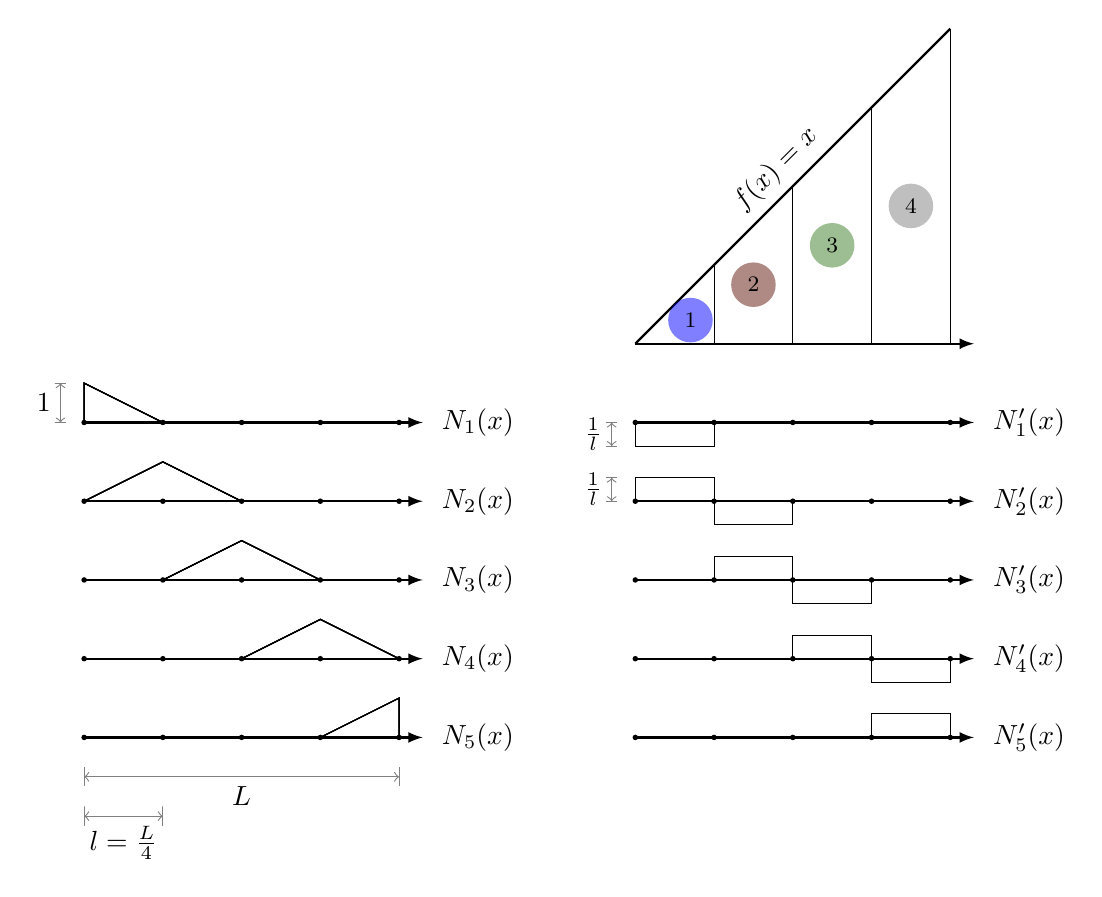
\begin{tikzpicture}[x=1cm,y=1cm]
  \begin{scope}
    % \draw[style=help lines,step=1cm] (0,-1) grid (11,5);

    \foreach \y in {0,1,2,3,4}{%
      \foreach \x in {0,7}{%
        \draw[-latex,thick] (\x,\y) -- +(4.3,0);
        \foreach \z in {0,1,2,3,4}{
          \fill[black] (\x + \z, \y) circle (1pt);
        }
      }



      \newcommand{\myh}{0.5}
      \draw (0,4) -- ++(0,\myh) -- ++(1,-\myh);
      \draw (3,0) -- ++(1,\myh) -- ++(0,-\myh);
      \foreach \i in {0,1,2}{
        \draw (\i, 3 - \i) -- ++(1,\myh) -- ++(1,-\myh);
      }
    }

    \foreach \i in {0,1,2,3}{
      \foreach \j in {0,0.7}{
        \draw (7 + \i, 3 - \i + \j) rectangle +(1,0.3);
      }
    }
    \foreach \y in {1,2,3,4,5}{
      % Label each diagram
      \node at (5, 5 - \y) {$N_{\y}(x)$};
      \node at (5 + 7, 5 - \y) {$N_{\y}'(x)$};
    }

  \end{scope}

  \newdimen\h
  \h=3.5pt

  % Draw the two dimensions
  \begin{scope}[draw=black!50]
    \foreach \i / \j / \l in {0.5 / 4 / L, 1 / 1 / l=\frac{L}{4}}{
      \draw[thin,<->] (0,-\i) to node[anchor=north] {$\l$} +(\j,0);
      \draw (0,-\i) -- +(0,\h) -- +(0, -\h)
      (\j,-\i) -- +(0,\h) -- +(0, -\h);
    }

    \h=2pt
    \newcommand{\mydimy}[4]{%
      \draw[thin,<->] (#1,#2) to node[left] {#4} +(0,#3);
      \draw (#1,#2) -- +(-\h,0) -- +(\h,0)
      (#1,#2 + #3) --  +(-\h,0) -- +(\h,0);
    }
    % \draw[thin,<->] (-0.3,4) to node[left] {1} +(0,0.5);
    % \draw (-0.3,4) -- +(-\h,0) -- +(\h,0)
    % (-0.3,4 + 0.5) --  +(-\h,0) -- +(\h,0);
    \mydimy{-0.3}{4}{0.5}{1}
    \mydimy{7-0.3}{3}{0.3}{$\frac{1}{l}$}
    \mydimy{7-0.3}{3.7}{0.3}{$\frac{1}{l}$}
  \end{scope}

  \begin{scope}[xshift=7cm,yshift=5cm]
    \draw[-latex,thick] (0,0) -- +(4.3,0);
    \draw[thick] (0,0) to node[sloped,above]{$f(x)=x$} (4,4);
    \foreach \x in {1,2,3,4}{
      \draw (\x,0) -- (\x,\x);
    }

    \newcommand{\mynode}[3][(0,0)]{
      \node[shape=circle, fill=#3,
      fill opacity=0.5,text opacity=1,font=\footnotesize, shift={#1}] {#2};
      % \node[shape=circle, fill=gray,
      % fill opacity=0.5,text opacity=1,font=\footnotesize, shift={(1cm,1cm)}] {2};
    }
    % \foreach \i/\j/\c in {0.5/1/\mycola,1.3/2/\mycolb,2.3/3/\mycolc,3.3/4/gray}{
    %   \mynode[(\i + 0.2, \i -0.2)]{\j}{\c}
    % }
    \mynode[(0.7, 0.3)]{1}{\mycola}
    \mynode[(1.5,0.75)]{2}{\mycolb}
    \mynode[(2.5,1.25)]{3}{\mycolc}
    \mynode[(3.5,1.75)]{4}{gray}
    % \mynode[(0.5 + 0.2, 0.5 -0.2)]{2}{\mycolb}
    % \mynode[(0.5 + 0.2, 0.5 -0.2)]{3}{\mycolc}
  \end{scope}

\end{tikzpicture}
  \caption{Shape functions and their derivative}\label{fig:shpfuncs}
\end{figure}
\subsubsection*{Calculate $K_{ij}$}
The shape functions and their derivatives are presented on \cref{fig:shpfuncs}.
We first calculate the diagonal entries:


\newcommand{\mynode}[3][]{
  \begin{tikzpicture}
    \def\h{17pt}
    \useasboundingbox (0,0) rectangle (\h,\h);
    \node[shape=circle, fill=#3,
    fill opacity=0.5,text opacity=1,font=\footnotesize, shift={(8.5pt,3pt)}] {#2};
  \end{tikzpicture}
}

\newcommand{\na}{\mynode{1}{\mycola}}
\newcommand{\nb}{\mynode{2}{\mycolb}}
\newcommand{\nc}{\mynode{3}{\mycolc}}
\newcommand{\nd}{\mynode{4}{gray}}

\begin{align}
  K_{11} &= \i{x N_0' N_0'}
           = [\text{area of \na on \cref{fig:shpfuncs}}]
           \times {[\text{the slope of shape function}]}^2
           :=  \na \times s \label{eq:k11}\\
  K_{22} &= \i{xN_1' N_1'} = [\text{area of \na{} $+$ \nb{}}]
           \times {[\text{the slope of shape function}]}^2
           := (\na{} + \nb{}) \times s \label{eq:k22}\\
  \intertext{Similarly}
  K_{33} & = (\nb{} + \nc{}) \times s \label{eq:k33}\\
  K_{44} & = (\nc{} + \nd{}) \times s \label{eq:k44}\\
  K_{55} &= (\nd{}) \times s \label{eq:k55}
\end{align}
Note that in \cref{eq:k11,eq:k22,eq:k33,eq:k44,eq:k55}, they are all multiplied by the same value $s = \frac{1}{l^2}$, even if
the slope is sometimes positive and sometimes negative. This is because, when
they are squared, they are always positive.

Now the areas can be calculated as follows:
\begin{align}
  \na &= \frac{l^2}{2} \label{eq:na}\\
  \nb &= l^2 + \na = \frac{3}{2}l^2 \label{eq:nb}\\
  \nc &= l^2 + \nb = \frac{5}{2}l^2 \label{eq:nc}\\
  \nd &= l^2 + \nc = \frac{7}{2}l^2 \label{eq:nd}
\end{align}
Substituting \cref{eq:na,eq:nb,eq:nc,eq:nd} back into
\cref{eq:k11,eq:k22,eq:k33,eq:k44,eq:k55} gives
\begin{align}
  K_{11} &=  \na \times s =
           \frac{l^2}{2} \times \frac{1}{l^2}
           = \frac{1}{2}\label{eq:nk11}\\
  K_{22} &= (\na{} + \nb{}) \times s =
           (\frac{l^2}{2} + \frac{3}{2}l^2) \frac{1}{l^2} =
           \frac{1}{2} + \frac{3}{2} = \frac{4}{2}
           \label{eq:nk22}\\
  K_{33} & = (\nb{} + \nc{}) \times s
           (\frac{3}{2}l^2 + \frac{5}{2}l^2) \frac{1}{l^2} =
           \frac{3}{2} + \frac{5}{2} = \frac{8}{2}
           \label{eq:nk33}\\
  K_{44} & = (\nc{} + \nd{}) \times s =
           \frac{5}{2} + \frac{7}{2} = \frac{23}{2}
           \label{eq:nk44}\\
  K_{55} &= \nd{} \times s = \frac{7}{2}
           \label{eq:nk55}
\end{align}

Now for the off-diagonal entries, because
\def\K{\ensuremath{\mathbf{K}}}
\begin{enumerate}
\item $\K$ is symmetrical ($K_{ij} = K_{ji}$)
\item the product of two node's shape functions is zero if the nodes are not
  next to each other
\end{enumerate}
the only entries that we need to calculate are the following
\begin{align}
  K_{12} &
           = [\text{area of \na{} on \cref{fig:shpfuncs}}]
           \times - {[\text{the slope of shape function}]}^2
           = \na{} \times (-s)  = -\frac{1}{2}\label{eq:nk12}\\
  K_{23} &= \nb{} \times (-s) = -\frac{3}{2}\label{eq:nk23}\\
  K_{34} &= \nc{} \times (-s) = -\frac{5}{2}\label{eq:nk34}\\
  K_{45} &= \nd{} \times (-s) = -\frac{7}{2}\label{eq:nk45}
\end{align}

Combining
\cref{eq:nk12,eq:nk23,eq:nk34,eq:nk45,eq:nk11,eq:nk22,eq:nk33,eq:nk44,eq:nk55}
gives the matrix $\K$
\def\matK{\ensuremath{\frac{1}{2}
    \begin{bmatrix}
      1 & -1 &&&\\
      -1 &4&-3&&\\
      & -3 &8&-5&\\
      &&-5&12&-7\\
      &&&-7&7
    \end{bmatrix}
  }}
\begin{align}
  \K &=
               \begin{bmatrix}
                 K_{11} & K_{12} &&&\\
                 K_{12} & K_{22} &K_{23}&&\\
                 & K_{23} &K_{33}&K_{34}&\\
                 &&K_{34}&K_{44}&K_{45}\\
                 &&&K_{45}&K_{55}
               \end{bmatrix} = \matK{} \label{eq:bigK}
\end{align}
In \cref{eq:bigK}, empty entry implies zero.

\subsubsection*{Calculate $L_{ij}$}
\def\L{\ensuremath{\mathbf{L}}}
Before we calculate \L, we calculate two \emph{convolution integrals}
% Triangle A
\newcommand{\Ta}{
  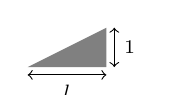
\begin{tikzpicture}
    \tikzstyle{every node}=[font=\scriptsize]
    \def\w{1cm}
    \def\h{0.5cm}
    \useasboundingbox (0,0) rectangle (\w + 15pt, \h);
    \fill[gray] (0,0) -- (\w,\h) -- (\w,0) -- cycle;
    % Draw the two dimensions
    % \def\h{3.5pt}
    \def\i{0.1cm}
    \draw[thin,<->] (0,-\i) to node[below] {$l$} +(\w,0);
    \draw[thin,<->] (\w + \i,0) to node[right] {1} +(0,\h);
  \end{tikzpicture}
}
% Triangle B
\newcommand{\Tb}{
  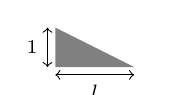
\begin{tikzpicture}
    \tikzstyle{every node}=[font=\scriptsize]
    \def\w{1cm}
    \def\h{0.5cm}
    \useasboundingbox (-10pt,0) rectangle (\w + 5pt, \h);
    \fill[gray] (0,0) -- (0,\h) -- (\w,0) -- cycle;
    \def\i{0.1cm}
    \draw[thin,<->] (0,-\i) to node[below] {$l$} +(\w,0);
    \draw[thin,<->] (-\i,0) to node[left] {1} +(0,\h);
  \end{tikzpicture}
}

\newcommand{\il}[1]{\ensuremath{\int_0^l #1 dx}}
\newcommand{\brkIt}[1]{\ensuremath{\left[#1\right]}}
\newcommand{\brkItl}[1]{\ensuremath{{\brkIt{#1}}_0^l}}
\newcommand{\prnIt}[1]{\ensuremath{\left( #1 \right)}}
\def\xl{\ensuremath{{\left( \frac{x}{l} \right)}^2}}
% \def\a{\cla{a}}
% \def\b{\clb{b}}
\def\a{\tcbox[on line,size=small,colback=\mycola!20,colframe=\mycola]{a}}
\def\b{\tcbox[on line,size=small,colback=\mycolb!20,colframe=\mycolb]{b}}
\def\anum{\ensuremath{\alpha\frac{l}{3}}}
\def\bnum{\ensuremath{\alpha\frac{l^2}{2} - \anum }}
\def\bnumb{\ensuremath{\alpha\frac{l}{6}(3l-2)}}
\begin{align}
  \a &:= \alpha \il{\Ta \Ta} = \alpha  \il{\xl{}} \notag\\
  &= \alpha \frac{1}{l^2} \brkItl{\frac{1}{3}x^3}
  = \frac{l^3}{3l^2} = \anum \\[\baselineskip]
  \b &:= \alpha \il{\Ta \Tb } = \alpha  \il{\frac{x}{l} (l - \frac{x}{l})} \notag\\
    &= \alpha\il{x} - \alpha \il{\xl{}}
      = \alpha\brkItl{\frac{x^2}{2}} - \a \notag\\
  &= \bnum =  \bnumb
\end{align}
Now, because $L_{ij} := \alpha \i{N_i N_j}$, from \cref{fig:shpfuncs} we see
that
\begin{align}
  L_{11} &= L_{55} = \a  = \anum \label{eq:l1}\\
  L_{22} &= L_{33} = L_{44} = 2 \times \a = \alpha\frac{2l}{3} \label{eq:l2}\\
  L_{12} &= L_{23} = L_{34} = L_{45} = \b = \bnumb \label{eq:l3}
\end{align}
\def\L{\ensuremath{\mathbf{L}}}
Since \L \ has the same properties as \K \
(i.e.,being symmetrical, non-neibour entries have value of 0).
Combining \cref{eq:l1,eq:l2,eq:l3} gives the matrix \L
\def\x{3l-2}
\begin{align}
  \mathbf{L} &=
               \begin{bmatrix}
                 L_{11} & L_{12} &&&\\
                 L_{12} & L_{22} &L_{23}&&\\
                 & L_{23} &L_{33}&L_{34}&\\
                 &&L_{34}&L_{44}&L_{45}\\
                 &&&L_{45}&L_{55}
               \end{bmatrix}
                            =
                            \frac{\alpha l}{6}
                            \begin{bmatrix}
                              2& c &&&\\
                              c &4&c&&\\
                              & c &4&c&\\
                              &&c&4&c\\
                              &&&c&2
                            \end{bmatrix} \label{eq:bigL}\\
  c &:= \x \notag
\end{align}
In \cref{eq:bigL}, empty entry implies zero.

\subsubsection*{Calculate $b_i$}
\def\b{\ensuremath{\mathbf{b}}}
\def\matb{\ensuremath{
    \begin{bmatrix}
      1 \\ 2  \\ 2 \\ 2 \\ 1
    \end{bmatrix}
  }}
The last array needed for \cref{eq:mtb} is \b \ where
\def\aTi{\ensuremath{\alpha T_{\infty}}}
\def\A{\tcbox[on line,size=small,colback=\mycolc!20,colframe=\mycolc]{A}}
\def\alT{\ensuremath{\alpha T_{\infty}}}
\begin{align}
  \clc{b_i} :&= \clc{\aTi \i{N_i}} \notag\\
             &= \aTi  \times [\text{The area under shape function \ } N_i(x)] \notag\\
  \intertext{Therefore}
  \b &= \A \matb
       \quad \text{where \ } \A = \alT \times \left[
       \text{area of \Ta}  = \frac{l}{2} \right] \label{eq:bigb}
\end{align}

\subsubsection*{Back to the system}
Now, substituting \cref{eq:bigc,eq:bigK,eq:bigL,eq:bigb} back into \cref{eq:mtb} gives
the system
\def\M{\ensuremath{\mathbf{M}}}
\def\matM{\ensuremath{
    \begin{bmatrix}
      \frac{\alpha}{3} + \frac{1}{2} & \frac{\alpha}{6} - \frac{1}{2} &&&\\
      \frac{\alpha}{6} - \frac{1}{2} & \frac{2 \alpha}{3} + 2& \frac{\alpha}{6} - \frac{3}{2} &&\\
       &\frac{\alpha}{6} - \frac{3}{2}&\frac{2 \alpha}{3} + 4& \frac{\alpha}{6} - \frac{5}{2} &\\
       && \frac{\alpha}{6} - \frac{5}{2}&\frac{2 \alpha}{3} + 6& \frac{\alpha}{6} - \frac{7}{2}\\
       &&& \frac{\alpha}{6} - \frac{7}{2}&\frac{\alpha}{3} + \frac{7}{2}
      \end{bmatrix}
  }}
\def\matMmoved{\ensuremath{
    \begin{bmatrix}
      \frac{\alpha}{3} + \frac{1}{2} & \frac{\alpha}{6} - \frac{1}{2} &&\\
      \frac{\alpha}{6} - \frac{1}{2} & \frac{2 \alpha}{3} + 2& \frac{\alpha}{6} - \frac{3}{2} &\\
      &\frac{\alpha}{6} - \frac{3}{2}&\frac{2 \alpha}{3} + 4& \frac{\alpha}{6} - \frac{5}{2} \\
      && \frac{\alpha}{6} - \frac{5}{2}&\frac{2 \alpha}{3} + 6\\
      &&& \frac{\alpha}{6} - \frac{7}{2}
    \end{bmatrix}
  }
}

\begin{align}
  \M &= \L + \K =
  \frac{\alpha l}{6}
  \begin{bmatrix}
    2& c &&&\\
    c &4&c&&\\
    & c &4&c&\\
    &&c&4&c\\
    &&&c&2
  \end{bmatrix} + \matK \notag\\
  c &= \x \notag\\
  \b &=\alT \frac{l}{2}\begin{bmatrix}1&2&2&2&1\end{bmatrix}^{\text{T}} \notag\\
  \intertext{Substituting $l = \frac{4}{4} = 1$
  gives}
  c &= 1 \notag\\
  \M &=
       \frac{\alpha}{6}
       \begin{bmatrix}
         2& 1 &&&\\
         1 &4&1&&\\
         & 1 &4&1&\\
         &&1&4&1\\
         &&&1&2
       \end{bmatrix} + \matK \notag\\
     &=\MyGet{M} \label{eq:bigM}\\
  \b &=\alT \frac{1}{2}\begin{bmatrix}1&2&2&2&1\end{bmatrix}^{\text{T}} \notag \\
\end{align}
Therefore the system in \cref{eq:mtb} becomes
\begin{align}
  \MyGet{M}
  \begin{bmatrix} T_1 \\ T_2 \\ T_3 \\ T_4 \\ T_5 \end{bmatrix}
  &= \alT \frac{1}{2} \matb +
    \begin{bmatrix}
      0\\0\\0\\0\\ s
    \end{bmatrix} \label{eq:readyToSplit}\\
  s&= \eBdri{L} \notag
\end{align}
Because of boundary condition \cref{eq:bc2}, $T_5=T_0$ is known, therefore the
unknowns are:
\begin{itemize}
\item the node temperatures $T_1$ to $T_4$. [4 unknowns]
\item $s$,the heat flow per unit time at $x=L$ [1 unknown]
\end{itemize}
Therefore there are 5 equations and 5 unknowns.
We follow the following steps:
\begin{enumerate}
\item Solve for $T_1$ to $T_4$
\item Find $s$, 
\end{enumerate}
\subsubsection*{Solve for $T_1$ to $T_4$}
Moving $T_5$ to the RHS of \cref{eq:readyToSplit} gives
\def\Tn{\ensuremath{\begin{bmatrix} T_1 \\ T_2 \\ T_3 \\ T_4 \end{bmatrix}}}
\def\alTt{\ensuremath{\alT \frac{1}{2}}}
\def\g#1{\MyGet{#1}}
\begin{align}
  \g{M2} \Tn
    &= \alTt \matb +
    \begin{bmatrix}
      0\\0\\0\\0\\ s
    \end{bmatrix} -
  T_5\g{Me} \label{eq:toDivide}\\
  s&= \eBdri{L} \notag
\end{align}
We divide \cref{eq:toDivide} into two pieces for our two steps:
\begin{align}
  \g{M.upper} \Tn &= \alTt \g{v.top} - T_5 \g{v2.top} \label{eq:mupper}\\
  \prnIt{\g{last.lhs}} T_4 &= \alTt + s  - T_5 \prnIt{\g{last.rhs}} \label{eq:mlower}
\end{align}
Substituting $\alpha = 0.4168, T_{\infty} = 75$ and $T_5 = T_0 = 250$ into
\cref{eq:mupper} gives
\begin{align}
  \g{M.upper.n} \Tn &= \g{rhs.upper} = \g{rhs.upper.n} \notag\\
  \intertext{Solving the system gives}
  \Tn &= \g{T1.T4} \label{eq:resultT}
\end{align}
Now substituting $T_4 = \g{T4.n}$ into \cref{eq:mlower} gives
\begin{align}
  s &= \eBdri{L} \notag\\
    &= \prnIt{\g{last.lhs}} \times T_4 + T_5 \prnIt{\g{last.rhs}} - \alTt \notag\\
    &= \prnIt{\g{last.lhs.n}} \times \g{T4.n} + 250 \times \g{last.rhs.n} - \g{alT2.n} \notag\\
  &= \g{s}
\end{align}
Which is the \emph{heat flow per unit time at $x=L$}
\subsubsection*{Remark}
As shown in \cref{eq:resultT}, the temperature $T$ gradually increases from $T_1 = \g{T1.n}$,
which is a bit higher than the ambient temperature $T_{\infty}$, to $T_4 =
\g{T4.n}$, which is a bit lower than the temperature, $T_5 = T_0 = 250$, at the
end $x=L$.

In order to be more accurate, finer mesh (i.e., more nodes) shall be used.

\section*{Question 2: fluid flow around a long cylinder}\label{sec:p2}

\MySet{A.a}{\left[\begin{matrix}1 &&\\1 & 5 &\\1 & 5 & 2\end{matrix}\right]}
\MySet{B.a}{\left[\begin{matrix}1 &&\\- \frac{1}{5} & \frac{1}{5} &\\& - \frac{1}{2} & \frac{1}{2}\end{matrix}\right]}
\MySet{B.r2.a}{\left[\begin{matrix}- \frac{1}{5} & \frac{1}{5} &\end{matrix}\right]}
\MySet{B.r2.t.a}{\left[\begin{matrix}- \frac{1}{5}\\\frac{1}{5}\\0\end{matrix}\right]}
\MySet{B.r3.a}{\left[\begin{matrix}& - \frac{1}{2} & \frac{1}{2}\end{matrix}\right]}
\MySet{B.r3.t.a}{\left[\begin{matrix}0\\- \frac{1}{2}\\\frac{1}{2}\end{matrix}\right]}
\MySet{Area.a}{5}
\MySet{K.a}{\left[\begin{matrix}\frac{1}{5} & - \frac{1}{5} &\\- \frac{1}{5} & \frac{29}{20} & - \frac{5}{4}\\& - \frac{5}{4} & \frac{5}{4}\end{matrix}\right]}
\MySet{K.g.a}{\left[\begin{matrix}\frac{1}{5} & - \frac{1}{5} &&&&&&&\\- \frac{1}{5} & \frac{29}{20} && - \frac{5}{4} &&&&&\\&&&&&&&&\\& - \frac{5}{4} && \frac{5}{4} &&&&&\\&&&&&&&&\\&&&&&&&&\\&&&&&&&&\\&&&&&&&&\\&&&&&&&&\end{matrix}\right]}
\MySet{poly.a}{\mathtt{\text{Path(array([[0.,.],
       [5.,.],
       [5., 2.],
       [0., 2.]]), None)}}}
\MySet{phis.a}{\left[, \ , \ .212121212121212, \ .212121212121212\right]}
\MySet{A.b}{\left[\begin{matrix}1 && 2\\1 & 5 & 2\\1 & 5 & 6\end{matrix}\right]}
\MySet{B.b}{\left[\begin{matrix}1 & \frac{1}{2} & - \frac{1}{2}\\- \frac{1}{5} & \frac{1}{5} &\\& - \frac{1}{4} & \frac{1}{4}\end{matrix}\right]}
\MySet{B.r2.b}{\left[\begin{matrix}- \frac{1}{5} & \frac{1}{5} &\end{matrix}\right]}
\MySet{B.r2.t.b}{\left[\begin{matrix}- \frac{1}{5}\\\frac{1}{5}\\0\end{matrix}\right]}
\MySet{B.r3.b}{\left[\begin{matrix}& - \frac{1}{4} & \frac{1}{4}\end{matrix}\right]}
\MySet{B.r3.t.b}{\left[\begin{matrix}0\\- \frac{1}{4}\\\frac{1}{4}\end{matrix}\right]}
\MySet{Area.b}{10}
\MySet{K.b}{\left[\begin{matrix}\frac{2}{5} & - \frac{2}{5} &\\- \frac{2}{5} & \frac{41}{40} & - \frac{5}{8}\\& - \frac{5}{8} & \frac{5}{8}\end{matrix}\right]}
\MySet{K.g.b}{\left[\begin{matrix}&&&&&&&&\\&&&&&&&&\\&& \frac{2}{5} & - \frac{2}{5} &&&&&\\&& - \frac{2}{5} & \frac{41}{40} &&&& - \frac{5}{8} &\\&&&&&&&&\\&&&&&&&&\\&&&&&&&&\\&&& - \frac{5}{8} &&&& \frac{5}{8} &\\&&&&&&&&\end{matrix}\right]}
\MySet{poly.b}{\mathtt{\text{Path(array([[0., 2.],
       [5., 2.],
       [5., 6.],
       [0., 6.]]), None)}}}
\MySet{phis.b}{\left[.212121212121212, \ .212121212121212, \  1, \  1\right]}
\MySet{A.c}{\left[\begin{matrix}1 & 5 &\\1 & 7 & 2\\1 & 5 & 2\end{matrix}\right]}
\MySet{B.c}{\left[\begin{matrix}1 & - \frac{5}{2} & \frac{5}{2}\\& \frac{1}{2} & - \frac{1}{2}\\- \frac{1}{2} && \frac{1}{2}\end{matrix}\right]}
\MySet{B.r2.c}{\left[\begin{matrix}& \frac{1}{2} & - \frac{1}{2}\end{matrix}\right]}
\MySet{B.r2.t.c}{\left[\begin{matrix}0\\\frac{1}{2}\\- \frac{1}{2}\end{matrix}\right]}
\MySet{B.r3.c}{\left[\begin{matrix}- \frac{1}{2} && \frac{1}{2}\end{matrix}\right]}
\MySet{B.r3.t.c}{\left[\begin{matrix}- \frac{1}{2}\\0\\\frac{1}{2}\end{matrix}\right]}
\MySet{Area.c}{2}
\MySet{K.c}{\left[\begin{matrix}\frac{1}{2} && - \frac{1}{2}\\& \frac{1}{2} & - \frac{1}{2}\\- \frac{1}{2} & - \frac{1}{2} & 1\end{matrix}\right]}
\MySet{K.g.c}{\left[\begin{matrix}&&&&&&&&\\& \frac{1}{2} && - \frac{1}{2} &&&&&\\&&&&&&&&\\& - \frac{1}{2} && 1 & - \frac{1}{2} &&&&\\&&& - \frac{1}{2} & \frac{1}{2} &&&&\\&&&&&&&&\\&&&&&&&&\\&&&&&&&&\\&&&&&&&&\end{matrix}\right]}
\MySet{poly.c}{\mathtt{\text{Path(array([[5.,.],
       [7., 2.],
       [5., 2.]]), None)}}}
\MySet{phis.c}{\left[, \ , \ .212121212121212\right]}
\MySet{A.d}{\left[\begin{matrix}1 & 5 & 2\\1 & 7 & 2\\1 & 5 & 6\end{matrix}\right]}
\MySet{B.d}{\left[\begin{matrix}4 & - \frac{5}{2} & - \frac{1}{2}\\- \frac{1}{2} & \frac{1}{2} &\\- \frac{1}{4} && \frac{1}{4}\end{matrix}\right]}
\MySet{B.r2.d}{\left[\begin{matrix}- \frac{1}{2} & \frac{1}{2} &\end{matrix}\right]}
\MySet{B.r2.t.d}{\left[\begin{matrix}- \frac{1}{2}\\\frac{1}{2}\\0\end{matrix}\right]}
\MySet{B.r3.d}{\left[\begin{matrix}- \frac{1}{4} && \frac{1}{4}\end{matrix}\right]}
\MySet{B.r3.t.d}{\left[\begin{matrix}- \frac{1}{4}\\0\\\frac{1}{4}\end{matrix}\right]}
\MySet{Area.d}{4}
\MySet{K.d}{\left[\begin{matrix}\frac{5}{4} & -1 & - \frac{1}{4}\\-1 & 1 &\\- \frac{1}{4} && \frac{1}{4}\end{matrix}\right]}
\MySet{K.g.d}{\left[\begin{matrix}&&&&&&&&\\&&&&&&&&\\&&&&&&&&\\&&& \frac{5}{4} & -1 &&& - \frac{1}{4} &\\&&& -1 & 1 &&&&\\&&&&&&&&\\&&&&&&&&\\&&& - \frac{1}{4} &&&& \frac{1}{4} &\\&&&&&&&&\end{matrix}\right]}
\MySet{poly.d}{\mathtt{\text{Path(array([[5., 2.],
       [7., 2.],
       [5., 6.]]), None)}}}
\MySet{phis.d}{\left[.212121212121212, \ , \  1\right]}
\MySet{A.e}{\left[\begin{matrix}1 & 7 & 2\\1 & 1& 4\\1 & 5 & 6\end{matrix}\right]}
\MySet{B.e}{\left[\begin{matrix}\frac{5}{2} & -2 & \frac{1}{2}\\- \frac{1}{8} & \frac{1}{4} & - \frac{1}{8}\\- \frac{5}{16} & \frac{1}{8} & \frac{3}{16}\end{matrix}\right]}
\MySet{B.r2.e}{\left[\begin{matrix}- \frac{1}{8} & \frac{1}{4} & - \frac{1}{8}\end{matrix}\right]}
\MySet{B.r2.t.e}{\left[\begin{matrix}- \frac{1}{8}\\\frac{1}{4}\\- \frac{1}{8}\end{matrix}\right]}
\MySet{B.r3.e}{\left[\begin{matrix}- \frac{5}{16} & \frac{1}{8} & \frac{3}{16}\end{matrix}\right]}
\MySet{B.r3.t.e}{\left[\begin{matrix}- \frac{5}{16}\\\frac{1}{8}\\\frac{3}{16}\end{matrix}\right]}
\MySet{Area.e}{8}
\MySet{K.e}{\left[\begin{matrix}\frac{29}{32} & - \frac{9}{16} & - \frac{11}{32}\\- \frac{9}{16} & \frac{5}{8} & - \frac{1}{16}\\- \frac{11}{32} & - \frac{1}{16} & \frac{13}{32}\end{matrix}\right]}
\MySet{K.g.e}{\left[\begin{matrix}&&&&&&&&\\&&&&&&&&\\&&&&&&&&\\&&&&&&&&\\&&&& \frac{29}{32} & - \frac{9}{16} && - \frac{11}{32} &\\&&&& - \frac{9}{16} & \frac{5}{8} && - \frac{1}{16} &\\&&&&&&&&\\&&&& - \frac{11}{32} & - \frac{1}{16} && \frac{13}{32} &\\&&&&&&&&\end{matrix}\right]}
\MySet{poly.e}{\mathtt{\text{Path(array([[ 7.,  2.],
       [10.,  4.],
       [ 5.,  6.]]), None)}}}
\MySet{phis.e}{\left[, \ , \  1\right]}
\MySet{A.f}{\left[\begin{matrix}1 & 1& 4\\1 & 1& 6\\1 & 5 & 6\end{matrix}\right]}
\MySet{B.f}{\left[\begin{matrix}3 & -4 & 2\\& \frac{1}{5} & - \frac{1}{5}\\- \frac{1}{2} & \frac{1}{2} &\end{matrix}\right]}
\MySet{B.r2.f}{\left[\begin{matrix}& \frac{1}{5} & - \frac{1}{5}\end{matrix}\right]}
\MySet{B.r2.t.f}{\left[\begin{matrix}0\\\frac{1}{5}\\- \frac{1}{5}\end{matrix}\right]}
\MySet{B.r3.f}{\left[\begin{matrix}- \frac{1}{2} & \frac{1}{2} &\end{matrix}\right]}
\MySet{B.r3.t.f}{\left[\begin{matrix}- \frac{1}{2}\\\frac{1}{2}\\0\end{matrix}\right]}
\MySet{Area.f}{5}
\MySet{K.f}{\left[\begin{matrix}\frac{5}{4} & - \frac{5}{4} &\\- \frac{5}{4} & \frac{29}{20} & - \frac{1}{5}\\& - \frac{1}{5} & \frac{1}{5}\end{matrix}\right]}
\MySet{K.g.f}{\left[\begin{matrix}&&&&&&&&\\&&&&&&&&\\&&&&&&&&\\&&&&&&&&\\&&&&&&&&\\&&&&& \frac{5}{4} &&& - \frac{5}{4}\\&&&&&&&&\\&&&&&&& \frac{1}{5} & - \frac{1}{5}\\&&&&& - \frac{5}{4} && - \frac{1}{5} & \frac{29}{20}\end{matrix}\right]}
\MySet{poly.f}{\mathtt{\text{Path(array([[10.,  4.],
       [10.,  6.],
       [ 5.,  6.]]), None)}}}
\MySet{phis.f}{\left[, \  1, \  1\right]}
\MySet{K.g.m1}{\left[\begin{matrix}\frac{2}{5} & - \frac{2}{5}\\- \frac{2}{5} & \frac{181}{40}\end{matrix}\right]}
\MySet{K.g.m2}{\left[\begin{matrix}&&\\& - \frac{7}{8} &\end{matrix}\right]}
\MySet{K.g.m1.inv}{\left[\begin{matrix}\frac{181}{66} & \frac{8}{33}\\\frac{8}{33} & \frac{8}{33}\end{matrix}\right]}
\MySet{K.g.m3}{\left[\begin{matrix}0\\\frac{7}{8}\end{matrix}\right]}
\MySet{K.g.sm}{\left[\begin{matrix}&& \frac{2}{5} & - \frac{2}{5} &&&&&\\& - \frac{7}{4} & - \frac{2}{5} & \frac{181}{40} & - \frac{3}{2} &&& - \frac{7}{8} &\end{matrix}\right]}
\MySet{K.g}{\left[\begin{matrix}\frac{1}{5} & - \frac{1}{5} &&&&&&&\\- \frac{1}{5} & \frac{39}{20} && - \frac{7}{4} &&&&&\\&& \frac{2}{5} & - \frac{2}{5} &&&&&\\& - \frac{7}{4} & - \frac{2}{5} & \frac{181}{40} & - \frac{3}{2} &&& - \frac{7}{8} &\\&&& - \frac{3}{2} & \frac{77}{32} & - \frac{9}{16} && - \frac{11}{32} &\\&&&& - \frac{9}{16} & \frac{15}{8} && - \frac{1}{16} & - \frac{5}{4}\\&&&&&&&&\\&&& - \frac{7}{8} & - \frac{11}{32} & - \frac{1}{16} && \frac{237}{160} & - \frac{1}{5}\\&&&&& - \frac{5}{4} && - \frac{1}{5} & \frac{29}{20}\end{matrix}\right]}
\MySet{phi3}{0.2121}
\MySet{phi4}{0.2121}
\MySet{b.n}{\left[\begin{matrix}0\\-0.3712\\0\\0\\-0.6619\\-1.313\\0\\1.096\\1.25\end{matrix}\right]}

\MySet{rec.Kx}{\left[\begin{matrix}2 & -2 & -1 & 1\\-2 & 2 & 1 & -1\\-1 & 1 & 2 & -2\\1 & -1 & -2 & 2\end{matrix}\right]}
\MySet{rec.Ky}{\left[\begin{matrix}2 & 1 & -1 & -2\\1 & 2 & -2 & -1\\-1 & -2 & 2 & 1\\-2 & -1 & 1 & 2\end{matrix}\right]}
\newcommand{\dXX}[2][x]{
  \ensuremath{\frac{\partial^2 #2}{\partial #1^2}}
}
\newcommand{\dX}[2][x]{
  \ensuremath{\frac{\partial #2}{\partial #1}}
}
\newcommand{\dxx}[1]{\dXX{#1}}
\newcommand{\dyy}[1]{\dXX[y]{#1}}
\newcommand{\dx}[1]{\dX{#1}}
\newcommand{\dy}[1]{\dX[y]{#1}}
\newcommand{\phin}{\ensuremath{
    \dX[\mathbf{n}]{\phi} 
  }}
\begin{questionbox}
  The function $\phi(x,y)$ is governed by
\begin{align}
\dxx{\phi} + \dyy{\phi} = 0 \label{eq:poi}
\end{align}
The mesh is shown in the following figure:

\newtcbox{bLabBox}[1][red]{
  on line,arc=0pt,colback=#1!10!white,
  colframe=#1!50!black,
  boxsep=0pt,left=1pt,right=1pt,top=2pt,
  bottom=2pt,boxrule=0pt,bottomrule=1pt,toprule=1pt
}
\newtcbox{nLabBox}[1][red]{
  on line,top=2pt,bottom=2pt,
  left=3pt,right=3pt,
  colframe=#1,
  colback=#1!10!white
}
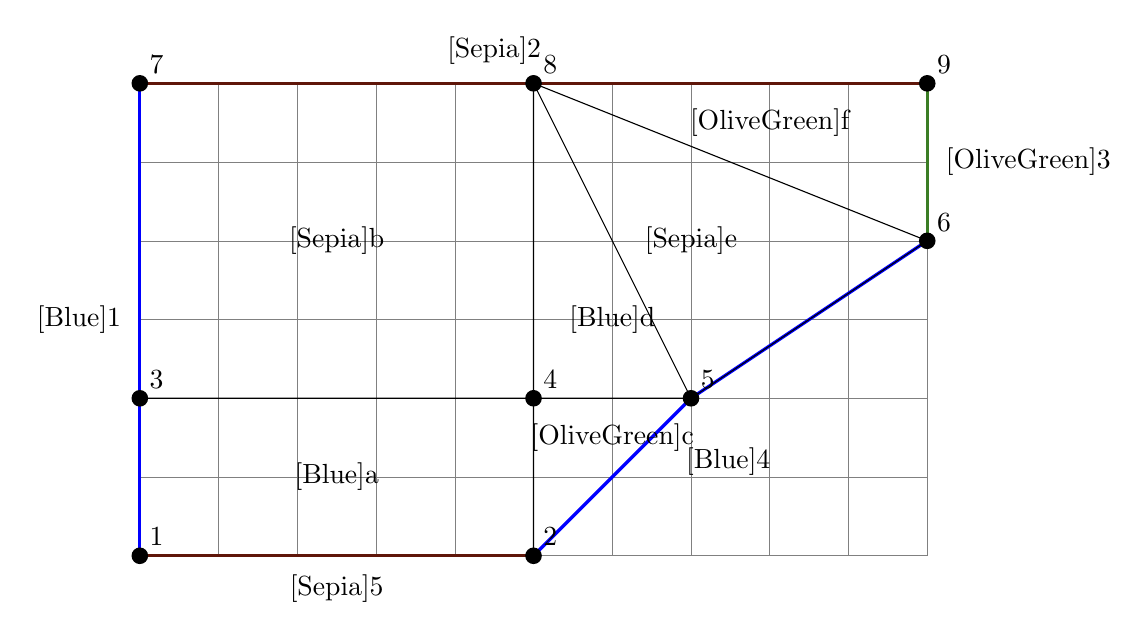
\begin{tikzpicture}[x=1cm,y=1cm]
  \newcommand{\bLab}[4][(0,0)]{
    % \node[fill=#2,text=white,#3] at #1 {#4};
    \node[#3] at #1 {
      \bLabBox[#2]{#4}
    };
  }

  \begin{scope}[very thick]
    \draw[style=help lines,step=1cm] (0,0) grid (10,6);
    % \tikzstyle{every node}=[draw,circle]

    \draw[draw=\mycola] (0,0) -- (0,6);
    \bLab[(0-0.1,3)]{\mycola}{left}{1}

    \draw[draw=\mycolb] (0,6) -- (10,6);
    \bLab[(4.5,6.1)]{\mycolb}{above}{2}

    \draw[draw=\mycolc] (10,6) -- (10,4);
    \bLab[(10.1,5)]{\mycolc}{right}{3}

    \draw[draw=\mycola] (10,4) -- (7,2) -- (5,0);
    \bLab[(7-0.2,1.2)]{\mycola}{right}{4}

    \draw[draw=\mycolb] (5,0) -- (0,0);
    \bLab[(2.5,-0.1)]{\mycolb}{below}{5}
  \end{scope}

  \begin{scope}
    % draw the mesh
    \draw (0,2) -- +(7,0)
    (5,0) -- ++(0,6)
     -- +(2,-4)
     -- +(5,-2)
     -- +(0,0);

     \foreach \x/\y/\l in {
       0/0/1,5/0/2,0/2/3,5/2/4,
       7/2/5,10/4/6,0/6/7,5/6/8,
       10/6/9}{
       \fill[black] (\x,\y) circle (3pt);
       \node[above right] at (\x,\y) {\l};
     }

     \newcommand{\nLab}[3][(0,0)]{
       % \node[fill=#2,text=white,rectangle] at #1 {#3};
       \node at #1 {\nLabBox[#2]{#3}};
     }

     \foreach \x/\y/\l/\c in {
       2.5/1/a/\mycola,2.5/4/b/\mycolb,
       6/1.5/c/\mycolc,6/3/d/\mycola,
       7/4/e/\mycolb,8/5.5/f/\mycolc
     }{\nLab[(\x,\y)]{\c}{\l}}
  \end{scope}
\end{tikzpicture}

\MySet{bd.col.1}{\mycola}
\MySet{bd.col.2}{\mycolb}
\MySet{bd.col.3}{\mycolc}
\MySet{bd.col.4}{\mycola}
\MySet{bd.col.5}{\mycolb}
\foreach \n/\i in {
  1/\mycola,
  2/\mycolb,
  3/\mycolc,
  4/\mycola,
  5/\mycolb}{
  \MySet{bd.col.\n}{\i}
}

\newcommand{\bd}[1]{\bLabBox[\MyGet{bd.col.#1}]{#1}}
\newcommand{\el}[1]{\nLabBox[\MyGet{el.col.#1}]{#1}}

% \foreach \n/\i in {
%   a/\mycola,
%   b/\mycolb,
%   c/\mycolc,
%   d/\mycola,
%   e/\mycolb,
%   f/\mycolc}{
%   \MySet{el.col.\n}{\i}
% }
% Don't know why it dosn't work   
\MySet{el.col.a}{\mycola}
\MySet{el.col.b}{\mycolb}
\MySet{el.col.c}{\mycolc}
\MySet{el.col.d}{\mycola}
\MySet{el.col.e}{\mycolb}
\MySet{el.col.f}{\mycolc}

Where \bd{1} to \bd{5} are boundaries,
and \el{a} to \el{f} are elements.

And the BCs are:
\def\f#1{\mbox{Along \bd{#1}: }}
\begin{align}
    \f{1} & \phin = 0 &  \f{2} & \phi = au_0 \notag\\
    \f{3} & \phin = 0 & \f{4} & \phi = 0 \notag\\ 
    \f{5} & \phi = 0 && \notag
\end{align}
\end{questionbox}

\subsection*{Answer}\label{sec:q2}
\subsubsection*{Weak formulation}
Let $v$ be an arbitrary test function, the weak formulation of \cref{eq:poi} is
then
\newcommand{\inta}[1]{
  \ensuremath{\int_{\text{Domain}} #1 \text{dA}}
}
\newcommand{\intb}[1]{
  \ensuremath{\int_{\text{Boundary}} #1 \text{ds}}
}

\def\x{
  \ensuremath{\inta{\nabla \phi \bullet \nabla v}}
}
\def\y{
  \ensuremath{\intb{\phin v}}
}


\begin{align}
  0 &= \inta{(\dxx{\phi} + \dyy{\phi}) v} \notag\\
  \intertext{By Gauss-Green}
    &= \inta{-\dx{\phi}\dx{v} - \dy{\phi}\dy{v}} +
      \intb{
      (\dx{\phi}\dx{n} + \dy{\phi}\dy{n})v
      } \notag\\
    &= -\x + \y \notag
\end{align}
Therefore,
\begin{align}
  \x &= \y \label{eq:tosub}
\end{align}
Now according to Galerkin's method, we take $v = \phi = N_j\phi_j$, which gives
\begin{align}
  \nabla v &= \nabla \phi = \nabla (N_i \phi_i) \notag\\
           &= \sum_i \phi_i \nabla N_i \notag\\
  &= \sum_i \phi_i
    \begin{bmatrix}
      \dx{N_i} \\ \dy{N_i}
    \end{bmatrix} \notag
\end{align}
Therefore, substituting the above into \cref{eq:tosub} gives
\def\x{\ensuremath{\inta{\nabla (N_i)\nabla (N_j)}}}
\def\bi{\ensuremath{\intb{\phin N_i}}}
\begin{align}
  \phi_i \inta{\nabla N_i \nabla N_j} \phi_j &= \intb{\phin N_j \phi_j} \notag\\
  \phi_i K_{ij} \phi_j &= b_i \phi_i \notag\\
  \intertext{Where}
  K_{ij} &= \x = \inta{\dx{N_i}\dx{N_j} + \dy{N_x}\dy{N_j}} \notag\\
  b_i &= \bi \notag
\end{align}
Taking derivatives with respect to $\mathbf{\phi} = [\phi_1, \dotsc, \phi_n]$,
and setting it to 0 gives the finite element equation
\def\tr#1{\ensuremath{{#1}^{\text{T}}}}
\def\p{\mathbf{\phi}}
\begin{align}
  \dX[\p]{\tr{\p} \mathbf{K} \p - \tr{\p}\mathbf{b}} &= 0 \quad \Rightarrow \quad
                                                       \mathbf{K}\p = \mathbf{b}
                                                       \label{eq:fe} \\
  \intertext{Where}
  \mathbf{K}_{ij} &= K_{ij} \quad \mathbf{b}_{i} &= b_i \notag
\end{align}
\def\K{\ensuremath{\mathbf{K}}}
We calculate \K element by element. But before we start, we derive the general
formulae that calculate the ``local stiffness matrix'' $K_{ij} = \x $ on a
rectangular element and a triangular element.

\subsubsection*{Local stiffness matrix for a rectangular element}
For a rectangular element as shown below

\begin{center}
  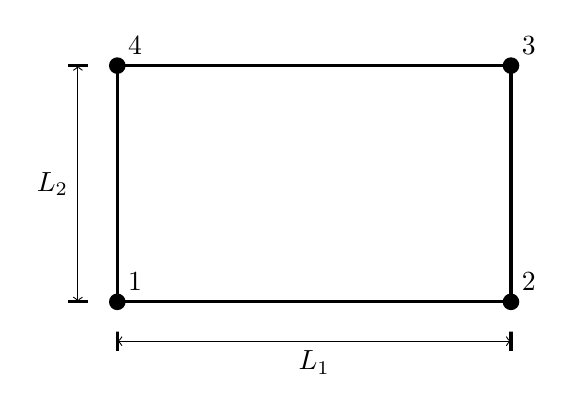
\begin{tikzpicture}[x=1cm,y=1cm]
  \begin{scope}[very thick]
    \draw (0,0) node[above right] (n1) {1}
    --  +(5,0) node[above right] (n2) {2}
    -- +(5,3) node[above right] (n3) {3}
    -- +(0,3) node[above right] (n4) {4}
    -- cycle;

    \foreach \i in {1,2,3,4}{
      % \node[fill=#2,]
      \fill[black] (n\i.south west) circle (3pt);
    }

    \newdimen\h
    \h=3.5pt
    % Draw the two dimensions
    \def\i{0.5cm}
    \def\j{5cm}

    \draw[thin,<->] (0,-\i) to node[anchor=north] {$L_1$} +(\j,0);
    \draw (0,-\i) -- +(0,\h) -- +(0, -\h)
    (\j,-\i) -- +(0,\h) -- +(0, -\h);

    % y dimensions
    \newcommand{\mydimy}[4]{%
      \draw[thin,<->] (#1,#2) to node[left] {#4} +(0,#3);
      \draw (#1,#2) -- +(-\h,0) -- +(\h,0)
      (#1,#2 + #3) --  +(-\h,0) -- +(\h,0);
    }
    \mydimy{-0.5cm}{0}{3}{$L_{2}$}
  \end{scope}
\end{tikzpicture}
\end{center}

\newcommand{\shpf}{shape functions}
The \shpf{} are
\newcommand{\Ni}[1]{\ensuremath{N_i(x,y)}}
\newcommand{\Nij}[2]{\dX[#2]{N_{#1}}}
\def\g#1{\ensuremath{g_{#1}(y)}}
\def\f#1{\ensuremath{f_{#1}(x)}}
\newcommand{\vg}{
  \begin{bmatrix}
    \g2 \\ \g1
  \end{bmatrix}
}

\begin{align}
  \begin{bmatrix}
    \Ni{4} & \Ni{3}\\
    \Ni{1} & \Ni{2}
  \end{bmatrix} &= \vg
             \begin{bmatrix}
               \f1 & \f2
             \end{bmatrix} \notag\\
  \intertext{Where}
  \begin{bmatrix}
    \f2\\ \f1
  \end{bmatrix}
           &=
             \begin{bmatrix}
               f_2\\f_1
             \end{bmatrix}
           =
                  \begin{bmatrix}
                    \frac{x}{L1} \\
                    1 - \f2
                  \end{bmatrix} \notag\\
  \vg &=
        \begin{bmatrix}
          g_2\\g_1
        \end{bmatrix}
           =
             \begin{bmatrix}
               \frac{y}{L2} \\
               1 - \g2
             \end{bmatrix} \notag
  \intertext{And their derivatives are}
  \begin{bmatrix}
    f_2' \\
    f_1'
  \end{bmatrix}
           &=
             \begin{bmatrix}
               \frac{1}{L1}\\
               - f_2'
             \end{bmatrix} \notag\\
  \begin{bmatrix}
    g_2' \\
    g_1'
  \end{bmatrix}
           &=
             \begin{bmatrix}
               \frac{1}{L2}\\
               - g_2'
             \end{bmatrix} \label{eq:fgvals}
\end{align}
Note that we have arranged the \shpf{} such that their position on the matrix above
are similar to their corresponding nodes on the figure above.

Now we calculate \Nij{i}{x} and \Nij{i}{y}
\newcommand{\Nx}{\ensuremath{\dx{\mathbf{N}}}}
\newcommand{\Ny}{\ensuremath{\dy{\mathbf{N}}}}

\def\mv#1#2{
  \ensuremath{\begin{bmatrix}#1 \\ #2\end{bmatrix}}
}
\def\mh#1#2{
  \ensuremath{\begin{bmatrix}#1 & #2\end{bmatrix}}
}
\def\x{\mv{g_2}{g_1}}
\def\y{
  % \ensuremath{\begin{bmatrix} f_1 & f_2 \end{bmatrix}}
  \ensuremath{\mh{f_1}{f_2}}
}
\begin{align}
  \Nx &=
        \begin{bmatrix}
          \Nij{4}{x} & \Nij{3}{x} \\
          \Nij{1}{x} & \Nij{2}{x} 
        \end{bmatrix}
                       = \x \mh{f_1'}{f_2'} = \x \mh{-f_2'}{f_2'}
                       = f_2' \x \mh{-1}{1}
                       \notag\\
  \Ny &=
        \begin{bmatrix}
          \Nij{4}{y} & \Nij{3}{y} \\
          \Nij{1}{y} & \Nij{2}{y} 
        \end{bmatrix}
                       = \mv{g_2'}{g_1'} \y = \mv{g_2'}{-g_2'} \y
                       = g_2'\mv{1}{-1} \y \notag
\end{align}
\def\Kx{\ensuremath{\mathbf{K_x}}}
\def\Ky{\ensuremath{\mathbf{K_y}}}
\newcommand{\Mij}[1]{
  \ensuremath{
    {\left[ #1 \right]}_{ij}
  }
}
Now er define two matrices \Kx and \Ky as follows:
\newcommand{\intc}[1]{
  \ensuremath{\int_0^{L2} \int_0^{L1} #1 \text{dxdy}}
}
\begin{align}
  \K &= \Kx + \Ky \notag\\
  \intertext{Where}
  \Mij{\Kx} &= \intc{\Nij{i}{x} \Nij{j}{x}} \notag\\
  \Mij{\Ky} &= \intc{\Nij{i}{y} \Nij{j}{y}} \notag
\end{align}
Next we flatten the (derivatives) \shpf{} matrices into column vectors by
defining:
\def\f#1{\ensuremath{N_{#1} &=
    \begin{bmatrix}
      \Nij{1}{#1} &
      \Nij{2}{#1} &
      \Nij{3}{#1} &
      \Nij{4}{#1} 
    \end{bmatrix}
  }
}
\begin{align}
  \f{x} \notag\\
  \f{y} \notag
\end{align}
So, $K_x$ and $K_y$ are
\begin{align}
  K_x &= \intc{\tr{N_x}N_x} \notag\\ 
  K_y &= \intc{\tr{N_y}N_y} \notag
\end{align}
Substituting the values in \cref{eq:fgvals} gives

\newcommand{\G}[1]{\MyGet{#1}}
\begin{align}
  K &= K_x + K_y \label{eq:recK} \\
  K_x &= \frac{1}{6} \frac{L_2}{L_1} \G{rec.Kx} \notag\\ 
  K_y &= \frac{1}{6} \frac{L_1}{L_2} \G{rec.Ky} \notag
\end{align}

\subsubsection*{Local stiffness matrix for a triangular element}
For a triangular element as shown below

\begin{center}
\begin{tikzpicture}[x=1cm,y=1cm]
  \begin{scope}
    \draw (0,0) coordinate (n1)
    --  +(4,-1) coordinate (n2) 
    -- +(3,2) coordinate (n3)
    -- cycle;

    \foreach \i/\p in {1/above left,2/below right,
      3/above left}{
      \node[\p] at (n\i) {$(x_{\i}, y_{\i})$};
      \fill[black] (n\i) circle (3pt);
    }
  \end{scope}
\end{tikzpicture}
\end{center}

The \shpf{} are
\def\N{\ensuremath{\mathbf{N}}}
\def\B{\ensuremath{\mathbf{B}}}
\def\A{\ensuremath{\mathbf{A}}}
\def\vxy{\ensuremath{\begin{bmatrix} 1&x&y \end{bmatrix}}}
\begin{align}
  \N &=
       \begin{bmatrix}
         \Ni{1} & \Ni{2} & \Ni{3} 
       \end{bmatrix} \notag\\
     &= \vxy \B = \vxy
       \begin{bmatrix} r_1 \\ r_2 \\ r_3 \end{bmatrix} \notag\\
  &= r_1 + xr_2 + yr_3
  \intertext{Where}
  r_i &= \text{The $i^{th}$ row of \B} \notag\\
  \B &= \A^{-1} \notag\\
  \A &=
       \begin{bmatrix}
         1 & x_1 & y_1 \\
         1 & x_2 & y_2 \\
         1 & x_3 & y_3 
       \end{bmatrix} \notag
\end{align}
Note that \shpf{} are linear, so their derivatives with respect to $x$ and $y$
are constant, which turns out to be entries in \B.
\def\f#1{
  \ensuremath{
    N_{#1} := \dX[#1]{\N} =
    \tr{
      \begin{bmatrix}
        \dX[#1]{N_1} &
        \dX[#1]{N_2} &
        \dX[#1]{N_3} 
      \end{bmatrix}
    }
      }
    }
\begin{align}
  \f{x} = r_2 \notag\\
  \f{y} = r_3 \notag
\end{align}
Similar to what we have done to for the rectanglar element, we define \Kx and
\Ky as follows:

\newcommand{\intd}[1]{
  \ensuremath{
    \int_{\text{A}}
    #1
    \text{dA}
  }
}
\def\f#1{
  \ensuremath{
    \Mij{K_{#1}} := \intd{\dX[#1]{N_i} \dX[#1]{N_j}}
  }
}
\def\dN#1{
  \ensuremath{\dX[#1]{\N}}
}
\def\dNdN#1{\tr{N_{x}}N_{x}}

\begin{align}
  \f{x} \notag\\
  \f{y}
  \notag
\end{align}
Where integrate over A means ``Integrate over the entire triangular element''.
However, since $N_x$ and $N_y$ are actually constant vector, therefore
\def\ar{ \text{area of triangular element}}
\begin{align}
  K_x  = \intd{\dNdN{x}} = r_2\tr{r_2} \intd{} = \ar \notag\\ 
  K_y = \intd{\dNdN{y}}  = r_2\tr{r_3} \intd{} = \ar \notag\\
  \intertext{So}
  \K = [r_2\tr{r_2} + r_3\tr{r_3}] \times \ar \label{eq:triK}
\end{align}

\subsubsection*{Calculate \K element by element}
\newcommand{\globalK}[1]{
  And its contribution to global stiffness matrix is
\begin{align}
  K_{#1,\text{global}} = \G{K.g.#1} \label{eq:K.g.#1}
\end{align}
}
\newcommand{\rec}[1]{%
  \paragraph{For element #1} applying \cref{eq:recK}
  with $L_1 =
  \G{l1.#1}, L_2 = \G{l2.#1}$ gives
\begin{align}
  K_{x,#1} &= \G{Kx.#1} \notag\\
  K_{y,#1} &= \G{Ky.#1} \notag\\
  K_{#1} &= \G{K.#1} \notag
\end{align}
\globalK{#1}
}
\newcommand{\tri}[1]{
  \paragraph{For element #1} applying \cref{eq:triK} with
  \begin{align*}
    \A = \begin{bmatrix}
      1 & x_1 & y_1 \\
      1 & x_2 & y_2 \\
      1 & x_3 & y_3 
    \end{bmatrix} = \G{A.#1}
  \end{align*} gives
  \begin{align}
    \B &= \A^{-1} = \G{B.#1} \notag\\
    \K &= \left[
         \G{B.r2.#1} \G{B.r2.t.#1}
         +
         \G{B.r3.#1} \G{B.r3.t.#1}
         \right]
         \G{Area.#1} \notag
\end{align}
\globalK{#1}
}
\rec{a}
\rec{b}
\tri{c}
\tri{d}
\tri{e}
\tri{f}
Now summing up \cref{eq:K.g.a,eq:K.g.b,eq:K.g.c,eq:K.g.d,eq:K.g.e,eq:K.g.f}
gives the global stiffness matrix \K
\begin{align}
  K_{\text{global}} &=
                      K_{a,\text{global}}
                      \foreach \i in {b,c,d,e,f}{
                      + 
                      K_{\i,\text{global}}
                      }\notag\\ 
  &= \G{K.g}
\end{align}

To finish \cref{eq:fe}, we apply the BCs, which can be more or less translated
into the following:
\def\DOF{degree of freedom}
\begin{quote}
  On all nodes except for node 3 and 4,
  the values of $\phi$ are known (so  \DOF{}$-7$). However, for each of these
  node (7 nodes), a nonzero value of $b_i = \bi$ is added for them.
\end{quote}
So
\def\au{\ensuremath{au_0}}
\begin{align}
  \mathbf{b} &=
               \tr{\begin{bmatrix}
                 b_1 & b_2 & 0&0&b_5&b_6&b_7&b_8&b_9
               \end{bmatrix}}
                                                  \notag\\
  \intertext{And}
  \mathbf{\phi}
             &=
                  \tr{\begin{bmatrix}
                      b_1 & b_2 & 0&0&b_5&b_6&b_7&b_8&b_9
                    \end{bmatrix}} \notag\\
             &=
               \tr{\begin{bmatrix}
                   \phi_1 , \dotsc \phi_9
                 \end{bmatrix}} \notag\\
             &=
               \tr{\begin{bmatrix}
                   0&0&\phi_3&\phi_4&0&0&\au&\au&\au
                 \end{bmatrix}}
\end{align}
So the system is therefore
\def\bn{\ensuremath{
    \begin{bmatrix}
      b_1 \\ b_2 \\ 0 \\ 0 \\ b_5 \\ b_6 \\ b_7 \\ b_8 \\ b_9 
    \end{bmatrix}}}
\def\phin{\ensuremath{
    \begin{bmatrix}
      0\\0\\\phi_3\\\phi_4\\0\\0\\ \au \\ \au \\ \au
    \end{bmatrix}}}
\begin{align*}
  \K \mathbf{\phi} = \mathbf{b} \notag\\
  \G{K.g} \phin = \bn \notag
\end{align*}
We first solve for $\phi_2$ and $\phi_3$
\def\one{\ensuremath{
    \begin{bmatrix} 1\\1\\1
    \end{bmatrix}}}
\def\pp{\ensuremath{
    \begin{bmatrix} \phi_3 \\ \phi_4
    \end{bmatrix}}}
\begin{align}
  \G{K.g.sm} \phin &= \bn \notag\\
  \G{K.g.m1} \pp &= - \G{K.g.m2} \one \au \notag\\
  \G{K.g.m1}^{-1} \pp &= \G{K.g.mi.inv} \notag\\
  -\au \G{K.g.m2} \one &= \au \G{K.g.m3} \notag\\
  \pp &= \au \begin{bmatrix} \G{phi3}\\\G{phi4} \end{bmatrix} \notag
\end{align}

And now $\mathbf{b}$ can be calculated as
\begin{align}
  \mathbf{b} = \au \G{K.g}
  \begin{bmatrix}
    0\\0\\\G{phi3}\\\G{phi4}\\0\\0\\ \au \\ \au \\ \au
  \end{bmatrix}
  = \au \G{b.n}
\end{align}

\subsubsection*{Remarks}
And the contour is shown below

% Created by tikzDevice version 0.12.3.1 on 2022-03-14 00:05:07
% !TEX encoding = UTF-8 Unicode
\begin{tikzpicture}[x=1pt,y=1pt]
\definecolor{fillColor}{RGB}{255,255,255}
\path[use as bounding box,fill=fillColor,fill opacity=0.00] (0,0) rectangle (433.62,216.81);
\begin{scope}
\path[clip] (  0.00,  0.00) rectangle (433.62,216.81);
\definecolor{drawColor}{RGB}{255,255,255}
\definecolor{fillColor}{RGB}{255,255,255}

\path[draw=drawColor,line width= 0.6pt,line join=round,line cap=round,fill=fillColor] (  0.00,  0.00) rectangle (433.62,216.81);
\end{scope}
\begin{scope}
\path[clip] ( 14.85, 18.22) rectangle (370.53,211.31);
\definecolor{fillColor}{gray}{0.92}

\path[fill=fillColor] ( 14.85, 18.22) rectangle (370.53,211.31);
\definecolor{drawColor}{RGB}{255,255,255}

\path[draw=drawColor,line width= 0.3pt,line join=round] ( 14.85, 53.73) --
	(370.53, 53.73);

\path[draw=drawColor,line width= 0.3pt,line join=round] ( 14.85,113.25) --
	(370.53,113.25);

\path[draw=drawColor,line width= 0.3pt,line join=round] ( 14.85,172.77) --
	(370.53,172.77);

\path[draw=drawColor,line width= 0.3pt,line join=round] ( 71.43, 18.22) --
	( 71.43,211.31);

\path[draw=drawColor,line width= 0.3pt,line join=round] (152.27, 18.22) --
	(152.27,211.31);

\path[draw=drawColor,line width= 0.3pt,line join=round] (233.10, 18.22) --
	(233.10,211.31);

\path[draw=drawColor,line width= 0.3pt,line join=round] (313.94, 18.22) --
	(313.94,211.31);

\path[draw=drawColor,line width= 0.6pt,line join=round] ( 14.85, 23.97) --
	(370.53, 23.97);

\path[draw=drawColor,line width= 0.6pt,line join=round] ( 14.85, 83.49) --
	(370.53, 83.49);

\path[draw=drawColor,line width= 0.6pt,line join=round] ( 14.85,143.01) --
	(370.53,143.01);

\path[draw=drawColor,line width= 0.6pt,line join=round] ( 14.85,202.53) --
	(370.53,202.53);

\path[draw=drawColor,line width= 0.6pt,line join=round] ( 31.02, 18.22) --
	( 31.02,211.31);

\path[draw=drawColor,line width= 0.6pt,line join=round] (111.85, 18.22) --
	(111.85,211.31);

\path[draw=drawColor,line width= 0.6pt,line join=round] (192.69, 18.22) --
	(192.69,211.31);

\path[draw=drawColor,line width= 0.6pt,line join=round] (273.52, 18.22) --
	(273.52,211.31);

\path[draw=drawColor,line width= 0.6pt,line join=round] (354.36, 18.22) --
	(354.36,211.31);
\definecolor{drawColor}{RGB}{20,45,69}
\definecolor{fillColor}{RGB}{20,45,69}

\path[draw=drawColor,line width= 0.4pt,line join=round,line cap=round,fill=fillColor] ( 31.02, 27.00) circle (  1.96);

\path[draw=drawColor,line width= 0.4pt,line join=round,line cap=round,fill=fillColor] ( 34.28, 27.00) circle (  1.96);

\path[draw=drawColor,line width= 0.4pt,line join=round,line cap=round,fill=fillColor] ( 37.55, 27.00) circle (  1.96);

\path[draw=drawColor,line width= 0.4pt,line join=round,line cap=round,fill=fillColor] ( 40.81, 27.00) circle (  1.96);

\path[draw=drawColor,line width= 0.4pt,line join=round,line cap=round,fill=fillColor] ( 44.08, 27.00) circle (  1.96);

\path[draw=drawColor,line width= 0.4pt,line join=round,line cap=round,fill=fillColor] ( 47.35, 27.00) circle (  1.96);

\path[draw=drawColor,line width= 0.4pt,line join=round,line cap=round,fill=fillColor] ( 50.61, 27.00) circle (  1.96);

\path[draw=drawColor,line width= 0.4pt,line join=round,line cap=round,fill=fillColor] ( 53.88, 27.00) circle (  1.96);
\definecolor{drawColor}{RGB}{20,44,69}
\definecolor{fillColor}{RGB}{20,44,69}

\path[draw=drawColor,line width= 0.4pt,line join=round,line cap=round,fill=fillColor] ( 57.14, 27.00) circle (  1.96);

\path[draw=drawColor,line width= 0.4pt,line join=round,line cap=round,fill=fillColor] ( 60.41, 27.00) circle (  1.96);

\path[draw=drawColor,line width= 0.4pt,line join=round,line cap=round,fill=fillColor] ( 63.68, 27.00) circle (  1.96);

\path[draw=drawColor,line width= 0.4pt,line join=round,line cap=round,fill=fillColor] ( 66.94, 27.00) circle (  1.96);

\path[draw=drawColor,line width= 0.4pt,line join=round,line cap=round,fill=fillColor] ( 70.21, 27.00) circle (  1.96);

\path[draw=drawColor,line width= 0.4pt,line join=round,line cap=round,fill=fillColor] ( 73.48, 27.00) circle (  1.96);

\path[draw=drawColor,line width= 0.4pt,line join=round,line cap=round,fill=fillColor] ( 76.74, 27.00) circle (  1.96);

\path[draw=drawColor,line width= 0.4pt,line join=round,line cap=round,fill=fillColor] ( 80.01, 27.00) circle (  1.96);

\path[draw=drawColor,line width= 0.4pt,line join=round,line cap=round,fill=fillColor] ( 83.27, 27.00) circle (  1.96);

\path[draw=drawColor,line width= 0.4pt,line join=round,line cap=round,fill=fillColor] ( 86.54, 27.00) circle (  1.96);

\path[draw=drawColor,line width= 0.4pt,line join=round,line cap=round,fill=fillColor] ( 89.81, 27.00) circle (  1.96);

\path[draw=drawColor,line width= 0.4pt,line join=round,line cap=round,fill=fillColor] ( 93.07, 27.00) circle (  1.96);

\path[draw=drawColor,line width= 0.4pt,line join=round,line cap=round,fill=fillColor] ( 96.34, 27.00) circle (  1.96);

\path[draw=drawColor,line width= 0.4pt,line join=round,line cap=round,fill=fillColor] ( 99.60, 27.00) circle (  1.96);

\path[draw=drawColor,line width= 0.4pt,line join=round,line cap=round,fill=fillColor] (102.87, 27.00) circle (  1.96);

\path[draw=drawColor,line width= 0.4pt,line join=round,line cap=round,fill=fillColor] (106.14, 27.00) circle (  1.96);

\path[draw=drawColor,line width= 0.4pt,line join=round,line cap=round,fill=fillColor] (109.40, 27.00) circle (  1.96);

\path[draw=drawColor,line width= 0.4pt,line join=round,line cap=round,fill=fillColor] (112.67, 27.00) circle (  1.96);

\path[draw=drawColor,line width= 0.4pt,line join=round,line cap=round,fill=fillColor] (115.93, 27.00) circle (  1.96);

\path[draw=drawColor,line width= 0.4pt,line join=round,line cap=round,fill=fillColor] (119.20, 27.00) circle (  1.96);

\path[draw=drawColor,line width= 0.4pt,line join=round,line cap=round,fill=fillColor] (122.47, 27.00) circle (  1.96);

\path[draw=drawColor,line width= 0.4pt,line join=round,line cap=round,fill=fillColor] (125.73, 27.00) circle (  1.96);
\definecolor{drawColor}{RGB}{20,44,68}
\definecolor{fillColor}{RGB}{20,44,68}

\path[draw=drawColor,line width= 0.4pt,line join=round,line cap=round,fill=fillColor] (129.00, 27.00) circle (  1.96);

\path[draw=drawColor,line width= 0.4pt,line join=round,line cap=round,fill=fillColor] (132.26, 27.00) circle (  1.96);

\path[draw=drawColor,line width= 0.4pt,line join=round,line cap=round,fill=fillColor] (135.53, 27.00) circle (  1.96);

\path[draw=drawColor,line width= 0.4pt,line join=round,line cap=round,fill=fillColor] (138.80, 27.00) circle (  1.96);

\path[draw=drawColor,line width= 0.4pt,line join=round,line cap=round,fill=fillColor] (142.06, 27.00) circle (  1.96);

\path[draw=drawColor,line width= 0.4pt,line join=round,line cap=round,fill=fillColor] (145.33, 27.00) circle (  1.96);

\path[draw=drawColor,line width= 0.4pt,line join=round,line cap=round,fill=fillColor] (148.60, 27.00) circle (  1.96);
\definecolor{drawColor}{RGB}{19,44,68}
\definecolor{fillColor}{RGB}{19,44,68}

\path[draw=drawColor,line width= 0.4pt,line join=round,line cap=round,fill=fillColor] (151.86, 27.00) circle (  1.96);

\path[draw=drawColor,line width= 0.4pt,line join=round,line cap=round,fill=fillColor] (155.13, 27.00) circle (  1.96);

\path[draw=drawColor,line width= 0.4pt,line join=round,line cap=round,fill=fillColor] (158.39, 27.00) circle (  1.96);

\path[draw=drawColor,line width= 0.4pt,line join=round,line cap=round,fill=fillColor] (161.66, 27.00) circle (  1.96);

\path[draw=drawColor,line width= 0.4pt,line join=round,line cap=round,fill=fillColor] (164.93, 27.00) circle (  1.96);

\path[draw=drawColor,line width= 0.4pt,line join=round,line cap=round,fill=fillColor] (168.19, 27.00) circle (  1.96);

\path[draw=drawColor,line width= 0.4pt,line join=round,line cap=round,fill=fillColor] (171.46, 27.00) circle (  1.96);

\path[draw=drawColor,line width= 0.4pt,line join=round,line cap=round,fill=fillColor] (174.72, 27.00) circle (  1.96);

\path[draw=drawColor,line width= 0.4pt,line join=round,line cap=round,fill=fillColor] (177.99, 27.00) circle (  1.96);

\path[draw=drawColor,line width= 0.4pt,line join=round,line cap=round,fill=fillColor] (181.26, 27.00) circle (  1.96);

\path[draw=drawColor,line width= 0.4pt,line join=round,line cap=round,fill=fillColor] (184.52, 27.00) circle (  1.96);

\path[draw=drawColor,line width= 0.4pt,line join=round,line cap=round,fill=fillColor] (187.79, 27.00) circle (  1.96);

\path[draw=drawColor,line width= 0.4pt,line join=round,line cap=round,fill=fillColor] (191.05, 27.00) circle (  1.96);
\definecolor{drawColor}{RGB}{19,43,67}
\definecolor{fillColor}{RGB}{19,43,67}

\path[draw=drawColor,line width= 0.4pt,line join=round,line cap=round,fill=fillColor] (194.32, 27.00) circle (  1.96);
\definecolor{drawColor}{RGB}{21,47,72}
\definecolor{fillColor}{RGB}{21,47,72}

\path[draw=drawColor,line width= 0.4pt,line join=round,line cap=round,fill=fillColor] ( 31.02, 30.02) circle (  1.96);

\path[draw=drawColor,line width= 0.4pt,line join=round,line cap=round,fill=fillColor] ( 34.28, 30.02) circle (  1.96);

\path[draw=drawColor,line width= 0.4pt,line join=round,line cap=round,fill=fillColor] ( 37.55, 30.02) circle (  1.96);

\path[draw=drawColor,line width= 0.4pt,line join=round,line cap=round,fill=fillColor] ( 40.81, 30.02) circle (  1.96);

\path[draw=drawColor,line width= 0.4pt,line join=round,line cap=round,fill=fillColor] ( 44.08, 30.02) circle (  1.96);

\path[draw=drawColor,line width= 0.4pt,line join=round,line cap=round,fill=fillColor] ( 47.35, 30.02) circle (  1.96);

\path[draw=drawColor,line width= 0.4pt,line join=round,line cap=round,fill=fillColor] ( 50.61, 30.02) circle (  1.96);
\definecolor{drawColor}{RGB}{21,46,72}
\definecolor{fillColor}{RGB}{21,46,72}

\path[draw=drawColor,line width= 0.4pt,line join=round,line cap=round,fill=fillColor] ( 53.88, 30.02) circle (  1.96);

\path[draw=drawColor,line width= 0.4pt,line join=round,line cap=round,fill=fillColor] ( 57.14, 30.02) circle (  1.96);

\path[draw=drawColor,line width= 0.4pt,line join=round,line cap=round,fill=fillColor] ( 60.41, 30.02) circle (  1.96);

\path[draw=drawColor,line width= 0.4pt,line join=round,line cap=round,fill=fillColor] ( 63.68, 30.02) circle (  1.96);

\path[draw=drawColor,line width= 0.4pt,line join=round,line cap=round,fill=fillColor] ( 66.94, 30.02) circle (  1.96);
\definecolor{drawColor}{RGB}{21,46,71}
\definecolor{fillColor}{RGB}{21,46,71}

\path[draw=drawColor,line width= 0.4pt,line join=round,line cap=round,fill=fillColor] ( 70.21, 30.02) circle (  1.96);

\path[draw=drawColor,line width= 0.4pt,line join=round,line cap=round,fill=fillColor] ( 73.48, 30.02) circle (  1.96);

\path[draw=drawColor,line width= 0.4pt,line join=round,line cap=round,fill=fillColor] ( 76.74, 30.02) circle (  1.96);

\path[draw=drawColor,line width= 0.4pt,line join=round,line cap=round,fill=fillColor] ( 80.01, 30.02) circle (  1.96);

\path[draw=drawColor,line width= 0.4pt,line join=round,line cap=round,fill=fillColor] ( 83.27, 30.02) circle (  1.96);

\path[draw=drawColor,line width= 0.4pt,line join=round,line cap=round,fill=fillColor] ( 86.54, 30.02) circle (  1.96);

\path[draw=drawColor,line width= 0.4pt,line join=round,line cap=round,fill=fillColor] ( 89.81, 30.02) circle (  1.96);

\path[draw=drawColor,line width= 0.4pt,line join=round,line cap=round,fill=fillColor] ( 93.07, 30.02) circle (  1.96);

\path[draw=drawColor,line width= 0.4pt,line join=round,line cap=round,fill=fillColor] ( 96.34, 30.02) circle (  1.96);

\path[draw=drawColor,line width= 0.4pt,line join=round,line cap=round,fill=fillColor] ( 99.60, 30.02) circle (  1.96);

\path[draw=drawColor,line width= 0.4pt,line join=round,line cap=round,fill=fillColor] (102.87, 30.02) circle (  1.96);
\definecolor{drawColor}{RGB}{20,46,71}
\definecolor{fillColor}{RGB}{20,46,71}

\path[draw=drawColor,line width= 0.4pt,line join=round,line cap=round,fill=fillColor] (106.14, 30.02) circle (  1.96);

\path[draw=drawColor,line width= 0.4pt,line join=round,line cap=round,fill=fillColor] (109.40, 30.02) circle (  1.96);

\path[draw=drawColor,line width= 0.4pt,line join=round,line cap=round,fill=fillColor] (112.67, 30.02) circle (  1.96);

\path[draw=drawColor,line width= 0.4pt,line join=round,line cap=round,fill=fillColor] (115.93, 30.02) circle (  1.96);

\path[draw=drawColor,line width= 0.4pt,line join=round,line cap=round,fill=fillColor] (119.20, 30.02) circle (  1.96);

\path[draw=drawColor,line width= 0.4pt,line join=round,line cap=round,fill=fillColor] (122.47, 30.02) circle (  1.96);

\path[draw=drawColor,line width= 0.4pt,line join=round,line cap=round,fill=fillColor] (125.73, 30.02) circle (  1.96);

\path[draw=drawColor,line width= 0.4pt,line join=round,line cap=round,fill=fillColor] (129.00, 30.02) circle (  1.96);

\path[draw=drawColor,line width= 0.4pt,line join=round,line cap=round,fill=fillColor] (132.26, 30.02) circle (  1.96);
\definecolor{drawColor}{RGB}{20,46,70}
\definecolor{fillColor}{RGB}{20,46,70}

\path[draw=drawColor,line width= 0.4pt,line join=round,line cap=round,fill=fillColor] (135.53, 30.02) circle (  1.96);

\path[draw=drawColor,line width= 0.4pt,line join=round,line cap=round,fill=fillColor] (138.80, 30.02) circle (  1.96);

\path[draw=drawColor,line width= 0.4pt,line join=round,line cap=round,fill=fillColor] (142.06, 30.02) circle (  1.96);
\definecolor{drawColor}{RGB}{20,45,70}
\definecolor{fillColor}{RGB}{20,45,70}

\path[draw=drawColor,line width= 0.4pt,line join=round,line cap=round,fill=fillColor] (145.33, 30.02) circle (  1.96);

\path[draw=drawColor,line width= 0.4pt,line join=round,line cap=round,fill=fillColor] (148.60, 30.02) circle (  1.96);

\path[draw=drawColor,line width= 0.4pt,line join=round,line cap=round,fill=fillColor] (151.86, 30.02) circle (  1.96);

\path[draw=drawColor,line width= 0.4pt,line join=round,line cap=round,fill=fillColor] (155.13, 30.02) circle (  1.96);

\path[draw=drawColor,line width= 0.4pt,line join=round,line cap=round,fill=fillColor] (158.39, 30.02) circle (  1.96);

\path[draw=drawColor,line width= 0.4pt,line join=round,line cap=round,fill=fillColor] (161.66, 30.02) circle (  1.96);

\path[draw=drawColor,line width= 0.4pt,line join=round,line cap=round,fill=fillColor] (164.93, 30.02) circle (  1.96);

\path[draw=drawColor,line width= 0.4pt,line join=round,line cap=round,fill=fillColor] (168.19, 30.02) circle (  1.96);

\path[draw=drawColor,line width= 0.4pt,line join=round,line cap=round,fill=fillColor] (171.46, 30.02) circle (  1.96);

\path[draw=drawColor,line width= 0.4pt,line join=round,line cap=round,fill=fillColor] (174.72, 30.02) circle (  1.96);

\path[draw=drawColor,line width= 0.4pt,line join=round,line cap=round,fill=fillColor] (177.99, 30.02) circle (  1.96);

\path[draw=drawColor,line width= 0.4pt,line join=round,line cap=round,fill=fillColor] (181.26, 30.02) circle (  1.96);

\path[draw=drawColor,line width= 0.4pt,line join=round,line cap=round,fill=fillColor] (184.52, 30.02) circle (  1.96);

\path[draw=drawColor,line width= 0.4pt,line join=round,line cap=round,fill=fillColor] (187.79, 30.02) circle (  1.96);

\path[draw=drawColor,line width= 0.4pt,line join=round,line cap=round,fill=fillColor] (191.05, 30.02) circle (  1.96);
\definecolor{drawColor}{RGB}{20,44,69}
\definecolor{fillColor}{RGB}{20,44,69}

\path[draw=drawColor,line width= 0.4pt,line join=round,line cap=round,fill=fillColor] (194.32, 30.02) circle (  1.96);
\definecolor{drawColor}{RGB}{19,43,67}
\definecolor{fillColor}{RGB}{19,43,67}

\path[draw=drawColor,line width= 0.4pt,line join=round,line cap=round,fill=fillColor] (197.59, 30.02) circle (  1.96);
\definecolor{drawColor}{RGB}{22,49,75}
\definecolor{fillColor}{RGB}{22,49,75}

\path[draw=drawColor,line width= 0.4pt,line join=round,line cap=round,fill=fillColor] ( 31.02, 33.05) circle (  1.96);

\path[draw=drawColor,line width= 0.4pt,line join=round,line cap=round,fill=fillColor] ( 34.28, 33.05) circle (  1.96);

\path[draw=drawColor,line width= 0.4pt,line join=round,line cap=round,fill=fillColor] ( 37.55, 33.05) circle (  1.96);

\path[draw=drawColor,line width= 0.4pt,line join=round,line cap=round,fill=fillColor] ( 40.81, 33.05) circle (  1.96);

\path[draw=drawColor,line width= 0.4pt,line join=round,line cap=round,fill=fillColor] ( 44.08, 33.05) circle (  1.96);

\path[draw=drawColor,line width= 0.4pt,line join=round,line cap=round,fill=fillColor] ( 47.35, 33.05) circle (  1.96);
\definecolor{drawColor}{RGB}{22,49,74}
\definecolor{fillColor}{RGB}{22,49,74}

\path[draw=drawColor,line width= 0.4pt,line join=round,line cap=round,fill=fillColor] ( 50.61, 33.05) circle (  1.96);
\definecolor{drawColor}{RGB}{22,48,74}
\definecolor{fillColor}{RGB}{22,48,74}

\path[draw=drawColor,line width= 0.4pt,line join=round,line cap=round,fill=fillColor] ( 53.88, 33.05) circle (  1.96);

\path[draw=drawColor,line width= 0.4pt,line join=round,line cap=round,fill=fillColor] ( 57.14, 33.05) circle (  1.96);

\path[draw=drawColor,line width= 0.4pt,line join=round,line cap=round,fill=fillColor] ( 60.41, 33.05) circle (  1.96);

\path[draw=drawColor,line width= 0.4pt,line join=round,line cap=round,fill=fillColor] ( 63.68, 33.05) circle (  1.96);

\path[draw=drawColor,line width= 0.4pt,line join=round,line cap=round,fill=fillColor] ( 66.94, 33.05) circle (  1.96);

\path[draw=drawColor,line width= 0.4pt,line join=round,line cap=round,fill=fillColor] ( 70.21, 33.05) circle (  1.96);

\path[draw=drawColor,line width= 0.4pt,line join=round,line cap=round,fill=fillColor] ( 73.48, 33.05) circle (  1.96);

\path[draw=drawColor,line width= 0.4pt,line join=round,line cap=round,fill=fillColor] ( 76.74, 33.05) circle (  1.96);

\path[draw=drawColor,line width= 0.4pt,line join=round,line cap=round,fill=fillColor] ( 80.01, 33.05) circle (  1.96);

\path[draw=drawColor,line width= 0.4pt,line join=round,line cap=round,fill=fillColor] ( 83.27, 33.05) circle (  1.96);

\path[draw=drawColor,line width= 0.4pt,line join=round,line cap=round,fill=fillColor] ( 86.54, 33.05) circle (  1.96);
\definecolor{drawColor}{RGB}{21,48,74}
\definecolor{fillColor}{RGB}{21,48,74}

\path[draw=drawColor,line width= 0.4pt,line join=round,line cap=round,fill=fillColor] ( 89.81, 33.05) circle (  1.96);

\path[draw=drawColor,line width= 0.4pt,line join=round,line cap=round,fill=fillColor] ( 93.07, 33.05) circle (  1.96);
\definecolor{drawColor}{RGB}{21,48,73}
\definecolor{fillColor}{RGB}{21,48,73}

\path[draw=drawColor,line width= 0.4pt,line join=round,line cap=round,fill=fillColor] ( 96.34, 33.05) circle (  1.96);

\path[draw=drawColor,line width= 0.4pt,line join=round,line cap=round,fill=fillColor] ( 99.60, 33.05) circle (  1.96);

\path[draw=drawColor,line width= 0.4pt,line join=round,line cap=round,fill=fillColor] (102.87, 33.05) circle (  1.96);

\path[draw=drawColor,line width= 0.4pt,line join=round,line cap=round,fill=fillColor] (106.14, 33.05) circle (  1.96);

\path[draw=drawColor,line width= 0.4pt,line join=round,line cap=round,fill=fillColor] (109.40, 33.05) circle (  1.96);

\path[draw=drawColor,line width= 0.4pt,line join=round,line cap=round,fill=fillColor] (112.67, 33.05) circle (  1.96);
\definecolor{drawColor}{RGB}{21,47,73}
\definecolor{fillColor}{RGB}{21,47,73}

\path[draw=drawColor,line width= 0.4pt,line join=round,line cap=round,fill=fillColor] (115.93, 33.05) circle (  1.96);

\path[draw=drawColor,line width= 0.4pt,line join=round,line cap=round,fill=fillColor] (119.20, 33.05) circle (  1.96);

\path[draw=drawColor,line width= 0.4pt,line join=round,line cap=round,fill=fillColor] (122.47, 33.05) circle (  1.96);

\path[draw=drawColor,line width= 0.4pt,line join=round,line cap=round,fill=fillColor] (125.73, 33.05) circle (  1.96);

\path[draw=drawColor,line width= 0.4pt,line join=round,line cap=round,fill=fillColor] (129.00, 33.05) circle (  1.96);

\path[draw=drawColor,line width= 0.4pt,line join=round,line cap=round,fill=fillColor] (132.26, 33.05) circle (  1.96);

\path[draw=drawColor,line width= 0.4pt,line join=round,line cap=round,fill=fillColor] (135.53, 33.05) circle (  1.96);
\definecolor{drawColor}{RGB}{21,47,72}
\definecolor{fillColor}{RGB}{21,47,72}

\path[draw=drawColor,line width= 0.4pt,line join=round,line cap=round,fill=fillColor] (138.80, 33.05) circle (  1.96);

\path[draw=drawColor,line width= 0.4pt,line join=round,line cap=round,fill=fillColor] (142.06, 33.05) circle (  1.96);

\path[draw=drawColor,line width= 0.4pt,line join=round,line cap=round,fill=fillColor] (145.33, 33.05) circle (  1.96);

\path[draw=drawColor,line width= 0.4pt,line join=round,line cap=round,fill=fillColor] (148.60, 33.05) circle (  1.96);

\path[draw=drawColor,line width= 0.4pt,line join=round,line cap=round,fill=fillColor] (151.86, 33.05) circle (  1.96);

\path[draw=drawColor,line width= 0.4pt,line join=round,line cap=round,fill=fillColor] (155.13, 33.05) circle (  1.96);

\path[draw=drawColor,line width= 0.4pt,line join=round,line cap=round,fill=fillColor] (158.39, 33.05) circle (  1.96);

\path[draw=drawColor,line width= 0.4pt,line join=round,line cap=round,fill=fillColor] (161.66, 33.05) circle (  1.96);

\path[draw=drawColor,line width= 0.4pt,line join=round,line cap=round,fill=fillColor] (164.93, 33.05) circle (  1.96);

\path[draw=drawColor,line width= 0.4pt,line join=round,line cap=round,fill=fillColor] (168.19, 33.05) circle (  1.96);

\path[draw=drawColor,line width= 0.4pt,line join=round,line cap=round,fill=fillColor] (171.46, 33.05) circle (  1.96);
\definecolor{drawColor}{RGB}{21,46,72}
\definecolor{fillColor}{RGB}{21,46,72}

\path[draw=drawColor,line width= 0.4pt,line join=round,line cap=round,fill=fillColor] (174.72, 33.05) circle (  1.96);

\path[draw=drawColor,line width= 0.4pt,line join=round,line cap=round,fill=fillColor] (177.99, 33.05) circle (  1.96);

\path[draw=drawColor,line width= 0.4pt,line join=round,line cap=round,fill=fillColor] (181.26, 33.05) circle (  1.96);
\definecolor{drawColor}{RGB}{21,46,71}
\definecolor{fillColor}{RGB}{21,46,71}

\path[draw=drawColor,line width= 0.4pt,line join=round,line cap=round,fill=fillColor] (184.52, 33.05) circle (  1.96);

\path[draw=drawColor,line width= 0.4pt,line join=round,line cap=round,fill=fillColor] (187.79, 33.05) circle (  1.96);

\path[draw=drawColor,line width= 0.4pt,line join=round,line cap=round,fill=fillColor] (191.05, 33.05) circle (  1.96);
\definecolor{drawColor}{RGB}{20,46,70}
\definecolor{fillColor}{RGB}{20,46,70}

\path[draw=drawColor,line width= 0.4pt,line join=round,line cap=round,fill=fillColor] (194.32, 33.05) circle (  1.96);
\definecolor{drawColor}{RGB}{20,44,69}
\definecolor{fillColor}{RGB}{20,44,69}

\path[draw=drawColor,line width= 0.4pt,line join=round,line cap=round,fill=fillColor] (197.59, 33.05) circle (  1.96);
\definecolor{drawColor}{RGB}{19,43,67}
\definecolor{fillColor}{RGB}{19,43,67}

\path[draw=drawColor,line width= 0.4pt,line join=round,line cap=round,fill=fillColor] (200.85, 33.05) circle (  1.96);
\definecolor{drawColor}{RGB}{23,51,78}
\definecolor{fillColor}{RGB}{23,51,78}

\path[draw=drawColor,line width= 0.4pt,line join=round,line cap=round,fill=fillColor] ( 31.02, 36.08) circle (  1.96);

\path[draw=drawColor,line width= 0.4pt,line join=round,line cap=round,fill=fillColor] ( 34.28, 36.08) circle (  1.96);

\path[draw=drawColor,line width= 0.4pt,line join=round,line cap=round,fill=fillColor] ( 37.55, 36.08) circle (  1.96);
\definecolor{drawColor}{RGB}{23,51,77}
\definecolor{fillColor}{RGB}{23,51,77}

\path[draw=drawColor,line width= 0.4pt,line join=round,line cap=round,fill=fillColor] ( 40.81, 36.08) circle (  1.96);

\path[draw=drawColor,line width= 0.4pt,line join=round,line cap=round,fill=fillColor] ( 44.08, 36.08) circle (  1.96);

\path[draw=drawColor,line width= 0.4pt,line join=round,line cap=round,fill=fillColor] ( 47.35, 36.08) circle (  1.96);

\path[draw=drawColor,line width= 0.4pt,line join=round,line cap=round,fill=fillColor] ( 50.61, 36.08) circle (  1.96);
\definecolor{drawColor}{RGB}{23,50,77}
\definecolor{fillColor}{RGB}{23,50,77}

\path[draw=drawColor,line width= 0.4pt,line join=round,line cap=round,fill=fillColor] ( 53.88, 36.08) circle (  1.96);

\path[draw=drawColor,line width= 0.4pt,line join=round,line cap=round,fill=fillColor] ( 57.14, 36.08) circle (  1.96);

\path[draw=drawColor,line width= 0.4pt,line join=round,line cap=round,fill=fillColor] ( 60.41, 36.08) circle (  1.96);

\path[draw=drawColor,line width= 0.4pt,line join=round,line cap=round,fill=fillColor] ( 63.68, 36.08) circle (  1.96);

\path[draw=drawColor,line width= 0.4pt,line join=round,line cap=round,fill=fillColor] ( 66.94, 36.08) circle (  1.96);

\path[draw=drawColor,line width= 0.4pt,line join=round,line cap=round,fill=fillColor] ( 70.21, 36.08) circle (  1.96);
\definecolor{drawColor}{RGB}{23,50,76}
\definecolor{fillColor}{RGB}{23,50,76}

\path[draw=drawColor,line width= 0.4pt,line join=round,line cap=round,fill=fillColor] ( 73.48, 36.08) circle (  1.96);

\path[draw=drawColor,line width= 0.4pt,line join=round,line cap=round,fill=fillColor] ( 76.74, 36.08) circle (  1.96);

\path[draw=drawColor,line width= 0.4pt,line join=round,line cap=round,fill=fillColor] ( 80.01, 36.08) circle (  1.96);
\definecolor{drawColor}{RGB}{22,50,76}
\definecolor{fillColor}{RGB}{22,50,76}

\path[draw=drawColor,line width= 0.4pt,line join=round,line cap=round,fill=fillColor] ( 83.27, 36.08) circle (  1.96);

\path[draw=drawColor,line width= 0.4pt,line join=round,line cap=round,fill=fillColor] ( 86.54, 36.08) circle (  1.96);

\path[draw=drawColor,line width= 0.4pt,line join=round,line cap=round,fill=fillColor] ( 89.81, 36.08) circle (  1.96);

\path[draw=drawColor,line width= 0.4pt,line join=round,line cap=round,fill=fillColor] ( 93.07, 36.08) circle (  1.96);

\path[draw=drawColor,line width= 0.4pt,line join=round,line cap=round,fill=fillColor] ( 96.34, 36.08) circle (  1.96);
\definecolor{drawColor}{RGB}{22,49,76}
\definecolor{fillColor}{RGB}{22,49,76}

\path[draw=drawColor,line width= 0.4pt,line join=round,line cap=round,fill=fillColor] ( 99.60, 36.08) circle (  1.96);

\path[draw=drawColor,line width= 0.4pt,line join=round,line cap=round,fill=fillColor] (102.87, 36.08) circle (  1.96);

\path[draw=drawColor,line width= 0.4pt,line join=round,line cap=round,fill=fillColor] (106.14, 36.08) circle (  1.96);
\definecolor{drawColor}{RGB}{22,49,75}
\definecolor{fillColor}{RGB}{22,49,75}

\path[draw=drawColor,line width= 0.4pt,line join=round,line cap=round,fill=fillColor] (109.40, 36.08) circle (  1.96);

\path[draw=drawColor,line width= 0.4pt,line join=round,line cap=round,fill=fillColor] (112.67, 36.08) circle (  1.96);

\path[draw=drawColor,line width= 0.4pt,line join=round,line cap=round,fill=fillColor] (115.93, 36.08) circle (  1.96);

\path[draw=drawColor,line width= 0.4pt,line join=round,line cap=round,fill=fillColor] (119.20, 36.08) circle (  1.96);

\path[draw=drawColor,line width= 0.4pt,line join=round,line cap=round,fill=fillColor] (122.47, 36.08) circle (  1.96);

\path[draw=drawColor,line width= 0.4pt,line join=round,line cap=round,fill=fillColor] (125.73, 36.08) circle (  1.96);

\path[draw=drawColor,line width= 0.4pt,line join=round,line cap=round,fill=fillColor] (129.00, 36.08) circle (  1.96);

\path[draw=drawColor,line width= 0.4pt,line join=round,line cap=round,fill=fillColor] (132.26, 36.08) circle (  1.96);

\path[draw=drawColor,line width= 0.4pt,line join=round,line cap=round,fill=fillColor] (135.53, 36.08) circle (  1.96);

\path[draw=drawColor,line width= 0.4pt,line join=round,line cap=round,fill=fillColor] (138.80, 36.08) circle (  1.96);
\definecolor{drawColor}{RGB}{22,49,74}
\definecolor{fillColor}{RGB}{22,49,74}

\path[draw=drawColor,line width= 0.4pt,line join=round,line cap=round,fill=fillColor] (142.06, 36.08) circle (  1.96);
\definecolor{drawColor}{RGB}{22,48,74}
\definecolor{fillColor}{RGB}{22,48,74}

\path[draw=drawColor,line width= 0.4pt,line join=round,line cap=round,fill=fillColor] (145.33, 36.08) circle (  1.96);

\path[draw=drawColor,line width= 0.4pt,line join=round,line cap=round,fill=fillColor] (148.60, 36.08) circle (  1.96);

\path[draw=drawColor,line width= 0.4pt,line join=round,line cap=round,fill=fillColor] (151.86, 36.08) circle (  1.96);

\path[draw=drawColor,line width= 0.4pt,line join=round,line cap=round,fill=fillColor] (155.13, 36.08) circle (  1.96);

\path[draw=drawColor,line width= 0.4pt,line join=round,line cap=round,fill=fillColor] (158.39, 36.08) circle (  1.96);

\path[draw=drawColor,line width= 0.4pt,line join=round,line cap=round,fill=fillColor] (161.66, 36.08) circle (  1.96);

\path[draw=drawColor,line width= 0.4pt,line join=round,line cap=round,fill=fillColor] (164.93, 36.08) circle (  1.96);

\path[draw=drawColor,line width= 0.4pt,line join=round,line cap=round,fill=fillColor] (168.19, 36.08) circle (  1.96);
\definecolor{drawColor}{RGB}{21,48,74}
\definecolor{fillColor}{RGB}{21,48,74}

\path[draw=drawColor,line width= 0.4pt,line join=round,line cap=round,fill=fillColor] (171.46, 36.08) circle (  1.96);
\definecolor{drawColor}{RGB}{21,48,73}
\definecolor{fillColor}{RGB}{21,48,73}

\path[draw=drawColor,line width= 0.4pt,line join=round,line cap=round,fill=fillColor] (174.72, 36.08) circle (  1.96);

\path[draw=drawColor,line width= 0.4pt,line join=round,line cap=round,fill=fillColor] (177.99, 36.08) circle (  1.96);

\path[draw=drawColor,line width= 0.4pt,line join=round,line cap=round,fill=fillColor] (181.26, 36.08) circle (  1.96);

\path[draw=drawColor,line width= 0.4pt,line join=round,line cap=round,fill=fillColor] (184.52, 36.08) circle (  1.96);

\path[draw=drawColor,line width= 0.4pt,line join=round,line cap=round,fill=fillColor] (187.79, 36.08) circle (  1.96);
\definecolor{drawColor}{RGB}{21,47,73}
\definecolor{fillColor}{RGB}{21,47,73}

\path[draw=drawColor,line width= 0.4pt,line join=round,line cap=round,fill=fillColor] (191.05, 36.08) circle (  1.96);
\definecolor{drawColor}{RGB}{21,47,72}
\definecolor{fillColor}{RGB}{21,47,72}

\path[draw=drawColor,line width= 0.4pt,line join=round,line cap=round,fill=fillColor] (194.32, 36.08) circle (  1.96);
\definecolor{drawColor}{RGB}{20,46,70}
\definecolor{fillColor}{RGB}{20,46,70}

\path[draw=drawColor,line width= 0.4pt,line join=round,line cap=round,fill=fillColor] (197.59, 36.08) circle (  1.96);
\definecolor{drawColor}{RGB}{20,44,69}
\definecolor{fillColor}{RGB}{20,44,69}

\path[draw=drawColor,line width= 0.4pt,line join=round,line cap=round,fill=fillColor] (200.85, 36.08) circle (  1.96);
\definecolor{drawColor}{RGB}{19,43,67}
\definecolor{fillColor}{RGB}{19,43,67}

\path[draw=drawColor,line width= 0.4pt,line join=round,line cap=round,fill=fillColor] (204.12, 36.08) circle (  1.96);
\definecolor{drawColor}{RGB}{24,53,81}
\definecolor{fillColor}{RGB}{24,53,81}

\path[draw=drawColor,line width= 0.4pt,line join=round,line cap=round,fill=fillColor] ( 31.02, 39.10) circle (  1.96);

\path[draw=drawColor,line width= 0.4pt,line join=round,line cap=round,fill=fillColor] ( 34.28, 39.10) circle (  1.96);
\definecolor{drawColor}{RGB}{24,53,80}
\definecolor{fillColor}{RGB}{24,53,80}

\path[draw=drawColor,line width= 0.4pt,line join=round,line cap=round,fill=fillColor] ( 37.55, 39.10) circle (  1.96);

\path[draw=drawColor,line width= 0.4pt,line join=round,line cap=round,fill=fillColor] ( 40.81, 39.10) circle (  1.96);

\path[draw=drawColor,line width= 0.4pt,line join=round,line cap=round,fill=fillColor] ( 44.08, 39.10) circle (  1.96);

\path[draw=drawColor,line width= 0.4pt,line join=round,line cap=round,fill=fillColor] ( 47.35, 39.10) circle (  1.96);

\path[draw=drawColor,line width= 0.4pt,line join=round,line cap=round,fill=fillColor] ( 50.61, 39.10) circle (  1.96);
\definecolor{drawColor}{RGB}{24,52,80}
\definecolor{fillColor}{RGB}{24,52,80}

\path[draw=drawColor,line width= 0.4pt,line join=round,line cap=round,fill=fillColor] ( 53.88, 39.10) circle (  1.96);

\path[draw=drawColor,line width= 0.4pt,line join=round,line cap=round,fill=fillColor] ( 57.14, 39.10) circle (  1.96);

\path[draw=drawColor,line width= 0.4pt,line join=round,line cap=round,fill=fillColor] ( 60.41, 39.10) circle (  1.96);
\definecolor{drawColor}{RGB}{24,52,79}
\definecolor{fillColor}{RGB}{24,52,79}

\path[draw=drawColor,line width= 0.4pt,line join=round,line cap=round,fill=fillColor] ( 63.68, 39.10) circle (  1.96);

\path[draw=drawColor,line width= 0.4pt,line join=round,line cap=round,fill=fillColor] ( 66.94, 39.10) circle (  1.96);

\path[draw=drawColor,line width= 0.4pt,line join=round,line cap=round,fill=fillColor] ( 70.21, 39.10) circle (  1.96);

\path[draw=drawColor,line width= 0.4pt,line join=round,line cap=round,fill=fillColor] ( 73.48, 39.10) circle (  1.96);

\path[draw=drawColor,line width= 0.4pt,line join=round,line cap=round,fill=fillColor] ( 76.74, 39.10) circle (  1.96);
\definecolor{drawColor}{RGB}{23,52,79}
\definecolor{fillColor}{RGB}{23,52,79}

\path[draw=drawColor,line width= 0.4pt,line join=round,line cap=round,fill=fillColor] ( 80.01, 39.10) circle (  1.96);

\path[draw=drawColor,line width= 0.4pt,line join=round,line cap=round,fill=fillColor] ( 83.27, 39.10) circle (  1.96);

\path[draw=drawColor,line width= 0.4pt,line join=round,line cap=round,fill=fillColor] ( 86.54, 39.10) circle (  1.96);
\definecolor{drawColor}{RGB}{23,51,78}
\definecolor{fillColor}{RGB}{23,51,78}

\path[draw=drawColor,line width= 0.4pt,line join=round,line cap=round,fill=fillColor] ( 89.81, 39.10) circle (  1.96);

\path[draw=drawColor,line width= 0.4pt,line join=round,line cap=round,fill=fillColor] ( 93.07, 39.10) circle (  1.96);

\path[draw=drawColor,line width= 0.4pt,line join=round,line cap=round,fill=fillColor] ( 96.34, 39.10) circle (  1.96);

\path[draw=drawColor,line width= 0.4pt,line join=round,line cap=round,fill=fillColor] ( 99.60, 39.10) circle (  1.96);

\path[draw=drawColor,line width= 0.4pt,line join=round,line cap=round,fill=fillColor] (102.87, 39.10) circle (  1.96);

\path[draw=drawColor,line width= 0.4pt,line join=round,line cap=round,fill=fillColor] (106.14, 39.10) circle (  1.96);

\path[draw=drawColor,line width= 0.4pt,line join=round,line cap=round,fill=fillColor] (109.40, 39.10) circle (  1.96);

\path[draw=drawColor,line width= 0.4pt,line join=round,line cap=round,fill=fillColor] (112.67, 39.10) circle (  1.96);
\definecolor{drawColor}{RGB}{23,51,77}
\definecolor{fillColor}{RGB}{23,51,77}

\path[draw=drawColor,line width= 0.4pt,line join=round,line cap=round,fill=fillColor] (115.93, 39.10) circle (  1.96);

\path[draw=drawColor,line width= 0.4pt,line join=round,line cap=round,fill=fillColor] (119.20, 39.10) circle (  1.96);

\path[draw=drawColor,line width= 0.4pt,line join=round,line cap=round,fill=fillColor] (122.47, 39.10) circle (  1.96);
\definecolor{drawColor}{RGB}{23,50,77}
\definecolor{fillColor}{RGB}{23,50,77}

\path[draw=drawColor,line width= 0.4pt,line join=round,line cap=round,fill=fillColor] (125.73, 39.10) circle (  1.96);

\path[draw=drawColor,line width= 0.4pt,line join=round,line cap=round,fill=fillColor] (129.00, 39.10) circle (  1.96);

\path[draw=drawColor,line width= 0.4pt,line join=round,line cap=round,fill=fillColor] (132.26, 39.10) circle (  1.96);

\path[draw=drawColor,line width= 0.4pt,line join=round,line cap=round,fill=fillColor] (135.53, 39.10) circle (  1.96);

\path[draw=drawColor,line width= 0.4pt,line join=round,line cap=round,fill=fillColor] (138.80, 39.10) circle (  1.96);

\path[draw=drawColor,line width= 0.4pt,line join=round,line cap=round,fill=fillColor] (142.06, 39.10) circle (  1.96);
\definecolor{drawColor}{RGB}{23,50,76}
\definecolor{fillColor}{RGB}{23,50,76}

\path[draw=drawColor,line width= 0.4pt,line join=round,line cap=round,fill=fillColor] (145.33, 39.10) circle (  1.96);
\definecolor{drawColor}{RGB}{22,50,76}
\definecolor{fillColor}{RGB}{22,50,76}

\path[draw=drawColor,line width= 0.4pt,line join=round,line cap=round,fill=fillColor] (148.60, 39.10) circle (  1.96);

\path[draw=drawColor,line width= 0.4pt,line join=round,line cap=round,fill=fillColor] (151.86, 39.10) circle (  1.96);

\path[draw=drawColor,line width= 0.4pt,line join=round,line cap=round,fill=fillColor] (155.13, 39.10) circle (  1.96);

\path[draw=drawColor,line width= 0.4pt,line join=round,line cap=round,fill=fillColor] (158.39, 39.10) circle (  1.96);

\path[draw=drawColor,line width= 0.4pt,line join=round,line cap=round,fill=fillColor] (161.66, 39.10) circle (  1.96);
\definecolor{drawColor}{RGB}{22,49,76}
\definecolor{fillColor}{RGB}{22,49,76}

\path[draw=drawColor,line width= 0.4pt,line join=round,line cap=round,fill=fillColor] (164.93, 39.10) circle (  1.96);

\path[draw=drawColor,line width= 0.4pt,line join=round,line cap=round,fill=fillColor] (168.19, 39.10) circle (  1.96);
\definecolor{drawColor}{RGB}{22,49,75}
\definecolor{fillColor}{RGB}{22,49,75}

\path[draw=drawColor,line width= 0.4pt,line join=round,line cap=round,fill=fillColor] (171.46, 39.10) circle (  1.96);

\path[draw=drawColor,line width= 0.4pt,line join=round,line cap=round,fill=fillColor] (174.72, 39.10) circle (  1.96);

\path[draw=drawColor,line width= 0.4pt,line join=round,line cap=round,fill=fillColor] (177.99, 39.10) circle (  1.96);

\path[draw=drawColor,line width= 0.4pt,line join=round,line cap=round,fill=fillColor] (181.26, 39.10) circle (  1.96);

\path[draw=drawColor,line width= 0.4pt,line join=round,line cap=round,fill=fillColor] (184.52, 39.10) circle (  1.96);

\path[draw=drawColor,line width= 0.4pt,line join=round,line cap=round,fill=fillColor] (187.79, 39.10) circle (  1.96);

\path[draw=drawColor,line width= 0.4pt,line join=round,line cap=round,fill=fillColor] (191.05, 39.10) circle (  1.96);
\definecolor{drawColor}{RGB}{22,48,74}
\definecolor{fillColor}{RGB}{22,48,74}

\path[draw=drawColor,line width= 0.4pt,line join=round,line cap=round,fill=fillColor] (194.32, 39.10) circle (  1.96);
\definecolor{drawColor}{RGB}{21,47,72}
\definecolor{fillColor}{RGB}{21,47,72}

\path[draw=drawColor,line width= 0.4pt,line join=round,line cap=round,fill=fillColor] (197.59, 39.10) circle (  1.96);
\definecolor{drawColor}{RGB}{20,46,71}
\definecolor{fillColor}{RGB}{20,46,71}

\path[draw=drawColor,line width= 0.4pt,line join=round,line cap=round,fill=fillColor] (200.85, 39.10) circle (  1.96);
\definecolor{drawColor}{RGB}{20,44,69}
\definecolor{fillColor}{RGB}{20,44,69}

\path[draw=drawColor,line width= 0.4pt,line join=round,line cap=round,fill=fillColor] (204.12, 39.10) circle (  1.96);
\definecolor{drawColor}{RGB}{19,43,67}
\definecolor{fillColor}{RGB}{19,43,67}

\path[draw=drawColor,line width= 0.4pt,line join=round,line cap=round,fill=fillColor] (207.38, 39.10) circle (  1.96);
\definecolor{drawColor}{RGB}{25,55,84}
\definecolor{fillColor}{RGB}{25,55,84}

\path[draw=drawColor,line width= 0.4pt,line join=round,line cap=round,fill=fillColor] ( 31.02, 42.13) circle (  1.96);
\definecolor{drawColor}{RGB}{25,55,83}
\definecolor{fillColor}{RGB}{25,55,83}

\path[draw=drawColor,line width= 0.4pt,line join=round,line cap=round,fill=fillColor] ( 34.28, 42.13) circle (  1.96);

\path[draw=drawColor,line width= 0.4pt,line join=round,line cap=round,fill=fillColor] ( 37.55, 42.13) circle (  1.96);

\path[draw=drawColor,line width= 0.4pt,line join=round,line cap=round,fill=fillColor] ( 40.81, 42.13) circle (  1.96);

\path[draw=drawColor,line width= 0.4pt,line join=round,line cap=round,fill=fillColor] ( 44.08, 42.13) circle (  1.96);

\path[draw=drawColor,line width= 0.4pt,line join=round,line cap=round,fill=fillColor] ( 47.35, 42.13) circle (  1.96);

\path[draw=drawColor,line width= 0.4pt,line join=round,line cap=round,fill=fillColor] ( 50.61, 42.13) circle (  1.96);

\path[draw=drawColor,line width= 0.4pt,line join=round,line cap=round,fill=fillColor] ( 53.88, 42.13) circle (  1.96);
\definecolor{drawColor}{RGB}{25,54,82}
\definecolor{fillColor}{RGB}{25,54,82}

\path[draw=drawColor,line width= 0.4pt,line join=round,line cap=round,fill=fillColor] ( 57.14, 42.13) circle (  1.96);

\path[draw=drawColor,line width= 0.4pt,line join=round,line cap=round,fill=fillColor] ( 60.41, 42.13) circle (  1.96);

\path[draw=drawColor,line width= 0.4pt,line join=round,line cap=round,fill=fillColor] ( 63.68, 42.13) circle (  1.96);

\path[draw=drawColor,line width= 0.4pt,line join=round,line cap=round,fill=fillColor] ( 66.94, 42.13) circle (  1.96);

\path[draw=drawColor,line width= 0.4pt,line join=round,line cap=round,fill=fillColor] ( 70.21, 42.13) circle (  1.96);

\path[draw=drawColor,line width= 0.4pt,line join=round,line cap=round,fill=fillColor] ( 73.48, 42.13) circle (  1.96);
\definecolor{drawColor}{RGB}{24,54,81}
\definecolor{fillColor}{RGB}{24,54,81}

\path[draw=drawColor,line width= 0.4pt,line join=round,line cap=round,fill=fillColor] ( 76.74, 42.13) circle (  1.96);

\path[draw=drawColor,line width= 0.4pt,line join=round,line cap=round,fill=fillColor] ( 80.01, 42.13) circle (  1.96);

\path[draw=drawColor,line width= 0.4pt,line join=round,line cap=round,fill=fillColor] ( 83.27, 42.13) circle (  1.96);
\definecolor{drawColor}{RGB}{24,53,81}
\definecolor{fillColor}{RGB}{24,53,81}

\path[draw=drawColor,line width= 0.4pt,line join=round,line cap=round,fill=fillColor] ( 86.54, 42.13) circle (  1.96);

\path[draw=drawColor,line width= 0.4pt,line join=round,line cap=round,fill=fillColor] ( 89.81, 42.13) circle (  1.96);

\path[draw=drawColor,line width= 0.4pt,line join=round,line cap=round,fill=fillColor] ( 93.07, 42.13) circle (  1.96);

\path[draw=drawColor,line width= 0.4pt,line join=round,line cap=round,fill=fillColor] ( 96.34, 42.13) circle (  1.96);
\definecolor{drawColor}{RGB}{24,53,80}
\definecolor{fillColor}{RGB}{24,53,80}

\path[draw=drawColor,line width= 0.4pt,line join=round,line cap=round,fill=fillColor] ( 99.60, 42.13) circle (  1.96);

\path[draw=drawColor,line width= 0.4pt,line join=round,line cap=round,fill=fillColor] (102.87, 42.13) circle (  1.96);

\path[draw=drawColor,line width= 0.4pt,line join=round,line cap=round,fill=fillColor] (106.14, 42.13) circle (  1.96);

\path[draw=drawColor,line width= 0.4pt,line join=round,line cap=round,fill=fillColor] (109.40, 42.13) circle (  1.96);

\path[draw=drawColor,line width= 0.4pt,line join=round,line cap=round,fill=fillColor] (112.67, 42.13) circle (  1.96);
\definecolor{drawColor}{RGB}{24,52,80}
\definecolor{fillColor}{RGB}{24,52,80}

\path[draw=drawColor,line width= 0.4pt,line join=round,line cap=round,fill=fillColor] (115.93, 42.13) circle (  1.96);

\path[draw=drawColor,line width= 0.4pt,line join=round,line cap=round,fill=fillColor] (119.20, 42.13) circle (  1.96);
\definecolor{drawColor}{RGB}{24,52,79}
\definecolor{fillColor}{RGB}{24,52,79}

\path[draw=drawColor,line width= 0.4pt,line join=round,line cap=round,fill=fillColor] (122.47, 42.13) circle (  1.96);

\path[draw=drawColor,line width= 0.4pt,line join=round,line cap=round,fill=fillColor] (125.73, 42.13) circle (  1.96);

\path[draw=drawColor,line width= 0.4pt,line join=round,line cap=round,fill=fillColor] (129.00, 42.13) circle (  1.96);

\path[draw=drawColor,line width= 0.4pt,line join=round,line cap=round,fill=fillColor] (132.26, 42.13) circle (  1.96);
\definecolor{drawColor}{RGB}{23,52,79}
\definecolor{fillColor}{RGB}{23,52,79}

\path[draw=drawColor,line width= 0.4pt,line join=round,line cap=round,fill=fillColor] (135.53, 42.13) circle (  1.96);

\path[draw=drawColor,line width= 0.4pt,line join=round,line cap=round,fill=fillColor] (138.80, 42.13) circle (  1.96);

\path[draw=drawColor,line width= 0.4pt,line join=round,line cap=round,fill=fillColor] (142.06, 42.13) circle (  1.96);
\definecolor{drawColor}{RGB}{23,51,78}
\definecolor{fillColor}{RGB}{23,51,78}

\path[draw=drawColor,line width= 0.4pt,line join=round,line cap=round,fill=fillColor] (145.33, 42.13) circle (  1.96);

\path[draw=drawColor,line width= 0.4pt,line join=round,line cap=round,fill=fillColor] (148.60, 42.13) circle (  1.96);

\path[draw=drawColor,line width= 0.4pt,line join=round,line cap=round,fill=fillColor] (151.86, 42.13) circle (  1.96);

\path[draw=drawColor,line width= 0.4pt,line join=round,line cap=round,fill=fillColor] (155.13, 42.13) circle (  1.96);

\path[draw=drawColor,line width= 0.4pt,line join=round,line cap=round,fill=fillColor] (158.39, 42.13) circle (  1.96);

\path[draw=drawColor,line width= 0.4pt,line join=round,line cap=round,fill=fillColor] (161.66, 42.13) circle (  1.96);

\path[draw=drawColor,line width= 0.4pt,line join=round,line cap=round,fill=fillColor] (164.93, 42.13) circle (  1.96);
\definecolor{drawColor}{RGB}{23,51,77}
\definecolor{fillColor}{RGB}{23,51,77}

\path[draw=drawColor,line width= 0.4pt,line join=round,line cap=round,fill=fillColor] (168.19, 42.13) circle (  1.96);

\path[draw=drawColor,line width= 0.4pt,line join=round,line cap=round,fill=fillColor] (171.46, 42.13) circle (  1.96);
\definecolor{drawColor}{RGB}{23,50,77}
\definecolor{fillColor}{RGB}{23,50,77}

\path[draw=drawColor,line width= 0.4pt,line join=round,line cap=round,fill=fillColor] (174.72, 42.13) circle (  1.96);

\path[draw=drawColor,line width= 0.4pt,line join=round,line cap=round,fill=fillColor] (177.99, 42.13) circle (  1.96);

\path[draw=drawColor,line width= 0.4pt,line join=round,line cap=round,fill=fillColor] (181.26, 42.13) circle (  1.96);

\path[draw=drawColor,line width= 0.4pt,line join=round,line cap=round,fill=fillColor] (184.52, 42.13) circle (  1.96);

\path[draw=drawColor,line width= 0.4pt,line join=round,line cap=round,fill=fillColor] (187.79, 42.13) circle (  1.96);
\definecolor{drawColor}{RGB}{23,50,76}
\definecolor{fillColor}{RGB}{23,50,76}

\path[draw=drawColor,line width= 0.4pt,line join=round,line cap=round,fill=fillColor] (191.05, 42.13) circle (  1.96);
\definecolor{drawColor}{RGB}{22,49,75}
\definecolor{fillColor}{RGB}{22,49,75}

\path[draw=drawColor,line width= 0.4pt,line join=round,line cap=round,fill=fillColor] (194.32, 42.13) circle (  1.96);
\definecolor{drawColor}{RGB}{22,48,74}
\definecolor{fillColor}{RGB}{22,48,74}

\path[draw=drawColor,line width= 0.4pt,line join=round,line cap=round,fill=fillColor] (197.59, 42.13) circle (  1.96);
\definecolor{drawColor}{RGB}{21,47,72}
\definecolor{fillColor}{RGB}{21,47,72}

\path[draw=drawColor,line width= 0.4pt,line join=round,line cap=round,fill=fillColor] (200.85, 42.13) circle (  1.96);
\definecolor{drawColor}{RGB}{20,46,71}
\definecolor{fillColor}{RGB}{20,46,71}

\path[draw=drawColor,line width= 0.4pt,line join=round,line cap=round,fill=fillColor] (204.12, 42.13) circle (  1.96);
\definecolor{drawColor}{RGB}{20,44,69}
\definecolor{fillColor}{RGB}{20,44,69}

\path[draw=drawColor,line width= 0.4pt,line join=round,line cap=round,fill=fillColor] (207.38, 42.13) circle (  1.96);
\definecolor{drawColor}{RGB}{19,43,67}
\definecolor{fillColor}{RGB}{19,43,67}

\path[draw=drawColor,line width= 0.4pt,line join=round,line cap=round,fill=fillColor] (210.65, 42.13) circle (  1.96);
\definecolor{drawColor}{RGB}{26,57,86}
\definecolor{fillColor}{RGB}{26,57,86}

\path[draw=drawColor,line width= 0.4pt,line join=round,line cap=round,fill=fillColor] ( 31.02, 45.16) circle (  1.96);

\path[draw=drawColor,line width= 0.4pt,line join=round,line cap=round,fill=fillColor] ( 34.28, 45.16) circle (  1.96);

\path[draw=drawColor,line width= 0.4pt,line join=round,line cap=round,fill=fillColor] ( 37.55, 45.16) circle (  1.96);

\path[draw=drawColor,line width= 0.4pt,line join=round,line cap=round,fill=fillColor] ( 40.81, 45.16) circle (  1.96);

\path[draw=drawColor,line width= 0.4pt,line join=round,line cap=round,fill=fillColor] ( 44.08, 45.16) circle (  1.96);

\path[draw=drawColor,line width= 0.4pt,line join=round,line cap=round,fill=fillColor] ( 47.35, 45.16) circle (  1.96);
\definecolor{drawColor}{RGB}{26,57,85}
\definecolor{fillColor}{RGB}{26,57,85}

\path[draw=drawColor,line width= 0.4pt,line join=round,line cap=round,fill=fillColor] ( 50.61, 45.16) circle (  1.96);

\path[draw=drawColor,line width= 0.4pt,line join=round,line cap=round,fill=fillColor] ( 53.88, 45.16) circle (  1.96);
\definecolor{drawColor}{RGB}{26,56,85}
\definecolor{fillColor}{RGB}{26,56,85}

\path[draw=drawColor,line width= 0.4pt,line join=round,line cap=round,fill=fillColor] ( 57.14, 45.16) circle (  1.96);

\path[draw=drawColor,line width= 0.4pt,line join=round,line cap=round,fill=fillColor] ( 60.41, 45.16) circle (  1.96);

\path[draw=drawColor,line width= 0.4pt,line join=round,line cap=round,fill=fillColor] ( 63.68, 45.16) circle (  1.96);

\path[draw=drawColor,line width= 0.4pt,line join=round,line cap=round,fill=fillColor] ( 66.94, 45.16) circle (  1.96);
\definecolor{drawColor}{RGB}{26,56,84}
\definecolor{fillColor}{RGB}{26,56,84}

\path[draw=drawColor,line width= 0.4pt,line join=round,line cap=round,fill=fillColor] ( 70.21, 45.16) circle (  1.96);
\definecolor{drawColor}{RGB}{25,56,84}
\definecolor{fillColor}{RGB}{25,56,84}

\path[draw=drawColor,line width= 0.4pt,line join=round,line cap=round,fill=fillColor] ( 73.48, 45.16) circle (  1.96);

\path[draw=drawColor,line width= 0.4pt,line join=round,line cap=round,fill=fillColor] ( 76.74, 45.16) circle (  1.96);

\path[draw=drawColor,line width= 0.4pt,line join=round,line cap=round,fill=fillColor] ( 80.01, 45.16) circle (  1.96);
\definecolor{drawColor}{RGB}{25,55,84}
\definecolor{fillColor}{RGB}{25,55,84}

\path[draw=drawColor,line width= 0.4pt,line join=round,line cap=round,fill=fillColor] ( 83.27, 45.16) circle (  1.96);

\path[draw=drawColor,line width= 0.4pt,line join=round,line cap=round,fill=fillColor] ( 86.54, 45.16) circle (  1.96);
\definecolor{drawColor}{RGB}{25,55,83}
\definecolor{fillColor}{RGB}{25,55,83}

\path[draw=drawColor,line width= 0.4pt,line join=round,line cap=round,fill=fillColor] ( 89.81, 45.16) circle (  1.96);

\path[draw=drawColor,line width= 0.4pt,line join=round,line cap=round,fill=fillColor] ( 93.07, 45.16) circle (  1.96);

\path[draw=drawColor,line width= 0.4pt,line join=round,line cap=round,fill=fillColor] ( 96.34, 45.16) circle (  1.96);

\path[draw=drawColor,line width= 0.4pt,line join=round,line cap=round,fill=fillColor] ( 99.60, 45.16) circle (  1.96);

\path[draw=drawColor,line width= 0.4pt,line join=round,line cap=round,fill=fillColor] (102.87, 45.16) circle (  1.96);
\definecolor{drawColor}{RGB}{25,54,83}
\definecolor{fillColor}{RGB}{25,54,83}

\path[draw=drawColor,line width= 0.4pt,line join=round,line cap=round,fill=fillColor] (106.14, 45.16) circle (  1.96);
\definecolor{drawColor}{RGB}{25,54,82}
\definecolor{fillColor}{RGB}{25,54,82}

\path[draw=drawColor,line width= 0.4pt,line join=round,line cap=round,fill=fillColor] (109.40, 45.16) circle (  1.96);

\path[draw=drawColor,line width= 0.4pt,line join=round,line cap=round,fill=fillColor] (112.67, 45.16) circle (  1.96);

\path[draw=drawColor,line width= 0.4pt,line join=round,line cap=round,fill=fillColor] (115.93, 45.16) circle (  1.96);

\path[draw=drawColor,line width= 0.4pt,line join=round,line cap=round,fill=fillColor] (119.20, 45.16) circle (  1.96);

\path[draw=drawColor,line width= 0.4pt,line join=round,line cap=round,fill=fillColor] (122.47, 45.16) circle (  1.96);
\definecolor{drawColor}{RGB}{24,54,81}
\definecolor{fillColor}{RGB}{24,54,81}

\path[draw=drawColor,line width= 0.4pt,line join=round,line cap=round,fill=fillColor] (125.73, 45.16) circle (  1.96);

\path[draw=drawColor,line width= 0.4pt,line join=round,line cap=round,fill=fillColor] (129.00, 45.16) circle (  1.96);
\definecolor{drawColor}{RGB}{24,53,81}
\definecolor{fillColor}{RGB}{24,53,81}

\path[draw=drawColor,line width= 0.4pt,line join=round,line cap=round,fill=fillColor] (132.26, 45.16) circle (  1.96);

\path[draw=drawColor,line width= 0.4pt,line join=round,line cap=round,fill=fillColor] (135.53, 45.16) circle (  1.96);

\path[draw=drawColor,line width= 0.4pt,line join=round,line cap=round,fill=fillColor] (138.80, 45.16) circle (  1.96);

\path[draw=drawColor,line width= 0.4pt,line join=round,line cap=round,fill=fillColor] (142.06, 45.16) circle (  1.96);
\definecolor{drawColor}{RGB}{24,53,80}
\definecolor{fillColor}{RGB}{24,53,80}

\path[draw=drawColor,line width= 0.4pt,line join=round,line cap=round,fill=fillColor] (145.33, 45.16) circle (  1.96);

\path[draw=drawColor,line width= 0.4pt,line join=round,line cap=round,fill=fillColor] (148.60, 45.16) circle (  1.96);

\path[draw=drawColor,line width= 0.4pt,line join=round,line cap=round,fill=fillColor] (151.86, 45.16) circle (  1.96);

\path[draw=drawColor,line width= 0.4pt,line join=round,line cap=round,fill=fillColor] (155.13, 45.16) circle (  1.96);
\definecolor{drawColor}{RGB}{24,52,80}
\definecolor{fillColor}{RGB}{24,52,80}

\path[draw=drawColor,line width= 0.4pt,line join=round,line cap=round,fill=fillColor] (158.39, 45.16) circle (  1.96);

\path[draw=drawColor,line width= 0.4pt,line join=round,line cap=round,fill=fillColor] (161.66, 45.16) circle (  1.96);
\definecolor{drawColor}{RGB}{24,52,79}
\definecolor{fillColor}{RGB}{24,52,79}

\path[draw=drawColor,line width= 0.4pt,line join=round,line cap=round,fill=fillColor] (164.93, 45.16) circle (  1.96);

\path[draw=drawColor,line width= 0.4pt,line join=round,line cap=round,fill=fillColor] (168.19, 45.16) circle (  1.96);

\path[draw=drawColor,line width= 0.4pt,line join=round,line cap=round,fill=fillColor] (171.46, 45.16) circle (  1.96);
\definecolor{drawColor}{RGB}{23,52,79}
\definecolor{fillColor}{RGB}{23,52,79}

\path[draw=drawColor,line width= 0.4pt,line join=round,line cap=round,fill=fillColor] (174.72, 45.16) circle (  1.96);

\path[draw=drawColor,line width= 0.4pt,line join=round,line cap=round,fill=fillColor] (177.99, 45.16) circle (  1.96);

\path[draw=drawColor,line width= 0.4pt,line join=round,line cap=round,fill=fillColor] (181.26, 45.16) circle (  1.96);
\definecolor{drawColor}{RGB}{23,51,78}
\definecolor{fillColor}{RGB}{23,51,78}

\path[draw=drawColor,line width= 0.4pt,line join=round,line cap=round,fill=fillColor] (184.52, 45.16) circle (  1.96);

\path[draw=drawColor,line width= 0.4pt,line join=round,line cap=round,fill=fillColor] (187.79, 45.16) circle (  1.96);

\path[draw=drawColor,line width= 0.4pt,line join=round,line cap=round,fill=fillColor] (191.05, 45.16) circle (  1.96);
\definecolor{drawColor}{RGB}{23,51,77}
\definecolor{fillColor}{RGB}{23,51,77}

\path[draw=drawColor,line width= 0.4pt,line join=round,line cap=round,fill=fillColor] (194.32, 45.16) circle (  1.96);
\definecolor{drawColor}{RGB}{22,49,75}
\definecolor{fillColor}{RGB}{22,49,75}

\path[draw=drawColor,line width= 0.4pt,line join=round,line cap=round,fill=fillColor] (197.59, 45.16) circle (  1.96);
\definecolor{drawColor}{RGB}{22,48,74}
\definecolor{fillColor}{RGB}{22,48,74}

\path[draw=drawColor,line width= 0.4pt,line join=round,line cap=round,fill=fillColor] (200.85, 45.16) circle (  1.96);
\definecolor{drawColor}{RGB}{21,47,72}
\definecolor{fillColor}{RGB}{21,47,72}

\path[draw=drawColor,line width= 0.4pt,line join=round,line cap=round,fill=fillColor] (204.12, 45.16) circle (  1.96);
\definecolor{drawColor}{RGB}{20,46,71}
\definecolor{fillColor}{RGB}{20,46,71}

\path[draw=drawColor,line width= 0.4pt,line join=round,line cap=round,fill=fillColor] (207.38, 45.16) circle (  1.96);
\definecolor{drawColor}{RGB}{20,44,69}
\definecolor{fillColor}{RGB}{20,44,69}

\path[draw=drawColor,line width= 0.4pt,line join=round,line cap=round,fill=fillColor] (210.65, 45.16) circle (  1.96);
\definecolor{drawColor}{RGB}{19,43,67}
\definecolor{fillColor}{RGB}{19,43,67}

\path[draw=drawColor,line width= 0.4pt,line join=round,line cap=round,fill=fillColor] (213.92, 45.16) circle (  1.96);
\definecolor{drawColor}{RGB}{27,60,89}
\definecolor{fillColor}{RGB}{27,60,89}

\path[draw=drawColor,line width= 0.4pt,line join=round,line cap=round,fill=fillColor] ( 31.02, 48.18) circle (  1.96);
\definecolor{drawColor}{RGB}{27,59,89}
\definecolor{fillColor}{RGB}{27,59,89}

\path[draw=drawColor,line width= 0.4pt,line join=round,line cap=round,fill=fillColor] ( 34.28, 48.18) circle (  1.96);

\path[draw=drawColor,line width= 0.4pt,line join=round,line cap=round,fill=fillColor] ( 37.55, 48.18) circle (  1.96);

\path[draw=drawColor,line width= 0.4pt,line join=round,line cap=round,fill=fillColor] ( 40.81, 48.18) circle (  1.96);

\path[draw=drawColor,line width= 0.4pt,line join=round,line cap=round,fill=fillColor] ( 44.08, 48.18) circle (  1.96);
\definecolor{drawColor}{RGB}{27,59,88}
\definecolor{fillColor}{RGB}{27,59,88}

\path[draw=drawColor,line width= 0.4pt,line join=round,line cap=round,fill=fillColor] ( 47.35, 48.18) circle (  1.96);

\path[draw=drawColor,line width= 0.4pt,line join=round,line cap=round,fill=fillColor] ( 50.61, 48.18) circle (  1.96);

\path[draw=drawColor,line width= 0.4pt,line join=round,line cap=round,fill=fillColor] ( 53.88, 48.18) circle (  1.96);
\definecolor{drawColor}{RGB}{27,58,88}
\definecolor{fillColor}{RGB}{27,58,88}

\path[draw=drawColor,line width= 0.4pt,line join=round,line cap=round,fill=fillColor] ( 57.14, 48.18) circle (  1.96);

\path[draw=drawColor,line width= 0.4pt,line join=round,line cap=round,fill=fillColor] ( 60.41, 48.18) circle (  1.96);
\definecolor{drawColor}{RGB}{27,58,87}
\definecolor{fillColor}{RGB}{27,58,87}

\path[draw=drawColor,line width= 0.4pt,line join=round,line cap=round,fill=fillColor] ( 63.68, 48.18) circle (  1.96);

\path[draw=drawColor,line width= 0.4pt,line join=round,line cap=round,fill=fillColor] ( 66.94, 48.18) circle (  1.96);

\path[draw=drawColor,line width= 0.4pt,line join=round,line cap=round,fill=fillColor] ( 70.21, 48.18) circle (  1.96);
\definecolor{drawColor}{RGB}{26,58,87}
\definecolor{fillColor}{RGB}{26,58,87}

\path[draw=drawColor,line width= 0.4pt,line join=round,line cap=round,fill=fillColor] ( 73.48, 48.18) circle (  1.96);

\path[draw=drawColor,line width= 0.4pt,line join=round,line cap=round,fill=fillColor] ( 76.74, 48.18) circle (  1.96);
\definecolor{drawColor}{RGB}{26,57,86}
\definecolor{fillColor}{RGB}{26,57,86}

\path[draw=drawColor,line width= 0.4pt,line join=round,line cap=round,fill=fillColor] ( 80.01, 48.18) circle (  1.96);

\path[draw=drawColor,line width= 0.4pt,line join=round,line cap=round,fill=fillColor] ( 83.27, 48.18) circle (  1.96);

\path[draw=drawColor,line width= 0.4pt,line join=round,line cap=round,fill=fillColor] ( 86.54, 48.18) circle (  1.96);

\path[draw=drawColor,line width= 0.4pt,line join=round,line cap=round,fill=fillColor] ( 89.81, 48.18) circle (  1.96);

\path[draw=drawColor,line width= 0.4pt,line join=round,line cap=round,fill=fillColor] ( 93.07, 48.18) circle (  1.96);
\definecolor{drawColor}{RGB}{26,57,85}
\definecolor{fillColor}{RGB}{26,57,85}

\path[draw=drawColor,line width= 0.4pt,line join=round,line cap=round,fill=fillColor] ( 96.34, 48.18) circle (  1.96);

\path[draw=drawColor,line width= 0.4pt,line join=round,line cap=round,fill=fillColor] ( 99.60, 48.18) circle (  1.96);
\definecolor{drawColor}{RGB}{26,56,85}
\definecolor{fillColor}{RGB}{26,56,85}

\path[draw=drawColor,line width= 0.4pt,line join=round,line cap=round,fill=fillColor] (102.87, 48.18) circle (  1.96);

\path[draw=drawColor,line width= 0.4pt,line join=round,line cap=round,fill=fillColor] (106.14, 48.18) circle (  1.96);

\path[draw=drawColor,line width= 0.4pt,line join=round,line cap=round,fill=fillColor] (109.40, 48.18) circle (  1.96);
\definecolor{drawColor}{RGB}{26,56,84}
\definecolor{fillColor}{RGB}{26,56,84}

\path[draw=drawColor,line width= 0.4pt,line join=round,line cap=round,fill=fillColor] (112.67, 48.18) circle (  1.96);

\path[draw=drawColor,line width= 0.4pt,line join=round,line cap=round,fill=fillColor] (115.93, 48.18) circle (  1.96);
\definecolor{drawColor}{RGB}{25,56,84}
\definecolor{fillColor}{RGB}{25,56,84}

\path[draw=drawColor,line width= 0.4pt,line join=round,line cap=round,fill=fillColor] (119.20, 48.18) circle (  1.96);

\path[draw=drawColor,line width= 0.4pt,line join=round,line cap=round,fill=fillColor] (122.47, 48.18) circle (  1.96);
\definecolor{drawColor}{RGB}{25,55,84}
\definecolor{fillColor}{RGB}{25,55,84}

\path[draw=drawColor,line width= 0.4pt,line join=round,line cap=round,fill=fillColor] (125.73, 48.18) circle (  1.96);
\definecolor{drawColor}{RGB}{25,55,83}
\definecolor{fillColor}{RGB}{25,55,83}

\path[draw=drawColor,line width= 0.4pt,line join=round,line cap=round,fill=fillColor] (129.00, 48.18) circle (  1.96);

\path[draw=drawColor,line width= 0.4pt,line join=round,line cap=round,fill=fillColor] (132.26, 48.18) circle (  1.96);

\path[draw=drawColor,line width= 0.4pt,line join=round,line cap=round,fill=fillColor] (135.53, 48.18) circle (  1.96);

\path[draw=drawColor,line width= 0.4pt,line join=round,line cap=round,fill=fillColor] (138.80, 48.18) circle (  1.96);

\path[draw=drawColor,line width= 0.4pt,line join=round,line cap=round,fill=fillColor] (142.06, 48.18) circle (  1.96);
\definecolor{drawColor}{RGB}{25,54,82}
\definecolor{fillColor}{RGB}{25,54,82}

\path[draw=drawColor,line width= 0.4pt,line join=round,line cap=round,fill=fillColor] (145.33, 48.18) circle (  1.96);

\path[draw=drawColor,line width= 0.4pt,line join=round,line cap=round,fill=fillColor] (148.60, 48.18) circle (  1.96);

\path[draw=drawColor,line width= 0.4pt,line join=round,line cap=round,fill=fillColor] (151.86, 48.18) circle (  1.96);

\path[draw=drawColor,line width= 0.4pt,line join=round,line cap=round,fill=fillColor] (155.13, 48.18) circle (  1.96);

\path[draw=drawColor,line width= 0.4pt,line join=round,line cap=round,fill=fillColor] (158.39, 48.18) circle (  1.96);
\definecolor{drawColor}{RGB}{24,54,82}
\definecolor{fillColor}{RGB}{24,54,82}

\path[draw=drawColor,line width= 0.4pt,line join=round,line cap=round,fill=fillColor] (161.66, 48.18) circle (  1.96);
\definecolor{drawColor}{RGB}{24,54,81}
\definecolor{fillColor}{RGB}{24,54,81}

\path[draw=drawColor,line width= 0.4pt,line join=round,line cap=round,fill=fillColor] (164.93, 48.18) circle (  1.96);
\definecolor{drawColor}{RGB}{24,53,81}
\definecolor{fillColor}{RGB}{24,53,81}

\path[draw=drawColor,line width= 0.4pt,line join=round,line cap=round,fill=fillColor] (168.19, 48.18) circle (  1.96);

\path[draw=drawColor,line width= 0.4pt,line join=round,line cap=round,fill=fillColor] (171.46, 48.18) circle (  1.96);

\path[draw=drawColor,line width= 0.4pt,line join=round,line cap=round,fill=fillColor] (174.72, 48.18) circle (  1.96);

\path[draw=drawColor,line width= 0.4pt,line join=round,line cap=round,fill=fillColor] (177.99, 48.18) circle (  1.96);
\definecolor{drawColor}{RGB}{24,53,80}
\definecolor{fillColor}{RGB}{24,53,80}

\path[draw=drawColor,line width= 0.4pt,line join=round,line cap=round,fill=fillColor] (181.26, 48.18) circle (  1.96);

\path[draw=drawColor,line width= 0.4pt,line join=round,line cap=round,fill=fillColor] (184.52, 48.18) circle (  1.96);

\path[draw=drawColor,line width= 0.4pt,line join=round,line cap=round,fill=fillColor] (187.79, 48.18) circle (  1.96);
\definecolor{drawColor}{RGB}{24,52,80}
\definecolor{fillColor}{RGB}{24,52,80}

\path[draw=drawColor,line width= 0.4pt,line join=round,line cap=round,fill=fillColor] (191.05, 48.18) circle (  1.96);
\definecolor{drawColor}{RGB}{23,52,79}
\definecolor{fillColor}{RGB}{23,52,79}

\path[draw=drawColor,line width= 0.4pt,line join=round,line cap=round,fill=fillColor] (194.32, 48.18) circle (  1.96);
\definecolor{drawColor}{RGB}{23,51,77}
\definecolor{fillColor}{RGB}{23,51,77}

\path[draw=drawColor,line width= 0.4pt,line join=round,line cap=round,fill=fillColor] (197.59, 48.18) circle (  1.96);
\definecolor{drawColor}{RGB}{22,49,75}
\definecolor{fillColor}{RGB}{22,49,75}

\path[draw=drawColor,line width= 0.4pt,line join=round,line cap=round,fill=fillColor] (200.85, 48.18) circle (  1.96);
\definecolor{drawColor}{RGB}{22,48,74}
\definecolor{fillColor}{RGB}{22,48,74}

\path[draw=drawColor,line width= 0.4pt,line join=round,line cap=round,fill=fillColor] (204.12, 48.18) circle (  1.96);
\definecolor{drawColor}{RGB}{21,47,72}
\definecolor{fillColor}{RGB}{21,47,72}

\path[draw=drawColor,line width= 0.4pt,line join=round,line cap=round,fill=fillColor] (207.38, 48.18) circle (  1.96);
\definecolor{drawColor}{RGB}{20,46,71}
\definecolor{fillColor}{RGB}{20,46,71}

\path[draw=drawColor,line width= 0.4pt,line join=round,line cap=round,fill=fillColor] (210.65, 48.18) circle (  1.96);
\definecolor{drawColor}{RGB}{20,44,69}
\definecolor{fillColor}{RGB}{20,44,69}

\path[draw=drawColor,line width= 0.4pt,line join=round,line cap=round,fill=fillColor] (213.92, 48.18) circle (  1.96);
\definecolor{drawColor}{RGB}{19,43,67}
\definecolor{fillColor}{RGB}{19,43,67}

\path[draw=drawColor,line width= 0.4pt,line join=round,line cap=round,fill=fillColor] (217.18, 48.18) circle (  1.96);
\definecolor{drawColor}{RGB}{29,62,92}
\definecolor{fillColor}{RGB}{29,62,92}

\path[draw=drawColor,line width= 0.4pt,line join=round,line cap=round,fill=fillColor] ( 31.02, 51.21) circle (  1.96);
\definecolor{drawColor}{RGB}{28,62,92}
\definecolor{fillColor}{RGB}{28,62,92}

\path[draw=drawColor,line width= 0.4pt,line join=round,line cap=round,fill=fillColor] ( 34.28, 51.21) circle (  1.96);
\definecolor{drawColor}{RGB}{28,61,92}
\definecolor{fillColor}{RGB}{28,61,92}

\path[draw=drawColor,line width= 0.4pt,line join=round,line cap=round,fill=fillColor] ( 37.55, 51.21) circle (  1.96);

\path[draw=drawColor,line width= 0.4pt,line join=round,line cap=round,fill=fillColor] ( 40.81, 51.21) circle (  1.96);
\definecolor{drawColor}{RGB}{28,61,91}
\definecolor{fillColor}{RGB}{28,61,91}

\path[draw=drawColor,line width= 0.4pt,line join=round,line cap=round,fill=fillColor] ( 44.08, 51.21) circle (  1.96);

\path[draw=drawColor,line width= 0.4pt,line join=round,line cap=round,fill=fillColor] ( 47.35, 51.21) circle (  1.96);

\path[draw=drawColor,line width= 0.4pt,line join=round,line cap=round,fill=fillColor] ( 50.61, 51.21) circle (  1.96);

\path[draw=drawColor,line width= 0.4pt,line join=round,line cap=round,fill=fillColor] ( 53.88, 51.21) circle (  1.96);
\definecolor{drawColor}{RGB}{28,60,91}
\definecolor{fillColor}{RGB}{28,60,91}

\path[draw=drawColor,line width= 0.4pt,line join=round,line cap=round,fill=fillColor] ( 57.14, 51.21) circle (  1.96);
\definecolor{drawColor}{RGB}{28,60,90}
\definecolor{fillColor}{RGB}{28,60,90}

\path[draw=drawColor,line width= 0.4pt,line join=round,line cap=round,fill=fillColor] ( 60.41, 51.21) circle (  1.96);

\path[draw=drawColor,line width= 0.4pt,line join=round,line cap=round,fill=fillColor] ( 63.68, 51.21) circle (  1.96);

\path[draw=drawColor,line width= 0.4pt,line join=round,line cap=round,fill=fillColor] ( 66.94, 51.21) circle (  1.96);

\path[draw=drawColor,line width= 0.4pt,line join=round,line cap=round,fill=fillColor] ( 70.21, 51.21) circle (  1.96);
\definecolor{drawColor}{RGB}{27,60,89}
\definecolor{fillColor}{RGB}{27,60,89}

\path[draw=drawColor,line width= 0.4pt,line join=round,line cap=round,fill=fillColor] ( 73.48, 51.21) circle (  1.96);
\definecolor{drawColor}{RGB}{27,59,89}
\definecolor{fillColor}{RGB}{27,59,89}

\path[draw=drawColor,line width= 0.4pt,line join=round,line cap=round,fill=fillColor] ( 76.74, 51.21) circle (  1.96);

\path[draw=drawColor,line width= 0.4pt,line join=round,line cap=round,fill=fillColor] ( 80.01, 51.21) circle (  1.96);

\path[draw=drawColor,line width= 0.4pt,line join=round,line cap=round,fill=fillColor] ( 83.27, 51.21) circle (  1.96);

\path[draw=drawColor,line width= 0.4pt,line join=round,line cap=round,fill=fillColor] ( 86.54, 51.21) circle (  1.96);
\definecolor{drawColor}{RGB}{27,59,88}
\definecolor{fillColor}{RGB}{27,59,88}

\path[draw=drawColor,line width= 0.4pt,line join=round,line cap=round,fill=fillColor] ( 89.81, 51.21) circle (  1.96);

\path[draw=drawColor,line width= 0.4pt,line join=round,line cap=round,fill=fillColor] ( 93.07, 51.21) circle (  1.96);
\definecolor{drawColor}{RGB}{27,58,88}
\definecolor{fillColor}{RGB}{27,58,88}

\path[draw=drawColor,line width= 0.4pt,line join=round,line cap=round,fill=fillColor] ( 96.34, 51.21) circle (  1.96);

\path[draw=drawColor,line width= 0.4pt,line join=round,line cap=round,fill=fillColor] ( 99.60, 51.21) circle (  1.96);
\definecolor{drawColor}{RGB}{27,58,87}
\definecolor{fillColor}{RGB}{27,58,87}

\path[draw=drawColor,line width= 0.4pt,line join=round,line cap=round,fill=fillColor] (102.87, 51.21) circle (  1.96);

\path[draw=drawColor,line width= 0.4pt,line join=round,line cap=round,fill=fillColor] (106.14, 51.21) circle (  1.96);

\path[draw=drawColor,line width= 0.4pt,line join=round,line cap=round,fill=fillColor] (109.40, 51.21) circle (  1.96);
\definecolor{drawColor}{RGB}{26,58,87}
\definecolor{fillColor}{RGB}{26,58,87}

\path[draw=drawColor,line width= 0.4pt,line join=round,line cap=round,fill=fillColor] (112.67, 51.21) circle (  1.96);
\definecolor{drawColor}{RGB}{26,57,87}
\definecolor{fillColor}{RGB}{26,57,87}

\path[draw=drawColor,line width= 0.4pt,line join=round,line cap=round,fill=fillColor] (115.93, 51.21) circle (  1.96);
\definecolor{drawColor}{RGB}{26,57,86}
\definecolor{fillColor}{RGB}{26,57,86}

\path[draw=drawColor,line width= 0.4pt,line join=round,line cap=round,fill=fillColor] (119.20, 51.21) circle (  1.96);

\path[draw=drawColor,line width= 0.4pt,line join=round,line cap=round,fill=fillColor] (122.47, 51.21) circle (  1.96);

\path[draw=drawColor,line width= 0.4pt,line join=round,line cap=round,fill=fillColor] (125.73, 51.21) circle (  1.96);

\path[draw=drawColor,line width= 0.4pt,line join=round,line cap=round,fill=fillColor] (129.00, 51.21) circle (  1.96);
\definecolor{drawColor}{RGB}{26,57,85}
\definecolor{fillColor}{RGB}{26,57,85}

\path[draw=drawColor,line width= 0.4pt,line join=round,line cap=round,fill=fillColor] (132.26, 51.21) circle (  1.96);

\path[draw=drawColor,line width= 0.4pt,line join=round,line cap=round,fill=fillColor] (135.53, 51.21) circle (  1.96);
\definecolor{drawColor}{RGB}{26,56,85}
\definecolor{fillColor}{RGB}{26,56,85}

\path[draw=drawColor,line width= 0.4pt,line join=round,line cap=round,fill=fillColor] (138.80, 51.21) circle (  1.96);

\path[draw=drawColor,line width= 0.4pt,line join=round,line cap=round,fill=fillColor] (142.06, 51.21) circle (  1.96);

\path[draw=drawColor,line width= 0.4pt,line join=round,line cap=round,fill=fillColor] (145.33, 51.21) circle (  1.96);
\definecolor{drawColor}{RGB}{26,56,84}
\definecolor{fillColor}{RGB}{26,56,84}

\path[draw=drawColor,line width= 0.4pt,line join=round,line cap=round,fill=fillColor] (148.60, 51.21) circle (  1.96);
\definecolor{drawColor}{RGB}{25,56,84}
\definecolor{fillColor}{RGB}{25,56,84}

\path[draw=drawColor,line width= 0.4pt,line join=round,line cap=round,fill=fillColor] (151.86, 51.21) circle (  1.96);

\path[draw=drawColor,line width= 0.4pt,line join=round,line cap=round,fill=fillColor] (155.13, 51.21) circle (  1.96);
\definecolor{drawColor}{RGB}{25,55,84}
\definecolor{fillColor}{RGB}{25,55,84}

\path[draw=drawColor,line width= 0.4pt,line join=round,line cap=round,fill=fillColor] (158.39, 51.21) circle (  1.96);
\definecolor{drawColor}{RGB}{25,55,83}
\definecolor{fillColor}{RGB}{25,55,83}

\path[draw=drawColor,line width= 0.4pt,line join=round,line cap=round,fill=fillColor] (161.66, 51.21) circle (  1.96);

\path[draw=drawColor,line width= 0.4pt,line join=round,line cap=round,fill=fillColor] (164.93, 51.21) circle (  1.96);

\path[draw=drawColor,line width= 0.4pt,line join=round,line cap=round,fill=fillColor] (168.19, 51.21) circle (  1.96);

\path[draw=drawColor,line width= 0.4pt,line join=round,line cap=round,fill=fillColor] (171.46, 51.21) circle (  1.96);

\path[draw=drawColor,line width= 0.4pt,line join=round,line cap=round,fill=fillColor] (174.72, 51.21) circle (  1.96);
\definecolor{drawColor}{RGB}{25,54,82}
\definecolor{fillColor}{RGB}{25,54,82}

\path[draw=drawColor,line width= 0.4pt,line join=round,line cap=round,fill=fillColor] (177.99, 51.21) circle (  1.96);

\path[draw=drawColor,line width= 0.4pt,line join=round,line cap=round,fill=fillColor] (181.26, 51.21) circle (  1.96);

\path[draw=drawColor,line width= 0.4pt,line join=round,line cap=round,fill=fillColor] (184.52, 51.21) circle (  1.96);

\path[draw=drawColor,line width= 0.4pt,line join=round,line cap=round,fill=fillColor] (187.79, 51.21) circle (  1.96);
\definecolor{drawColor}{RGB}{24,54,81}
\definecolor{fillColor}{RGB}{24,54,81}

\path[draw=drawColor,line width= 0.4pt,line join=round,line cap=round,fill=fillColor] (191.05, 51.21) circle (  1.96);
\definecolor{drawColor}{RGB}{24,53,80}
\definecolor{fillColor}{RGB}{24,53,80}

\path[draw=drawColor,line width= 0.4pt,line join=round,line cap=round,fill=fillColor] (194.32, 51.21) circle (  1.96);
\definecolor{drawColor}{RGB}{23,52,79}
\definecolor{fillColor}{RGB}{23,52,79}

\path[draw=drawColor,line width= 0.4pt,line join=round,line cap=round,fill=fillColor] (197.59, 51.21) circle (  1.96);
\definecolor{drawColor}{RGB}{23,51,77}
\definecolor{fillColor}{RGB}{23,51,77}

\path[draw=drawColor,line width= 0.4pt,line join=round,line cap=round,fill=fillColor] (200.85, 51.21) circle (  1.96);
\definecolor{drawColor}{RGB}{22,49,75}
\definecolor{fillColor}{RGB}{22,49,75}

\path[draw=drawColor,line width= 0.4pt,line join=round,line cap=round,fill=fillColor] (204.12, 51.21) circle (  1.96);
\definecolor{drawColor}{RGB}{22,48,74}
\definecolor{fillColor}{RGB}{22,48,74}

\path[draw=drawColor,line width= 0.4pt,line join=round,line cap=round,fill=fillColor] (207.38, 51.21) circle (  1.96);
\definecolor{drawColor}{RGB}{21,47,72}
\definecolor{fillColor}{RGB}{21,47,72}

\path[draw=drawColor,line width= 0.4pt,line join=round,line cap=round,fill=fillColor] (210.65, 51.21) circle (  1.96);
\definecolor{drawColor}{RGB}{20,46,71}
\definecolor{fillColor}{RGB}{20,46,71}

\path[draw=drawColor,line width= 0.4pt,line join=round,line cap=round,fill=fillColor] (213.92, 51.21) circle (  1.96);
\definecolor{drawColor}{RGB}{20,44,69}
\definecolor{fillColor}{RGB}{20,44,69}

\path[draw=drawColor,line width= 0.4pt,line join=round,line cap=round,fill=fillColor] (217.18, 51.21) circle (  1.96);
\definecolor{drawColor}{RGB}{19,43,67}
\definecolor{fillColor}{RGB}{19,43,67}

\path[draw=drawColor,line width= 0.4pt,line join=round,line cap=round,fill=fillColor] (220.45, 51.21) circle (  1.96);
\definecolor{drawColor}{RGB}{30,64,95}
\definecolor{fillColor}{RGB}{30,64,95}

\path[draw=drawColor,line width= 0.4pt,line join=round,line cap=round,fill=fillColor] ( 31.02, 54.24) circle (  1.96);

\path[draw=drawColor,line width= 0.4pt,line join=round,line cap=round,fill=fillColor] ( 34.28, 54.24) circle (  1.96);
\definecolor{drawColor}{RGB}{29,64,95}
\definecolor{fillColor}{RGB}{29,64,95}

\path[draw=drawColor,line width= 0.4pt,line join=round,line cap=round,fill=fillColor] ( 37.55, 54.24) circle (  1.96);
\definecolor{drawColor}{RGB}{29,63,95}
\definecolor{fillColor}{RGB}{29,63,95}

\path[draw=drawColor,line width= 0.4pt,line join=round,line cap=round,fill=fillColor] ( 40.81, 54.24) circle (  1.96);
\definecolor{drawColor}{RGB}{29,63,94}
\definecolor{fillColor}{RGB}{29,63,94}

\path[draw=drawColor,line width= 0.4pt,line join=round,line cap=round,fill=fillColor] ( 44.08, 54.24) circle (  1.96);

\path[draw=drawColor,line width= 0.4pt,line join=round,line cap=round,fill=fillColor] ( 47.35, 54.24) circle (  1.96);

\path[draw=drawColor,line width= 0.4pt,line join=round,line cap=round,fill=fillColor] ( 50.61, 54.24) circle (  1.96);

\path[draw=drawColor,line width= 0.4pt,line join=round,line cap=round,fill=fillColor] ( 53.88, 54.24) circle (  1.96);
\definecolor{drawColor}{RGB}{29,63,93}
\definecolor{fillColor}{RGB}{29,63,93}

\path[draw=drawColor,line width= 0.4pt,line join=round,line cap=round,fill=fillColor] ( 57.14, 54.24) circle (  1.96);
\definecolor{drawColor}{RGB}{29,62,93}
\definecolor{fillColor}{RGB}{29,62,93}

\path[draw=drawColor,line width= 0.4pt,line join=round,line cap=round,fill=fillColor] ( 60.41, 54.24) circle (  1.96);

\path[draw=drawColor,line width= 0.4pt,line join=round,line cap=round,fill=fillColor] ( 63.68, 54.24) circle (  1.96);

\path[draw=drawColor,line width= 0.4pt,line join=round,line cap=round,fill=fillColor] ( 66.94, 54.24) circle (  1.96);
\definecolor{drawColor}{RGB}{29,62,92}
\definecolor{fillColor}{RGB}{29,62,92}

\path[draw=drawColor,line width= 0.4pt,line join=round,line cap=round,fill=fillColor] ( 70.21, 54.24) circle (  1.96);
\definecolor{drawColor}{RGB}{28,62,92}
\definecolor{fillColor}{RGB}{28,62,92}

\path[draw=drawColor,line width= 0.4pt,line join=round,line cap=round,fill=fillColor] ( 73.48, 54.24) circle (  1.96);
\definecolor{drawColor}{RGB}{28,61,92}
\definecolor{fillColor}{RGB}{28,61,92}

\path[draw=drawColor,line width= 0.4pt,line join=round,line cap=round,fill=fillColor] ( 76.74, 54.24) circle (  1.96);

\path[draw=drawColor,line width= 0.4pt,line join=round,line cap=round,fill=fillColor] ( 80.01, 54.24) circle (  1.96);
\definecolor{drawColor}{RGB}{28,61,91}
\definecolor{fillColor}{RGB}{28,61,91}

\path[draw=drawColor,line width= 0.4pt,line join=round,line cap=round,fill=fillColor] ( 83.27, 54.24) circle (  1.96);

\path[draw=drawColor,line width= 0.4pt,line join=round,line cap=round,fill=fillColor] ( 86.54, 54.24) circle (  1.96);

\path[draw=drawColor,line width= 0.4pt,line join=round,line cap=round,fill=fillColor] ( 89.81, 54.24) circle (  1.96);

\path[draw=drawColor,line width= 0.4pt,line join=round,line cap=round,fill=fillColor] ( 93.07, 54.24) circle (  1.96);
\definecolor{drawColor}{RGB}{28,60,90}
\definecolor{fillColor}{RGB}{28,60,90}

\path[draw=drawColor,line width= 0.4pt,line join=round,line cap=round,fill=fillColor] ( 96.34, 54.24) circle (  1.96);

\path[draw=drawColor,line width= 0.4pt,line join=round,line cap=round,fill=fillColor] ( 99.60, 54.24) circle (  1.96);

\path[draw=drawColor,line width= 0.4pt,line join=round,line cap=round,fill=fillColor] (102.87, 54.24) circle (  1.96);

\path[draw=drawColor,line width= 0.4pt,line join=round,line cap=round,fill=fillColor] (106.14, 54.24) circle (  1.96);
\definecolor{drawColor}{RGB}{27,60,89}
\definecolor{fillColor}{RGB}{27,60,89}

\path[draw=drawColor,line width= 0.4pt,line join=round,line cap=round,fill=fillColor] (109.40, 54.24) circle (  1.96);
\definecolor{drawColor}{RGB}{27,59,89}
\definecolor{fillColor}{RGB}{27,59,89}

\path[draw=drawColor,line width= 0.4pt,line join=round,line cap=round,fill=fillColor] (112.67, 54.24) circle (  1.96);

\path[draw=drawColor,line width= 0.4pt,line join=round,line cap=round,fill=fillColor] (115.93, 54.24) circle (  1.96);

\path[draw=drawColor,line width= 0.4pt,line join=round,line cap=round,fill=fillColor] (119.20, 54.24) circle (  1.96);
\definecolor{drawColor}{RGB}{27,59,88}
\definecolor{fillColor}{RGB}{27,59,88}

\path[draw=drawColor,line width= 0.4pt,line join=round,line cap=round,fill=fillColor] (122.47, 54.24) circle (  1.96);

\path[draw=drawColor,line width= 0.4pt,line join=round,line cap=round,fill=fillColor] (125.73, 54.24) circle (  1.96);
\definecolor{drawColor}{RGB}{27,58,88}
\definecolor{fillColor}{RGB}{27,58,88}

\path[draw=drawColor,line width= 0.4pt,line join=round,line cap=round,fill=fillColor] (129.00, 54.24) circle (  1.96);

\path[draw=drawColor,line width= 0.4pt,line join=round,line cap=round,fill=fillColor] (132.26, 54.24) circle (  1.96);
\definecolor{drawColor}{RGB}{27,58,87}
\definecolor{fillColor}{RGB}{27,58,87}

\path[draw=drawColor,line width= 0.4pt,line join=round,line cap=round,fill=fillColor] (135.53, 54.24) circle (  1.96);

\path[draw=drawColor,line width= 0.4pt,line join=round,line cap=round,fill=fillColor] (138.80, 54.24) circle (  1.96);
\definecolor{drawColor}{RGB}{26,58,87}
\definecolor{fillColor}{RGB}{26,58,87}

\path[draw=drawColor,line width= 0.4pt,line join=round,line cap=round,fill=fillColor] (142.06, 54.24) circle (  1.96);

\path[draw=drawColor,line width= 0.4pt,line join=round,line cap=round,fill=fillColor] (145.33, 54.24) circle (  1.96);
\definecolor{drawColor}{RGB}{26,57,86}
\definecolor{fillColor}{RGB}{26,57,86}

\path[draw=drawColor,line width= 0.4pt,line join=round,line cap=round,fill=fillColor] (148.60, 54.24) circle (  1.96);

\path[draw=drawColor,line width= 0.4pt,line join=round,line cap=round,fill=fillColor] (151.86, 54.24) circle (  1.96);

\path[draw=drawColor,line width= 0.4pt,line join=round,line cap=round,fill=fillColor] (155.13, 54.24) circle (  1.96);

\path[draw=drawColor,line width= 0.4pt,line join=round,line cap=round,fill=fillColor] (158.39, 54.24) circle (  1.96);
\definecolor{drawColor}{RGB}{26,57,85}
\definecolor{fillColor}{RGB}{26,57,85}

\path[draw=drawColor,line width= 0.4pt,line join=round,line cap=round,fill=fillColor] (161.66, 54.24) circle (  1.96);
\definecolor{drawColor}{RGB}{26,56,85}
\definecolor{fillColor}{RGB}{26,56,85}

\path[draw=drawColor,line width= 0.4pt,line join=round,line cap=round,fill=fillColor] (164.93, 54.24) circle (  1.96);

\path[draw=drawColor,line width= 0.4pt,line join=round,line cap=round,fill=fillColor] (168.19, 54.24) circle (  1.96);

\path[draw=drawColor,line width= 0.4pt,line join=round,line cap=round,fill=fillColor] (171.46, 54.24) circle (  1.96);
\definecolor{drawColor}{RGB}{26,56,84}
\definecolor{fillColor}{RGB}{26,56,84}

\path[draw=drawColor,line width= 0.4pt,line join=round,line cap=round,fill=fillColor] (174.72, 54.24) circle (  1.96);
\definecolor{drawColor}{RGB}{25,56,84}
\definecolor{fillColor}{RGB}{25,56,84}

\path[draw=drawColor,line width= 0.4pt,line join=round,line cap=round,fill=fillColor] (177.99, 54.24) circle (  1.96);

\path[draw=drawColor,line width= 0.4pt,line join=round,line cap=round,fill=fillColor] (181.26, 54.24) circle (  1.96);
\definecolor{drawColor}{RGB}{25,55,84}
\definecolor{fillColor}{RGB}{25,55,84}

\path[draw=drawColor,line width= 0.4pt,line join=round,line cap=round,fill=fillColor] (184.52, 54.24) circle (  1.96);
\definecolor{drawColor}{RGB}{25,55,83}
\definecolor{fillColor}{RGB}{25,55,83}

\path[draw=drawColor,line width= 0.4pt,line join=round,line cap=round,fill=fillColor] (187.79, 54.24) circle (  1.96);

\path[draw=drawColor,line width= 0.4pt,line join=round,line cap=round,fill=fillColor] (191.05, 54.24) circle (  1.96);
\definecolor{drawColor}{RGB}{25,54,82}
\definecolor{fillColor}{RGB}{25,54,82}

\path[draw=drawColor,line width= 0.4pt,line join=round,line cap=round,fill=fillColor] (194.32, 54.24) circle (  1.96);
\definecolor{drawColor}{RGB}{24,53,81}
\definecolor{fillColor}{RGB}{24,53,81}

\path[draw=drawColor,line width= 0.4pt,line join=round,line cap=round,fill=fillColor] (197.59, 54.24) circle (  1.96);
\definecolor{drawColor}{RGB}{23,52,79}
\definecolor{fillColor}{RGB}{23,52,79}

\path[draw=drawColor,line width= 0.4pt,line join=round,line cap=round,fill=fillColor] (200.85, 54.24) circle (  1.96);
\definecolor{drawColor}{RGB}{23,51,77}
\definecolor{fillColor}{RGB}{23,51,77}

\path[draw=drawColor,line width= 0.4pt,line join=round,line cap=round,fill=fillColor] (204.12, 54.24) circle (  1.96);
\definecolor{drawColor}{RGB}{22,49,76}
\definecolor{fillColor}{RGB}{22,49,76}

\path[draw=drawColor,line width= 0.4pt,line join=round,line cap=round,fill=fillColor] (207.38, 54.24) circle (  1.96);
\definecolor{drawColor}{RGB}{22,48,74}
\definecolor{fillColor}{RGB}{22,48,74}

\path[draw=drawColor,line width= 0.4pt,line join=round,line cap=round,fill=fillColor] (210.65, 54.24) circle (  1.96);
\definecolor{drawColor}{RGB}{21,47,72}
\definecolor{fillColor}{RGB}{21,47,72}

\path[draw=drawColor,line width= 0.4pt,line join=round,line cap=round,fill=fillColor] (213.92, 54.24) circle (  1.96);
\definecolor{drawColor}{RGB}{20,46,71}
\definecolor{fillColor}{RGB}{20,46,71}

\path[draw=drawColor,line width= 0.4pt,line join=round,line cap=round,fill=fillColor] (217.18, 54.24) circle (  1.96);
\definecolor{drawColor}{RGB}{20,44,69}
\definecolor{fillColor}{RGB}{20,44,69}

\path[draw=drawColor,line width= 0.4pt,line join=round,line cap=round,fill=fillColor] (220.45, 54.24) circle (  1.96);
\definecolor{drawColor}{RGB}{19,43,67}
\definecolor{fillColor}{RGB}{19,43,67}

\path[draw=drawColor,line width= 0.4pt,line join=round,line cap=round,fill=fillColor] (223.71, 54.24) circle (  1.96);
\definecolor{drawColor}{RGB}{31,66,98}
\definecolor{fillColor}{RGB}{31,66,98}

\path[draw=drawColor,line width= 0.4pt,line join=round,line cap=round,fill=fillColor] ( 31.02, 57.26) circle (  1.96);

\path[draw=drawColor,line width= 0.4pt,line join=round,line cap=round,fill=fillColor] ( 34.28, 57.26) circle (  1.96);

\path[draw=drawColor,line width= 0.4pt,line join=round,line cap=round,fill=fillColor] ( 37.55, 57.26) circle (  1.96);
\definecolor{drawColor}{RGB}{30,66,98}
\definecolor{fillColor}{RGB}{30,66,98}

\path[draw=drawColor,line width= 0.4pt,line join=round,line cap=round,fill=fillColor] ( 40.81, 57.26) circle (  1.96);
\definecolor{drawColor}{RGB}{30,65,97}
\definecolor{fillColor}{RGB}{30,65,97}

\path[draw=drawColor,line width= 0.4pt,line join=round,line cap=round,fill=fillColor] ( 44.08, 57.26) circle (  1.96);

\path[draw=drawColor,line width= 0.4pt,line join=round,line cap=round,fill=fillColor] ( 47.35, 57.26) circle (  1.96);

\path[draw=drawColor,line width= 0.4pt,line join=round,line cap=round,fill=fillColor] ( 50.61, 57.26) circle (  1.96);
\definecolor{drawColor}{RGB}{30,65,96}
\definecolor{fillColor}{RGB}{30,65,96}

\path[draw=drawColor,line width= 0.4pt,line join=round,line cap=round,fill=fillColor] ( 53.88, 57.26) circle (  1.96);

\path[draw=drawColor,line width= 0.4pt,line join=round,line cap=round,fill=fillColor] ( 57.14, 57.26) circle (  1.96);
\definecolor{drawColor}{RGB}{30,64,96}
\definecolor{fillColor}{RGB}{30,64,96}

\path[draw=drawColor,line width= 0.4pt,line join=round,line cap=round,fill=fillColor] ( 60.41, 57.26) circle (  1.96);

\path[draw=drawColor,line width= 0.4pt,line join=round,line cap=round,fill=fillColor] ( 63.68, 57.26) circle (  1.96);
\definecolor{drawColor}{RGB}{30,64,95}
\definecolor{fillColor}{RGB}{30,64,95}

\path[draw=drawColor,line width= 0.4pt,line join=round,line cap=round,fill=fillColor] ( 66.94, 57.26) circle (  1.96);

\path[draw=drawColor,line width= 0.4pt,line join=round,line cap=round,fill=fillColor] ( 70.21, 57.26) circle (  1.96);
\definecolor{drawColor}{RGB}{29,64,95}
\definecolor{fillColor}{RGB}{29,64,95}

\path[draw=drawColor,line width= 0.4pt,line join=round,line cap=round,fill=fillColor] ( 73.48, 57.26) circle (  1.96);
\definecolor{drawColor}{RGB}{29,63,94}
\definecolor{fillColor}{RGB}{29,63,94}

\path[draw=drawColor,line width= 0.4pt,line join=round,line cap=round,fill=fillColor] ( 76.74, 57.26) circle (  1.96);

\path[draw=drawColor,line width= 0.4pt,line join=round,line cap=round,fill=fillColor] ( 80.01, 57.26) circle (  1.96);

\path[draw=drawColor,line width= 0.4pt,line join=round,line cap=round,fill=fillColor] ( 83.27, 57.26) circle (  1.96);

\path[draw=drawColor,line width= 0.4pt,line join=round,line cap=round,fill=fillColor] ( 86.54, 57.26) circle (  1.96);
\definecolor{drawColor}{RGB}{29,63,93}
\definecolor{fillColor}{RGB}{29,63,93}

\path[draw=drawColor,line width= 0.4pt,line join=round,line cap=round,fill=fillColor] ( 89.81, 57.26) circle (  1.96);
\definecolor{drawColor}{RGB}{29,62,93}
\definecolor{fillColor}{RGB}{29,62,93}

\path[draw=drawColor,line width= 0.4pt,line join=round,line cap=round,fill=fillColor] ( 93.07, 57.26) circle (  1.96);

\path[draw=drawColor,line width= 0.4pt,line join=round,line cap=round,fill=fillColor] ( 96.34, 57.26) circle (  1.96);

\path[draw=drawColor,line width= 0.4pt,line join=round,line cap=round,fill=fillColor] ( 99.60, 57.26) circle (  1.96);
\definecolor{drawColor}{RGB}{29,62,92}
\definecolor{fillColor}{RGB}{29,62,92}

\path[draw=drawColor,line width= 0.4pt,line join=round,line cap=round,fill=fillColor] (102.87, 57.26) circle (  1.96);
\definecolor{drawColor}{RGB}{28,62,92}
\definecolor{fillColor}{RGB}{28,62,92}

\path[draw=drawColor,line width= 0.4pt,line join=round,line cap=round,fill=fillColor] (106.14, 57.26) circle (  1.96);
\definecolor{drawColor}{RGB}{28,61,92}
\definecolor{fillColor}{RGB}{28,61,92}

\path[draw=drawColor,line width= 0.4pt,line join=round,line cap=round,fill=fillColor] (109.40, 57.26) circle (  1.96);
\definecolor{drawColor}{RGB}{28,61,91}
\definecolor{fillColor}{RGB}{28,61,91}

\path[draw=drawColor,line width= 0.4pt,line join=round,line cap=round,fill=fillColor] (112.67, 57.26) circle (  1.96);

\path[draw=drawColor,line width= 0.4pt,line join=round,line cap=round,fill=fillColor] (115.93, 57.26) circle (  1.96);

\path[draw=drawColor,line width= 0.4pt,line join=round,line cap=round,fill=fillColor] (119.20, 57.26) circle (  1.96);

\path[draw=drawColor,line width= 0.4pt,line join=round,line cap=round,fill=fillColor] (122.47, 57.26) circle (  1.96);
\definecolor{drawColor}{RGB}{28,60,90}
\definecolor{fillColor}{RGB}{28,60,90}

\path[draw=drawColor,line width= 0.4pt,line join=round,line cap=round,fill=fillColor] (125.73, 57.26) circle (  1.96);

\path[draw=drawColor,line width= 0.4pt,line join=round,line cap=round,fill=fillColor] (129.00, 57.26) circle (  1.96);

\path[draw=drawColor,line width= 0.4pt,line join=round,line cap=round,fill=fillColor] (132.26, 57.26) circle (  1.96);
\definecolor{drawColor}{RGB}{27,60,90}
\definecolor{fillColor}{RGB}{27,60,90}

\path[draw=drawColor,line width= 0.4pt,line join=round,line cap=round,fill=fillColor] (135.53, 57.26) circle (  1.96);
\definecolor{drawColor}{RGB}{27,59,89}
\definecolor{fillColor}{RGB}{27,59,89}

\path[draw=drawColor,line width= 0.4pt,line join=round,line cap=round,fill=fillColor] (138.80, 57.26) circle (  1.96);

\path[draw=drawColor,line width= 0.4pt,line join=round,line cap=round,fill=fillColor] (142.06, 57.26) circle (  1.96);

\path[draw=drawColor,line width= 0.4pt,line join=round,line cap=round,fill=fillColor] (145.33, 57.26) circle (  1.96);
\definecolor{drawColor}{RGB}{27,59,88}
\definecolor{fillColor}{RGB}{27,59,88}

\path[draw=drawColor,line width= 0.4pt,line join=round,line cap=round,fill=fillColor] (148.60, 57.26) circle (  1.96);

\path[draw=drawColor,line width= 0.4pt,line join=round,line cap=round,fill=fillColor] (151.86, 57.26) circle (  1.96);
\definecolor{drawColor}{RGB}{27,58,88}
\definecolor{fillColor}{RGB}{27,58,88}

\path[draw=drawColor,line width= 0.4pt,line join=round,line cap=round,fill=fillColor] (155.13, 57.26) circle (  1.96);

\path[draw=drawColor,line width= 0.4pt,line join=round,line cap=round,fill=fillColor] (158.39, 57.26) circle (  1.96);
\definecolor{drawColor}{RGB}{27,58,87}
\definecolor{fillColor}{RGB}{27,58,87}

\path[draw=drawColor,line width= 0.4pt,line join=round,line cap=round,fill=fillColor] (161.66, 57.26) circle (  1.96);

\path[draw=drawColor,line width= 0.4pt,line join=round,line cap=round,fill=fillColor] (164.93, 57.26) circle (  1.96);
\definecolor{drawColor}{RGB}{26,58,87}
\definecolor{fillColor}{RGB}{26,58,87}

\path[draw=drawColor,line width= 0.4pt,line join=round,line cap=round,fill=fillColor] (168.19, 57.26) circle (  1.96);
\definecolor{drawColor}{RGB}{26,57,86}
\definecolor{fillColor}{RGB}{26,57,86}

\path[draw=drawColor,line width= 0.4pt,line join=round,line cap=round,fill=fillColor] (171.46, 57.26) circle (  1.96);

\path[draw=drawColor,line width= 0.4pt,line join=round,line cap=round,fill=fillColor] (174.72, 57.26) circle (  1.96);

\path[draw=drawColor,line width= 0.4pt,line join=round,line cap=round,fill=fillColor] (177.99, 57.26) circle (  1.96);

\path[draw=drawColor,line width= 0.4pt,line join=round,line cap=round,fill=fillColor] (181.26, 57.26) circle (  1.96);
\definecolor{drawColor}{RGB}{26,57,85}
\definecolor{fillColor}{RGB}{26,57,85}

\path[draw=drawColor,line width= 0.4pt,line join=round,line cap=round,fill=fillColor] (184.52, 57.26) circle (  1.96);
\definecolor{drawColor}{RGB}{26,56,85}
\definecolor{fillColor}{RGB}{26,56,85}

\path[draw=drawColor,line width= 0.4pt,line join=round,line cap=round,fill=fillColor] (187.79, 57.26) circle (  1.96);

\path[draw=drawColor,line width= 0.4pt,line join=round,line cap=round,fill=fillColor] (191.05, 57.26) circle (  1.96);
\definecolor{drawColor}{RGB}{25,56,84}
\definecolor{fillColor}{RGB}{25,56,84}

\path[draw=drawColor,line width= 0.4pt,line join=round,line cap=round,fill=fillColor] (194.32, 57.26) circle (  1.96);
\definecolor{drawColor}{RGB}{25,54,82}
\definecolor{fillColor}{RGB}{25,54,82}

\path[draw=drawColor,line width= 0.4pt,line join=round,line cap=round,fill=fillColor] (197.59, 57.26) circle (  1.96);
\definecolor{drawColor}{RGB}{24,53,81}
\definecolor{fillColor}{RGB}{24,53,81}

\path[draw=drawColor,line width= 0.4pt,line join=round,line cap=round,fill=fillColor] (200.85, 57.26) circle (  1.96);
\definecolor{drawColor}{RGB}{23,52,79}
\definecolor{fillColor}{RGB}{23,52,79}

\path[draw=drawColor,line width= 0.4pt,line join=round,line cap=round,fill=fillColor] (204.12, 57.26) circle (  1.96);
\definecolor{drawColor}{RGB}{23,51,77}
\definecolor{fillColor}{RGB}{23,51,77}

\path[draw=drawColor,line width= 0.4pt,line join=round,line cap=round,fill=fillColor] (207.38, 57.26) circle (  1.96);
\definecolor{drawColor}{RGB}{22,49,76}
\definecolor{fillColor}{RGB}{22,49,76}

\path[draw=drawColor,line width= 0.4pt,line join=round,line cap=round,fill=fillColor] (210.65, 57.26) circle (  1.96);
\definecolor{drawColor}{RGB}{22,48,74}
\definecolor{fillColor}{RGB}{22,48,74}

\path[draw=drawColor,line width= 0.4pt,line join=round,line cap=round,fill=fillColor] (213.92, 57.26) circle (  1.96);
\definecolor{drawColor}{RGB}{21,47,72}
\definecolor{fillColor}{RGB}{21,47,72}

\path[draw=drawColor,line width= 0.4pt,line join=round,line cap=round,fill=fillColor] (217.18, 57.26) circle (  1.96);
\definecolor{drawColor}{RGB}{20,46,71}
\definecolor{fillColor}{RGB}{20,46,71}

\path[draw=drawColor,line width= 0.4pt,line join=round,line cap=round,fill=fillColor] (220.45, 57.26) circle (  1.96);
\definecolor{drawColor}{RGB}{20,44,69}
\definecolor{fillColor}{RGB}{20,44,69}

\path[draw=drawColor,line width= 0.4pt,line join=round,line cap=round,fill=fillColor] (223.71, 57.26) circle (  1.96);
\definecolor{drawColor}{RGB}{19,43,67}
\definecolor{fillColor}{RGB}{19,43,67}

\path[draw=drawColor,line width= 0.4pt,line join=round,line cap=round,fill=fillColor] (226.98, 57.26) circle (  1.96);
\definecolor{drawColor}{RGB}{32,69,101}
\definecolor{fillColor}{RGB}{32,69,101}

\path[draw=drawColor,line width= 0.4pt,line join=round,line cap=round,fill=fillColor] ( 31.02, 60.29) circle (  1.96);
\definecolor{drawColor}{RGB}{32,68,101}
\definecolor{fillColor}{RGB}{32,68,101}

\path[draw=drawColor,line width= 0.4pt,line join=round,line cap=round,fill=fillColor] ( 34.28, 60.29) circle (  1.96);

\path[draw=drawColor,line width= 0.4pt,line join=round,line cap=round,fill=fillColor] ( 37.55, 60.29) circle (  1.96);
\definecolor{drawColor}{RGB}{32,68,100}
\definecolor{fillColor}{RGB}{32,68,100}

\path[draw=drawColor,line width= 0.4pt,line join=round,line cap=round,fill=fillColor] ( 40.81, 60.29) circle (  1.96);
\definecolor{drawColor}{RGB}{31,68,100}
\definecolor{fillColor}{RGB}{31,68,100}

\path[draw=drawColor,line width= 0.4pt,line join=round,line cap=round,fill=fillColor] ( 44.08, 60.29) circle (  1.96);
\definecolor{drawColor}{RGB}{31,67,100}
\definecolor{fillColor}{RGB}{31,67,100}

\path[draw=drawColor,line width= 0.4pt,line join=round,line cap=round,fill=fillColor] ( 47.35, 60.29) circle (  1.96);

\path[draw=drawColor,line width= 0.4pt,line join=round,line cap=round,fill=fillColor] ( 50.61, 60.29) circle (  1.96);
\definecolor{drawColor}{RGB}{31,67,99}
\definecolor{fillColor}{RGB}{31,67,99}

\path[draw=drawColor,line width= 0.4pt,line join=round,line cap=round,fill=fillColor] ( 53.88, 60.29) circle (  1.96);

\path[draw=drawColor,line width= 0.4pt,line join=round,line cap=round,fill=fillColor] ( 57.14, 60.29) circle (  1.96);
\definecolor{drawColor}{RGB}{31,66,99}
\definecolor{fillColor}{RGB}{31,66,99}

\path[draw=drawColor,line width= 0.4pt,line join=round,line cap=round,fill=fillColor] ( 60.41, 60.29) circle (  1.96);
\definecolor{drawColor}{RGB}{31,66,98}
\definecolor{fillColor}{RGB}{31,66,98}

\path[draw=drawColor,line width= 0.4pt,line join=round,line cap=round,fill=fillColor] ( 63.68, 60.29) circle (  1.96);

\path[draw=drawColor,line width= 0.4pt,line join=round,line cap=round,fill=fillColor] ( 66.94, 60.29) circle (  1.96);

\path[draw=drawColor,line width= 0.4pt,line join=round,line cap=round,fill=fillColor] ( 70.21, 60.29) circle (  1.96);
\definecolor{drawColor}{RGB}{30,66,97}
\definecolor{fillColor}{RGB}{30,66,97}

\path[draw=drawColor,line width= 0.4pt,line join=round,line cap=round,fill=fillColor] ( 73.48, 60.29) circle (  1.96);
\definecolor{drawColor}{RGB}{30,65,97}
\definecolor{fillColor}{RGB}{30,65,97}

\path[draw=drawColor,line width= 0.4pt,line join=round,line cap=round,fill=fillColor] ( 76.74, 60.29) circle (  1.96);

\path[draw=drawColor,line width= 0.4pt,line join=round,line cap=round,fill=fillColor] ( 80.01, 60.29) circle (  1.96);
\definecolor{drawColor}{RGB}{30,65,96}
\definecolor{fillColor}{RGB}{30,65,96}

\path[draw=drawColor,line width= 0.4pt,line join=round,line cap=round,fill=fillColor] ( 83.27, 60.29) circle (  1.96);

\path[draw=drawColor,line width= 0.4pt,line join=round,line cap=round,fill=fillColor] ( 86.54, 60.29) circle (  1.96);
\definecolor{drawColor}{RGB}{30,64,96}
\definecolor{fillColor}{RGB}{30,64,96}

\path[draw=drawColor,line width= 0.4pt,line join=round,line cap=round,fill=fillColor] ( 89.81, 60.29) circle (  1.96);

\path[draw=drawColor,line width= 0.4pt,line join=round,line cap=round,fill=fillColor] ( 93.07, 60.29) circle (  1.96);
\definecolor{drawColor}{RGB}{30,64,95}
\definecolor{fillColor}{RGB}{30,64,95}

\path[draw=drawColor,line width= 0.4pt,line join=round,line cap=round,fill=fillColor] ( 96.34, 60.29) circle (  1.96);

\path[draw=drawColor,line width= 0.4pt,line join=round,line cap=round,fill=fillColor] ( 99.60, 60.29) circle (  1.96);
\definecolor{drawColor}{RGB}{29,64,95}
\definecolor{fillColor}{RGB}{29,64,95}

\path[draw=drawColor,line width= 0.4pt,line join=round,line cap=round,fill=fillColor] (102.87, 60.29) circle (  1.96);
\definecolor{drawColor}{RGB}{29,63,94}
\definecolor{fillColor}{RGB}{29,63,94}

\path[draw=drawColor,line width= 0.4pt,line join=round,line cap=round,fill=fillColor] (106.14, 60.29) circle (  1.96);

\path[draw=drawColor,line width= 0.4pt,line join=round,line cap=round,fill=fillColor] (109.40, 60.29) circle (  1.96);

\path[draw=drawColor,line width= 0.4pt,line join=round,line cap=round,fill=fillColor] (112.67, 60.29) circle (  1.96);
\definecolor{drawColor}{RGB}{29,63,93}
\definecolor{fillColor}{RGB}{29,63,93}

\path[draw=drawColor,line width= 0.4pt,line join=round,line cap=round,fill=fillColor] (115.93, 60.29) circle (  1.96);
\definecolor{drawColor}{RGB}{29,62,93}
\definecolor{fillColor}{RGB}{29,62,93}

\path[draw=drawColor,line width= 0.4pt,line join=round,line cap=round,fill=fillColor] (119.20, 60.29) circle (  1.96);

\path[draw=drawColor,line width= 0.4pt,line join=round,line cap=round,fill=fillColor] (122.47, 60.29) circle (  1.96);

\path[draw=drawColor,line width= 0.4pt,line join=round,line cap=round,fill=fillColor] (125.73, 60.29) circle (  1.96);
\definecolor{drawColor}{RGB}{29,62,92}
\definecolor{fillColor}{RGB}{29,62,92}

\path[draw=drawColor,line width= 0.4pt,line join=round,line cap=round,fill=fillColor] (129.00, 60.29) circle (  1.96);
\definecolor{drawColor}{RGB}{28,62,92}
\definecolor{fillColor}{RGB}{28,62,92}

\path[draw=drawColor,line width= 0.4pt,line join=round,line cap=round,fill=fillColor] (132.26, 60.29) circle (  1.96);
\definecolor{drawColor}{RGB}{28,61,92}
\definecolor{fillColor}{RGB}{28,61,92}

\path[draw=drawColor,line width= 0.4pt,line join=round,line cap=round,fill=fillColor] (135.53, 60.29) circle (  1.96);
\definecolor{drawColor}{RGB}{28,61,91}
\definecolor{fillColor}{RGB}{28,61,91}

\path[draw=drawColor,line width= 0.4pt,line join=round,line cap=round,fill=fillColor] (138.80, 60.29) circle (  1.96);

\path[draw=drawColor,line width= 0.4pt,line join=round,line cap=round,fill=fillColor] (142.06, 60.29) circle (  1.96);

\path[draw=drawColor,line width= 0.4pt,line join=round,line cap=round,fill=fillColor] (145.33, 60.29) circle (  1.96);
\definecolor{drawColor}{RGB}{28,60,90}
\definecolor{fillColor}{RGB}{28,60,90}

\path[draw=drawColor,line width= 0.4pt,line join=round,line cap=round,fill=fillColor] (148.60, 60.29) circle (  1.96);

\path[draw=drawColor,line width= 0.4pt,line join=round,line cap=round,fill=fillColor] (151.86, 60.29) circle (  1.96);

\path[draw=drawColor,line width= 0.4pt,line join=round,line cap=round,fill=fillColor] (155.13, 60.29) circle (  1.96);
\definecolor{drawColor}{RGB}{27,60,90}
\definecolor{fillColor}{RGB}{27,60,90}

\path[draw=drawColor,line width= 0.4pt,line join=round,line cap=round,fill=fillColor] (158.39, 60.29) circle (  1.96);
\definecolor{drawColor}{RGB}{27,60,89}
\definecolor{fillColor}{RGB}{27,60,89}

\path[draw=drawColor,line width= 0.4pt,line join=round,line cap=round,fill=fillColor] (161.66, 60.29) circle (  1.96);
\definecolor{drawColor}{RGB}{27,59,89}
\definecolor{fillColor}{RGB}{27,59,89}

\path[draw=drawColor,line width= 0.4pt,line join=round,line cap=round,fill=fillColor] (164.93, 60.29) circle (  1.96);

\path[draw=drawColor,line width= 0.4pt,line join=round,line cap=round,fill=fillColor] (168.19, 60.29) circle (  1.96);
\definecolor{drawColor}{RGB}{27,59,88}
\definecolor{fillColor}{RGB}{27,59,88}

\path[draw=drawColor,line width= 0.4pt,line join=round,line cap=round,fill=fillColor] (171.46, 60.29) circle (  1.96);

\path[draw=drawColor,line width= 0.4pt,line join=round,line cap=round,fill=fillColor] (174.72, 60.29) circle (  1.96);
\definecolor{drawColor}{RGB}{27,58,88}
\definecolor{fillColor}{RGB}{27,58,88}

\path[draw=drawColor,line width= 0.4pt,line join=round,line cap=round,fill=fillColor] (177.99, 60.29) circle (  1.96);
\definecolor{drawColor}{RGB}{27,58,87}
\definecolor{fillColor}{RGB}{27,58,87}

\path[draw=drawColor,line width= 0.4pt,line join=round,line cap=round,fill=fillColor] (181.26, 60.29) circle (  1.96);

\path[draw=drawColor,line width= 0.4pt,line join=round,line cap=round,fill=fillColor] (184.52, 60.29) circle (  1.96);
\definecolor{drawColor}{RGB}{26,58,87}
\definecolor{fillColor}{RGB}{26,58,87}

\path[draw=drawColor,line width= 0.4pt,line join=round,line cap=round,fill=fillColor] (187.79, 60.29) circle (  1.96);

\path[draw=drawColor,line width= 0.4pt,line join=round,line cap=round,fill=fillColor] (191.05, 60.29) circle (  1.96);
\definecolor{drawColor}{RGB}{26,57,86}
\definecolor{fillColor}{RGB}{26,57,86}

\path[draw=drawColor,line width= 0.4pt,line join=round,line cap=round,fill=fillColor] (194.32, 60.29) circle (  1.96);
\definecolor{drawColor}{RGB}{25,56,84}
\definecolor{fillColor}{RGB}{25,56,84}

\path[draw=drawColor,line width= 0.4pt,line join=round,line cap=round,fill=fillColor] (197.59, 60.29) circle (  1.96);
\definecolor{drawColor}{RGB}{25,54,82}
\definecolor{fillColor}{RGB}{25,54,82}

\path[draw=drawColor,line width= 0.4pt,line join=round,line cap=round,fill=fillColor] (200.85, 60.29) circle (  1.96);
\definecolor{drawColor}{RGB}{24,53,81}
\definecolor{fillColor}{RGB}{24,53,81}

\path[draw=drawColor,line width= 0.4pt,line join=round,line cap=round,fill=fillColor] (204.12, 60.29) circle (  1.96);
\definecolor{drawColor}{RGB}{23,52,79}
\definecolor{fillColor}{RGB}{23,52,79}

\path[draw=drawColor,line width= 0.4pt,line join=round,line cap=round,fill=fillColor] (207.38, 60.29) circle (  1.96);
\definecolor{drawColor}{RGB}{23,51,77}
\definecolor{fillColor}{RGB}{23,51,77}

\path[draw=drawColor,line width= 0.4pt,line join=round,line cap=round,fill=fillColor] (210.65, 60.29) circle (  1.96);
\definecolor{drawColor}{RGB}{22,49,76}
\definecolor{fillColor}{RGB}{22,49,76}

\path[draw=drawColor,line width= 0.4pt,line join=round,line cap=round,fill=fillColor] (213.92, 60.29) circle (  1.96);
\definecolor{drawColor}{RGB}{22,48,74}
\definecolor{fillColor}{RGB}{22,48,74}

\path[draw=drawColor,line width= 0.4pt,line join=round,line cap=round,fill=fillColor] (217.18, 60.29) circle (  1.96);
\definecolor{drawColor}{RGB}{21,47,72}
\definecolor{fillColor}{RGB}{21,47,72}

\path[draw=drawColor,line width= 0.4pt,line join=round,line cap=round,fill=fillColor] (220.45, 60.29) circle (  1.96);
\definecolor{drawColor}{RGB}{20,46,71}
\definecolor{fillColor}{RGB}{20,46,71}

\path[draw=drawColor,line width= 0.4pt,line join=round,line cap=round,fill=fillColor] (223.71, 60.29) circle (  1.96);
\definecolor{drawColor}{RGB}{20,44,69}
\definecolor{fillColor}{RGB}{20,44,69}

\path[draw=drawColor,line width= 0.4pt,line join=round,line cap=round,fill=fillColor] (226.98, 60.29) circle (  1.96);
\definecolor{drawColor}{RGB}{19,43,67}
\definecolor{fillColor}{RGB}{19,43,67}

\path[draw=drawColor,line width= 0.4pt,line join=round,line cap=round,fill=fillColor] (230.25, 60.29) circle (  1.96);
\definecolor{drawColor}{RGB}{33,71,104}
\definecolor{fillColor}{RGB}{33,71,104}

\path[draw=drawColor,line width= 0.4pt,line join=round,line cap=round,fill=fillColor] ( 31.02, 63.32) circle (  1.96);

\path[draw=drawColor,line width= 0.4pt,line join=round,line cap=round,fill=fillColor] ( 34.28, 63.32) circle (  1.96);
\definecolor{drawColor}{RGB}{33,70,104}
\definecolor{fillColor}{RGB}{33,70,104}

\path[draw=drawColor,line width= 0.4pt,line join=round,line cap=round,fill=fillColor] ( 37.55, 63.32) circle (  1.96);
\definecolor{drawColor}{RGB}{33,70,103}
\definecolor{fillColor}{RGB}{33,70,103}

\path[draw=drawColor,line width= 0.4pt,line join=round,line cap=round,fill=fillColor] ( 40.81, 63.32) circle (  1.96);

\path[draw=drawColor,line width= 0.4pt,line join=round,line cap=round,fill=fillColor] ( 44.08, 63.32) circle (  1.96);
\definecolor{drawColor}{RGB}{32,70,103}
\definecolor{fillColor}{RGB}{32,70,103}

\path[draw=drawColor,line width= 0.4pt,line join=round,line cap=round,fill=fillColor] ( 47.35, 63.32) circle (  1.96);
\definecolor{drawColor}{RGB}{32,69,102}
\definecolor{fillColor}{RGB}{32,69,102}

\path[draw=drawColor,line width= 0.4pt,line join=round,line cap=round,fill=fillColor] ( 50.61, 63.32) circle (  1.96);

\path[draw=drawColor,line width= 0.4pt,line join=round,line cap=round,fill=fillColor] ( 53.88, 63.32) circle (  1.96);

\path[draw=drawColor,line width= 0.4pt,line join=round,line cap=round,fill=fillColor] ( 57.14, 63.32) circle (  1.96);
\definecolor{drawColor}{RGB}{32,69,101}
\definecolor{fillColor}{RGB}{32,69,101}

\path[draw=drawColor,line width= 0.4pt,line join=round,line cap=round,fill=fillColor] ( 60.41, 63.32) circle (  1.96);
\definecolor{drawColor}{RGB}{32,68,101}
\definecolor{fillColor}{RGB}{32,68,101}

\path[draw=drawColor,line width= 0.4pt,line join=round,line cap=round,fill=fillColor] ( 63.68, 63.32) circle (  1.96);

\path[draw=drawColor,line width= 0.4pt,line join=round,line cap=round,fill=fillColor] ( 66.94, 63.32) circle (  1.96);
\definecolor{drawColor}{RGB}{32,68,100}
\definecolor{fillColor}{RGB}{32,68,100}

\path[draw=drawColor,line width= 0.4pt,line join=round,line cap=round,fill=fillColor] ( 70.21, 63.32) circle (  1.96);
\definecolor{drawColor}{RGB}{31,68,100}
\definecolor{fillColor}{RGB}{31,68,100}

\path[draw=drawColor,line width= 0.4pt,line join=round,line cap=round,fill=fillColor] ( 73.48, 63.32) circle (  1.96);
\definecolor{drawColor}{RGB}{31,67,100}
\definecolor{fillColor}{RGB}{31,67,100}

\path[draw=drawColor,line width= 0.4pt,line join=round,line cap=round,fill=fillColor] ( 76.74, 63.32) circle (  1.96);
\definecolor{drawColor}{RGB}{31,67,99}
\definecolor{fillColor}{RGB}{31,67,99}

\path[draw=drawColor,line width= 0.4pt,line join=round,line cap=round,fill=fillColor] ( 80.01, 63.32) circle (  1.96);

\path[draw=drawColor,line width= 0.4pt,line join=round,line cap=round,fill=fillColor] ( 83.27, 63.32) circle (  1.96);

\path[draw=drawColor,line width= 0.4pt,line join=round,line cap=round,fill=fillColor] ( 86.54, 63.32) circle (  1.96);
\definecolor{drawColor}{RGB}{31,66,98}
\definecolor{fillColor}{RGB}{31,66,98}

\path[draw=drawColor,line width= 0.4pt,line join=round,line cap=round,fill=fillColor] ( 89.81, 63.32) circle (  1.96);

\path[draw=drawColor,line width= 0.4pt,line join=round,line cap=round,fill=fillColor] ( 93.07, 63.32) circle (  1.96);

\path[draw=drawColor,line width= 0.4pt,line join=round,line cap=round,fill=fillColor] ( 96.34, 63.32) circle (  1.96);
\definecolor{drawColor}{RGB}{30,66,97}
\definecolor{fillColor}{RGB}{30,66,97}

\path[draw=drawColor,line width= 0.4pt,line join=round,line cap=round,fill=fillColor] ( 99.60, 63.32) circle (  1.96);
\definecolor{drawColor}{RGB}{30,65,97}
\definecolor{fillColor}{RGB}{30,65,97}

\path[draw=drawColor,line width= 0.4pt,line join=round,line cap=round,fill=fillColor] (102.87, 63.32) circle (  1.96);

\path[draw=drawColor,line width= 0.4pt,line join=round,line cap=round,fill=fillColor] (106.14, 63.32) circle (  1.96);
\definecolor{drawColor}{RGB}{30,65,96}
\definecolor{fillColor}{RGB}{30,65,96}

\path[draw=drawColor,line width= 0.4pt,line join=round,line cap=round,fill=fillColor] (109.40, 63.32) circle (  1.96);

\path[draw=drawColor,line width= 0.4pt,line join=round,line cap=round,fill=fillColor] (112.67, 63.32) circle (  1.96);
\definecolor{drawColor}{RGB}{30,64,96}
\definecolor{fillColor}{RGB}{30,64,96}

\path[draw=drawColor,line width= 0.4pt,line join=round,line cap=round,fill=fillColor] (115.93, 63.32) circle (  1.96);
\definecolor{drawColor}{RGB}{30,64,95}
\definecolor{fillColor}{RGB}{30,64,95}

\path[draw=drawColor,line width= 0.4pt,line join=round,line cap=round,fill=fillColor] (119.20, 63.32) circle (  1.96);

\path[draw=drawColor,line width= 0.4pt,line join=round,line cap=round,fill=fillColor] (122.47, 63.32) circle (  1.96);
\definecolor{drawColor}{RGB}{29,64,95}
\definecolor{fillColor}{RGB}{29,64,95}

\path[draw=drawColor,line width= 0.4pt,line join=round,line cap=round,fill=fillColor] (125.73, 63.32) circle (  1.96);
\definecolor{drawColor}{RGB}{29,63,94}
\definecolor{fillColor}{RGB}{29,63,94}

\path[draw=drawColor,line width= 0.4pt,line join=round,line cap=round,fill=fillColor] (129.00, 63.32) circle (  1.96);

\path[draw=drawColor,line width= 0.4pt,line join=round,line cap=round,fill=fillColor] (132.26, 63.32) circle (  1.96);

\path[draw=drawColor,line width= 0.4pt,line join=round,line cap=round,fill=fillColor] (135.53, 63.32) circle (  1.96);

\path[draw=drawColor,line width= 0.4pt,line join=round,line cap=round,fill=fillColor] (138.80, 63.32) circle (  1.96);
\definecolor{drawColor}{RGB}{29,62,93}
\definecolor{fillColor}{RGB}{29,62,93}

\path[draw=drawColor,line width= 0.4pt,line join=round,line cap=round,fill=fillColor] (142.06, 63.32) circle (  1.96);

\path[draw=drawColor,line width= 0.4pt,line join=round,line cap=round,fill=fillColor] (145.33, 63.32) circle (  1.96);

\path[draw=drawColor,line width= 0.4pt,line join=round,line cap=round,fill=fillColor] (148.60, 63.32) circle (  1.96);
\definecolor{drawColor}{RGB}{28,62,92}
\definecolor{fillColor}{RGB}{28,62,92}

\path[draw=drawColor,line width= 0.4pt,line join=round,line cap=round,fill=fillColor] (151.86, 63.32) circle (  1.96);
\definecolor{drawColor}{RGB}{28,61,92}
\definecolor{fillColor}{RGB}{28,61,92}

\path[draw=drawColor,line width= 0.4pt,line join=round,line cap=round,fill=fillColor] (155.13, 63.32) circle (  1.96);

\path[draw=drawColor,line width= 0.4pt,line join=round,line cap=round,fill=fillColor] (158.39, 63.32) circle (  1.96);
\definecolor{drawColor}{RGB}{28,61,91}
\definecolor{fillColor}{RGB}{28,61,91}

\path[draw=drawColor,line width= 0.4pt,line join=round,line cap=round,fill=fillColor] (161.66, 63.32) circle (  1.96);

\path[draw=drawColor,line width= 0.4pt,line join=round,line cap=round,fill=fillColor] (164.93, 63.32) circle (  1.96);
\definecolor{drawColor}{RGB}{28,60,91}
\definecolor{fillColor}{RGB}{28,60,91}

\path[draw=drawColor,line width= 0.4pt,line join=round,line cap=round,fill=fillColor] (168.19, 63.32) circle (  1.96);
\definecolor{drawColor}{RGB}{28,60,90}
\definecolor{fillColor}{RGB}{28,60,90}

\path[draw=drawColor,line width= 0.4pt,line join=round,line cap=round,fill=fillColor] (171.46, 63.32) circle (  1.96);

\path[draw=drawColor,line width= 0.4pt,line join=round,line cap=round,fill=fillColor] (174.72, 63.32) circle (  1.96);

\path[draw=drawColor,line width= 0.4pt,line join=round,line cap=round,fill=fillColor] (177.99, 63.32) circle (  1.96);
\definecolor{drawColor}{RGB}{27,60,89}
\definecolor{fillColor}{RGB}{27,60,89}

\path[draw=drawColor,line width= 0.4pt,line join=round,line cap=round,fill=fillColor] (181.26, 63.32) circle (  1.96);
\definecolor{drawColor}{RGB}{27,59,89}
\definecolor{fillColor}{RGB}{27,59,89}

\path[draw=drawColor,line width= 0.4pt,line join=round,line cap=round,fill=fillColor] (184.52, 63.32) circle (  1.96);

\path[draw=drawColor,line width= 0.4pt,line join=round,line cap=round,fill=fillColor] (187.79, 63.32) circle (  1.96);
\definecolor{drawColor}{RGB}{27,59,88}
\definecolor{fillColor}{RGB}{27,59,88}

\path[draw=drawColor,line width= 0.4pt,line join=round,line cap=round,fill=fillColor] (191.05, 63.32) circle (  1.96);
\definecolor{drawColor}{RGB}{27,58,87}
\definecolor{fillColor}{RGB}{27,58,87}

\path[draw=drawColor,line width= 0.4pt,line join=round,line cap=round,fill=fillColor] (194.32, 63.32) circle (  1.96);
\definecolor{drawColor}{RGB}{26,57,86}
\definecolor{fillColor}{RGB}{26,57,86}

\path[draw=drawColor,line width= 0.4pt,line join=round,line cap=round,fill=fillColor] (197.59, 63.32) circle (  1.96);
\definecolor{drawColor}{RGB}{25,56,84}
\definecolor{fillColor}{RGB}{25,56,84}

\path[draw=drawColor,line width= 0.4pt,line join=round,line cap=round,fill=fillColor] (200.85, 63.32) circle (  1.96);
\definecolor{drawColor}{RGB}{25,54,82}
\definecolor{fillColor}{RGB}{25,54,82}

\path[draw=drawColor,line width= 0.4pt,line join=round,line cap=round,fill=fillColor] (204.12, 63.32) circle (  1.96);
\definecolor{drawColor}{RGB}{24,53,81}
\definecolor{fillColor}{RGB}{24,53,81}

\path[draw=drawColor,line width= 0.4pt,line join=round,line cap=round,fill=fillColor] (207.38, 63.32) circle (  1.96);
\definecolor{drawColor}{RGB}{23,52,79}
\definecolor{fillColor}{RGB}{23,52,79}

\path[draw=drawColor,line width= 0.4pt,line join=round,line cap=round,fill=fillColor] (210.65, 63.32) circle (  1.96);
\definecolor{drawColor}{RGB}{23,51,77}
\definecolor{fillColor}{RGB}{23,51,77}

\path[draw=drawColor,line width= 0.4pt,line join=round,line cap=round,fill=fillColor] (213.92, 63.32) circle (  1.96);
\definecolor{drawColor}{RGB}{22,49,76}
\definecolor{fillColor}{RGB}{22,49,76}

\path[draw=drawColor,line width= 0.4pt,line join=round,line cap=round,fill=fillColor] (217.18, 63.32) circle (  1.96);
\definecolor{drawColor}{RGB}{22,48,74}
\definecolor{fillColor}{RGB}{22,48,74}

\path[draw=drawColor,line width= 0.4pt,line join=round,line cap=round,fill=fillColor] (220.45, 63.32) circle (  1.96);
\definecolor{drawColor}{RGB}{21,47,72}
\definecolor{fillColor}{RGB}{21,47,72}

\path[draw=drawColor,line width= 0.4pt,line join=round,line cap=round,fill=fillColor] (223.71, 63.32) circle (  1.96);
\definecolor{drawColor}{RGB}{20,46,71}
\definecolor{fillColor}{RGB}{20,46,71}

\path[draw=drawColor,line width= 0.4pt,line join=round,line cap=round,fill=fillColor] (226.98, 63.32) circle (  1.96);
\definecolor{drawColor}{RGB}{20,44,69}
\definecolor{fillColor}{RGB}{20,44,69}

\path[draw=drawColor,line width= 0.4pt,line join=round,line cap=round,fill=fillColor] (230.25, 63.32) circle (  1.96);
\definecolor{drawColor}{RGB}{19,43,67}
\definecolor{fillColor}{RGB}{19,43,67}

\path[draw=drawColor,line width= 0.4pt,line join=round,line cap=round,fill=fillColor] (233.51, 63.32) circle (  1.96);
\definecolor{drawColor}{RGB}{34,73,107}
\definecolor{fillColor}{RGB}{34,73,107}

\path[draw=drawColor,line width= 0.4pt,line join=round,line cap=round,fill=fillColor] ( 31.02, 66.34) circle (  1.96);

\path[draw=drawColor,line width= 0.4pt,line join=round,line cap=round,fill=fillColor] ( 34.28, 66.34) circle (  1.96);
\definecolor{drawColor}{RGB}{34,72,107}
\definecolor{fillColor}{RGB}{34,72,107}

\path[draw=drawColor,line width= 0.4pt,line join=round,line cap=round,fill=fillColor] ( 37.55, 66.34) circle (  1.96);
\definecolor{drawColor}{RGB}{34,72,106}
\definecolor{fillColor}{RGB}{34,72,106}

\path[draw=drawColor,line width= 0.4pt,line join=round,line cap=round,fill=fillColor] ( 40.81, 66.34) circle (  1.96);

\path[draw=drawColor,line width= 0.4pt,line join=round,line cap=round,fill=fillColor] ( 44.08, 66.34) circle (  1.96);

\path[draw=drawColor,line width= 0.4pt,line join=round,line cap=round,fill=fillColor] ( 47.35, 66.34) circle (  1.96);
\definecolor{drawColor}{RGB}{33,71,105}
\definecolor{fillColor}{RGB}{33,71,105}

\path[draw=drawColor,line width= 0.4pt,line join=round,line cap=round,fill=fillColor] ( 50.61, 66.34) circle (  1.96);

\path[draw=drawColor,line width= 0.4pt,line join=round,line cap=round,fill=fillColor] ( 53.88, 66.34) circle (  1.96);

\path[draw=drawColor,line width= 0.4pt,line join=round,line cap=round,fill=fillColor] ( 57.14, 66.34) circle (  1.96);
\definecolor{drawColor}{RGB}{33,71,104}
\definecolor{fillColor}{RGB}{33,71,104}

\path[draw=drawColor,line width= 0.4pt,line join=round,line cap=round,fill=fillColor] ( 60.41, 66.34) circle (  1.96);
\definecolor{drawColor}{RGB}{33,70,104}
\definecolor{fillColor}{RGB}{33,70,104}

\path[draw=drawColor,line width= 0.4pt,line join=round,line cap=round,fill=fillColor] ( 63.68, 66.34) circle (  1.96);
\definecolor{drawColor}{RGB}{33,70,103}
\definecolor{fillColor}{RGB}{33,70,103}

\path[draw=drawColor,line width= 0.4pt,line join=round,line cap=round,fill=fillColor] ( 66.94, 66.34) circle (  1.96);

\path[draw=drawColor,line width= 0.4pt,line join=round,line cap=round,fill=fillColor] ( 70.21, 66.34) circle (  1.96);
\definecolor{drawColor}{RGB}{32,70,103}
\definecolor{fillColor}{RGB}{32,70,103}

\path[draw=drawColor,line width= 0.4pt,line join=round,line cap=round,fill=fillColor] ( 73.48, 66.34) circle (  1.96);
\definecolor{drawColor}{RGB}{32,69,102}
\definecolor{fillColor}{RGB}{32,69,102}

\path[draw=drawColor,line width= 0.4pt,line join=round,line cap=round,fill=fillColor] ( 76.74, 66.34) circle (  1.96);

\path[draw=drawColor,line width= 0.4pt,line join=round,line cap=round,fill=fillColor] ( 80.01, 66.34) circle (  1.96);

\path[draw=drawColor,line width= 0.4pt,line join=round,line cap=round,fill=fillColor] ( 83.27, 66.34) circle (  1.96);
\definecolor{drawColor}{RGB}{32,68,101}
\definecolor{fillColor}{RGB}{32,68,101}

\path[draw=drawColor,line width= 0.4pt,line join=round,line cap=round,fill=fillColor] ( 86.54, 66.34) circle (  1.96);

\path[draw=drawColor,line width= 0.4pt,line join=round,line cap=round,fill=fillColor] ( 89.81, 66.34) circle (  1.96);

\path[draw=drawColor,line width= 0.4pt,line join=round,line cap=round,fill=fillColor] ( 93.07, 66.34) circle (  1.96);
\definecolor{drawColor}{RGB}{32,68,100}
\definecolor{fillColor}{RGB}{32,68,100}

\path[draw=drawColor,line width= 0.4pt,line join=round,line cap=round,fill=fillColor] ( 96.34, 66.34) circle (  1.96);
\definecolor{drawColor}{RGB}{31,67,100}
\definecolor{fillColor}{RGB}{31,67,100}

\path[draw=drawColor,line width= 0.4pt,line join=round,line cap=round,fill=fillColor] ( 99.60, 66.34) circle (  1.96);

\path[draw=drawColor,line width= 0.4pt,line join=round,line cap=round,fill=fillColor] (102.87, 66.34) circle (  1.96);
\definecolor{drawColor}{RGB}{31,67,99}
\definecolor{fillColor}{RGB}{31,67,99}

\path[draw=drawColor,line width= 0.4pt,line join=round,line cap=round,fill=fillColor] (106.14, 66.34) circle (  1.96);

\path[draw=drawColor,line width= 0.4pt,line join=round,line cap=round,fill=fillColor] (109.40, 66.34) circle (  1.96);
\definecolor{drawColor}{RGB}{31,66,98}
\definecolor{fillColor}{RGB}{31,66,98}

\path[draw=drawColor,line width= 0.4pt,line join=round,line cap=round,fill=fillColor] (112.67, 66.34) circle (  1.96);

\path[draw=drawColor,line width= 0.4pt,line join=round,line cap=round,fill=fillColor] (115.93, 66.34) circle (  1.96);

\path[draw=drawColor,line width= 0.4pt,line join=round,line cap=round,fill=fillColor] (119.20, 66.34) circle (  1.96);
\definecolor{drawColor}{RGB}{30,66,97}
\definecolor{fillColor}{RGB}{30,66,97}

\path[draw=drawColor,line width= 0.4pt,line join=round,line cap=round,fill=fillColor] (122.47, 66.34) circle (  1.96);
\definecolor{drawColor}{RGB}{30,65,97}
\definecolor{fillColor}{RGB}{30,65,97}

\path[draw=drawColor,line width= 0.4pt,line join=round,line cap=round,fill=fillColor] (125.73, 66.34) circle (  1.96);

\path[draw=drawColor,line width= 0.4pt,line join=round,line cap=round,fill=fillColor] (129.00, 66.34) circle (  1.96);
\definecolor{drawColor}{RGB}{30,65,96}
\definecolor{fillColor}{RGB}{30,65,96}

\path[draw=drawColor,line width= 0.4pt,line join=round,line cap=round,fill=fillColor] (132.26, 66.34) circle (  1.96);

\path[draw=drawColor,line width= 0.4pt,line join=round,line cap=round,fill=fillColor] (135.53, 66.34) circle (  1.96);
\definecolor{drawColor}{RGB}{30,64,96}
\definecolor{fillColor}{RGB}{30,64,96}

\path[draw=drawColor,line width= 0.4pt,line join=round,line cap=round,fill=fillColor] (138.80, 66.34) circle (  1.96);
\definecolor{drawColor}{RGB}{30,64,95}
\definecolor{fillColor}{RGB}{30,64,95}

\path[draw=drawColor,line width= 0.4pt,line join=round,line cap=round,fill=fillColor] (142.06, 66.34) circle (  1.96);

\path[draw=drawColor,line width= 0.4pt,line join=round,line cap=round,fill=fillColor] (145.33, 66.34) circle (  1.96);
\definecolor{drawColor}{RGB}{29,63,95}
\definecolor{fillColor}{RGB}{29,63,95}

\path[draw=drawColor,line width= 0.4pt,line join=round,line cap=round,fill=fillColor] (148.60, 66.34) circle (  1.96);
\definecolor{drawColor}{RGB}{29,63,94}
\definecolor{fillColor}{RGB}{29,63,94}

\path[draw=drawColor,line width= 0.4pt,line join=round,line cap=round,fill=fillColor] (151.86, 66.34) circle (  1.96);

\path[draw=drawColor,line width= 0.4pt,line join=round,line cap=round,fill=fillColor] (155.13, 66.34) circle (  1.96);

\path[draw=drawColor,line width= 0.4pt,line join=round,line cap=round,fill=fillColor] (158.39, 66.34) circle (  1.96);
\definecolor{drawColor}{RGB}{29,62,93}
\definecolor{fillColor}{RGB}{29,62,93}

\path[draw=drawColor,line width= 0.4pt,line join=round,line cap=round,fill=fillColor] (161.66, 66.34) circle (  1.96);

\path[draw=drawColor,line width= 0.4pt,line join=round,line cap=round,fill=fillColor] (164.93, 66.34) circle (  1.96);
\definecolor{drawColor}{RGB}{29,62,92}
\definecolor{fillColor}{RGB}{29,62,92}

\path[draw=drawColor,line width= 0.4pt,line join=round,line cap=round,fill=fillColor] (168.19, 66.34) circle (  1.96);
\definecolor{drawColor}{RGB}{28,62,92}
\definecolor{fillColor}{RGB}{28,62,92}

\path[draw=drawColor,line width= 0.4pt,line join=round,line cap=round,fill=fillColor] (171.46, 66.34) circle (  1.96);
\definecolor{drawColor}{RGB}{28,61,92}
\definecolor{fillColor}{RGB}{28,61,92}

\path[draw=drawColor,line width= 0.4pt,line join=round,line cap=round,fill=fillColor] (174.72, 66.34) circle (  1.96);
\definecolor{drawColor}{RGB}{28,61,91}
\definecolor{fillColor}{RGB}{28,61,91}

\path[draw=drawColor,line width= 0.4pt,line join=round,line cap=round,fill=fillColor] (177.99, 66.34) circle (  1.96);

\path[draw=drawColor,line width= 0.4pt,line join=round,line cap=round,fill=fillColor] (181.26, 66.34) circle (  1.96);

\path[draw=drawColor,line width= 0.4pt,line join=round,line cap=round,fill=fillColor] (184.52, 66.34) circle (  1.96);
\definecolor{drawColor}{RGB}{28,60,90}
\definecolor{fillColor}{RGB}{28,60,90}

\path[draw=drawColor,line width= 0.4pt,line join=round,line cap=round,fill=fillColor] (187.79, 66.34) circle (  1.96);

\path[draw=drawColor,line width= 0.4pt,line join=round,line cap=round,fill=fillColor] (191.05, 66.34) circle (  1.96);
\definecolor{drawColor}{RGB}{27,59,89}
\definecolor{fillColor}{RGB}{27,59,89}

\path[draw=drawColor,line width= 0.4pt,line join=round,line cap=round,fill=fillColor] (194.32, 66.34) circle (  1.96);
\definecolor{drawColor}{RGB}{27,58,87}
\definecolor{fillColor}{RGB}{27,58,87}

\path[draw=drawColor,line width= 0.4pt,line join=round,line cap=round,fill=fillColor] (197.59, 66.34) circle (  1.96);
\definecolor{drawColor}{RGB}{26,57,86}
\definecolor{fillColor}{RGB}{26,57,86}

\path[draw=drawColor,line width= 0.4pt,line join=round,line cap=round,fill=fillColor] (200.85, 66.34) circle (  1.96);
\definecolor{drawColor}{RGB}{25,56,84}
\definecolor{fillColor}{RGB}{25,56,84}

\path[draw=drawColor,line width= 0.4pt,line join=round,line cap=round,fill=fillColor] (204.12, 66.34) circle (  1.96);
\definecolor{drawColor}{RGB}{25,54,82}
\definecolor{fillColor}{RGB}{25,54,82}

\path[draw=drawColor,line width= 0.4pt,line join=round,line cap=round,fill=fillColor] (207.38, 66.34) circle (  1.96);
\definecolor{drawColor}{RGB}{24,53,81}
\definecolor{fillColor}{RGB}{24,53,81}

\path[draw=drawColor,line width= 0.4pt,line join=round,line cap=round,fill=fillColor] (210.65, 66.34) circle (  1.96);
\definecolor{drawColor}{RGB}{23,52,79}
\definecolor{fillColor}{RGB}{23,52,79}

\path[draw=drawColor,line width= 0.4pt,line join=round,line cap=round,fill=fillColor] (213.92, 66.34) circle (  1.96);
\definecolor{drawColor}{RGB}{23,51,77}
\definecolor{fillColor}{RGB}{23,51,77}

\path[draw=drawColor,line width= 0.4pt,line join=round,line cap=round,fill=fillColor] (217.18, 66.34) circle (  1.96);
\definecolor{drawColor}{RGB}{22,49,76}
\definecolor{fillColor}{RGB}{22,49,76}

\path[draw=drawColor,line width= 0.4pt,line join=round,line cap=round,fill=fillColor] (220.45, 66.34) circle (  1.96);
\definecolor{drawColor}{RGB}{22,48,74}
\definecolor{fillColor}{RGB}{22,48,74}

\path[draw=drawColor,line width= 0.4pt,line join=round,line cap=round,fill=fillColor] (223.71, 66.34) circle (  1.96);
\definecolor{drawColor}{RGB}{21,47,72}
\definecolor{fillColor}{RGB}{21,47,72}

\path[draw=drawColor,line width= 0.4pt,line join=round,line cap=round,fill=fillColor] (226.98, 66.34) circle (  1.96);
\definecolor{drawColor}{RGB}{20,46,71}
\definecolor{fillColor}{RGB}{20,46,71}

\path[draw=drawColor,line width= 0.4pt,line join=round,line cap=round,fill=fillColor] (230.25, 66.34) circle (  1.96);
\definecolor{drawColor}{RGB}{20,44,69}
\definecolor{fillColor}{RGB}{20,44,69}

\path[draw=drawColor,line width= 0.4pt,line join=round,line cap=round,fill=fillColor] (233.51, 66.34) circle (  1.96);
\definecolor{drawColor}{RGB}{19,43,67}
\definecolor{fillColor}{RGB}{19,43,67}

\path[draw=drawColor,line width= 0.4pt,line join=round,line cap=round,fill=fillColor] (236.78, 66.34) circle (  1.96);
\definecolor{drawColor}{RGB}{35,75,110}
\definecolor{fillColor}{RGB}{35,75,110}

\path[draw=drawColor,line width= 0.4pt,line join=round,line cap=round,fill=fillColor] ( 31.02, 69.37) circle (  1.96);

\path[draw=drawColor,line width= 0.4pt,line join=round,line cap=round,fill=fillColor] ( 34.28, 69.37) circle (  1.96);

\path[draw=drawColor,line width= 0.4pt,line join=round,line cap=round,fill=fillColor] ( 37.55, 69.37) circle (  1.96);
\definecolor{drawColor}{RGB}{35,74,109}
\definecolor{fillColor}{RGB}{35,74,109}

\path[draw=drawColor,line width= 0.4pt,line join=round,line cap=round,fill=fillColor] ( 40.81, 69.37) circle (  1.96);

\path[draw=drawColor,line width= 0.4pt,line join=round,line cap=round,fill=fillColor] ( 44.08, 69.37) circle (  1.96);

\path[draw=drawColor,line width= 0.4pt,line join=round,line cap=round,fill=fillColor] ( 47.35, 69.37) circle (  1.96);
\definecolor{drawColor}{RGB}{34,74,108}
\definecolor{fillColor}{RGB}{34,74,108}

\path[draw=drawColor,line width= 0.4pt,line join=round,line cap=round,fill=fillColor] ( 50.61, 69.37) circle (  1.96);
\definecolor{drawColor}{RGB}{34,73,108}
\definecolor{fillColor}{RGB}{34,73,108}

\path[draw=drawColor,line width= 0.4pt,line join=round,line cap=round,fill=fillColor] ( 53.88, 69.37) circle (  1.96);
\definecolor{drawColor}{RGB}{34,73,107}
\definecolor{fillColor}{RGB}{34,73,107}

\path[draw=drawColor,line width= 0.4pt,line join=round,line cap=round,fill=fillColor] ( 57.14, 69.37) circle (  1.96);

\path[draw=drawColor,line width= 0.4pt,line join=round,line cap=round,fill=fillColor] ( 60.41, 69.37) circle (  1.96);
\definecolor{drawColor}{RGB}{34,72,107}
\definecolor{fillColor}{RGB}{34,72,107}

\path[draw=drawColor,line width= 0.4pt,line join=round,line cap=round,fill=fillColor] ( 63.68, 69.37) circle (  1.96);
\definecolor{drawColor}{RGB}{34,72,106}
\definecolor{fillColor}{RGB}{34,72,106}

\path[draw=drawColor,line width= 0.4pt,line join=round,line cap=round,fill=fillColor] ( 66.94, 69.37) circle (  1.96);

\path[draw=drawColor,line width= 0.4pt,line join=round,line cap=round,fill=fillColor] ( 70.21, 69.37) circle (  1.96);
\definecolor{drawColor}{RGB}{33,72,105}
\definecolor{fillColor}{RGB}{33,72,105}

\path[draw=drawColor,line width= 0.4pt,line join=round,line cap=round,fill=fillColor] ( 73.48, 69.37) circle (  1.96);
\definecolor{drawColor}{RGB}{33,71,105}
\definecolor{fillColor}{RGB}{33,71,105}

\path[draw=drawColor,line width= 0.4pt,line join=round,line cap=round,fill=fillColor] ( 76.74, 69.37) circle (  1.96);

\path[draw=drawColor,line width= 0.4pt,line join=round,line cap=round,fill=fillColor] ( 80.01, 69.37) circle (  1.96);
\definecolor{drawColor}{RGB}{33,71,104}
\definecolor{fillColor}{RGB}{33,71,104}

\path[draw=drawColor,line width= 0.4pt,line join=round,line cap=round,fill=fillColor] ( 83.27, 69.37) circle (  1.96);
\definecolor{drawColor}{RGB}{33,70,104}
\definecolor{fillColor}{RGB}{33,70,104}

\path[draw=drawColor,line width= 0.4pt,line join=round,line cap=round,fill=fillColor] ( 86.54, 69.37) circle (  1.96);

\path[draw=drawColor,line width= 0.4pt,line join=round,line cap=round,fill=fillColor] ( 89.81, 69.37) circle (  1.96);
\definecolor{drawColor}{RGB}{33,70,103}
\definecolor{fillColor}{RGB}{33,70,103}

\path[draw=drawColor,line width= 0.4pt,line join=round,line cap=round,fill=fillColor] ( 93.07, 69.37) circle (  1.96);
\definecolor{drawColor}{RGB}{32,70,103}
\definecolor{fillColor}{RGB}{32,70,103}

\path[draw=drawColor,line width= 0.4pt,line join=round,line cap=round,fill=fillColor] ( 96.34, 69.37) circle (  1.96);
\definecolor{drawColor}{RGB}{32,69,102}
\definecolor{fillColor}{RGB}{32,69,102}

\path[draw=drawColor,line width= 0.4pt,line join=round,line cap=round,fill=fillColor] ( 99.60, 69.37) circle (  1.96);

\path[draw=drawColor,line width= 0.4pt,line join=round,line cap=round,fill=fillColor] (102.87, 69.37) circle (  1.96);

\path[draw=drawColor,line width= 0.4pt,line join=round,line cap=round,fill=fillColor] (106.14, 69.37) circle (  1.96);
\definecolor{drawColor}{RGB}{32,68,101}
\definecolor{fillColor}{RGB}{32,68,101}

\path[draw=drawColor,line width= 0.4pt,line join=round,line cap=round,fill=fillColor] (109.40, 69.37) circle (  1.96);

\path[draw=drawColor,line width= 0.4pt,line join=round,line cap=round,fill=fillColor] (112.67, 69.37) circle (  1.96);
\definecolor{drawColor}{RGB}{32,68,100}
\definecolor{fillColor}{RGB}{32,68,100}

\path[draw=drawColor,line width= 0.4pt,line join=round,line cap=round,fill=fillColor] (115.93, 69.37) circle (  1.96);
\definecolor{drawColor}{RGB}{31,68,100}
\definecolor{fillColor}{RGB}{31,68,100}

\path[draw=drawColor,line width= 0.4pt,line join=round,line cap=round,fill=fillColor] (119.20, 69.37) circle (  1.96);
\definecolor{drawColor}{RGB}{31,67,100}
\definecolor{fillColor}{RGB}{31,67,100}

\path[draw=drawColor,line width= 0.4pt,line join=round,line cap=round,fill=fillColor] (122.47, 69.37) circle (  1.96);
\definecolor{drawColor}{RGB}{31,67,99}
\definecolor{fillColor}{RGB}{31,67,99}

\path[draw=drawColor,line width= 0.4pt,line join=round,line cap=round,fill=fillColor] (125.73, 69.37) circle (  1.96);

\path[draw=drawColor,line width= 0.4pt,line join=round,line cap=round,fill=fillColor] (129.00, 69.37) circle (  1.96);
\definecolor{drawColor}{RGB}{31,66,99}
\definecolor{fillColor}{RGB}{31,66,99}

\path[draw=drawColor,line width= 0.4pt,line join=round,line cap=round,fill=fillColor] (132.26, 69.37) circle (  1.96);
\definecolor{drawColor}{RGB}{31,66,98}
\definecolor{fillColor}{RGB}{31,66,98}

\path[draw=drawColor,line width= 0.4pt,line join=round,line cap=round,fill=fillColor] (135.53, 69.37) circle (  1.96);

\path[draw=drawColor,line width= 0.4pt,line join=round,line cap=round,fill=fillColor] (138.80, 69.37) circle (  1.96);
\definecolor{drawColor}{RGB}{30,66,97}
\definecolor{fillColor}{RGB}{30,66,97}

\path[draw=drawColor,line width= 0.4pt,line join=round,line cap=round,fill=fillColor] (142.06, 69.37) circle (  1.96);
\definecolor{drawColor}{RGB}{30,65,97}
\definecolor{fillColor}{RGB}{30,65,97}

\path[draw=drawColor,line width= 0.4pt,line join=round,line cap=round,fill=fillColor] (145.33, 69.37) circle (  1.96);

\path[draw=drawColor,line width= 0.4pt,line join=round,line cap=round,fill=fillColor] (148.60, 69.37) circle (  1.96);
\definecolor{drawColor}{RGB}{30,65,96}
\definecolor{fillColor}{RGB}{30,65,96}

\path[draw=drawColor,line width= 0.4pt,line join=round,line cap=round,fill=fillColor] (151.86, 69.37) circle (  1.96);
\definecolor{drawColor}{RGB}{30,64,96}
\definecolor{fillColor}{RGB}{30,64,96}

\path[draw=drawColor,line width= 0.4pt,line join=round,line cap=round,fill=fillColor] (155.13, 69.37) circle (  1.96);

\path[draw=drawColor,line width= 0.4pt,line join=round,line cap=round,fill=fillColor] (158.39, 69.37) circle (  1.96);
\definecolor{drawColor}{RGB}{30,64,95}
\definecolor{fillColor}{RGB}{30,64,95}

\path[draw=drawColor,line width= 0.4pt,line join=round,line cap=round,fill=fillColor] (161.66, 69.37) circle (  1.96);
\definecolor{drawColor}{RGB}{29,64,95}
\definecolor{fillColor}{RGB}{29,64,95}

\path[draw=drawColor,line width= 0.4pt,line join=round,line cap=round,fill=fillColor] (164.93, 69.37) circle (  1.96);
\definecolor{drawColor}{RGB}{29,63,94}
\definecolor{fillColor}{RGB}{29,63,94}

\path[draw=drawColor,line width= 0.4pt,line join=round,line cap=round,fill=fillColor] (168.19, 69.37) circle (  1.96);

\path[draw=drawColor,line width= 0.4pt,line join=round,line cap=round,fill=fillColor] (171.46, 69.37) circle (  1.96);

\path[draw=drawColor,line width= 0.4pt,line join=round,line cap=round,fill=fillColor] (174.72, 69.37) circle (  1.96);
\definecolor{drawColor}{RGB}{29,62,93}
\definecolor{fillColor}{RGB}{29,62,93}

\path[draw=drawColor,line width= 0.4pt,line join=round,line cap=round,fill=fillColor] (177.99, 69.37) circle (  1.96);

\path[draw=drawColor,line width= 0.4pt,line join=round,line cap=round,fill=fillColor] (181.26, 69.37) circle (  1.96);

\path[draw=drawColor,line width= 0.4pt,line join=round,line cap=round,fill=fillColor] (184.52, 69.37) circle (  1.96);
\definecolor{drawColor}{RGB}{28,62,92}
\definecolor{fillColor}{RGB}{28,62,92}

\path[draw=drawColor,line width= 0.4pt,line join=round,line cap=round,fill=fillColor] (187.79, 69.37) circle (  1.96);
\definecolor{drawColor}{RGB}{28,61,92}
\definecolor{fillColor}{RGB}{28,61,92}

\path[draw=drawColor,line width= 0.4pt,line join=round,line cap=round,fill=fillColor] (191.05, 69.37) circle (  1.96);
\definecolor{drawColor}{RGB}{28,61,91}
\definecolor{fillColor}{RGB}{28,61,91}

\path[draw=drawColor,line width= 0.4pt,line join=round,line cap=round,fill=fillColor] (194.32, 69.37) circle (  1.96);
\definecolor{drawColor}{RGB}{27,59,89}
\definecolor{fillColor}{RGB}{27,59,89}

\path[draw=drawColor,line width= 0.4pt,line join=round,line cap=round,fill=fillColor] (197.59, 69.37) circle (  1.96);
\definecolor{drawColor}{RGB}{27,58,87}
\definecolor{fillColor}{RGB}{27,58,87}

\path[draw=drawColor,line width= 0.4pt,line join=round,line cap=round,fill=fillColor] (200.85, 69.37) circle (  1.96);
\definecolor{drawColor}{RGB}{26,57,86}
\definecolor{fillColor}{RGB}{26,57,86}

\path[draw=drawColor,line width= 0.4pt,line join=round,line cap=round,fill=fillColor] (204.12, 69.37) circle (  1.96);
\definecolor{drawColor}{RGB}{25,56,84}
\definecolor{fillColor}{RGB}{25,56,84}

\path[draw=drawColor,line width= 0.4pt,line join=round,line cap=round,fill=fillColor] (207.38, 69.37) circle (  1.96);
\definecolor{drawColor}{RGB}{25,54,82}
\definecolor{fillColor}{RGB}{25,54,82}

\path[draw=drawColor,line width= 0.4pt,line join=round,line cap=round,fill=fillColor] (210.65, 69.37) circle (  1.96);
\definecolor{drawColor}{RGB}{24,53,81}
\definecolor{fillColor}{RGB}{24,53,81}

\path[draw=drawColor,line width= 0.4pt,line join=round,line cap=round,fill=fillColor] (213.92, 69.37) circle (  1.96);
\definecolor{drawColor}{RGB}{23,52,79}
\definecolor{fillColor}{RGB}{23,52,79}

\path[draw=drawColor,line width= 0.4pt,line join=round,line cap=round,fill=fillColor] (217.18, 69.37) circle (  1.96);
\definecolor{drawColor}{RGB}{23,51,77}
\definecolor{fillColor}{RGB}{23,51,77}

\path[draw=drawColor,line width= 0.4pt,line join=round,line cap=round,fill=fillColor] (220.45, 69.37) circle (  1.96);
\definecolor{drawColor}{RGB}{22,49,76}
\definecolor{fillColor}{RGB}{22,49,76}

\path[draw=drawColor,line width= 0.4pt,line join=round,line cap=round,fill=fillColor] (223.71, 69.37) circle (  1.96);
\definecolor{drawColor}{RGB}{22,48,74}
\definecolor{fillColor}{RGB}{22,48,74}

\path[draw=drawColor,line width= 0.4pt,line join=round,line cap=round,fill=fillColor] (226.98, 69.37) circle (  1.96);
\definecolor{drawColor}{RGB}{21,47,72}
\definecolor{fillColor}{RGB}{21,47,72}

\path[draw=drawColor,line width= 0.4pt,line join=round,line cap=round,fill=fillColor] (230.25, 69.37) circle (  1.96);
\definecolor{drawColor}{RGB}{20,46,71}
\definecolor{fillColor}{RGB}{20,46,71}

\path[draw=drawColor,line width= 0.4pt,line join=round,line cap=round,fill=fillColor] (233.51, 69.37) circle (  1.96);
\definecolor{drawColor}{RGB}{20,44,69}
\definecolor{fillColor}{RGB}{20,44,69}

\path[draw=drawColor,line width= 0.4pt,line join=round,line cap=round,fill=fillColor] (236.78, 69.37) circle (  1.96);
\definecolor{drawColor}{RGB}{19,43,67}
\definecolor{fillColor}{RGB}{19,43,67}

\path[draw=drawColor,line width= 0.4pt,line join=round,line cap=round,fill=fillColor] (240.05, 69.37) circle (  1.96);
\definecolor{drawColor}{RGB}{36,78,114}
\definecolor{fillColor}{RGB}{36,78,114}

\path[draw=drawColor,line width= 0.4pt,line join=round,line cap=round,fill=fillColor] ( 31.02, 72.40) circle (  1.96);
\definecolor{drawColor}{RGB}{36,77,113}
\definecolor{fillColor}{RGB}{36,77,113}

\path[draw=drawColor,line width= 0.4pt,line join=round,line cap=round,fill=fillColor] ( 34.28, 72.40) circle (  1.96);

\path[draw=drawColor,line width= 0.4pt,line join=round,line cap=round,fill=fillColor] ( 37.55, 72.40) circle (  1.96);
\definecolor{drawColor}{RGB}{36,77,112}
\definecolor{fillColor}{RGB}{36,77,112}

\path[draw=drawColor,line width= 0.4pt,line join=round,line cap=round,fill=fillColor] ( 40.81, 72.40) circle (  1.96);
\definecolor{drawColor}{RGB}{36,76,112}
\definecolor{fillColor}{RGB}{36,76,112}

\path[draw=drawColor,line width= 0.4pt,line join=round,line cap=round,fill=fillColor] ( 44.08, 72.40) circle (  1.96);
\definecolor{drawColor}{RGB}{36,76,111}
\definecolor{fillColor}{RGB}{36,76,111}

\path[draw=drawColor,line width= 0.4pt,line join=round,line cap=round,fill=fillColor] ( 47.35, 72.40) circle (  1.96);

\path[draw=drawColor,line width= 0.4pt,line join=round,line cap=round,fill=fillColor] ( 50.61, 72.40) circle (  1.96);
\definecolor{drawColor}{RGB}{35,75,111}
\definecolor{fillColor}{RGB}{35,75,111}

\path[draw=drawColor,line width= 0.4pt,line join=round,line cap=round,fill=fillColor] ( 53.88, 72.40) circle (  1.96);
\definecolor{drawColor}{RGB}{35,75,110}
\definecolor{fillColor}{RGB}{35,75,110}

\path[draw=drawColor,line width= 0.4pt,line join=round,line cap=round,fill=fillColor] ( 57.14, 72.40) circle (  1.96);

\path[draw=drawColor,line width= 0.4pt,line join=round,line cap=round,fill=fillColor] ( 60.41, 72.40) circle (  1.96);
\definecolor{drawColor}{RGB}{35,74,109}
\definecolor{fillColor}{RGB}{35,74,109}

\path[draw=drawColor,line width= 0.4pt,line join=round,line cap=round,fill=fillColor] ( 63.68, 72.40) circle (  1.96);

\path[draw=drawColor,line width= 0.4pt,line join=round,line cap=round,fill=fillColor] ( 66.94, 72.40) circle (  1.96);

\path[draw=drawColor,line width= 0.4pt,line join=round,line cap=round,fill=fillColor] ( 70.21, 72.40) circle (  1.96);
\definecolor{drawColor}{RGB}{34,74,108}
\definecolor{fillColor}{RGB}{34,74,108}

\path[draw=drawColor,line width= 0.4pt,line join=round,line cap=round,fill=fillColor] ( 73.48, 72.40) circle (  1.96);
\definecolor{drawColor}{RGB}{34,73,108}
\definecolor{fillColor}{RGB}{34,73,108}

\path[draw=drawColor,line width= 0.4pt,line join=round,line cap=round,fill=fillColor] ( 76.74, 72.40) circle (  1.96);
\definecolor{drawColor}{RGB}{34,73,107}
\definecolor{fillColor}{RGB}{34,73,107}

\path[draw=drawColor,line width= 0.4pt,line join=round,line cap=round,fill=fillColor] ( 80.01, 72.40) circle (  1.96);

\path[draw=drawColor,line width= 0.4pt,line join=round,line cap=round,fill=fillColor] ( 83.27, 72.40) circle (  1.96);
\definecolor{drawColor}{RGB}{34,72,107}
\definecolor{fillColor}{RGB}{34,72,107}

\path[draw=drawColor,line width= 0.4pt,line join=round,line cap=round,fill=fillColor] ( 86.54, 72.40) circle (  1.96);
\definecolor{drawColor}{RGB}{34,72,106}
\definecolor{fillColor}{RGB}{34,72,106}

\path[draw=drawColor,line width= 0.4pt,line join=round,line cap=round,fill=fillColor] ( 89.81, 72.40) circle (  1.96);

\path[draw=drawColor,line width= 0.4pt,line join=round,line cap=round,fill=fillColor] ( 93.07, 72.40) circle (  1.96);
\definecolor{drawColor}{RGB}{33,71,105}
\definecolor{fillColor}{RGB}{33,71,105}

\path[draw=drawColor,line width= 0.4pt,line join=round,line cap=round,fill=fillColor] ( 96.34, 72.40) circle (  1.96);

\path[draw=drawColor,line width= 0.4pt,line join=round,line cap=round,fill=fillColor] ( 99.60, 72.40) circle (  1.96);
\definecolor{drawColor}{RGB}{33,71,104}
\definecolor{fillColor}{RGB}{33,71,104}

\path[draw=drawColor,line width= 0.4pt,line join=round,line cap=round,fill=fillColor] (102.87, 72.40) circle (  1.96);

\path[draw=drawColor,line width= 0.4pt,line join=round,line cap=round,fill=fillColor] (106.14, 72.40) circle (  1.96);
\definecolor{drawColor}{RGB}{33,70,104}
\definecolor{fillColor}{RGB}{33,70,104}

\path[draw=drawColor,line width= 0.4pt,line join=round,line cap=round,fill=fillColor] (109.40, 72.40) circle (  1.96);
\definecolor{drawColor}{RGB}{33,70,103}
\definecolor{fillColor}{RGB}{33,70,103}

\path[draw=drawColor,line width= 0.4pt,line join=round,line cap=round,fill=fillColor] (112.67, 72.40) circle (  1.96);
\definecolor{drawColor}{RGB}{32,70,103}
\definecolor{fillColor}{RGB}{32,70,103}

\path[draw=drawColor,line width= 0.4pt,line join=round,line cap=round,fill=fillColor] (115.93, 72.40) circle (  1.96);
\definecolor{drawColor}{RGB}{32,69,102}
\definecolor{fillColor}{RGB}{32,69,102}

\path[draw=drawColor,line width= 0.4pt,line join=round,line cap=round,fill=fillColor] (119.20, 72.40) circle (  1.96);

\path[draw=drawColor,line width= 0.4pt,line join=round,line cap=round,fill=fillColor] (122.47, 72.40) circle (  1.96);

\path[draw=drawColor,line width= 0.4pt,line join=round,line cap=round,fill=fillColor] (125.73, 72.40) circle (  1.96);
\definecolor{drawColor}{RGB}{32,68,101}
\definecolor{fillColor}{RGB}{32,68,101}

\path[draw=drawColor,line width= 0.4pt,line join=round,line cap=round,fill=fillColor] (129.00, 72.40) circle (  1.96);

\path[draw=drawColor,line width= 0.4pt,line join=round,line cap=round,fill=fillColor] (132.26, 72.40) circle (  1.96);
\definecolor{drawColor}{RGB}{32,68,100}
\definecolor{fillColor}{RGB}{32,68,100}

\path[draw=drawColor,line width= 0.4pt,line join=round,line cap=round,fill=fillColor] (135.53, 72.40) circle (  1.96);
\definecolor{drawColor}{RGB}{31,67,100}
\definecolor{fillColor}{RGB}{31,67,100}

\path[draw=drawColor,line width= 0.4pt,line join=round,line cap=round,fill=fillColor] (138.80, 72.40) circle (  1.96);

\path[draw=drawColor,line width= 0.4pt,line join=round,line cap=round,fill=fillColor] (142.06, 72.40) circle (  1.96);
\definecolor{drawColor}{RGB}{31,67,99}
\definecolor{fillColor}{RGB}{31,67,99}

\path[draw=drawColor,line width= 0.4pt,line join=round,line cap=round,fill=fillColor] (145.33, 72.40) circle (  1.96);

\path[draw=drawColor,line width= 0.4pt,line join=round,line cap=round,fill=fillColor] (148.60, 72.40) circle (  1.96);
\definecolor{drawColor}{RGB}{31,66,98}
\definecolor{fillColor}{RGB}{31,66,98}

\path[draw=drawColor,line width= 0.4pt,line join=round,line cap=round,fill=fillColor] (151.86, 72.40) circle (  1.96);

\path[draw=drawColor,line width= 0.4pt,line join=round,line cap=round,fill=fillColor] (155.13, 72.40) circle (  1.96);
\definecolor{drawColor}{RGB}{30,66,98}
\definecolor{fillColor}{RGB}{30,66,98}

\path[draw=drawColor,line width= 0.4pt,line join=round,line cap=round,fill=fillColor] (158.39, 72.40) circle (  1.96);
\definecolor{drawColor}{RGB}{30,65,97}
\definecolor{fillColor}{RGB}{30,65,97}

\path[draw=drawColor,line width= 0.4pt,line join=round,line cap=round,fill=fillColor] (161.66, 72.40) circle (  1.96);

\path[draw=drawColor,line width= 0.4pt,line join=round,line cap=round,fill=fillColor] (164.93, 72.40) circle (  1.96);
\definecolor{drawColor}{RGB}{30,65,96}
\definecolor{fillColor}{RGB}{30,65,96}

\path[draw=drawColor,line width= 0.4pt,line join=round,line cap=round,fill=fillColor] (168.19, 72.40) circle (  1.96);
\definecolor{drawColor}{RGB}{30,64,96}
\definecolor{fillColor}{RGB}{30,64,96}

\path[draw=drawColor,line width= 0.4pt,line join=round,line cap=round,fill=fillColor] (171.46, 72.40) circle (  1.96);

\path[draw=drawColor,line width= 0.4pt,line join=round,line cap=round,fill=fillColor] (174.72, 72.40) circle (  1.96);
\definecolor{drawColor}{RGB}{30,64,95}
\definecolor{fillColor}{RGB}{30,64,95}

\path[draw=drawColor,line width= 0.4pt,line join=round,line cap=round,fill=fillColor] (177.99, 72.40) circle (  1.96);
\definecolor{drawColor}{RGB}{29,64,95}
\definecolor{fillColor}{RGB}{29,64,95}

\path[draw=drawColor,line width= 0.4pt,line join=round,line cap=round,fill=fillColor] (181.26, 72.40) circle (  1.96);
\definecolor{drawColor}{RGB}{29,63,94}
\definecolor{fillColor}{RGB}{29,63,94}

\path[draw=drawColor,line width= 0.4pt,line join=round,line cap=round,fill=fillColor] (184.52, 72.40) circle (  1.96);

\path[draw=drawColor,line width= 0.4pt,line join=round,line cap=round,fill=fillColor] (187.79, 72.40) circle (  1.96);

\path[draw=drawColor,line width= 0.4pt,line join=round,line cap=round,fill=fillColor] (191.05, 72.40) circle (  1.96);
\definecolor{drawColor}{RGB}{29,62,92}
\definecolor{fillColor}{RGB}{29,62,92}

\path[draw=drawColor,line width= 0.4pt,line join=round,line cap=round,fill=fillColor] (194.32, 72.40) circle (  1.96);
\definecolor{drawColor}{RGB}{28,61,91}
\definecolor{fillColor}{RGB}{28,61,91}

\path[draw=drawColor,line width= 0.4pt,line join=round,line cap=round,fill=fillColor] (197.59, 72.40) circle (  1.96);
\definecolor{drawColor}{RGB}{27,59,89}
\definecolor{fillColor}{RGB}{27,59,89}

\path[draw=drawColor,line width= 0.4pt,line join=round,line cap=round,fill=fillColor] (200.85, 72.40) circle (  1.96);
\definecolor{drawColor}{RGB}{27,58,87}
\definecolor{fillColor}{RGB}{27,58,87}

\path[draw=drawColor,line width= 0.4pt,line join=round,line cap=round,fill=fillColor] (204.12, 72.40) circle (  1.96);
\definecolor{drawColor}{RGB}{26,57,86}
\definecolor{fillColor}{RGB}{26,57,86}

\path[draw=drawColor,line width= 0.4pt,line join=round,line cap=round,fill=fillColor] (207.38, 72.40) circle (  1.96);
\definecolor{drawColor}{RGB}{25,56,84}
\definecolor{fillColor}{RGB}{25,56,84}

\path[draw=drawColor,line width= 0.4pt,line join=round,line cap=round,fill=fillColor] (210.65, 72.40) circle (  1.96);
\definecolor{drawColor}{RGB}{25,54,82}
\definecolor{fillColor}{RGB}{25,54,82}

\path[draw=drawColor,line width= 0.4pt,line join=round,line cap=round,fill=fillColor] (213.92, 72.40) circle (  1.96);
\definecolor{drawColor}{RGB}{24,53,81}
\definecolor{fillColor}{RGB}{24,53,81}

\path[draw=drawColor,line width= 0.4pt,line join=round,line cap=round,fill=fillColor] (217.18, 72.40) circle (  1.96);
\definecolor{drawColor}{RGB}{23,52,79}
\definecolor{fillColor}{RGB}{23,52,79}

\path[draw=drawColor,line width= 0.4pt,line join=round,line cap=round,fill=fillColor] (220.45, 72.40) circle (  1.96);
\definecolor{drawColor}{RGB}{23,51,77}
\definecolor{fillColor}{RGB}{23,51,77}

\path[draw=drawColor,line width= 0.4pt,line join=round,line cap=round,fill=fillColor] (223.71, 72.40) circle (  1.96);
\definecolor{drawColor}{RGB}{22,49,76}
\definecolor{fillColor}{RGB}{22,49,76}

\path[draw=drawColor,line width= 0.4pt,line join=round,line cap=round,fill=fillColor] (226.98, 72.40) circle (  1.96);
\definecolor{drawColor}{RGB}{22,48,74}
\definecolor{fillColor}{RGB}{22,48,74}

\path[draw=drawColor,line width= 0.4pt,line join=round,line cap=round,fill=fillColor] (230.25, 72.40) circle (  1.96);
\definecolor{drawColor}{RGB}{21,47,72}
\definecolor{fillColor}{RGB}{21,47,72}

\path[draw=drawColor,line width= 0.4pt,line join=round,line cap=round,fill=fillColor] (233.51, 72.40) circle (  1.96);
\definecolor{drawColor}{RGB}{20,46,71}
\definecolor{fillColor}{RGB}{20,46,71}

\path[draw=drawColor,line width= 0.4pt,line join=round,line cap=round,fill=fillColor] (236.78, 72.40) circle (  1.96);
\definecolor{drawColor}{RGB}{20,44,69}
\definecolor{fillColor}{RGB}{20,44,69}

\path[draw=drawColor,line width= 0.4pt,line join=round,line cap=round,fill=fillColor] (240.05, 72.40) circle (  1.96);
\definecolor{drawColor}{RGB}{19,43,67}
\definecolor{fillColor}{RGB}{19,43,67}

\path[draw=drawColor,line width= 0.4pt,line join=round,line cap=round,fill=fillColor] (243.31, 72.40) circle (  1.96);
\definecolor{drawColor}{RGB}{38,80,117}
\definecolor{fillColor}{RGB}{38,80,117}

\path[draw=drawColor,line width= 0.4pt,line join=round,line cap=round,fill=fillColor] ( 31.02, 75.42) circle (  1.96);
\definecolor{drawColor}{RGB}{37,80,116}
\definecolor{fillColor}{RGB}{37,80,116}

\path[draw=drawColor,line width= 0.4pt,line join=round,line cap=round,fill=fillColor] ( 34.28, 75.42) circle (  1.96);
\definecolor{drawColor}{RGB}{37,79,116}
\definecolor{fillColor}{RGB}{37,79,116}

\path[draw=drawColor,line width= 0.4pt,line join=round,line cap=round,fill=fillColor] ( 37.55, 75.42) circle (  1.96);
\definecolor{drawColor}{RGB}{37,79,115}
\definecolor{fillColor}{RGB}{37,79,115}

\path[draw=drawColor,line width= 0.4pt,line join=round,line cap=round,fill=fillColor] ( 40.81, 75.42) circle (  1.96);

\path[draw=drawColor,line width= 0.4pt,line join=round,line cap=round,fill=fillColor] ( 44.08, 75.42) circle (  1.96);
\definecolor{drawColor}{RGB}{37,78,114}
\definecolor{fillColor}{RGB}{37,78,114}

\path[draw=drawColor,line width= 0.4pt,line join=round,line cap=round,fill=fillColor] ( 47.35, 75.42) circle (  1.96);

\path[draw=drawColor,line width= 0.4pt,line join=round,line cap=round,fill=fillColor] ( 50.61, 75.42) circle (  1.96);
\definecolor{drawColor}{RGB}{36,78,114}
\definecolor{fillColor}{RGB}{36,78,114}

\path[draw=drawColor,line width= 0.4pt,line join=round,line cap=round,fill=fillColor] ( 53.88, 75.42) circle (  1.96);
\definecolor{drawColor}{RGB}{36,77,113}
\definecolor{fillColor}{RGB}{36,77,113}

\path[draw=drawColor,line width= 0.4pt,line join=round,line cap=round,fill=fillColor] ( 57.14, 75.42) circle (  1.96);

\path[draw=drawColor,line width= 0.4pt,line join=round,line cap=round,fill=fillColor] ( 60.41, 75.42) circle (  1.96);
\definecolor{drawColor}{RGB}{36,77,112}
\definecolor{fillColor}{RGB}{36,77,112}

\path[draw=drawColor,line width= 0.4pt,line join=round,line cap=round,fill=fillColor] ( 63.68, 75.42) circle (  1.96);
\definecolor{drawColor}{RGB}{36,76,112}
\definecolor{fillColor}{RGB}{36,76,112}

\path[draw=drawColor,line width= 0.4pt,line join=round,line cap=round,fill=fillColor] ( 66.94, 75.42) circle (  1.96);
\definecolor{drawColor}{RGB}{36,76,111}
\definecolor{fillColor}{RGB}{36,76,111}

\path[draw=drawColor,line width= 0.4pt,line join=round,line cap=round,fill=fillColor] ( 70.21, 75.42) circle (  1.96);
\definecolor{drawColor}{RGB}{35,76,111}
\definecolor{fillColor}{RGB}{35,76,111}

\path[draw=drawColor,line width= 0.4pt,line join=round,line cap=round,fill=fillColor] ( 73.48, 75.42) circle (  1.96);
\definecolor{drawColor}{RGB}{35,75,110}
\definecolor{fillColor}{RGB}{35,75,110}

\path[draw=drawColor,line width= 0.4pt,line join=round,line cap=round,fill=fillColor] ( 76.74, 75.42) circle (  1.96);

\path[draw=drawColor,line width= 0.4pt,line join=round,line cap=round,fill=fillColor] ( 80.01, 75.42) circle (  1.96);

\path[draw=drawColor,line width= 0.4pt,line join=round,line cap=round,fill=fillColor] ( 83.27, 75.42) circle (  1.96);
\definecolor{drawColor}{RGB}{35,74,109}
\definecolor{fillColor}{RGB}{35,74,109}

\path[draw=drawColor,line width= 0.4pt,line join=round,line cap=round,fill=fillColor] ( 86.54, 75.42) circle (  1.96);

\path[draw=drawColor,line width= 0.4pt,line join=round,line cap=round,fill=fillColor] ( 89.81, 75.42) circle (  1.96);
\definecolor{drawColor}{RGB}{35,74,108}
\definecolor{fillColor}{RGB}{35,74,108}

\path[draw=drawColor,line width= 0.4pt,line join=round,line cap=round,fill=fillColor] ( 93.07, 75.42) circle (  1.96);
\definecolor{drawColor}{RGB}{34,73,108}
\definecolor{fillColor}{RGB}{34,73,108}

\path[draw=drawColor,line width= 0.4pt,line join=round,line cap=round,fill=fillColor] ( 96.34, 75.42) circle (  1.96);
\definecolor{drawColor}{RGB}{34,73,107}
\definecolor{fillColor}{RGB}{34,73,107}

\path[draw=drawColor,line width= 0.4pt,line join=round,line cap=round,fill=fillColor] ( 99.60, 75.42) circle (  1.96);

\path[draw=drawColor,line width= 0.4pt,line join=round,line cap=round,fill=fillColor] (102.87, 75.42) circle (  1.96);
\definecolor{drawColor}{RGB}{34,72,107}
\definecolor{fillColor}{RGB}{34,72,107}

\path[draw=drawColor,line width= 0.4pt,line join=round,line cap=round,fill=fillColor] (106.14, 75.42) circle (  1.96);
\definecolor{drawColor}{RGB}{34,72,106}
\definecolor{fillColor}{RGB}{34,72,106}

\path[draw=drawColor,line width= 0.4pt,line join=round,line cap=round,fill=fillColor] (109.40, 75.42) circle (  1.96);

\path[draw=drawColor,line width= 0.4pt,line join=round,line cap=round,fill=fillColor] (112.67, 75.42) circle (  1.96);
\definecolor{drawColor}{RGB}{33,71,105}
\definecolor{fillColor}{RGB}{33,71,105}

\path[draw=drawColor,line width= 0.4pt,line join=round,line cap=round,fill=fillColor] (115.93, 75.42) circle (  1.96);

\path[draw=drawColor,line width= 0.4pt,line join=round,line cap=round,fill=fillColor] (119.20, 75.42) circle (  1.96);
\definecolor{drawColor}{RGB}{33,71,104}
\definecolor{fillColor}{RGB}{33,71,104}

\path[draw=drawColor,line width= 0.4pt,line join=round,line cap=round,fill=fillColor] (122.47, 75.42) circle (  1.96);
\definecolor{drawColor}{RGB}{33,70,104}
\definecolor{fillColor}{RGB}{33,70,104}

\path[draw=drawColor,line width= 0.4pt,line join=round,line cap=round,fill=fillColor] (125.73, 75.42) circle (  1.96);
\definecolor{drawColor}{RGB}{33,70,103}
\definecolor{fillColor}{RGB}{33,70,103}

\path[draw=drawColor,line width= 0.4pt,line join=round,line cap=round,fill=fillColor] (129.00, 75.42) circle (  1.96);

\path[draw=drawColor,line width= 0.4pt,line join=round,line cap=round,fill=fillColor] (132.26, 75.42) circle (  1.96);
\definecolor{drawColor}{RGB}{32,69,103}
\definecolor{fillColor}{RGB}{32,69,103}

\path[draw=drawColor,line width= 0.4pt,line join=round,line cap=round,fill=fillColor] (135.53, 75.42) circle (  1.96);
\definecolor{drawColor}{RGB}{32,69,102}
\definecolor{fillColor}{RGB}{32,69,102}

\path[draw=drawColor,line width= 0.4pt,line join=round,line cap=round,fill=fillColor] (138.80, 75.42) circle (  1.96);

\path[draw=drawColor,line width= 0.4pt,line join=round,line cap=round,fill=fillColor] (142.06, 75.42) circle (  1.96);
\definecolor{drawColor}{RGB}{32,68,101}
\definecolor{fillColor}{RGB}{32,68,101}

\path[draw=drawColor,line width= 0.4pt,line join=round,line cap=round,fill=fillColor] (145.33, 75.42) circle (  1.96);

\path[draw=drawColor,line width= 0.4pt,line join=round,line cap=round,fill=fillColor] (148.60, 75.42) circle (  1.96);
\definecolor{drawColor}{RGB}{32,68,100}
\definecolor{fillColor}{RGB}{32,68,100}

\path[draw=drawColor,line width= 0.4pt,line join=round,line cap=round,fill=fillColor] (151.86, 75.42) circle (  1.96);
\definecolor{drawColor}{RGB}{31,67,100}
\definecolor{fillColor}{RGB}{31,67,100}

\path[draw=drawColor,line width= 0.4pt,line join=round,line cap=round,fill=fillColor] (155.13, 75.42) circle (  1.96);

\path[draw=drawColor,line width= 0.4pt,line join=round,line cap=round,fill=fillColor] (158.39, 75.42) circle (  1.96);
\definecolor{drawColor}{RGB}{31,67,99}
\definecolor{fillColor}{RGB}{31,67,99}

\path[draw=drawColor,line width= 0.4pt,line join=round,line cap=round,fill=fillColor] (161.66, 75.42) circle (  1.96);

\path[draw=drawColor,line width= 0.4pt,line join=round,line cap=round,fill=fillColor] (164.93, 75.42) circle (  1.96);
\definecolor{drawColor}{RGB}{31,66,98}
\definecolor{fillColor}{RGB}{31,66,98}

\path[draw=drawColor,line width= 0.4pt,line join=round,line cap=round,fill=fillColor] (168.19, 75.42) circle (  1.96);

\path[draw=drawColor,line width= 0.4pt,line join=round,line cap=round,fill=fillColor] (171.46, 75.42) circle (  1.96);
\definecolor{drawColor}{RGB}{30,66,97}
\definecolor{fillColor}{RGB}{30,66,97}

\path[draw=drawColor,line width= 0.4pt,line join=round,line cap=round,fill=fillColor] (174.72, 75.42) circle (  1.96);
\definecolor{drawColor}{RGB}{30,65,97}
\definecolor{fillColor}{RGB}{30,65,97}

\path[draw=drawColor,line width= 0.4pt,line join=round,line cap=round,fill=fillColor] (177.99, 75.42) circle (  1.96);

\path[draw=drawColor,line width= 0.4pt,line join=round,line cap=round,fill=fillColor] (181.26, 75.42) circle (  1.96);
\definecolor{drawColor}{RGB}{30,65,96}
\definecolor{fillColor}{RGB}{30,65,96}

\path[draw=drawColor,line width= 0.4pt,line join=round,line cap=round,fill=fillColor] (184.52, 75.42) circle (  1.96);
\definecolor{drawColor}{RGB}{30,64,96}
\definecolor{fillColor}{RGB}{30,64,96}

\path[draw=drawColor,line width= 0.4pt,line join=round,line cap=round,fill=fillColor] (187.79, 75.42) circle (  1.96);
\definecolor{drawColor}{RGB}{30,64,95}
\definecolor{fillColor}{RGB}{30,64,95}

\path[draw=drawColor,line width= 0.4pt,line join=round,line cap=round,fill=fillColor] (191.05, 75.42) circle (  1.96);
\definecolor{drawColor}{RGB}{29,63,94}
\definecolor{fillColor}{RGB}{29,63,94}

\path[draw=drawColor,line width= 0.4pt,line join=round,line cap=round,fill=fillColor] (194.32, 75.42) circle (  1.96);
\definecolor{drawColor}{RGB}{29,62,92}
\definecolor{fillColor}{RGB}{29,62,92}

\path[draw=drawColor,line width= 0.4pt,line join=round,line cap=round,fill=fillColor] (197.59, 75.42) circle (  1.96);
\definecolor{drawColor}{RGB}{28,61,91}
\definecolor{fillColor}{RGB}{28,61,91}

\path[draw=drawColor,line width= 0.4pt,line join=round,line cap=round,fill=fillColor] (200.85, 75.42) circle (  1.96);
\definecolor{drawColor}{RGB}{27,59,89}
\definecolor{fillColor}{RGB}{27,59,89}

\path[draw=drawColor,line width= 0.4pt,line join=round,line cap=round,fill=fillColor] (204.12, 75.42) circle (  1.96);
\definecolor{drawColor}{RGB}{27,58,87}
\definecolor{fillColor}{RGB}{27,58,87}

\path[draw=drawColor,line width= 0.4pt,line join=round,line cap=round,fill=fillColor] (207.38, 75.42) circle (  1.96);
\definecolor{drawColor}{RGB}{26,57,86}
\definecolor{fillColor}{RGB}{26,57,86}

\path[draw=drawColor,line width= 0.4pt,line join=round,line cap=round,fill=fillColor] (210.65, 75.42) circle (  1.96);
\definecolor{drawColor}{RGB}{25,56,84}
\definecolor{fillColor}{RGB}{25,56,84}

\path[draw=drawColor,line width= 0.4pt,line join=round,line cap=round,fill=fillColor] (213.92, 75.42) circle (  1.96);
\definecolor{drawColor}{RGB}{25,54,82}
\definecolor{fillColor}{RGB}{25,54,82}

\path[draw=drawColor,line width= 0.4pt,line join=round,line cap=round,fill=fillColor] (217.18, 75.42) circle (  1.96);
\definecolor{drawColor}{RGB}{24,53,81}
\definecolor{fillColor}{RGB}{24,53,81}

\path[draw=drawColor,line width= 0.4pt,line join=round,line cap=round,fill=fillColor] (220.45, 75.42) circle (  1.96);
\definecolor{drawColor}{RGB}{23,52,79}
\definecolor{fillColor}{RGB}{23,52,79}

\path[draw=drawColor,line width= 0.4pt,line join=round,line cap=round,fill=fillColor] (223.71, 75.42) circle (  1.96);
\definecolor{drawColor}{RGB}{23,51,77}
\definecolor{fillColor}{RGB}{23,51,77}

\path[draw=drawColor,line width= 0.4pt,line join=round,line cap=round,fill=fillColor] (226.98, 75.42) circle (  1.96);
\definecolor{drawColor}{RGB}{22,49,76}
\definecolor{fillColor}{RGB}{22,49,76}

\path[draw=drawColor,line width= 0.4pt,line join=round,line cap=round,fill=fillColor] (230.25, 75.42) circle (  1.96);
\definecolor{drawColor}{RGB}{22,48,74}
\definecolor{fillColor}{RGB}{22,48,74}

\path[draw=drawColor,line width= 0.4pt,line join=round,line cap=round,fill=fillColor] (233.51, 75.42) circle (  1.96);
\definecolor{drawColor}{RGB}{21,47,72}
\definecolor{fillColor}{RGB}{21,47,72}

\path[draw=drawColor,line width= 0.4pt,line join=round,line cap=round,fill=fillColor] (236.78, 75.42) circle (  1.96);
\definecolor{drawColor}{RGB}{20,46,71}
\definecolor{fillColor}{RGB}{20,46,71}

\path[draw=drawColor,line width= 0.4pt,line join=round,line cap=round,fill=fillColor] (240.05, 75.42) circle (  1.96);
\definecolor{drawColor}{RGB}{20,44,69}
\definecolor{fillColor}{RGB}{20,44,69}

\path[draw=drawColor,line width= 0.4pt,line join=round,line cap=round,fill=fillColor] (243.31, 75.42) circle (  1.96);
\definecolor{drawColor}{RGB}{19,43,67}
\definecolor{fillColor}{RGB}{19,43,67}

\path[draw=drawColor,line width= 0.4pt,line join=round,line cap=round,fill=fillColor] (246.58, 75.42) circle (  1.96);
\definecolor{drawColor}{RGB}{39,82,120}
\definecolor{fillColor}{RGB}{39,82,120}

\path[draw=drawColor,line width= 0.4pt,line join=round,line cap=round,fill=fillColor] ( 31.02, 78.45) circle (  1.96);
\definecolor{drawColor}{RGB}{39,82,119}
\definecolor{fillColor}{RGB}{39,82,119}

\path[draw=drawColor,line width= 0.4pt,line join=round,line cap=round,fill=fillColor] ( 34.28, 78.45) circle (  1.96);
\definecolor{drawColor}{RGB}{38,81,119}
\definecolor{fillColor}{RGB}{38,81,119}

\path[draw=drawColor,line width= 0.4pt,line join=round,line cap=round,fill=fillColor] ( 37.55, 78.45) circle (  1.96);
\definecolor{drawColor}{RGB}{38,81,118}
\definecolor{fillColor}{RGB}{38,81,118}

\path[draw=drawColor,line width= 0.4pt,line join=round,line cap=round,fill=fillColor] ( 40.81, 78.45) circle (  1.96);

\path[draw=drawColor,line width= 0.4pt,line join=round,line cap=round,fill=fillColor] ( 44.08, 78.45) circle (  1.96);
\definecolor{drawColor}{RGB}{38,80,117}
\definecolor{fillColor}{RGB}{38,80,117}

\path[draw=drawColor,line width= 0.4pt,line join=round,line cap=round,fill=fillColor] ( 47.35, 78.45) circle (  1.96);

\path[draw=drawColor,line width= 0.4pt,line join=round,line cap=round,fill=fillColor] ( 50.61, 78.45) circle (  1.96);
\definecolor{drawColor}{RGB}{38,80,116}
\definecolor{fillColor}{RGB}{38,80,116}

\path[draw=drawColor,line width= 0.4pt,line join=round,line cap=round,fill=fillColor] ( 53.88, 78.45) circle (  1.96);
\definecolor{drawColor}{RGB}{37,79,116}
\definecolor{fillColor}{RGB}{37,79,116}

\path[draw=drawColor,line width= 0.4pt,line join=round,line cap=round,fill=fillColor] ( 57.14, 78.45) circle (  1.96);

\path[draw=drawColor,line width= 0.4pt,line join=round,line cap=round,fill=fillColor] ( 60.41, 78.45) circle (  1.96);
\definecolor{drawColor}{RGB}{37,79,115}
\definecolor{fillColor}{RGB}{37,79,115}

\path[draw=drawColor,line width= 0.4pt,line join=round,line cap=round,fill=fillColor] ( 63.68, 78.45) circle (  1.96);
\definecolor{drawColor}{RGB}{37,78,115}
\definecolor{fillColor}{RGB}{37,78,115}

\path[draw=drawColor,line width= 0.4pt,line join=round,line cap=round,fill=fillColor] ( 66.94, 78.45) circle (  1.96);
\definecolor{drawColor}{RGB}{37,78,114}
\definecolor{fillColor}{RGB}{37,78,114}

\path[draw=drawColor,line width= 0.4pt,line join=round,line cap=round,fill=fillColor] ( 70.21, 78.45) circle (  1.96);

\path[draw=drawColor,line width= 0.4pt,line join=round,line cap=round,fill=fillColor] ( 73.48, 78.45) circle (  1.96);
\definecolor{drawColor}{RGB}{36,77,113}
\definecolor{fillColor}{RGB}{36,77,113}

\path[draw=drawColor,line width= 0.4pt,line join=round,line cap=round,fill=fillColor] ( 76.74, 78.45) circle (  1.96);

\path[draw=drawColor,line width= 0.4pt,line join=round,line cap=round,fill=fillColor] ( 80.01, 78.45) circle (  1.96);
\definecolor{drawColor}{RGB}{36,77,112}
\definecolor{fillColor}{RGB}{36,77,112}

\path[draw=drawColor,line width= 0.4pt,line join=round,line cap=round,fill=fillColor] ( 83.27, 78.45) circle (  1.96);
\definecolor{drawColor}{RGB}{36,76,112}
\definecolor{fillColor}{RGB}{36,76,112}

\path[draw=drawColor,line width= 0.4pt,line join=round,line cap=round,fill=fillColor] ( 86.54, 78.45) circle (  1.96);
\definecolor{drawColor}{RGB}{36,76,111}
\definecolor{fillColor}{RGB}{36,76,111}

\path[draw=drawColor,line width= 0.4pt,line join=round,line cap=round,fill=fillColor] ( 89.81, 78.45) circle (  1.96);
\definecolor{drawColor}{RGB}{35,76,111}
\definecolor{fillColor}{RGB}{35,76,111}

\path[draw=drawColor,line width= 0.4pt,line join=round,line cap=round,fill=fillColor] ( 93.07, 78.45) circle (  1.96);
\definecolor{drawColor}{RGB}{35,75,110}
\definecolor{fillColor}{RGB}{35,75,110}

\path[draw=drawColor,line width= 0.4pt,line join=round,line cap=round,fill=fillColor] ( 96.34, 78.45) circle (  1.96);

\path[draw=drawColor,line width= 0.4pt,line join=round,line cap=round,fill=fillColor] ( 99.60, 78.45) circle (  1.96);
\definecolor{drawColor}{RGB}{35,74,109}
\definecolor{fillColor}{RGB}{35,74,109}

\path[draw=drawColor,line width= 0.4pt,line join=round,line cap=round,fill=fillColor] (102.87, 78.45) circle (  1.96);

\path[draw=drawColor,line width= 0.4pt,line join=round,line cap=round,fill=fillColor] (106.14, 78.45) circle (  1.96);

\path[draw=drawColor,line width= 0.4pt,line join=round,line cap=round,fill=fillColor] (109.40, 78.45) circle (  1.96);
\definecolor{drawColor}{RGB}{34,73,108}
\definecolor{fillColor}{RGB}{34,73,108}

\path[draw=drawColor,line width= 0.4pt,line join=round,line cap=round,fill=fillColor] (112.67, 78.45) circle (  1.96);

\path[draw=drawColor,line width= 0.4pt,line join=round,line cap=round,fill=fillColor] (115.93, 78.45) circle (  1.96);
\definecolor{drawColor}{RGB}{34,73,107}
\definecolor{fillColor}{RGB}{34,73,107}

\path[draw=drawColor,line width= 0.4pt,line join=round,line cap=round,fill=fillColor] (119.20, 78.45) circle (  1.96);
\definecolor{drawColor}{RGB}{34,72,107}
\definecolor{fillColor}{RGB}{34,72,107}

\path[draw=drawColor,line width= 0.4pt,line join=round,line cap=round,fill=fillColor] (122.47, 78.45) circle (  1.96);
\definecolor{drawColor}{RGB}{34,72,106}
\definecolor{fillColor}{RGB}{34,72,106}

\path[draw=drawColor,line width= 0.4pt,line join=round,line cap=round,fill=fillColor] (125.73, 78.45) circle (  1.96);

\path[draw=drawColor,line width= 0.4pt,line join=round,line cap=round,fill=fillColor] (129.00, 78.45) circle (  1.96);
\definecolor{drawColor}{RGB}{33,71,105}
\definecolor{fillColor}{RGB}{33,71,105}

\path[draw=drawColor,line width= 0.4pt,line join=round,line cap=round,fill=fillColor] (132.26, 78.45) circle (  1.96);

\path[draw=drawColor,line width= 0.4pt,line join=round,line cap=round,fill=fillColor] (135.53, 78.45) circle (  1.96);
\definecolor{drawColor}{RGB}{33,71,104}
\definecolor{fillColor}{RGB}{33,71,104}

\path[draw=drawColor,line width= 0.4pt,line join=round,line cap=round,fill=fillColor] (138.80, 78.45) circle (  1.96);
\definecolor{drawColor}{RGB}{33,70,104}
\definecolor{fillColor}{RGB}{33,70,104}

\path[draw=drawColor,line width= 0.4pt,line join=round,line cap=round,fill=fillColor] (142.06, 78.45) circle (  1.96);
\definecolor{drawColor}{RGB}{33,70,103}
\definecolor{fillColor}{RGB}{33,70,103}

\path[draw=drawColor,line width= 0.4pt,line join=round,line cap=round,fill=fillColor] (145.33, 78.45) circle (  1.96);

\path[draw=drawColor,line width= 0.4pt,line join=round,line cap=round,fill=fillColor] (148.60, 78.45) circle (  1.96);
\definecolor{drawColor}{RGB}{32,69,102}
\definecolor{fillColor}{RGB}{32,69,102}

\path[draw=drawColor,line width= 0.4pt,line join=round,line cap=round,fill=fillColor] (151.86, 78.45) circle (  1.96);

\path[draw=drawColor,line width= 0.4pt,line join=round,line cap=round,fill=fillColor] (155.13, 78.45) circle (  1.96);

\path[draw=drawColor,line width= 0.4pt,line join=round,line cap=round,fill=fillColor] (158.39, 78.45) circle (  1.96);
\definecolor{drawColor}{RGB}{32,68,101}
\definecolor{fillColor}{RGB}{32,68,101}

\path[draw=drawColor,line width= 0.4pt,line join=round,line cap=round,fill=fillColor] (161.66, 78.45) circle (  1.96);

\path[draw=drawColor,line width= 0.4pt,line join=round,line cap=round,fill=fillColor] (164.93, 78.45) circle (  1.96);
\definecolor{drawColor}{RGB}{31,68,100}
\definecolor{fillColor}{RGB}{31,68,100}

\path[draw=drawColor,line width= 0.4pt,line join=round,line cap=round,fill=fillColor] (168.19, 78.45) circle (  1.96);
\definecolor{drawColor}{RGB}{31,67,100}
\definecolor{fillColor}{RGB}{31,67,100}

\path[draw=drawColor,line width= 0.4pt,line join=round,line cap=round,fill=fillColor] (171.46, 78.45) circle (  1.96);
\definecolor{drawColor}{RGB}{31,67,99}
\definecolor{fillColor}{RGB}{31,67,99}

\path[draw=drawColor,line width= 0.4pt,line join=round,line cap=round,fill=fillColor] (174.72, 78.45) circle (  1.96);

\path[draw=drawColor,line width= 0.4pt,line join=round,line cap=round,fill=fillColor] (177.99, 78.45) circle (  1.96);
\definecolor{drawColor}{RGB}{31,66,98}
\definecolor{fillColor}{RGB}{31,66,98}

\path[draw=drawColor,line width= 0.4pt,line join=round,line cap=round,fill=fillColor] (181.26, 78.45) circle (  1.96);

\path[draw=drawColor,line width= 0.4pt,line join=round,line cap=round,fill=fillColor] (184.52, 78.45) circle (  1.96);
\definecolor{drawColor}{RGB}{30,66,97}
\definecolor{fillColor}{RGB}{30,66,97}

\path[draw=drawColor,line width= 0.4pt,line join=round,line cap=round,fill=fillColor] (187.79, 78.45) circle (  1.96);
\definecolor{drawColor}{RGB}{30,65,97}
\definecolor{fillColor}{RGB}{30,65,97}

\path[draw=drawColor,line width= 0.4pt,line join=round,line cap=round,fill=fillColor] (191.05, 78.45) circle (  1.96);
\definecolor{drawColor}{RGB}{30,64,96}
\definecolor{fillColor}{RGB}{30,64,96}

\path[draw=drawColor,line width= 0.4pt,line join=round,line cap=round,fill=fillColor] (194.32, 78.45) circle (  1.96);
\definecolor{drawColor}{RGB}{29,63,94}
\definecolor{fillColor}{RGB}{29,63,94}

\path[draw=drawColor,line width= 0.4pt,line join=round,line cap=round,fill=fillColor] (197.59, 78.45) circle (  1.96);
\definecolor{drawColor}{RGB}{29,62,92}
\definecolor{fillColor}{RGB}{29,62,92}

\path[draw=drawColor,line width= 0.4pt,line join=round,line cap=round,fill=fillColor] (200.85, 78.45) circle (  1.96);
\definecolor{drawColor}{RGB}{28,61,91}
\definecolor{fillColor}{RGB}{28,61,91}

\path[draw=drawColor,line width= 0.4pt,line join=round,line cap=round,fill=fillColor] (204.12, 78.45) circle (  1.96);
\definecolor{drawColor}{RGB}{27,59,89}
\definecolor{fillColor}{RGB}{27,59,89}

\path[draw=drawColor,line width= 0.4pt,line join=round,line cap=round,fill=fillColor] (207.38, 78.45) circle (  1.96);
\definecolor{drawColor}{RGB}{27,58,87}
\definecolor{fillColor}{RGB}{27,58,87}

\path[draw=drawColor,line width= 0.4pt,line join=round,line cap=round,fill=fillColor] (210.65, 78.45) circle (  1.96);
\definecolor{drawColor}{RGB}{26,57,86}
\definecolor{fillColor}{RGB}{26,57,86}

\path[draw=drawColor,line width= 0.4pt,line join=round,line cap=round,fill=fillColor] (213.92, 78.45) circle (  1.96);
\definecolor{drawColor}{RGB}{25,56,84}
\definecolor{fillColor}{RGB}{25,56,84}

\path[draw=drawColor,line width= 0.4pt,line join=round,line cap=round,fill=fillColor] (217.18, 78.45) circle (  1.96);
\definecolor{drawColor}{RGB}{25,54,82}
\definecolor{fillColor}{RGB}{25,54,82}

\path[draw=drawColor,line width= 0.4pt,line join=round,line cap=round,fill=fillColor] (220.45, 78.45) circle (  1.96);
\definecolor{drawColor}{RGB}{24,53,81}
\definecolor{fillColor}{RGB}{24,53,81}

\path[draw=drawColor,line width= 0.4pt,line join=round,line cap=round,fill=fillColor] (223.71, 78.45) circle (  1.96);
\definecolor{drawColor}{RGB}{23,52,79}
\definecolor{fillColor}{RGB}{23,52,79}

\path[draw=drawColor,line width= 0.4pt,line join=round,line cap=round,fill=fillColor] (226.98, 78.45) circle (  1.96);
\definecolor{drawColor}{RGB}{23,51,77}
\definecolor{fillColor}{RGB}{23,51,77}

\path[draw=drawColor,line width= 0.4pt,line join=round,line cap=round,fill=fillColor] (230.25, 78.45) circle (  1.96);
\definecolor{drawColor}{RGB}{22,49,76}
\definecolor{fillColor}{RGB}{22,49,76}

\path[draw=drawColor,line width= 0.4pt,line join=round,line cap=round,fill=fillColor] (233.51, 78.45) circle (  1.96);
\definecolor{drawColor}{RGB}{22,48,74}
\definecolor{fillColor}{RGB}{22,48,74}

\path[draw=drawColor,line width= 0.4pt,line join=round,line cap=round,fill=fillColor] (236.78, 78.45) circle (  1.96);
\definecolor{drawColor}{RGB}{21,47,72}
\definecolor{fillColor}{RGB}{21,47,72}

\path[draw=drawColor,line width= 0.4pt,line join=round,line cap=round,fill=fillColor] (240.05, 78.45) circle (  1.96);
\definecolor{drawColor}{RGB}{20,46,71}
\definecolor{fillColor}{RGB}{20,46,71}

\path[draw=drawColor,line width= 0.4pt,line join=round,line cap=round,fill=fillColor] (243.31, 78.45) circle (  1.96);
\definecolor{drawColor}{RGB}{20,44,69}
\definecolor{fillColor}{RGB}{20,44,69}

\path[draw=drawColor,line width= 0.4pt,line join=round,line cap=round,fill=fillColor] (246.58, 78.45) circle (  1.96);
\definecolor{drawColor}{RGB}{19,43,67}
\definecolor{fillColor}{RGB}{19,43,67}

\path[draw=drawColor,line width= 0.4pt,line join=round,line cap=round,fill=fillColor] (249.84, 78.45) circle (  1.96);
\definecolor{drawColor}{RGB}{40,84,123}
\definecolor{fillColor}{RGB}{40,84,123}

\path[draw=drawColor,line width= 0.4pt,line join=round,line cap=round,fill=fillColor] ( 31.02, 81.47) circle (  1.96);
\definecolor{drawColor}{RGB}{40,84,122}
\definecolor{fillColor}{RGB}{40,84,122}

\path[draw=drawColor,line width= 0.4pt,line join=round,line cap=round,fill=fillColor] ( 34.28, 81.47) circle (  1.96);

\path[draw=drawColor,line width= 0.4pt,line join=round,line cap=round,fill=fillColor] ( 37.55, 81.47) circle (  1.96);
\definecolor{drawColor}{RGB}{39,83,121}
\definecolor{fillColor}{RGB}{39,83,121}

\path[draw=drawColor,line width= 0.4pt,line join=round,line cap=round,fill=fillColor] ( 40.81, 81.47) circle (  1.96);

\path[draw=drawColor,line width= 0.4pt,line join=round,line cap=round,fill=fillColor] ( 44.08, 81.47) circle (  1.96);
\definecolor{drawColor}{RGB}{39,83,120}
\definecolor{fillColor}{RGB}{39,83,120}

\path[draw=drawColor,line width= 0.4pt,line join=round,line cap=round,fill=fillColor] ( 47.35, 81.47) circle (  1.96);
\definecolor{drawColor}{RGB}{39,82,120}
\definecolor{fillColor}{RGB}{39,82,120}

\path[draw=drawColor,line width= 0.4pt,line join=round,line cap=round,fill=fillColor] ( 50.61, 81.47) circle (  1.96);
\definecolor{drawColor}{RGB}{39,82,119}
\definecolor{fillColor}{RGB}{39,82,119}

\path[draw=drawColor,line width= 0.4pt,line join=round,line cap=round,fill=fillColor] ( 53.88, 81.47) circle (  1.96);
\definecolor{drawColor}{RGB}{38,82,119}
\definecolor{fillColor}{RGB}{38,82,119}

\path[draw=drawColor,line width= 0.4pt,line join=round,line cap=round,fill=fillColor] ( 57.14, 81.47) circle (  1.96);
\definecolor{drawColor}{RGB}{38,81,118}
\definecolor{fillColor}{RGB}{38,81,118}

\path[draw=drawColor,line width= 0.4pt,line join=round,line cap=round,fill=fillColor] ( 60.41, 81.47) circle (  1.96);

\path[draw=drawColor,line width= 0.4pt,line join=round,line cap=round,fill=fillColor] ( 63.68, 81.47) circle (  1.96);
\definecolor{drawColor}{RGB}{38,80,117}
\definecolor{fillColor}{RGB}{38,80,117}

\path[draw=drawColor,line width= 0.4pt,line join=round,line cap=round,fill=fillColor] ( 66.94, 81.47) circle (  1.96);

\path[draw=drawColor,line width= 0.4pt,line join=round,line cap=round,fill=fillColor] ( 70.21, 81.47) circle (  1.96);
\definecolor{drawColor}{RGB}{38,80,116}
\definecolor{fillColor}{RGB}{38,80,116}

\path[draw=drawColor,line width= 0.4pt,line join=round,line cap=round,fill=fillColor] ( 73.48, 81.47) circle (  1.96);
\definecolor{drawColor}{RGB}{37,79,116}
\definecolor{fillColor}{RGB}{37,79,116}

\path[draw=drawColor,line width= 0.4pt,line join=round,line cap=round,fill=fillColor] ( 76.74, 81.47) circle (  1.96);
\definecolor{drawColor}{RGB}{37,79,115}
\definecolor{fillColor}{RGB}{37,79,115}

\path[draw=drawColor,line width= 0.4pt,line join=round,line cap=round,fill=fillColor] ( 80.01, 81.47) circle (  1.96);

\path[draw=drawColor,line width= 0.4pt,line join=round,line cap=round,fill=fillColor] ( 83.27, 81.47) circle (  1.96);
\definecolor{drawColor}{RGB}{37,78,114}
\definecolor{fillColor}{RGB}{37,78,114}

\path[draw=drawColor,line width= 0.4pt,line join=round,line cap=round,fill=fillColor] ( 86.54, 81.47) circle (  1.96);

\path[draw=drawColor,line width= 0.4pt,line join=round,line cap=round,fill=fillColor] ( 89.81, 81.47) circle (  1.96);
\definecolor{drawColor}{RGB}{36,77,113}
\definecolor{fillColor}{RGB}{36,77,113}

\path[draw=drawColor,line width= 0.4pt,line join=round,line cap=round,fill=fillColor] ( 93.07, 81.47) circle (  1.96);

\path[draw=drawColor,line width= 0.4pt,line join=round,line cap=round,fill=fillColor] ( 96.34, 81.47) circle (  1.96);
\definecolor{drawColor}{RGB}{36,77,112}
\definecolor{fillColor}{RGB}{36,77,112}

\path[draw=drawColor,line width= 0.4pt,line join=round,line cap=round,fill=fillColor] ( 99.60, 81.47) circle (  1.96);
\definecolor{drawColor}{RGB}{36,76,112}
\definecolor{fillColor}{RGB}{36,76,112}

\path[draw=drawColor,line width= 0.4pt,line join=round,line cap=round,fill=fillColor] (102.87, 81.47) circle (  1.96);
\definecolor{drawColor}{RGB}{36,76,111}
\definecolor{fillColor}{RGB}{36,76,111}

\path[draw=drawColor,line width= 0.4pt,line join=round,line cap=round,fill=fillColor] (106.14, 81.47) circle (  1.96);

\path[draw=drawColor,line width= 0.4pt,line join=round,line cap=round,fill=fillColor] (109.40, 81.47) circle (  1.96);
\definecolor{drawColor}{RGB}{35,75,110}
\definecolor{fillColor}{RGB}{35,75,110}

\path[draw=drawColor,line width= 0.4pt,line join=round,line cap=round,fill=fillColor] (112.67, 81.47) circle (  1.96);

\path[draw=drawColor,line width= 0.4pt,line join=round,line cap=round,fill=fillColor] (115.93, 81.47) circle (  1.96);
\definecolor{drawColor}{RGB}{35,75,109}
\definecolor{fillColor}{RGB}{35,75,109}

\path[draw=drawColor,line width= 0.4pt,line join=round,line cap=round,fill=fillColor] (119.20, 81.47) circle (  1.96);
\definecolor{drawColor}{RGB}{35,74,109}
\definecolor{fillColor}{RGB}{35,74,109}

\path[draw=drawColor,line width= 0.4pt,line join=round,line cap=round,fill=fillColor] (122.47, 81.47) circle (  1.96);
\definecolor{drawColor}{RGB}{35,74,108}
\definecolor{fillColor}{RGB}{35,74,108}

\path[draw=drawColor,line width= 0.4pt,line join=round,line cap=round,fill=fillColor] (125.73, 81.47) circle (  1.96);
\definecolor{drawColor}{RGB}{34,73,108}
\definecolor{fillColor}{RGB}{34,73,108}

\path[draw=drawColor,line width= 0.4pt,line join=round,line cap=round,fill=fillColor] (129.00, 81.47) circle (  1.96);

\path[draw=drawColor,line width= 0.4pt,line join=round,line cap=round,fill=fillColor] (132.26, 81.47) circle (  1.96);
\definecolor{drawColor}{RGB}{34,73,107}
\definecolor{fillColor}{RGB}{34,73,107}

\path[draw=drawColor,line width= 0.4pt,line join=round,line cap=round,fill=fillColor] (135.53, 81.47) circle (  1.96);
\definecolor{drawColor}{RGB}{34,72,107}
\definecolor{fillColor}{RGB}{34,72,107}

\path[draw=drawColor,line width= 0.4pt,line join=round,line cap=round,fill=fillColor] (138.80, 81.47) circle (  1.96);
\definecolor{drawColor}{RGB}{34,72,106}
\definecolor{fillColor}{RGB}{34,72,106}

\path[draw=drawColor,line width= 0.4pt,line join=round,line cap=round,fill=fillColor] (142.06, 81.47) circle (  1.96);
\definecolor{drawColor}{RGB}{33,72,106}
\definecolor{fillColor}{RGB}{33,72,106}

\path[draw=drawColor,line width= 0.4pt,line join=round,line cap=round,fill=fillColor] (145.33, 81.47) circle (  1.96);
\definecolor{drawColor}{RGB}{33,71,105}
\definecolor{fillColor}{RGB}{33,71,105}

\path[draw=drawColor,line width= 0.4pt,line join=round,line cap=round,fill=fillColor] (148.60, 81.47) circle (  1.96);

\path[draw=drawColor,line width= 0.4pt,line join=round,line cap=round,fill=fillColor] (151.86, 81.47) circle (  1.96);
\definecolor{drawColor}{RGB}{33,71,104}
\definecolor{fillColor}{RGB}{33,71,104}

\path[draw=drawColor,line width= 0.4pt,line join=round,line cap=round,fill=fillColor] (155.13, 81.47) circle (  1.96);
\definecolor{drawColor}{RGB}{33,70,104}
\definecolor{fillColor}{RGB}{33,70,104}

\path[draw=drawColor,line width= 0.4pt,line join=round,line cap=round,fill=fillColor] (158.39, 81.47) circle (  1.96);
\definecolor{drawColor}{RGB}{33,70,103}
\definecolor{fillColor}{RGB}{33,70,103}

\path[draw=drawColor,line width= 0.4pt,line join=round,line cap=round,fill=fillColor] (161.66, 81.47) circle (  1.96);
\definecolor{drawColor}{RGB}{32,69,103}
\definecolor{fillColor}{RGB}{32,69,103}

\path[draw=drawColor,line width= 0.4pt,line join=round,line cap=round,fill=fillColor] (164.93, 81.47) circle (  1.96);
\definecolor{drawColor}{RGB}{32,69,102}
\definecolor{fillColor}{RGB}{32,69,102}

\path[draw=drawColor,line width= 0.4pt,line join=round,line cap=round,fill=fillColor] (168.19, 81.47) circle (  1.96);

\path[draw=drawColor,line width= 0.4pt,line join=round,line cap=round,fill=fillColor] (171.46, 81.47) circle (  1.96);
\definecolor{drawColor}{RGB}{32,68,101}
\definecolor{fillColor}{RGB}{32,68,101}

\path[draw=drawColor,line width= 0.4pt,line join=round,line cap=round,fill=fillColor] (174.72, 81.47) circle (  1.96);

\path[draw=drawColor,line width= 0.4pt,line join=round,line cap=round,fill=fillColor] (177.99, 81.47) circle (  1.96);
\definecolor{drawColor}{RGB}{31,68,100}
\definecolor{fillColor}{RGB}{31,68,100}

\path[draw=drawColor,line width= 0.4pt,line join=round,line cap=round,fill=fillColor] (181.26, 81.47) circle (  1.96);
\definecolor{drawColor}{RGB}{31,67,100}
\definecolor{fillColor}{RGB}{31,67,100}

\path[draw=drawColor,line width= 0.4pt,line join=round,line cap=round,fill=fillColor] (184.52, 81.47) circle (  1.96);
\definecolor{drawColor}{RGB}{31,67,99}
\definecolor{fillColor}{RGB}{31,67,99}

\path[draw=drawColor,line width= 0.4pt,line join=round,line cap=round,fill=fillColor] (187.79, 81.47) circle (  1.96);

\path[draw=drawColor,line width= 0.4pt,line join=round,line cap=round,fill=fillColor] (191.05, 81.47) circle (  1.96);
\definecolor{drawColor}{RGB}{31,66,98}
\definecolor{fillColor}{RGB}{31,66,98}

\path[draw=drawColor,line width= 0.4pt,line join=round,line cap=round,fill=fillColor] (194.32, 81.47) circle (  1.96);
\definecolor{drawColor}{RGB}{30,64,96}
\definecolor{fillColor}{RGB}{30,64,96}

\path[draw=drawColor,line width= 0.4pt,line join=round,line cap=round,fill=fillColor] (197.59, 81.47) circle (  1.96);
\definecolor{drawColor}{RGB}{29,63,94}
\definecolor{fillColor}{RGB}{29,63,94}

\path[draw=drawColor,line width= 0.4pt,line join=round,line cap=round,fill=fillColor] (200.85, 81.47) circle (  1.96);
\definecolor{drawColor}{RGB}{29,62,92}
\definecolor{fillColor}{RGB}{29,62,92}

\path[draw=drawColor,line width= 0.4pt,line join=round,line cap=round,fill=fillColor] (204.12, 81.47) circle (  1.96);
\definecolor{drawColor}{RGB}{28,61,91}
\definecolor{fillColor}{RGB}{28,61,91}

\path[draw=drawColor,line width= 0.4pt,line join=round,line cap=round,fill=fillColor] (207.38, 81.47) circle (  1.96);
\definecolor{drawColor}{RGB}{27,59,89}
\definecolor{fillColor}{RGB}{27,59,89}

\path[draw=drawColor,line width= 0.4pt,line join=round,line cap=round,fill=fillColor] (210.65, 81.47) circle (  1.96);
\definecolor{drawColor}{RGB}{27,58,87}
\definecolor{fillColor}{RGB}{27,58,87}

\path[draw=drawColor,line width= 0.4pt,line join=round,line cap=round,fill=fillColor] (213.92, 81.47) circle (  1.96);
\definecolor{drawColor}{RGB}{26,57,86}
\definecolor{fillColor}{RGB}{26,57,86}

\path[draw=drawColor,line width= 0.4pt,line join=round,line cap=round,fill=fillColor] (217.18, 81.47) circle (  1.96);
\definecolor{drawColor}{RGB}{25,56,84}
\definecolor{fillColor}{RGB}{25,56,84}

\path[draw=drawColor,line width= 0.4pt,line join=round,line cap=round,fill=fillColor] (220.45, 81.47) circle (  1.96);
\definecolor{drawColor}{RGB}{25,54,82}
\definecolor{fillColor}{RGB}{25,54,82}

\path[draw=drawColor,line width= 0.4pt,line join=round,line cap=round,fill=fillColor] (223.71, 81.47) circle (  1.96);
\definecolor{drawColor}{RGB}{24,53,81}
\definecolor{fillColor}{RGB}{24,53,81}

\path[draw=drawColor,line width= 0.4pt,line join=round,line cap=round,fill=fillColor] (226.98, 81.47) circle (  1.96);
\definecolor{drawColor}{RGB}{24,52,79}
\definecolor{fillColor}{RGB}{24,52,79}

\path[draw=drawColor,line width= 0.4pt,line join=round,line cap=round,fill=fillColor] (230.25, 81.47) circle (  1.96);
\definecolor{drawColor}{RGB}{23,51,77}
\definecolor{fillColor}{RGB}{23,51,77}

\path[draw=drawColor,line width= 0.4pt,line join=round,line cap=round,fill=fillColor] (233.51, 81.47) circle (  1.96);
\definecolor{drawColor}{RGB}{22,49,76}
\definecolor{fillColor}{RGB}{22,49,76}

\path[draw=drawColor,line width= 0.4pt,line join=round,line cap=round,fill=fillColor] (236.78, 81.47) circle (  1.96);
\definecolor{drawColor}{RGB}{22,48,74}
\definecolor{fillColor}{RGB}{22,48,74}

\path[draw=drawColor,line width= 0.4pt,line join=round,line cap=round,fill=fillColor] (240.05, 81.47) circle (  1.96);
\definecolor{drawColor}{RGB}{21,47,72}
\definecolor{fillColor}{RGB}{21,47,72}

\path[draw=drawColor,line width= 0.4pt,line join=round,line cap=round,fill=fillColor] (243.31, 81.47) circle (  1.96);
\definecolor{drawColor}{RGB}{20,46,71}
\definecolor{fillColor}{RGB}{20,46,71}

\path[draw=drawColor,line width= 0.4pt,line join=round,line cap=round,fill=fillColor] (246.58, 81.47) circle (  1.96);
\definecolor{drawColor}{RGB}{20,45,69}
\definecolor{fillColor}{RGB}{20,45,69}

\path[draw=drawColor,line width= 0.4pt,line join=round,line cap=round,fill=fillColor] (249.84, 81.47) circle (  1.96);
\definecolor{drawColor}{RGB}{19,43,67}
\definecolor{fillColor}{RGB}{19,43,67}

\path[draw=drawColor,line width= 0.4pt,line join=round,line cap=round,fill=fillColor] (253.11, 81.47) circle (  1.96);
\definecolor{drawColor}{RGB}{41,87,126}
\definecolor{fillColor}{RGB}{41,87,126}

\path[draw=drawColor,line width= 0.4pt,line join=round,line cap=round,fill=fillColor] ( 31.02, 84.50) circle (  1.96);
\definecolor{drawColor}{RGB}{41,86,125}
\definecolor{fillColor}{RGB}{41,86,125}

\path[draw=drawColor,line width= 0.4pt,line join=round,line cap=round,fill=fillColor] ( 34.28, 84.50) circle (  1.96);

\path[draw=drawColor,line width= 0.4pt,line join=round,line cap=round,fill=fillColor] ( 37.55, 84.50) circle (  1.96);
\definecolor{drawColor}{RGB}{41,86,124}
\definecolor{fillColor}{RGB}{41,86,124}

\path[draw=drawColor,line width= 0.4pt,line join=round,line cap=round,fill=fillColor] ( 40.81, 84.50) circle (  1.96);
\definecolor{drawColor}{RGB}{40,85,124}
\definecolor{fillColor}{RGB}{40,85,124}

\path[draw=drawColor,line width= 0.4pt,line join=round,line cap=round,fill=fillColor] ( 44.08, 84.50) circle (  1.96);
\definecolor{drawColor}{RGB}{40,85,123}
\definecolor{fillColor}{RGB}{40,85,123}

\path[draw=drawColor,line width= 0.4pt,line join=round,line cap=round,fill=fillColor] ( 47.35, 84.50) circle (  1.96);
\definecolor{drawColor}{RGB}{40,84,123}
\definecolor{fillColor}{RGB}{40,84,123}

\path[draw=drawColor,line width= 0.4pt,line join=round,line cap=round,fill=fillColor] ( 50.61, 84.50) circle (  1.96);
\definecolor{drawColor}{RGB}{40,84,122}
\definecolor{fillColor}{RGB}{40,84,122}

\path[draw=drawColor,line width= 0.4pt,line join=round,line cap=round,fill=fillColor] ( 53.88, 84.50) circle (  1.96);

\path[draw=drawColor,line width= 0.4pt,line join=round,line cap=round,fill=fillColor] ( 57.14, 84.50) circle (  1.96);
\definecolor{drawColor}{RGB}{39,83,121}
\definecolor{fillColor}{RGB}{39,83,121}

\path[draw=drawColor,line width= 0.4pt,line join=round,line cap=round,fill=fillColor] ( 60.41, 84.50) circle (  1.96);

\path[draw=drawColor,line width= 0.4pt,line join=round,line cap=round,fill=fillColor] ( 63.68, 84.50) circle (  1.96);
\definecolor{drawColor}{RGB}{39,83,120}
\definecolor{fillColor}{RGB}{39,83,120}

\path[draw=drawColor,line width= 0.4pt,line join=round,line cap=round,fill=fillColor] ( 66.94, 84.50) circle (  1.96);
\definecolor{drawColor}{RGB}{39,82,120}
\definecolor{fillColor}{RGB}{39,82,120}

\path[draw=drawColor,line width= 0.4pt,line join=round,line cap=round,fill=fillColor] ( 70.21, 84.50) circle (  1.96);
\definecolor{drawColor}{RGB}{39,82,119}
\definecolor{fillColor}{RGB}{39,82,119}

\path[draw=drawColor,line width= 0.4pt,line join=round,line cap=round,fill=fillColor] ( 73.48, 84.50) circle (  1.96);
\definecolor{drawColor}{RGB}{38,81,119}
\definecolor{fillColor}{RGB}{38,81,119}

\path[draw=drawColor,line width= 0.4pt,line join=round,line cap=round,fill=fillColor] ( 76.74, 84.50) circle (  1.96);
\definecolor{drawColor}{RGB}{38,81,118}
\definecolor{fillColor}{RGB}{38,81,118}

\path[draw=drawColor,line width= 0.4pt,line join=round,line cap=round,fill=fillColor] ( 80.01, 84.50) circle (  1.96);

\path[draw=drawColor,line width= 0.4pt,line join=round,line cap=round,fill=fillColor] ( 83.27, 84.50) circle (  1.96);
\definecolor{drawColor}{RGB}{38,80,117}
\definecolor{fillColor}{RGB}{38,80,117}

\path[draw=drawColor,line width= 0.4pt,line join=round,line cap=round,fill=fillColor] ( 86.54, 84.50) circle (  1.96);

\path[draw=drawColor,line width= 0.4pt,line join=round,line cap=round,fill=fillColor] ( 89.81, 84.50) circle (  1.96);
\definecolor{drawColor}{RGB}{37,80,116}
\definecolor{fillColor}{RGB}{37,80,116}

\path[draw=drawColor,line width= 0.4pt,line join=round,line cap=round,fill=fillColor] ( 93.07, 84.50) circle (  1.96);
\definecolor{drawColor}{RGB}{37,79,116}
\definecolor{fillColor}{RGB}{37,79,116}

\path[draw=drawColor,line width= 0.4pt,line join=round,line cap=round,fill=fillColor] ( 96.34, 84.50) circle (  1.96);
\definecolor{drawColor}{RGB}{37,79,115}
\definecolor{fillColor}{RGB}{37,79,115}

\path[draw=drawColor,line width= 0.4pt,line join=round,line cap=round,fill=fillColor] ( 99.60, 84.50) circle (  1.96);
\definecolor{drawColor}{RGB}{37,78,115}
\definecolor{fillColor}{RGB}{37,78,115}

\path[draw=drawColor,line width= 0.4pt,line join=round,line cap=round,fill=fillColor] (102.87, 84.50) circle (  1.96);
\definecolor{drawColor}{RGB}{37,78,114}
\definecolor{fillColor}{RGB}{37,78,114}

\path[draw=drawColor,line width= 0.4pt,line join=round,line cap=round,fill=fillColor] (106.14, 84.50) circle (  1.96);

\path[draw=drawColor,line width= 0.4pt,line join=round,line cap=round,fill=fillColor] (109.40, 84.50) circle (  1.96);
\definecolor{drawColor}{RGB}{36,77,113}
\definecolor{fillColor}{RGB}{36,77,113}

\path[draw=drawColor,line width= 0.4pt,line join=round,line cap=round,fill=fillColor] (112.67, 84.50) circle (  1.96);

\path[draw=drawColor,line width= 0.4pt,line join=round,line cap=round,fill=fillColor] (115.93, 84.50) circle (  1.96);
\definecolor{drawColor}{RGB}{36,76,112}
\definecolor{fillColor}{RGB}{36,76,112}

\path[draw=drawColor,line width= 0.4pt,line join=round,line cap=round,fill=fillColor] (119.20, 84.50) circle (  1.96);

\path[draw=drawColor,line width= 0.4pt,line join=round,line cap=round,fill=fillColor] (122.47, 84.50) circle (  1.96);
\definecolor{drawColor}{RGB}{36,76,111}
\definecolor{fillColor}{RGB}{36,76,111}

\path[draw=drawColor,line width= 0.4pt,line join=round,line cap=round,fill=fillColor] (125.73, 84.50) circle (  1.96);
\definecolor{drawColor}{RGB}{35,75,111}
\definecolor{fillColor}{RGB}{35,75,111}

\path[draw=drawColor,line width= 0.4pt,line join=round,line cap=round,fill=fillColor] (129.00, 84.50) circle (  1.96);
\definecolor{drawColor}{RGB}{35,75,110}
\definecolor{fillColor}{RGB}{35,75,110}

\path[draw=drawColor,line width= 0.4pt,line join=round,line cap=round,fill=fillColor] (132.26, 84.50) circle (  1.96);

\path[draw=drawColor,line width= 0.4pt,line join=round,line cap=round,fill=fillColor] (135.53, 84.50) circle (  1.96);
\definecolor{drawColor}{RGB}{35,74,109}
\definecolor{fillColor}{RGB}{35,74,109}

\path[draw=drawColor,line width= 0.4pt,line join=round,line cap=round,fill=fillColor] (138.80, 84.50) circle (  1.96);

\path[draw=drawColor,line width= 0.4pt,line join=round,line cap=round,fill=fillColor] (142.06, 84.50) circle (  1.96);
\definecolor{drawColor}{RGB}{34,73,108}
\definecolor{fillColor}{RGB}{34,73,108}

\path[draw=drawColor,line width= 0.4pt,line join=round,line cap=round,fill=fillColor] (145.33, 84.50) circle (  1.96);

\path[draw=drawColor,line width= 0.4pt,line join=round,line cap=round,fill=fillColor] (148.60, 84.50) circle (  1.96);
\definecolor{drawColor}{RGB}{34,73,107}
\definecolor{fillColor}{RGB}{34,73,107}

\path[draw=drawColor,line width= 0.4pt,line join=round,line cap=round,fill=fillColor] (151.86, 84.50) circle (  1.96);
\definecolor{drawColor}{RGB}{34,72,107}
\definecolor{fillColor}{RGB}{34,72,107}

\path[draw=drawColor,line width= 0.4pt,line join=round,line cap=round,fill=fillColor] (155.13, 84.50) circle (  1.96);
\definecolor{drawColor}{RGB}{34,72,106}
\definecolor{fillColor}{RGB}{34,72,106}

\path[draw=drawColor,line width= 0.4pt,line join=round,line cap=round,fill=fillColor] (158.39, 84.50) circle (  1.96);
\definecolor{drawColor}{RGB}{33,72,106}
\definecolor{fillColor}{RGB}{33,72,106}

\path[draw=drawColor,line width= 0.4pt,line join=round,line cap=round,fill=fillColor] (161.66, 84.50) circle (  1.96);
\definecolor{drawColor}{RGB}{33,71,105}
\definecolor{fillColor}{RGB}{33,71,105}

\path[draw=drawColor,line width= 0.4pt,line join=round,line cap=round,fill=fillColor] (164.93, 84.50) circle (  1.96);

\path[draw=drawColor,line width= 0.4pt,line join=round,line cap=round,fill=fillColor] (168.19, 84.50) circle (  1.96);
\definecolor{drawColor}{RGB}{33,70,104}
\definecolor{fillColor}{RGB}{33,70,104}

\path[draw=drawColor,line width= 0.4pt,line join=round,line cap=round,fill=fillColor] (171.46, 84.50) circle (  1.96);

\path[draw=drawColor,line width= 0.4pt,line join=round,line cap=round,fill=fillColor] (174.72, 84.50) circle (  1.96);
\definecolor{drawColor}{RGB}{33,70,103}
\definecolor{fillColor}{RGB}{33,70,103}

\path[draw=drawColor,line width= 0.4pt,line join=round,line cap=round,fill=fillColor] (177.99, 84.50) circle (  1.96);
\definecolor{drawColor}{RGB}{32,69,103}
\definecolor{fillColor}{RGB}{32,69,103}

\path[draw=drawColor,line width= 0.4pt,line join=round,line cap=round,fill=fillColor] (181.26, 84.50) circle (  1.96);
\definecolor{drawColor}{RGB}{32,69,102}
\definecolor{fillColor}{RGB}{32,69,102}

\path[draw=drawColor,line width= 0.4pt,line join=round,line cap=round,fill=fillColor] (184.52, 84.50) circle (  1.96);

\path[draw=drawColor,line width= 0.4pt,line join=round,line cap=round,fill=fillColor] (187.79, 84.50) circle (  1.96);
\definecolor{drawColor}{RGB}{32,68,101}
\definecolor{fillColor}{RGB}{32,68,101}

\path[draw=drawColor,line width= 0.4pt,line join=round,line cap=round,fill=fillColor] (191.05, 84.50) circle (  1.96);
\definecolor{drawColor}{RGB}{31,67,100}
\definecolor{fillColor}{RGB}{31,67,100}

\path[draw=drawColor,line width= 0.4pt,line join=round,line cap=round,fill=fillColor] (194.32, 84.50) circle (  1.96);
\definecolor{drawColor}{RGB}{31,66,98}
\definecolor{fillColor}{RGB}{31,66,98}

\path[draw=drawColor,line width= 0.4pt,line join=round,line cap=round,fill=fillColor] (197.59, 84.50) circle (  1.96);
\definecolor{drawColor}{RGB}{30,65,96}
\definecolor{fillColor}{RGB}{30,65,96}

\path[draw=drawColor,line width= 0.4pt,line join=round,line cap=round,fill=fillColor] (200.85, 84.50) circle (  1.96);
\definecolor{drawColor}{RGB}{29,64,95}
\definecolor{fillColor}{RGB}{29,64,95}

\path[draw=drawColor,line width= 0.4pt,line join=round,line cap=round,fill=fillColor] (204.12, 84.50) circle (  1.96);
\definecolor{drawColor}{RGB}{29,62,93}
\definecolor{fillColor}{RGB}{29,62,93}

\path[draw=drawColor,line width= 0.4pt,line join=round,line cap=round,fill=fillColor] (207.38, 84.50) circle (  1.96);
\definecolor{drawColor}{RGB}{28,61,91}
\definecolor{fillColor}{RGB}{28,61,91}

\path[draw=drawColor,line width= 0.4pt,line join=round,line cap=round,fill=fillColor] (210.65, 84.50) circle (  1.96);
\definecolor{drawColor}{RGB}{28,60,90}
\definecolor{fillColor}{RGB}{28,60,90}

\path[draw=drawColor,line width= 0.4pt,line join=round,line cap=round,fill=fillColor] (213.92, 84.50) circle (  1.96);
\definecolor{drawColor}{RGB}{27,59,88}
\definecolor{fillColor}{RGB}{27,59,88}

\path[draw=drawColor,line width= 0.4pt,line join=round,line cap=round,fill=fillColor] (217.18, 84.50) circle (  1.96);
\definecolor{drawColor}{RGB}{26,57,86}
\definecolor{fillColor}{RGB}{26,57,86}

\path[draw=drawColor,line width= 0.4pt,line join=round,line cap=round,fill=fillColor] (220.45, 84.50) circle (  1.96);
\definecolor{drawColor}{RGB}{26,56,85}
\definecolor{fillColor}{RGB}{26,56,85}

\path[draw=drawColor,line width= 0.4pt,line join=round,line cap=round,fill=fillColor] (223.71, 84.50) circle (  1.96);
\definecolor{drawColor}{RGB}{25,55,83}
\definecolor{fillColor}{RGB}{25,55,83}

\path[draw=drawColor,line width= 0.4pt,line join=round,line cap=round,fill=fillColor] (226.98, 84.50) circle (  1.96);
\definecolor{drawColor}{RGB}{24,53,81}
\definecolor{fillColor}{RGB}{24,53,81}

\path[draw=drawColor,line width= 0.4pt,line join=round,line cap=round,fill=fillColor] (230.25, 84.50) circle (  1.96);
\definecolor{drawColor}{RGB}{24,52,79}
\definecolor{fillColor}{RGB}{24,52,79}

\path[draw=drawColor,line width= 0.4pt,line join=round,line cap=round,fill=fillColor] (233.51, 84.50) circle (  1.96);
\definecolor{drawColor}{RGB}{23,51,78}
\definecolor{fillColor}{RGB}{23,51,78}

\path[draw=drawColor,line width= 0.4pt,line join=round,line cap=round,fill=fillColor] (236.78, 84.50) circle (  1.96);
\definecolor{drawColor}{RGB}{22,50,76}
\definecolor{fillColor}{RGB}{22,50,76}

\path[draw=drawColor,line width= 0.4pt,line join=round,line cap=round,fill=fillColor] (240.05, 84.50) circle (  1.96);
\definecolor{drawColor}{RGB}{22,49,74}
\definecolor{fillColor}{RGB}{22,49,74}

\path[draw=drawColor,line width= 0.4pt,line join=round,line cap=round,fill=fillColor] (243.31, 84.50) circle (  1.96);
\definecolor{drawColor}{RGB}{21,47,73}
\definecolor{fillColor}{RGB}{21,47,73}

\path[draw=drawColor,line width= 0.4pt,line join=round,line cap=round,fill=fillColor] (246.58, 84.50) circle (  1.96);
\definecolor{drawColor}{RGB}{21,46,71}
\definecolor{fillColor}{RGB}{21,46,71}

\path[draw=drawColor,line width= 0.4pt,line join=round,line cap=round,fill=fillColor] (249.84, 84.50) circle (  1.96);
\definecolor{drawColor}{RGB}{20,45,70}
\definecolor{fillColor}{RGB}{20,45,70}

\path[draw=drawColor,line width= 0.4pt,line join=round,line cap=round,fill=fillColor] (253.11, 84.50) circle (  1.96);
\definecolor{drawColor}{RGB}{19,44,68}
\definecolor{fillColor}{RGB}{19,44,68}

\path[draw=drawColor,line width= 0.4pt,line join=round,line cap=round,fill=fillColor] (256.38, 84.50) circle (  1.96);
\definecolor{drawColor}{RGB}{42,89,129}
\definecolor{fillColor}{RGB}{42,89,129}

\path[draw=drawColor,line width= 0.4pt,line join=round,line cap=round,fill=fillColor] ( 31.02, 87.53) circle (  1.96);
\definecolor{drawColor}{RGB}{42,89,128}
\definecolor{fillColor}{RGB}{42,89,128}

\path[draw=drawColor,line width= 0.4pt,line join=round,line cap=round,fill=fillColor] ( 34.28, 87.53) circle (  1.96);
\definecolor{drawColor}{RGB}{42,88,128}
\definecolor{fillColor}{RGB}{42,88,128}

\path[draw=drawColor,line width= 0.4pt,line join=round,line cap=round,fill=fillColor] ( 37.55, 87.53) circle (  1.96);
\definecolor{drawColor}{RGB}{42,88,127}
\definecolor{fillColor}{RGB}{42,88,127}

\path[draw=drawColor,line width= 0.4pt,line join=round,line cap=round,fill=fillColor] ( 40.81, 87.53) circle (  1.96);
\definecolor{drawColor}{RGB}{41,87,127}
\definecolor{fillColor}{RGB}{41,87,127}

\path[draw=drawColor,line width= 0.4pt,line join=round,line cap=round,fill=fillColor] ( 44.08, 87.53) circle (  1.96);
\definecolor{drawColor}{RGB}{41,87,126}
\definecolor{fillColor}{RGB}{41,87,126}

\path[draw=drawColor,line width= 0.4pt,line join=round,line cap=round,fill=fillColor] ( 47.35, 87.53) circle (  1.96);

\path[draw=drawColor,line width= 0.4pt,line join=round,line cap=round,fill=fillColor] ( 50.61, 87.53) circle (  1.96);
\definecolor{drawColor}{RGB}{41,86,125}
\definecolor{fillColor}{RGB}{41,86,125}

\path[draw=drawColor,line width= 0.4pt,line join=round,line cap=round,fill=fillColor] ( 53.88, 87.53) circle (  1.96);

\path[draw=drawColor,line width= 0.4pt,line join=round,line cap=round,fill=fillColor] ( 57.14, 87.53) circle (  1.96);
\definecolor{drawColor}{RGB}{40,86,124}
\definecolor{fillColor}{RGB}{40,86,124}

\path[draw=drawColor,line width= 0.4pt,line join=round,line cap=round,fill=fillColor] ( 60.41, 87.53) circle (  1.96);
\definecolor{drawColor}{RGB}{40,85,124}
\definecolor{fillColor}{RGB}{40,85,124}

\path[draw=drawColor,line width= 0.4pt,line join=round,line cap=round,fill=fillColor] ( 63.68, 87.53) circle (  1.96);
\definecolor{drawColor}{RGB}{40,85,123}
\definecolor{fillColor}{RGB}{40,85,123}

\path[draw=drawColor,line width= 0.4pt,line join=round,line cap=round,fill=fillColor] ( 66.94, 87.53) circle (  1.96);
\definecolor{drawColor}{RGB}{40,84,123}
\definecolor{fillColor}{RGB}{40,84,123}

\path[draw=drawColor,line width= 0.4pt,line join=round,line cap=round,fill=fillColor] ( 70.21, 87.53) circle (  1.96);
\definecolor{drawColor}{RGB}{40,84,122}
\definecolor{fillColor}{RGB}{40,84,122}

\path[draw=drawColor,line width= 0.4pt,line join=round,line cap=round,fill=fillColor] ( 73.48, 87.53) circle (  1.96);

\path[draw=drawColor,line width= 0.4pt,line join=round,line cap=round,fill=fillColor] ( 76.74, 87.53) circle (  1.96);
\definecolor{drawColor}{RGB}{39,83,121}
\definecolor{fillColor}{RGB}{39,83,121}

\path[draw=drawColor,line width= 0.4pt,line join=round,line cap=round,fill=fillColor] ( 80.01, 87.53) circle (  1.96);

\path[draw=drawColor,line width= 0.4pt,line join=round,line cap=round,fill=fillColor] ( 83.27, 87.53) circle (  1.96);
\definecolor{drawColor}{RGB}{39,83,120}
\definecolor{fillColor}{RGB}{39,83,120}

\path[draw=drawColor,line width= 0.4pt,line join=round,line cap=round,fill=fillColor] ( 86.54, 87.53) circle (  1.96);
\definecolor{drawColor}{RGB}{39,82,120}
\definecolor{fillColor}{RGB}{39,82,120}

\path[draw=drawColor,line width= 0.4pt,line join=round,line cap=round,fill=fillColor] ( 89.81, 87.53) circle (  1.96);
\definecolor{drawColor}{RGB}{39,82,119}
\definecolor{fillColor}{RGB}{39,82,119}

\path[draw=drawColor,line width= 0.4pt,line join=round,line cap=round,fill=fillColor] ( 93.07, 87.53) circle (  1.96);
\definecolor{drawColor}{RGB}{38,81,119}
\definecolor{fillColor}{RGB}{38,81,119}

\path[draw=drawColor,line width= 0.4pt,line join=round,line cap=round,fill=fillColor] ( 96.34, 87.53) circle (  1.96);
\definecolor{drawColor}{RGB}{38,81,118}
\definecolor{fillColor}{RGB}{38,81,118}

\path[draw=drawColor,line width= 0.4pt,line join=round,line cap=round,fill=fillColor] ( 99.60, 87.53) circle (  1.96);

\path[draw=drawColor,line width= 0.4pt,line join=round,line cap=round,fill=fillColor] (102.87, 87.53) circle (  1.96);
\definecolor{drawColor}{RGB}{38,80,117}
\definecolor{fillColor}{RGB}{38,80,117}

\path[draw=drawColor,line width= 0.4pt,line join=round,line cap=round,fill=fillColor] (106.14, 87.53) circle (  1.96);

\path[draw=drawColor,line width= 0.4pt,line join=round,line cap=round,fill=fillColor] (109.40, 87.53) circle (  1.96);
\definecolor{drawColor}{RGB}{38,80,116}
\definecolor{fillColor}{RGB}{38,80,116}

\path[draw=drawColor,line width= 0.4pt,line join=round,line cap=round,fill=fillColor] (112.67, 87.53) circle (  1.96);
\definecolor{drawColor}{RGB}{37,79,116}
\definecolor{fillColor}{RGB}{37,79,116}

\path[draw=drawColor,line width= 0.4pt,line join=round,line cap=round,fill=fillColor] (115.93, 87.53) circle (  1.96);
\definecolor{drawColor}{RGB}{37,79,115}
\definecolor{fillColor}{RGB}{37,79,115}

\path[draw=drawColor,line width= 0.4pt,line join=round,line cap=round,fill=fillColor] (119.20, 87.53) circle (  1.96);
\definecolor{drawColor}{RGB}{37,78,115}
\definecolor{fillColor}{RGB}{37,78,115}

\path[draw=drawColor,line width= 0.4pt,line join=round,line cap=round,fill=fillColor] (122.47, 87.53) circle (  1.96);
\definecolor{drawColor}{RGB}{37,78,114}
\definecolor{fillColor}{RGB}{37,78,114}

\path[draw=drawColor,line width= 0.4pt,line join=round,line cap=round,fill=fillColor] (125.73, 87.53) circle (  1.96);

\path[draw=drawColor,line width= 0.4pt,line join=round,line cap=round,fill=fillColor] (129.00, 87.53) circle (  1.96);
\definecolor{drawColor}{RGB}{36,77,113}
\definecolor{fillColor}{RGB}{36,77,113}

\path[draw=drawColor,line width= 0.4pt,line join=round,line cap=round,fill=fillColor] (132.26, 87.53) circle (  1.96);

\path[draw=drawColor,line width= 0.4pt,line join=round,line cap=round,fill=fillColor] (135.53, 87.53) circle (  1.96);
\definecolor{drawColor}{RGB}{36,77,112}
\definecolor{fillColor}{RGB}{36,77,112}

\path[draw=drawColor,line width= 0.4pt,line join=round,line cap=round,fill=fillColor] (138.80, 87.53) circle (  1.96);
\definecolor{drawColor}{RGB}{36,76,112}
\definecolor{fillColor}{RGB}{36,76,112}

\path[draw=drawColor,line width= 0.4pt,line join=round,line cap=round,fill=fillColor] (142.06, 87.53) circle (  1.96);
\definecolor{drawColor}{RGB}{36,76,111}
\definecolor{fillColor}{RGB}{36,76,111}

\path[draw=drawColor,line width= 0.4pt,line join=round,line cap=round,fill=fillColor] (145.33, 87.53) circle (  1.96);
\definecolor{drawColor}{RGB}{35,76,111}
\definecolor{fillColor}{RGB}{35,76,111}

\path[draw=drawColor,line width= 0.4pt,line join=round,line cap=round,fill=fillColor] (148.60, 87.53) circle (  1.96);
\definecolor{drawColor}{RGB}{35,75,110}
\definecolor{fillColor}{RGB}{35,75,110}

\path[draw=drawColor,line width= 0.4pt,line join=round,line cap=round,fill=fillColor] (151.86, 87.53) circle (  1.96);

\path[draw=drawColor,line width= 0.4pt,line join=round,line cap=round,fill=fillColor] (155.13, 87.53) circle (  1.96);
\definecolor{drawColor}{RGB}{35,74,109}
\definecolor{fillColor}{RGB}{35,74,109}

\path[draw=drawColor,line width= 0.4pt,line join=round,line cap=round,fill=fillColor] (158.39, 87.53) circle (  1.96);

\path[draw=drawColor,line width= 0.4pt,line join=round,line cap=round,fill=fillColor] (161.66, 87.53) circle (  1.96);
\definecolor{drawColor}{RGB}{35,74,108}
\definecolor{fillColor}{RGB}{35,74,108}

\path[draw=drawColor,line width= 0.4pt,line join=round,line cap=round,fill=fillColor] (164.93, 87.53) circle (  1.96);
\definecolor{drawColor}{RGB}{34,73,108}
\definecolor{fillColor}{RGB}{34,73,108}

\path[draw=drawColor,line width= 0.4pt,line join=round,line cap=round,fill=fillColor] (168.19, 87.53) circle (  1.96);
\definecolor{drawColor}{RGB}{34,73,107}
\definecolor{fillColor}{RGB}{34,73,107}

\path[draw=drawColor,line width= 0.4pt,line join=round,line cap=round,fill=fillColor] (171.46, 87.53) circle (  1.96);

\path[draw=drawColor,line width= 0.4pt,line join=round,line cap=round,fill=fillColor] (174.72, 87.53) circle (  1.96);
\definecolor{drawColor}{RGB}{34,72,106}
\definecolor{fillColor}{RGB}{34,72,106}

\path[draw=drawColor,line width= 0.4pt,line join=round,line cap=round,fill=fillColor] (177.99, 87.53) circle (  1.96);

\path[draw=drawColor,line width= 0.4pt,line join=round,line cap=round,fill=fillColor] (181.26, 87.53) circle (  1.96);
\definecolor{drawColor}{RGB}{33,72,105}
\definecolor{fillColor}{RGB}{33,72,105}

\path[draw=drawColor,line width= 0.4pt,line join=round,line cap=round,fill=fillColor] (184.52, 87.53) circle (  1.96);
\definecolor{drawColor}{RGB}{33,71,105}
\definecolor{fillColor}{RGB}{33,71,105}

\path[draw=drawColor,line width= 0.4pt,line join=round,line cap=round,fill=fillColor] (187.79, 87.53) circle (  1.96);
\definecolor{drawColor}{RGB}{33,71,104}
\definecolor{fillColor}{RGB}{33,71,104}

\path[draw=drawColor,line width= 0.4pt,line join=round,line cap=round,fill=fillColor] (191.05, 87.53) circle (  1.96);
\definecolor{drawColor}{RGB}{33,70,103}
\definecolor{fillColor}{RGB}{33,70,103}

\path[draw=drawColor,line width= 0.4pt,line join=round,line cap=round,fill=fillColor] (194.32, 87.53) circle (  1.96);
\definecolor{drawColor}{RGB}{32,69,102}
\definecolor{fillColor}{RGB}{32,69,102}

\path[draw=drawColor,line width= 0.4pt,line join=round,line cap=round,fill=fillColor] (197.59, 87.53) circle (  1.96);
\definecolor{drawColor}{RGB}{31,67,100}
\definecolor{fillColor}{RGB}{31,67,100}

\path[draw=drawColor,line width= 0.4pt,line join=round,line cap=round,fill=fillColor] (200.85, 87.53) circle (  1.96);
\definecolor{drawColor}{RGB}{31,66,98}
\definecolor{fillColor}{RGB}{31,66,98}

\path[draw=drawColor,line width= 0.4pt,line join=round,line cap=round,fill=fillColor] (204.12, 87.53) circle (  1.96);
\definecolor{drawColor}{RGB}{30,65,96}
\definecolor{fillColor}{RGB}{30,65,96}

\path[draw=drawColor,line width= 0.4pt,line join=round,line cap=round,fill=fillColor] (207.38, 87.53) circle (  1.96);
\definecolor{drawColor}{RGB}{29,64,95}
\definecolor{fillColor}{RGB}{29,64,95}

\path[draw=drawColor,line width= 0.4pt,line join=round,line cap=round,fill=fillColor] (210.65, 87.53) circle (  1.96);
\definecolor{drawColor}{RGB}{29,62,93}
\definecolor{fillColor}{RGB}{29,62,93}

\path[draw=drawColor,line width= 0.4pt,line join=round,line cap=round,fill=fillColor] (213.92, 87.53) circle (  1.96);
\definecolor{drawColor}{RGB}{28,61,91}
\definecolor{fillColor}{RGB}{28,61,91}

\path[draw=drawColor,line width= 0.4pt,line join=round,line cap=round,fill=fillColor] (217.18, 87.53) circle (  1.96);
\definecolor{drawColor}{RGB}{27,60,90}
\definecolor{fillColor}{RGB}{27,60,90}

\path[draw=drawColor,line width= 0.4pt,line join=round,line cap=round,fill=fillColor] (220.45, 87.53) circle (  1.96);
\definecolor{drawColor}{RGB}{27,58,88}
\definecolor{fillColor}{RGB}{27,58,88}

\path[draw=drawColor,line width= 0.4pt,line join=round,line cap=round,fill=fillColor] (223.71, 87.53) circle (  1.96);
\definecolor{drawColor}{RGB}{26,57,86}
\definecolor{fillColor}{RGB}{26,57,86}

\path[draw=drawColor,line width= 0.4pt,line join=round,line cap=round,fill=fillColor] (226.98, 87.53) circle (  1.96);
\definecolor{drawColor}{RGB}{26,56,84}
\definecolor{fillColor}{RGB}{26,56,84}

\path[draw=drawColor,line width= 0.4pt,line join=round,line cap=round,fill=fillColor] (230.25, 87.53) circle (  1.96);
\definecolor{drawColor}{RGB}{25,55,83}
\definecolor{fillColor}{RGB}{25,55,83}

\path[draw=drawColor,line width= 0.4pt,line join=round,line cap=round,fill=fillColor] (233.51, 87.53) circle (  1.96);
\definecolor{drawColor}{RGB}{24,53,81}
\definecolor{fillColor}{RGB}{24,53,81}

\path[draw=drawColor,line width= 0.4pt,line join=round,line cap=round,fill=fillColor] (236.78, 87.53) circle (  1.96);
\definecolor{drawColor}{RGB}{24,52,79}
\definecolor{fillColor}{RGB}{24,52,79}

\path[draw=drawColor,line width= 0.4pt,line join=round,line cap=round,fill=fillColor] (240.05, 87.53) circle (  1.96);
\definecolor{drawColor}{RGB}{23,51,78}
\definecolor{fillColor}{RGB}{23,51,78}

\path[draw=drawColor,line width= 0.4pt,line join=round,line cap=round,fill=fillColor] (243.31, 87.53) circle (  1.96);
\definecolor{drawColor}{RGB}{22,50,76}
\definecolor{fillColor}{RGB}{22,50,76}

\path[draw=drawColor,line width= 0.4pt,line join=round,line cap=round,fill=fillColor] (246.58, 87.53) circle (  1.96);
\definecolor{drawColor}{RGB}{22,49,74}
\definecolor{fillColor}{RGB}{22,49,74}

\path[draw=drawColor,line width= 0.4pt,line join=round,line cap=round,fill=fillColor] (249.84, 87.53) circle (  1.96);
\definecolor{drawColor}{RGB}{21,47,73}
\definecolor{fillColor}{RGB}{21,47,73}

\path[draw=drawColor,line width= 0.4pt,line join=round,line cap=round,fill=fillColor] (253.11, 87.53) circle (  1.96);
\definecolor{drawColor}{RGB}{21,46,71}
\definecolor{fillColor}{RGB}{21,46,71}

\path[draw=drawColor,line width= 0.4pt,line join=round,line cap=round,fill=fillColor] (256.38, 87.53) circle (  1.96);
\definecolor{drawColor}{RGB}{20,44,69}
\definecolor{fillColor}{RGB}{20,44,69}

\path[draw=drawColor,line width= 0.4pt,line join=round,line cap=round,fill=fillColor] (259.64, 87.53) circle (  1.96);
\definecolor{drawColor}{RGB}{19,43,67}
\definecolor{fillColor}{RGB}{19,43,67}

\path[draw=drawColor,line width= 0.4pt,line join=round,line cap=round,fill=fillColor] (262.91, 87.53) circle (  1.96);
\definecolor{drawColor}{RGB}{43,91,132}
\definecolor{fillColor}{RGB}{43,91,132}

\path[draw=drawColor,line width= 0.4pt,line join=round,line cap=round,fill=fillColor] ( 31.02, 90.55) circle (  1.96);
\definecolor{drawColor}{RGB}{43,91,131}
\definecolor{fillColor}{RGB}{43,91,131}

\path[draw=drawColor,line width= 0.4pt,line join=round,line cap=round,fill=fillColor] ( 34.28, 90.55) circle (  1.96);
\definecolor{drawColor}{RGB}{43,90,131}
\definecolor{fillColor}{RGB}{43,90,131}

\path[draw=drawColor,line width= 0.4pt,line join=round,line cap=round,fill=fillColor] ( 37.55, 90.55) circle (  1.96);
\definecolor{drawColor}{RGB}{43,90,130}
\definecolor{fillColor}{RGB}{43,90,130}

\path[draw=drawColor,line width= 0.4pt,line join=round,line cap=round,fill=fillColor] ( 40.81, 90.55) circle (  1.96);

\path[draw=drawColor,line width= 0.4pt,line join=round,line cap=round,fill=fillColor] ( 44.08, 90.55) circle (  1.96);
\definecolor{drawColor}{RGB}{42,89,129}
\definecolor{fillColor}{RGB}{42,89,129}

\path[draw=drawColor,line width= 0.4pt,line join=round,line cap=round,fill=fillColor] ( 47.35, 90.55) circle (  1.96);

\path[draw=drawColor,line width= 0.4pt,line join=round,line cap=round,fill=fillColor] ( 50.61, 90.55) circle (  1.96);
\definecolor{drawColor}{RGB}{42,89,128}
\definecolor{fillColor}{RGB}{42,89,128}

\path[draw=drawColor,line width= 0.4pt,line join=round,line cap=round,fill=fillColor] ( 53.88, 90.55) circle (  1.96);
\definecolor{drawColor}{RGB}{42,88,128}
\definecolor{fillColor}{RGB}{42,88,128}

\path[draw=drawColor,line width= 0.4pt,line join=round,line cap=round,fill=fillColor] ( 57.14, 90.55) circle (  1.96);
\definecolor{drawColor}{RGB}{42,88,127}
\definecolor{fillColor}{RGB}{42,88,127}

\path[draw=drawColor,line width= 0.4pt,line join=round,line cap=round,fill=fillColor] ( 60.41, 90.55) circle (  1.96);
\definecolor{drawColor}{RGB}{41,87,127}
\definecolor{fillColor}{RGB}{41,87,127}

\path[draw=drawColor,line width= 0.4pt,line join=round,line cap=round,fill=fillColor] ( 63.68, 90.55) circle (  1.96);
\definecolor{drawColor}{RGB}{41,87,126}
\definecolor{fillColor}{RGB}{41,87,126}

\path[draw=drawColor,line width= 0.4pt,line join=round,line cap=round,fill=fillColor] ( 66.94, 90.55) circle (  1.96);

\path[draw=drawColor,line width= 0.4pt,line join=round,line cap=round,fill=fillColor] ( 70.21, 90.55) circle (  1.96);
\definecolor{drawColor}{RGB}{41,86,125}
\definecolor{fillColor}{RGB}{41,86,125}

\path[draw=drawColor,line width= 0.4pt,line join=round,line cap=round,fill=fillColor] ( 73.48, 90.55) circle (  1.96);

\path[draw=drawColor,line width= 0.4pt,line join=round,line cap=round,fill=fillColor] ( 76.74, 90.55) circle (  1.96);
\definecolor{drawColor}{RGB}{41,86,124}
\definecolor{fillColor}{RGB}{41,86,124}

\path[draw=drawColor,line width= 0.4pt,line join=round,line cap=round,fill=fillColor] ( 80.01, 90.55) circle (  1.96);
\definecolor{drawColor}{RGB}{40,85,124}
\definecolor{fillColor}{RGB}{40,85,124}

\path[draw=drawColor,line width= 0.4pt,line join=round,line cap=round,fill=fillColor] ( 83.27, 90.55) circle (  1.96);
\definecolor{drawColor}{RGB}{40,85,123}
\definecolor{fillColor}{RGB}{40,85,123}

\path[draw=drawColor,line width= 0.4pt,line join=round,line cap=round,fill=fillColor] ( 86.54, 90.55) circle (  1.96);

\path[draw=drawColor,line width= 0.4pt,line join=round,line cap=round,fill=fillColor] ( 89.81, 90.55) circle (  1.96);
\definecolor{drawColor}{RGB}{40,84,122}
\definecolor{fillColor}{RGB}{40,84,122}

\path[draw=drawColor,line width= 0.4pt,line join=round,line cap=round,fill=fillColor] ( 93.07, 90.55) circle (  1.96);

\path[draw=drawColor,line width= 0.4pt,line join=round,line cap=round,fill=fillColor] ( 96.34, 90.55) circle (  1.96);
\definecolor{drawColor}{RGB}{39,83,121}
\definecolor{fillColor}{RGB}{39,83,121}

\path[draw=drawColor,line width= 0.4pt,line join=round,line cap=round,fill=fillColor] ( 99.60, 90.55) circle (  1.96);

\path[draw=drawColor,line width= 0.4pt,line join=round,line cap=round,fill=fillColor] (102.87, 90.55) circle (  1.96);
\definecolor{drawColor}{RGB}{39,83,120}
\definecolor{fillColor}{RGB}{39,83,120}

\path[draw=drawColor,line width= 0.4pt,line join=round,line cap=round,fill=fillColor] (106.14, 90.55) circle (  1.96);
\definecolor{drawColor}{RGB}{39,82,120}
\definecolor{fillColor}{RGB}{39,82,120}

\path[draw=drawColor,line width= 0.4pt,line join=round,line cap=round,fill=fillColor] (109.40, 90.55) circle (  1.96);
\definecolor{drawColor}{RGB}{39,82,119}
\definecolor{fillColor}{RGB}{39,82,119}

\path[draw=drawColor,line width= 0.4pt,line join=round,line cap=round,fill=fillColor] (112.67, 90.55) circle (  1.96);

\path[draw=drawColor,line width= 0.4pt,line join=round,line cap=round,fill=fillColor] (115.93, 90.55) circle (  1.96);
\definecolor{drawColor}{RGB}{38,81,119}
\definecolor{fillColor}{RGB}{38,81,119}

\path[draw=drawColor,line width= 0.4pt,line join=round,line cap=round,fill=fillColor] (119.20, 90.55) circle (  1.96);
\definecolor{drawColor}{RGB}{38,81,118}
\definecolor{fillColor}{RGB}{38,81,118}

\path[draw=drawColor,line width= 0.4pt,line join=round,line cap=round,fill=fillColor] (122.47, 90.55) circle (  1.96);

\path[draw=drawColor,line width= 0.4pt,line join=round,line cap=round,fill=fillColor] (125.73, 90.55) circle (  1.96);
\definecolor{drawColor}{RGB}{38,80,117}
\definecolor{fillColor}{RGB}{38,80,117}

\path[draw=drawColor,line width= 0.4pt,line join=round,line cap=round,fill=fillColor] (129.00, 90.55) circle (  1.96);

\path[draw=drawColor,line width= 0.4pt,line join=round,line cap=round,fill=fillColor] (132.26, 90.55) circle (  1.96);
\definecolor{drawColor}{RGB}{37,79,116}
\definecolor{fillColor}{RGB}{37,79,116}

\path[draw=drawColor,line width= 0.4pt,line join=round,line cap=round,fill=fillColor] (135.53, 90.55) circle (  1.96);

\path[draw=drawColor,line width= 0.4pt,line join=round,line cap=round,fill=fillColor] (138.80, 90.55) circle (  1.96);
\definecolor{drawColor}{RGB}{37,79,115}
\definecolor{fillColor}{RGB}{37,79,115}

\path[draw=drawColor,line width= 0.4pt,line join=round,line cap=round,fill=fillColor] (142.06, 90.55) circle (  1.96);
\definecolor{drawColor}{RGB}{37,78,115}
\definecolor{fillColor}{RGB}{37,78,115}

\path[draw=drawColor,line width= 0.4pt,line join=round,line cap=round,fill=fillColor] (145.33, 90.55) circle (  1.96);
\definecolor{drawColor}{RGB}{37,78,114}
\definecolor{fillColor}{RGB}{37,78,114}

\path[draw=drawColor,line width= 0.4pt,line join=round,line cap=round,fill=fillColor] (148.60, 90.55) circle (  1.96);

\path[draw=drawColor,line width= 0.4pt,line join=round,line cap=round,fill=fillColor] (151.86, 90.55) circle (  1.96);
\definecolor{drawColor}{RGB}{36,77,113}
\definecolor{fillColor}{RGB}{36,77,113}

\path[draw=drawColor,line width= 0.4pt,line join=round,line cap=round,fill=fillColor] (155.13, 90.55) circle (  1.96);

\path[draw=drawColor,line width= 0.4pt,line join=round,line cap=round,fill=fillColor] (158.39, 90.55) circle (  1.96);
\definecolor{drawColor}{RGB}{36,77,112}
\definecolor{fillColor}{RGB}{36,77,112}

\path[draw=drawColor,line width= 0.4pt,line join=round,line cap=round,fill=fillColor] (161.66, 90.55) circle (  1.96);
\definecolor{drawColor}{RGB}{36,76,112}
\definecolor{fillColor}{RGB}{36,76,112}

\path[draw=drawColor,line width= 0.4pt,line join=round,line cap=round,fill=fillColor] (164.93, 90.55) circle (  1.96);
\definecolor{drawColor}{RGB}{36,76,111}
\definecolor{fillColor}{RGB}{36,76,111}

\path[draw=drawColor,line width= 0.4pt,line join=round,line cap=round,fill=fillColor] (168.19, 90.55) circle (  1.96);
\definecolor{drawColor}{RGB}{35,76,111}
\definecolor{fillColor}{RGB}{35,76,111}

\path[draw=drawColor,line width= 0.4pt,line join=round,line cap=round,fill=fillColor] (171.46, 90.55) circle (  1.96);
\definecolor{drawColor}{RGB}{35,75,110}
\definecolor{fillColor}{RGB}{35,75,110}

\path[draw=drawColor,line width= 0.4pt,line join=round,line cap=round,fill=fillColor] (174.72, 90.55) circle (  1.96);

\path[draw=drawColor,line width= 0.4pt,line join=round,line cap=round,fill=fillColor] (177.99, 90.55) circle (  1.96);
\definecolor{drawColor}{RGB}{35,74,109}
\definecolor{fillColor}{RGB}{35,74,109}

\path[draw=drawColor,line width= 0.4pt,line join=round,line cap=round,fill=fillColor] (181.26, 90.55) circle (  1.96);

\path[draw=drawColor,line width= 0.4pt,line join=round,line cap=round,fill=fillColor] (184.52, 90.55) circle (  1.96);
\definecolor{drawColor}{RGB}{35,74,108}
\definecolor{fillColor}{RGB}{35,74,108}

\path[draw=drawColor,line width= 0.4pt,line join=round,line cap=round,fill=fillColor] (187.79, 90.55) circle (  1.96);
\definecolor{drawColor}{RGB}{34,73,108}
\definecolor{fillColor}{RGB}{34,73,108}

\path[draw=drawColor,line width= 0.4pt,line join=round,line cap=round,fill=fillColor] (191.05, 90.55) circle (  1.96);
\definecolor{drawColor}{RGB}{34,73,107}
\definecolor{fillColor}{RGB}{34,73,107}

\path[draw=drawColor,line width= 0.4pt,line join=round,line cap=round,fill=fillColor] (194.32, 90.55) circle (  1.96);
\definecolor{drawColor}{RGB}{33,71,105}
\definecolor{fillColor}{RGB}{33,71,105}

\path[draw=drawColor,line width= 0.4pt,line join=round,line cap=round,fill=fillColor] (197.59, 90.55) circle (  1.96);
\definecolor{drawColor}{RGB}{33,70,103}
\definecolor{fillColor}{RGB}{33,70,103}

\path[draw=drawColor,line width= 0.4pt,line join=round,line cap=round,fill=fillColor] (200.85, 90.55) circle (  1.96);
\definecolor{drawColor}{RGB}{32,69,102}
\definecolor{fillColor}{RGB}{32,69,102}

\path[draw=drawColor,line width= 0.4pt,line join=round,line cap=round,fill=fillColor] (204.12, 90.55) circle (  1.96);
\definecolor{drawColor}{RGB}{31,67,100}
\definecolor{fillColor}{RGB}{31,67,100}

\path[draw=drawColor,line width= 0.4pt,line join=round,line cap=round,fill=fillColor] (207.38, 90.55) circle (  1.96);
\definecolor{drawColor}{RGB}{31,66,98}
\definecolor{fillColor}{RGB}{31,66,98}

\path[draw=drawColor,line width= 0.4pt,line join=round,line cap=round,fill=fillColor] (210.65, 90.55) circle (  1.96);
\definecolor{drawColor}{RGB}{30,65,96}
\definecolor{fillColor}{RGB}{30,65,96}

\path[draw=drawColor,line width= 0.4pt,line join=round,line cap=round,fill=fillColor] (213.92, 90.55) circle (  1.96);
\definecolor{drawColor}{RGB}{29,63,95}
\definecolor{fillColor}{RGB}{29,63,95}

\path[draw=drawColor,line width= 0.4pt,line join=round,line cap=round,fill=fillColor] (217.18, 90.55) circle (  1.96);
\definecolor{drawColor}{RGB}{29,62,93}
\definecolor{fillColor}{RGB}{29,62,93}

\path[draw=drawColor,line width= 0.4pt,line join=round,line cap=round,fill=fillColor] (220.45, 90.55) circle (  1.96);
\definecolor{drawColor}{RGB}{28,61,91}
\definecolor{fillColor}{RGB}{28,61,91}

\path[draw=drawColor,line width= 0.4pt,line join=round,line cap=round,fill=fillColor] (223.71, 90.55) circle (  1.96);
\definecolor{drawColor}{RGB}{27,60,89}
\definecolor{fillColor}{RGB}{27,60,89}

\path[draw=drawColor,line width= 0.4pt,line join=round,line cap=round,fill=fillColor] (226.98, 90.55) circle (  1.96);
\definecolor{drawColor}{RGB}{27,58,88}
\definecolor{fillColor}{RGB}{27,58,88}

\path[draw=drawColor,line width= 0.4pt,line join=round,line cap=round,fill=fillColor] (230.25, 90.55) circle (  1.96);
\definecolor{drawColor}{RGB}{26,57,86}
\definecolor{fillColor}{RGB}{26,57,86}

\path[draw=drawColor,line width= 0.4pt,line join=round,line cap=round,fill=fillColor] (233.51, 90.55) circle (  1.96);
\definecolor{drawColor}{RGB}{26,56,84}
\definecolor{fillColor}{RGB}{26,56,84}

\path[draw=drawColor,line width= 0.4pt,line join=round,line cap=round,fill=fillColor] (236.78, 90.55) circle (  1.96);
\definecolor{drawColor}{RGB}{25,55,83}
\definecolor{fillColor}{RGB}{25,55,83}

\path[draw=drawColor,line width= 0.4pt,line join=round,line cap=round,fill=fillColor] (240.05, 90.55) circle (  1.96);
\definecolor{drawColor}{RGB}{24,53,81}
\definecolor{fillColor}{RGB}{24,53,81}

\path[draw=drawColor,line width= 0.4pt,line join=round,line cap=round,fill=fillColor] (243.31, 90.55) circle (  1.96);
\definecolor{drawColor}{RGB}{24,52,79}
\definecolor{fillColor}{RGB}{24,52,79}

\path[draw=drawColor,line width= 0.4pt,line join=round,line cap=round,fill=fillColor] (246.58, 90.55) circle (  1.96);
\definecolor{drawColor}{RGB}{23,51,78}
\definecolor{fillColor}{RGB}{23,51,78}

\path[draw=drawColor,line width= 0.4pt,line join=round,line cap=round,fill=fillColor] (249.84, 90.55) circle (  1.96);
\definecolor{drawColor}{RGB}{22,50,76}
\definecolor{fillColor}{RGB}{22,50,76}

\path[draw=drawColor,line width= 0.4pt,line join=round,line cap=round,fill=fillColor] (253.11, 90.55) circle (  1.96);
\definecolor{drawColor}{RGB}{22,48,74}
\definecolor{fillColor}{RGB}{22,48,74}

\path[draw=drawColor,line width= 0.4pt,line join=round,line cap=round,fill=fillColor] (256.38, 90.55) circle (  1.96);
\definecolor{drawColor}{RGB}{21,47,72}
\definecolor{fillColor}{RGB}{21,47,72}

\path[draw=drawColor,line width= 0.4pt,line join=round,line cap=round,fill=fillColor] (259.64, 90.55) circle (  1.96);
\definecolor{drawColor}{RGB}{20,45,70}
\definecolor{fillColor}{RGB}{20,45,70}

\path[draw=drawColor,line width= 0.4pt,line join=round,line cap=round,fill=fillColor] (262.91, 90.55) circle (  1.96);
\definecolor{drawColor}{RGB}{19,44,68}
\definecolor{fillColor}{RGB}{19,44,68}

\path[draw=drawColor,line width= 0.4pt,line join=round,line cap=round,fill=fillColor] (266.17, 90.55) circle (  1.96);
\definecolor{drawColor}{RGB}{44,93,135}
\definecolor{fillColor}{RGB}{44,93,135}

\path[draw=drawColor,line width= 0.4pt,line join=round,line cap=round,fill=fillColor] ( 31.02, 93.58) circle (  1.96);
\definecolor{drawColor}{RGB}{44,93,134}
\definecolor{fillColor}{RGB}{44,93,134}

\path[draw=drawColor,line width= 0.4pt,line join=round,line cap=round,fill=fillColor] ( 34.28, 93.58) circle (  1.96);

\path[draw=drawColor,line width= 0.4pt,line join=round,line cap=round,fill=fillColor] ( 37.55, 93.58) circle (  1.96);
\definecolor{drawColor}{RGB}{44,92,133}
\definecolor{fillColor}{RGB}{44,92,133}

\path[draw=drawColor,line width= 0.4pt,line join=round,line cap=round,fill=fillColor] ( 40.81, 93.58) circle (  1.96);

\path[draw=drawColor,line width= 0.4pt,line join=round,line cap=round,fill=fillColor] ( 44.08, 93.58) circle (  1.96);
\definecolor{drawColor}{RGB}{43,91,132}
\definecolor{fillColor}{RGB}{43,91,132}

\path[draw=drawColor,line width= 0.4pt,line join=round,line cap=round,fill=fillColor] ( 47.35, 93.58) circle (  1.96);

\path[draw=drawColor,line width= 0.4pt,line join=round,line cap=round,fill=fillColor] ( 50.61, 93.58) circle (  1.96);
\definecolor{drawColor}{RGB}{43,91,131}
\definecolor{fillColor}{RGB}{43,91,131}

\path[draw=drawColor,line width= 0.4pt,line join=round,line cap=round,fill=fillColor] ( 53.88, 93.58) circle (  1.96);
\definecolor{drawColor}{RGB}{43,90,131}
\definecolor{fillColor}{RGB}{43,90,131}

\path[draw=drawColor,line width= 0.4pt,line join=round,line cap=round,fill=fillColor] ( 57.14, 93.58) circle (  1.96);
\definecolor{drawColor}{RGB}{43,90,130}
\definecolor{fillColor}{RGB}{43,90,130}

\path[draw=drawColor,line width= 0.4pt,line join=round,line cap=round,fill=fillColor] ( 60.41, 93.58) circle (  1.96);

\path[draw=drawColor,line width= 0.4pt,line join=round,line cap=round,fill=fillColor] ( 63.68, 93.58) circle (  1.96);
\definecolor{drawColor}{RGB}{42,89,129}
\definecolor{fillColor}{RGB}{42,89,129}

\path[draw=drawColor,line width= 0.4pt,line join=round,line cap=round,fill=fillColor] ( 66.94, 93.58) circle (  1.96);

\path[draw=drawColor,line width= 0.4pt,line join=round,line cap=round,fill=fillColor] ( 70.21, 93.58) circle (  1.96);
\definecolor{drawColor}{RGB}{42,89,128}
\definecolor{fillColor}{RGB}{42,89,128}

\path[draw=drawColor,line width= 0.4pt,line join=round,line cap=round,fill=fillColor] ( 73.48, 93.58) circle (  1.96);
\definecolor{drawColor}{RGB}{42,88,128}
\definecolor{fillColor}{RGB}{42,88,128}

\path[draw=drawColor,line width= 0.4pt,line join=round,line cap=round,fill=fillColor] ( 76.74, 93.58) circle (  1.96);
\definecolor{drawColor}{RGB}{42,88,127}
\definecolor{fillColor}{RGB}{42,88,127}

\path[draw=drawColor,line width= 0.4pt,line join=round,line cap=round,fill=fillColor] ( 80.01, 93.58) circle (  1.96);
\definecolor{drawColor}{RGB}{41,88,127}
\definecolor{fillColor}{RGB}{41,88,127}

\path[draw=drawColor,line width= 0.4pt,line join=round,line cap=round,fill=fillColor] ( 83.27, 93.58) circle (  1.96);
\definecolor{drawColor}{RGB}{41,87,127}
\definecolor{fillColor}{RGB}{41,87,127}

\path[draw=drawColor,line width= 0.4pt,line join=round,line cap=round,fill=fillColor] ( 86.54, 93.58) circle (  1.96);
\definecolor{drawColor}{RGB}{41,87,126}
\definecolor{fillColor}{RGB}{41,87,126}

\path[draw=drawColor,line width= 0.4pt,line join=round,line cap=round,fill=fillColor] ( 89.81, 93.58) circle (  1.96);
\definecolor{drawColor}{RGB}{41,86,126}
\definecolor{fillColor}{RGB}{41,86,126}

\path[draw=drawColor,line width= 0.4pt,line join=round,line cap=round,fill=fillColor] ( 93.07, 93.58) circle (  1.96);
\definecolor{drawColor}{RGB}{41,86,125}
\definecolor{fillColor}{RGB}{41,86,125}

\path[draw=drawColor,line width= 0.4pt,line join=round,line cap=round,fill=fillColor] ( 96.34, 93.58) circle (  1.96);

\path[draw=drawColor,line width= 0.4pt,line join=round,line cap=round,fill=fillColor] ( 99.60, 93.58) circle (  1.96);
\definecolor{drawColor}{RGB}{40,85,124}
\definecolor{fillColor}{RGB}{40,85,124}

\path[draw=drawColor,line width= 0.4pt,line join=round,line cap=round,fill=fillColor] (102.87, 93.58) circle (  1.96);

\path[draw=drawColor,line width= 0.4pt,line join=round,line cap=round,fill=fillColor] (106.14, 93.58) circle (  1.96);
\definecolor{drawColor}{RGB}{40,85,123}
\definecolor{fillColor}{RGB}{40,85,123}

\path[draw=drawColor,line width= 0.4pt,line join=round,line cap=round,fill=fillColor] (109.40, 93.58) circle (  1.96);
\definecolor{drawColor}{RGB}{40,84,123}
\definecolor{fillColor}{RGB}{40,84,123}

\path[draw=drawColor,line width= 0.4pt,line join=round,line cap=round,fill=fillColor] (112.67, 93.58) circle (  1.96);
\definecolor{drawColor}{RGB}{40,84,122}
\definecolor{fillColor}{RGB}{40,84,122}

\path[draw=drawColor,line width= 0.4pt,line join=round,line cap=round,fill=fillColor] (115.93, 93.58) circle (  1.96);

\path[draw=drawColor,line width= 0.4pt,line join=round,line cap=round,fill=fillColor] (119.20, 93.58) circle (  1.96);
\definecolor{drawColor}{RGB}{39,83,121}
\definecolor{fillColor}{RGB}{39,83,121}

\path[draw=drawColor,line width= 0.4pt,line join=round,line cap=round,fill=fillColor] (122.47, 93.58) circle (  1.96);

\path[draw=drawColor,line width= 0.4pt,line join=round,line cap=round,fill=fillColor] (125.73, 93.58) circle (  1.96);
\definecolor{drawColor}{RGB}{39,83,120}
\definecolor{fillColor}{RGB}{39,83,120}

\path[draw=drawColor,line width= 0.4pt,line join=round,line cap=round,fill=fillColor] (129.00, 93.58) circle (  1.96);
\definecolor{drawColor}{RGB}{39,82,120}
\definecolor{fillColor}{RGB}{39,82,120}

\path[draw=drawColor,line width= 0.4pt,line join=round,line cap=round,fill=fillColor] (132.26, 93.58) circle (  1.96);
\definecolor{drawColor}{RGB}{39,82,119}
\definecolor{fillColor}{RGB}{39,82,119}

\path[draw=drawColor,line width= 0.4pt,line join=round,line cap=round,fill=fillColor] (135.53, 93.58) circle (  1.96);
\definecolor{drawColor}{RGB}{38,82,119}
\definecolor{fillColor}{RGB}{38,82,119}

\path[draw=drawColor,line width= 0.4pt,line join=round,line cap=round,fill=fillColor] (138.80, 93.58) circle (  1.96);
\definecolor{drawColor}{RGB}{38,81,118}
\definecolor{fillColor}{RGB}{38,81,118}

\path[draw=drawColor,line width= 0.4pt,line join=round,line cap=round,fill=fillColor] (142.06, 93.58) circle (  1.96);

\path[draw=drawColor,line width= 0.4pt,line join=round,line cap=round,fill=fillColor] (145.33, 93.58) circle (  1.96);
\definecolor{drawColor}{RGB}{38,80,117}
\definecolor{fillColor}{RGB}{38,80,117}

\path[draw=drawColor,line width= 0.4pt,line join=round,line cap=round,fill=fillColor] (148.60, 93.58) circle (  1.96);

\path[draw=drawColor,line width= 0.4pt,line join=round,line cap=round,fill=fillColor] (151.86, 93.58) circle (  1.96);

\path[draw=drawColor,line width= 0.4pt,line join=round,line cap=round,fill=fillColor] (155.13, 93.58) circle (  1.96);
\definecolor{drawColor}{RGB}{37,79,116}
\definecolor{fillColor}{RGB}{37,79,116}

\path[draw=drawColor,line width= 0.4pt,line join=round,line cap=round,fill=fillColor] (158.39, 93.58) circle (  1.96);

\path[draw=drawColor,line width= 0.4pt,line join=round,line cap=round,fill=fillColor] (161.66, 93.58) circle (  1.96);
\definecolor{drawColor}{RGB}{37,79,115}
\definecolor{fillColor}{RGB}{37,79,115}

\path[draw=drawColor,line width= 0.4pt,line join=round,line cap=round,fill=fillColor] (164.93, 93.58) circle (  1.96);
\definecolor{drawColor}{RGB}{37,78,115}
\definecolor{fillColor}{RGB}{37,78,115}

\path[draw=drawColor,line width= 0.4pt,line join=round,line cap=round,fill=fillColor] (168.19, 93.58) circle (  1.96);
\definecolor{drawColor}{RGB}{37,78,114}
\definecolor{fillColor}{RGB}{37,78,114}

\path[draw=drawColor,line width= 0.4pt,line join=round,line cap=round,fill=fillColor] (171.46, 93.58) circle (  1.96);

\path[draw=drawColor,line width= 0.4pt,line join=round,line cap=round,fill=fillColor] (174.72, 93.58) circle (  1.96);
\definecolor{drawColor}{RGB}{36,77,113}
\definecolor{fillColor}{RGB}{36,77,113}

\path[draw=drawColor,line width= 0.4pt,line join=round,line cap=round,fill=fillColor] (177.99, 93.58) circle (  1.96);

\path[draw=drawColor,line width= 0.4pt,line join=round,line cap=round,fill=fillColor] (181.26, 93.58) circle (  1.96);
\definecolor{drawColor}{RGB}{36,77,112}
\definecolor{fillColor}{RGB}{36,77,112}

\path[draw=drawColor,line width= 0.4pt,line join=round,line cap=round,fill=fillColor] (184.52, 93.58) circle (  1.96);
\definecolor{drawColor}{RGB}{36,76,112}
\definecolor{fillColor}{RGB}{36,76,112}

\path[draw=drawColor,line width= 0.4pt,line join=round,line cap=round,fill=fillColor] (187.79, 93.58) circle (  1.96);
\definecolor{drawColor}{RGB}{36,76,111}
\definecolor{fillColor}{RGB}{36,76,111}

\path[draw=drawColor,line width= 0.4pt,line join=round,line cap=round,fill=fillColor] (191.05, 93.58) circle (  1.96);
\definecolor{drawColor}{RGB}{35,75,110}
\definecolor{fillColor}{RGB}{35,75,110}

\path[draw=drawColor,line width= 0.4pt,line join=round,line cap=round,fill=fillColor] (194.32, 93.58) circle (  1.96);
\definecolor{drawColor}{RGB}{35,74,109}
\definecolor{fillColor}{RGB}{35,74,109}

\path[draw=drawColor,line width= 0.4pt,line join=round,line cap=round,fill=fillColor] (197.59, 93.58) circle (  1.96);
\definecolor{drawColor}{RGB}{34,72,107}
\definecolor{fillColor}{RGB}{34,72,107}

\path[draw=drawColor,line width= 0.4pt,line join=round,line cap=round,fill=fillColor] (200.85, 93.58) circle (  1.96);
\definecolor{drawColor}{RGB}{33,71,105}
\definecolor{fillColor}{RGB}{33,71,105}

\path[draw=drawColor,line width= 0.4pt,line join=round,line cap=round,fill=fillColor] (204.12, 93.58) circle (  1.96);
\definecolor{drawColor}{RGB}{33,70,103}
\definecolor{fillColor}{RGB}{33,70,103}

\path[draw=drawColor,line width= 0.4pt,line join=round,line cap=round,fill=fillColor] (207.38, 93.58) circle (  1.96);
\definecolor{drawColor}{RGB}{32,69,101}
\definecolor{fillColor}{RGB}{32,69,101}

\path[draw=drawColor,line width= 0.4pt,line join=round,line cap=round,fill=fillColor] (210.65, 93.58) circle (  1.96);
\definecolor{drawColor}{RGB}{31,67,100}
\definecolor{fillColor}{RGB}{31,67,100}

\path[draw=drawColor,line width= 0.4pt,line join=round,line cap=round,fill=fillColor] (213.92, 93.58) circle (  1.96);
\definecolor{drawColor}{RGB}{31,66,98}
\definecolor{fillColor}{RGB}{31,66,98}

\path[draw=drawColor,line width= 0.4pt,line join=round,line cap=round,fill=fillColor] (217.18, 93.58) circle (  1.96);
\definecolor{drawColor}{RGB}{30,65,96}
\definecolor{fillColor}{RGB}{30,65,96}

\path[draw=drawColor,line width= 0.4pt,line join=round,line cap=round,fill=fillColor] (220.45, 93.58) circle (  1.96);
\definecolor{drawColor}{RGB}{29,63,95}
\definecolor{fillColor}{RGB}{29,63,95}

\path[draw=drawColor,line width= 0.4pt,line join=round,line cap=round,fill=fillColor] (223.71, 93.58) circle (  1.96);
\definecolor{drawColor}{RGB}{29,62,93}
\definecolor{fillColor}{RGB}{29,62,93}

\path[draw=drawColor,line width= 0.4pt,line join=round,line cap=round,fill=fillColor] (226.98, 93.58) circle (  1.96);
\definecolor{drawColor}{RGB}{28,61,91}
\definecolor{fillColor}{RGB}{28,61,91}

\path[draw=drawColor,line width= 0.4pt,line join=round,line cap=round,fill=fillColor] (230.25, 93.58) circle (  1.96);
\definecolor{drawColor}{RGB}{27,60,89}
\definecolor{fillColor}{RGB}{27,60,89}

\path[draw=drawColor,line width= 0.4pt,line join=round,line cap=round,fill=fillColor] (233.51, 93.58) circle (  1.96);
\definecolor{drawColor}{RGB}{27,58,88}
\definecolor{fillColor}{RGB}{27,58,88}

\path[draw=drawColor,line width= 0.4pt,line join=round,line cap=round,fill=fillColor] (236.78, 93.58) circle (  1.96);
\definecolor{drawColor}{RGB}{26,57,86}
\definecolor{fillColor}{RGB}{26,57,86}

\path[draw=drawColor,line width= 0.4pt,line join=round,line cap=round,fill=fillColor] (240.05, 93.58) circle (  1.96);
\definecolor{drawColor}{RGB}{26,56,84}
\definecolor{fillColor}{RGB}{26,56,84}

\path[draw=drawColor,line width= 0.4pt,line join=round,line cap=round,fill=fillColor] (243.31, 93.58) circle (  1.96);
\definecolor{drawColor}{RGB}{25,55,83}
\definecolor{fillColor}{RGB}{25,55,83}

\path[draw=drawColor,line width= 0.4pt,line join=round,line cap=round,fill=fillColor] (246.58, 93.58) circle (  1.96);
\definecolor{drawColor}{RGB}{24,53,81}
\definecolor{fillColor}{RGB}{24,53,81}

\path[draw=drawColor,line width= 0.4pt,line join=round,line cap=round,fill=fillColor] (249.84, 93.58) circle (  1.96);
\definecolor{drawColor}{RGB}{24,52,79}
\definecolor{fillColor}{RGB}{24,52,79}

\path[draw=drawColor,line width= 0.4pt,line join=round,line cap=round,fill=fillColor] (253.11, 93.58) circle (  1.96);
\definecolor{drawColor}{RGB}{23,50,77}
\definecolor{fillColor}{RGB}{23,50,77}

\path[draw=drawColor,line width= 0.4pt,line join=round,line cap=round,fill=fillColor] (256.38, 93.58) circle (  1.96);
\definecolor{drawColor}{RGB}{22,49,75}
\definecolor{fillColor}{RGB}{22,49,75}

\path[draw=drawColor,line width= 0.4pt,line join=round,line cap=round,fill=fillColor] (259.64, 93.58) circle (  1.96);
\definecolor{drawColor}{RGB}{21,47,73}
\definecolor{fillColor}{RGB}{21,47,73}

\path[draw=drawColor,line width= 0.4pt,line join=round,line cap=round,fill=fillColor] (262.91, 93.58) circle (  1.96);
\definecolor{drawColor}{RGB}{21,46,71}
\definecolor{fillColor}{RGB}{21,46,71}

\path[draw=drawColor,line width= 0.4pt,line join=round,line cap=round,fill=fillColor] (266.17, 93.58) circle (  1.96);
\definecolor{drawColor}{RGB}{20,45,69}
\definecolor{fillColor}{RGB}{20,45,69}

\path[draw=drawColor,line width= 0.4pt,line join=round,line cap=round,fill=fillColor] (269.44, 93.58) circle (  1.96);
\definecolor{drawColor}{RGB}{19,43,67}
\definecolor{fillColor}{RGB}{19,43,67}

\path[draw=drawColor,line width= 0.4pt,line join=round,line cap=round,fill=fillColor] (272.71, 93.58) circle (  1.96);
\definecolor{drawColor}{RGB}{45,95,138}
\definecolor{fillColor}{RGB}{45,95,138}

\path[draw=drawColor,line width= 0.4pt,line join=round,line cap=round,fill=fillColor] ( 31.02, 96.61) circle (  1.96);
\definecolor{drawColor}{RGB}{45,95,137}
\definecolor{fillColor}{RGB}{45,95,137}

\path[draw=drawColor,line width= 0.4pt,line join=round,line cap=round,fill=fillColor] ( 34.28, 96.61) circle (  1.96);

\path[draw=drawColor,line width= 0.4pt,line join=round,line cap=round,fill=fillColor] ( 37.55, 96.61) circle (  1.96);
\definecolor{drawColor}{RGB}{45,94,136}
\definecolor{fillColor}{RGB}{45,94,136}

\path[draw=drawColor,line width= 0.4pt,line join=round,line cap=round,fill=fillColor] ( 40.81, 96.61) circle (  1.96);

\path[draw=drawColor,line width= 0.4pt,line join=round,line cap=round,fill=fillColor] ( 44.08, 96.61) circle (  1.96);
\definecolor{drawColor}{RGB}{45,94,135}
\definecolor{fillColor}{RGB}{45,94,135}

\path[draw=drawColor,line width= 0.4pt,line join=round,line cap=round,fill=fillColor] ( 47.35, 96.61) circle (  1.96);
\definecolor{drawColor}{RGB}{44,93,135}
\definecolor{fillColor}{RGB}{44,93,135}

\path[draw=drawColor,line width= 0.4pt,line join=round,line cap=round,fill=fillColor] ( 50.61, 96.61) circle (  1.96);
\definecolor{drawColor}{RGB}{44,93,134}
\definecolor{fillColor}{RGB}{44,93,134}

\path[draw=drawColor,line width= 0.4pt,line join=round,line cap=round,fill=fillColor] ( 53.88, 96.61) circle (  1.96);

\path[draw=drawColor,line width= 0.4pt,line join=round,line cap=round,fill=fillColor] ( 57.14, 96.61) circle (  1.96);
\definecolor{drawColor}{RGB}{44,92,133}
\definecolor{fillColor}{RGB}{44,92,133}

\path[draw=drawColor,line width= 0.4pt,line join=round,line cap=round,fill=fillColor] ( 60.41, 96.61) circle (  1.96);

\path[draw=drawColor,line width= 0.4pt,line join=round,line cap=round,fill=fillColor] ( 63.68, 96.61) circle (  1.96);
\definecolor{drawColor}{RGB}{44,92,132}
\definecolor{fillColor}{RGB}{44,92,132}

\path[draw=drawColor,line width= 0.4pt,line join=round,line cap=round,fill=fillColor] ( 66.94, 96.61) circle (  1.96);
\definecolor{drawColor}{RGB}{43,91,132}
\definecolor{fillColor}{RGB}{43,91,132}

\path[draw=drawColor,line width= 0.4pt,line join=round,line cap=round,fill=fillColor] ( 70.21, 96.61) circle (  1.96);

\path[draw=drawColor,line width= 0.4pt,line join=round,line cap=round,fill=fillColor] ( 73.48, 96.61) circle (  1.96);
\definecolor{drawColor}{RGB}{43,91,131}
\definecolor{fillColor}{RGB}{43,91,131}

\path[draw=drawColor,line width= 0.4pt,line join=round,line cap=round,fill=fillColor] ( 76.74, 96.61) circle (  1.96);
\definecolor{drawColor}{RGB}{43,90,131}
\definecolor{fillColor}{RGB}{43,90,131}

\path[draw=drawColor,line width= 0.4pt,line join=round,line cap=round,fill=fillColor] ( 80.01, 96.61) circle (  1.96);
\definecolor{drawColor}{RGB}{43,90,130}
\definecolor{fillColor}{RGB}{43,90,130}

\path[draw=drawColor,line width= 0.4pt,line join=round,line cap=round,fill=fillColor] ( 83.27, 96.61) circle (  1.96);
\definecolor{drawColor}{RGB}{42,90,130}
\definecolor{fillColor}{RGB}{42,90,130}

\path[draw=drawColor,line width= 0.4pt,line join=round,line cap=round,fill=fillColor] ( 86.54, 96.61) circle (  1.96);
\definecolor{drawColor}{RGB}{42,89,129}
\definecolor{fillColor}{RGB}{42,89,129}

\path[draw=drawColor,line width= 0.4pt,line join=round,line cap=round,fill=fillColor] ( 89.81, 96.61) circle (  1.96);

\path[draw=drawColor,line width= 0.4pt,line join=round,line cap=round,fill=fillColor] ( 93.07, 96.61) circle (  1.96);
\definecolor{drawColor}{RGB}{42,88,128}
\definecolor{fillColor}{RGB}{42,88,128}

\path[draw=drawColor,line width= 0.4pt,line join=round,line cap=round,fill=fillColor] ( 96.34, 96.61) circle (  1.96);

\path[draw=drawColor,line width= 0.4pt,line join=round,line cap=round,fill=fillColor] ( 99.60, 96.61) circle (  1.96);
\definecolor{drawColor}{RGB}{42,88,127}
\definecolor{fillColor}{RGB}{42,88,127}

\path[draw=drawColor,line width= 0.4pt,line join=round,line cap=round,fill=fillColor] (102.87, 96.61) circle (  1.96);
\definecolor{drawColor}{RGB}{41,87,127}
\definecolor{fillColor}{RGB}{41,87,127}

\path[draw=drawColor,line width= 0.4pt,line join=round,line cap=round,fill=fillColor] (106.14, 96.61) circle (  1.96);
\definecolor{drawColor}{RGB}{41,87,126}
\definecolor{fillColor}{RGB}{41,87,126}

\path[draw=drawColor,line width= 0.4pt,line join=round,line cap=round,fill=fillColor] (109.40, 96.61) circle (  1.96);

\path[draw=drawColor,line width= 0.4pt,line join=round,line cap=round,fill=fillColor] (112.67, 96.61) circle (  1.96);
\definecolor{drawColor}{RGB}{41,86,125}
\definecolor{fillColor}{RGB}{41,86,125}

\path[draw=drawColor,line width= 0.4pt,line join=round,line cap=round,fill=fillColor] (115.93, 96.61) circle (  1.96);

\path[draw=drawColor,line width= 0.4pt,line join=round,line cap=round,fill=fillColor] (119.20, 96.61) circle (  1.96);

\path[draw=drawColor,line width= 0.4pt,line join=round,line cap=round,fill=fillColor] (122.47, 96.61) circle (  1.96);
\definecolor{drawColor}{RGB}{40,85,124}
\definecolor{fillColor}{RGB}{40,85,124}

\path[draw=drawColor,line width= 0.4pt,line join=round,line cap=round,fill=fillColor] (125.73, 96.61) circle (  1.96);

\path[draw=drawColor,line width= 0.4pt,line join=round,line cap=round,fill=fillColor] (129.00, 96.61) circle (  1.96);
\definecolor{drawColor}{RGB}{40,85,123}
\definecolor{fillColor}{RGB}{40,85,123}

\path[draw=drawColor,line width= 0.4pt,line join=round,line cap=round,fill=fillColor] (132.26, 96.61) circle (  1.96);
\definecolor{drawColor}{RGB}{40,84,123}
\definecolor{fillColor}{RGB}{40,84,123}

\path[draw=drawColor,line width= 0.4pt,line join=round,line cap=round,fill=fillColor] (135.53, 96.61) circle (  1.96);
\definecolor{drawColor}{RGB}{40,84,122}
\definecolor{fillColor}{RGB}{40,84,122}

\path[draw=drawColor,line width= 0.4pt,line join=round,line cap=round,fill=fillColor] (138.80, 96.61) circle (  1.96);

\path[draw=drawColor,line width= 0.4pt,line join=round,line cap=round,fill=fillColor] (142.06, 96.61) circle (  1.96);
\definecolor{drawColor}{RGB}{39,83,121}
\definecolor{fillColor}{RGB}{39,83,121}

\path[draw=drawColor,line width= 0.4pt,line join=round,line cap=round,fill=fillColor] (145.33, 96.61) circle (  1.96);

\path[draw=drawColor,line width= 0.4pt,line join=round,line cap=round,fill=fillColor] (148.60, 96.61) circle (  1.96);
\definecolor{drawColor}{RGB}{39,83,120}
\definecolor{fillColor}{RGB}{39,83,120}

\path[draw=drawColor,line width= 0.4pt,line join=round,line cap=round,fill=fillColor] (151.86, 96.61) circle (  1.96);
\definecolor{drawColor}{RGB}{39,82,120}
\definecolor{fillColor}{RGB}{39,82,120}

\path[draw=drawColor,line width= 0.4pt,line join=round,line cap=round,fill=fillColor] (155.13, 96.61) circle (  1.96);
\definecolor{drawColor}{RGB}{39,82,119}
\definecolor{fillColor}{RGB}{39,82,119}

\path[draw=drawColor,line width= 0.4pt,line join=round,line cap=round,fill=fillColor] (158.39, 96.61) circle (  1.96);

\path[draw=drawColor,line width= 0.4pt,line join=round,line cap=round,fill=fillColor] (161.66, 96.61) circle (  1.96);
\definecolor{drawColor}{RGB}{38,81,119}
\definecolor{fillColor}{RGB}{38,81,119}

\path[draw=drawColor,line width= 0.4pt,line join=round,line cap=round,fill=fillColor] (164.93, 96.61) circle (  1.96);
\definecolor{drawColor}{RGB}{38,81,118}
\definecolor{fillColor}{RGB}{38,81,118}

\path[draw=drawColor,line width= 0.4pt,line join=round,line cap=round,fill=fillColor] (168.19, 96.61) circle (  1.96);

\path[draw=drawColor,line width= 0.4pt,line join=round,line cap=round,fill=fillColor] (171.46, 96.61) circle (  1.96);
\definecolor{drawColor}{RGB}{38,80,117}
\definecolor{fillColor}{RGB}{38,80,117}

\path[draw=drawColor,line width= 0.4pt,line join=round,line cap=round,fill=fillColor] (174.72, 96.61) circle (  1.96);

\path[draw=drawColor,line width= 0.4pt,line join=round,line cap=round,fill=fillColor] (177.99, 96.61) circle (  1.96);
\definecolor{drawColor}{RGB}{37,80,116}
\definecolor{fillColor}{RGB}{37,80,116}

\path[draw=drawColor,line width= 0.4pt,line join=round,line cap=round,fill=fillColor] (181.26, 96.61) circle (  1.96);
\definecolor{drawColor}{RGB}{37,79,116}
\definecolor{fillColor}{RGB}{37,79,116}

\path[draw=drawColor,line width= 0.4pt,line join=round,line cap=round,fill=fillColor] (184.52, 96.61) circle (  1.96);
\definecolor{drawColor}{RGB}{37,79,115}
\definecolor{fillColor}{RGB}{37,79,115}

\path[draw=drawColor,line width= 0.4pt,line join=round,line cap=round,fill=fillColor] (187.79, 96.61) circle (  1.96);

\path[draw=drawColor,line width= 0.4pt,line join=round,line cap=round,fill=fillColor] (191.05, 96.61) circle (  1.96);
\definecolor{drawColor}{RGB}{37,78,114}
\definecolor{fillColor}{RGB}{37,78,114}

\path[draw=drawColor,line width= 0.4pt,line join=round,line cap=round,fill=fillColor] (194.32, 96.61) circle (  1.96);
\definecolor{drawColor}{RGB}{36,76,112}
\definecolor{fillColor}{RGB}{36,76,112}

\path[draw=drawColor,line width= 0.4pt,line join=round,line cap=round,fill=fillColor] (197.59, 96.61) circle (  1.96);
\definecolor{drawColor}{RGB}{35,75,110}
\definecolor{fillColor}{RGB}{35,75,110}

\path[draw=drawColor,line width= 0.4pt,line join=round,line cap=round,fill=fillColor] (200.85, 96.61) circle (  1.96);
\definecolor{drawColor}{RGB}{35,74,108}
\definecolor{fillColor}{RGB}{35,74,108}

\path[draw=drawColor,line width= 0.4pt,line join=round,line cap=round,fill=fillColor] (204.12, 96.61) circle (  1.96);
\definecolor{drawColor}{RGB}{34,72,107}
\definecolor{fillColor}{RGB}{34,72,107}

\path[draw=drawColor,line width= 0.4pt,line join=round,line cap=round,fill=fillColor] (207.38, 96.61) circle (  1.96);
\definecolor{drawColor}{RGB}{33,71,105}
\definecolor{fillColor}{RGB}{33,71,105}

\path[draw=drawColor,line width= 0.4pt,line join=round,line cap=round,fill=fillColor] (210.65, 96.61) circle (  1.96);
\definecolor{drawColor}{RGB}{33,70,103}
\definecolor{fillColor}{RGB}{33,70,103}

\path[draw=drawColor,line width= 0.4pt,line join=round,line cap=round,fill=fillColor] (213.92, 96.61) circle (  1.96);
\definecolor{drawColor}{RGB}{32,69,101}
\definecolor{fillColor}{RGB}{32,69,101}

\path[draw=drawColor,line width= 0.4pt,line join=round,line cap=round,fill=fillColor] (217.18, 96.61) circle (  1.96);
\definecolor{drawColor}{RGB}{31,67,100}
\definecolor{fillColor}{RGB}{31,67,100}

\path[draw=drawColor,line width= 0.4pt,line join=round,line cap=round,fill=fillColor] (220.45, 96.61) circle (  1.96);
\definecolor{drawColor}{RGB}{31,66,98}
\definecolor{fillColor}{RGB}{31,66,98}

\path[draw=drawColor,line width= 0.4pt,line join=round,line cap=round,fill=fillColor] (223.71, 96.61) circle (  1.96);
\definecolor{drawColor}{RGB}{30,65,96}
\definecolor{fillColor}{RGB}{30,65,96}

\path[draw=drawColor,line width= 0.4pt,line join=round,line cap=round,fill=fillColor] (226.98, 96.61) circle (  1.96);
\definecolor{drawColor}{RGB}{29,63,94}
\definecolor{fillColor}{RGB}{29,63,94}

\path[draw=drawColor,line width= 0.4pt,line join=round,line cap=round,fill=fillColor] (230.25, 96.61) circle (  1.96);
\definecolor{drawColor}{RGB}{29,62,93}
\definecolor{fillColor}{RGB}{29,62,93}

\path[draw=drawColor,line width= 0.4pt,line join=round,line cap=round,fill=fillColor] (233.51, 96.61) circle (  1.96);
\definecolor{drawColor}{RGB}{28,61,91}
\definecolor{fillColor}{RGB}{28,61,91}

\path[draw=drawColor,line width= 0.4pt,line join=round,line cap=round,fill=fillColor] (236.78, 96.61) circle (  1.96);
\definecolor{drawColor}{RGB}{27,60,89}
\definecolor{fillColor}{RGB}{27,60,89}

\path[draw=drawColor,line width= 0.4pt,line join=round,line cap=round,fill=fillColor] (240.05, 96.61) circle (  1.96);
\definecolor{drawColor}{RGB}{27,58,88}
\definecolor{fillColor}{RGB}{27,58,88}

\path[draw=drawColor,line width= 0.4pt,line join=round,line cap=round,fill=fillColor] (243.31, 96.61) circle (  1.96);
\definecolor{drawColor}{RGB}{26,57,86}
\definecolor{fillColor}{RGB}{26,57,86}

\path[draw=drawColor,line width= 0.4pt,line join=round,line cap=round,fill=fillColor] (246.58, 96.61) circle (  1.96);
\definecolor{drawColor}{RGB}{26,56,84}
\definecolor{fillColor}{RGB}{26,56,84}

\path[draw=drawColor,line width= 0.4pt,line join=round,line cap=round,fill=fillColor] (249.84, 96.61) circle (  1.96);
\definecolor{drawColor}{RGB}{25,54,82}
\definecolor{fillColor}{RGB}{25,54,82}

\path[draw=drawColor,line width= 0.4pt,line join=round,line cap=round,fill=fillColor] (253.11, 96.61) circle (  1.96);
\definecolor{drawColor}{RGB}{24,53,80}
\definecolor{fillColor}{RGB}{24,53,80}

\path[draw=drawColor,line width= 0.4pt,line join=round,line cap=round,fill=fillColor] (256.38, 96.61) circle (  1.96);
\definecolor{drawColor}{RGB}{23,51,78}
\definecolor{fillColor}{RGB}{23,51,78}

\path[draw=drawColor,line width= 0.4pt,line join=round,line cap=round,fill=fillColor] (259.64, 96.61) circle (  1.96);
\definecolor{drawColor}{RGB}{22,50,76}
\definecolor{fillColor}{RGB}{22,50,76}

\path[draw=drawColor,line width= 0.4pt,line join=round,line cap=round,fill=fillColor] (262.91, 96.61) circle (  1.96);
\definecolor{drawColor}{RGB}{22,48,74}
\definecolor{fillColor}{RGB}{22,48,74}

\path[draw=drawColor,line width= 0.4pt,line join=round,line cap=round,fill=fillColor] (266.17, 96.61) circle (  1.96);
\definecolor{drawColor}{RGB}{21,47,72}
\definecolor{fillColor}{RGB}{21,47,72}

\path[draw=drawColor,line width= 0.4pt,line join=round,line cap=round,fill=fillColor] (269.44, 96.61) circle (  1.96);
\definecolor{drawColor}{RGB}{20,45,70}
\definecolor{fillColor}{RGB}{20,45,70}

\path[draw=drawColor,line width= 0.4pt,line join=round,line cap=round,fill=fillColor] (272.71, 96.61) circle (  1.96);
\definecolor{drawColor}{RGB}{19,44,68}
\definecolor{fillColor}{RGB}{19,44,68}

\path[draw=drawColor,line width= 0.4pt,line join=round,line cap=round,fill=fillColor] (275.97, 96.61) circle (  1.96);
\definecolor{drawColor}{RGB}{47,98,141}
\definecolor{fillColor}{RGB}{47,98,141}

\path[draw=drawColor,line width= 0.4pt,line join=round,line cap=round,fill=fillColor] ( 31.02, 99.63) circle (  1.96);
\definecolor{drawColor}{RGB}{46,97,140}
\definecolor{fillColor}{RGB}{46,97,140}

\path[draw=drawColor,line width= 0.4pt,line join=round,line cap=round,fill=fillColor] ( 34.28, 99.63) circle (  1.96);

\path[draw=drawColor,line width= 0.4pt,line join=round,line cap=round,fill=fillColor] ( 37.55, 99.63) circle (  1.96);
\definecolor{drawColor}{RGB}{46,97,139}
\definecolor{fillColor}{RGB}{46,97,139}

\path[draw=drawColor,line width= 0.4pt,line join=round,line cap=round,fill=fillColor] ( 40.81, 99.63) circle (  1.96);
\definecolor{drawColor}{RGB}{46,96,139}
\definecolor{fillColor}{RGB}{46,96,139}

\path[draw=drawColor,line width= 0.4pt,line join=round,line cap=round,fill=fillColor] ( 44.08, 99.63) circle (  1.96);
\definecolor{drawColor}{RGB}{46,96,138}
\definecolor{fillColor}{RGB}{46,96,138}

\path[draw=drawColor,line width= 0.4pt,line join=round,line cap=round,fill=fillColor] ( 47.35, 99.63) circle (  1.96);

\path[draw=drawColor,line width= 0.4pt,line join=round,line cap=round,fill=fillColor] ( 50.61, 99.63) circle (  1.96);
\definecolor{drawColor}{RGB}{45,95,137}
\definecolor{fillColor}{RGB}{45,95,137}

\path[draw=drawColor,line width= 0.4pt,line join=round,line cap=round,fill=fillColor] ( 53.88, 99.63) circle (  1.96);

\path[draw=drawColor,line width= 0.4pt,line join=round,line cap=round,fill=fillColor] ( 57.14, 99.63) circle (  1.96);
\definecolor{drawColor}{RGB}{45,95,136}
\definecolor{fillColor}{RGB}{45,95,136}

\path[draw=drawColor,line width= 0.4pt,line join=round,line cap=round,fill=fillColor] ( 60.41, 99.63) circle (  1.96);
\definecolor{drawColor}{RGB}{45,94,136}
\definecolor{fillColor}{RGB}{45,94,136}

\path[draw=drawColor,line width= 0.4pt,line join=round,line cap=round,fill=fillColor] ( 63.68, 99.63) circle (  1.96);

\path[draw=drawColor,line width= 0.4pt,line join=round,line cap=round,fill=fillColor] ( 66.94, 99.63) circle (  1.96);
\definecolor{drawColor}{RGB}{45,94,135}
\definecolor{fillColor}{RGB}{45,94,135}

\path[draw=drawColor,line width= 0.4pt,line join=round,line cap=round,fill=fillColor] ( 70.21, 99.63) circle (  1.96);
\definecolor{drawColor}{RGB}{44,93,135}
\definecolor{fillColor}{RGB}{44,93,135}

\path[draw=drawColor,line width= 0.4pt,line join=round,line cap=round,fill=fillColor] ( 73.48, 99.63) circle (  1.96);
\definecolor{drawColor}{RGB}{44,93,134}
\definecolor{fillColor}{RGB}{44,93,134}

\path[draw=drawColor,line width= 0.4pt,line join=round,line cap=round,fill=fillColor] ( 76.74, 99.63) circle (  1.96);

\path[draw=drawColor,line width= 0.4pt,line join=round,line cap=round,fill=fillColor] ( 80.01, 99.63) circle (  1.96);
\definecolor{drawColor}{RGB}{44,92,133}
\definecolor{fillColor}{RGB}{44,92,133}

\path[draw=drawColor,line width= 0.4pt,line join=round,line cap=round,fill=fillColor] ( 83.27, 99.63) circle (  1.96);

\path[draw=drawColor,line width= 0.4pt,line join=round,line cap=round,fill=fillColor] ( 86.54, 99.63) circle (  1.96);
\definecolor{drawColor}{RGB}{43,92,132}
\definecolor{fillColor}{RGB}{43,92,132}

\path[draw=drawColor,line width= 0.4pt,line join=round,line cap=round,fill=fillColor] ( 89.81, 99.63) circle (  1.96);
\definecolor{drawColor}{RGB}{43,91,132}
\definecolor{fillColor}{RGB}{43,91,132}

\path[draw=drawColor,line width= 0.4pt,line join=round,line cap=round,fill=fillColor] ( 93.07, 99.63) circle (  1.96);
\definecolor{drawColor}{RGB}{43,91,131}
\definecolor{fillColor}{RGB}{43,91,131}

\path[draw=drawColor,line width= 0.4pt,line join=round,line cap=round,fill=fillColor] ( 96.34, 99.63) circle (  1.96);

\path[draw=drawColor,line width= 0.4pt,line join=round,line cap=round,fill=fillColor] ( 99.60, 99.63) circle (  1.96);
\definecolor{drawColor}{RGB}{43,90,131}
\definecolor{fillColor}{RGB}{43,90,131}

\path[draw=drawColor,line width= 0.4pt,line join=round,line cap=round,fill=fillColor] (102.87, 99.63) circle (  1.96);
\definecolor{drawColor}{RGB}{43,90,130}
\definecolor{fillColor}{RGB}{43,90,130}

\path[draw=drawColor,line width= 0.4pt,line join=round,line cap=round,fill=fillColor] (106.14, 99.63) circle (  1.96);
\definecolor{drawColor}{RGB}{42,90,130}
\definecolor{fillColor}{RGB}{42,90,130}

\path[draw=drawColor,line width= 0.4pt,line join=round,line cap=round,fill=fillColor] (109.40, 99.63) circle (  1.96);
\definecolor{drawColor}{RGB}{42,89,129}
\definecolor{fillColor}{RGB}{42,89,129}

\path[draw=drawColor,line width= 0.4pt,line join=round,line cap=round,fill=fillColor] (112.67, 99.63) circle (  1.96);

\path[draw=drawColor,line width= 0.4pt,line join=round,line cap=round,fill=fillColor] (115.93, 99.63) circle (  1.96);
\definecolor{drawColor}{RGB}{42,88,128}
\definecolor{fillColor}{RGB}{42,88,128}

\path[draw=drawColor,line width= 0.4pt,line join=round,line cap=round,fill=fillColor] (119.20, 99.63) circle (  1.96);

\path[draw=drawColor,line width= 0.4pt,line join=round,line cap=round,fill=fillColor] (122.47, 99.63) circle (  1.96);
\definecolor{drawColor}{RGB}{42,88,127}
\definecolor{fillColor}{RGB}{42,88,127}

\path[draw=drawColor,line width= 0.4pt,line join=round,line cap=round,fill=fillColor] (125.73, 99.63) circle (  1.96);
\definecolor{drawColor}{RGB}{41,87,127}
\definecolor{fillColor}{RGB}{41,87,127}

\path[draw=drawColor,line width= 0.4pt,line join=round,line cap=round,fill=fillColor] (129.00, 99.63) circle (  1.96);
\definecolor{drawColor}{RGB}{41,87,126}
\definecolor{fillColor}{RGB}{41,87,126}

\path[draw=drawColor,line width= 0.4pt,line join=round,line cap=round,fill=fillColor] (132.26, 99.63) circle (  1.96);

\path[draw=drawColor,line width= 0.4pt,line join=round,line cap=round,fill=fillColor] (135.53, 99.63) circle (  1.96);
\definecolor{drawColor}{RGB}{41,86,126}
\definecolor{fillColor}{RGB}{41,86,126}

\path[draw=drawColor,line width= 0.4pt,line join=round,line cap=round,fill=fillColor] (138.80, 99.63) circle (  1.96);
\definecolor{drawColor}{RGB}{41,86,125}
\definecolor{fillColor}{RGB}{41,86,125}

\path[draw=drawColor,line width= 0.4pt,line join=round,line cap=round,fill=fillColor] (142.06, 99.63) circle (  1.96);

\path[draw=drawColor,line width= 0.4pt,line join=round,line cap=round,fill=fillColor] (145.33, 99.63) circle (  1.96);
\definecolor{drawColor}{RGB}{40,85,124}
\definecolor{fillColor}{RGB}{40,85,124}

\path[draw=drawColor,line width= 0.4pt,line join=round,line cap=round,fill=fillColor] (148.60, 99.63) circle (  1.96);

\path[draw=drawColor,line width= 0.4pt,line join=round,line cap=round,fill=fillColor] (151.86, 99.63) circle (  1.96);
\definecolor{drawColor}{RGB}{40,85,123}
\definecolor{fillColor}{RGB}{40,85,123}

\path[draw=drawColor,line width= 0.4pt,line join=round,line cap=round,fill=fillColor] (155.13, 99.63) circle (  1.96);
\definecolor{drawColor}{RGB}{40,84,123}
\definecolor{fillColor}{RGB}{40,84,123}

\path[draw=drawColor,line width= 0.4pt,line join=round,line cap=round,fill=fillColor] (158.39, 99.63) circle (  1.96);
\definecolor{drawColor}{RGB}{40,84,122}
\definecolor{fillColor}{RGB}{40,84,122}

\path[draw=drawColor,line width= 0.4pt,line join=round,line cap=round,fill=fillColor] (161.66, 99.63) circle (  1.96);

\path[draw=drawColor,line width= 0.4pt,line join=round,line cap=round,fill=fillColor] (164.93, 99.63) circle (  1.96);
\definecolor{drawColor}{RGB}{39,83,122}
\definecolor{fillColor}{RGB}{39,83,122}

\path[draw=drawColor,line width= 0.4pt,line join=round,line cap=round,fill=fillColor] (168.19, 99.63) circle (  1.96);
\definecolor{drawColor}{RGB}{39,83,121}
\definecolor{fillColor}{RGB}{39,83,121}

\path[draw=drawColor,line width= 0.4pt,line join=round,line cap=round,fill=fillColor] (171.46, 99.63) circle (  1.96);

\path[draw=drawColor,line width= 0.4pt,line join=round,line cap=round,fill=fillColor] (174.72, 99.63) circle (  1.96);
\definecolor{drawColor}{RGB}{39,82,120}
\definecolor{fillColor}{RGB}{39,82,120}

\path[draw=drawColor,line width= 0.4pt,line join=round,line cap=round,fill=fillColor] (177.99, 99.63) circle (  1.96);

\path[draw=drawColor,line width= 0.4pt,line join=round,line cap=round,fill=fillColor] (181.26, 99.63) circle (  1.96);
\definecolor{drawColor}{RGB}{39,82,119}
\definecolor{fillColor}{RGB}{39,82,119}

\path[draw=drawColor,line width= 0.4pt,line join=round,line cap=round,fill=fillColor] (184.52, 99.63) circle (  1.96);
\definecolor{drawColor}{RGB}{38,81,119}
\definecolor{fillColor}{RGB}{38,81,119}

\path[draw=drawColor,line width= 0.4pt,line join=round,line cap=round,fill=fillColor] (187.79, 99.63) circle (  1.96);
\definecolor{drawColor}{RGB}{38,81,118}
\definecolor{fillColor}{RGB}{38,81,118}

\path[draw=drawColor,line width= 0.4pt,line join=round,line cap=round,fill=fillColor] (191.05, 99.63) circle (  1.96);
\definecolor{drawColor}{RGB}{38,80,117}
\definecolor{fillColor}{RGB}{38,80,117}

\path[draw=drawColor,line width= 0.4pt,line join=round,line cap=round,fill=fillColor] (194.32, 99.63) circle (  1.96);
\definecolor{drawColor}{RGB}{37,79,115}
\definecolor{fillColor}{RGB}{37,79,115}

\path[draw=drawColor,line width= 0.4pt,line join=round,line cap=round,fill=fillColor] (197.59, 99.63) circle (  1.96);
\definecolor{drawColor}{RGB}{37,78,114}
\definecolor{fillColor}{RGB}{37,78,114}

\path[draw=drawColor,line width= 0.4pt,line join=round,line cap=round,fill=fillColor] (200.85, 99.63) circle (  1.96);
\definecolor{drawColor}{RGB}{36,76,112}
\definecolor{fillColor}{RGB}{36,76,112}

\path[draw=drawColor,line width= 0.4pt,line join=round,line cap=round,fill=fillColor] (204.12, 99.63) circle (  1.96);
\definecolor{drawColor}{RGB}{35,75,110}
\definecolor{fillColor}{RGB}{35,75,110}

\path[draw=drawColor,line width= 0.4pt,line join=round,line cap=round,fill=fillColor] (207.38, 99.63) circle (  1.96);
\definecolor{drawColor}{RGB}{35,74,108}
\definecolor{fillColor}{RGB}{35,74,108}

\path[draw=drawColor,line width= 0.4pt,line join=round,line cap=round,fill=fillColor] (210.65, 99.63) circle (  1.96);
\definecolor{drawColor}{RGB}{34,72,107}
\definecolor{fillColor}{RGB}{34,72,107}

\path[draw=drawColor,line width= 0.4pt,line join=round,line cap=round,fill=fillColor] (213.92, 99.63) circle (  1.96);
\definecolor{drawColor}{RGB}{33,71,105}
\definecolor{fillColor}{RGB}{33,71,105}

\path[draw=drawColor,line width= 0.4pt,line join=round,line cap=round,fill=fillColor] (217.18, 99.63) circle (  1.96);
\definecolor{drawColor}{RGB}{33,70,103}
\definecolor{fillColor}{RGB}{33,70,103}

\path[draw=drawColor,line width= 0.4pt,line join=round,line cap=round,fill=fillColor] (220.45, 99.63) circle (  1.96);
\definecolor{drawColor}{RGB}{32,68,101}
\definecolor{fillColor}{RGB}{32,68,101}

\path[draw=drawColor,line width= 0.4pt,line join=round,line cap=round,fill=fillColor] (223.71, 99.63) circle (  1.96);
\definecolor{drawColor}{RGB}{31,67,100}
\definecolor{fillColor}{RGB}{31,67,100}

\path[draw=drawColor,line width= 0.4pt,line join=round,line cap=round,fill=fillColor] (226.98, 99.63) circle (  1.96);
\definecolor{drawColor}{RGB}{31,66,98}
\definecolor{fillColor}{RGB}{31,66,98}

\path[draw=drawColor,line width= 0.4pt,line join=round,line cap=round,fill=fillColor] (230.25, 99.63) circle (  1.96);
\definecolor{drawColor}{RGB}{30,65,96}
\definecolor{fillColor}{RGB}{30,65,96}

\path[draw=drawColor,line width= 0.4pt,line join=round,line cap=round,fill=fillColor] (233.51, 99.63) circle (  1.96);
\definecolor{drawColor}{RGB}{29,63,94}
\definecolor{fillColor}{RGB}{29,63,94}

\path[draw=drawColor,line width= 0.4pt,line join=round,line cap=round,fill=fillColor] (236.78, 99.63) circle (  1.96);
\definecolor{drawColor}{RGB}{29,62,93}
\definecolor{fillColor}{RGB}{29,62,93}

\path[draw=drawColor,line width= 0.4pt,line join=round,line cap=round,fill=fillColor] (240.05, 99.63) circle (  1.96);
\definecolor{drawColor}{RGB}{28,61,91}
\definecolor{fillColor}{RGB}{28,61,91}

\path[draw=drawColor,line width= 0.4pt,line join=round,line cap=round,fill=fillColor] (243.31, 99.63) circle (  1.96);
\definecolor{drawColor}{RGB}{27,60,89}
\definecolor{fillColor}{RGB}{27,60,89}

\path[draw=drawColor,line width= 0.4pt,line join=round,line cap=round,fill=fillColor] (246.58, 99.63) circle (  1.96);
\definecolor{drawColor}{RGB}{27,58,87}
\definecolor{fillColor}{RGB}{27,58,87}

\path[draw=drawColor,line width= 0.4pt,line join=round,line cap=round,fill=fillColor] (249.84, 99.63) circle (  1.96);
\definecolor{drawColor}{RGB}{26,57,85}
\definecolor{fillColor}{RGB}{26,57,85}

\path[draw=drawColor,line width= 0.4pt,line join=round,line cap=round,fill=fillColor] (253.11, 99.63) circle (  1.96);
\definecolor{drawColor}{RGB}{25,55,83}
\definecolor{fillColor}{RGB}{25,55,83}

\path[draw=drawColor,line width= 0.4pt,line join=round,line cap=round,fill=fillColor] (256.38, 99.63) circle (  1.96);
\definecolor{drawColor}{RGB}{24,54,81}
\definecolor{fillColor}{RGB}{24,54,81}

\path[draw=drawColor,line width= 0.4pt,line join=round,line cap=round,fill=fillColor] (259.64, 99.63) circle (  1.96);
\definecolor{drawColor}{RGB}{24,52,79}
\definecolor{fillColor}{RGB}{24,52,79}

\path[draw=drawColor,line width= 0.4pt,line join=round,line cap=round,fill=fillColor] (262.91, 99.63) circle (  1.96);
\definecolor{drawColor}{RGB}{23,51,77}
\definecolor{fillColor}{RGB}{23,51,77}

\path[draw=drawColor,line width= 0.4pt,line join=round,line cap=round,fill=fillColor] (266.17, 99.63) circle (  1.96);
\definecolor{drawColor}{RGB}{22,49,75}
\definecolor{fillColor}{RGB}{22,49,75}

\path[draw=drawColor,line width= 0.4pt,line join=round,line cap=round,fill=fillColor] (269.44, 99.63) circle (  1.96);
\definecolor{drawColor}{RGB}{21,48,73}
\definecolor{fillColor}{RGB}{21,48,73}

\path[draw=drawColor,line width= 0.4pt,line join=round,line cap=round,fill=fillColor] (272.71, 99.63) circle (  1.96);
\definecolor{drawColor}{RGB}{21,46,71}
\definecolor{fillColor}{RGB}{21,46,71}

\path[draw=drawColor,line width= 0.4pt,line join=round,line cap=round,fill=fillColor] (275.97, 99.63) circle (  1.96);
\definecolor{drawColor}{RGB}{20,45,69}
\definecolor{fillColor}{RGB}{20,45,69}

\path[draw=drawColor,line width= 0.4pt,line join=round,line cap=round,fill=fillColor] (279.24, 99.63) circle (  1.96);
\definecolor{drawColor}{RGB}{19,43,67}
\definecolor{fillColor}{RGB}{19,43,67}

\path[draw=drawColor,line width= 0.4pt,line join=round,line cap=round,fill=fillColor] (282.50, 99.63) circle (  1.96);
\definecolor{drawColor}{RGB}{48,100,144}
\definecolor{fillColor}{RGB}{48,100,144}

\path[draw=drawColor,line width= 0.4pt,line join=round,line cap=round,fill=fillColor] ( 31.02,102.66) circle (  1.96);
\definecolor{drawColor}{RGB}{47,100,143}
\definecolor{fillColor}{RGB}{47,100,143}

\path[draw=drawColor,line width= 0.4pt,line join=round,line cap=round,fill=fillColor] ( 34.28,102.66) circle (  1.96);
\definecolor{drawColor}{RGB}{47,99,143}
\definecolor{fillColor}{RGB}{47,99,143}

\path[draw=drawColor,line width= 0.4pt,line join=round,line cap=round,fill=fillColor] ( 37.55,102.66) circle (  1.96);
\definecolor{drawColor}{RGB}{47,99,142}
\definecolor{fillColor}{RGB}{47,99,142}

\path[draw=drawColor,line width= 0.4pt,line join=round,line cap=round,fill=fillColor] ( 40.81,102.66) circle (  1.96);

\path[draw=drawColor,line width= 0.4pt,line join=round,line cap=round,fill=fillColor] ( 44.08,102.66) circle (  1.96);
\definecolor{drawColor}{RGB}{47,98,141}
\definecolor{fillColor}{RGB}{47,98,141}

\path[draw=drawColor,line width= 0.4pt,line join=round,line cap=round,fill=fillColor] ( 47.35,102.66) circle (  1.96);

\path[draw=drawColor,line width= 0.4pt,line join=round,line cap=round,fill=fillColor] ( 50.61,102.66) circle (  1.96);
\definecolor{drawColor}{RGB}{46,98,140}
\definecolor{fillColor}{RGB}{46,98,140}

\path[draw=drawColor,line width= 0.4pt,line join=round,line cap=round,fill=fillColor] ( 53.88,102.66) circle (  1.96);
\definecolor{drawColor}{RGB}{46,97,140}
\definecolor{fillColor}{RGB}{46,97,140}

\path[draw=drawColor,line width= 0.4pt,line join=round,line cap=round,fill=fillColor] ( 57.14,102.66) circle (  1.96);

\path[draw=drawColor,line width= 0.4pt,line join=round,line cap=round,fill=fillColor] ( 60.41,102.66) circle (  1.96);
\definecolor{drawColor}{RGB}{46,97,139}
\definecolor{fillColor}{RGB}{46,97,139}

\path[draw=drawColor,line width= 0.4pt,line join=round,line cap=round,fill=fillColor] ( 63.68,102.66) circle (  1.96);
\definecolor{drawColor}{RGB}{46,96,139}
\definecolor{fillColor}{RGB}{46,96,139}

\path[draw=drawColor,line width= 0.4pt,line join=round,line cap=round,fill=fillColor] ( 66.94,102.66) circle (  1.96);
\definecolor{drawColor}{RGB}{46,96,138}
\definecolor{fillColor}{RGB}{46,96,138}

\path[draw=drawColor,line width= 0.4pt,line join=round,line cap=round,fill=fillColor] ( 70.21,102.66) circle (  1.96);
\definecolor{drawColor}{RGB}{45,96,138}
\definecolor{fillColor}{RGB}{45,96,138}

\path[draw=drawColor,line width= 0.4pt,line join=round,line cap=round,fill=fillColor] ( 73.48,102.66) circle (  1.96);
\definecolor{drawColor}{RGB}{45,95,137}
\definecolor{fillColor}{RGB}{45,95,137}

\path[draw=drawColor,line width= 0.4pt,line join=round,line cap=round,fill=fillColor] ( 76.74,102.66) circle (  1.96);

\path[draw=drawColor,line width= 0.4pt,line join=round,line cap=round,fill=fillColor] ( 80.01,102.66) circle (  1.96);
\definecolor{drawColor}{RGB}{45,95,136}
\definecolor{fillColor}{RGB}{45,95,136}

\path[draw=drawColor,line width= 0.4pt,line join=round,line cap=round,fill=fillColor] ( 83.27,102.66) circle (  1.96);
\definecolor{drawColor}{RGB}{45,94,136}
\definecolor{fillColor}{RGB}{45,94,136}

\path[draw=drawColor,line width= 0.4pt,line join=round,line cap=round,fill=fillColor] ( 86.54,102.66) circle (  1.96);

\path[draw=drawColor,line width= 0.4pt,line join=round,line cap=round,fill=fillColor] ( 89.81,102.66) circle (  1.96);
\definecolor{drawColor}{RGB}{45,94,135}
\definecolor{fillColor}{RGB}{45,94,135}

\path[draw=drawColor,line width= 0.4pt,line join=round,line cap=round,fill=fillColor] ( 93.07,102.66) circle (  1.96);
\definecolor{drawColor}{RGB}{44,93,135}
\definecolor{fillColor}{RGB}{44,93,135}

\path[draw=drawColor,line width= 0.4pt,line join=round,line cap=round,fill=fillColor] ( 96.34,102.66) circle (  1.96);
\definecolor{drawColor}{RGB}{44,93,134}
\definecolor{fillColor}{RGB}{44,93,134}

\path[draw=drawColor,line width= 0.4pt,line join=round,line cap=round,fill=fillColor] ( 99.60,102.66) circle (  1.96);

\path[draw=drawColor,line width= 0.4pt,line join=round,line cap=round,fill=fillColor] (102.87,102.66) circle (  1.96);
\definecolor{drawColor}{RGB}{44,92,133}
\definecolor{fillColor}{RGB}{44,92,133}

\path[draw=drawColor,line width= 0.4pt,line join=round,line cap=round,fill=fillColor] (106.14,102.66) circle (  1.96);

\path[draw=drawColor,line width= 0.4pt,line join=round,line cap=round,fill=fillColor] (109.40,102.66) circle (  1.96);
\definecolor{drawColor}{RGB}{44,92,132}
\definecolor{fillColor}{RGB}{44,92,132}

\path[draw=drawColor,line width= 0.4pt,line join=round,line cap=round,fill=fillColor] (112.67,102.66) circle (  1.96);
\definecolor{drawColor}{RGB}{43,91,132}
\definecolor{fillColor}{RGB}{43,91,132}

\path[draw=drawColor,line width= 0.4pt,line join=round,line cap=round,fill=fillColor] (115.93,102.66) circle (  1.96);

\path[draw=drawColor,line width= 0.4pt,line join=round,line cap=round,fill=fillColor] (119.20,102.66) circle (  1.96);
\definecolor{drawColor}{RGB}{43,91,131}
\definecolor{fillColor}{RGB}{43,91,131}

\path[draw=drawColor,line width= 0.4pt,line join=round,line cap=round,fill=fillColor] (122.47,102.66) circle (  1.96);
\definecolor{drawColor}{RGB}{43,90,131}
\definecolor{fillColor}{RGB}{43,90,131}

\path[draw=drawColor,line width= 0.4pt,line join=round,line cap=round,fill=fillColor] (125.73,102.66) circle (  1.96);
\definecolor{drawColor}{RGB}{43,90,130}
\definecolor{fillColor}{RGB}{43,90,130}

\path[draw=drawColor,line width= 0.4pt,line join=round,line cap=round,fill=fillColor] (129.00,102.66) circle (  1.96);

\path[draw=drawColor,line width= 0.4pt,line join=round,line cap=round,fill=fillColor] (132.26,102.66) circle (  1.96);
\definecolor{drawColor}{RGB}{42,89,129}
\definecolor{fillColor}{RGB}{42,89,129}

\path[draw=drawColor,line width= 0.4pt,line join=round,line cap=round,fill=fillColor] (135.53,102.66) circle (  1.96);

\path[draw=drawColor,line width= 0.4pt,line join=round,line cap=round,fill=fillColor] (138.80,102.66) circle (  1.96);
\definecolor{drawColor}{RGB}{42,89,128}
\definecolor{fillColor}{RGB}{42,89,128}

\path[draw=drawColor,line width= 0.4pt,line join=round,line cap=round,fill=fillColor] (142.06,102.66) circle (  1.96);
\definecolor{drawColor}{RGB}{42,88,128}
\definecolor{fillColor}{RGB}{42,88,128}

\path[draw=drawColor,line width= 0.4pt,line join=round,line cap=round,fill=fillColor] (145.33,102.66) circle (  1.96);

\path[draw=drawColor,line width= 0.4pt,line join=round,line cap=round,fill=fillColor] (148.60,102.66) circle (  1.96);
\definecolor{drawColor}{RGB}{42,88,127}
\definecolor{fillColor}{RGB}{42,88,127}

\path[draw=drawColor,line width= 0.4pt,line join=round,line cap=round,fill=fillColor] (151.86,102.66) circle (  1.96);
\definecolor{drawColor}{RGB}{41,87,127}
\definecolor{fillColor}{RGB}{41,87,127}

\path[draw=drawColor,line width= 0.4pt,line join=round,line cap=round,fill=fillColor] (155.13,102.66) circle (  1.96);
\definecolor{drawColor}{RGB}{41,87,126}
\definecolor{fillColor}{RGB}{41,87,126}

\path[draw=drawColor,line width= 0.4pt,line join=round,line cap=round,fill=fillColor] (158.39,102.66) circle (  1.96);

\path[draw=drawColor,line width= 0.4pt,line join=round,line cap=round,fill=fillColor] (161.66,102.66) circle (  1.96);
\definecolor{drawColor}{RGB}{41,86,125}
\definecolor{fillColor}{RGB}{41,86,125}

\path[draw=drawColor,line width= 0.4pt,line join=round,line cap=round,fill=fillColor] (164.93,102.66) circle (  1.96);

\path[draw=drawColor,line width= 0.4pt,line join=round,line cap=round,fill=fillColor] (168.19,102.66) circle (  1.96);

\path[draw=drawColor,line width= 0.4pt,line join=round,line cap=round,fill=fillColor] (171.46,102.66) circle (  1.96);
\definecolor{drawColor}{RGB}{40,85,124}
\definecolor{fillColor}{RGB}{40,85,124}

\path[draw=drawColor,line width= 0.4pt,line join=round,line cap=round,fill=fillColor] (174.72,102.66) circle (  1.96);

\path[draw=drawColor,line width= 0.4pt,line join=round,line cap=round,fill=fillColor] (177.99,102.66) circle (  1.96);
\definecolor{drawColor}{RGB}{40,85,123}
\definecolor{fillColor}{RGB}{40,85,123}

\path[draw=drawColor,line width= 0.4pt,line join=round,line cap=round,fill=fillColor] (181.26,102.66) circle (  1.96);
\definecolor{drawColor}{RGB}{40,84,123}
\definecolor{fillColor}{RGB}{40,84,123}

\path[draw=drawColor,line width= 0.4pt,line join=round,line cap=round,fill=fillColor] (184.52,102.66) circle (  1.96);
\definecolor{drawColor}{RGB}{40,84,122}
\definecolor{fillColor}{RGB}{40,84,122}

\path[draw=drawColor,line width= 0.4pt,line join=round,line cap=round,fill=fillColor] (187.79,102.66) circle (  1.96);

\path[draw=drawColor,line width= 0.4pt,line join=round,line cap=round,fill=fillColor] (191.05,102.66) circle (  1.96);
\definecolor{drawColor}{RGB}{39,83,121}
\definecolor{fillColor}{RGB}{39,83,121}

\path[draw=drawColor,line width= 0.4pt,line join=round,line cap=round,fill=fillColor] (194.32,102.66) circle (  1.96);
\definecolor{drawColor}{RGB}{39,82,119}
\definecolor{fillColor}{RGB}{39,82,119}

\path[draw=drawColor,line width= 0.4pt,line join=round,line cap=round,fill=fillColor] (197.59,102.66) circle (  1.96);
\definecolor{drawColor}{RGB}{38,80,117}
\definecolor{fillColor}{RGB}{38,80,117}

\path[draw=drawColor,line width= 0.4pt,line join=round,line cap=round,fill=fillColor] (200.85,102.66) circle (  1.96);
\definecolor{drawColor}{RGB}{37,79,115}
\definecolor{fillColor}{RGB}{37,79,115}

\path[draw=drawColor,line width= 0.4pt,line join=round,line cap=round,fill=fillColor] (204.12,102.66) circle (  1.96);
\definecolor{drawColor}{RGB}{37,78,114}
\definecolor{fillColor}{RGB}{37,78,114}

\path[draw=drawColor,line width= 0.4pt,line join=round,line cap=round,fill=fillColor] (207.38,102.66) circle (  1.96);
\definecolor{drawColor}{RGB}{36,76,112}
\definecolor{fillColor}{RGB}{36,76,112}

\path[draw=drawColor,line width= 0.4pt,line join=round,line cap=round,fill=fillColor] (210.65,102.66) circle (  1.96);
\definecolor{drawColor}{RGB}{35,75,110}
\definecolor{fillColor}{RGB}{35,75,110}

\path[draw=drawColor,line width= 0.4pt,line join=round,line cap=round,fill=fillColor] (213.92,102.66) circle (  1.96);
\definecolor{drawColor}{RGB}{35,74,108}
\definecolor{fillColor}{RGB}{35,74,108}

\path[draw=drawColor,line width= 0.4pt,line join=round,line cap=round,fill=fillColor] (217.18,102.66) circle (  1.96);
\definecolor{drawColor}{RGB}{34,72,107}
\definecolor{fillColor}{RGB}{34,72,107}

\path[draw=drawColor,line width= 0.4pt,line join=round,line cap=round,fill=fillColor] (220.45,102.66) circle (  1.96);
\definecolor{drawColor}{RGB}{33,71,105}
\definecolor{fillColor}{RGB}{33,71,105}

\path[draw=drawColor,line width= 0.4pt,line join=round,line cap=round,fill=fillColor] (223.71,102.66) circle (  1.96);
\definecolor{drawColor}{RGB}{33,70,103}
\definecolor{fillColor}{RGB}{33,70,103}

\path[draw=drawColor,line width= 0.4pt,line join=round,line cap=round,fill=fillColor] (226.98,102.66) circle (  1.96);
\definecolor{drawColor}{RGB}{32,68,101}
\definecolor{fillColor}{RGB}{32,68,101}

\path[draw=drawColor,line width= 0.4pt,line join=round,line cap=round,fill=fillColor] (230.25,102.66) circle (  1.96);
\definecolor{drawColor}{RGB}{31,67,100}
\definecolor{fillColor}{RGB}{31,67,100}

\path[draw=drawColor,line width= 0.4pt,line join=round,line cap=round,fill=fillColor] (233.51,102.66) circle (  1.96);
\definecolor{drawColor}{RGB}{31,66,98}
\definecolor{fillColor}{RGB}{31,66,98}

\path[draw=drawColor,line width= 0.4pt,line join=round,line cap=round,fill=fillColor] (236.78,102.66) circle (  1.96);
\definecolor{drawColor}{RGB}{30,65,96}
\definecolor{fillColor}{RGB}{30,65,96}

\path[draw=drawColor,line width= 0.4pt,line join=round,line cap=round,fill=fillColor] (240.05,102.66) circle (  1.96);
\definecolor{drawColor}{RGB}{29,63,94}
\definecolor{fillColor}{RGB}{29,63,94}

\path[draw=drawColor,line width= 0.4pt,line join=round,line cap=round,fill=fillColor] (243.31,102.66) circle (  1.96);
\definecolor{drawColor}{RGB}{29,62,93}
\definecolor{fillColor}{RGB}{29,62,93}

\path[draw=drawColor,line width= 0.4pt,line join=round,line cap=round,fill=fillColor] (246.58,102.66) circle (  1.96);
\definecolor{drawColor}{RGB}{28,61,91}
\definecolor{fillColor}{RGB}{28,61,91}

\path[draw=drawColor,line width= 0.4pt,line join=round,line cap=round,fill=fillColor] (249.84,102.66) circle (  1.96);
\definecolor{drawColor}{RGB}{27,59,89}
\definecolor{fillColor}{RGB}{27,59,89}

\path[draw=drawColor,line width= 0.4pt,line join=round,line cap=round,fill=fillColor] (253.11,102.66) circle (  1.96);
\definecolor{drawColor}{RGB}{26,57,86}
\definecolor{fillColor}{RGB}{26,57,86}

\path[draw=drawColor,line width= 0.4pt,line join=round,line cap=round,fill=fillColor] (256.38,102.66) circle (  1.96);
\definecolor{drawColor}{RGB}{26,56,84}
\definecolor{fillColor}{RGB}{26,56,84}

\path[draw=drawColor,line width= 0.4pt,line join=round,line cap=round,fill=fillColor] (259.64,102.66) circle (  1.96);
\definecolor{drawColor}{RGB}{25,54,82}
\definecolor{fillColor}{RGB}{25,54,82}

\path[draw=drawColor,line width= 0.4pt,line join=round,line cap=round,fill=fillColor] (262.91,102.66) circle (  1.96);
\definecolor{drawColor}{RGB}{24,53,80}
\definecolor{fillColor}{RGB}{24,53,80}

\path[draw=drawColor,line width= 0.4pt,line join=round,line cap=round,fill=fillColor] (266.17,102.66) circle (  1.96);
\definecolor{drawColor}{RGB}{23,51,78}
\definecolor{fillColor}{RGB}{23,51,78}

\path[draw=drawColor,line width= 0.4pt,line join=round,line cap=round,fill=fillColor] (269.44,102.66) circle (  1.96);
\definecolor{drawColor}{RGB}{22,50,76}
\definecolor{fillColor}{RGB}{22,50,76}

\path[draw=drawColor,line width= 0.4pt,line join=round,line cap=round,fill=fillColor] (272.71,102.66) circle (  1.96);
\definecolor{drawColor}{RGB}{22,48,74}
\definecolor{fillColor}{RGB}{22,48,74}

\path[draw=drawColor,line width= 0.4pt,line join=round,line cap=round,fill=fillColor] (275.97,102.66) circle (  1.96);
\definecolor{drawColor}{RGB}{21,47,72}
\definecolor{fillColor}{RGB}{21,47,72}

\path[draw=drawColor,line width= 0.4pt,line join=round,line cap=round,fill=fillColor] (279.24,102.66) circle (  1.96);
\definecolor{drawColor}{RGB}{20,45,70}
\definecolor{fillColor}{RGB}{20,45,70}

\path[draw=drawColor,line width= 0.4pt,line join=round,line cap=round,fill=fillColor] (282.50,102.66) circle (  1.96);
\definecolor{drawColor}{RGB}{19,44,68}
\definecolor{fillColor}{RGB}{19,44,68}

\path[draw=drawColor,line width= 0.4pt,line join=round,line cap=round,fill=fillColor] (285.77,102.66) circle (  1.96);
\definecolor{drawColor}{RGB}{49,102,147}
\definecolor{fillColor}{RGB}{49,102,147}

\path[draw=drawColor,line width= 0.4pt,line join=round,line cap=round,fill=fillColor] ( 31.02,105.69) circle (  1.96);
\definecolor{drawColor}{RGB}{49,102,146}
\definecolor{fillColor}{RGB}{49,102,146}

\path[draw=drawColor,line width= 0.4pt,line join=round,line cap=round,fill=fillColor] ( 34.28,105.69) circle (  1.96);
\definecolor{drawColor}{RGB}{48,101,146}
\definecolor{fillColor}{RGB}{48,101,146}

\path[draw=drawColor,line width= 0.4pt,line join=round,line cap=round,fill=fillColor] ( 37.55,105.69) circle (  1.96);
\definecolor{drawColor}{RGB}{48,101,145}
\definecolor{fillColor}{RGB}{48,101,145}

\path[draw=drawColor,line width= 0.4pt,line join=round,line cap=round,fill=fillColor] ( 40.81,105.69) circle (  1.96);

\path[draw=drawColor,line width= 0.4pt,line join=round,line cap=round,fill=fillColor] ( 44.08,105.69) circle (  1.96);
\definecolor{drawColor}{RGB}{48,100,144}
\definecolor{fillColor}{RGB}{48,100,144}

\path[draw=drawColor,line width= 0.4pt,line join=round,line cap=round,fill=fillColor] ( 47.35,105.69) circle (  1.96);

\path[draw=drawColor,line width= 0.4pt,line join=round,line cap=round,fill=fillColor] ( 50.61,105.69) circle (  1.96);
\definecolor{drawColor}{RGB}{48,100,143}
\definecolor{fillColor}{RGB}{48,100,143}

\path[draw=drawColor,line width= 0.4pt,line join=round,line cap=round,fill=fillColor] ( 53.88,105.69) circle (  1.96);
\definecolor{drawColor}{RGB}{47,99,143}
\definecolor{fillColor}{RGB}{47,99,143}

\path[draw=drawColor,line width= 0.4pt,line join=round,line cap=round,fill=fillColor] ( 57.14,105.69) circle (  1.96);

\path[draw=drawColor,line width= 0.4pt,line join=round,line cap=round,fill=fillColor] ( 60.41,105.69) circle (  1.96);
\definecolor{drawColor}{RGB}{47,99,142}
\definecolor{fillColor}{RGB}{47,99,142}

\path[draw=drawColor,line width= 0.4pt,line join=round,line cap=round,fill=fillColor] ( 63.68,105.69) circle (  1.96);

\path[draw=drawColor,line width= 0.4pt,line join=round,line cap=round,fill=fillColor] ( 66.94,105.69) circle (  1.96);
\definecolor{drawColor}{RGB}{47,98,141}
\definecolor{fillColor}{RGB}{47,98,141}

\path[draw=drawColor,line width= 0.4pt,line join=round,line cap=round,fill=fillColor] ( 70.21,105.69) circle (  1.96);

\path[draw=drawColor,line width= 0.4pt,line join=round,line cap=round,fill=fillColor] ( 73.48,105.69) circle (  1.96);
\definecolor{drawColor}{RGB}{47,98,140}
\definecolor{fillColor}{RGB}{47,98,140}

\path[draw=drawColor,line width= 0.4pt,line join=round,line cap=round,fill=fillColor] ( 76.74,105.69) circle (  1.96);
\definecolor{drawColor}{RGB}{46,97,140}
\definecolor{fillColor}{RGB}{46,97,140}

\path[draw=drawColor,line width= 0.4pt,line join=round,line cap=round,fill=fillColor] ( 80.01,105.69) circle (  1.96);

\path[draw=drawColor,line width= 0.4pt,line join=round,line cap=round,fill=fillColor] ( 83.27,105.69) circle (  1.96);
\definecolor{drawColor}{RGB}{46,97,139}
\definecolor{fillColor}{RGB}{46,97,139}

\path[draw=drawColor,line width= 0.4pt,line join=round,line cap=round,fill=fillColor] ( 86.54,105.69) circle (  1.96);
\definecolor{drawColor}{RGB}{46,96,139}
\definecolor{fillColor}{RGB}{46,96,139}

\path[draw=drawColor,line width= 0.4pt,line join=round,line cap=round,fill=fillColor] ( 89.81,105.69) circle (  1.96);
\definecolor{drawColor}{RGB}{46,96,138}
\definecolor{fillColor}{RGB}{46,96,138}

\path[draw=drawColor,line width= 0.4pt,line join=round,line cap=round,fill=fillColor] ( 93.07,105.69) circle (  1.96);

\path[draw=drawColor,line width= 0.4pt,line join=round,line cap=round,fill=fillColor] ( 96.34,105.69) circle (  1.96);
\definecolor{drawColor}{RGB}{45,95,137}
\definecolor{fillColor}{RGB}{45,95,137}

\path[draw=drawColor,line width= 0.4pt,line join=round,line cap=round,fill=fillColor] ( 99.60,105.69) circle (  1.96);

\path[draw=drawColor,line width= 0.4pt,line join=round,line cap=round,fill=fillColor] (102.87,105.69) circle (  1.96);

\path[draw=drawColor,line width= 0.4pt,line join=round,line cap=round,fill=fillColor] (106.14,105.69) circle (  1.96);
\definecolor{drawColor}{RGB}{45,94,136}
\definecolor{fillColor}{RGB}{45,94,136}

\path[draw=drawColor,line width= 0.4pt,line join=round,line cap=round,fill=fillColor] (109.40,105.69) circle (  1.96);

\path[draw=drawColor,line width= 0.4pt,line join=round,line cap=round,fill=fillColor] (112.67,105.69) circle (  1.96);
\definecolor{drawColor}{RGB}{45,94,135}
\definecolor{fillColor}{RGB}{45,94,135}

\path[draw=drawColor,line width= 0.4pt,line join=round,line cap=round,fill=fillColor] (115.93,105.69) circle (  1.96);
\definecolor{drawColor}{RGB}{44,93,135}
\definecolor{fillColor}{RGB}{44,93,135}

\path[draw=drawColor,line width= 0.4pt,line join=round,line cap=round,fill=fillColor] (119.20,105.69) circle (  1.96);
\definecolor{drawColor}{RGB}{44,93,134}
\definecolor{fillColor}{RGB}{44,93,134}

\path[draw=drawColor,line width= 0.4pt,line join=round,line cap=round,fill=fillColor] (122.47,105.69) circle (  1.96);

\path[draw=drawColor,line width= 0.4pt,line join=round,line cap=round,fill=fillColor] (125.73,105.69) circle (  1.96);
\definecolor{drawColor}{RGB}{44,92,134}
\definecolor{fillColor}{RGB}{44,92,134}

\path[draw=drawColor,line width= 0.4pt,line join=round,line cap=round,fill=fillColor] (129.00,105.69) circle (  1.96);
\definecolor{drawColor}{RGB}{44,92,133}
\definecolor{fillColor}{RGB}{44,92,133}

\path[draw=drawColor,line width= 0.4pt,line join=round,line cap=round,fill=fillColor] (132.26,105.69) circle (  1.96);

\path[draw=drawColor,line width= 0.4pt,line join=round,line cap=round,fill=fillColor] (135.53,105.69) circle (  1.96);
\definecolor{drawColor}{RGB}{43,91,132}
\definecolor{fillColor}{RGB}{43,91,132}

\path[draw=drawColor,line width= 0.4pt,line join=round,line cap=round,fill=fillColor] (138.80,105.69) circle (  1.96);

\path[draw=drawColor,line width= 0.4pt,line join=round,line cap=round,fill=fillColor] (142.06,105.69) circle (  1.96);
\definecolor{drawColor}{RGB}{43,91,131}
\definecolor{fillColor}{RGB}{43,91,131}

\path[draw=drawColor,line width= 0.4pt,line join=round,line cap=round,fill=fillColor] (145.33,105.69) circle (  1.96);

\path[draw=drawColor,line width= 0.4pt,line join=round,line cap=round,fill=fillColor] (148.60,105.69) circle (  1.96);
\definecolor{drawColor}{RGB}{43,90,131}
\definecolor{fillColor}{RGB}{43,90,131}

\path[draw=drawColor,line width= 0.4pt,line join=round,line cap=round,fill=fillColor] (151.86,105.69) circle (  1.96);
\definecolor{drawColor}{RGB}{43,90,130}
\definecolor{fillColor}{RGB}{43,90,130}

\path[draw=drawColor,line width= 0.4pt,line join=round,line cap=round,fill=fillColor] (155.13,105.69) circle (  1.96);

\path[draw=drawColor,line width= 0.4pt,line join=round,line cap=round,fill=fillColor] (158.39,105.69) circle (  1.96);
\definecolor{drawColor}{RGB}{42,89,129}
\definecolor{fillColor}{RGB}{42,89,129}

\path[draw=drawColor,line width= 0.4pt,line join=round,line cap=round,fill=fillColor] (161.66,105.69) circle (  1.96);

\path[draw=drawColor,line width= 0.4pt,line join=round,line cap=round,fill=fillColor] (164.93,105.69) circle (  1.96);
\definecolor{drawColor}{RGB}{42,89,128}
\definecolor{fillColor}{RGB}{42,89,128}

\path[draw=drawColor,line width= 0.4pt,line join=round,line cap=round,fill=fillColor] (168.19,105.69) circle (  1.96);
\definecolor{drawColor}{RGB}{42,88,128}
\definecolor{fillColor}{RGB}{42,88,128}

\path[draw=drawColor,line width= 0.4pt,line join=round,line cap=round,fill=fillColor] (171.46,105.69) circle (  1.96);

\path[draw=drawColor,line width= 0.4pt,line join=round,line cap=round,fill=fillColor] (174.72,105.69) circle (  1.96);
\definecolor{drawColor}{RGB}{42,88,127}
\definecolor{fillColor}{RGB}{42,88,127}

\path[draw=drawColor,line width= 0.4pt,line join=round,line cap=round,fill=fillColor] (177.99,105.69) circle (  1.96);
\definecolor{drawColor}{RGB}{41,87,127}
\definecolor{fillColor}{RGB}{41,87,127}

\path[draw=drawColor,line width= 0.4pt,line join=round,line cap=round,fill=fillColor] (181.26,105.69) circle (  1.96);
\definecolor{drawColor}{RGB}{41,87,126}
\definecolor{fillColor}{RGB}{41,87,126}

\path[draw=drawColor,line width= 0.4pt,line join=round,line cap=round,fill=fillColor] (184.52,105.69) circle (  1.96);

\path[draw=drawColor,line width= 0.4pt,line join=round,line cap=round,fill=fillColor] (187.79,105.69) circle (  1.96);
\definecolor{drawColor}{RGB}{41,86,125}
\definecolor{fillColor}{RGB}{41,86,125}

\path[draw=drawColor,line width= 0.4pt,line join=round,line cap=round,fill=fillColor] (191.05,105.69) circle (  1.96);
\definecolor{drawColor}{RGB}{41,86,124}
\definecolor{fillColor}{RGB}{41,86,124}

\path[draw=drawColor,line width= 0.4pt,line join=round,line cap=round,fill=fillColor] (194.32,105.69) circle (  1.96);
\definecolor{drawColor}{RGB}{40,84,123}
\definecolor{fillColor}{RGB}{40,84,123}

\path[draw=drawColor,line width= 0.4pt,line join=round,line cap=round,fill=fillColor] (197.59,105.69) circle (  1.96);
\definecolor{drawColor}{RGB}{39,83,121}
\definecolor{fillColor}{RGB}{39,83,121}

\path[draw=drawColor,line width= 0.4pt,line join=round,line cap=round,fill=fillColor] (200.85,105.69) circle (  1.96);
\definecolor{drawColor}{RGB}{38,82,119}
\definecolor{fillColor}{RGB}{38,82,119}

\path[draw=drawColor,line width= 0.4pt,line join=round,line cap=round,fill=fillColor] (204.12,105.69) circle (  1.96);
\definecolor{drawColor}{RGB}{38,80,117}
\definecolor{fillColor}{RGB}{38,80,117}

\path[draw=drawColor,line width= 0.4pt,line join=round,line cap=round,fill=fillColor] (207.38,105.69) circle (  1.96);
\definecolor{drawColor}{RGB}{37,79,115}
\definecolor{fillColor}{RGB}{37,79,115}

\path[draw=drawColor,line width= 0.4pt,line join=round,line cap=round,fill=fillColor] (210.65,105.69) circle (  1.96);
\definecolor{drawColor}{RGB}{36,78,114}
\definecolor{fillColor}{RGB}{36,78,114}

\path[draw=drawColor,line width= 0.4pt,line join=round,line cap=round,fill=fillColor] (213.92,105.69) circle (  1.96);
\definecolor{drawColor}{RGB}{36,76,112}
\definecolor{fillColor}{RGB}{36,76,112}

\path[draw=drawColor,line width= 0.4pt,line join=round,line cap=round,fill=fillColor] (217.18,105.69) circle (  1.96);
\definecolor{drawColor}{RGB}{35,75,110}
\definecolor{fillColor}{RGB}{35,75,110}

\path[draw=drawColor,line width= 0.4pt,line join=round,line cap=round,fill=fillColor] (220.45,105.69) circle (  1.96);
\definecolor{drawColor}{RGB}{34,74,108}
\definecolor{fillColor}{RGB}{34,74,108}

\path[draw=drawColor,line width= 0.4pt,line join=round,line cap=round,fill=fillColor] (223.71,105.69) circle (  1.96);
\definecolor{drawColor}{RGB}{34,72,106}
\definecolor{fillColor}{RGB}{34,72,106}

\path[draw=drawColor,line width= 0.4pt,line join=round,line cap=round,fill=fillColor] (226.98,105.69) circle (  1.96);
\definecolor{drawColor}{RGB}{33,71,105}
\definecolor{fillColor}{RGB}{33,71,105}

\path[draw=drawColor,line width= 0.4pt,line join=round,line cap=round,fill=fillColor] (230.25,105.69) circle (  1.96);
\definecolor{drawColor}{RGB}{33,70,103}
\definecolor{fillColor}{RGB}{33,70,103}

\path[draw=drawColor,line width= 0.4pt,line join=round,line cap=round,fill=fillColor] (233.51,105.69) circle (  1.96);
\definecolor{drawColor}{RGB}{32,68,101}
\definecolor{fillColor}{RGB}{32,68,101}

\path[draw=drawColor,line width= 0.4pt,line join=round,line cap=round,fill=fillColor] (236.78,105.69) circle (  1.96);
\definecolor{drawColor}{RGB}{31,67,99}
\definecolor{fillColor}{RGB}{31,67,99}

\path[draw=drawColor,line width= 0.4pt,line join=round,line cap=round,fill=fillColor] (240.05,105.69) circle (  1.96);
\definecolor{drawColor}{RGB}{31,66,98}
\definecolor{fillColor}{RGB}{31,66,98}

\path[draw=drawColor,line width= 0.4pt,line join=round,line cap=round,fill=fillColor] (243.31,105.69) circle (  1.96);
\definecolor{drawColor}{RGB}{30,64,96}
\definecolor{fillColor}{RGB}{30,64,96}

\path[draw=drawColor,line width= 0.4pt,line join=round,line cap=round,fill=fillColor] (246.58,105.69) circle (  1.96);
\definecolor{drawColor}{RGB}{29,63,94}
\definecolor{fillColor}{RGB}{29,63,94}

\path[draw=drawColor,line width= 0.4pt,line join=round,line cap=round,fill=fillColor] (249.84,105.69) circle (  1.96);
\definecolor{drawColor}{RGB}{28,61,92}
\definecolor{fillColor}{RGB}{28,61,92}

\path[draw=drawColor,line width= 0.4pt,line join=round,line cap=round,fill=fillColor] (253.11,105.69) circle (  1.96);
\definecolor{drawColor}{RGB}{28,60,90}
\definecolor{fillColor}{RGB}{28,60,90}

\path[draw=drawColor,line width= 0.4pt,line join=round,line cap=round,fill=fillColor] (256.38,105.69) circle (  1.96);
\definecolor{drawColor}{RGB}{27,58,87}
\definecolor{fillColor}{RGB}{27,58,87}

\path[draw=drawColor,line width= 0.4pt,line join=round,line cap=round,fill=fillColor] (259.64,105.69) circle (  1.96);
\definecolor{drawColor}{RGB}{26,57,85}
\definecolor{fillColor}{RGB}{26,57,85}

\path[draw=drawColor,line width= 0.4pt,line join=round,line cap=round,fill=fillColor] (262.91,105.69) circle (  1.96);
\definecolor{drawColor}{RGB}{25,55,83}
\definecolor{fillColor}{RGB}{25,55,83}

\path[draw=drawColor,line width= 0.4pt,line join=round,line cap=round,fill=fillColor] (266.17,105.69) circle (  1.96);
\definecolor{drawColor}{RGB}{24,54,81}
\definecolor{fillColor}{RGB}{24,54,81}

\path[draw=drawColor,line width= 0.4pt,line join=round,line cap=round,fill=fillColor] (269.44,105.69) circle (  1.96);
\definecolor{drawColor}{RGB}{24,52,79}
\definecolor{fillColor}{RGB}{24,52,79}

\path[draw=drawColor,line width= 0.4pt,line join=round,line cap=round,fill=fillColor] (272.71,105.69) circle (  1.96);
\definecolor{drawColor}{RGB}{23,51,77}
\definecolor{fillColor}{RGB}{23,51,77}

\path[draw=drawColor,line width= 0.4pt,line join=round,line cap=round,fill=fillColor] (275.97,105.69) circle (  1.96);
\definecolor{drawColor}{RGB}{22,49,75}
\definecolor{fillColor}{RGB}{22,49,75}

\path[draw=drawColor,line width= 0.4pt,line join=round,line cap=round,fill=fillColor] (279.24,105.69) circle (  1.96);
\definecolor{drawColor}{RGB}{21,48,73}
\definecolor{fillColor}{RGB}{21,48,73}

\path[draw=drawColor,line width= 0.4pt,line join=round,line cap=round,fill=fillColor] (282.50,105.69) circle (  1.96);
\definecolor{drawColor}{RGB}{21,46,71}
\definecolor{fillColor}{RGB}{21,46,71}

\path[draw=drawColor,line width= 0.4pt,line join=round,line cap=round,fill=fillColor] (285.77,105.69) circle (  1.96);
\definecolor{drawColor}{RGB}{20,45,69}
\definecolor{fillColor}{RGB}{20,45,69}

\path[draw=drawColor,line width= 0.4pt,line join=round,line cap=round,fill=fillColor] (289.04,105.69) circle (  1.96);
\definecolor{drawColor}{RGB}{19,43,67}
\definecolor{fillColor}{RGB}{19,43,67}

\path[draw=drawColor,line width= 0.4pt,line join=round,line cap=round,fill=fillColor] (292.30,105.69) circle (  1.96);
\definecolor{drawColor}{RGB}{50,104,149}
\definecolor{fillColor}{RGB}{50,104,149}

\path[draw=drawColor,line width= 0.4pt,line join=round,line cap=round,fill=fillColor] ( 31.02,108.71) circle (  1.96);

\path[draw=drawColor,line width= 0.4pt,line join=round,line cap=round,fill=fillColor] ( 34.28,108.71) circle (  1.96);

\path[draw=drawColor,line width= 0.4pt,line join=round,line cap=round,fill=fillColor] ( 37.55,108.71) circle (  1.96);
\definecolor{drawColor}{RGB}{49,103,148}
\definecolor{fillColor}{RGB}{49,103,148}

\path[draw=drawColor,line width= 0.4pt,line join=round,line cap=round,fill=fillColor] ( 40.81,108.71) circle (  1.96);

\path[draw=drawColor,line width= 0.4pt,line join=round,line cap=round,fill=fillColor] ( 44.08,108.71) circle (  1.96);
\definecolor{drawColor}{RGB}{49,103,147}
\definecolor{fillColor}{RGB}{49,103,147}

\path[draw=drawColor,line width= 0.4pt,line join=round,line cap=round,fill=fillColor] ( 47.35,108.71) circle (  1.96);
\definecolor{drawColor}{RGB}{49,102,147}
\definecolor{fillColor}{RGB}{49,102,147}

\path[draw=drawColor,line width= 0.4pt,line join=round,line cap=round,fill=fillColor] ( 50.61,108.71) circle (  1.96);

\path[draw=drawColor,line width= 0.4pt,line join=round,line cap=round,fill=fillColor] ( 53.88,108.71) circle (  1.96);
\definecolor{drawColor}{RGB}{49,102,146}
\definecolor{fillColor}{RGB}{49,102,146}

\path[draw=drawColor,line width= 0.4pt,line join=round,line cap=round,fill=fillColor] ( 57.14,108.71) circle (  1.96);
\definecolor{drawColor}{RGB}{48,101,146}
\definecolor{fillColor}{RGB}{48,101,146}

\path[draw=drawColor,line width= 0.4pt,line join=round,line cap=round,fill=fillColor] ( 60.41,108.71) circle (  1.96);
\definecolor{drawColor}{RGB}{48,101,145}
\definecolor{fillColor}{RGB}{48,101,145}

\path[draw=drawColor,line width= 0.4pt,line join=round,line cap=round,fill=fillColor] ( 63.68,108.71) circle (  1.96);

\path[draw=drawColor,line width= 0.4pt,line join=round,line cap=round,fill=fillColor] ( 66.94,108.71) circle (  1.96);
\definecolor{drawColor}{RGB}{48,101,144}
\definecolor{fillColor}{RGB}{48,101,144}

\path[draw=drawColor,line width= 0.4pt,line join=round,line cap=round,fill=fillColor] ( 70.21,108.71) circle (  1.96);
\definecolor{drawColor}{RGB}{48,100,144}
\definecolor{fillColor}{RGB}{48,100,144}

\path[draw=drawColor,line width= 0.4pt,line join=round,line cap=round,fill=fillColor] ( 73.48,108.71) circle (  1.96);

\path[draw=drawColor,line width= 0.4pt,line join=round,line cap=round,fill=fillColor] ( 76.74,108.71) circle (  1.96);
\definecolor{drawColor}{RGB}{48,100,143}
\definecolor{fillColor}{RGB}{48,100,143}

\path[draw=drawColor,line width= 0.4pt,line join=round,line cap=round,fill=fillColor] ( 80.01,108.71) circle (  1.96);
\definecolor{drawColor}{RGB}{47,99,143}
\definecolor{fillColor}{RGB}{47,99,143}

\path[draw=drawColor,line width= 0.4pt,line join=round,line cap=round,fill=fillColor] ( 83.27,108.71) circle (  1.96);
\definecolor{drawColor}{RGB}{47,99,142}
\definecolor{fillColor}{RGB}{47,99,142}

\path[draw=drawColor,line width= 0.4pt,line join=round,line cap=round,fill=fillColor] ( 86.54,108.71) circle (  1.96);

\path[draw=drawColor,line width= 0.4pt,line join=round,line cap=round,fill=fillColor] ( 89.81,108.71) circle (  1.96);
\definecolor{drawColor}{RGB}{47,98,141}
\definecolor{fillColor}{RGB}{47,98,141}

\path[draw=drawColor,line width= 0.4pt,line join=round,line cap=round,fill=fillColor] ( 93.07,108.71) circle (  1.96);

\path[draw=drawColor,line width= 0.4pt,line join=round,line cap=round,fill=fillColor] ( 96.34,108.71) circle (  1.96);

\path[draw=drawColor,line width= 0.4pt,line join=round,line cap=round,fill=fillColor] ( 99.60,108.71) circle (  1.96);
\definecolor{drawColor}{RGB}{46,97,140}
\definecolor{fillColor}{RGB}{46,97,140}

\path[draw=drawColor,line width= 0.4pt,line join=round,line cap=round,fill=fillColor] (102.87,108.71) circle (  1.96);

\path[draw=drawColor,line width= 0.4pt,line join=round,line cap=round,fill=fillColor] (106.14,108.71) circle (  1.96);
\definecolor{drawColor}{RGB}{46,97,139}
\definecolor{fillColor}{RGB}{46,97,139}

\path[draw=drawColor,line width= 0.4pt,line join=round,line cap=round,fill=fillColor] (109.40,108.71) circle (  1.96);
\definecolor{drawColor}{RGB}{46,96,139}
\definecolor{fillColor}{RGB}{46,96,139}

\path[draw=drawColor,line width= 0.4pt,line join=round,line cap=round,fill=fillColor] (112.67,108.71) circle (  1.96);

\path[draw=drawColor,line width= 0.4pt,line join=round,line cap=round,fill=fillColor] (115.93,108.71) circle (  1.96);
\definecolor{drawColor}{RGB}{46,96,138}
\definecolor{fillColor}{RGB}{46,96,138}

\path[draw=drawColor,line width= 0.4pt,line join=round,line cap=round,fill=fillColor] (119.20,108.71) circle (  1.96);
\definecolor{drawColor}{RGB}{45,96,138}
\definecolor{fillColor}{RGB}{45,96,138}

\path[draw=drawColor,line width= 0.4pt,line join=round,line cap=round,fill=fillColor] (122.47,108.71) circle (  1.96);
\definecolor{drawColor}{RGB}{45,95,137}
\definecolor{fillColor}{RGB}{45,95,137}

\path[draw=drawColor,line width= 0.4pt,line join=round,line cap=round,fill=fillColor] (125.73,108.71) circle (  1.96);

\path[draw=drawColor,line width= 0.4pt,line join=round,line cap=round,fill=fillColor] (129.00,108.71) circle (  1.96);
\definecolor{drawColor}{RGB}{45,95,136}
\definecolor{fillColor}{RGB}{45,95,136}

\path[draw=drawColor,line width= 0.4pt,line join=round,line cap=round,fill=fillColor] (132.26,108.71) circle (  1.96);
\definecolor{drawColor}{RGB}{45,94,136}
\definecolor{fillColor}{RGB}{45,94,136}

\path[draw=drawColor,line width= 0.4pt,line join=round,line cap=round,fill=fillColor] (135.53,108.71) circle (  1.96);

\path[draw=drawColor,line width= 0.4pt,line join=round,line cap=round,fill=fillColor] (138.80,108.71) circle (  1.96);
\definecolor{drawColor}{RGB}{45,94,135}
\definecolor{fillColor}{RGB}{45,94,135}

\path[draw=drawColor,line width= 0.4pt,line join=round,line cap=round,fill=fillColor] (142.06,108.71) circle (  1.96);
\definecolor{drawColor}{RGB}{44,93,135}
\definecolor{fillColor}{RGB}{44,93,135}

\path[draw=drawColor,line width= 0.4pt,line join=round,line cap=round,fill=fillColor] (145.33,108.71) circle (  1.96);
\definecolor{drawColor}{RGB}{44,93,134}
\definecolor{fillColor}{RGB}{44,93,134}

\path[draw=drawColor,line width= 0.4pt,line join=round,line cap=round,fill=fillColor] (148.60,108.71) circle (  1.96);

\path[draw=drawColor,line width= 0.4pt,line join=round,line cap=round,fill=fillColor] (151.86,108.71) circle (  1.96);
\definecolor{drawColor}{RGB}{44,92,134}
\definecolor{fillColor}{RGB}{44,92,134}

\path[draw=drawColor,line width= 0.4pt,line join=round,line cap=round,fill=fillColor] (155.13,108.71) circle (  1.96);
\definecolor{drawColor}{RGB}{44,92,133}
\definecolor{fillColor}{RGB}{44,92,133}

\path[draw=drawColor,line width= 0.4pt,line join=round,line cap=round,fill=fillColor] (158.39,108.71) circle (  1.96);

\path[draw=drawColor,line width= 0.4pt,line join=round,line cap=round,fill=fillColor] (161.66,108.71) circle (  1.96);
\definecolor{drawColor}{RGB}{43,92,132}
\definecolor{fillColor}{RGB}{43,92,132}

\path[draw=drawColor,line width= 0.4pt,line join=round,line cap=round,fill=fillColor] (164.93,108.71) circle (  1.96);
\definecolor{drawColor}{RGB}{43,91,132}
\definecolor{fillColor}{RGB}{43,91,132}

\path[draw=drawColor,line width= 0.4pt,line join=round,line cap=round,fill=fillColor] (168.19,108.71) circle (  1.96);
\definecolor{drawColor}{RGB}{43,91,131}
\definecolor{fillColor}{RGB}{43,91,131}

\path[draw=drawColor,line width= 0.4pt,line join=round,line cap=round,fill=fillColor] (171.46,108.71) circle (  1.96);

\path[draw=drawColor,line width= 0.4pt,line join=round,line cap=round,fill=fillColor] (174.72,108.71) circle (  1.96);
\definecolor{drawColor}{RGB}{43,90,131}
\definecolor{fillColor}{RGB}{43,90,131}

\path[draw=drawColor,line width= 0.4pt,line join=round,line cap=round,fill=fillColor] (177.99,108.71) circle (  1.96);
\definecolor{drawColor}{RGB}{43,90,130}
\definecolor{fillColor}{RGB}{43,90,130}

\path[draw=drawColor,line width= 0.4pt,line join=round,line cap=round,fill=fillColor] (181.26,108.71) circle (  1.96);

\path[draw=drawColor,line width= 0.4pt,line join=round,line cap=round,fill=fillColor] (184.52,108.71) circle (  1.96);
\definecolor{drawColor}{RGB}{42,89,129}
\definecolor{fillColor}{RGB}{42,89,129}

\path[draw=drawColor,line width= 0.4pt,line join=round,line cap=round,fill=fillColor] (187.79,108.71) circle (  1.96);

\path[draw=drawColor,line width= 0.4pt,line join=round,line cap=round,fill=fillColor] (191.05,108.71) circle (  1.96);
\definecolor{drawColor}{RGB}{42,88,128}
\definecolor{fillColor}{RGB}{42,88,128}

\path[draw=drawColor,line width= 0.4pt,line join=round,line cap=round,fill=fillColor] (194.32,108.71) circle (  1.96);
\definecolor{drawColor}{RGB}{41,87,126}
\definecolor{fillColor}{RGB}{41,87,126}

\path[draw=drawColor,line width= 0.4pt,line join=round,line cap=round,fill=fillColor] (197.59,108.71) circle (  1.96);
\definecolor{drawColor}{RGB}{40,86,124}
\definecolor{fillColor}{RGB}{40,86,124}

\path[draw=drawColor,line width= 0.4pt,line join=round,line cap=round,fill=fillColor] (200.85,108.71) circle (  1.96);
\definecolor{drawColor}{RGB}{40,84,122}
\definecolor{fillColor}{RGB}{40,84,122}

\path[draw=drawColor,line width= 0.4pt,line join=round,line cap=round,fill=fillColor] (204.12,108.71) circle (  1.96);
\definecolor{drawColor}{RGB}{39,83,121}
\definecolor{fillColor}{RGB}{39,83,121}

\path[draw=drawColor,line width= 0.4pt,line join=round,line cap=round,fill=fillColor] (207.38,108.71) circle (  1.96);
\definecolor{drawColor}{RGB}{38,81,119}
\definecolor{fillColor}{RGB}{38,81,119}

\path[draw=drawColor,line width= 0.4pt,line join=round,line cap=round,fill=fillColor] (210.65,108.71) circle (  1.96);
\definecolor{drawColor}{RGB}{38,80,117}
\definecolor{fillColor}{RGB}{38,80,117}

\path[draw=drawColor,line width= 0.4pt,line join=round,line cap=round,fill=fillColor] (213.92,108.71) circle (  1.96);
\definecolor{drawColor}{RGB}{37,79,115}
\definecolor{fillColor}{RGB}{37,79,115}

\path[draw=drawColor,line width= 0.4pt,line join=round,line cap=round,fill=fillColor] (217.18,108.71) circle (  1.96);
\definecolor{drawColor}{RGB}{36,78,113}
\definecolor{fillColor}{RGB}{36,78,113}

\path[draw=drawColor,line width= 0.4pt,line join=round,line cap=round,fill=fillColor] (220.45,108.71) circle (  1.96);
\definecolor{drawColor}{RGB}{36,76,112}
\definecolor{fillColor}{RGB}{36,76,112}

\path[draw=drawColor,line width= 0.4pt,line join=round,line cap=round,fill=fillColor] (223.71,108.71) circle (  1.96);
\definecolor{drawColor}{RGB}{35,75,110}
\definecolor{fillColor}{RGB}{35,75,110}

\path[draw=drawColor,line width= 0.4pt,line join=round,line cap=round,fill=fillColor] (226.98,108.71) circle (  1.96);
\definecolor{drawColor}{RGB}{34,74,108}
\definecolor{fillColor}{RGB}{34,74,108}

\path[draw=drawColor,line width= 0.4pt,line join=round,line cap=round,fill=fillColor] (230.25,108.71) circle (  1.96);
\definecolor{drawColor}{RGB}{34,72,106}
\definecolor{fillColor}{RGB}{34,72,106}

\path[draw=drawColor,line width= 0.4pt,line join=round,line cap=round,fill=fillColor] (233.51,108.71) circle (  1.96);
\definecolor{drawColor}{RGB}{33,71,105}
\definecolor{fillColor}{RGB}{33,71,105}

\path[draw=drawColor,line width= 0.4pt,line join=round,line cap=round,fill=fillColor] (236.78,108.71) circle (  1.96);
\definecolor{drawColor}{RGB}{33,70,103}
\definecolor{fillColor}{RGB}{33,70,103}

\path[draw=drawColor,line width= 0.4pt,line join=round,line cap=round,fill=fillColor] (240.05,108.71) circle (  1.96);
\definecolor{drawColor}{RGB}{32,68,101}
\definecolor{fillColor}{RGB}{32,68,101}

\path[draw=drawColor,line width= 0.4pt,line join=round,line cap=round,fill=fillColor] (243.31,108.71) circle (  1.96);
\definecolor{drawColor}{RGB}{31,67,99}
\definecolor{fillColor}{RGB}{31,67,99}

\path[draw=drawColor,line width= 0.4pt,line join=round,line cap=round,fill=fillColor] (246.58,108.71) circle (  1.96);
\definecolor{drawColor}{RGB}{30,65,97}
\definecolor{fillColor}{RGB}{30,65,97}

\path[draw=drawColor,line width= 0.4pt,line join=round,line cap=round,fill=fillColor] (249.84,108.71) circle (  1.96);
\definecolor{drawColor}{RGB}{29,64,95}
\definecolor{fillColor}{RGB}{29,64,95}

\path[draw=drawColor,line width= 0.4pt,line join=round,line cap=round,fill=fillColor] (253.11,108.71) circle (  1.96);
\definecolor{drawColor}{RGB}{29,62,93}
\definecolor{fillColor}{RGB}{29,62,93}

\path[draw=drawColor,line width= 0.4pt,line join=round,line cap=round,fill=fillColor] (256.38,108.71) circle (  1.96);
\definecolor{drawColor}{RGB}{28,61,91}
\definecolor{fillColor}{RGB}{28,61,91}

\path[draw=drawColor,line width= 0.4pt,line join=round,line cap=round,fill=fillColor] (259.64,108.71) circle (  1.96);
\definecolor{drawColor}{RGB}{27,59,89}
\definecolor{fillColor}{RGB}{27,59,89}

\path[draw=drawColor,line width= 0.4pt,line join=round,line cap=round,fill=fillColor] (262.91,108.71) circle (  1.96);
\definecolor{drawColor}{RGB}{26,57,86}
\definecolor{fillColor}{RGB}{26,57,86}

\path[draw=drawColor,line width= 0.4pt,line join=round,line cap=round,fill=fillColor] (266.17,108.71) circle (  1.96);
\definecolor{drawColor}{RGB}{26,56,84}
\definecolor{fillColor}{RGB}{26,56,84}

\path[draw=drawColor,line width= 0.4pt,line join=round,line cap=round,fill=fillColor] (269.44,108.71) circle (  1.96);
\definecolor{drawColor}{RGB}{25,54,82}
\definecolor{fillColor}{RGB}{25,54,82}

\path[draw=drawColor,line width= 0.4pt,line join=round,line cap=round,fill=fillColor] (272.71,108.71) circle (  1.96);
\definecolor{drawColor}{RGB}{24,53,80}
\definecolor{fillColor}{RGB}{24,53,80}

\path[draw=drawColor,line width= 0.4pt,line join=round,line cap=round,fill=fillColor] (275.97,108.71) circle (  1.96);
\definecolor{drawColor}{RGB}{23,51,78}
\definecolor{fillColor}{RGB}{23,51,78}

\path[draw=drawColor,line width= 0.4pt,line join=round,line cap=round,fill=fillColor] (279.24,108.71) circle (  1.96);
\definecolor{drawColor}{RGB}{22,50,76}
\definecolor{fillColor}{RGB}{22,50,76}

\path[draw=drawColor,line width= 0.4pt,line join=round,line cap=round,fill=fillColor] (282.50,108.71) circle (  1.96);
\definecolor{drawColor}{RGB}{22,48,74}
\definecolor{fillColor}{RGB}{22,48,74}

\path[draw=drawColor,line width= 0.4pt,line join=round,line cap=round,fill=fillColor] (285.77,108.71) circle (  1.96);
\definecolor{drawColor}{RGB}{21,47,72}
\definecolor{fillColor}{RGB}{21,47,72}

\path[draw=drawColor,line width= 0.4pt,line join=round,line cap=round,fill=fillColor] (289.04,108.71) circle (  1.96);
\definecolor{drawColor}{RGB}{20,45,70}
\definecolor{fillColor}{RGB}{20,45,70}

\path[draw=drawColor,line width= 0.4pt,line join=round,line cap=round,fill=fillColor] (292.30,108.71) circle (  1.96);
\definecolor{drawColor}{RGB}{19,44,68}
\definecolor{fillColor}{RGB}{19,44,68}

\path[draw=drawColor,line width= 0.4pt,line join=round,line cap=round,fill=fillColor] (295.57,108.71) circle (  1.96);
\definecolor{drawColor}{RGB}{51,107,152}
\definecolor{fillColor}{RGB}{51,107,152}

\path[draw=drawColor,line width= 0.4pt,line join=round,line cap=round,fill=fillColor] ( 31.02,111.74) circle (  1.96);
\definecolor{drawColor}{RGB}{51,106,152}
\definecolor{fillColor}{RGB}{51,106,152}

\path[draw=drawColor,line width= 0.4pt,line join=round,line cap=round,fill=fillColor] ( 34.28,111.74) circle (  1.96);

\path[draw=drawColor,line width= 0.4pt,line join=round,line cap=round,fill=fillColor] ( 37.55,111.74) circle (  1.96);
\definecolor{drawColor}{RGB}{51,106,151}
\definecolor{fillColor}{RGB}{51,106,151}

\path[draw=drawColor,line width= 0.4pt,line join=round,line cap=round,fill=fillColor] ( 40.81,111.74) circle (  1.96);
\definecolor{drawColor}{RGB}{50,105,151}
\definecolor{fillColor}{RGB}{50,105,151}

\path[draw=drawColor,line width= 0.4pt,line join=round,line cap=round,fill=fillColor] ( 44.08,111.74) circle (  1.96);
\definecolor{drawColor}{RGB}{50,105,150}
\definecolor{fillColor}{RGB}{50,105,150}

\path[draw=drawColor,line width= 0.4pt,line join=round,line cap=round,fill=fillColor] ( 47.35,111.74) circle (  1.96);

\path[draw=drawColor,line width= 0.4pt,line join=round,line cap=round,fill=fillColor] ( 50.61,111.74) circle (  1.96);
\definecolor{drawColor}{RGB}{50,104,150}
\definecolor{fillColor}{RGB}{50,104,150}

\path[draw=drawColor,line width= 0.4pt,line join=round,line cap=round,fill=fillColor] ( 53.88,111.74) circle (  1.96);
\definecolor{drawColor}{RGB}{50,104,149}
\definecolor{fillColor}{RGB}{50,104,149}

\path[draw=drawColor,line width= 0.4pt,line join=round,line cap=round,fill=fillColor] ( 57.14,111.74) circle (  1.96);

\path[draw=drawColor,line width= 0.4pt,line join=round,line cap=round,fill=fillColor] ( 60.41,111.74) circle (  1.96);
\definecolor{drawColor}{RGB}{49,103,148}
\definecolor{fillColor}{RGB}{49,103,148}

\path[draw=drawColor,line width= 0.4pt,line join=round,line cap=round,fill=fillColor] ( 63.68,111.74) circle (  1.96);

\path[draw=drawColor,line width= 0.4pt,line join=round,line cap=round,fill=fillColor] ( 66.94,111.74) circle (  1.96);

\path[draw=drawColor,line width= 0.4pt,line join=round,line cap=round,fill=fillColor] ( 70.21,111.74) circle (  1.96);
\definecolor{drawColor}{RGB}{49,103,147}
\definecolor{fillColor}{RGB}{49,103,147}

\path[draw=drawColor,line width= 0.4pt,line join=round,line cap=round,fill=fillColor] ( 73.48,111.74) circle (  1.96);
\definecolor{drawColor}{RGB}{49,102,147}
\definecolor{fillColor}{RGB}{49,102,147}

\path[draw=drawColor,line width= 0.4pt,line join=round,line cap=round,fill=fillColor] ( 76.74,111.74) circle (  1.96);
\definecolor{drawColor}{RGB}{49,102,146}
\definecolor{fillColor}{RGB}{49,102,146}

\path[draw=drawColor,line width= 0.4pt,line join=round,line cap=round,fill=fillColor] ( 80.01,111.74) circle (  1.96);

\path[draw=drawColor,line width= 0.4pt,line join=round,line cap=round,fill=fillColor] ( 83.27,111.74) circle (  1.96);
\definecolor{drawColor}{RGB}{48,101,146}
\definecolor{fillColor}{RGB}{48,101,146}

\path[draw=drawColor,line width= 0.4pt,line join=round,line cap=round,fill=fillColor] ( 86.54,111.74) circle (  1.96);
\definecolor{drawColor}{RGB}{48,101,145}
\definecolor{fillColor}{RGB}{48,101,145}

\path[draw=drawColor,line width= 0.4pt,line join=round,line cap=round,fill=fillColor] ( 89.81,111.74) circle (  1.96);

\path[draw=drawColor,line width= 0.4pt,line join=round,line cap=round,fill=fillColor] ( 93.07,111.74) circle (  1.96);
\definecolor{drawColor}{RGB}{48,100,144}
\definecolor{fillColor}{RGB}{48,100,144}

\path[draw=drawColor,line width= 0.4pt,line join=round,line cap=round,fill=fillColor] ( 96.34,111.74) circle (  1.96);

\path[draw=drawColor,line width= 0.4pt,line join=round,line cap=round,fill=fillColor] ( 99.60,111.74) circle (  1.96);
\definecolor{drawColor}{RGB}{48,100,143}
\definecolor{fillColor}{RGB}{48,100,143}

\path[draw=drawColor,line width= 0.4pt,line join=round,line cap=round,fill=fillColor] (102.87,111.74) circle (  1.96);
\definecolor{drawColor}{RGB}{47,100,143}
\definecolor{fillColor}{RGB}{47,100,143}

\path[draw=drawColor,line width= 0.4pt,line join=round,line cap=round,fill=fillColor] (106.14,111.74) circle (  1.96);
\definecolor{drawColor}{RGB}{47,99,143}
\definecolor{fillColor}{RGB}{47,99,143}

\path[draw=drawColor,line width= 0.4pt,line join=round,line cap=round,fill=fillColor] (109.40,111.74) circle (  1.96);
\definecolor{drawColor}{RGB}{47,99,142}
\definecolor{fillColor}{RGB}{47,99,142}

\path[draw=drawColor,line width= 0.4pt,line join=round,line cap=round,fill=fillColor] (112.67,111.74) circle (  1.96);

\path[draw=drawColor,line width= 0.4pt,line join=round,line cap=round,fill=fillColor] (115.93,111.74) circle (  1.96);
\definecolor{drawColor}{RGB}{47,98,141}
\definecolor{fillColor}{RGB}{47,98,141}

\path[draw=drawColor,line width= 0.4pt,line join=round,line cap=round,fill=fillColor] (119.20,111.74) circle (  1.96);

\path[draw=drawColor,line width= 0.4pt,line join=round,line cap=round,fill=fillColor] (122.47,111.74) circle (  1.96);

\path[draw=drawColor,line width= 0.4pt,line join=round,line cap=round,fill=fillColor] (125.73,111.74) circle (  1.96);
\definecolor{drawColor}{RGB}{46,97,140}
\definecolor{fillColor}{RGB}{46,97,140}

\path[draw=drawColor,line width= 0.4pt,line join=round,line cap=round,fill=fillColor] (129.00,111.74) circle (  1.96);

\path[draw=drawColor,line width= 0.4pt,line join=round,line cap=round,fill=fillColor] (132.26,111.74) circle (  1.96);
\definecolor{drawColor}{RGB}{46,97,139}
\definecolor{fillColor}{RGB}{46,97,139}

\path[draw=drawColor,line width= 0.4pt,line join=round,line cap=round,fill=fillColor] (135.53,111.74) circle (  1.96);

\path[draw=drawColor,line width= 0.4pt,line join=round,line cap=round,fill=fillColor] (138.80,111.74) circle (  1.96);
\definecolor{drawColor}{RGB}{46,96,139}
\definecolor{fillColor}{RGB}{46,96,139}

\path[draw=drawColor,line width= 0.4pt,line join=round,line cap=round,fill=fillColor] (142.06,111.74) circle (  1.96);
\definecolor{drawColor}{RGB}{46,96,138}
\definecolor{fillColor}{RGB}{46,96,138}

\path[draw=drawColor,line width= 0.4pt,line join=round,line cap=round,fill=fillColor] (145.33,111.74) circle (  1.96);

\path[draw=drawColor,line width= 0.4pt,line join=round,line cap=round,fill=fillColor] (148.60,111.74) circle (  1.96);
\definecolor{drawColor}{RGB}{45,95,137}
\definecolor{fillColor}{RGB}{45,95,137}

\path[draw=drawColor,line width= 0.4pt,line join=round,line cap=round,fill=fillColor] (151.86,111.74) circle (  1.96);

\path[draw=drawColor,line width= 0.4pt,line join=round,line cap=round,fill=fillColor] (155.13,111.74) circle (  1.96);

\path[draw=drawColor,line width= 0.4pt,line join=round,line cap=round,fill=fillColor] (158.39,111.74) circle (  1.96);
\definecolor{drawColor}{RGB}{45,94,136}
\definecolor{fillColor}{RGB}{45,94,136}

\path[draw=drawColor,line width= 0.4pt,line join=round,line cap=round,fill=fillColor] (161.66,111.74) circle (  1.96);

\path[draw=drawColor,line width= 0.4pt,line join=round,line cap=round,fill=fillColor] (164.93,111.74) circle (  1.96);
\definecolor{drawColor}{RGB}{45,94,135}
\definecolor{fillColor}{RGB}{45,94,135}

\path[draw=drawColor,line width= 0.4pt,line join=round,line cap=round,fill=fillColor] (168.19,111.74) circle (  1.96);
\definecolor{drawColor}{RGB}{44,93,135}
\definecolor{fillColor}{RGB}{44,93,135}

\path[draw=drawColor,line width= 0.4pt,line join=round,line cap=round,fill=fillColor] (171.46,111.74) circle (  1.96);

\path[draw=drawColor,line width= 0.4pt,line join=round,line cap=round,fill=fillColor] (174.72,111.74) circle (  1.96);
\definecolor{drawColor}{RGB}{44,93,134}
\definecolor{fillColor}{RGB}{44,93,134}

\path[draw=drawColor,line width= 0.4pt,line join=round,line cap=round,fill=fillColor] (177.99,111.74) circle (  1.96);

\path[draw=drawColor,line width= 0.4pt,line join=round,line cap=round,fill=fillColor] (181.26,111.74) circle (  1.96);
\definecolor{drawColor}{RGB}{44,92,133}
\definecolor{fillColor}{RGB}{44,92,133}

\path[draw=drawColor,line width= 0.4pt,line join=round,line cap=round,fill=fillColor] (184.52,111.74) circle (  1.96);

\path[draw=drawColor,line width= 0.4pt,line join=round,line cap=round,fill=fillColor] (187.79,111.74) circle (  1.96);

\path[draw=drawColor,line width= 0.4pt,line join=round,line cap=round,fill=fillColor] (191.05,111.74) circle (  1.96);
\definecolor{drawColor}{RGB}{43,91,131}
\definecolor{fillColor}{RGB}{43,91,131}

\path[draw=drawColor,line width= 0.4pt,line join=round,line cap=round,fill=fillColor] (194.32,111.74) circle (  1.96);
\definecolor{drawColor}{RGB}{42,90,130}
\definecolor{fillColor}{RGB}{42,90,130}

\path[draw=drawColor,line width= 0.4pt,line join=round,line cap=round,fill=fillColor] (197.59,111.74) circle (  1.96);
\definecolor{drawColor}{RGB}{42,88,128}
\definecolor{fillColor}{RGB}{42,88,128}

\path[draw=drawColor,line width= 0.4pt,line join=round,line cap=round,fill=fillColor] (200.85,111.74) circle (  1.96);
\definecolor{drawColor}{RGB}{41,87,126}
\definecolor{fillColor}{RGB}{41,87,126}

\path[draw=drawColor,line width= 0.4pt,line join=round,line cap=round,fill=fillColor] (204.12,111.74) circle (  1.96);
\definecolor{drawColor}{RGB}{40,85,124}
\definecolor{fillColor}{RGB}{40,85,124}

\path[draw=drawColor,line width= 0.4pt,line join=round,line cap=round,fill=fillColor] (207.38,111.74) circle (  1.96);
\definecolor{drawColor}{RGB}{40,84,122}
\definecolor{fillColor}{RGB}{40,84,122}

\path[draw=drawColor,line width= 0.4pt,line join=round,line cap=round,fill=fillColor] (210.65,111.74) circle (  1.96);
\definecolor{drawColor}{RGB}{39,83,121}
\definecolor{fillColor}{RGB}{39,83,121}

\path[draw=drawColor,line width= 0.4pt,line join=round,line cap=round,fill=fillColor] (213.92,111.74) circle (  1.96);
\definecolor{drawColor}{RGB}{38,81,119}
\definecolor{fillColor}{RGB}{38,81,119}

\path[draw=drawColor,line width= 0.4pt,line join=round,line cap=round,fill=fillColor] (217.18,111.74) circle (  1.96);
\definecolor{drawColor}{RGB}{38,80,117}
\definecolor{fillColor}{RGB}{38,80,117}

\path[draw=drawColor,line width= 0.4pt,line join=round,line cap=round,fill=fillColor] (220.45,111.74) circle (  1.96);
\definecolor{drawColor}{RGB}{37,79,115}
\definecolor{fillColor}{RGB}{37,79,115}

\path[draw=drawColor,line width= 0.4pt,line join=round,line cap=round,fill=fillColor] (223.71,111.74) circle (  1.96);
\definecolor{drawColor}{RGB}{36,77,113}
\definecolor{fillColor}{RGB}{36,77,113}

\path[draw=drawColor,line width= 0.4pt,line join=round,line cap=round,fill=fillColor] (226.98,111.74) circle (  1.96);
\definecolor{drawColor}{RGB}{36,76,112}
\definecolor{fillColor}{RGB}{36,76,112}

\path[draw=drawColor,line width= 0.4pt,line join=round,line cap=round,fill=fillColor] (230.25,111.74) circle (  1.96);
\definecolor{drawColor}{RGB}{35,75,110}
\definecolor{fillColor}{RGB}{35,75,110}

\path[draw=drawColor,line width= 0.4pt,line join=round,line cap=round,fill=fillColor] (233.51,111.74) circle (  1.96);
\definecolor{drawColor}{RGB}{34,74,108}
\definecolor{fillColor}{RGB}{34,74,108}

\path[draw=drawColor,line width= 0.4pt,line join=round,line cap=round,fill=fillColor] (236.78,111.74) circle (  1.96);
\definecolor{drawColor}{RGB}{34,72,106}
\definecolor{fillColor}{RGB}{34,72,106}

\path[draw=drawColor,line width= 0.4pt,line join=round,line cap=round,fill=fillColor] (240.05,111.74) circle (  1.96);
\definecolor{drawColor}{RGB}{33,71,104}
\definecolor{fillColor}{RGB}{33,71,104}

\path[draw=drawColor,line width= 0.4pt,line join=round,line cap=round,fill=fillColor] (243.31,111.74) circle (  1.96);
\definecolor{drawColor}{RGB}{32,69,102}
\definecolor{fillColor}{RGB}{32,69,102}

\path[draw=drawColor,line width= 0.4pt,line join=round,line cap=round,fill=fillColor] (246.58,111.74) circle (  1.96);
\definecolor{drawColor}{RGB}{31,68,100}
\definecolor{fillColor}{RGB}{31,68,100}

\path[draw=drawColor,line width= 0.4pt,line join=round,line cap=round,fill=fillColor] (249.84,111.74) circle (  1.96);
\definecolor{drawColor}{RGB}{31,66,98}
\definecolor{fillColor}{RGB}{31,66,98}

\path[draw=drawColor,line width= 0.4pt,line join=round,line cap=round,fill=fillColor] (253.11,111.74) circle (  1.96);
\definecolor{drawColor}{RGB}{30,64,96}
\definecolor{fillColor}{RGB}{30,64,96}

\path[draw=drawColor,line width= 0.4pt,line join=round,line cap=round,fill=fillColor] (256.38,111.74) circle (  1.96);
\definecolor{drawColor}{RGB}{29,63,94}
\definecolor{fillColor}{RGB}{29,63,94}

\path[draw=drawColor,line width= 0.4pt,line join=round,line cap=round,fill=fillColor] (259.64,111.74) circle (  1.96);
\definecolor{drawColor}{RGB}{28,61,92}
\definecolor{fillColor}{RGB}{28,61,92}

\path[draw=drawColor,line width= 0.4pt,line join=round,line cap=round,fill=fillColor] (262.91,111.74) circle (  1.96);
\definecolor{drawColor}{RGB}{28,60,90}
\definecolor{fillColor}{RGB}{28,60,90}

\path[draw=drawColor,line width= 0.4pt,line join=round,line cap=round,fill=fillColor] (266.17,111.74) circle (  1.96);
\definecolor{drawColor}{RGB}{27,58,88}
\definecolor{fillColor}{RGB}{27,58,88}

\path[draw=drawColor,line width= 0.4pt,line join=round,line cap=round,fill=fillColor] (269.44,111.74) circle (  1.96);
\definecolor{drawColor}{RGB}{26,57,85}
\definecolor{fillColor}{RGB}{26,57,85}

\path[draw=drawColor,line width= 0.4pt,line join=round,line cap=round,fill=fillColor] (272.71,111.74) circle (  1.96);
\definecolor{drawColor}{RGB}{25,55,83}
\definecolor{fillColor}{RGB}{25,55,83}

\path[draw=drawColor,line width= 0.4pt,line join=round,line cap=round,fill=fillColor] (275.97,111.74) circle (  1.96);
\definecolor{drawColor}{RGB}{24,54,81}
\definecolor{fillColor}{RGB}{24,54,81}

\path[draw=drawColor,line width= 0.4pt,line join=round,line cap=round,fill=fillColor] (279.24,111.74) circle (  1.96);
\definecolor{drawColor}{RGB}{24,52,79}
\definecolor{fillColor}{RGB}{24,52,79}

\path[draw=drawColor,line width= 0.4pt,line join=round,line cap=round,fill=fillColor] (282.50,111.74) circle (  1.96);
\definecolor{drawColor}{RGB}{23,51,77}
\definecolor{fillColor}{RGB}{23,51,77}

\path[draw=drawColor,line width= 0.4pt,line join=round,line cap=round,fill=fillColor] (285.77,111.74) circle (  1.96);
\definecolor{drawColor}{RGB}{22,49,75}
\definecolor{fillColor}{RGB}{22,49,75}

\path[draw=drawColor,line width= 0.4pt,line join=round,line cap=round,fill=fillColor] (289.04,111.74) circle (  1.96);
\definecolor{drawColor}{RGB}{21,48,73}
\definecolor{fillColor}{RGB}{21,48,73}

\path[draw=drawColor,line width= 0.4pt,line join=round,line cap=round,fill=fillColor] (292.30,111.74) circle (  1.96);
\definecolor{drawColor}{RGB}{21,46,71}
\definecolor{fillColor}{RGB}{21,46,71}

\path[draw=drawColor,line width= 0.4pt,line join=round,line cap=round,fill=fillColor] (295.57,111.74) circle (  1.96);
\definecolor{drawColor}{RGB}{20,45,69}
\definecolor{fillColor}{RGB}{20,45,69}

\path[draw=drawColor,line width= 0.4pt,line join=round,line cap=round,fill=fillColor] (298.83,111.74) circle (  1.96);
\definecolor{drawColor}{RGB}{19,43,67}
\definecolor{fillColor}{RGB}{19,43,67}

\path[draw=drawColor,line width= 0.4pt,line join=round,line cap=round,fill=fillColor] (302.10,111.74) circle (  1.96);
\definecolor{drawColor}{RGB}{52,109,156}
\definecolor{fillColor}{RGB}{52,109,156}

\path[draw=drawColor,line width= 0.4pt,line join=round,line cap=round,fill=fillColor] ( 31.02,114.77) circle (  1.96);
\definecolor{drawColor}{RGB}{52,108,155}
\definecolor{fillColor}{RGB}{52,108,155}

\path[draw=drawColor,line width= 0.4pt,line join=round,line cap=round,fill=fillColor] ( 34.28,114.77) circle (  1.96);

\path[draw=drawColor,line width= 0.4pt,line join=round,line cap=round,fill=fillColor] ( 37.55,114.77) circle (  1.96);
\definecolor{drawColor}{RGB}{52,108,154}
\definecolor{fillColor}{RGB}{52,108,154}

\path[draw=drawColor,line width= 0.4pt,line join=round,line cap=round,fill=fillColor] ( 40.81,114.77) circle (  1.96);

\path[draw=drawColor,line width= 0.4pt,line join=round,line cap=round,fill=fillColor] ( 44.08,114.77) circle (  1.96);
\definecolor{drawColor}{RGB}{51,107,154}
\definecolor{fillColor}{RGB}{51,107,154}

\path[draw=drawColor,line width= 0.4pt,line join=round,line cap=round,fill=fillColor] ( 47.35,114.77) circle (  1.96);
\definecolor{drawColor}{RGB}{51,107,153}
\definecolor{fillColor}{RGB}{51,107,153}

\path[draw=drawColor,line width= 0.4pt,line join=round,line cap=round,fill=fillColor] ( 50.61,114.77) circle (  1.96);

\path[draw=drawColor,line width= 0.4pt,line join=round,line cap=round,fill=fillColor] ( 53.88,114.77) circle (  1.96);
\definecolor{drawColor}{RGB}{51,106,152}
\definecolor{fillColor}{RGB}{51,106,152}

\path[draw=drawColor,line width= 0.4pt,line join=round,line cap=round,fill=fillColor] ( 57.14,114.77) circle (  1.96);

\path[draw=drawColor,line width= 0.4pt,line join=round,line cap=round,fill=fillColor] ( 60.41,114.77) circle (  1.96);

\path[draw=drawColor,line width= 0.4pt,line join=round,line cap=round,fill=fillColor] ( 63.68,114.77) circle (  1.96);
\definecolor{drawColor}{RGB}{50,106,151}
\definecolor{fillColor}{RGB}{50,106,151}

\path[draw=drawColor,line width= 0.4pt,line join=round,line cap=round,fill=fillColor] ( 66.94,114.77) circle (  1.96);
\definecolor{drawColor}{RGB}{50,105,151}
\definecolor{fillColor}{RGB}{50,105,151}

\path[draw=drawColor,line width= 0.4pt,line join=round,line cap=round,fill=fillColor] ( 70.21,114.77) circle (  1.96);
\definecolor{drawColor}{RGB}{50,105,150}
\definecolor{fillColor}{RGB}{50,105,150}

\path[draw=drawColor,line width= 0.4pt,line join=round,line cap=round,fill=fillColor] ( 73.48,114.77) circle (  1.96);

\path[draw=drawColor,line width= 0.4pt,line join=round,line cap=round,fill=fillColor] ( 76.74,114.77) circle (  1.96);
\definecolor{drawColor}{RGB}{50,104,150}
\definecolor{fillColor}{RGB}{50,104,150}

\path[draw=drawColor,line width= 0.4pt,line join=round,line cap=round,fill=fillColor] ( 80.01,114.77) circle (  1.96);
\definecolor{drawColor}{RGB}{50,104,149}
\definecolor{fillColor}{RGB}{50,104,149}

\path[draw=drawColor,line width= 0.4pt,line join=round,line cap=round,fill=fillColor] ( 83.27,114.77) circle (  1.96);

\path[draw=drawColor,line width= 0.4pt,line join=round,line cap=round,fill=fillColor] ( 86.54,114.77) circle (  1.96);
\definecolor{drawColor}{RGB}{49,103,148}
\definecolor{fillColor}{RGB}{49,103,148}

\path[draw=drawColor,line width= 0.4pt,line join=round,line cap=round,fill=fillColor] ( 89.81,114.77) circle (  1.96);

\path[draw=drawColor,line width= 0.4pt,line join=round,line cap=round,fill=fillColor] ( 93.07,114.77) circle (  1.96);

\path[draw=drawColor,line width= 0.4pt,line join=round,line cap=round,fill=fillColor] ( 96.34,114.77) circle (  1.96);
\definecolor{drawColor}{RGB}{49,103,147}
\definecolor{fillColor}{RGB}{49,103,147}

\path[draw=drawColor,line width= 0.4pt,line join=round,line cap=round,fill=fillColor] ( 99.60,114.77) circle (  1.96);
\definecolor{drawColor}{RGB}{49,102,147}
\definecolor{fillColor}{RGB}{49,102,147}

\path[draw=drawColor,line width= 0.4pt,line join=round,line cap=round,fill=fillColor] (102.87,114.77) circle (  1.96);
\definecolor{drawColor}{RGB}{49,102,146}
\definecolor{fillColor}{RGB}{49,102,146}

\path[draw=drawColor,line width= 0.4pt,line join=round,line cap=round,fill=fillColor] (106.14,114.77) circle (  1.96);

\path[draw=drawColor,line width= 0.4pt,line join=round,line cap=round,fill=fillColor] (109.40,114.77) circle (  1.96);
\definecolor{drawColor}{RGB}{48,101,146}
\definecolor{fillColor}{RGB}{48,101,146}

\path[draw=drawColor,line width= 0.4pt,line join=round,line cap=round,fill=fillColor] (112.67,114.77) circle (  1.96);
\definecolor{drawColor}{RGB}{48,101,145}
\definecolor{fillColor}{RGB}{48,101,145}

\path[draw=drawColor,line width= 0.4pt,line join=round,line cap=round,fill=fillColor] (115.93,114.77) circle (  1.96);

\path[draw=drawColor,line width= 0.4pt,line join=round,line cap=round,fill=fillColor] (119.20,114.77) circle (  1.96);
\definecolor{drawColor}{RGB}{48,101,144}
\definecolor{fillColor}{RGB}{48,101,144}

\path[draw=drawColor,line width= 0.4pt,line join=round,line cap=round,fill=fillColor] (122.47,114.77) circle (  1.96);
\definecolor{drawColor}{RGB}{48,100,144}
\definecolor{fillColor}{RGB}{48,100,144}

\path[draw=drawColor,line width= 0.4pt,line join=round,line cap=round,fill=fillColor] (125.73,114.77) circle (  1.96);

\path[draw=drawColor,line width= 0.4pt,line join=round,line cap=round,fill=fillColor] (129.00,114.77) circle (  1.96);
\definecolor{drawColor}{RGB}{48,100,143}
\definecolor{fillColor}{RGB}{48,100,143}

\path[draw=drawColor,line width= 0.4pt,line join=round,line cap=round,fill=fillColor] (132.26,114.77) circle (  1.96);
\definecolor{drawColor}{RGB}{47,99,143}
\definecolor{fillColor}{RGB}{47,99,143}

\path[draw=drawColor,line width= 0.4pt,line join=round,line cap=round,fill=fillColor] (135.53,114.77) circle (  1.96);
\definecolor{drawColor}{RGB}{47,99,142}
\definecolor{fillColor}{RGB}{47,99,142}

\path[draw=drawColor,line width= 0.4pt,line join=round,line cap=round,fill=fillColor] (138.80,114.77) circle (  1.96);

\path[draw=drawColor,line width= 0.4pt,line join=round,line cap=round,fill=fillColor] (142.06,114.77) circle (  1.96);
\definecolor{drawColor}{RGB}{47,98,142}
\definecolor{fillColor}{RGB}{47,98,142}

\path[draw=drawColor,line width= 0.4pt,line join=round,line cap=round,fill=fillColor] (145.33,114.77) circle (  1.96);
\definecolor{drawColor}{RGB}{47,98,141}
\definecolor{fillColor}{RGB}{47,98,141}

\path[draw=drawColor,line width= 0.4pt,line join=round,line cap=round,fill=fillColor] (148.60,114.77) circle (  1.96);

\path[draw=drawColor,line width= 0.4pt,line join=round,line cap=round,fill=fillColor] (151.86,114.77) circle (  1.96);
\definecolor{drawColor}{RGB}{47,98,140}
\definecolor{fillColor}{RGB}{47,98,140}

\path[draw=drawColor,line width= 0.4pt,line join=round,line cap=round,fill=fillColor] (155.13,114.77) circle (  1.96);
\definecolor{drawColor}{RGB}{46,97,140}
\definecolor{fillColor}{RGB}{46,97,140}

\path[draw=drawColor,line width= 0.4pt,line join=round,line cap=round,fill=fillColor] (158.39,114.77) circle (  1.96);

\path[draw=drawColor,line width= 0.4pt,line join=round,line cap=round,fill=fillColor] (161.66,114.77) circle (  1.96);
\definecolor{drawColor}{RGB}{46,97,139}
\definecolor{fillColor}{RGB}{46,97,139}

\path[draw=drawColor,line width= 0.4pt,line join=round,line cap=round,fill=fillColor] (164.93,114.77) circle (  1.96);
\definecolor{drawColor}{RGB}{46,96,139}
\definecolor{fillColor}{RGB}{46,96,139}

\path[draw=drawColor,line width= 0.4pt,line join=round,line cap=round,fill=fillColor] (168.19,114.77) circle (  1.96);

\path[draw=drawColor,line width= 0.4pt,line join=round,line cap=round,fill=fillColor] (171.46,114.77) circle (  1.96);
\definecolor{drawColor}{RGB}{46,96,138}
\definecolor{fillColor}{RGB}{46,96,138}

\path[draw=drawColor,line width= 0.4pt,line join=round,line cap=round,fill=fillColor] (174.72,114.77) circle (  1.96);
\definecolor{drawColor}{RGB}{45,96,138}
\definecolor{fillColor}{RGB}{45,96,138}

\path[draw=drawColor,line width= 0.4pt,line join=round,line cap=round,fill=fillColor] (177.99,114.77) circle (  1.96);
\definecolor{drawColor}{RGB}{45,95,137}
\definecolor{fillColor}{RGB}{45,95,137}

\path[draw=drawColor,line width= 0.4pt,line join=round,line cap=round,fill=fillColor] (181.26,114.77) circle (  1.96);

\path[draw=drawColor,line width= 0.4pt,line join=round,line cap=round,fill=fillColor] (184.52,114.77) circle (  1.96);

\path[draw=drawColor,line width= 0.4pt,line join=round,line cap=round,fill=fillColor] (187.79,114.77) circle (  1.96);
\definecolor{drawColor}{RGB}{45,94,136}
\definecolor{fillColor}{RGB}{45,94,136}

\path[draw=drawColor,line width= 0.4pt,line join=round,line cap=round,fill=fillColor] (191.05,114.77) circle (  1.96);
\definecolor{drawColor}{RGB}{44,94,135}
\definecolor{fillColor}{RGB}{44,94,135}

\path[draw=drawColor,line width= 0.4pt,line join=round,line cap=round,fill=fillColor] (194.32,114.77) circle (  1.96);
\definecolor{drawColor}{RGB}{44,92,133}
\definecolor{fillColor}{RGB}{44,92,133}

\path[draw=drawColor,line width= 0.4pt,line join=round,line cap=round,fill=fillColor] (197.59,114.77) circle (  1.96);
\definecolor{drawColor}{RGB}{43,91,131}
\definecolor{fillColor}{RGB}{43,91,131}

\path[draw=drawColor,line width= 0.4pt,line join=round,line cap=round,fill=fillColor] (200.85,114.77) circle (  1.96);
\definecolor{drawColor}{RGB}{42,89,130}
\definecolor{fillColor}{RGB}{42,89,130}

\path[draw=drawColor,line width= 0.4pt,line join=round,line cap=round,fill=fillColor] (204.12,114.77) circle (  1.96);
\definecolor{drawColor}{RGB}{42,88,128}
\definecolor{fillColor}{RGB}{42,88,128}

\path[draw=drawColor,line width= 0.4pt,line join=round,line cap=round,fill=fillColor] (207.38,114.77) circle (  1.96);
\definecolor{drawColor}{RGB}{41,87,126}
\definecolor{fillColor}{RGB}{41,87,126}

\path[draw=drawColor,line width= 0.4pt,line join=round,line cap=round,fill=fillColor] (210.65,114.77) circle (  1.96);
\definecolor{drawColor}{RGB}{40,85,124}
\definecolor{fillColor}{RGB}{40,85,124}

\path[draw=drawColor,line width= 0.4pt,line join=round,line cap=round,fill=fillColor] (213.92,114.77) circle (  1.96);
\definecolor{drawColor}{RGB}{40,84,122}
\definecolor{fillColor}{RGB}{40,84,122}

\path[draw=drawColor,line width= 0.4pt,line join=round,line cap=round,fill=fillColor] (217.18,114.77) circle (  1.96);
\definecolor{drawColor}{RGB}{39,83,121}
\definecolor{fillColor}{RGB}{39,83,121}

\path[draw=drawColor,line width= 0.4pt,line join=round,line cap=round,fill=fillColor] (220.45,114.77) circle (  1.96);
\definecolor{drawColor}{RGB}{38,81,119}
\definecolor{fillColor}{RGB}{38,81,119}

\path[draw=drawColor,line width= 0.4pt,line join=round,line cap=round,fill=fillColor] (223.71,114.77) circle (  1.96);
\definecolor{drawColor}{RGB}{38,80,117}
\definecolor{fillColor}{RGB}{38,80,117}

\path[draw=drawColor,line width= 0.4pt,line join=round,line cap=round,fill=fillColor] (226.98,114.77) circle (  1.96);
\definecolor{drawColor}{RGB}{37,79,115}
\definecolor{fillColor}{RGB}{37,79,115}

\path[draw=drawColor,line width= 0.4pt,line join=round,line cap=round,fill=fillColor] (230.25,114.77) circle (  1.96);
\definecolor{drawColor}{RGB}{36,77,113}
\definecolor{fillColor}{RGB}{36,77,113}

\path[draw=drawColor,line width= 0.4pt,line join=round,line cap=round,fill=fillColor] (233.51,114.77) circle (  1.96);
\definecolor{drawColor}{RGB}{36,76,112}
\definecolor{fillColor}{RGB}{36,76,112}

\path[draw=drawColor,line width= 0.4pt,line join=round,line cap=round,fill=fillColor] (236.78,114.77) circle (  1.96);
\definecolor{drawColor}{RGB}{35,75,110}
\definecolor{fillColor}{RGB}{35,75,110}

\path[draw=drawColor,line width= 0.4pt,line join=round,line cap=round,fill=fillColor] (240.05,114.77) circle (  1.96);
\definecolor{drawColor}{RGB}{34,73,108}
\definecolor{fillColor}{RGB}{34,73,108}

\path[draw=drawColor,line width= 0.4pt,line join=round,line cap=round,fill=fillColor] (243.31,114.77) circle (  1.96);
\definecolor{drawColor}{RGB}{33,72,106}
\definecolor{fillColor}{RGB}{33,72,106}

\path[draw=drawColor,line width= 0.4pt,line join=round,line cap=round,fill=fillColor] (246.58,114.77) circle (  1.96);
\definecolor{drawColor}{RGB}{33,70,103}
\definecolor{fillColor}{RGB}{33,70,103}

\path[draw=drawColor,line width= 0.4pt,line join=round,line cap=round,fill=fillColor] (249.84,114.77) circle (  1.96);
\definecolor{drawColor}{RGB}{32,68,101}
\definecolor{fillColor}{RGB}{32,68,101}

\path[draw=drawColor,line width= 0.4pt,line join=round,line cap=round,fill=fillColor] (253.11,114.77) circle (  1.96);
\definecolor{drawColor}{RGB}{31,67,99}
\definecolor{fillColor}{RGB}{31,67,99}

\path[draw=drawColor,line width= 0.4pt,line join=round,line cap=round,fill=fillColor] (256.38,114.77) circle (  1.96);
\definecolor{drawColor}{RGB}{30,65,97}
\definecolor{fillColor}{RGB}{30,65,97}

\path[draw=drawColor,line width= 0.4pt,line join=round,line cap=round,fill=fillColor] (259.64,114.77) circle (  1.96);
\definecolor{drawColor}{RGB}{29,64,95}
\definecolor{fillColor}{RGB}{29,64,95}

\path[draw=drawColor,line width= 0.4pt,line join=round,line cap=round,fill=fillColor] (262.91,114.77) circle (  1.96);
\definecolor{drawColor}{RGB}{29,62,93}
\definecolor{fillColor}{RGB}{29,62,93}

\path[draw=drawColor,line width= 0.4pt,line join=round,line cap=round,fill=fillColor] (266.17,114.77) circle (  1.96);
\definecolor{drawColor}{RGB}{28,61,91}
\definecolor{fillColor}{RGB}{28,61,91}

\path[draw=drawColor,line width= 0.4pt,line join=round,line cap=round,fill=fillColor] (269.44,114.77) circle (  1.96);
\definecolor{drawColor}{RGB}{27,59,89}
\definecolor{fillColor}{RGB}{27,59,89}

\path[draw=drawColor,line width= 0.4pt,line join=round,line cap=round,fill=fillColor] (272.71,114.77) circle (  1.96);
\definecolor{drawColor}{RGB}{26,57,87}
\definecolor{fillColor}{RGB}{26,57,87}

\path[draw=drawColor,line width= 0.4pt,line join=round,line cap=round,fill=fillColor] (275.97,114.77) circle (  1.96);
\definecolor{drawColor}{RGB}{26,56,84}
\definecolor{fillColor}{RGB}{26,56,84}

\path[draw=drawColor,line width= 0.4pt,line join=round,line cap=round,fill=fillColor] (279.24,114.77) circle (  1.96);
\definecolor{drawColor}{RGB}{25,54,82}
\definecolor{fillColor}{RGB}{25,54,82}

\path[draw=drawColor,line width= 0.4pt,line join=round,line cap=round,fill=fillColor] (282.50,114.77) circle (  1.96);
\definecolor{drawColor}{RGB}{24,53,80}
\definecolor{fillColor}{RGB}{24,53,80}

\path[draw=drawColor,line width= 0.4pt,line join=round,line cap=round,fill=fillColor] (285.77,114.77) circle (  1.96);
\definecolor{drawColor}{RGB}{23,51,78}
\definecolor{fillColor}{RGB}{23,51,78}

\path[draw=drawColor,line width= 0.4pt,line join=round,line cap=round,fill=fillColor] (289.04,114.77) circle (  1.96);
\definecolor{drawColor}{RGB}{22,50,76}
\definecolor{fillColor}{RGB}{22,50,76}

\path[draw=drawColor,line width= 0.4pt,line join=round,line cap=round,fill=fillColor] (292.30,114.77) circle (  1.96);
\definecolor{drawColor}{RGB}{22,48,74}
\definecolor{fillColor}{RGB}{22,48,74}

\path[draw=drawColor,line width= 0.4pt,line join=round,line cap=round,fill=fillColor] (295.57,114.77) circle (  1.96);
\definecolor{drawColor}{RGB}{21,47,72}
\definecolor{fillColor}{RGB}{21,47,72}

\path[draw=drawColor,line width= 0.4pt,line join=round,line cap=round,fill=fillColor] (298.83,114.77) circle (  1.96);
\definecolor{drawColor}{RGB}{20,45,70}
\definecolor{fillColor}{RGB}{20,45,70}

\path[draw=drawColor,line width= 0.4pt,line join=round,line cap=round,fill=fillColor] (302.10,114.77) circle (  1.96);
\definecolor{drawColor}{RGB}{19,44,68}
\definecolor{fillColor}{RGB}{19,44,68}

\path[draw=drawColor,line width= 0.4pt,line join=round,line cap=round,fill=fillColor] (305.37,114.77) circle (  1.96);
\definecolor{drawColor}{RGB}{53,111,159}
\definecolor{fillColor}{RGB}{53,111,159}

\path[draw=drawColor,line width= 0.4pt,line join=round,line cap=round,fill=fillColor] ( 31.02,117.79) circle (  1.96);
\definecolor{drawColor}{RGB}{53,111,158}
\definecolor{fillColor}{RGB}{53,111,158}

\path[draw=drawColor,line width= 0.4pt,line join=round,line cap=round,fill=fillColor] ( 34.28,117.79) circle (  1.96);
\definecolor{drawColor}{RGB}{53,110,158}
\definecolor{fillColor}{RGB}{53,110,158}

\path[draw=drawColor,line width= 0.4pt,line join=round,line cap=round,fill=fillColor] ( 37.55,117.79) circle (  1.96);
\definecolor{drawColor}{RGB}{53,110,157}
\definecolor{fillColor}{RGB}{53,110,157}

\path[draw=drawColor,line width= 0.4pt,line join=round,line cap=round,fill=fillColor] ( 40.81,117.79) circle (  1.96);

\path[draw=drawColor,line width= 0.4pt,line join=round,line cap=round,fill=fillColor] ( 44.08,117.79) circle (  1.96);

\path[draw=drawColor,line width= 0.4pt,line join=round,line cap=round,fill=fillColor] ( 47.35,117.79) circle (  1.96);
\definecolor{drawColor}{RGB}{52,109,156}
\definecolor{fillColor}{RGB}{52,109,156}

\path[draw=drawColor,line width= 0.4pt,line join=round,line cap=round,fill=fillColor] ( 50.61,117.79) circle (  1.96);

\path[draw=drawColor,line width= 0.4pt,line join=round,line cap=round,fill=fillColor] ( 53.88,117.79) circle (  1.96);
\definecolor{drawColor}{RGB}{52,109,155}
\definecolor{fillColor}{RGB}{52,109,155}

\path[draw=drawColor,line width= 0.4pt,line join=round,line cap=round,fill=fillColor] ( 57.14,117.79) circle (  1.96);
\definecolor{drawColor}{RGB}{52,108,155}
\definecolor{fillColor}{RGB}{52,108,155}

\path[draw=drawColor,line width= 0.4pt,line join=round,line cap=round,fill=fillColor] ( 60.41,117.79) circle (  1.96);

\path[draw=drawColor,line width= 0.4pt,line join=round,line cap=round,fill=fillColor] ( 63.68,117.79) circle (  1.96);
\definecolor{drawColor}{RGB}{52,108,154}
\definecolor{fillColor}{RGB}{52,108,154}

\path[draw=drawColor,line width= 0.4pt,line join=round,line cap=round,fill=fillColor] ( 66.94,117.79) circle (  1.96);

\path[draw=drawColor,line width= 0.4pt,line join=round,line cap=round,fill=fillColor] ( 70.21,117.79) circle (  1.96);
\definecolor{drawColor}{RGB}{51,107,154}
\definecolor{fillColor}{RGB}{51,107,154}

\path[draw=drawColor,line width= 0.4pt,line join=round,line cap=round,fill=fillColor] ( 73.48,117.79) circle (  1.96);
\definecolor{drawColor}{RGB}{51,107,153}
\definecolor{fillColor}{RGB}{51,107,153}

\path[draw=drawColor,line width= 0.4pt,line join=round,line cap=round,fill=fillColor] ( 76.74,117.79) circle (  1.96);

\path[draw=drawColor,line width= 0.4pt,line join=round,line cap=round,fill=fillColor] ( 80.01,117.79) circle (  1.96);
\definecolor{drawColor}{RGB}{51,106,152}
\definecolor{fillColor}{RGB}{51,106,152}

\path[draw=drawColor,line width= 0.4pt,line join=round,line cap=round,fill=fillColor] ( 83.27,117.79) circle (  1.96);

\path[draw=drawColor,line width= 0.4pt,line join=round,line cap=round,fill=fillColor] ( 86.54,117.79) circle (  1.96);

\path[draw=drawColor,line width= 0.4pt,line join=round,line cap=round,fill=fillColor] ( 89.81,117.79) circle (  1.96);
\definecolor{drawColor}{RGB}{51,106,151}
\definecolor{fillColor}{RGB}{51,106,151}

\path[draw=drawColor,line width= 0.4pt,line join=round,line cap=round,fill=fillColor] ( 93.07,117.79) circle (  1.96);
\definecolor{drawColor}{RGB}{50,105,151}
\definecolor{fillColor}{RGB}{50,105,151}

\path[draw=drawColor,line width= 0.4pt,line join=round,line cap=round,fill=fillColor] ( 96.34,117.79) circle (  1.96);
\definecolor{drawColor}{RGB}{50,105,150}
\definecolor{fillColor}{RGB}{50,105,150}

\path[draw=drawColor,line width= 0.4pt,line join=round,line cap=round,fill=fillColor] ( 99.60,117.79) circle (  1.96);

\path[draw=drawColor,line width= 0.4pt,line join=round,line cap=round,fill=fillColor] (102.87,117.79) circle (  1.96);
\definecolor{drawColor}{RGB}{50,104,150}
\definecolor{fillColor}{RGB}{50,104,150}

\path[draw=drawColor,line width= 0.4pt,line join=round,line cap=round,fill=fillColor] (106.14,117.79) circle (  1.96);
\definecolor{drawColor}{RGB}{50,104,149}
\definecolor{fillColor}{RGB}{50,104,149}

\path[draw=drawColor,line width= 0.4pt,line join=round,line cap=round,fill=fillColor] (109.40,117.79) circle (  1.96);

\path[draw=drawColor,line width= 0.4pt,line join=round,line cap=round,fill=fillColor] (112.67,117.79) circle (  1.96);

\path[draw=drawColor,line width= 0.4pt,line join=round,line cap=round,fill=fillColor] (115.93,117.79) circle (  1.96);
\definecolor{drawColor}{RGB}{49,103,148}
\definecolor{fillColor}{RGB}{49,103,148}

\path[draw=drawColor,line width= 0.4pt,line join=round,line cap=round,fill=fillColor] (119.20,117.79) circle (  1.96);

\path[draw=drawColor,line width= 0.4pt,line join=round,line cap=round,fill=fillColor] (122.47,117.79) circle (  1.96);
\definecolor{drawColor}{RGB}{49,103,147}
\definecolor{fillColor}{RGB}{49,103,147}

\path[draw=drawColor,line width= 0.4pt,line join=round,line cap=round,fill=fillColor] (125.73,117.79) circle (  1.96);
\definecolor{drawColor}{RGB}{49,102,147}
\definecolor{fillColor}{RGB}{49,102,147}

\path[draw=drawColor,line width= 0.4pt,line join=round,line cap=round,fill=fillColor] (129.00,117.79) circle (  1.96);

\path[draw=drawColor,line width= 0.4pt,line join=round,line cap=round,fill=fillColor] (132.26,117.79) circle (  1.96);
\definecolor{drawColor}{RGB}{49,102,146}
\definecolor{fillColor}{RGB}{49,102,146}

\path[draw=drawColor,line width= 0.4pt,line join=round,line cap=round,fill=fillColor] (135.53,117.79) circle (  1.96);

\path[draw=drawColor,line width= 0.4pt,line join=round,line cap=round,fill=fillColor] (138.80,117.79) circle (  1.96);
\definecolor{drawColor}{RGB}{48,101,145}
\definecolor{fillColor}{RGB}{48,101,145}

\path[draw=drawColor,line width= 0.4pt,line join=round,line cap=round,fill=fillColor] (142.06,117.79) circle (  1.96);

\path[draw=drawColor,line width= 0.4pt,line join=round,line cap=round,fill=fillColor] (145.33,117.79) circle (  1.96);

\path[draw=drawColor,line width= 0.4pt,line join=round,line cap=round,fill=fillColor] (148.60,117.79) circle (  1.96);
\definecolor{drawColor}{RGB}{48,100,144}
\definecolor{fillColor}{RGB}{48,100,144}

\path[draw=drawColor,line width= 0.4pt,line join=round,line cap=round,fill=fillColor] (151.86,117.79) circle (  1.96);

\path[draw=drawColor,line width= 0.4pt,line join=round,line cap=round,fill=fillColor] (155.13,117.79) circle (  1.96);

\path[draw=drawColor,line width= 0.4pt,line join=round,line cap=round,fill=fillColor] (158.39,117.79) circle (  1.96);
\definecolor{drawColor}{RGB}{48,100,143}
\definecolor{fillColor}{RGB}{48,100,143}

\path[draw=drawColor,line width= 0.4pt,line join=round,line cap=round,fill=fillColor] (161.66,117.79) circle (  1.96);
\definecolor{drawColor}{RGB}{47,99,143}
\definecolor{fillColor}{RGB}{47,99,143}

\path[draw=drawColor,line width= 0.4pt,line join=round,line cap=round,fill=fillColor] (164.93,117.79) circle (  1.96);
\definecolor{drawColor}{RGB}{47,99,142}
\definecolor{fillColor}{RGB}{47,99,142}

\path[draw=drawColor,line width= 0.4pt,line join=round,line cap=round,fill=fillColor] (168.19,117.79) circle (  1.96);

\path[draw=drawColor,line width= 0.4pt,line join=round,line cap=round,fill=fillColor] (171.46,117.79) circle (  1.96);
\definecolor{drawColor}{RGB}{47,98,142}
\definecolor{fillColor}{RGB}{47,98,142}

\path[draw=drawColor,line width= 0.4pt,line join=round,line cap=round,fill=fillColor] (174.72,117.79) circle (  1.96);
\definecolor{drawColor}{RGB}{47,98,141}
\definecolor{fillColor}{RGB}{47,98,141}

\path[draw=drawColor,line width= 0.4pt,line join=round,line cap=round,fill=fillColor] (177.99,117.79) circle (  1.96);

\path[draw=drawColor,line width= 0.4pt,line join=round,line cap=round,fill=fillColor] (181.26,117.79) circle (  1.96);

\path[draw=drawColor,line width= 0.4pt,line join=round,line cap=round,fill=fillColor] (184.52,117.79) circle (  1.96);
\definecolor{drawColor}{RGB}{46,97,140}
\definecolor{fillColor}{RGB}{46,97,140}

\path[draw=drawColor,line width= 0.4pt,line join=round,line cap=round,fill=fillColor] (187.79,117.79) circle (  1.96);

\path[draw=drawColor,line width= 0.4pt,line join=round,line cap=round,fill=fillColor] (191.05,117.79) circle (  1.96);
\definecolor{drawColor}{RGB}{46,96,139}
\definecolor{fillColor}{RGB}{46,96,139}

\path[draw=drawColor,line width= 0.4pt,line join=round,line cap=round,fill=fillColor] (194.32,117.79) circle (  1.96);
\definecolor{drawColor}{RGB}{45,95,137}
\definecolor{fillColor}{RGB}{45,95,137}

\path[draw=drawColor,line width= 0.4pt,line join=round,line cap=round,fill=fillColor] (197.59,117.79) circle (  1.96);
\definecolor{drawColor}{RGB}{44,93,135}
\definecolor{fillColor}{RGB}{44,93,135}

\path[draw=drawColor,line width= 0.4pt,line join=round,line cap=round,fill=fillColor] (200.85,117.79) circle (  1.96);
\definecolor{drawColor}{RGB}{44,92,133}
\definecolor{fillColor}{RGB}{44,92,133}

\path[draw=drawColor,line width= 0.4pt,line join=round,line cap=round,fill=fillColor] (204.12,117.79) circle (  1.96);
\definecolor{drawColor}{RGB}{43,91,131}
\definecolor{fillColor}{RGB}{43,91,131}

\path[draw=drawColor,line width= 0.4pt,line join=round,line cap=round,fill=fillColor] (207.38,117.79) circle (  1.96);
\definecolor{drawColor}{RGB}{42,89,129}
\definecolor{fillColor}{RGB}{42,89,129}

\path[draw=drawColor,line width= 0.4pt,line join=round,line cap=round,fill=fillColor] (210.65,117.79) circle (  1.96);
\definecolor{drawColor}{RGB}{42,88,128}
\definecolor{fillColor}{RGB}{42,88,128}

\path[draw=drawColor,line width= 0.4pt,line join=round,line cap=round,fill=fillColor] (213.92,117.79) circle (  1.96);
\definecolor{drawColor}{RGB}{41,87,126}
\definecolor{fillColor}{RGB}{41,87,126}

\path[draw=drawColor,line width= 0.4pt,line join=round,line cap=round,fill=fillColor] (217.18,117.79) circle (  1.96);
\definecolor{drawColor}{RGB}{40,85,124}
\definecolor{fillColor}{RGB}{40,85,124}

\path[draw=drawColor,line width= 0.4pt,line join=round,line cap=round,fill=fillColor] (220.45,117.79) circle (  1.96);
\definecolor{drawColor}{RGB}{40,84,122}
\definecolor{fillColor}{RGB}{40,84,122}

\path[draw=drawColor,line width= 0.4pt,line join=round,line cap=round,fill=fillColor] (223.71,117.79) circle (  1.96);
\definecolor{drawColor}{RGB}{39,83,120}
\definecolor{fillColor}{RGB}{39,83,120}

\path[draw=drawColor,line width= 0.4pt,line join=round,line cap=round,fill=fillColor] (226.98,117.79) circle (  1.96);
\definecolor{drawColor}{RGB}{38,81,119}
\definecolor{fillColor}{RGB}{38,81,119}

\path[draw=drawColor,line width= 0.4pt,line join=round,line cap=round,fill=fillColor] (230.25,117.79) circle (  1.96);
\definecolor{drawColor}{RGB}{38,80,117}
\definecolor{fillColor}{RGB}{38,80,117}

\path[draw=drawColor,line width= 0.4pt,line join=round,line cap=round,fill=fillColor] (233.51,117.79) circle (  1.96);
\definecolor{drawColor}{RGB}{37,79,115}
\definecolor{fillColor}{RGB}{37,79,115}

\path[draw=drawColor,line width= 0.4pt,line join=round,line cap=round,fill=fillColor] (236.78,117.79) circle (  1.96);
\definecolor{drawColor}{RGB}{36,77,113}
\definecolor{fillColor}{RGB}{36,77,113}

\path[draw=drawColor,line width= 0.4pt,line join=round,line cap=round,fill=fillColor] (240.05,117.79) circle (  1.96);
\definecolor{drawColor}{RGB}{36,76,111}
\definecolor{fillColor}{RGB}{36,76,111}

\path[draw=drawColor,line width= 0.4pt,line join=round,line cap=round,fill=fillColor] (243.31,117.79) circle (  1.96);
\definecolor{drawColor}{RGB}{35,74,109}
\definecolor{fillColor}{RGB}{35,74,109}

\path[draw=drawColor,line width= 0.4pt,line join=round,line cap=round,fill=fillColor] (246.58,117.79) circle (  1.96);
\definecolor{drawColor}{RGB}{34,72,107}
\definecolor{fillColor}{RGB}{34,72,107}

\path[draw=drawColor,line width= 0.4pt,line join=round,line cap=round,fill=fillColor] (249.84,117.79) circle (  1.96);
\definecolor{drawColor}{RGB}{33,71,104}
\definecolor{fillColor}{RGB}{33,71,104}

\path[draw=drawColor,line width= 0.4pt,line join=round,line cap=round,fill=fillColor] (253.11,117.79) circle (  1.96);
\definecolor{drawColor}{RGB}{32,69,102}
\definecolor{fillColor}{RGB}{32,69,102}

\path[draw=drawColor,line width= 0.4pt,line join=round,line cap=round,fill=fillColor] (256.38,117.79) circle (  1.96);
\definecolor{drawColor}{RGB}{31,68,100}
\definecolor{fillColor}{RGB}{31,68,100}

\path[draw=drawColor,line width= 0.4pt,line join=round,line cap=round,fill=fillColor] (259.64,117.79) circle (  1.96);
\definecolor{drawColor}{RGB}{31,66,98}
\definecolor{fillColor}{RGB}{31,66,98}

\path[draw=drawColor,line width= 0.4pt,line join=round,line cap=round,fill=fillColor] (262.91,117.79) circle (  1.96);
\definecolor{drawColor}{RGB}{30,64,96}
\definecolor{fillColor}{RGB}{30,64,96}

\path[draw=drawColor,line width= 0.4pt,line join=round,line cap=round,fill=fillColor] (266.17,117.79) circle (  1.96);
\definecolor{drawColor}{RGB}{29,63,94}
\definecolor{fillColor}{RGB}{29,63,94}

\path[draw=drawColor,line width= 0.4pt,line join=round,line cap=round,fill=fillColor] (269.44,117.79) circle (  1.96);
\definecolor{drawColor}{RGB}{28,61,92}
\definecolor{fillColor}{RGB}{28,61,92}

\path[draw=drawColor,line width= 0.4pt,line join=round,line cap=round,fill=fillColor] (272.71,117.79) circle (  1.96);
\definecolor{drawColor}{RGB}{28,60,90}
\definecolor{fillColor}{RGB}{28,60,90}

\path[draw=drawColor,line width= 0.4pt,line join=round,line cap=round,fill=fillColor] (275.97,117.79) circle (  1.96);
\definecolor{drawColor}{RGB}{27,58,88}
\definecolor{fillColor}{RGB}{27,58,88}

\path[draw=drawColor,line width= 0.4pt,line join=round,line cap=round,fill=fillColor] (279.24,117.79) circle (  1.96);
\definecolor{drawColor}{RGB}{26,57,85}
\definecolor{fillColor}{RGB}{26,57,85}

\path[draw=drawColor,line width= 0.4pt,line join=round,line cap=round,fill=fillColor] (282.50,117.79) circle (  1.96);
\definecolor{drawColor}{RGB}{25,55,83}
\definecolor{fillColor}{RGB}{25,55,83}

\path[draw=drawColor,line width= 0.4pt,line join=round,line cap=round,fill=fillColor] (285.77,117.79) circle (  1.96);
\definecolor{drawColor}{RGB}{24,54,81}
\definecolor{fillColor}{RGB}{24,54,81}

\path[draw=drawColor,line width= 0.4pt,line join=round,line cap=round,fill=fillColor] (289.04,117.79) circle (  1.96);
\definecolor{drawColor}{RGB}{24,52,79}
\definecolor{fillColor}{RGB}{24,52,79}

\path[draw=drawColor,line width= 0.4pt,line join=round,line cap=round,fill=fillColor] (292.30,117.79) circle (  1.96);
\definecolor{drawColor}{RGB}{23,51,77}
\definecolor{fillColor}{RGB}{23,51,77}

\path[draw=drawColor,line width= 0.4pt,line join=round,line cap=round,fill=fillColor] (295.57,117.79) circle (  1.96);
\definecolor{drawColor}{RGB}{22,49,75}
\definecolor{fillColor}{RGB}{22,49,75}

\path[draw=drawColor,line width= 0.4pt,line join=round,line cap=round,fill=fillColor] (298.83,117.79) circle (  1.96);
\definecolor{drawColor}{RGB}{21,48,73}
\definecolor{fillColor}{RGB}{21,48,73}

\path[draw=drawColor,line width= 0.4pt,line join=round,line cap=round,fill=fillColor] (302.10,117.79) circle (  1.96);
\definecolor{drawColor}{RGB}{21,46,71}
\definecolor{fillColor}{RGB}{21,46,71}

\path[draw=drawColor,line width= 0.4pt,line join=round,line cap=round,fill=fillColor] (305.37,117.79) circle (  1.96);
\definecolor{drawColor}{RGB}{20,45,69}
\definecolor{fillColor}{RGB}{20,45,69}

\path[draw=drawColor,line width= 0.4pt,line join=round,line cap=round,fill=fillColor] (308.63,117.79) circle (  1.96);
\definecolor{drawColor}{RGB}{19,43,67}
\definecolor{fillColor}{RGB}{19,43,67}

\path[draw=drawColor,line width= 0.4pt,line join=round,line cap=round,fill=fillColor] (311.90,117.79) circle (  1.96);
\definecolor{drawColor}{RGB}{54,113,162}
\definecolor{fillColor}{RGB}{54,113,162}

\path[draw=drawColor,line width= 0.4pt,line join=round,line cap=round,fill=fillColor] ( 31.02,120.82) circle (  1.96);
\definecolor{drawColor}{RGB}{54,113,161}
\definecolor{fillColor}{RGB}{54,113,161}

\path[draw=drawColor,line width= 0.4pt,line join=round,line cap=round,fill=fillColor] ( 34.28,120.82) circle (  1.96);

\path[draw=drawColor,line width= 0.4pt,line join=round,line cap=round,fill=fillColor] ( 37.55,120.82) circle (  1.96);
\definecolor{drawColor}{RGB}{54,112,160}
\definecolor{fillColor}{RGB}{54,112,160}

\path[draw=drawColor,line width= 0.4pt,line join=round,line cap=round,fill=fillColor] ( 40.81,120.82) circle (  1.96);

\path[draw=drawColor,line width= 0.4pt,line join=round,line cap=round,fill=fillColor] ( 44.08,120.82) circle (  1.96);

\path[draw=drawColor,line width= 0.4pt,line join=round,line cap=round,fill=fillColor] ( 47.35,120.82) circle (  1.96);
\definecolor{drawColor}{RGB}{54,112,159}
\definecolor{fillColor}{RGB}{54,112,159}

\path[draw=drawColor,line width= 0.4pt,line join=round,line cap=round,fill=fillColor] ( 50.61,120.82) circle (  1.96);
\definecolor{drawColor}{RGB}{53,111,159}
\definecolor{fillColor}{RGB}{53,111,159}

\path[draw=drawColor,line width= 0.4pt,line join=round,line cap=round,fill=fillColor] ( 53.88,120.82) circle (  1.96);

\path[draw=drawColor,line width= 0.4pt,line join=round,line cap=round,fill=fillColor] ( 57.14,120.82) circle (  1.96);
\definecolor{drawColor}{RGB}{53,111,158}
\definecolor{fillColor}{RGB}{53,111,158}

\path[draw=drawColor,line width= 0.4pt,line join=round,line cap=round,fill=fillColor] ( 60.41,120.82) circle (  1.96);
\definecolor{drawColor}{RGB}{53,110,158}
\definecolor{fillColor}{RGB}{53,110,158}

\path[draw=drawColor,line width= 0.4pt,line join=round,line cap=round,fill=fillColor] ( 63.68,120.82) circle (  1.96);
\definecolor{drawColor}{RGB}{53,110,157}
\definecolor{fillColor}{RGB}{53,110,157}

\path[draw=drawColor,line width= 0.4pt,line join=round,line cap=round,fill=fillColor] ( 66.94,120.82) circle (  1.96);

\path[draw=drawColor,line width= 0.4pt,line join=round,line cap=round,fill=fillColor] ( 70.21,120.82) circle (  1.96);

\path[draw=drawColor,line width= 0.4pt,line join=round,line cap=round,fill=fillColor] ( 73.48,120.82) circle (  1.96);
\definecolor{drawColor}{RGB}{52,109,156}
\definecolor{fillColor}{RGB}{52,109,156}

\path[draw=drawColor,line width= 0.4pt,line join=round,line cap=round,fill=fillColor] ( 76.74,120.82) circle (  1.96);

\path[draw=drawColor,line width= 0.4pt,line join=round,line cap=round,fill=fillColor] ( 80.01,120.82) circle (  1.96);

\path[draw=drawColor,line width= 0.4pt,line join=round,line cap=round,fill=fillColor] ( 83.27,120.82) circle (  1.96);
\definecolor{drawColor}{RGB}{52,109,155}
\definecolor{fillColor}{RGB}{52,109,155}

\path[draw=drawColor,line width= 0.4pt,line join=round,line cap=round,fill=fillColor] ( 86.54,120.82) circle (  1.96);
\definecolor{drawColor}{RGB}{52,108,155}
\definecolor{fillColor}{RGB}{52,108,155}

\path[draw=drawColor,line width= 0.4pt,line join=round,line cap=round,fill=fillColor] ( 89.81,120.82) circle (  1.96);
\definecolor{drawColor}{RGB}{52,108,154}
\definecolor{fillColor}{RGB}{52,108,154}

\path[draw=drawColor,line width= 0.4pt,line join=round,line cap=round,fill=fillColor] ( 93.07,120.82) circle (  1.96);

\path[draw=drawColor,line width= 0.4pt,line join=round,line cap=round,fill=fillColor] ( 96.34,120.82) circle (  1.96);
\definecolor{drawColor}{RGB}{51,107,154}
\definecolor{fillColor}{RGB}{51,107,154}

\path[draw=drawColor,line width= 0.4pt,line join=round,line cap=round,fill=fillColor] ( 99.60,120.82) circle (  1.96);
\definecolor{drawColor}{RGB}{51,107,153}
\definecolor{fillColor}{RGB}{51,107,153}

\path[draw=drawColor,line width= 0.4pt,line join=round,line cap=round,fill=fillColor] (102.87,120.82) circle (  1.96);

\path[draw=drawColor,line width= 0.4pt,line join=round,line cap=round,fill=fillColor] (106.14,120.82) circle (  1.96);

\path[draw=drawColor,line width= 0.4pt,line join=round,line cap=round,fill=fillColor] (109.40,120.82) circle (  1.96);
\definecolor{drawColor}{RGB}{51,106,152}
\definecolor{fillColor}{RGB}{51,106,152}

\path[draw=drawColor,line width= 0.4pt,line join=round,line cap=round,fill=fillColor] (112.67,120.82) circle (  1.96);

\path[draw=drawColor,line width= 0.4pt,line join=round,line cap=round,fill=fillColor] (115.93,120.82) circle (  1.96);
\definecolor{drawColor}{RGB}{51,106,151}
\definecolor{fillColor}{RGB}{51,106,151}

\path[draw=drawColor,line width= 0.4pt,line join=round,line cap=round,fill=fillColor] (119.20,120.82) circle (  1.96);
\definecolor{drawColor}{RGB}{50,106,151}
\definecolor{fillColor}{RGB}{50,106,151}

\path[draw=drawColor,line width= 0.4pt,line join=round,line cap=round,fill=fillColor] (122.47,120.82) circle (  1.96);
\definecolor{drawColor}{RGB}{50,105,151}
\definecolor{fillColor}{RGB}{50,105,151}

\path[draw=drawColor,line width= 0.4pt,line join=round,line cap=round,fill=fillColor] (125.73,120.82) circle (  1.96);
\definecolor{drawColor}{RGB}{50,105,150}
\definecolor{fillColor}{RGB}{50,105,150}

\path[draw=drawColor,line width= 0.4pt,line join=round,line cap=round,fill=fillColor] (129.00,120.82) circle (  1.96);

\path[draw=drawColor,line width= 0.4pt,line join=round,line cap=round,fill=fillColor] (132.26,120.82) circle (  1.96);
\definecolor{drawColor}{RGB}{50,104,150}
\definecolor{fillColor}{RGB}{50,104,150}

\path[draw=drawColor,line width= 0.4pt,line join=round,line cap=round,fill=fillColor] (135.53,120.82) circle (  1.96);
\definecolor{drawColor}{RGB}{50,104,149}
\definecolor{fillColor}{RGB}{50,104,149}

\path[draw=drawColor,line width= 0.4pt,line join=round,line cap=round,fill=fillColor] (138.80,120.82) circle (  1.96);

\path[draw=drawColor,line width= 0.4pt,line join=round,line cap=round,fill=fillColor] (142.06,120.82) circle (  1.96);

\path[draw=drawColor,line width= 0.4pt,line join=round,line cap=round,fill=fillColor] (145.33,120.82) circle (  1.96);
\definecolor{drawColor}{RGB}{49,103,148}
\definecolor{fillColor}{RGB}{49,103,148}

\path[draw=drawColor,line width= 0.4pt,line join=round,line cap=round,fill=fillColor] (148.60,120.82) circle (  1.96);

\path[draw=drawColor,line width= 0.4pt,line join=round,line cap=round,fill=fillColor] (151.86,120.82) circle (  1.96);
\definecolor{drawColor}{RGB}{49,103,147}
\definecolor{fillColor}{RGB}{49,103,147}

\path[draw=drawColor,line width= 0.4pt,line join=round,line cap=round,fill=fillColor] (155.13,120.82) circle (  1.96);
\definecolor{drawColor}{RGB}{49,102,147}
\definecolor{fillColor}{RGB}{49,102,147}

\path[draw=drawColor,line width= 0.4pt,line join=round,line cap=round,fill=fillColor] (158.39,120.82) circle (  1.96);

\path[draw=drawColor,line width= 0.4pt,line join=round,line cap=round,fill=fillColor] (161.66,120.82) circle (  1.96);
\definecolor{drawColor}{RGB}{49,102,146}
\definecolor{fillColor}{RGB}{49,102,146}

\path[draw=drawColor,line width= 0.4pt,line join=round,line cap=round,fill=fillColor] (164.93,120.82) circle (  1.96);

\path[draw=drawColor,line width= 0.4pt,line join=round,line cap=round,fill=fillColor] (168.19,120.82) circle (  1.96);
\definecolor{drawColor}{RGB}{48,101,146}
\definecolor{fillColor}{RGB}{48,101,146}

\path[draw=drawColor,line width= 0.4pt,line join=round,line cap=round,fill=fillColor] (171.46,120.82) circle (  1.96);
\definecolor{drawColor}{RGB}{48,101,145}
\definecolor{fillColor}{RGB}{48,101,145}

\path[draw=drawColor,line width= 0.4pt,line join=round,line cap=round,fill=fillColor] (174.72,120.82) circle (  1.96);

\path[draw=drawColor,line width= 0.4pt,line join=round,line cap=round,fill=fillColor] (177.99,120.82) circle (  1.96);
\definecolor{drawColor}{RGB}{48,101,144}
\definecolor{fillColor}{RGB}{48,101,144}

\path[draw=drawColor,line width= 0.4pt,line join=round,line cap=round,fill=fillColor] (181.26,120.82) circle (  1.96);
\definecolor{drawColor}{RGB}{48,100,144}
\definecolor{fillColor}{RGB}{48,100,144}

\path[draw=drawColor,line width= 0.4pt,line join=round,line cap=round,fill=fillColor] (184.52,120.82) circle (  1.96);

\path[draw=drawColor,line width= 0.4pt,line join=round,line cap=round,fill=fillColor] (187.79,120.82) circle (  1.96);
\definecolor{drawColor}{RGB}{48,100,143}
\definecolor{fillColor}{RGB}{48,100,143}

\path[draw=drawColor,line width= 0.4pt,line join=round,line cap=round,fill=fillColor] (191.05,120.82) circle (  1.96);
\definecolor{drawColor}{RGB}{47,99,142}
\definecolor{fillColor}{RGB}{47,99,142}

\path[draw=drawColor,line width= 0.4pt,line join=round,line cap=round,fill=fillColor] (194.32,120.82) circle (  1.96);
\definecolor{drawColor}{RGB}{47,98,140}
\definecolor{fillColor}{RGB}{47,98,140}

\path[draw=drawColor,line width= 0.4pt,line join=round,line cap=round,fill=fillColor] (197.59,120.82) circle (  1.96);
\definecolor{drawColor}{RGB}{46,96,139}
\definecolor{fillColor}{RGB}{46,96,139}

\path[draw=drawColor,line width= 0.4pt,line join=round,line cap=round,fill=fillColor] (200.85,120.82) circle (  1.96);
\definecolor{drawColor}{RGB}{45,95,137}
\definecolor{fillColor}{RGB}{45,95,137}

\path[draw=drawColor,line width= 0.4pt,line join=round,line cap=round,fill=fillColor] (204.12,120.82) circle (  1.96);
\definecolor{drawColor}{RGB}{44,93,135}
\definecolor{fillColor}{RGB}{44,93,135}

\path[draw=drawColor,line width= 0.4pt,line join=round,line cap=round,fill=fillColor] (207.38,120.82) circle (  1.96);
\definecolor{drawColor}{RGB}{44,92,133}
\definecolor{fillColor}{RGB}{44,92,133}

\path[draw=drawColor,line width= 0.4pt,line join=round,line cap=round,fill=fillColor] (210.65,120.82) circle (  1.96);
\definecolor{drawColor}{RGB}{43,91,131}
\definecolor{fillColor}{RGB}{43,91,131}

\path[draw=drawColor,line width= 0.4pt,line join=round,line cap=round,fill=fillColor] (213.92,120.82) circle (  1.96);
\definecolor{drawColor}{RGB}{42,89,129}
\definecolor{fillColor}{RGB}{42,89,129}

\path[draw=drawColor,line width= 0.4pt,line join=round,line cap=round,fill=fillColor] (217.18,120.82) circle (  1.96);
\definecolor{drawColor}{RGB}{42,88,128}
\definecolor{fillColor}{RGB}{42,88,128}

\path[draw=drawColor,line width= 0.4pt,line join=round,line cap=round,fill=fillColor] (220.45,120.82) circle (  1.96);
\definecolor{drawColor}{RGB}{41,87,126}
\definecolor{fillColor}{RGB}{41,87,126}

\path[draw=drawColor,line width= 0.4pt,line join=round,line cap=round,fill=fillColor] (223.71,120.82) circle (  1.96);
\definecolor{drawColor}{RGB}{40,85,124}
\definecolor{fillColor}{RGB}{40,85,124}

\path[draw=drawColor,line width= 0.4pt,line join=round,line cap=round,fill=fillColor] (226.98,120.82) circle (  1.96);
\definecolor{drawColor}{RGB}{40,84,122}
\definecolor{fillColor}{RGB}{40,84,122}

\path[draw=drawColor,line width= 0.4pt,line join=round,line cap=round,fill=fillColor] (230.25,120.82) circle (  1.96);
\definecolor{drawColor}{RGB}{39,83,120}
\definecolor{fillColor}{RGB}{39,83,120}

\path[draw=drawColor,line width= 0.4pt,line join=round,line cap=round,fill=fillColor] (233.51,120.82) circle (  1.96);
\definecolor{drawColor}{RGB}{38,81,119}
\definecolor{fillColor}{RGB}{38,81,119}

\path[draw=drawColor,line width= 0.4pt,line join=round,line cap=round,fill=fillColor] (236.78,120.82) circle (  1.96);
\definecolor{drawColor}{RGB}{38,80,116}
\definecolor{fillColor}{RGB}{38,80,116}

\path[draw=drawColor,line width= 0.4pt,line join=round,line cap=round,fill=fillColor] (240.05,120.82) circle (  1.96);
\definecolor{drawColor}{RGB}{37,78,114}
\definecolor{fillColor}{RGB}{37,78,114}

\path[draw=drawColor,line width= 0.4pt,line join=round,line cap=round,fill=fillColor] (243.31,120.82) circle (  1.96);
\definecolor{drawColor}{RGB}{36,76,112}
\definecolor{fillColor}{RGB}{36,76,112}

\path[draw=drawColor,line width= 0.4pt,line join=round,line cap=round,fill=fillColor] (246.58,120.82) circle (  1.96);
\definecolor{drawColor}{RGB}{35,75,110}
\definecolor{fillColor}{RGB}{35,75,110}

\path[draw=drawColor,line width= 0.4pt,line join=round,line cap=round,fill=fillColor] (249.84,120.82) circle (  1.96);
\definecolor{drawColor}{RGB}{34,73,108}
\definecolor{fillColor}{RGB}{34,73,108}

\path[draw=drawColor,line width= 0.4pt,line join=round,line cap=round,fill=fillColor] (253.11,120.82) circle (  1.96);
\definecolor{drawColor}{RGB}{34,72,106}
\definecolor{fillColor}{RGB}{34,72,106}

\path[draw=drawColor,line width= 0.4pt,line join=round,line cap=round,fill=fillColor] (256.38,120.82) circle (  1.96);
\definecolor{drawColor}{RGB}{33,70,103}
\definecolor{fillColor}{RGB}{33,70,103}

\path[draw=drawColor,line width= 0.4pt,line join=round,line cap=round,fill=fillColor] (259.64,120.82) circle (  1.96);
\definecolor{drawColor}{RGB}{32,68,101}
\definecolor{fillColor}{RGB}{32,68,101}

\path[draw=drawColor,line width= 0.4pt,line join=round,line cap=round,fill=fillColor] (262.91,120.82) circle (  1.96);
\definecolor{drawColor}{RGB}{31,67,99}
\definecolor{fillColor}{RGB}{31,67,99}

\path[draw=drawColor,line width= 0.4pt,line join=round,line cap=round,fill=fillColor] (266.17,120.82) circle (  1.96);
\definecolor{drawColor}{RGB}{30,65,97}
\definecolor{fillColor}{RGB}{30,65,97}

\path[draw=drawColor,line width= 0.4pt,line join=round,line cap=round,fill=fillColor] (269.44,120.82) circle (  1.96);
\definecolor{drawColor}{RGB}{30,64,95}
\definecolor{fillColor}{RGB}{30,64,95}

\path[draw=drawColor,line width= 0.4pt,line join=round,line cap=round,fill=fillColor] (272.71,120.82) circle (  1.96);
\definecolor{drawColor}{RGB}{29,62,93}
\definecolor{fillColor}{RGB}{29,62,93}

\path[draw=drawColor,line width= 0.4pt,line join=round,line cap=round,fill=fillColor] (275.97,120.82) circle (  1.96);
\definecolor{drawColor}{RGB}{28,61,91}
\definecolor{fillColor}{RGB}{28,61,91}

\path[draw=drawColor,line width= 0.4pt,line join=round,line cap=round,fill=fillColor] (279.24,120.82) circle (  1.96);
\definecolor{drawColor}{RGB}{27,59,89}
\definecolor{fillColor}{RGB}{27,59,89}

\path[draw=drawColor,line width= 0.4pt,line join=round,line cap=round,fill=fillColor] (282.50,120.82) circle (  1.96);
\definecolor{drawColor}{RGB}{26,57,87}
\definecolor{fillColor}{RGB}{26,57,87}

\path[draw=drawColor,line width= 0.4pt,line join=round,line cap=round,fill=fillColor] (285.77,120.82) circle (  1.96);
\definecolor{drawColor}{RGB}{26,56,84}
\definecolor{fillColor}{RGB}{26,56,84}

\path[draw=drawColor,line width= 0.4pt,line join=round,line cap=round,fill=fillColor] (289.04,120.82) circle (  1.96);
\definecolor{drawColor}{RGB}{25,54,82}
\definecolor{fillColor}{RGB}{25,54,82}

\path[draw=drawColor,line width= 0.4pt,line join=round,line cap=round,fill=fillColor] (292.30,120.82) circle (  1.96);
\definecolor{drawColor}{RGB}{24,53,80}
\definecolor{fillColor}{RGB}{24,53,80}

\path[draw=drawColor,line width= 0.4pt,line join=round,line cap=round,fill=fillColor] (295.57,120.82) circle (  1.96);
\definecolor{drawColor}{RGB}{23,51,78}
\definecolor{fillColor}{RGB}{23,51,78}

\path[draw=drawColor,line width= 0.4pt,line join=round,line cap=round,fill=fillColor] (298.83,120.82) circle (  1.96);
\definecolor{drawColor}{RGB}{23,50,76}
\definecolor{fillColor}{RGB}{23,50,76}

\path[draw=drawColor,line width= 0.4pt,line join=round,line cap=round,fill=fillColor] (302.10,120.82) circle (  1.96);
\definecolor{drawColor}{RGB}{22,48,74}
\definecolor{fillColor}{RGB}{22,48,74}

\path[draw=drawColor,line width= 0.4pt,line join=round,line cap=round,fill=fillColor] (305.37,120.82) circle (  1.96);
\definecolor{drawColor}{RGB}{21,47,72}
\definecolor{fillColor}{RGB}{21,47,72}

\path[draw=drawColor,line width= 0.4pt,line join=round,line cap=round,fill=fillColor] (308.63,120.82) circle (  1.96);
\definecolor{drawColor}{RGB}{20,45,70}
\definecolor{fillColor}{RGB}{20,45,70}

\path[draw=drawColor,line width= 0.4pt,line join=round,line cap=round,fill=fillColor] (311.90,120.82) circle (  1.96);
\definecolor{drawColor}{RGB}{19,44,68}
\definecolor{fillColor}{RGB}{19,44,68}

\path[draw=drawColor,line width= 0.4pt,line join=round,line cap=round,fill=fillColor] (315.17,120.82) circle (  1.96);
\definecolor{drawColor}{RGB}{55,116,165}
\definecolor{fillColor}{RGB}{55,116,165}

\path[draw=drawColor,line width= 0.4pt,line join=round,line cap=round,fill=fillColor] ( 31.02,123.85) circle (  1.96);
\definecolor{drawColor}{RGB}{55,115,164}
\definecolor{fillColor}{RGB}{55,115,164}

\path[draw=drawColor,line width= 0.4pt,line join=round,line cap=round,fill=fillColor] ( 34.28,123.85) circle (  1.96);

\path[draw=drawColor,line width= 0.4pt,line join=round,line cap=round,fill=fillColor] ( 37.55,123.85) circle (  1.96);

\path[draw=drawColor,line width= 0.4pt,line join=round,line cap=round,fill=fillColor] ( 40.81,123.85) circle (  1.96);
\definecolor{drawColor}{RGB}{55,114,163}
\definecolor{fillColor}{RGB}{55,114,163}

\path[draw=drawColor,line width= 0.4pt,line join=round,line cap=round,fill=fillColor] ( 44.08,123.85) circle (  1.96);

\path[draw=drawColor,line width= 0.4pt,line join=round,line cap=round,fill=fillColor] ( 47.35,123.85) circle (  1.96);
\definecolor{drawColor}{RGB}{55,114,162}
\definecolor{fillColor}{RGB}{55,114,162}

\path[draw=drawColor,line width= 0.4pt,line join=round,line cap=round,fill=fillColor] ( 50.61,123.85) circle (  1.96);

\path[draw=drawColor,line width= 0.4pt,line join=round,line cap=round,fill=fillColor] ( 53.88,123.85) circle (  1.96);
\definecolor{drawColor}{RGB}{54,113,162}
\definecolor{fillColor}{RGB}{54,113,162}

\path[draw=drawColor,line width= 0.4pt,line join=round,line cap=round,fill=fillColor] ( 57.14,123.85) circle (  1.96);
\definecolor{drawColor}{RGB}{54,113,161}
\definecolor{fillColor}{RGB}{54,113,161}

\path[draw=drawColor,line width= 0.4pt,line join=round,line cap=round,fill=fillColor] ( 60.41,123.85) circle (  1.96);

\path[draw=drawColor,line width= 0.4pt,line join=round,line cap=round,fill=fillColor] ( 63.68,123.85) circle (  1.96);

\path[draw=drawColor,line width= 0.4pt,line join=round,line cap=round,fill=fillColor] ( 66.94,123.85) circle (  1.96);
\definecolor{drawColor}{RGB}{54,112,160}
\definecolor{fillColor}{RGB}{54,112,160}

\path[draw=drawColor,line width= 0.4pt,line join=round,line cap=round,fill=fillColor] ( 70.21,123.85) circle (  1.96);

\path[draw=drawColor,line width= 0.4pt,line join=round,line cap=round,fill=fillColor] ( 73.48,123.85) circle (  1.96);

\path[draw=drawColor,line width= 0.4pt,line join=round,line cap=round,fill=fillColor] ( 76.74,123.85) circle (  1.96);
\definecolor{drawColor}{RGB}{53,112,159}
\definecolor{fillColor}{RGB}{53,112,159}

\path[draw=drawColor,line width= 0.4pt,line join=round,line cap=round,fill=fillColor] ( 80.01,123.85) circle (  1.96);
\definecolor{drawColor}{RGB}{53,111,159}
\definecolor{fillColor}{RGB}{53,111,159}

\path[draw=drawColor,line width= 0.4pt,line join=round,line cap=round,fill=fillColor] ( 83.27,123.85) circle (  1.96);
\definecolor{drawColor}{RGB}{53,111,158}
\definecolor{fillColor}{RGB}{53,111,158}

\path[draw=drawColor,line width= 0.4pt,line join=round,line cap=round,fill=fillColor] ( 86.54,123.85) circle (  1.96);

\path[draw=drawColor,line width= 0.4pt,line join=round,line cap=round,fill=fillColor] ( 89.81,123.85) circle (  1.96);
\definecolor{drawColor}{RGB}{53,110,158}
\definecolor{fillColor}{RGB}{53,110,158}

\path[draw=drawColor,line width= 0.4pt,line join=round,line cap=round,fill=fillColor] ( 93.07,123.85) circle (  1.96);
\definecolor{drawColor}{RGB}{53,110,157}
\definecolor{fillColor}{RGB}{53,110,157}

\path[draw=drawColor,line width= 0.4pt,line join=round,line cap=round,fill=fillColor] ( 96.34,123.85) circle (  1.96);

\path[draw=drawColor,line width= 0.4pt,line join=round,line cap=round,fill=fillColor] ( 99.60,123.85) circle (  1.96);

\path[draw=drawColor,line width= 0.4pt,line join=round,line cap=round,fill=fillColor] (102.87,123.85) circle (  1.96);
\definecolor{drawColor}{RGB}{52,109,156}
\definecolor{fillColor}{RGB}{52,109,156}

\path[draw=drawColor,line width= 0.4pt,line join=round,line cap=round,fill=fillColor] (106.14,123.85) circle (  1.96);

\path[draw=drawColor,line width= 0.4pt,line join=round,line cap=round,fill=fillColor] (109.40,123.85) circle (  1.96);

\path[draw=drawColor,line width= 0.4pt,line join=round,line cap=round,fill=fillColor] (112.67,123.85) circle (  1.96);
\definecolor{drawColor}{RGB}{52,109,155}
\definecolor{fillColor}{RGB}{52,109,155}

\path[draw=drawColor,line width= 0.4pt,line join=round,line cap=round,fill=fillColor] (115.93,123.85) circle (  1.96);
\definecolor{drawColor}{RGB}{52,108,155}
\definecolor{fillColor}{RGB}{52,108,155}

\path[draw=drawColor,line width= 0.4pt,line join=round,line cap=round,fill=fillColor] (119.20,123.85) circle (  1.96);

\path[draw=drawColor,line width= 0.4pt,line join=round,line cap=round,fill=fillColor] (122.47,123.85) circle (  1.96);
\definecolor{drawColor}{RGB}{52,108,154}
\definecolor{fillColor}{RGB}{52,108,154}

\path[draw=drawColor,line width= 0.4pt,line join=round,line cap=round,fill=fillColor] (125.73,123.85) circle (  1.96);
\definecolor{drawColor}{RGB}{51,108,154}
\definecolor{fillColor}{RGB}{51,108,154}

\path[draw=drawColor,line width= 0.4pt,line join=round,line cap=round,fill=fillColor] (129.00,123.85) circle (  1.96);
\definecolor{drawColor}{RGB}{51,107,153}
\definecolor{fillColor}{RGB}{51,107,153}

\path[draw=drawColor,line width= 0.4pt,line join=round,line cap=round,fill=fillColor] (132.26,123.85) circle (  1.96);

\path[draw=drawColor,line width= 0.4pt,line join=round,line cap=round,fill=fillColor] (135.53,123.85) circle (  1.96);

\path[draw=drawColor,line width= 0.4pt,line join=round,line cap=round,fill=fillColor] (138.80,123.85) circle (  1.96);
\definecolor{drawColor}{RGB}{51,106,152}
\definecolor{fillColor}{RGB}{51,106,152}

\path[draw=drawColor,line width= 0.4pt,line join=round,line cap=round,fill=fillColor] (142.06,123.85) circle (  1.96);

\path[draw=drawColor,line width= 0.4pt,line join=round,line cap=round,fill=fillColor] (145.33,123.85) circle (  1.96);

\path[draw=drawColor,line width= 0.4pt,line join=round,line cap=round,fill=fillColor] (148.60,123.85) circle (  1.96);
\definecolor{drawColor}{RGB}{51,106,151}
\definecolor{fillColor}{RGB}{51,106,151}

\path[draw=drawColor,line width= 0.4pt,line join=round,line cap=round,fill=fillColor] (151.86,123.85) circle (  1.96);
\definecolor{drawColor}{RGB}{50,105,151}
\definecolor{fillColor}{RGB}{50,105,151}

\path[draw=drawColor,line width= 0.4pt,line join=round,line cap=round,fill=fillColor] (155.13,123.85) circle (  1.96);

\path[draw=drawColor,line width= 0.4pt,line join=round,line cap=round,fill=fillColor] (158.39,123.85) circle (  1.96);
\definecolor{drawColor}{RGB}{50,105,150}
\definecolor{fillColor}{RGB}{50,105,150}

\path[draw=drawColor,line width= 0.4pt,line join=round,line cap=round,fill=fillColor] (161.66,123.85) circle (  1.96);

\path[draw=drawColor,line width= 0.4pt,line join=round,line cap=round,fill=fillColor] (164.93,123.85) circle (  1.96);
\definecolor{drawColor}{RGB}{50,104,150}
\definecolor{fillColor}{RGB}{50,104,150}

\path[draw=drawColor,line width= 0.4pt,line join=round,line cap=round,fill=fillColor] (168.19,123.85) circle (  1.96);
\definecolor{drawColor}{RGB}{50,104,149}
\definecolor{fillColor}{RGB}{50,104,149}

\path[draw=drawColor,line width= 0.4pt,line join=round,line cap=round,fill=fillColor] (171.46,123.85) circle (  1.96);

\path[draw=drawColor,line width= 0.4pt,line join=round,line cap=round,fill=fillColor] (174.72,123.85) circle (  1.96);
\definecolor{drawColor}{RGB}{49,104,148}
\definecolor{fillColor}{RGB}{49,104,148}

\path[draw=drawColor,line width= 0.4pt,line join=round,line cap=round,fill=fillColor] (177.99,123.85) circle (  1.96);
\definecolor{drawColor}{RGB}{49,103,148}
\definecolor{fillColor}{RGB}{49,103,148}

\path[draw=drawColor,line width= 0.4pt,line join=round,line cap=round,fill=fillColor] (181.26,123.85) circle (  1.96);

\path[draw=drawColor,line width= 0.4pt,line join=round,line cap=round,fill=fillColor] (184.52,123.85) circle (  1.96);
\definecolor{drawColor}{RGB}{49,103,147}
\definecolor{fillColor}{RGB}{49,103,147}

\path[draw=drawColor,line width= 0.4pt,line join=round,line cap=round,fill=fillColor] (187.79,123.85) circle (  1.96);
\definecolor{drawColor}{RGB}{49,102,147}
\definecolor{fillColor}{RGB}{49,102,147}

\path[draw=drawColor,line width= 0.4pt,line join=round,line cap=round,fill=fillColor] (191.05,123.85) circle (  1.96);
\definecolor{drawColor}{RGB}{49,102,146}
\definecolor{fillColor}{RGB}{49,102,146}

\path[draw=drawColor,line width= 0.4pt,line join=round,line cap=round,fill=fillColor] (194.32,123.85) circle (  1.96);
\definecolor{drawColor}{RGB}{48,100,144}
\definecolor{fillColor}{RGB}{48,100,144}

\path[draw=drawColor,line width= 0.4pt,line join=round,line cap=round,fill=fillColor] (197.59,123.85) circle (  1.96);
\definecolor{drawColor}{RGB}{47,99,142}
\definecolor{fillColor}{RGB}{47,99,142}

\path[draw=drawColor,line width= 0.4pt,line join=round,line cap=round,fill=fillColor] (200.85,123.85) circle (  1.96);
\definecolor{drawColor}{RGB}{46,98,140}
\definecolor{fillColor}{RGB}{46,98,140}

\path[draw=drawColor,line width= 0.4pt,line join=round,line cap=round,fill=fillColor] (204.12,123.85) circle (  1.96);
\definecolor{drawColor}{RGB}{46,96,139}
\definecolor{fillColor}{RGB}{46,96,139}

\path[draw=drawColor,line width= 0.4pt,line join=round,line cap=round,fill=fillColor] (207.38,123.85) circle (  1.96);
\definecolor{drawColor}{RGB}{45,95,137}
\definecolor{fillColor}{RGB}{45,95,137}

\path[draw=drawColor,line width= 0.4pt,line join=round,line cap=round,fill=fillColor] (210.65,123.85) circle (  1.96);
\definecolor{drawColor}{RGB}{44,93,135}
\definecolor{fillColor}{RGB}{44,93,135}

\path[draw=drawColor,line width= 0.4pt,line join=round,line cap=round,fill=fillColor] (213.92,123.85) circle (  1.96);
\definecolor{drawColor}{RGB}{44,92,133}
\definecolor{fillColor}{RGB}{44,92,133}

\path[draw=drawColor,line width= 0.4pt,line join=round,line cap=round,fill=fillColor] (217.18,123.85) circle (  1.96);
\definecolor{drawColor}{RGB}{43,91,131}
\definecolor{fillColor}{RGB}{43,91,131}

\path[draw=drawColor,line width= 0.4pt,line join=round,line cap=round,fill=fillColor] (220.45,123.85) circle (  1.96);
\definecolor{drawColor}{RGB}{42,89,129}
\definecolor{fillColor}{RGB}{42,89,129}

\path[draw=drawColor,line width= 0.4pt,line join=round,line cap=round,fill=fillColor] (223.71,123.85) circle (  1.96);
\definecolor{drawColor}{RGB}{42,88,128}
\definecolor{fillColor}{RGB}{42,88,128}

\path[draw=drawColor,line width= 0.4pt,line join=round,line cap=round,fill=fillColor] (226.98,123.85) circle (  1.96);
\definecolor{drawColor}{RGB}{41,87,126}
\definecolor{fillColor}{RGB}{41,87,126}

\path[draw=drawColor,line width= 0.4pt,line join=round,line cap=round,fill=fillColor] (230.25,123.85) circle (  1.96);
\definecolor{drawColor}{RGB}{40,85,124}
\definecolor{fillColor}{RGB}{40,85,124}

\path[draw=drawColor,line width= 0.4pt,line join=round,line cap=round,fill=fillColor] (233.51,123.85) circle (  1.96);
\definecolor{drawColor}{RGB}{40,84,122}
\definecolor{fillColor}{RGB}{40,84,122}

\path[draw=drawColor,line width= 0.4pt,line join=round,line cap=round,fill=fillColor] (236.78,123.85) circle (  1.96);
\definecolor{drawColor}{RGB}{39,82,120}
\definecolor{fillColor}{RGB}{39,82,120}

\path[draw=drawColor,line width= 0.4pt,line join=round,line cap=round,fill=fillColor] (240.05,123.85) circle (  1.96);
\definecolor{drawColor}{RGB}{38,81,118}
\definecolor{fillColor}{RGB}{38,81,118}

\path[draw=drawColor,line width= 0.4pt,line join=round,line cap=round,fill=fillColor] (243.31,123.85) circle (  1.96);
\definecolor{drawColor}{RGB}{37,79,115}
\definecolor{fillColor}{RGB}{37,79,115}

\path[draw=drawColor,line width= 0.4pt,line join=round,line cap=round,fill=fillColor] (246.58,123.85) circle (  1.96);
\definecolor{drawColor}{RGB}{36,77,113}
\definecolor{fillColor}{RGB}{36,77,113}

\path[draw=drawColor,line width= 0.4pt,line join=round,line cap=round,fill=fillColor] (249.84,123.85) circle (  1.96);
\definecolor{drawColor}{RGB}{36,76,111}
\definecolor{fillColor}{RGB}{36,76,111}

\path[draw=drawColor,line width= 0.4pt,line join=round,line cap=round,fill=fillColor] (253.11,123.85) circle (  1.96);
\definecolor{drawColor}{RGB}{35,74,109}
\definecolor{fillColor}{RGB}{35,74,109}

\path[draw=drawColor,line width= 0.4pt,line join=round,line cap=round,fill=fillColor] (256.38,123.85) circle (  1.96);
\definecolor{drawColor}{RGB}{34,72,107}
\definecolor{fillColor}{RGB}{34,72,107}

\path[draw=drawColor,line width= 0.4pt,line join=round,line cap=round,fill=fillColor] (259.64,123.85) circle (  1.96);
\definecolor{drawColor}{RGB}{33,71,105}
\definecolor{fillColor}{RGB}{33,71,105}

\path[draw=drawColor,line width= 0.4pt,line join=round,line cap=round,fill=fillColor] (262.91,123.85) circle (  1.96);
\definecolor{drawColor}{RGB}{32,69,102}
\definecolor{fillColor}{RGB}{32,69,102}

\path[draw=drawColor,line width= 0.4pt,line join=round,line cap=round,fill=fillColor] (266.17,123.85) circle (  1.96);
\definecolor{drawColor}{RGB}{32,68,100}
\definecolor{fillColor}{RGB}{32,68,100}

\path[draw=drawColor,line width= 0.4pt,line join=round,line cap=round,fill=fillColor] (269.44,123.85) circle (  1.96);
\definecolor{drawColor}{RGB}{31,66,98}
\definecolor{fillColor}{RGB}{31,66,98}

\path[draw=drawColor,line width= 0.4pt,line join=round,line cap=round,fill=fillColor] (272.71,123.85) circle (  1.96);
\definecolor{drawColor}{RGB}{30,65,96}
\definecolor{fillColor}{RGB}{30,65,96}

\path[draw=drawColor,line width= 0.4pt,line join=round,line cap=round,fill=fillColor] (275.97,123.85) circle (  1.96);
\definecolor{drawColor}{RGB}{29,63,94}
\definecolor{fillColor}{RGB}{29,63,94}

\path[draw=drawColor,line width= 0.4pt,line join=round,line cap=round,fill=fillColor] (279.24,123.85) circle (  1.96);
\definecolor{drawColor}{RGB}{28,61,92}
\definecolor{fillColor}{RGB}{28,61,92}

\path[draw=drawColor,line width= 0.4pt,line join=round,line cap=round,fill=fillColor] (282.50,123.85) circle (  1.96);
\definecolor{drawColor}{RGB}{28,60,90}
\definecolor{fillColor}{RGB}{28,60,90}

\path[draw=drawColor,line width= 0.4pt,line join=round,line cap=round,fill=fillColor] (285.77,123.85) circle (  1.96);
\definecolor{drawColor}{RGB}{27,58,88}
\definecolor{fillColor}{RGB}{27,58,88}

\path[draw=drawColor,line width= 0.4pt,line join=round,line cap=round,fill=fillColor] (289.04,123.85) circle (  1.96);
\definecolor{drawColor}{RGB}{26,57,86}
\definecolor{fillColor}{RGB}{26,57,86}

\path[draw=drawColor,line width= 0.4pt,line join=round,line cap=round,fill=fillColor] (292.30,123.85) circle (  1.96);
\definecolor{drawColor}{RGB}{25,55,83}
\definecolor{fillColor}{RGB}{25,55,83}

\path[draw=drawColor,line width= 0.4pt,line join=round,line cap=round,fill=fillColor] (295.57,123.85) circle (  1.96);
\definecolor{drawColor}{RGB}{24,54,81}
\definecolor{fillColor}{RGB}{24,54,81}

\path[draw=drawColor,line width= 0.4pt,line join=round,line cap=round,fill=fillColor] (298.83,123.85) circle (  1.96);
\definecolor{drawColor}{RGB}{24,52,79}
\definecolor{fillColor}{RGB}{24,52,79}

\path[draw=drawColor,line width= 0.4pt,line join=round,line cap=round,fill=fillColor] (302.10,123.85) circle (  1.96);
\definecolor{drawColor}{RGB}{23,51,77}
\definecolor{fillColor}{RGB}{23,51,77}

\path[draw=drawColor,line width= 0.4pt,line join=round,line cap=round,fill=fillColor] (305.37,123.85) circle (  1.96);
\definecolor{drawColor}{RGB}{22,49,75}
\definecolor{fillColor}{RGB}{22,49,75}

\path[draw=drawColor,line width= 0.4pt,line join=round,line cap=round,fill=fillColor] (308.63,123.85) circle (  1.96);
\definecolor{drawColor}{RGB}{21,48,73}
\definecolor{fillColor}{RGB}{21,48,73}

\path[draw=drawColor,line width= 0.4pt,line join=round,line cap=round,fill=fillColor] (311.90,123.85) circle (  1.96);
\definecolor{drawColor}{RGB}{21,46,71}
\definecolor{fillColor}{RGB}{21,46,71}

\path[draw=drawColor,line width= 0.4pt,line join=round,line cap=round,fill=fillColor] (315.17,123.85) circle (  1.96);
\definecolor{drawColor}{RGB}{20,45,69}
\definecolor{fillColor}{RGB}{20,45,69}

\path[draw=drawColor,line width= 0.4pt,line join=round,line cap=round,fill=fillColor] (318.43,123.85) circle (  1.96);
\definecolor{drawColor}{RGB}{19,43,67}
\definecolor{fillColor}{RGB}{19,43,67}

\path[draw=drawColor,line width= 0.4pt,line join=round,line cap=round,fill=fillColor] (321.70,123.85) circle (  1.96);
\definecolor{drawColor}{RGB}{57,118,168}
\definecolor{fillColor}{RGB}{57,118,168}

\path[draw=drawColor,line width= 0.4pt,line join=round,line cap=round,fill=fillColor] ( 31.02,126.87) circle (  1.96);
\definecolor{drawColor}{RGB}{56,118,167}
\definecolor{fillColor}{RGB}{56,118,167}

\path[draw=drawColor,line width= 0.4pt,line join=round,line cap=round,fill=fillColor] ( 34.28,126.87) circle (  1.96);
\definecolor{drawColor}{RGB}{56,117,167}
\definecolor{fillColor}{RGB}{56,117,167}

\path[draw=drawColor,line width= 0.4pt,line join=round,line cap=round,fill=fillColor] ( 37.55,126.87) circle (  1.96);

\path[draw=drawColor,line width= 0.4pt,line join=round,line cap=round,fill=fillColor] ( 40.81,126.87) circle (  1.96);
\definecolor{drawColor}{RGB}{56,117,166}
\definecolor{fillColor}{RGB}{56,117,166}

\path[draw=drawColor,line width= 0.4pt,line join=round,line cap=round,fill=fillColor] ( 44.08,126.87) circle (  1.96);

\path[draw=drawColor,line width= 0.4pt,line join=round,line cap=round,fill=fillColor] ( 47.35,126.87) circle (  1.96);
\definecolor{drawColor}{RGB}{56,116,166}
\definecolor{fillColor}{RGB}{56,116,166}

\path[draw=drawColor,line width= 0.4pt,line join=round,line cap=round,fill=fillColor] ( 50.61,126.87) circle (  1.96);
\definecolor{drawColor}{RGB}{56,116,165}
\definecolor{fillColor}{RGB}{56,116,165}

\path[draw=drawColor,line width= 0.4pt,line join=round,line cap=round,fill=fillColor] ( 53.88,126.87) circle (  1.96);

\path[draw=drawColor,line width= 0.4pt,line join=round,line cap=round,fill=fillColor] ( 57.14,126.87) circle (  1.96);
\definecolor{drawColor}{RGB}{55,115,165}
\definecolor{fillColor}{RGB}{55,115,165}

\path[draw=drawColor,line width= 0.4pt,line join=round,line cap=round,fill=fillColor] ( 60.41,126.87) circle (  1.96);
\definecolor{drawColor}{RGB}{55,115,164}
\definecolor{fillColor}{RGB}{55,115,164}

\path[draw=drawColor,line width= 0.4pt,line join=round,line cap=round,fill=fillColor] ( 63.68,126.87) circle (  1.96);

\path[draw=drawColor,line width= 0.4pt,line join=round,line cap=round,fill=fillColor] ( 66.94,126.87) circle (  1.96);
\definecolor{drawColor}{RGB}{55,115,163}
\definecolor{fillColor}{RGB}{55,115,163}

\path[draw=drawColor,line width= 0.4pt,line join=round,line cap=round,fill=fillColor] ( 70.21,126.87) circle (  1.96);
\definecolor{drawColor}{RGB}{55,114,163}
\definecolor{fillColor}{RGB}{55,114,163}

\path[draw=drawColor,line width= 0.4pt,line join=round,line cap=round,fill=fillColor] ( 73.48,126.87) circle (  1.96);

\path[draw=drawColor,line width= 0.4pt,line join=round,line cap=round,fill=fillColor] ( 76.74,126.87) circle (  1.96);
\definecolor{drawColor}{RGB}{55,114,162}
\definecolor{fillColor}{RGB}{55,114,162}

\path[draw=drawColor,line width= 0.4pt,line join=round,line cap=round,fill=fillColor] ( 80.01,126.87) circle (  1.96);

\path[draw=drawColor,line width= 0.4pt,line join=round,line cap=round,fill=fillColor] ( 83.27,126.87) circle (  1.96);
\definecolor{drawColor}{RGB}{54,113,162}
\definecolor{fillColor}{RGB}{54,113,162}

\path[draw=drawColor,line width= 0.4pt,line join=round,line cap=round,fill=fillColor] ( 86.54,126.87) circle (  1.96);
\definecolor{drawColor}{RGB}{54,113,161}
\definecolor{fillColor}{RGB}{54,113,161}

\path[draw=drawColor,line width= 0.4pt,line join=round,line cap=round,fill=fillColor] ( 89.81,126.87) circle (  1.96);

\path[draw=drawColor,line width= 0.4pt,line join=round,line cap=round,fill=fillColor] ( 93.07,126.87) circle (  1.96);

\path[draw=drawColor,line width= 0.4pt,line join=round,line cap=round,fill=fillColor] ( 96.34,126.87) circle (  1.96);
\definecolor{drawColor}{RGB}{54,112,160}
\definecolor{fillColor}{RGB}{54,112,160}

\path[draw=drawColor,line width= 0.4pt,line join=round,line cap=round,fill=fillColor] ( 99.60,126.87) circle (  1.96);

\path[draw=drawColor,line width= 0.4pt,line join=round,line cap=round,fill=fillColor] (102.87,126.87) circle (  1.96);

\path[draw=drawColor,line width= 0.4pt,line join=round,line cap=round,fill=fillColor] (106.14,126.87) circle (  1.96);
\definecolor{drawColor}{RGB}{54,112,159}
\definecolor{fillColor}{RGB}{54,112,159}

\path[draw=drawColor,line width= 0.4pt,line join=round,line cap=round,fill=fillColor] (109.40,126.87) circle (  1.96);
\definecolor{drawColor}{RGB}{53,111,159}
\definecolor{fillColor}{RGB}{53,111,159}

\path[draw=drawColor,line width= 0.4pt,line join=round,line cap=round,fill=fillColor] (112.67,126.87) circle (  1.96);

\path[draw=drawColor,line width= 0.4pt,line join=round,line cap=round,fill=fillColor] (115.93,126.87) circle (  1.96);
\definecolor{drawColor}{RGB}{53,111,158}
\definecolor{fillColor}{RGB}{53,111,158}

\path[draw=drawColor,line width= 0.4pt,line join=round,line cap=round,fill=fillColor] (119.20,126.87) circle (  1.96);

\path[draw=drawColor,line width= 0.4pt,line join=round,line cap=round,fill=fillColor] (122.47,126.87) circle (  1.96);
\definecolor{drawColor}{RGB}{53,110,158}
\definecolor{fillColor}{RGB}{53,110,158}

\path[draw=drawColor,line width= 0.4pt,line join=round,line cap=round,fill=fillColor] (125.73,126.87) circle (  1.96);
\definecolor{drawColor}{RGB}{53,110,157}
\definecolor{fillColor}{RGB}{53,110,157}

\path[draw=drawColor,line width= 0.4pt,line join=round,line cap=round,fill=fillColor] (129.00,126.87) circle (  1.96);

\path[draw=drawColor,line width= 0.4pt,line join=round,line cap=round,fill=fillColor] (132.26,126.87) circle (  1.96);
\definecolor{drawColor}{RGB}{52,110,157}
\definecolor{fillColor}{RGB}{52,110,157}

\path[draw=drawColor,line width= 0.4pt,line join=round,line cap=round,fill=fillColor] (135.53,126.87) circle (  1.96);
\definecolor{drawColor}{RGB}{52,109,156}
\definecolor{fillColor}{RGB}{52,109,156}

\path[draw=drawColor,line width= 0.4pt,line join=round,line cap=round,fill=fillColor] (138.80,126.87) circle (  1.96);

\path[draw=drawColor,line width= 0.4pt,line join=round,line cap=round,fill=fillColor] (142.06,126.87) circle (  1.96);

\path[draw=drawColor,line width= 0.4pt,line join=round,line cap=round,fill=fillColor] (145.33,126.87) circle (  1.96);
\definecolor{drawColor}{RGB}{52,109,155}
\definecolor{fillColor}{RGB}{52,109,155}

\path[draw=drawColor,line width= 0.4pt,line join=round,line cap=round,fill=fillColor] (148.60,126.87) circle (  1.96);
\definecolor{drawColor}{RGB}{52,108,155}
\definecolor{fillColor}{RGB}{52,108,155}

\path[draw=drawColor,line width= 0.4pt,line join=round,line cap=round,fill=fillColor] (151.86,126.87) circle (  1.96);
\definecolor{drawColor}{RGB}{52,108,154}
\definecolor{fillColor}{RGB}{52,108,154}

\path[draw=drawColor,line width= 0.4pt,line join=round,line cap=round,fill=fillColor] (155.13,126.87) circle (  1.96);

\path[draw=drawColor,line width= 0.4pt,line join=round,line cap=round,fill=fillColor] (158.39,126.87) circle (  1.96);
\definecolor{drawColor}{RGB}{51,107,154}
\definecolor{fillColor}{RGB}{51,107,154}

\path[draw=drawColor,line width= 0.4pt,line join=round,line cap=round,fill=fillColor] (161.66,126.87) circle (  1.96);
\definecolor{drawColor}{RGB}{51,107,153}
\definecolor{fillColor}{RGB}{51,107,153}

\path[draw=drawColor,line width= 0.4pt,line join=round,line cap=round,fill=fillColor] (164.93,126.87) circle (  1.96);

\path[draw=drawColor,line width= 0.4pt,line join=round,line cap=round,fill=fillColor] (168.19,126.87) circle (  1.96);

\path[draw=drawColor,line width= 0.4pt,line join=round,line cap=round,fill=fillColor] (171.46,126.87) circle (  1.96);
\definecolor{drawColor}{RGB}{51,106,152}
\definecolor{fillColor}{RGB}{51,106,152}

\path[draw=drawColor,line width= 0.4pt,line join=round,line cap=round,fill=fillColor] (174.72,126.87) circle (  1.96);

\path[draw=drawColor,line width= 0.4pt,line join=round,line cap=round,fill=fillColor] (177.99,126.87) circle (  1.96);

\path[draw=drawColor,line width= 0.4pt,line join=round,line cap=round,fill=fillColor] (181.26,126.87) circle (  1.96);
\definecolor{drawColor}{RGB}{51,106,151}
\definecolor{fillColor}{RGB}{51,106,151}

\path[draw=drawColor,line width= 0.4pt,line join=round,line cap=round,fill=fillColor] (184.52,126.87) circle (  1.96);
\definecolor{drawColor}{RGB}{50,105,151}
\definecolor{fillColor}{RGB}{50,105,151}

\path[draw=drawColor,line width= 0.4pt,line join=round,line cap=round,fill=fillColor] (187.79,126.87) circle (  1.96);

\path[draw=drawColor,line width= 0.4pt,line join=round,line cap=round,fill=fillColor] (191.05,126.87) circle (  1.96);
\definecolor{drawColor}{RGB}{50,104,150}
\definecolor{fillColor}{RGB}{50,104,150}

\path[draw=drawColor,line width= 0.4pt,line join=round,line cap=round,fill=fillColor] (194.32,126.87) circle (  1.96);
\definecolor{drawColor}{RGB}{49,103,148}
\definecolor{fillColor}{RGB}{49,103,148}

\path[draw=drawColor,line width= 0.4pt,line join=round,line cap=round,fill=fillColor] (197.59,126.87) circle (  1.96);
\definecolor{drawColor}{RGB}{49,102,146}
\definecolor{fillColor}{RGB}{49,102,146}

\path[draw=drawColor,line width= 0.4pt,line join=round,line cap=round,fill=fillColor] (200.85,126.87) circle (  1.96);
\definecolor{drawColor}{RGB}{48,100,144}
\definecolor{fillColor}{RGB}{48,100,144}

\path[draw=drawColor,line width= 0.4pt,line join=round,line cap=round,fill=fillColor] (204.12,126.87) circle (  1.96);
\definecolor{drawColor}{RGB}{47,99,142}
\definecolor{fillColor}{RGB}{47,99,142}

\path[draw=drawColor,line width= 0.4pt,line join=round,line cap=round,fill=fillColor] (207.38,126.87) circle (  1.96);
\definecolor{drawColor}{RGB}{46,97,140}
\definecolor{fillColor}{RGB}{46,97,140}

\path[draw=drawColor,line width= 0.4pt,line join=round,line cap=round,fill=fillColor] (210.65,126.87) circle (  1.96);
\definecolor{drawColor}{RGB}{46,96,138}
\definecolor{fillColor}{RGB}{46,96,138}

\path[draw=drawColor,line width= 0.4pt,line join=round,line cap=round,fill=fillColor] (213.92,126.87) circle (  1.96);
\definecolor{drawColor}{RGB}{45,95,137}
\definecolor{fillColor}{RGB}{45,95,137}

\path[draw=drawColor,line width= 0.4pt,line join=round,line cap=round,fill=fillColor] (217.18,126.87) circle (  1.96);
\definecolor{drawColor}{RGB}{44,93,135}
\definecolor{fillColor}{RGB}{44,93,135}

\path[draw=drawColor,line width= 0.4pt,line join=round,line cap=round,fill=fillColor] (220.45,126.87) circle (  1.96);
\definecolor{drawColor}{RGB}{44,92,133}
\definecolor{fillColor}{RGB}{44,92,133}

\path[draw=drawColor,line width= 0.4pt,line join=round,line cap=round,fill=fillColor] (223.71,126.87) circle (  1.96);
\definecolor{drawColor}{RGB}{43,91,131}
\definecolor{fillColor}{RGB}{43,91,131}

\path[draw=drawColor,line width= 0.4pt,line join=round,line cap=round,fill=fillColor] (226.98,126.87) circle (  1.96);
\definecolor{drawColor}{RGB}{42,89,129}
\definecolor{fillColor}{RGB}{42,89,129}

\path[draw=drawColor,line width= 0.4pt,line join=round,line cap=round,fill=fillColor] (230.25,126.87) circle (  1.96);
\definecolor{drawColor}{RGB}{42,88,127}
\definecolor{fillColor}{RGB}{42,88,127}

\path[draw=drawColor,line width= 0.4pt,line join=round,line cap=round,fill=fillColor] (233.51,126.87) circle (  1.96);
\definecolor{drawColor}{RGB}{41,86,125}
\definecolor{fillColor}{RGB}{41,86,125}

\path[draw=drawColor,line width= 0.4pt,line join=round,line cap=round,fill=fillColor] (236.78,126.87) circle (  1.96);
\definecolor{drawColor}{RGB}{40,85,123}
\definecolor{fillColor}{RGB}{40,85,123}

\path[draw=drawColor,line width= 0.4pt,line join=round,line cap=round,fill=fillColor] (240.05,126.87) circle (  1.96);
\definecolor{drawColor}{RGB}{39,83,121}
\definecolor{fillColor}{RGB}{39,83,121}

\path[draw=drawColor,line width= 0.4pt,line join=round,line cap=round,fill=fillColor] (243.31,126.87) circle (  1.96);
\definecolor{drawColor}{RGB}{38,81,119}
\definecolor{fillColor}{RGB}{38,81,119}

\path[draw=drawColor,line width= 0.4pt,line join=round,line cap=round,fill=fillColor] (246.58,126.87) circle (  1.96);
\definecolor{drawColor}{RGB}{38,80,116}
\definecolor{fillColor}{RGB}{38,80,116}

\path[draw=drawColor,line width= 0.4pt,line join=round,line cap=round,fill=fillColor] (249.84,126.87) circle (  1.96);
\definecolor{drawColor}{RGB}{37,78,114}
\definecolor{fillColor}{RGB}{37,78,114}

\path[draw=drawColor,line width= 0.4pt,line join=round,line cap=round,fill=fillColor] (253.11,126.87) circle (  1.96);
\definecolor{drawColor}{RGB}{36,76,112}
\definecolor{fillColor}{RGB}{36,76,112}

\path[draw=drawColor,line width= 0.4pt,line join=round,line cap=round,fill=fillColor] (256.38,126.87) circle (  1.96);
\definecolor{drawColor}{RGB}{35,75,110}
\definecolor{fillColor}{RGB}{35,75,110}

\path[draw=drawColor,line width= 0.4pt,line join=round,line cap=round,fill=fillColor] (259.64,126.87) circle (  1.96);
\definecolor{drawColor}{RGB}{34,73,108}
\definecolor{fillColor}{RGB}{34,73,108}

\path[draw=drawColor,line width= 0.4pt,line join=round,line cap=round,fill=fillColor] (262.91,126.87) circle (  1.96);
\definecolor{drawColor}{RGB}{34,72,106}
\definecolor{fillColor}{RGB}{34,72,106}

\path[draw=drawColor,line width= 0.4pt,line join=round,line cap=round,fill=fillColor] (266.17,126.87) circle (  1.96);
\definecolor{drawColor}{RGB}{33,70,103}
\definecolor{fillColor}{RGB}{33,70,103}

\path[draw=drawColor,line width= 0.4pt,line join=round,line cap=round,fill=fillColor] (269.44,126.87) circle (  1.96);
\definecolor{drawColor}{RGB}{32,68,101}
\definecolor{fillColor}{RGB}{32,68,101}

\path[draw=drawColor,line width= 0.4pt,line join=round,line cap=round,fill=fillColor] (272.71,126.87) circle (  1.96);
\definecolor{drawColor}{RGB}{31,67,99}
\definecolor{fillColor}{RGB}{31,67,99}

\path[draw=drawColor,line width= 0.4pt,line join=round,line cap=round,fill=fillColor] (275.97,126.87) circle (  1.96);
\definecolor{drawColor}{RGB}{30,65,97}
\definecolor{fillColor}{RGB}{30,65,97}

\path[draw=drawColor,line width= 0.4pt,line join=round,line cap=round,fill=fillColor] (279.24,126.87) circle (  1.96);
\definecolor{drawColor}{RGB}{30,64,95}
\definecolor{fillColor}{RGB}{30,64,95}

\path[draw=drawColor,line width= 0.4pt,line join=round,line cap=round,fill=fillColor] (282.50,126.87) circle (  1.96);
\definecolor{drawColor}{RGB}{29,62,93}
\definecolor{fillColor}{RGB}{29,62,93}

\path[draw=drawColor,line width= 0.4pt,line join=round,line cap=round,fill=fillColor] (285.77,126.87) circle (  1.96);
\definecolor{drawColor}{RGB}{28,61,91}
\definecolor{fillColor}{RGB}{28,61,91}

\path[draw=drawColor,line width= 0.4pt,line join=round,line cap=round,fill=fillColor] (289.04,126.87) circle (  1.96);
\definecolor{drawColor}{RGB}{27,59,89}
\definecolor{fillColor}{RGB}{27,59,89}

\path[draw=drawColor,line width= 0.4pt,line join=round,line cap=round,fill=fillColor] (292.30,126.87) circle (  1.96);
\definecolor{drawColor}{RGB}{26,58,87}
\definecolor{fillColor}{RGB}{26,58,87}

\path[draw=drawColor,line width= 0.4pt,line join=round,line cap=round,fill=fillColor] (295.57,126.87) circle (  1.96);
\definecolor{drawColor}{RGB}{26,56,85}
\definecolor{fillColor}{RGB}{26,56,85}

\path[draw=drawColor,line width= 0.4pt,line join=round,line cap=round,fill=fillColor] (298.83,126.87) circle (  1.96);
\definecolor{drawColor}{RGB}{25,54,82}
\definecolor{fillColor}{RGB}{25,54,82}

\path[draw=drawColor,line width= 0.4pt,line join=round,line cap=round,fill=fillColor] (302.10,126.87) circle (  1.96);
\definecolor{drawColor}{RGB}{24,53,80}
\definecolor{fillColor}{RGB}{24,53,80}

\path[draw=drawColor,line width= 0.4pt,line join=round,line cap=round,fill=fillColor] (305.37,126.87) circle (  1.96);
\definecolor{drawColor}{RGB}{23,51,78}
\definecolor{fillColor}{RGB}{23,51,78}

\path[draw=drawColor,line width= 0.4pt,line join=round,line cap=round,fill=fillColor] (308.63,126.87) circle (  1.96);
\definecolor{drawColor}{RGB}{23,50,76}
\definecolor{fillColor}{RGB}{23,50,76}

\path[draw=drawColor,line width= 0.4pt,line join=round,line cap=round,fill=fillColor] (311.90,126.87) circle (  1.96);
\definecolor{drawColor}{RGB}{22,48,74}
\definecolor{fillColor}{RGB}{22,48,74}

\path[draw=drawColor,line width= 0.4pt,line join=round,line cap=round,fill=fillColor] (315.17,126.87) circle (  1.96);
\definecolor{drawColor}{RGB}{21,47,72}
\definecolor{fillColor}{RGB}{21,47,72}

\path[draw=drawColor,line width= 0.4pt,line join=round,line cap=round,fill=fillColor] (318.43,126.87) circle (  1.96);
\definecolor{drawColor}{RGB}{20,45,70}
\definecolor{fillColor}{RGB}{20,45,70}

\path[draw=drawColor,line width= 0.4pt,line join=round,line cap=round,fill=fillColor] (321.70,126.87) circle (  1.96);
\definecolor{drawColor}{RGB}{19,44,68}
\definecolor{fillColor}{RGB}{19,44,68}

\path[draw=drawColor,line width= 0.4pt,line join=round,line cap=round,fill=fillColor] (324.96,126.87) circle (  1.96);
\definecolor{drawColor}{RGB}{58,120,171}
\definecolor{fillColor}{RGB}{58,120,171}

\path[draw=drawColor,line width= 0.4pt,line join=round,line cap=round,fill=fillColor] ( 31.02,129.90) circle (  1.96);
\definecolor{drawColor}{RGB}{58,120,170}
\definecolor{fillColor}{RGB}{58,120,170}

\path[draw=drawColor,line width= 0.4pt,line join=round,line cap=round,fill=fillColor] ( 34.28,129.90) circle (  1.96);

\path[draw=drawColor,line width= 0.4pt,line join=round,line cap=round,fill=fillColor] ( 37.55,129.90) circle (  1.96);
\definecolor{drawColor}{RGB}{57,119,170}
\definecolor{fillColor}{RGB}{57,119,170}

\path[draw=drawColor,line width= 0.4pt,line join=round,line cap=round,fill=fillColor] ( 40.81,129.90) circle (  1.96);
\definecolor{drawColor}{RGB}{57,119,169}
\definecolor{fillColor}{RGB}{57,119,169}

\path[draw=drawColor,line width= 0.4pt,line join=round,line cap=round,fill=fillColor] ( 44.08,129.90) circle (  1.96);

\path[draw=drawColor,line width= 0.4pt,line join=round,line cap=round,fill=fillColor] ( 47.35,129.90) circle (  1.96);

\path[draw=drawColor,line width= 0.4pt,line join=round,line cap=round,fill=fillColor] ( 50.61,129.90) circle (  1.96);
\definecolor{drawColor}{RGB}{57,118,168}
\definecolor{fillColor}{RGB}{57,118,168}

\path[draw=drawColor,line width= 0.4pt,line join=round,line cap=round,fill=fillColor] ( 53.88,129.90) circle (  1.96);

\path[draw=drawColor,line width= 0.4pt,line join=round,line cap=round,fill=fillColor] ( 57.14,129.90) circle (  1.96);

\path[draw=drawColor,line width= 0.4pt,line join=round,line cap=round,fill=fillColor] ( 60.41,129.90) circle (  1.96);
\definecolor{drawColor}{RGB}{57,118,167}
\definecolor{fillColor}{RGB}{57,118,167}

\path[draw=drawColor,line width= 0.4pt,line join=round,line cap=round,fill=fillColor] ( 63.68,129.90) circle (  1.96);
\definecolor{drawColor}{RGB}{56,117,167}
\definecolor{fillColor}{RGB}{56,117,167}

\path[draw=drawColor,line width= 0.4pt,line join=round,line cap=round,fill=fillColor] ( 66.94,129.90) circle (  1.96);

\path[draw=drawColor,line width= 0.4pt,line join=round,line cap=round,fill=fillColor] ( 70.21,129.90) circle (  1.96);
\definecolor{drawColor}{RGB}{56,117,166}
\definecolor{fillColor}{RGB}{56,117,166}

\path[draw=drawColor,line width= 0.4pt,line join=round,line cap=round,fill=fillColor] ( 73.48,129.90) circle (  1.96);

\path[draw=drawColor,line width= 0.4pt,line join=round,line cap=round,fill=fillColor] ( 76.74,129.90) circle (  1.96);
\definecolor{drawColor}{RGB}{56,116,166}
\definecolor{fillColor}{RGB}{56,116,166}

\path[draw=drawColor,line width= 0.4pt,line join=round,line cap=round,fill=fillColor] ( 80.01,129.90) circle (  1.96);
\definecolor{drawColor}{RGB}{56,116,165}
\definecolor{fillColor}{RGB}{56,116,165}

\path[draw=drawColor,line width= 0.4pt,line join=round,line cap=round,fill=fillColor] ( 83.27,129.90) circle (  1.96);

\path[draw=drawColor,line width= 0.4pt,line join=round,line cap=round,fill=fillColor] ( 86.54,129.90) circle (  1.96);

\path[draw=drawColor,line width= 0.4pt,line join=round,line cap=round,fill=fillColor] ( 89.81,129.90) circle (  1.96);
\definecolor{drawColor}{RGB}{55,115,164}
\definecolor{fillColor}{RGB}{55,115,164}

\path[draw=drawColor,line width= 0.4pt,line join=round,line cap=round,fill=fillColor] ( 93.07,129.90) circle (  1.96);

\path[draw=drawColor,line width= 0.4pt,line join=round,line cap=round,fill=fillColor] ( 96.34,129.90) circle (  1.96);

\path[draw=drawColor,line width= 0.4pt,line join=round,line cap=round,fill=fillColor] ( 99.60,129.90) circle (  1.96);
\definecolor{drawColor}{RGB}{55,115,163}
\definecolor{fillColor}{RGB}{55,115,163}

\path[draw=drawColor,line width= 0.4pt,line join=round,line cap=round,fill=fillColor] (102.87,129.90) circle (  1.96);
\definecolor{drawColor}{RGB}{55,114,163}
\definecolor{fillColor}{RGB}{55,114,163}

\path[draw=drawColor,line width= 0.4pt,line join=round,line cap=round,fill=fillColor] (106.14,129.90) circle (  1.96);

\path[draw=drawColor,line width= 0.4pt,line join=round,line cap=round,fill=fillColor] (109.40,129.90) circle (  1.96);
\definecolor{drawColor}{RGB}{55,114,162}
\definecolor{fillColor}{RGB}{55,114,162}

\path[draw=drawColor,line width= 0.4pt,line join=round,line cap=round,fill=fillColor] (112.67,129.90) circle (  1.96);

\path[draw=drawColor,line width= 0.4pt,line join=round,line cap=round,fill=fillColor] (115.93,129.90) circle (  1.96);
\definecolor{drawColor}{RGB}{54,113,162}
\definecolor{fillColor}{RGB}{54,113,162}

\path[draw=drawColor,line width= 0.4pt,line join=round,line cap=round,fill=fillColor] (119.20,129.90) circle (  1.96);
\definecolor{drawColor}{RGB}{54,113,161}
\definecolor{fillColor}{RGB}{54,113,161}

\path[draw=drawColor,line width= 0.4pt,line join=round,line cap=round,fill=fillColor] (122.47,129.90) circle (  1.96);

\path[draw=drawColor,line width= 0.4pt,line join=round,line cap=round,fill=fillColor] (125.73,129.90) circle (  1.96);

\path[draw=drawColor,line width= 0.4pt,line join=round,line cap=round,fill=fillColor] (129.00,129.90) circle (  1.96);
\definecolor{drawColor}{RGB}{54,112,160}
\definecolor{fillColor}{RGB}{54,112,160}

\path[draw=drawColor,line width= 0.4pt,line join=round,line cap=round,fill=fillColor] (132.26,129.90) circle (  1.96);

\path[draw=drawColor,line width= 0.4pt,line join=round,line cap=round,fill=fillColor] (135.53,129.90) circle (  1.96);

\path[draw=drawColor,line width= 0.4pt,line join=round,line cap=round,fill=fillColor] (138.80,129.90) circle (  1.96);
\definecolor{drawColor}{RGB}{54,112,159}
\definecolor{fillColor}{RGB}{54,112,159}

\path[draw=drawColor,line width= 0.4pt,line join=round,line cap=round,fill=fillColor] (142.06,129.90) circle (  1.96);
\definecolor{drawColor}{RGB}{53,111,159}
\definecolor{fillColor}{RGB}{53,111,159}

\path[draw=drawColor,line width= 0.4pt,line join=round,line cap=round,fill=fillColor] (145.33,129.90) circle (  1.96);

\path[draw=drawColor,line width= 0.4pt,line join=round,line cap=round,fill=fillColor] (148.60,129.90) circle (  1.96);
\definecolor{drawColor}{RGB}{53,111,158}
\definecolor{fillColor}{RGB}{53,111,158}

\path[draw=drawColor,line width= 0.4pt,line join=round,line cap=round,fill=fillColor] (151.86,129.90) circle (  1.96);

\path[draw=drawColor,line width= 0.4pt,line join=round,line cap=round,fill=fillColor] (155.13,129.90) circle (  1.96);
\definecolor{drawColor}{RGB}{53,110,158}
\definecolor{fillColor}{RGB}{53,110,158}

\path[draw=drawColor,line width= 0.4pt,line join=round,line cap=round,fill=fillColor] (158.39,129.90) circle (  1.96);
\definecolor{drawColor}{RGB}{53,110,157}
\definecolor{fillColor}{RGB}{53,110,157}

\path[draw=drawColor,line width= 0.4pt,line join=round,line cap=round,fill=fillColor] (161.66,129.90) circle (  1.96);

\path[draw=drawColor,line width= 0.4pt,line join=round,line cap=round,fill=fillColor] (164.93,129.90) circle (  1.96);

\path[draw=drawColor,line width= 0.4pt,line join=round,line cap=round,fill=fillColor] (168.19,129.90) circle (  1.96);
\definecolor{drawColor}{RGB}{52,109,156}
\definecolor{fillColor}{RGB}{52,109,156}

\path[draw=drawColor,line width= 0.4pt,line join=round,line cap=round,fill=fillColor] (171.46,129.90) circle (  1.96);

\path[draw=drawColor,line width= 0.4pt,line join=round,line cap=round,fill=fillColor] (174.72,129.90) circle (  1.96);

\path[draw=drawColor,line width= 0.4pt,line join=round,line cap=round,fill=fillColor] (177.99,129.90) circle (  1.96);
\definecolor{drawColor}{RGB}{52,109,155}
\definecolor{fillColor}{RGB}{52,109,155}

\path[draw=drawColor,line width= 0.4pt,line join=round,line cap=round,fill=fillColor] (181.26,129.90) circle (  1.96);
\definecolor{drawColor}{RGB}{52,108,155}
\definecolor{fillColor}{RGB}{52,108,155}

\path[draw=drawColor,line width= 0.4pt,line join=round,line cap=round,fill=fillColor] (184.52,129.90) circle (  1.96);

\path[draw=drawColor,line width= 0.4pt,line join=round,line cap=round,fill=fillColor] (187.79,129.90) circle (  1.96);
\definecolor{drawColor}{RGB}{52,108,154}
\definecolor{fillColor}{RGB}{52,108,154}

\path[draw=drawColor,line width= 0.4pt,line join=round,line cap=round,fill=fillColor] (191.05,129.90) circle (  1.96);
\definecolor{drawColor}{RGB}{51,107,153}
\definecolor{fillColor}{RGB}{51,107,153}

\path[draw=drawColor,line width= 0.4pt,line join=round,line cap=round,fill=fillColor] (194.32,129.90) circle (  1.96);
\definecolor{drawColor}{RGB}{51,106,151}
\definecolor{fillColor}{RGB}{51,106,151}

\path[draw=drawColor,line width= 0.4pt,line join=round,line cap=round,fill=fillColor] (197.59,129.90) circle (  1.96);
\definecolor{drawColor}{RGB}{50,104,150}
\definecolor{fillColor}{RGB}{50,104,150}

\path[draw=drawColor,line width= 0.4pt,line join=round,line cap=round,fill=fillColor] (200.85,129.90) circle (  1.96);
\definecolor{drawColor}{RGB}{49,103,148}
\definecolor{fillColor}{RGB}{49,103,148}

\path[draw=drawColor,line width= 0.4pt,line join=round,line cap=round,fill=fillColor] (204.12,129.90) circle (  1.96);
\definecolor{drawColor}{RGB}{48,102,146}
\definecolor{fillColor}{RGB}{48,102,146}

\path[draw=drawColor,line width= 0.4pt,line join=round,line cap=round,fill=fillColor] (207.38,129.90) circle (  1.96);
\definecolor{drawColor}{RGB}{48,100,144}
\definecolor{fillColor}{RGB}{48,100,144}

\path[draw=drawColor,line width= 0.4pt,line join=round,line cap=round,fill=fillColor] (210.65,129.90) circle (  1.96);
\definecolor{drawColor}{RGB}{47,99,142}
\definecolor{fillColor}{RGB}{47,99,142}

\path[draw=drawColor,line width= 0.4pt,line join=round,line cap=round,fill=fillColor] (213.92,129.90) circle (  1.96);
\definecolor{drawColor}{RGB}{46,97,140}
\definecolor{fillColor}{RGB}{46,97,140}

\path[draw=drawColor,line width= 0.4pt,line join=round,line cap=round,fill=fillColor] (217.18,129.90) circle (  1.96);
\definecolor{drawColor}{RGB}{46,96,138}
\definecolor{fillColor}{RGB}{46,96,138}

\path[draw=drawColor,line width= 0.4pt,line join=round,line cap=round,fill=fillColor] (220.45,129.90) circle (  1.96);
\definecolor{drawColor}{RGB}{45,95,137}
\definecolor{fillColor}{RGB}{45,95,137}

\path[draw=drawColor,line width= 0.4pt,line join=round,line cap=round,fill=fillColor] (223.71,129.90) circle (  1.96);
\definecolor{drawColor}{RGB}{44,93,135}
\definecolor{fillColor}{RGB}{44,93,135}

\path[draw=drawColor,line width= 0.4pt,line join=round,line cap=round,fill=fillColor] (226.98,129.90) circle (  1.96);
\definecolor{drawColor}{RGB}{44,92,133}
\definecolor{fillColor}{RGB}{44,92,133}

\path[draw=drawColor,line width= 0.4pt,line join=round,line cap=round,fill=fillColor] (230.25,129.90) circle (  1.96);
\definecolor{drawColor}{RGB}{43,90,131}
\definecolor{fillColor}{RGB}{43,90,131}

\path[draw=drawColor,line width= 0.4pt,line join=round,line cap=round,fill=fillColor] (233.51,129.90) circle (  1.96);
\definecolor{drawColor}{RGB}{42,89,129}
\definecolor{fillColor}{RGB}{42,89,129}

\path[draw=drawColor,line width= 0.4pt,line join=round,line cap=round,fill=fillColor] (236.78,129.90) circle (  1.96);
\definecolor{drawColor}{RGB}{41,87,126}
\definecolor{fillColor}{RGB}{41,87,126}

\path[draw=drawColor,line width= 0.4pt,line join=round,line cap=round,fill=fillColor] (240.05,129.90) circle (  1.96);
\definecolor{drawColor}{RGB}{40,85,124}
\definecolor{fillColor}{RGB}{40,85,124}

\path[draw=drawColor,line width= 0.4pt,line join=round,line cap=round,fill=fillColor] (243.31,129.90) circle (  1.96);
\definecolor{drawColor}{RGB}{40,84,122}
\definecolor{fillColor}{RGB}{40,84,122}

\path[draw=drawColor,line width= 0.4pt,line join=round,line cap=round,fill=fillColor] (246.58,129.90) circle (  1.96);
\definecolor{drawColor}{RGB}{39,82,120}
\definecolor{fillColor}{RGB}{39,82,120}

\path[draw=drawColor,line width= 0.4pt,line join=round,line cap=round,fill=fillColor] (249.84,129.90) circle (  1.96);
\definecolor{drawColor}{RGB}{38,81,118}
\definecolor{fillColor}{RGB}{38,81,118}

\path[draw=drawColor,line width= 0.4pt,line join=round,line cap=round,fill=fillColor] (253.11,129.90) circle (  1.96);
\definecolor{drawColor}{RGB}{37,79,115}
\definecolor{fillColor}{RGB}{37,79,115}

\path[draw=drawColor,line width= 0.4pt,line join=round,line cap=round,fill=fillColor] (256.38,129.90) circle (  1.96);
\definecolor{drawColor}{RGB}{36,77,113}
\definecolor{fillColor}{RGB}{36,77,113}

\path[draw=drawColor,line width= 0.4pt,line join=round,line cap=round,fill=fillColor] (259.64,129.90) circle (  1.96);
\definecolor{drawColor}{RGB}{36,76,111}
\definecolor{fillColor}{RGB}{36,76,111}

\path[draw=drawColor,line width= 0.4pt,line join=round,line cap=round,fill=fillColor] (262.91,129.90) circle (  1.96);
\definecolor{drawColor}{RGB}{35,74,109}
\definecolor{fillColor}{RGB}{35,74,109}

\path[draw=drawColor,line width= 0.4pt,line join=round,line cap=round,fill=fillColor] (266.17,129.90) circle (  1.96);
\definecolor{drawColor}{RGB}{34,72,107}
\definecolor{fillColor}{RGB}{34,72,107}

\path[draw=drawColor,line width= 0.4pt,line join=round,line cap=round,fill=fillColor] (269.44,129.90) circle (  1.96);
\definecolor{drawColor}{RGB}{33,71,105}
\definecolor{fillColor}{RGB}{33,71,105}

\path[draw=drawColor,line width= 0.4pt,line join=round,line cap=round,fill=fillColor] (272.71,129.90) circle (  1.96);
\definecolor{drawColor}{RGB}{32,69,102}
\definecolor{fillColor}{RGB}{32,69,102}

\path[draw=drawColor,line width= 0.4pt,line join=round,line cap=round,fill=fillColor] (275.97,129.90) circle (  1.96);
\definecolor{drawColor}{RGB}{32,68,100}
\definecolor{fillColor}{RGB}{32,68,100}

\path[draw=drawColor,line width= 0.4pt,line join=round,line cap=round,fill=fillColor] (279.24,129.90) circle (  1.96);
\definecolor{drawColor}{RGB}{31,66,98}
\definecolor{fillColor}{RGB}{31,66,98}

\path[draw=drawColor,line width= 0.4pt,line join=round,line cap=round,fill=fillColor] (282.50,129.90) circle (  1.96);
\definecolor{drawColor}{RGB}{30,65,96}
\definecolor{fillColor}{RGB}{30,65,96}

\path[draw=drawColor,line width= 0.4pt,line join=round,line cap=round,fill=fillColor] (285.77,129.90) circle (  1.96);
\definecolor{drawColor}{RGB}{29,63,94}
\definecolor{fillColor}{RGB}{29,63,94}

\path[draw=drawColor,line width= 0.4pt,line join=round,line cap=round,fill=fillColor] (289.04,129.90) circle (  1.96);
\definecolor{drawColor}{RGB}{28,61,92}
\definecolor{fillColor}{RGB}{28,61,92}

\path[draw=drawColor,line width= 0.4pt,line join=round,line cap=round,fill=fillColor] (292.30,129.90) circle (  1.96);
\definecolor{drawColor}{RGB}{28,60,90}
\definecolor{fillColor}{RGB}{28,60,90}

\path[draw=drawColor,line width= 0.4pt,line join=round,line cap=round,fill=fillColor] (295.57,129.90) circle (  1.96);
\definecolor{drawColor}{RGB}{27,58,88}
\definecolor{fillColor}{RGB}{27,58,88}

\path[draw=drawColor,line width= 0.4pt,line join=round,line cap=round,fill=fillColor] (298.83,129.90) circle (  1.96);
\definecolor{drawColor}{RGB}{26,57,86}
\definecolor{fillColor}{RGB}{26,57,86}

\path[draw=drawColor,line width= 0.4pt,line join=round,line cap=round,fill=fillColor] (302.10,129.90) circle (  1.96);
\definecolor{drawColor}{RGB}{25,55,84}
\definecolor{fillColor}{RGB}{25,55,84}

\path[draw=drawColor,line width= 0.4pt,line join=round,line cap=round,fill=fillColor] (305.37,129.90) circle (  1.96);
\definecolor{drawColor}{RGB}{24,54,81}
\definecolor{fillColor}{RGB}{24,54,81}

\path[draw=drawColor,line width= 0.4pt,line join=round,line cap=round,fill=fillColor] (308.63,129.90) circle (  1.96);
\definecolor{drawColor}{RGB}{24,52,79}
\definecolor{fillColor}{RGB}{24,52,79}

\path[draw=drawColor,line width= 0.4pt,line join=round,line cap=round,fill=fillColor] (311.90,129.90) circle (  1.96);
\definecolor{drawColor}{RGB}{23,51,77}
\definecolor{fillColor}{RGB}{23,51,77}

\path[draw=drawColor,line width= 0.4pt,line join=round,line cap=round,fill=fillColor] (315.17,129.90) circle (  1.96);
\definecolor{drawColor}{RGB}{22,49,75}
\definecolor{fillColor}{RGB}{22,49,75}

\path[draw=drawColor,line width= 0.4pt,line join=round,line cap=round,fill=fillColor] (318.43,129.90) circle (  1.96);
\definecolor{drawColor}{RGB}{21,48,73}
\definecolor{fillColor}{RGB}{21,48,73}

\path[draw=drawColor,line width= 0.4pt,line join=round,line cap=round,fill=fillColor] (321.70,129.90) circle (  1.96);
\definecolor{drawColor}{RGB}{21,46,71}
\definecolor{fillColor}{RGB}{21,46,71}

\path[draw=drawColor,line width= 0.4pt,line join=round,line cap=round,fill=fillColor] (324.96,129.90) circle (  1.96);
\definecolor{drawColor}{RGB}{20,45,69}
\definecolor{fillColor}{RGB}{20,45,69}

\path[draw=drawColor,line width= 0.4pt,line join=round,line cap=round,fill=fillColor] (328.23,129.90) circle (  1.96);
\definecolor{drawColor}{RGB}{19,43,67}
\definecolor{fillColor}{RGB}{19,43,67}

\path[draw=drawColor,line width= 0.4pt,line join=round,line cap=round,fill=fillColor] (331.50,129.90) circle (  1.96);
\definecolor{drawColor}{RGB}{59,122,174}
\definecolor{fillColor}{RGB}{59,122,174}

\path[draw=drawColor,line width= 0.4pt,line join=round,line cap=round,fill=fillColor] ( 31.02,132.92) circle (  1.96);
\definecolor{drawColor}{RGB}{59,122,173}
\definecolor{fillColor}{RGB}{59,122,173}

\path[draw=drawColor,line width= 0.4pt,line join=round,line cap=round,fill=fillColor] ( 34.28,132.92) circle (  1.96);

\path[draw=drawColor,line width= 0.4pt,line join=round,line cap=round,fill=fillColor] ( 37.55,132.92) circle (  1.96);

\path[draw=drawColor,line width= 0.4pt,line join=round,line cap=round,fill=fillColor] ( 40.81,132.92) circle (  1.96);
\definecolor{drawColor}{RGB}{58,121,172}
\definecolor{fillColor}{RGB}{58,121,172}

\path[draw=drawColor,line width= 0.4pt,line join=round,line cap=round,fill=fillColor] ( 44.08,132.92) circle (  1.96);

\path[draw=drawColor,line width= 0.4pt,line join=round,line cap=round,fill=fillColor] ( 47.35,132.92) circle (  1.96);

\path[draw=drawColor,line width= 0.4pt,line join=round,line cap=round,fill=fillColor] ( 50.61,132.92) circle (  1.96);

\path[draw=drawColor,line width= 0.4pt,line join=round,line cap=round,fill=fillColor] ( 53.88,132.92) circle (  1.96);
\definecolor{drawColor}{RGB}{58,120,171}
\definecolor{fillColor}{RGB}{58,120,171}

\path[draw=drawColor,line width= 0.4pt,line join=round,line cap=round,fill=fillColor] ( 57.14,132.92) circle (  1.96);

\path[draw=drawColor,line width= 0.4pt,line join=round,line cap=round,fill=fillColor] ( 60.41,132.92) circle (  1.96);

\path[draw=drawColor,line width= 0.4pt,line join=round,line cap=round,fill=fillColor] ( 63.68,132.92) circle (  1.96);
\definecolor{drawColor}{RGB}{58,120,170}
\definecolor{fillColor}{RGB}{58,120,170}

\path[draw=drawColor,line width= 0.4pt,line join=round,line cap=round,fill=fillColor] ( 66.94,132.92) circle (  1.96);
\definecolor{drawColor}{RGB}{57,120,170}
\definecolor{fillColor}{RGB}{57,120,170}

\path[draw=drawColor,line width= 0.4pt,line join=round,line cap=round,fill=fillColor] ( 70.21,132.92) circle (  1.96);
\definecolor{drawColor}{RGB}{57,119,170}
\definecolor{fillColor}{RGB}{57,119,170}

\path[draw=drawColor,line width= 0.4pt,line join=round,line cap=round,fill=fillColor] ( 73.48,132.92) circle (  1.96);
\definecolor{drawColor}{RGB}{57,119,169}
\definecolor{fillColor}{RGB}{57,119,169}

\path[draw=drawColor,line width= 0.4pt,line join=round,line cap=round,fill=fillColor] ( 76.74,132.92) circle (  1.96);

\path[draw=drawColor,line width= 0.4pt,line join=round,line cap=round,fill=fillColor] ( 80.01,132.92) circle (  1.96);

\path[draw=drawColor,line width= 0.4pt,line join=round,line cap=round,fill=fillColor] ( 83.27,132.92) circle (  1.96);
\definecolor{drawColor}{RGB}{57,118,168}
\definecolor{fillColor}{RGB}{57,118,168}

\path[draw=drawColor,line width= 0.4pt,line join=round,line cap=round,fill=fillColor] ( 86.54,132.92) circle (  1.96);

\path[draw=drawColor,line width= 0.4pt,line join=round,line cap=round,fill=fillColor] ( 89.81,132.92) circle (  1.96);

\path[draw=drawColor,line width= 0.4pt,line join=round,line cap=round,fill=fillColor] ( 93.07,132.92) circle (  1.96);
\definecolor{drawColor}{RGB}{57,118,167}
\definecolor{fillColor}{RGB}{57,118,167}

\path[draw=drawColor,line width= 0.4pt,line join=round,line cap=round,fill=fillColor] ( 96.34,132.92) circle (  1.96);
\definecolor{drawColor}{RGB}{56,117,167}
\definecolor{fillColor}{RGB}{56,117,167}

\path[draw=drawColor,line width= 0.4pt,line join=round,line cap=round,fill=fillColor] ( 99.60,132.92) circle (  1.96);

\path[draw=drawColor,line width= 0.4pt,line join=round,line cap=round,fill=fillColor] (102.87,132.92) circle (  1.96);
\definecolor{drawColor}{RGB}{56,117,166}
\definecolor{fillColor}{RGB}{56,117,166}

\path[draw=drawColor,line width= 0.4pt,line join=round,line cap=round,fill=fillColor] (106.14,132.92) circle (  1.96);

\path[draw=drawColor,line width= 0.4pt,line join=round,line cap=round,fill=fillColor] (109.40,132.92) circle (  1.96);
\definecolor{drawColor}{RGB}{56,116,166}
\definecolor{fillColor}{RGB}{56,116,166}

\path[draw=drawColor,line width= 0.4pt,line join=round,line cap=round,fill=fillColor] (112.67,132.92) circle (  1.96);
\definecolor{drawColor}{RGB}{56,116,165}
\definecolor{fillColor}{RGB}{56,116,165}

\path[draw=drawColor,line width= 0.4pt,line join=round,line cap=round,fill=fillColor] (115.93,132.92) circle (  1.96);

\path[draw=drawColor,line width= 0.4pt,line join=round,line cap=round,fill=fillColor] (119.20,132.92) circle (  1.96);

\path[draw=drawColor,line width= 0.4pt,line join=round,line cap=round,fill=fillColor] (122.47,132.92) circle (  1.96);
\definecolor{drawColor}{RGB}{55,115,164}
\definecolor{fillColor}{RGB}{55,115,164}

\path[draw=drawColor,line width= 0.4pt,line join=round,line cap=round,fill=fillColor] (125.73,132.92) circle (  1.96);

\path[draw=drawColor,line width= 0.4pt,line join=round,line cap=round,fill=fillColor] (129.00,132.92) circle (  1.96);

\path[draw=drawColor,line width= 0.4pt,line join=round,line cap=round,fill=fillColor] (132.26,132.92) circle (  1.96);
\definecolor{drawColor}{RGB}{55,115,163}
\definecolor{fillColor}{RGB}{55,115,163}

\path[draw=drawColor,line width= 0.4pt,line join=round,line cap=round,fill=fillColor] (135.53,132.92) circle (  1.96);
\definecolor{drawColor}{RGB}{55,114,163}
\definecolor{fillColor}{RGB}{55,114,163}

\path[draw=drawColor,line width= 0.4pt,line join=round,line cap=round,fill=fillColor] (138.80,132.92) circle (  1.96);

\path[draw=drawColor,line width= 0.4pt,line join=round,line cap=round,fill=fillColor] (142.06,132.92) circle (  1.96);

\path[draw=drawColor,line width= 0.4pt,line join=round,line cap=round,fill=fillColor] (145.33,132.92) circle (  1.96);
\definecolor{drawColor}{RGB}{55,114,162}
\definecolor{fillColor}{RGB}{55,114,162}

\path[draw=drawColor,line width= 0.4pt,line join=round,line cap=round,fill=fillColor] (148.60,132.92) circle (  1.96);
\definecolor{drawColor}{RGB}{54,114,162}
\definecolor{fillColor}{RGB}{54,114,162}

\path[draw=drawColor,line width= 0.4pt,line join=round,line cap=round,fill=fillColor] (151.86,132.92) circle (  1.96);
\definecolor{drawColor}{RGB}{54,113,162}
\definecolor{fillColor}{RGB}{54,113,162}

\path[draw=drawColor,line width= 0.4pt,line join=round,line cap=round,fill=fillColor] (155.13,132.92) circle (  1.96);
\definecolor{drawColor}{RGB}{54,113,161}
\definecolor{fillColor}{RGB}{54,113,161}

\path[draw=drawColor,line width= 0.4pt,line join=round,line cap=round,fill=fillColor] (158.39,132.92) circle (  1.96);

\path[draw=drawColor,line width= 0.4pt,line join=round,line cap=round,fill=fillColor] (161.66,132.92) circle (  1.96);

\path[draw=drawColor,line width= 0.4pt,line join=round,line cap=round,fill=fillColor] (164.93,132.92) circle (  1.96);
\definecolor{drawColor}{RGB}{54,112,160}
\definecolor{fillColor}{RGB}{54,112,160}

\path[draw=drawColor,line width= 0.4pt,line join=round,line cap=round,fill=fillColor] (168.19,132.92) circle (  1.96);

\path[draw=drawColor,line width= 0.4pt,line join=round,line cap=round,fill=fillColor] (171.46,132.92) circle (  1.96);

\path[draw=drawColor,line width= 0.4pt,line join=round,line cap=round,fill=fillColor] (174.72,132.92) circle (  1.96);
\definecolor{drawColor}{RGB}{54,112,159}
\definecolor{fillColor}{RGB}{54,112,159}

\path[draw=drawColor,line width= 0.4pt,line join=round,line cap=round,fill=fillColor] (177.99,132.92) circle (  1.96);
\definecolor{drawColor}{RGB}{53,111,159}
\definecolor{fillColor}{RGB}{53,111,159}

\path[draw=drawColor,line width= 0.4pt,line join=round,line cap=round,fill=fillColor] (181.26,132.92) circle (  1.96);

\path[draw=drawColor,line width= 0.4pt,line join=round,line cap=round,fill=fillColor] (184.52,132.92) circle (  1.96);
\definecolor{drawColor}{RGB}{53,111,158}
\definecolor{fillColor}{RGB}{53,111,158}

\path[draw=drawColor,line width= 0.4pt,line join=round,line cap=round,fill=fillColor] (187.79,132.92) circle (  1.96);

\path[draw=drawColor,line width= 0.4pt,line join=round,line cap=round,fill=fillColor] (191.05,132.92) circle (  1.96);
\definecolor{drawColor}{RGB}{53,110,157}
\definecolor{fillColor}{RGB}{53,110,157}

\path[draw=drawColor,line width= 0.4pt,line join=round,line cap=round,fill=fillColor] (194.32,132.92) circle (  1.96);
\definecolor{drawColor}{RGB}{52,108,155}
\definecolor{fillColor}{RGB}{52,108,155}

\path[draw=drawColor,line width= 0.4pt,line join=round,line cap=round,fill=fillColor] (197.59,132.92) circle (  1.96);
\definecolor{drawColor}{RGB}{51,107,153}
\definecolor{fillColor}{RGB}{51,107,153}

\path[draw=drawColor,line width= 0.4pt,line join=round,line cap=round,fill=fillColor] (200.85,132.92) circle (  1.96);
\definecolor{drawColor}{RGB}{51,106,151}
\definecolor{fillColor}{RGB}{51,106,151}

\path[draw=drawColor,line width= 0.4pt,line join=round,line cap=round,fill=fillColor] (204.12,132.92) circle (  1.96);
\definecolor{drawColor}{RGB}{50,104,149}
\definecolor{fillColor}{RGB}{50,104,149}

\path[draw=drawColor,line width= 0.4pt,line join=round,line cap=round,fill=fillColor] (207.38,132.92) circle (  1.96);
\definecolor{drawColor}{RGB}{49,103,148}
\definecolor{fillColor}{RGB}{49,103,148}

\path[draw=drawColor,line width= 0.4pt,line join=round,line cap=round,fill=fillColor] (210.65,132.92) circle (  1.96);
\definecolor{drawColor}{RGB}{48,101,146}
\definecolor{fillColor}{RGB}{48,101,146}

\path[draw=drawColor,line width= 0.4pt,line join=round,line cap=round,fill=fillColor] (213.92,132.92) circle (  1.96);
\definecolor{drawColor}{RGB}{48,100,144}
\definecolor{fillColor}{RGB}{48,100,144}

\path[draw=drawColor,line width= 0.4pt,line join=round,line cap=round,fill=fillColor] (217.18,132.92) circle (  1.96);
\definecolor{drawColor}{RGB}{47,99,142}
\definecolor{fillColor}{RGB}{47,99,142}

\path[draw=drawColor,line width= 0.4pt,line join=round,line cap=round,fill=fillColor] (220.45,132.92) circle (  1.96);
\definecolor{drawColor}{RGB}{46,97,140}
\definecolor{fillColor}{RGB}{46,97,140}

\path[draw=drawColor,line width= 0.4pt,line join=round,line cap=round,fill=fillColor] (223.71,132.92) circle (  1.96);
\definecolor{drawColor}{RGB}{46,96,138}
\definecolor{fillColor}{RGB}{46,96,138}

\path[draw=drawColor,line width= 0.4pt,line join=round,line cap=round,fill=fillColor] (226.98,132.92) circle (  1.96);
\definecolor{drawColor}{RGB}{45,95,136}
\definecolor{fillColor}{RGB}{45,95,136}

\path[draw=drawColor,line width= 0.4pt,line join=round,line cap=round,fill=fillColor] (230.25,132.92) circle (  1.96);
\definecolor{drawColor}{RGB}{44,93,134}
\definecolor{fillColor}{RGB}{44,93,134}

\path[draw=drawColor,line width= 0.4pt,line join=round,line cap=round,fill=fillColor] (233.51,132.92) circle (  1.96);
\definecolor{drawColor}{RGB}{43,91,132}
\definecolor{fillColor}{RGB}{43,91,132}

\path[draw=drawColor,line width= 0.4pt,line join=round,line cap=round,fill=fillColor] (236.78,132.92) circle (  1.96);
\definecolor{drawColor}{RGB}{43,90,130}
\definecolor{fillColor}{RGB}{43,90,130}

\path[draw=drawColor,line width= 0.4pt,line join=round,line cap=round,fill=fillColor] (240.05,132.92) circle (  1.96);
\definecolor{drawColor}{RGB}{42,88,128}
\definecolor{fillColor}{RGB}{42,88,128}

\path[draw=drawColor,line width= 0.4pt,line join=round,line cap=round,fill=fillColor] (243.31,132.92) circle (  1.96);
\definecolor{drawColor}{RGB}{41,86,125}
\definecolor{fillColor}{RGB}{41,86,125}

\path[draw=drawColor,line width= 0.4pt,line join=round,line cap=round,fill=fillColor] (246.58,132.92) circle (  1.96);
\definecolor{drawColor}{RGB}{40,85,123}
\definecolor{fillColor}{RGB}{40,85,123}

\path[draw=drawColor,line width= 0.4pt,line join=round,line cap=round,fill=fillColor] (249.84,132.92) circle (  1.96);
\definecolor{drawColor}{RGB}{39,83,121}
\definecolor{fillColor}{RGB}{39,83,121}

\path[draw=drawColor,line width= 0.4pt,line join=round,line cap=round,fill=fillColor] (253.11,132.92) circle (  1.96);
\definecolor{drawColor}{RGB}{38,81,119}
\definecolor{fillColor}{RGB}{38,81,119}

\path[draw=drawColor,line width= 0.4pt,line join=round,line cap=round,fill=fillColor] (256.38,132.92) circle (  1.96);
\definecolor{drawColor}{RGB}{38,80,117}
\definecolor{fillColor}{RGB}{38,80,117}

\path[draw=drawColor,line width= 0.4pt,line join=round,line cap=round,fill=fillColor] (259.64,132.92) circle (  1.96);
\definecolor{drawColor}{RGB}{37,78,114}
\definecolor{fillColor}{RGB}{37,78,114}

\path[draw=drawColor,line width= 0.4pt,line join=round,line cap=round,fill=fillColor] (262.91,132.92) circle (  1.96);
\definecolor{drawColor}{RGB}{36,77,112}
\definecolor{fillColor}{RGB}{36,77,112}

\path[draw=drawColor,line width= 0.4pt,line join=round,line cap=round,fill=fillColor] (266.17,132.92) circle (  1.96);
\definecolor{drawColor}{RGB}{35,75,110}
\definecolor{fillColor}{RGB}{35,75,110}

\path[draw=drawColor,line width= 0.4pt,line join=round,line cap=round,fill=fillColor] (269.44,132.92) circle (  1.96);
\definecolor{drawColor}{RGB}{34,73,108}
\definecolor{fillColor}{RGB}{34,73,108}

\path[draw=drawColor,line width= 0.4pt,line join=round,line cap=round,fill=fillColor] (272.71,132.92) circle (  1.96);
\definecolor{drawColor}{RGB}{34,72,106}
\definecolor{fillColor}{RGB}{34,72,106}

\path[draw=drawColor,line width= 0.4pt,line join=round,line cap=round,fill=fillColor] (275.97,132.92) circle (  1.96);
\definecolor{drawColor}{RGB}{33,70,104}
\definecolor{fillColor}{RGB}{33,70,104}

\path[draw=drawColor,line width= 0.4pt,line join=round,line cap=round,fill=fillColor] (279.24,132.92) circle (  1.96);
\definecolor{drawColor}{RGB}{32,69,101}
\definecolor{fillColor}{RGB}{32,69,101}

\path[draw=drawColor,line width= 0.4pt,line join=round,line cap=round,fill=fillColor] (282.50,132.92) circle (  1.96);
\definecolor{drawColor}{RGB}{31,67,99}
\definecolor{fillColor}{RGB}{31,67,99}

\path[draw=drawColor,line width= 0.4pt,line join=round,line cap=round,fill=fillColor] (285.77,132.92) circle (  1.96);
\definecolor{drawColor}{RGB}{30,65,97}
\definecolor{fillColor}{RGB}{30,65,97}

\path[draw=drawColor,line width= 0.4pt,line join=round,line cap=round,fill=fillColor] (289.04,132.92) circle (  1.96);
\definecolor{drawColor}{RGB}{30,64,95}
\definecolor{fillColor}{RGB}{30,64,95}

\path[draw=drawColor,line width= 0.4pt,line join=round,line cap=round,fill=fillColor] (292.30,132.92) circle (  1.96);
\definecolor{drawColor}{RGB}{29,62,93}
\definecolor{fillColor}{RGB}{29,62,93}

\path[draw=drawColor,line width= 0.4pt,line join=round,line cap=round,fill=fillColor] (295.57,132.92) circle (  1.96);
\definecolor{drawColor}{RGB}{28,61,91}
\definecolor{fillColor}{RGB}{28,61,91}

\path[draw=drawColor,line width= 0.4pt,line join=round,line cap=round,fill=fillColor] (298.83,132.92) circle (  1.96);
\definecolor{drawColor}{RGB}{27,59,89}
\definecolor{fillColor}{RGB}{27,59,89}

\path[draw=drawColor,line width= 0.4pt,line join=round,line cap=round,fill=fillColor] (302.10,132.92) circle (  1.96);
\definecolor{drawColor}{RGB}{26,58,87}
\definecolor{fillColor}{RGB}{26,58,87}

\path[draw=drawColor,line width= 0.4pt,line join=round,line cap=round,fill=fillColor] (305.37,132.92) circle (  1.96);
\definecolor{drawColor}{RGB}{26,56,85}
\definecolor{fillColor}{RGB}{26,56,85}

\path[draw=drawColor,line width= 0.4pt,line join=round,line cap=round,fill=fillColor] (308.63,132.92) circle (  1.96);
\definecolor{drawColor}{RGB}{25,54,83}
\definecolor{fillColor}{RGB}{25,54,83}

\path[draw=drawColor,line width= 0.4pt,line join=round,line cap=round,fill=fillColor] (311.90,132.92) circle (  1.96);
\definecolor{drawColor}{RGB}{24,53,80}
\definecolor{fillColor}{RGB}{24,53,80}

\path[draw=drawColor,line width= 0.4pt,line join=round,line cap=round,fill=fillColor] (315.17,132.92) circle (  1.96);
\definecolor{drawColor}{RGB}{23,51,78}
\definecolor{fillColor}{RGB}{23,51,78}

\path[draw=drawColor,line width= 0.4pt,line join=round,line cap=round,fill=fillColor] (318.43,132.92) circle (  1.96);
\definecolor{drawColor}{RGB}{23,50,76}
\definecolor{fillColor}{RGB}{23,50,76}

\path[draw=drawColor,line width= 0.4pt,line join=round,line cap=round,fill=fillColor] (321.70,132.92) circle (  1.96);
\definecolor{drawColor}{RGB}{22,48,74}
\definecolor{fillColor}{RGB}{22,48,74}

\path[draw=drawColor,line width= 0.4pt,line join=round,line cap=round,fill=fillColor] (324.96,132.92) circle (  1.96);
\definecolor{drawColor}{RGB}{21,47,72}
\definecolor{fillColor}{RGB}{21,47,72}

\path[draw=drawColor,line width= 0.4pt,line join=round,line cap=round,fill=fillColor] (328.23,132.92) circle (  1.96);
\definecolor{drawColor}{RGB}{20,45,70}
\definecolor{fillColor}{RGB}{20,45,70}

\path[draw=drawColor,line width= 0.4pt,line join=round,line cap=round,fill=fillColor] (331.50,132.92) circle (  1.96);
\definecolor{drawColor}{RGB}{19,44,68}
\definecolor{fillColor}{RGB}{19,44,68}

\path[draw=drawColor,line width= 0.4pt,line join=round,line cap=round,fill=fillColor] (334.76,132.92) circle (  1.96);
\definecolor{drawColor}{RGB}{60,125,177}
\definecolor{fillColor}{RGB}{60,125,177}

\path[draw=drawColor,line width= 0.4pt,line join=round,line cap=round,fill=fillColor] ( 31.02,135.95) circle (  1.96);
\definecolor{drawColor}{RGB}{60,124,177}
\definecolor{fillColor}{RGB}{60,124,177}

\path[draw=drawColor,line width= 0.4pt,line join=round,line cap=round,fill=fillColor] ( 34.28,135.95) circle (  1.96);
\definecolor{drawColor}{RGB}{60,124,176}
\definecolor{fillColor}{RGB}{60,124,176}

\path[draw=drawColor,line width= 0.4pt,line join=round,line cap=round,fill=fillColor] ( 37.55,135.95) circle (  1.96);

\path[draw=drawColor,line width= 0.4pt,line join=round,line cap=round,fill=fillColor] ( 40.81,135.95) circle (  1.96);

\path[draw=drawColor,line width= 0.4pt,line join=round,line cap=round,fill=fillColor] ( 44.08,135.95) circle (  1.96);
\definecolor{drawColor}{RGB}{59,124,175}
\definecolor{fillColor}{RGB}{59,124,175}

\path[draw=drawColor,line width= 0.4pt,line join=round,line cap=round,fill=fillColor] ( 47.35,135.95) circle (  1.96);
\definecolor{drawColor}{RGB}{59,123,175}
\definecolor{fillColor}{RGB}{59,123,175}

\path[draw=drawColor,line width= 0.4pt,line join=round,line cap=round,fill=fillColor] ( 50.61,135.95) circle (  1.96);

\path[draw=drawColor,line width= 0.4pt,line join=round,line cap=round,fill=fillColor] ( 53.88,135.95) circle (  1.96);
\definecolor{drawColor}{RGB}{59,123,174}
\definecolor{fillColor}{RGB}{59,123,174}

\path[draw=drawColor,line width= 0.4pt,line join=round,line cap=round,fill=fillColor] ( 57.14,135.95) circle (  1.96);

\path[draw=drawColor,line width= 0.4pt,line join=round,line cap=round,fill=fillColor] ( 60.41,135.95) circle (  1.96);
\definecolor{drawColor}{RGB}{59,122,174}
\definecolor{fillColor}{RGB}{59,122,174}

\path[draw=drawColor,line width= 0.4pt,line join=round,line cap=round,fill=fillColor] ( 63.68,135.95) circle (  1.96);
\definecolor{drawColor}{RGB}{59,122,173}
\definecolor{fillColor}{RGB}{59,122,173}

\path[draw=drawColor,line width= 0.4pt,line join=round,line cap=round,fill=fillColor] ( 66.94,135.95) circle (  1.96);

\path[draw=drawColor,line width= 0.4pt,line join=round,line cap=round,fill=fillColor] ( 70.21,135.95) circle (  1.96);

\path[draw=drawColor,line width= 0.4pt,line join=round,line cap=round,fill=fillColor] ( 73.48,135.95) circle (  1.96);
\definecolor{drawColor}{RGB}{58,121,173}
\definecolor{fillColor}{RGB}{58,121,173}

\path[draw=drawColor,line width= 0.4pt,line join=round,line cap=round,fill=fillColor] ( 76.74,135.95) circle (  1.96);
\definecolor{drawColor}{RGB}{58,121,172}
\definecolor{fillColor}{RGB}{58,121,172}

\path[draw=drawColor,line width= 0.4pt,line join=round,line cap=round,fill=fillColor] ( 80.01,135.95) circle (  1.96);

\path[draw=drawColor,line width= 0.4pt,line join=round,line cap=round,fill=fillColor] ( 83.27,135.95) circle (  1.96);

\path[draw=drawColor,line width= 0.4pt,line join=round,line cap=round,fill=fillColor] ( 86.54,135.95) circle (  1.96);
\definecolor{drawColor}{RGB}{58,121,171}
\definecolor{fillColor}{RGB}{58,121,171}

\path[draw=drawColor,line width= 0.4pt,line join=round,line cap=round,fill=fillColor] ( 89.81,135.95) circle (  1.96);
\definecolor{drawColor}{RGB}{58,120,171}
\definecolor{fillColor}{RGB}{58,120,171}

\path[draw=drawColor,line width= 0.4pt,line join=round,line cap=round,fill=fillColor] ( 93.07,135.95) circle (  1.96);

\path[draw=drawColor,line width= 0.4pt,line join=round,line cap=round,fill=fillColor] ( 96.34,135.95) circle (  1.96);
\definecolor{drawColor}{RGB}{58,120,170}
\definecolor{fillColor}{RGB}{58,120,170}

\path[draw=drawColor,line width= 0.4pt,line join=round,line cap=round,fill=fillColor] ( 99.60,135.95) circle (  1.96);

\path[draw=drawColor,line width= 0.4pt,line join=round,line cap=round,fill=fillColor] (102.87,135.95) circle (  1.96);
\definecolor{drawColor}{RGB}{57,119,170}
\definecolor{fillColor}{RGB}{57,119,170}

\path[draw=drawColor,line width= 0.4pt,line join=round,line cap=round,fill=fillColor] (106.14,135.95) circle (  1.96);
\definecolor{drawColor}{RGB}{57,119,169}
\definecolor{fillColor}{RGB}{57,119,169}

\path[draw=drawColor,line width= 0.4pt,line join=round,line cap=round,fill=fillColor] (109.40,135.95) circle (  1.96);

\path[draw=drawColor,line width= 0.4pt,line join=round,line cap=round,fill=fillColor] (112.67,135.95) circle (  1.96);

\path[draw=drawColor,line width= 0.4pt,line join=round,line cap=round,fill=fillColor] (115.93,135.95) circle (  1.96);
\definecolor{drawColor}{RGB}{57,118,169}
\definecolor{fillColor}{RGB}{57,118,169}

\path[draw=drawColor,line width= 0.4pt,line join=round,line cap=round,fill=fillColor] (119.20,135.95) circle (  1.96);
\definecolor{drawColor}{RGB}{57,118,168}
\definecolor{fillColor}{RGB}{57,118,168}

\path[draw=drawColor,line width= 0.4pt,line join=round,line cap=round,fill=fillColor] (122.47,135.95) circle (  1.96);

\path[draw=drawColor,line width= 0.4pt,line join=round,line cap=round,fill=fillColor] (125.73,135.95) circle (  1.96);

\path[draw=drawColor,line width= 0.4pt,line join=round,line cap=round,fill=fillColor] (129.00,135.95) circle (  1.96);
\definecolor{drawColor}{RGB}{56,118,167}
\definecolor{fillColor}{RGB}{56,118,167}

\path[draw=drawColor,line width= 0.4pt,line join=round,line cap=round,fill=fillColor] (132.26,135.95) circle (  1.96);
\definecolor{drawColor}{RGB}{56,117,167}
\definecolor{fillColor}{RGB}{56,117,167}

\path[draw=drawColor,line width= 0.4pt,line join=round,line cap=round,fill=fillColor] (135.53,135.95) circle (  1.96);

\path[draw=drawColor,line width= 0.4pt,line join=round,line cap=round,fill=fillColor] (138.80,135.95) circle (  1.96);
\definecolor{drawColor}{RGB}{56,117,166}
\definecolor{fillColor}{RGB}{56,117,166}

\path[draw=drawColor,line width= 0.4pt,line join=round,line cap=round,fill=fillColor] (142.06,135.95) circle (  1.96);

\path[draw=drawColor,line width= 0.4pt,line join=round,line cap=round,fill=fillColor] (145.33,135.95) circle (  1.96);
\definecolor{drawColor}{RGB}{56,116,166}
\definecolor{fillColor}{RGB}{56,116,166}

\path[draw=drawColor,line width= 0.4pt,line join=round,line cap=round,fill=fillColor] (148.60,135.95) circle (  1.96);
\definecolor{drawColor}{RGB}{56,116,165}
\definecolor{fillColor}{RGB}{56,116,165}

\path[draw=drawColor,line width= 0.4pt,line join=round,line cap=round,fill=fillColor] (151.86,135.95) circle (  1.96);

\path[draw=drawColor,line width= 0.4pt,line join=round,line cap=round,fill=fillColor] (155.13,135.95) circle (  1.96);

\path[draw=drawColor,line width= 0.4pt,line join=round,line cap=round,fill=fillColor] (158.39,135.95) circle (  1.96);
\definecolor{drawColor}{RGB}{55,115,165}
\definecolor{fillColor}{RGB}{55,115,165}

\path[draw=drawColor,line width= 0.4pt,line join=round,line cap=round,fill=fillColor] (161.66,135.95) circle (  1.96);
\definecolor{drawColor}{RGB}{55,115,164}
\definecolor{fillColor}{RGB}{55,115,164}

\path[draw=drawColor,line width= 0.4pt,line join=round,line cap=round,fill=fillColor] (164.93,135.95) circle (  1.96);

\path[draw=drawColor,line width= 0.4pt,line join=round,line cap=round,fill=fillColor] (168.19,135.95) circle (  1.96);

\path[draw=drawColor,line width= 0.4pt,line join=round,line cap=round,fill=fillColor] (171.46,135.95) circle (  1.96);
\definecolor{drawColor}{RGB}{55,115,163}
\definecolor{fillColor}{RGB}{55,115,163}

\path[draw=drawColor,line width= 0.4pt,line join=round,line cap=round,fill=fillColor] (174.72,135.95) circle (  1.96);
\definecolor{drawColor}{RGB}{55,114,163}
\definecolor{fillColor}{RGB}{55,114,163}

\path[draw=drawColor,line width= 0.4pt,line join=round,line cap=round,fill=fillColor] (177.99,135.95) circle (  1.96);

\path[draw=drawColor,line width= 0.4pt,line join=round,line cap=round,fill=fillColor] (181.26,135.95) circle (  1.96);
\definecolor{drawColor}{RGB}{55,114,162}
\definecolor{fillColor}{RGB}{55,114,162}

\path[draw=drawColor,line width= 0.4pt,line join=round,line cap=round,fill=fillColor] (184.52,135.95) circle (  1.96);

\path[draw=drawColor,line width= 0.4pt,line join=round,line cap=round,fill=fillColor] (187.79,135.95) circle (  1.96);
\definecolor{drawColor}{RGB}{54,113,162}
\definecolor{fillColor}{RGB}{54,113,162}

\path[draw=drawColor,line width= 0.4pt,line join=round,line cap=round,fill=fillColor] (191.05,135.95) circle (  1.96);
\definecolor{drawColor}{RGB}{54,113,161}
\definecolor{fillColor}{RGB}{54,113,161}

\path[draw=drawColor,line width= 0.4pt,line join=round,line cap=round,fill=fillColor] (194.32,135.95) circle (  1.96);
\definecolor{drawColor}{RGB}{53,111,159}
\definecolor{fillColor}{RGB}{53,111,159}

\path[draw=drawColor,line width= 0.4pt,line join=round,line cap=round,fill=fillColor] (197.59,135.95) circle (  1.96);
\definecolor{drawColor}{RGB}{53,110,157}
\definecolor{fillColor}{RGB}{53,110,157}

\path[draw=drawColor,line width= 0.4pt,line join=round,line cap=round,fill=fillColor] (200.85,135.95) circle (  1.96);
\definecolor{drawColor}{RGB}{52,108,155}
\definecolor{fillColor}{RGB}{52,108,155}

\path[draw=drawColor,line width= 0.4pt,line join=round,line cap=round,fill=fillColor] (204.12,135.95) circle (  1.96);
\definecolor{drawColor}{RGB}{51,107,153}
\definecolor{fillColor}{RGB}{51,107,153}

\path[draw=drawColor,line width= 0.4pt,line join=round,line cap=round,fill=fillColor] (207.38,135.95) circle (  1.96);
\definecolor{drawColor}{RGB}{51,106,151}
\definecolor{fillColor}{RGB}{51,106,151}

\path[draw=drawColor,line width= 0.4pt,line join=round,line cap=round,fill=fillColor] (210.65,135.95) circle (  1.96);
\definecolor{drawColor}{RGB}{50,104,149}
\definecolor{fillColor}{RGB}{50,104,149}

\path[draw=drawColor,line width= 0.4pt,line join=round,line cap=round,fill=fillColor] (213.92,135.95) circle (  1.96);
\definecolor{drawColor}{RGB}{49,103,148}
\definecolor{fillColor}{RGB}{49,103,148}

\path[draw=drawColor,line width= 0.4pt,line join=round,line cap=round,fill=fillColor] (217.18,135.95) circle (  1.96);
\definecolor{drawColor}{RGB}{48,101,146}
\definecolor{fillColor}{RGB}{48,101,146}

\path[draw=drawColor,line width= 0.4pt,line join=round,line cap=round,fill=fillColor] (220.45,135.95) circle (  1.96);
\definecolor{drawColor}{RGB}{48,100,144}
\definecolor{fillColor}{RGB}{48,100,144}

\path[draw=drawColor,line width= 0.4pt,line join=round,line cap=round,fill=fillColor] (223.71,135.95) circle (  1.96);
\definecolor{drawColor}{RGB}{47,99,142}
\definecolor{fillColor}{RGB}{47,99,142}

\path[draw=drawColor,line width= 0.4pt,line join=round,line cap=round,fill=fillColor] (226.98,135.95) circle (  1.96);
\definecolor{drawColor}{RGB}{46,97,140}
\definecolor{fillColor}{RGB}{46,97,140}

\path[draw=drawColor,line width= 0.4pt,line join=round,line cap=round,fill=fillColor] (230.25,135.95) circle (  1.96);
\definecolor{drawColor}{RGB}{45,95,138}
\definecolor{fillColor}{RGB}{45,95,138}

\path[draw=drawColor,line width= 0.4pt,line join=round,line cap=round,fill=fillColor] (233.51,135.95) circle (  1.96);
\definecolor{drawColor}{RGB}{45,94,135}
\definecolor{fillColor}{RGB}{45,94,135}

\path[draw=drawColor,line width= 0.4pt,line join=round,line cap=round,fill=fillColor] (236.78,135.95) circle (  1.96);
\definecolor{drawColor}{RGB}{44,92,133}
\definecolor{fillColor}{RGB}{44,92,133}

\path[draw=drawColor,line width= 0.4pt,line join=round,line cap=round,fill=fillColor] (240.05,135.95) circle (  1.96);
\definecolor{drawColor}{RGB}{43,90,131}
\definecolor{fillColor}{RGB}{43,90,131}

\path[draw=drawColor,line width= 0.4pt,line join=round,line cap=round,fill=fillColor] (243.31,135.95) circle (  1.96);
\definecolor{drawColor}{RGB}{42,89,129}
\definecolor{fillColor}{RGB}{42,89,129}

\path[draw=drawColor,line width= 0.4pt,line join=round,line cap=round,fill=fillColor] (246.58,135.95) circle (  1.96);
\definecolor{drawColor}{RGB}{41,87,126}
\definecolor{fillColor}{RGB}{41,87,126}

\path[draw=drawColor,line width= 0.4pt,line join=round,line cap=round,fill=fillColor] (249.84,135.95) circle (  1.96);
\definecolor{drawColor}{RGB}{40,86,124}
\definecolor{fillColor}{RGB}{40,86,124}

\path[draw=drawColor,line width= 0.4pt,line join=round,line cap=round,fill=fillColor] (253.11,135.95) circle (  1.96);
\definecolor{drawColor}{RGB}{40,84,122}
\definecolor{fillColor}{RGB}{40,84,122}

\path[draw=drawColor,line width= 0.4pt,line join=round,line cap=round,fill=fillColor] (256.38,135.95) circle (  1.96);
\definecolor{drawColor}{RGB}{39,82,120}
\definecolor{fillColor}{RGB}{39,82,120}

\path[draw=drawColor,line width= 0.4pt,line join=round,line cap=round,fill=fillColor] (259.64,135.95) circle (  1.96);
\definecolor{drawColor}{RGB}{38,81,118}
\definecolor{fillColor}{RGB}{38,81,118}

\path[draw=drawColor,line width= 0.4pt,line join=round,line cap=round,fill=fillColor] (262.91,135.95) circle (  1.96);
\definecolor{drawColor}{RGB}{37,79,115}
\definecolor{fillColor}{RGB}{37,79,115}

\path[draw=drawColor,line width= 0.4pt,line join=round,line cap=round,fill=fillColor] (266.17,135.95) circle (  1.96);
\definecolor{drawColor}{RGB}{36,77,113}
\definecolor{fillColor}{RGB}{36,77,113}

\path[draw=drawColor,line width= 0.4pt,line join=round,line cap=round,fill=fillColor] (269.44,135.95) circle (  1.96);
\definecolor{drawColor}{RGB}{36,76,111}
\definecolor{fillColor}{RGB}{36,76,111}

\path[draw=drawColor,line width= 0.4pt,line join=round,line cap=round,fill=fillColor] (272.71,135.95) circle (  1.96);
\definecolor{drawColor}{RGB}{35,74,109}
\definecolor{fillColor}{RGB}{35,74,109}

\path[draw=drawColor,line width= 0.4pt,line join=round,line cap=round,fill=fillColor] (275.97,135.95) circle (  1.96);
\definecolor{drawColor}{RGB}{34,73,107}
\definecolor{fillColor}{RGB}{34,73,107}

\path[draw=drawColor,line width= 0.4pt,line join=round,line cap=round,fill=fillColor] (279.24,135.95) circle (  1.96);
\definecolor{drawColor}{RGB}{33,71,105}
\definecolor{fillColor}{RGB}{33,71,105}

\path[draw=drawColor,line width= 0.4pt,line join=round,line cap=round,fill=fillColor] (282.50,135.95) circle (  1.96);
\definecolor{drawColor}{RGB}{32,69,102}
\definecolor{fillColor}{RGB}{32,69,102}

\path[draw=drawColor,line width= 0.4pt,line join=round,line cap=round,fill=fillColor] (285.77,135.95) circle (  1.96);
\definecolor{drawColor}{RGB}{32,68,100}
\definecolor{fillColor}{RGB}{32,68,100}

\path[draw=drawColor,line width= 0.4pt,line join=round,line cap=round,fill=fillColor] (289.04,135.95) circle (  1.96);
\definecolor{drawColor}{RGB}{31,66,98}
\definecolor{fillColor}{RGB}{31,66,98}

\path[draw=drawColor,line width= 0.4pt,line join=round,line cap=round,fill=fillColor] (292.30,135.95) circle (  1.96);
\definecolor{drawColor}{RGB}{30,65,96}
\definecolor{fillColor}{RGB}{30,65,96}

\path[draw=drawColor,line width= 0.4pt,line join=round,line cap=round,fill=fillColor] (295.57,135.95) circle (  1.96);
\definecolor{drawColor}{RGB}{29,63,94}
\definecolor{fillColor}{RGB}{29,63,94}

\path[draw=drawColor,line width= 0.4pt,line join=round,line cap=round,fill=fillColor] (298.83,135.95) circle (  1.96);
\definecolor{drawColor}{RGB}{28,61,92}
\definecolor{fillColor}{RGB}{28,61,92}

\path[draw=drawColor,line width= 0.4pt,line join=round,line cap=round,fill=fillColor] (302.10,135.95) circle (  1.96);
\definecolor{drawColor}{RGB}{28,60,90}
\definecolor{fillColor}{RGB}{28,60,90}

\path[draw=drawColor,line width= 0.4pt,line join=round,line cap=round,fill=fillColor] (305.37,135.95) circle (  1.96);
\definecolor{drawColor}{RGB}{27,58,88}
\definecolor{fillColor}{RGB}{27,58,88}

\path[draw=drawColor,line width= 0.4pt,line join=round,line cap=round,fill=fillColor] (308.63,135.95) circle (  1.96);
\definecolor{drawColor}{RGB}{26,57,86}
\definecolor{fillColor}{RGB}{26,57,86}

\path[draw=drawColor,line width= 0.4pt,line join=round,line cap=round,fill=fillColor] (311.90,135.95) circle (  1.96);
\definecolor{drawColor}{RGB}{25,55,84}
\definecolor{fillColor}{RGB}{25,55,84}

\path[draw=drawColor,line width= 0.4pt,line join=round,line cap=round,fill=fillColor] (315.17,135.95) circle (  1.96);
\definecolor{drawColor}{RGB}{24,54,81}
\definecolor{fillColor}{RGB}{24,54,81}

\path[draw=drawColor,line width= 0.4pt,line join=round,line cap=round,fill=fillColor] (318.43,135.95) circle (  1.96);
\definecolor{drawColor}{RGB}{24,52,79}
\definecolor{fillColor}{RGB}{24,52,79}

\path[draw=drawColor,line width= 0.4pt,line join=round,line cap=round,fill=fillColor] (321.70,135.95) circle (  1.96);
\definecolor{drawColor}{RGB}{23,51,77}
\definecolor{fillColor}{RGB}{23,51,77}

\path[draw=drawColor,line width= 0.4pt,line join=round,line cap=round,fill=fillColor] (324.96,135.95) circle (  1.96);
\definecolor{drawColor}{RGB}{22,49,75}
\definecolor{fillColor}{RGB}{22,49,75}

\path[draw=drawColor,line width= 0.4pt,line join=round,line cap=round,fill=fillColor] (328.23,135.95) circle (  1.96);
\definecolor{drawColor}{RGB}{21,48,73}
\definecolor{fillColor}{RGB}{21,48,73}

\path[draw=drawColor,line width= 0.4pt,line join=round,line cap=round,fill=fillColor] (331.50,135.95) circle (  1.96);
\definecolor{drawColor}{RGB}{21,46,71}
\definecolor{fillColor}{RGB}{21,46,71}

\path[draw=drawColor,line width= 0.4pt,line join=round,line cap=round,fill=fillColor] (334.76,135.95) circle (  1.96);
\definecolor{drawColor}{RGB}{20,45,69}
\definecolor{fillColor}{RGB}{20,45,69}

\path[draw=drawColor,line width= 0.4pt,line join=round,line cap=round,fill=fillColor] (338.03,135.95) circle (  1.96);
\definecolor{drawColor}{RGB}{19,43,67}
\definecolor{fillColor}{RGB}{19,43,67}

\path[draw=drawColor,line width= 0.4pt,line join=round,line cap=round,fill=fillColor] (341.29,135.95) circle (  1.96);
\definecolor{drawColor}{RGB}{61,127,180}
\definecolor{fillColor}{RGB}{61,127,180}

\path[draw=drawColor,line width= 0.4pt,line join=round,line cap=round,fill=fillColor] ( 31.02,138.98) circle (  1.96);

\path[draw=drawColor,line width= 0.4pt,line join=round,line cap=round,fill=fillColor] ( 34.28,138.98) circle (  1.96);
\definecolor{drawColor}{RGB}{61,127,179}
\definecolor{fillColor}{RGB}{61,127,179}

\path[draw=drawColor,line width= 0.4pt,line join=round,line cap=round,fill=fillColor] ( 37.55,138.98) circle (  1.96);
\definecolor{drawColor}{RGB}{61,126,179}
\definecolor{fillColor}{RGB}{61,126,179}

\path[draw=drawColor,line width= 0.4pt,line join=round,line cap=round,fill=fillColor] ( 40.81,138.98) circle (  1.96);

\path[draw=drawColor,line width= 0.4pt,line join=round,line cap=round,fill=fillColor] ( 44.08,138.98) circle (  1.96);
\definecolor{drawColor}{RGB}{61,126,178}
\definecolor{fillColor}{RGB}{61,126,178}

\path[draw=drawColor,line width= 0.4pt,line join=round,line cap=round,fill=fillColor] ( 47.35,138.98) circle (  1.96);

\path[draw=drawColor,line width= 0.4pt,line join=round,line cap=round,fill=fillColor] ( 50.61,138.98) circle (  1.96);
\definecolor{drawColor}{RGB}{60,125,178}
\definecolor{fillColor}{RGB}{60,125,178}

\path[draw=drawColor,line width= 0.4pt,line join=round,line cap=round,fill=fillColor] ( 53.88,138.98) circle (  1.96);

\path[draw=drawColor,line width= 0.4pt,line join=round,line cap=round,fill=fillColor] ( 57.14,138.98) circle (  1.96);
\definecolor{drawColor}{RGB}{60,125,177}
\definecolor{fillColor}{RGB}{60,125,177}

\path[draw=drawColor,line width= 0.4pt,line join=round,line cap=round,fill=fillColor] ( 60.41,138.98) circle (  1.96);

\path[draw=drawColor,line width= 0.4pt,line join=round,line cap=round,fill=fillColor] ( 63.68,138.98) circle (  1.96);

\path[draw=drawColor,line width= 0.4pt,line join=round,line cap=round,fill=fillColor] ( 66.94,138.98) circle (  1.96);
\definecolor{drawColor}{RGB}{60,124,176}
\definecolor{fillColor}{RGB}{60,124,176}

\path[draw=drawColor,line width= 0.4pt,line join=round,line cap=round,fill=fillColor] ( 70.21,138.98) circle (  1.96);

\path[draw=drawColor,line width= 0.4pt,line join=round,line cap=round,fill=fillColor] ( 73.48,138.98) circle (  1.96);

\path[draw=drawColor,line width= 0.4pt,line join=round,line cap=round,fill=fillColor] ( 76.74,138.98) circle (  1.96);
\definecolor{drawColor}{RGB}{60,124,175}
\definecolor{fillColor}{RGB}{60,124,175}

\path[draw=drawColor,line width= 0.4pt,line join=round,line cap=round,fill=fillColor] ( 80.01,138.98) circle (  1.96);
\definecolor{drawColor}{RGB}{59,123,175}
\definecolor{fillColor}{RGB}{59,123,175}

\path[draw=drawColor,line width= 0.4pt,line join=round,line cap=round,fill=fillColor] ( 83.27,138.98) circle (  1.96);

\path[draw=drawColor,line width= 0.4pt,line join=round,line cap=round,fill=fillColor] ( 86.54,138.98) circle (  1.96);

\path[draw=drawColor,line width= 0.4pt,line join=round,line cap=round,fill=fillColor] ( 89.81,138.98) circle (  1.96);
\definecolor{drawColor}{RGB}{59,123,174}
\definecolor{fillColor}{RGB}{59,123,174}

\path[draw=drawColor,line width= 0.4pt,line join=round,line cap=round,fill=fillColor] ( 93.07,138.98) circle (  1.96);

\path[draw=drawColor,line width= 0.4pt,line join=round,line cap=round,fill=fillColor] ( 96.34,138.98) circle (  1.96);
\definecolor{drawColor}{RGB}{59,122,174}
\definecolor{fillColor}{RGB}{59,122,174}

\path[draw=drawColor,line width= 0.4pt,line join=round,line cap=round,fill=fillColor] ( 99.60,138.98) circle (  1.96);
\definecolor{drawColor}{RGB}{59,122,173}
\definecolor{fillColor}{RGB}{59,122,173}

\path[draw=drawColor,line width= 0.4pt,line join=round,line cap=round,fill=fillColor] (102.87,138.98) circle (  1.96);

\path[draw=drawColor,line width= 0.4pt,line join=round,line cap=round,fill=fillColor] (106.14,138.98) circle (  1.96);

\path[draw=drawColor,line width= 0.4pt,line join=round,line cap=round,fill=fillColor] (109.40,138.98) circle (  1.96);
\definecolor{drawColor}{RGB}{58,121,173}
\definecolor{fillColor}{RGB}{58,121,173}

\path[draw=drawColor,line width= 0.4pt,line join=round,line cap=round,fill=fillColor] (112.67,138.98) circle (  1.96);
\definecolor{drawColor}{RGB}{58,121,172}
\definecolor{fillColor}{RGB}{58,121,172}

\path[draw=drawColor,line width= 0.4pt,line join=round,line cap=round,fill=fillColor] (115.93,138.98) circle (  1.96);

\path[draw=drawColor,line width= 0.4pt,line join=round,line cap=round,fill=fillColor] (119.20,138.98) circle (  1.96);

\path[draw=drawColor,line width= 0.4pt,line join=round,line cap=round,fill=fillColor] (122.47,138.98) circle (  1.96);
\definecolor{drawColor}{RGB}{58,121,171}
\definecolor{fillColor}{RGB}{58,121,171}

\path[draw=drawColor,line width= 0.4pt,line join=round,line cap=round,fill=fillColor] (125.73,138.98) circle (  1.96);
\definecolor{drawColor}{RGB}{58,120,171}
\definecolor{fillColor}{RGB}{58,120,171}

\path[draw=drawColor,line width= 0.4pt,line join=round,line cap=round,fill=fillColor] (129.00,138.98) circle (  1.96);

\path[draw=drawColor,line width= 0.4pt,line join=round,line cap=round,fill=fillColor] (132.26,138.98) circle (  1.96);
\definecolor{drawColor}{RGB}{58,120,170}
\definecolor{fillColor}{RGB}{58,120,170}

\path[draw=drawColor,line width= 0.4pt,line join=round,line cap=round,fill=fillColor] (135.53,138.98) circle (  1.96);

\path[draw=drawColor,line width= 0.4pt,line join=round,line cap=round,fill=fillColor] (138.80,138.98) circle (  1.96);
\definecolor{drawColor}{RGB}{57,119,170}
\definecolor{fillColor}{RGB}{57,119,170}

\path[draw=drawColor,line width= 0.4pt,line join=round,line cap=round,fill=fillColor] (142.06,138.98) circle (  1.96);

\path[draw=drawColor,line width= 0.4pt,line join=round,line cap=round,fill=fillColor] (145.33,138.98) circle (  1.96);
\definecolor{drawColor}{RGB}{57,119,169}
\definecolor{fillColor}{RGB}{57,119,169}

\path[draw=drawColor,line width= 0.4pt,line join=round,line cap=round,fill=fillColor] (148.60,138.98) circle (  1.96);

\path[draw=drawColor,line width= 0.4pt,line join=round,line cap=round,fill=fillColor] (151.86,138.98) circle (  1.96);

\path[draw=drawColor,line width= 0.4pt,line join=round,line cap=round,fill=fillColor] (155.13,138.98) circle (  1.96);
\definecolor{drawColor}{RGB}{57,118,168}
\definecolor{fillColor}{RGB}{57,118,168}

\path[draw=drawColor,line width= 0.4pt,line join=round,line cap=round,fill=fillColor] (158.39,138.98) circle (  1.96);

\path[draw=drawColor,line width= 0.4pt,line join=round,line cap=round,fill=fillColor] (161.66,138.98) circle (  1.96);

\path[draw=drawColor,line width= 0.4pt,line join=round,line cap=round,fill=fillColor] (164.93,138.98) circle (  1.96);

\path[draw=drawColor,line width= 0.4pt,line join=round,line cap=round,fill=fillColor] (168.19,138.98) circle (  1.96);
\definecolor{drawColor}{RGB}{56,118,167}
\definecolor{fillColor}{RGB}{56,118,167}

\path[draw=drawColor,line width= 0.4pt,line join=round,line cap=round,fill=fillColor] (171.46,138.98) circle (  1.96);
\definecolor{drawColor}{RGB}{56,117,167}
\definecolor{fillColor}{RGB}{56,117,167}

\path[draw=drawColor,line width= 0.4pt,line join=round,line cap=round,fill=fillColor] (174.72,138.98) circle (  1.96);

\path[draw=drawColor,line width= 0.4pt,line join=round,line cap=round,fill=fillColor] (177.99,138.98) circle (  1.96);
\definecolor{drawColor}{RGB}{56,117,166}
\definecolor{fillColor}{RGB}{56,117,166}

\path[draw=drawColor,line width= 0.4pt,line join=round,line cap=round,fill=fillColor] (181.26,138.98) circle (  1.96);

\path[draw=drawColor,line width= 0.4pt,line join=round,line cap=round,fill=fillColor] (184.52,138.98) circle (  1.96);
\definecolor{drawColor}{RGB}{56,116,166}
\definecolor{fillColor}{RGB}{56,116,166}

\path[draw=drawColor,line width= 0.4pt,line join=round,line cap=round,fill=fillColor] (187.79,138.98) circle (  1.96);
\definecolor{drawColor}{RGB}{56,116,165}
\definecolor{fillColor}{RGB}{56,116,165}

\path[draw=drawColor,line width= 0.4pt,line join=round,line cap=round,fill=fillColor] (191.05,138.98) circle (  1.96);
\definecolor{drawColor}{RGB}{55,115,164}
\definecolor{fillColor}{RGB}{55,115,164}

\path[draw=drawColor,line width= 0.4pt,line join=round,line cap=round,fill=fillColor] (194.32,138.98) circle (  1.96);
\definecolor{drawColor}{RGB}{55,114,162}
\definecolor{fillColor}{RGB}{55,114,162}

\path[draw=drawColor,line width= 0.4pt,line join=round,line cap=round,fill=fillColor] (197.59,138.98) circle (  1.96);
\definecolor{drawColor}{RGB}{54,113,161}
\definecolor{fillColor}{RGB}{54,113,161}

\path[draw=drawColor,line width= 0.4pt,line join=round,line cap=round,fill=fillColor] (200.85,138.98) circle (  1.96);
\definecolor{drawColor}{RGB}{53,111,159}
\definecolor{fillColor}{RGB}{53,111,159}

\path[draw=drawColor,line width= 0.4pt,line join=round,line cap=round,fill=fillColor] (204.12,138.98) circle (  1.96);
\definecolor{drawColor}{RGB}{53,110,157}
\definecolor{fillColor}{RGB}{53,110,157}

\path[draw=drawColor,line width= 0.4pt,line join=round,line cap=round,fill=fillColor] (207.38,138.98) circle (  1.96);
\definecolor{drawColor}{RGB}{52,108,155}
\definecolor{fillColor}{RGB}{52,108,155}

\path[draw=drawColor,line width= 0.4pt,line join=round,line cap=round,fill=fillColor] (210.65,138.98) circle (  1.96);
\definecolor{drawColor}{RGB}{51,107,153}
\definecolor{fillColor}{RGB}{51,107,153}

\path[draw=drawColor,line width= 0.4pt,line join=round,line cap=round,fill=fillColor] (213.92,138.98) circle (  1.96);
\definecolor{drawColor}{RGB}{51,106,151}
\definecolor{fillColor}{RGB}{51,106,151}

\path[draw=drawColor,line width= 0.4pt,line join=round,line cap=round,fill=fillColor] (217.18,138.98) circle (  1.96);
\definecolor{drawColor}{RGB}{50,104,149}
\definecolor{fillColor}{RGB}{50,104,149}

\path[draw=drawColor,line width= 0.4pt,line join=round,line cap=round,fill=fillColor] (220.45,138.98) circle (  1.96);
\definecolor{drawColor}{RGB}{49,103,147}
\definecolor{fillColor}{RGB}{49,103,147}

\path[draw=drawColor,line width= 0.4pt,line join=round,line cap=round,fill=fillColor] (223.71,138.98) circle (  1.96);
\definecolor{drawColor}{RGB}{48,101,146}
\definecolor{fillColor}{RGB}{48,101,146}

\path[draw=drawColor,line width= 0.4pt,line join=round,line cap=round,fill=fillColor] (226.98,138.98) circle (  1.96);
\definecolor{drawColor}{RGB}{48,100,143}
\definecolor{fillColor}{RGB}{48,100,143}

\path[draw=drawColor,line width= 0.4pt,line join=round,line cap=round,fill=fillColor] (230.25,138.98) circle (  1.96);
\definecolor{drawColor}{RGB}{47,98,141}
\definecolor{fillColor}{RGB}{47,98,141}

\path[draw=drawColor,line width= 0.4pt,line join=round,line cap=round,fill=fillColor] (233.51,138.98) circle (  1.96);
\definecolor{drawColor}{RGB}{46,96,139}
\definecolor{fillColor}{RGB}{46,96,139}

\path[draw=drawColor,line width= 0.4pt,line join=round,line cap=round,fill=fillColor] (236.78,138.98) circle (  1.96);
\definecolor{drawColor}{RGB}{45,95,137}
\definecolor{fillColor}{RGB}{45,95,137}

\path[draw=drawColor,line width= 0.4pt,line join=round,line cap=round,fill=fillColor] (240.05,138.98) circle (  1.96);
\definecolor{drawColor}{RGB}{44,93,134}
\definecolor{fillColor}{RGB}{44,93,134}

\path[draw=drawColor,line width= 0.4pt,line join=round,line cap=round,fill=fillColor] (243.31,138.98) circle (  1.96);
\definecolor{drawColor}{RGB}{43,91,132}
\definecolor{fillColor}{RGB}{43,91,132}

\path[draw=drawColor,line width= 0.4pt,line join=round,line cap=round,fill=fillColor] (246.58,138.98) circle (  1.96);
\definecolor{drawColor}{RGB}{43,90,130}
\definecolor{fillColor}{RGB}{43,90,130}

\path[draw=drawColor,line width= 0.4pt,line join=round,line cap=round,fill=fillColor] (249.84,138.98) circle (  1.96);
\definecolor{drawColor}{RGB}{42,88,128}
\definecolor{fillColor}{RGB}{42,88,128}

\path[draw=drawColor,line width= 0.4pt,line join=round,line cap=round,fill=fillColor] (253.11,138.98) circle (  1.96);
\definecolor{drawColor}{RGB}{41,86,125}
\definecolor{fillColor}{RGB}{41,86,125}

\path[draw=drawColor,line width= 0.4pt,line join=round,line cap=round,fill=fillColor] (256.38,138.98) circle (  1.96);
\definecolor{drawColor}{RGB}{40,85,123}
\definecolor{fillColor}{RGB}{40,85,123}

\path[draw=drawColor,line width= 0.4pt,line join=round,line cap=round,fill=fillColor] (259.64,138.98) circle (  1.96);
\definecolor{drawColor}{RGB}{39,83,121}
\definecolor{fillColor}{RGB}{39,83,121}

\path[draw=drawColor,line width= 0.4pt,line join=round,line cap=round,fill=fillColor] (262.91,138.98) circle (  1.96);
\definecolor{drawColor}{RGB}{38,81,119}
\definecolor{fillColor}{RGB}{38,81,119}

\path[draw=drawColor,line width= 0.4pt,line join=round,line cap=round,fill=fillColor] (266.17,138.98) circle (  1.96);
\definecolor{drawColor}{RGB}{38,80,117}
\definecolor{fillColor}{RGB}{38,80,117}

\path[draw=drawColor,line width= 0.4pt,line join=round,line cap=round,fill=fillColor] (269.44,138.98) circle (  1.96);
\definecolor{drawColor}{RGB}{37,78,114}
\definecolor{fillColor}{RGB}{37,78,114}

\path[draw=drawColor,line width= 0.4pt,line join=round,line cap=round,fill=fillColor] (272.71,138.98) circle (  1.96);
\definecolor{drawColor}{RGB}{36,77,112}
\definecolor{fillColor}{RGB}{36,77,112}

\path[draw=drawColor,line width= 0.4pt,line join=round,line cap=round,fill=fillColor] (275.97,138.98) circle (  1.96);
\definecolor{drawColor}{RGB}{35,75,110}
\definecolor{fillColor}{RGB}{35,75,110}

\path[draw=drawColor,line width= 0.4pt,line join=round,line cap=round,fill=fillColor] (279.24,138.98) circle (  1.96);
\definecolor{drawColor}{RGB}{34,73,108}
\definecolor{fillColor}{RGB}{34,73,108}

\path[draw=drawColor,line width= 0.4pt,line join=round,line cap=round,fill=fillColor] (282.50,138.98) circle (  1.96);
\definecolor{drawColor}{RGB}{34,72,106}
\definecolor{fillColor}{RGB}{34,72,106}

\path[draw=drawColor,line width= 0.4pt,line join=round,line cap=round,fill=fillColor] (285.77,138.98) circle (  1.96);
\definecolor{drawColor}{RGB}{33,70,104}
\definecolor{fillColor}{RGB}{33,70,104}

\path[draw=drawColor,line width= 0.4pt,line join=round,line cap=round,fill=fillColor] (289.04,138.98) circle (  1.96);
\definecolor{drawColor}{RGB}{32,69,101}
\definecolor{fillColor}{RGB}{32,69,101}

\path[draw=drawColor,line width= 0.4pt,line join=round,line cap=round,fill=fillColor] (292.30,138.98) circle (  1.96);
\definecolor{drawColor}{RGB}{31,67,99}
\definecolor{fillColor}{RGB}{31,67,99}

\path[draw=drawColor,line width= 0.4pt,line join=round,line cap=round,fill=fillColor] (295.57,138.98) circle (  1.96);
\definecolor{drawColor}{RGB}{30,65,97}
\definecolor{fillColor}{RGB}{30,65,97}

\path[draw=drawColor,line width= 0.4pt,line join=round,line cap=round,fill=fillColor] (298.83,138.98) circle (  1.96);
\definecolor{drawColor}{RGB}{30,64,95}
\definecolor{fillColor}{RGB}{30,64,95}

\path[draw=drawColor,line width= 0.4pt,line join=round,line cap=round,fill=fillColor] (302.10,138.98) circle (  1.96);
\definecolor{drawColor}{RGB}{29,62,93}
\definecolor{fillColor}{RGB}{29,62,93}

\path[draw=drawColor,line width= 0.4pt,line join=round,line cap=round,fill=fillColor] (305.37,138.98) circle (  1.96);
\definecolor{drawColor}{RGB}{28,61,91}
\definecolor{fillColor}{RGB}{28,61,91}

\path[draw=drawColor,line width= 0.4pt,line join=round,line cap=round,fill=fillColor] (308.63,138.98) circle (  1.96);
\definecolor{drawColor}{RGB}{27,59,89}
\definecolor{fillColor}{RGB}{27,59,89}

\path[draw=drawColor,line width= 0.4pt,line join=round,line cap=round,fill=fillColor] (311.90,138.98) circle (  1.96);
\definecolor{drawColor}{RGB}{26,58,87}
\definecolor{fillColor}{RGB}{26,58,87}

\path[draw=drawColor,line width= 0.4pt,line join=round,line cap=round,fill=fillColor] (315.17,138.98) circle (  1.96);
\definecolor{drawColor}{RGB}{26,56,85}
\definecolor{fillColor}{RGB}{26,56,85}

\path[draw=drawColor,line width= 0.4pt,line join=round,line cap=round,fill=fillColor] (318.43,138.98) circle (  1.96);
\definecolor{drawColor}{RGB}{25,55,83}
\definecolor{fillColor}{RGB}{25,55,83}

\path[draw=drawColor,line width= 0.4pt,line join=round,line cap=round,fill=fillColor] (321.70,138.98) circle (  1.96);
\definecolor{drawColor}{RGB}{24,53,80}
\definecolor{fillColor}{RGB}{24,53,80}

\path[draw=drawColor,line width= 0.4pt,line join=round,line cap=round,fill=fillColor] (324.96,138.98) circle (  1.96);
\definecolor{drawColor}{RGB}{23,51,78}
\definecolor{fillColor}{RGB}{23,51,78}

\path[draw=drawColor,line width= 0.4pt,line join=round,line cap=round,fill=fillColor] (328.23,138.98) circle (  1.96);
\definecolor{drawColor}{RGB}{23,50,76}
\definecolor{fillColor}{RGB}{23,50,76}

\path[draw=drawColor,line width= 0.4pt,line join=round,line cap=round,fill=fillColor] (331.50,138.98) circle (  1.96);
\definecolor{drawColor}{RGB}{22,48,74}
\definecolor{fillColor}{RGB}{22,48,74}

\path[draw=drawColor,line width= 0.4pt,line join=round,line cap=round,fill=fillColor] (334.76,138.98) circle (  1.96);
\definecolor{drawColor}{RGB}{21,47,72}
\definecolor{fillColor}{RGB}{21,47,72}

\path[draw=drawColor,line width= 0.4pt,line join=round,line cap=round,fill=fillColor] (338.03,138.98) circle (  1.96);
\definecolor{drawColor}{RGB}{20,45,70}
\definecolor{fillColor}{RGB}{20,45,70}

\path[draw=drawColor,line width= 0.4pt,line join=round,line cap=round,fill=fillColor] (341.29,138.98) circle (  1.96);
\definecolor{drawColor}{RGB}{20,44,68}
\definecolor{fillColor}{RGB}{20,44,68}

\path[draw=drawColor,line width= 0.4pt,line join=round,line cap=round,fill=fillColor] (344.56,138.98) circle (  1.96);
\definecolor{drawColor}{RGB}{62,129,183}
\definecolor{fillColor}{RGB}{62,129,183}

\path[draw=drawColor,line width= 0.4pt,line join=round,line cap=round,fill=fillColor] ( 31.02,142.00) circle (  1.96);

\path[draw=drawColor,line width= 0.4pt,line join=round,line cap=round,fill=fillColor] ( 34.28,142.00) circle (  1.96);
\definecolor{drawColor}{RGB}{62,129,182}
\definecolor{fillColor}{RGB}{62,129,182}

\path[draw=drawColor,line width= 0.4pt,line join=round,line cap=round,fill=fillColor] ( 37.55,142.00) circle (  1.96);

\path[draw=drawColor,line width= 0.4pt,line join=round,line cap=round,fill=fillColor] ( 40.81,142.00) circle (  1.96);
\definecolor{drawColor}{RGB}{62,128,182}
\definecolor{fillColor}{RGB}{62,128,182}

\path[draw=drawColor,line width= 0.4pt,line join=round,line cap=round,fill=fillColor] ( 44.08,142.00) circle (  1.96);

\path[draw=drawColor,line width= 0.4pt,line join=round,line cap=round,fill=fillColor] ( 47.35,142.00) circle (  1.96);
\definecolor{drawColor}{RGB}{62,128,181}
\definecolor{fillColor}{RGB}{62,128,181}

\path[draw=drawColor,line width= 0.4pt,line join=round,line cap=round,fill=fillColor] ( 50.61,142.00) circle (  1.96);

\path[draw=drawColor,line width= 0.4pt,line join=round,line cap=round,fill=fillColor] ( 53.88,142.00) circle (  1.96);
\definecolor{drawColor}{RGB}{61,128,181}
\definecolor{fillColor}{RGB}{61,128,181}

\path[draw=drawColor,line width= 0.4pt,line join=round,line cap=round,fill=fillColor] ( 57.14,142.00) circle (  1.96);
\definecolor{drawColor}{RGB}{61,127,180}
\definecolor{fillColor}{RGB}{61,127,180}

\path[draw=drawColor,line width= 0.4pt,line join=round,line cap=round,fill=fillColor] ( 60.41,142.00) circle (  1.96);

\path[draw=drawColor,line width= 0.4pt,line join=round,line cap=round,fill=fillColor] ( 63.68,142.00) circle (  1.96);

\path[draw=drawColor,line width= 0.4pt,line join=round,line cap=round,fill=fillColor] ( 66.94,142.00) circle (  1.96);

\path[draw=drawColor,line width= 0.4pt,line join=round,line cap=round,fill=fillColor] ( 70.21,142.00) circle (  1.96);
\definecolor{drawColor}{RGB}{61,127,179}
\definecolor{fillColor}{RGB}{61,127,179}

\path[draw=drawColor,line width= 0.4pt,line join=round,line cap=round,fill=fillColor] ( 73.48,142.00) circle (  1.96);
\definecolor{drawColor}{RGB}{61,126,179}
\definecolor{fillColor}{RGB}{61,126,179}

\path[draw=drawColor,line width= 0.4pt,line join=round,line cap=round,fill=fillColor] ( 76.74,142.00) circle (  1.96);

\path[draw=drawColor,line width= 0.4pt,line join=round,line cap=round,fill=fillColor] ( 80.01,142.00) circle (  1.96);

\path[draw=drawColor,line width= 0.4pt,line join=round,line cap=round,fill=fillColor] ( 83.27,142.00) circle (  1.96);
\definecolor{drawColor}{RGB}{61,126,178}
\definecolor{fillColor}{RGB}{61,126,178}

\path[draw=drawColor,line width= 0.4pt,line join=round,line cap=round,fill=fillColor] ( 86.54,142.00) circle (  1.96);
\definecolor{drawColor}{RGB}{60,125,178}
\definecolor{fillColor}{RGB}{60,125,178}

\path[draw=drawColor,line width= 0.4pt,line join=round,line cap=round,fill=fillColor] ( 89.81,142.00) circle (  1.96);

\path[draw=drawColor,line width= 0.4pt,line join=round,line cap=round,fill=fillColor] ( 93.07,142.00) circle (  1.96);
\definecolor{drawColor}{RGB}{60,125,177}
\definecolor{fillColor}{RGB}{60,125,177}

\path[draw=drawColor,line width= 0.4pt,line join=round,line cap=round,fill=fillColor] ( 96.34,142.00) circle (  1.96);

\path[draw=drawColor,line width= 0.4pt,line join=round,line cap=round,fill=fillColor] ( 99.60,142.00) circle (  1.96);

\path[draw=drawColor,line width= 0.4pt,line join=round,line cap=round,fill=fillColor] (102.87,142.00) circle (  1.96);
\definecolor{drawColor}{RGB}{60,124,177}
\definecolor{fillColor}{RGB}{60,124,177}

\path[draw=drawColor,line width= 0.4pt,line join=round,line cap=round,fill=fillColor] (106.14,142.00) circle (  1.96);
\definecolor{drawColor}{RGB}{60,124,176}
\definecolor{fillColor}{RGB}{60,124,176}

\path[draw=drawColor,line width= 0.4pt,line join=round,line cap=round,fill=fillColor] (109.40,142.00) circle (  1.96);

\path[draw=drawColor,line width= 0.4pt,line join=round,line cap=round,fill=fillColor] (112.67,142.00) circle (  1.96);

\path[draw=drawColor,line width= 0.4pt,line join=round,line cap=round,fill=fillColor] (115.93,142.00) circle (  1.96);
\definecolor{drawColor}{RGB}{59,124,175}
\definecolor{fillColor}{RGB}{59,124,175}

\path[draw=drawColor,line width= 0.4pt,line join=round,line cap=round,fill=fillColor] (119.20,142.00) circle (  1.96);
\definecolor{drawColor}{RGB}{59,123,175}
\definecolor{fillColor}{RGB}{59,123,175}

\path[draw=drawColor,line width= 0.4pt,line join=round,line cap=round,fill=fillColor] (122.47,142.00) circle (  1.96);

\path[draw=drawColor,line width= 0.4pt,line join=round,line cap=round,fill=fillColor] (125.73,142.00) circle (  1.96);

\path[draw=drawColor,line width= 0.4pt,line join=round,line cap=round,fill=fillColor] (129.00,142.00) circle (  1.96);
\definecolor{drawColor}{RGB}{59,123,174}
\definecolor{fillColor}{RGB}{59,123,174}

\path[draw=drawColor,line width= 0.4pt,line join=round,line cap=round,fill=fillColor] (132.26,142.00) circle (  1.96);

\path[draw=drawColor,line width= 0.4pt,line join=round,line cap=round,fill=fillColor] (135.53,142.00) circle (  1.96);
\definecolor{drawColor}{RGB}{59,122,174}
\definecolor{fillColor}{RGB}{59,122,174}

\path[draw=drawColor,line width= 0.4pt,line join=round,line cap=round,fill=fillColor] (138.80,142.00) circle (  1.96);
\definecolor{drawColor}{RGB}{59,122,173}
\definecolor{fillColor}{RGB}{59,122,173}

\path[draw=drawColor,line width= 0.4pt,line join=round,line cap=round,fill=fillColor] (142.06,142.00) circle (  1.96);

\path[draw=drawColor,line width= 0.4pt,line join=round,line cap=round,fill=fillColor] (145.33,142.00) circle (  1.96);

\path[draw=drawColor,line width= 0.4pt,line join=round,line cap=round,fill=fillColor] (148.60,142.00) circle (  1.96);
\definecolor{drawColor}{RGB}{58,122,173}
\definecolor{fillColor}{RGB}{58,122,173}

\path[draw=drawColor,line width= 0.4pt,line join=round,line cap=round,fill=fillColor] (151.86,142.00) circle (  1.96);
\definecolor{drawColor}{RGB}{58,121,172}
\definecolor{fillColor}{RGB}{58,121,172}

\path[draw=drawColor,line width= 0.4pt,line join=round,line cap=round,fill=fillColor] (155.13,142.00) circle (  1.96);

\path[draw=drawColor,line width= 0.4pt,line join=round,line cap=round,fill=fillColor] (158.39,142.00) circle (  1.96);

\path[draw=drawColor,line width= 0.4pt,line join=round,line cap=round,fill=fillColor] (161.66,142.00) circle (  1.96);
\definecolor{drawColor}{RGB}{58,121,171}
\definecolor{fillColor}{RGB}{58,121,171}

\path[draw=drawColor,line width= 0.4pt,line join=round,line cap=round,fill=fillColor] (164.93,142.00) circle (  1.96);
\definecolor{drawColor}{RGB}{58,120,171}
\definecolor{fillColor}{RGB}{58,120,171}

\path[draw=drawColor,line width= 0.4pt,line join=round,line cap=round,fill=fillColor] (168.19,142.00) circle (  1.96);

\path[draw=drawColor,line width= 0.4pt,line join=round,line cap=round,fill=fillColor] (171.46,142.00) circle (  1.96);

\path[draw=drawColor,line width= 0.4pt,line join=round,line cap=round,fill=fillColor] (174.72,142.00) circle (  1.96);
\definecolor{drawColor}{RGB}{58,120,170}
\definecolor{fillColor}{RGB}{58,120,170}

\path[draw=drawColor,line width= 0.4pt,line join=round,line cap=round,fill=fillColor] (177.99,142.00) circle (  1.96);

\path[draw=drawColor,line width= 0.4pt,line join=round,line cap=round,fill=fillColor] (181.26,142.00) circle (  1.96);
\definecolor{drawColor}{RGB}{57,119,170}
\definecolor{fillColor}{RGB}{57,119,170}

\path[draw=drawColor,line width= 0.4pt,line join=round,line cap=round,fill=fillColor] (184.52,142.00) circle (  1.96);

\path[draw=drawColor,line width= 0.4pt,line join=round,line cap=round,fill=fillColor] (187.79,142.00) circle (  1.96);
\definecolor{drawColor}{RGB}{57,119,169}
\definecolor{fillColor}{RGB}{57,119,169}

\path[draw=drawColor,line width= 0.4pt,line join=round,line cap=round,fill=fillColor] (191.05,142.00) circle (  1.96);
\definecolor{drawColor}{RGB}{57,118,168}
\definecolor{fillColor}{RGB}{57,118,168}

\path[draw=drawColor,line width= 0.4pt,line join=round,line cap=round,fill=fillColor] (194.32,142.00) circle (  1.96);
\definecolor{drawColor}{RGB}{56,117,166}
\definecolor{fillColor}{RGB}{56,117,166}

\path[draw=drawColor,line width= 0.4pt,line join=round,line cap=round,fill=fillColor] (197.59,142.00) circle (  1.96);
\definecolor{drawColor}{RGB}{55,115,164}
\definecolor{fillColor}{RGB}{55,115,164}

\path[draw=drawColor,line width= 0.4pt,line join=round,line cap=round,fill=fillColor] (200.85,142.00) circle (  1.96);
\definecolor{drawColor}{RGB}{55,114,162}
\definecolor{fillColor}{RGB}{55,114,162}

\path[draw=drawColor,line width= 0.4pt,line join=round,line cap=round,fill=fillColor] (204.12,142.00) circle (  1.96);
\definecolor{drawColor}{RGB}{54,113,161}
\definecolor{fillColor}{RGB}{54,113,161}

\path[draw=drawColor,line width= 0.4pt,line join=round,line cap=round,fill=fillColor] (207.38,142.00) circle (  1.96);
\definecolor{drawColor}{RGB}{53,111,159}
\definecolor{fillColor}{RGB}{53,111,159}

\path[draw=drawColor,line width= 0.4pt,line join=round,line cap=round,fill=fillColor] (210.65,142.00) circle (  1.96);
\definecolor{drawColor}{RGB}{53,110,157}
\definecolor{fillColor}{RGB}{53,110,157}

\path[draw=drawColor,line width= 0.4pt,line join=round,line cap=round,fill=fillColor] (213.92,142.00) circle (  1.96);
\definecolor{drawColor}{RGB}{52,108,155}
\definecolor{fillColor}{RGB}{52,108,155}

\path[draw=drawColor,line width= 0.4pt,line join=round,line cap=round,fill=fillColor] (217.18,142.00) circle (  1.96);
\definecolor{drawColor}{RGB}{51,107,153}
\definecolor{fillColor}{RGB}{51,107,153}

\path[draw=drawColor,line width= 0.4pt,line join=round,line cap=round,fill=fillColor] (220.45,142.00) circle (  1.96);
\definecolor{drawColor}{RGB}{50,106,151}
\definecolor{fillColor}{RGB}{50,106,151}

\path[draw=drawColor,line width= 0.4pt,line join=round,line cap=round,fill=fillColor] (223.71,142.00) circle (  1.96);
\definecolor{drawColor}{RGB}{50,104,149}
\definecolor{fillColor}{RGB}{50,104,149}

\path[draw=drawColor,line width= 0.4pt,line join=round,line cap=round,fill=fillColor] (226.98,142.00) circle (  1.96);
\definecolor{drawColor}{RGB}{49,102,147}
\definecolor{fillColor}{RGB}{49,102,147}

\path[draw=drawColor,line width= 0.4pt,line join=round,line cap=round,fill=fillColor] (230.25,142.00) circle (  1.96);
\definecolor{drawColor}{RGB}{48,101,144}
\definecolor{fillColor}{RGB}{48,101,144}

\path[draw=drawColor,line width= 0.4pt,line join=round,line cap=round,fill=fillColor] (233.51,142.00) circle (  1.96);
\definecolor{drawColor}{RGB}{47,99,142}
\definecolor{fillColor}{RGB}{47,99,142}

\path[draw=drawColor,line width= 0.4pt,line join=round,line cap=round,fill=fillColor] (236.78,142.00) circle (  1.96);
\definecolor{drawColor}{RGB}{46,97,140}
\definecolor{fillColor}{RGB}{46,97,140}

\path[draw=drawColor,line width= 0.4pt,line join=round,line cap=round,fill=fillColor] (240.05,142.00) circle (  1.96);
\definecolor{drawColor}{RGB}{45,96,138}
\definecolor{fillColor}{RGB}{45,96,138}

\path[draw=drawColor,line width= 0.4pt,line join=round,line cap=round,fill=fillColor] (243.31,142.00) circle (  1.96);
\definecolor{drawColor}{RGB}{45,94,135}
\definecolor{fillColor}{RGB}{45,94,135}

\path[draw=drawColor,line width= 0.4pt,line join=round,line cap=round,fill=fillColor] (246.58,142.00) circle (  1.96);
\definecolor{drawColor}{RGB}{44,92,133}
\definecolor{fillColor}{RGB}{44,92,133}

\path[draw=drawColor,line width= 0.4pt,line join=round,line cap=round,fill=fillColor] (249.84,142.00) circle (  1.96);
\definecolor{drawColor}{RGB}{43,91,131}
\definecolor{fillColor}{RGB}{43,91,131}

\path[draw=drawColor,line width= 0.4pt,line join=round,line cap=round,fill=fillColor] (253.11,142.00) circle (  1.96);
\definecolor{drawColor}{RGB}{42,89,129}
\definecolor{fillColor}{RGB}{42,89,129}

\path[draw=drawColor,line width= 0.4pt,line join=round,line cap=round,fill=fillColor] (256.38,142.00) circle (  1.96);
\definecolor{drawColor}{RGB}{41,87,127}
\definecolor{fillColor}{RGB}{41,87,127}

\path[draw=drawColor,line width= 0.4pt,line join=round,line cap=round,fill=fillColor] (259.64,142.00) circle (  1.96);
\definecolor{drawColor}{RGB}{40,86,124}
\definecolor{fillColor}{RGB}{40,86,124}

\path[draw=drawColor,line width= 0.4pt,line join=round,line cap=round,fill=fillColor] (262.91,142.00) circle (  1.96);
\definecolor{drawColor}{RGB}{40,84,122}
\definecolor{fillColor}{RGB}{40,84,122}

\path[draw=drawColor,line width= 0.4pt,line join=round,line cap=round,fill=fillColor] (266.17,142.00) circle (  1.96);
\definecolor{drawColor}{RGB}{39,82,120}
\definecolor{fillColor}{RGB}{39,82,120}

\path[draw=drawColor,line width= 0.4pt,line join=round,line cap=round,fill=fillColor] (269.44,142.00) circle (  1.96);
\definecolor{drawColor}{RGB}{38,81,118}
\definecolor{fillColor}{RGB}{38,81,118}

\path[draw=drawColor,line width= 0.4pt,line join=round,line cap=round,fill=fillColor] (272.71,142.00) circle (  1.96);
\definecolor{drawColor}{RGB}{37,79,115}
\definecolor{fillColor}{RGB}{37,79,115}

\path[draw=drawColor,line width= 0.4pt,line join=round,line cap=round,fill=fillColor] (275.97,142.00) circle (  1.96);
\definecolor{drawColor}{RGB}{36,77,113}
\definecolor{fillColor}{RGB}{36,77,113}

\path[draw=drawColor,line width= 0.4pt,line join=round,line cap=round,fill=fillColor] (279.24,142.00) circle (  1.96);
\definecolor{drawColor}{RGB}{36,76,111}
\definecolor{fillColor}{RGB}{36,76,111}

\path[draw=drawColor,line width= 0.4pt,line join=round,line cap=round,fill=fillColor] (282.50,142.00) circle (  1.96);
\definecolor{drawColor}{RGB}{35,74,109}
\definecolor{fillColor}{RGB}{35,74,109}

\path[draw=drawColor,line width= 0.4pt,line join=round,line cap=round,fill=fillColor] (285.77,142.00) circle (  1.96);
\definecolor{drawColor}{RGB}{34,73,107}
\definecolor{fillColor}{RGB}{34,73,107}

\path[draw=drawColor,line width= 0.4pt,line join=round,line cap=round,fill=fillColor] (289.04,142.00) circle (  1.96);
\definecolor{drawColor}{RGB}{33,71,105}
\definecolor{fillColor}{RGB}{33,71,105}

\path[draw=drawColor,line width= 0.4pt,line join=round,line cap=round,fill=fillColor] (292.30,142.00) circle (  1.96);
\definecolor{drawColor}{RGB}{32,69,103}
\definecolor{fillColor}{RGB}{32,69,103}

\path[draw=drawColor,line width= 0.4pt,line join=round,line cap=round,fill=fillColor] (295.57,142.00) circle (  1.96);
\definecolor{drawColor}{RGB}{32,68,100}
\definecolor{fillColor}{RGB}{32,68,100}

\path[draw=drawColor,line width= 0.4pt,line join=round,line cap=round,fill=fillColor] (298.83,142.00) circle (  1.96);
\definecolor{drawColor}{RGB}{31,66,98}
\definecolor{fillColor}{RGB}{31,66,98}

\path[draw=drawColor,line width= 0.4pt,line join=round,line cap=round,fill=fillColor] (302.10,142.00) circle (  1.96);
\definecolor{drawColor}{RGB}{30,65,96}
\definecolor{fillColor}{RGB}{30,65,96}

\path[draw=drawColor,line width= 0.4pt,line join=round,line cap=round,fill=fillColor] (305.37,142.00) circle (  1.96);
\definecolor{drawColor}{RGB}{29,63,94}
\definecolor{fillColor}{RGB}{29,63,94}

\path[draw=drawColor,line width= 0.4pt,line join=round,line cap=round,fill=fillColor] (308.63,142.00) circle (  1.96);
\definecolor{drawColor}{RGB}{28,61,92}
\definecolor{fillColor}{RGB}{28,61,92}

\path[draw=drawColor,line width= 0.4pt,line join=round,line cap=round,fill=fillColor] (311.90,142.00) circle (  1.96);
\definecolor{drawColor}{RGB}{28,60,90}
\definecolor{fillColor}{RGB}{28,60,90}

\path[draw=drawColor,line width= 0.4pt,line join=round,line cap=round,fill=fillColor] (315.17,142.00) circle (  1.96);
\definecolor{drawColor}{RGB}{27,58,88}
\definecolor{fillColor}{RGB}{27,58,88}

\path[draw=drawColor,line width= 0.4pt,line join=round,line cap=round,fill=fillColor] (318.43,142.00) circle (  1.96);
\definecolor{drawColor}{RGB}{26,57,86}
\definecolor{fillColor}{RGB}{26,57,86}

\path[draw=drawColor,line width= 0.4pt,line join=round,line cap=round,fill=fillColor] (321.70,142.00) circle (  1.96);
\definecolor{drawColor}{RGB}{25,55,84}
\definecolor{fillColor}{RGB}{25,55,84}

\path[draw=drawColor,line width= 0.4pt,line join=round,line cap=round,fill=fillColor] (324.96,142.00) circle (  1.96);
\definecolor{drawColor}{RGB}{24,54,82}
\definecolor{fillColor}{RGB}{24,54,82}

\path[draw=drawColor,line width= 0.4pt,line join=round,line cap=round,fill=fillColor] (328.23,142.00) circle (  1.96);
\definecolor{drawColor}{RGB}{24,52,79}
\definecolor{fillColor}{RGB}{24,52,79}

\path[draw=drawColor,line width= 0.4pt,line join=round,line cap=round,fill=fillColor] (331.50,142.00) circle (  1.96);
\definecolor{drawColor}{RGB}{23,51,77}
\definecolor{fillColor}{RGB}{23,51,77}

\path[draw=drawColor,line width= 0.4pt,line join=round,line cap=round,fill=fillColor] (334.76,142.00) circle (  1.96);
\definecolor{drawColor}{RGB}{22,49,75}
\definecolor{fillColor}{RGB}{22,49,75}

\path[draw=drawColor,line width= 0.4pt,line join=round,line cap=round,fill=fillColor] (338.03,142.00) circle (  1.96);
\definecolor{drawColor}{RGB}{21,48,73}
\definecolor{fillColor}{RGB}{21,48,73}

\path[draw=drawColor,line width= 0.4pt,line join=round,line cap=round,fill=fillColor] (341.29,142.00) circle (  1.96);
\definecolor{drawColor}{RGB}{21,46,71}
\definecolor{fillColor}{RGB}{21,46,71}

\path[draw=drawColor,line width= 0.4pt,line join=round,line cap=round,fill=fillColor] (344.56,142.00) circle (  1.96);
\definecolor{drawColor}{RGB}{20,45,69}
\definecolor{fillColor}{RGB}{20,45,69}

\path[draw=drawColor,line width= 0.4pt,line join=round,line cap=round,fill=fillColor] (347.83,142.00) circle (  1.96);
\definecolor{drawColor}{RGB}{19,43,67}
\definecolor{fillColor}{RGB}{19,43,67}

\path[draw=drawColor,line width= 0.4pt,line join=round,line cap=round,fill=fillColor] (351.09,142.00) circle (  1.96);
\definecolor{drawColor}{RGB}{63,132,186}
\definecolor{fillColor}{RGB}{63,132,186}

\path[draw=drawColor,line width= 0.4pt,line join=round,line cap=round,fill=fillColor] ( 31.02,145.03) circle (  1.96);
\definecolor{drawColor}{RGB}{63,131,186}
\definecolor{fillColor}{RGB}{63,131,186}

\path[draw=drawColor,line width= 0.4pt,line join=round,line cap=round,fill=fillColor] ( 34.28,145.03) circle (  1.96);

\path[draw=drawColor,line width= 0.4pt,line join=round,line cap=round,fill=fillColor] ( 37.55,145.03) circle (  1.96);
\definecolor{drawColor}{RGB}{63,131,185}
\definecolor{fillColor}{RGB}{63,131,185}

\path[draw=drawColor,line width= 0.4pt,line join=round,line cap=round,fill=fillColor] ( 40.81,145.03) circle (  1.96);

\path[draw=drawColor,line width= 0.4pt,line join=round,line cap=round,fill=fillColor] ( 44.08,145.03) circle (  1.96);

\path[draw=drawColor,line width= 0.4pt,line join=round,line cap=round,fill=fillColor] ( 47.35,145.03) circle (  1.96);
\definecolor{drawColor}{RGB}{63,130,185}
\definecolor{fillColor}{RGB}{63,130,185}

\path[draw=drawColor,line width= 0.4pt,line join=round,line cap=round,fill=fillColor] ( 50.61,145.03) circle (  1.96);
\definecolor{drawColor}{RGB}{63,130,184}
\definecolor{fillColor}{RGB}{63,130,184}

\path[draw=drawColor,line width= 0.4pt,line join=round,line cap=round,fill=fillColor] ( 53.88,145.03) circle (  1.96);

\path[draw=drawColor,line width= 0.4pt,line join=round,line cap=round,fill=fillColor] ( 57.14,145.03) circle (  1.96);

\path[draw=drawColor,line width= 0.4pt,line join=round,line cap=round,fill=fillColor] ( 60.41,145.03) circle (  1.96);
\definecolor{drawColor}{RGB}{62,130,183}
\definecolor{fillColor}{RGB}{62,130,183}

\path[draw=drawColor,line width= 0.4pt,line join=round,line cap=round,fill=fillColor] ( 63.68,145.03) circle (  1.96);
\definecolor{drawColor}{RGB}{62,129,183}
\definecolor{fillColor}{RGB}{62,129,183}

\path[draw=drawColor,line width= 0.4pt,line join=round,line cap=round,fill=fillColor] ( 66.94,145.03) circle (  1.96);

\path[draw=drawColor,line width= 0.4pt,line join=round,line cap=round,fill=fillColor] ( 70.21,145.03) circle (  1.96);

\path[draw=drawColor,line width= 0.4pt,line join=round,line cap=round,fill=fillColor] ( 73.48,145.03) circle (  1.96);
\definecolor{drawColor}{RGB}{62,129,182}
\definecolor{fillColor}{RGB}{62,129,182}

\path[draw=drawColor,line width= 0.4pt,line join=round,line cap=round,fill=fillColor] ( 76.74,145.03) circle (  1.96);

\path[draw=drawColor,line width= 0.4pt,line join=round,line cap=round,fill=fillColor] ( 80.01,145.03) circle (  1.96);
\definecolor{drawColor}{RGB}{62,128,182}
\definecolor{fillColor}{RGB}{62,128,182}

\path[draw=drawColor,line width= 0.4pt,line join=round,line cap=round,fill=fillColor] ( 83.27,145.03) circle (  1.96);

\path[draw=drawColor,line width= 0.4pt,line join=round,line cap=round,fill=fillColor] ( 86.54,145.03) circle (  1.96);
\definecolor{drawColor}{RGB}{62,128,181}
\definecolor{fillColor}{RGB}{62,128,181}

\path[draw=drawColor,line width= 0.4pt,line join=round,line cap=round,fill=fillColor] ( 89.81,145.03) circle (  1.96);

\path[draw=drawColor,line width= 0.4pt,line join=round,line cap=round,fill=fillColor] ( 93.07,145.03) circle (  1.96);
\definecolor{drawColor}{RGB}{61,128,181}
\definecolor{fillColor}{RGB}{61,128,181}

\path[draw=drawColor,line width= 0.4pt,line join=round,line cap=round,fill=fillColor] ( 96.34,145.03) circle (  1.96);
\definecolor{drawColor}{RGB}{61,127,180}
\definecolor{fillColor}{RGB}{61,127,180}

\path[draw=drawColor,line width= 0.4pt,line join=round,line cap=round,fill=fillColor] ( 99.60,145.03) circle (  1.96);

\path[draw=drawColor,line width= 0.4pt,line join=round,line cap=round,fill=fillColor] (102.87,145.03) circle (  1.96);

\path[draw=drawColor,line width= 0.4pt,line join=round,line cap=round,fill=fillColor] (106.14,145.03) circle (  1.96);

\path[draw=drawColor,line width= 0.4pt,line join=round,line cap=round,fill=fillColor] (109.40,145.03) circle (  1.96);
\definecolor{drawColor}{RGB}{61,127,179}
\definecolor{fillColor}{RGB}{61,127,179}

\path[draw=drawColor,line width= 0.4pt,line join=round,line cap=round,fill=fillColor] (112.67,145.03) circle (  1.96);
\definecolor{drawColor}{RGB}{61,126,179}
\definecolor{fillColor}{RGB}{61,126,179}

\path[draw=drawColor,line width= 0.4pt,line join=round,line cap=round,fill=fillColor] (115.93,145.03) circle (  1.96);

\path[draw=drawColor,line width= 0.4pt,line join=round,line cap=round,fill=fillColor] (119.20,145.03) circle (  1.96);

\path[draw=drawColor,line width= 0.4pt,line join=round,line cap=round,fill=fillColor] (122.47,145.03) circle (  1.96);
\definecolor{drawColor}{RGB}{61,126,178}
\definecolor{fillColor}{RGB}{61,126,178}

\path[draw=drawColor,line width= 0.4pt,line join=round,line cap=round,fill=fillColor] (125.73,145.03) circle (  1.96);
\definecolor{drawColor}{RGB}{60,126,178}
\definecolor{fillColor}{RGB}{60,126,178}

\path[draw=drawColor,line width= 0.4pt,line join=round,line cap=round,fill=fillColor] (129.00,145.03) circle (  1.96);
\definecolor{drawColor}{RGB}{60,125,178}
\definecolor{fillColor}{RGB}{60,125,178}

\path[draw=drawColor,line width= 0.4pt,line join=round,line cap=round,fill=fillColor] (132.26,145.03) circle (  1.96);

\path[draw=drawColor,line width= 0.4pt,line join=round,line cap=round,fill=fillColor] (135.53,145.03) circle (  1.96);
\definecolor{drawColor}{RGB}{60,125,177}
\definecolor{fillColor}{RGB}{60,125,177}

\path[draw=drawColor,line width= 0.4pt,line join=round,line cap=round,fill=fillColor] (138.80,145.03) circle (  1.96);

\path[draw=drawColor,line width= 0.4pt,line join=round,line cap=round,fill=fillColor] (142.06,145.03) circle (  1.96);

\path[draw=drawColor,line width= 0.4pt,line join=round,line cap=round,fill=fillColor] (145.33,145.03) circle (  1.96);
\definecolor{drawColor}{RGB}{60,124,176}
\definecolor{fillColor}{RGB}{60,124,176}

\path[draw=drawColor,line width= 0.4pt,line join=round,line cap=round,fill=fillColor] (148.60,145.03) circle (  1.96);

\path[draw=drawColor,line width= 0.4pt,line join=round,line cap=round,fill=fillColor] (151.86,145.03) circle (  1.96);

\path[draw=drawColor,line width= 0.4pt,line join=round,line cap=round,fill=fillColor] (155.13,145.03) circle (  1.96);

\path[draw=drawColor,line width= 0.4pt,line join=round,line cap=round,fill=fillColor] (158.39,145.03) circle (  1.96);
\definecolor{drawColor}{RGB}{59,124,175}
\definecolor{fillColor}{RGB}{59,124,175}

\path[draw=drawColor,line width= 0.4pt,line join=round,line cap=round,fill=fillColor] (161.66,145.03) circle (  1.96);
\definecolor{drawColor}{RGB}{59,123,175}
\definecolor{fillColor}{RGB}{59,123,175}

\path[draw=drawColor,line width= 0.4pt,line join=round,line cap=round,fill=fillColor] (164.93,145.03) circle (  1.96);

\path[draw=drawColor,line width= 0.4pt,line join=round,line cap=round,fill=fillColor] (168.19,145.03) circle (  1.96);

\path[draw=drawColor,line width= 0.4pt,line join=round,line cap=round,fill=fillColor] (171.46,145.03) circle (  1.96);
\definecolor{drawColor}{RGB}{59,123,174}
\definecolor{fillColor}{RGB}{59,123,174}

\path[draw=drawColor,line width= 0.4pt,line join=round,line cap=round,fill=fillColor] (174.72,145.03) circle (  1.96);

\path[draw=drawColor,line width= 0.4pt,line join=round,line cap=round,fill=fillColor] (177.99,145.03) circle (  1.96);
\definecolor{drawColor}{RGB}{59,122,174}
\definecolor{fillColor}{RGB}{59,122,174}

\path[draw=drawColor,line width= 0.4pt,line join=round,line cap=round,fill=fillColor] (181.26,145.03) circle (  1.96);

\path[draw=drawColor,line width= 0.4pt,line join=round,line cap=round,fill=fillColor] (184.52,145.03) circle (  1.96);
\definecolor{drawColor}{RGB}{59,122,173}
\definecolor{fillColor}{RGB}{59,122,173}

\path[draw=drawColor,line width= 0.4pt,line join=round,line cap=round,fill=fillColor] (187.79,145.03) circle (  1.96);

\path[draw=drawColor,line width= 0.4pt,line join=round,line cap=round,fill=fillColor] (191.05,145.03) circle (  1.96);
\definecolor{drawColor}{RGB}{58,121,172}
\definecolor{fillColor}{RGB}{58,121,172}

\path[draw=drawColor,line width= 0.4pt,line join=round,line cap=round,fill=fillColor] (194.32,145.03) circle (  1.96);
\definecolor{drawColor}{RGB}{57,120,170}
\definecolor{fillColor}{RGB}{57,120,170}

\path[draw=drawColor,line width= 0.4pt,line join=round,line cap=round,fill=fillColor] (197.59,145.03) circle (  1.96);
\definecolor{drawColor}{RGB}{57,118,168}
\definecolor{fillColor}{RGB}{57,118,168}

\path[draw=drawColor,line width= 0.4pt,line join=round,line cap=round,fill=fillColor] (200.85,145.03) circle (  1.96);
\definecolor{drawColor}{RGB}{56,117,166}
\definecolor{fillColor}{RGB}{56,117,166}

\path[draw=drawColor,line width= 0.4pt,line join=round,line cap=round,fill=fillColor] (204.12,145.03) circle (  1.96);
\definecolor{drawColor}{RGB}{55,115,164}
\definecolor{fillColor}{RGB}{55,115,164}

\path[draw=drawColor,line width= 0.4pt,line join=round,line cap=round,fill=fillColor] (207.38,145.03) circle (  1.96);
\definecolor{drawColor}{RGB}{55,114,162}
\definecolor{fillColor}{RGB}{55,114,162}

\path[draw=drawColor,line width= 0.4pt,line join=round,line cap=round,fill=fillColor] (210.65,145.03) circle (  1.96);
\definecolor{drawColor}{RGB}{54,112,160}
\definecolor{fillColor}{RGB}{54,112,160}

\path[draw=drawColor,line width= 0.4pt,line join=round,line cap=round,fill=fillColor] (213.92,145.03) circle (  1.96);
\definecolor{drawColor}{RGB}{53,111,159}
\definecolor{fillColor}{RGB}{53,111,159}

\path[draw=drawColor,line width= 0.4pt,line join=round,line cap=round,fill=fillColor] (217.18,145.03) circle (  1.96);
\definecolor{drawColor}{RGB}{53,110,157}
\definecolor{fillColor}{RGB}{53,110,157}

\path[draw=drawColor,line width= 0.4pt,line join=round,line cap=round,fill=fillColor] (220.45,145.03) circle (  1.96);
\definecolor{drawColor}{RGB}{52,108,155}
\definecolor{fillColor}{RGB}{52,108,155}

\path[draw=drawColor,line width= 0.4pt,line join=round,line cap=round,fill=fillColor] (223.71,145.03) circle (  1.96);
\definecolor{drawColor}{RGB}{51,107,153}
\definecolor{fillColor}{RGB}{51,107,153}

\path[draw=drawColor,line width= 0.4pt,line join=round,line cap=round,fill=fillColor] (226.98,145.03) circle (  1.96);
\definecolor{drawColor}{RGB}{50,105,150}
\definecolor{fillColor}{RGB}{50,105,150}

\path[draw=drawColor,line width= 0.4pt,line join=round,line cap=round,fill=fillColor] (230.25,145.03) circle (  1.96);
\definecolor{drawColor}{RGB}{49,103,148}
\definecolor{fillColor}{RGB}{49,103,148}

\path[draw=drawColor,line width= 0.4pt,line join=round,line cap=round,fill=fillColor] (233.51,145.03) circle (  1.96);
\definecolor{drawColor}{RGB}{48,101,146}
\definecolor{fillColor}{RGB}{48,101,146}

\path[draw=drawColor,line width= 0.4pt,line join=round,line cap=round,fill=fillColor] (236.78,145.03) circle (  1.96);
\definecolor{drawColor}{RGB}{48,100,143}
\definecolor{fillColor}{RGB}{48,100,143}

\path[draw=drawColor,line width= 0.4pt,line join=round,line cap=round,fill=fillColor] (240.05,145.03) circle (  1.96);
\definecolor{drawColor}{RGB}{47,98,141}
\definecolor{fillColor}{RGB}{47,98,141}

\path[draw=drawColor,line width= 0.4pt,line join=round,line cap=round,fill=fillColor] (243.31,145.03) circle (  1.96);
\definecolor{drawColor}{RGB}{46,96,139}
\definecolor{fillColor}{RGB}{46,96,139}

\path[draw=drawColor,line width= 0.4pt,line join=round,line cap=round,fill=fillColor] (246.58,145.03) circle (  1.96);
\definecolor{drawColor}{RGB}{45,95,137}
\definecolor{fillColor}{RGB}{45,95,137}

\path[draw=drawColor,line width= 0.4pt,line join=round,line cap=round,fill=fillColor] (249.84,145.03) circle (  1.96);
\definecolor{drawColor}{RGB}{44,93,134}
\definecolor{fillColor}{RGB}{44,93,134}

\path[draw=drawColor,line width= 0.4pt,line join=round,line cap=round,fill=fillColor] (253.11,145.03) circle (  1.96);
\definecolor{drawColor}{RGB}{43,91,132}
\definecolor{fillColor}{RGB}{43,91,132}

\path[draw=drawColor,line width= 0.4pt,line join=round,line cap=round,fill=fillColor] (256.38,145.03) circle (  1.96);
\definecolor{drawColor}{RGB}{43,90,130}
\definecolor{fillColor}{RGB}{43,90,130}

\path[draw=drawColor,line width= 0.4pt,line join=round,line cap=round,fill=fillColor] (259.64,145.03) circle (  1.96);
\definecolor{drawColor}{RGB}{42,88,128}
\definecolor{fillColor}{RGB}{42,88,128}

\path[draw=drawColor,line width= 0.4pt,line join=round,line cap=round,fill=fillColor] (262.91,145.03) circle (  1.96);
\definecolor{drawColor}{RGB}{41,86,125}
\definecolor{fillColor}{RGB}{41,86,125}

\path[draw=drawColor,line width= 0.4pt,line join=round,line cap=round,fill=fillColor] (266.17,145.03) circle (  1.96);
\definecolor{drawColor}{RGB}{40,85,123}
\definecolor{fillColor}{RGB}{40,85,123}

\path[draw=drawColor,line width= 0.4pt,line join=round,line cap=round,fill=fillColor] (269.44,145.03) circle (  1.96);
\definecolor{drawColor}{RGB}{39,83,121}
\definecolor{fillColor}{RGB}{39,83,121}

\path[draw=drawColor,line width= 0.4pt,line join=round,line cap=round,fill=fillColor] (272.71,145.03) circle (  1.96);
\definecolor{drawColor}{RGB}{38,81,119}
\definecolor{fillColor}{RGB}{38,81,119}

\path[draw=drawColor,line width= 0.4pt,line join=round,line cap=round,fill=fillColor] (275.97,145.03) circle (  1.96);
\definecolor{drawColor}{RGB}{38,80,117}
\definecolor{fillColor}{RGB}{38,80,117}

\path[draw=drawColor,line width= 0.4pt,line join=round,line cap=round,fill=fillColor] (279.24,145.03) circle (  1.96);
\definecolor{drawColor}{RGB}{37,78,114}
\definecolor{fillColor}{RGB}{37,78,114}

\path[draw=drawColor,line width= 0.4pt,line join=round,line cap=round,fill=fillColor] (282.50,145.03) circle (  1.96);
\definecolor{drawColor}{RGB}{36,77,112}
\definecolor{fillColor}{RGB}{36,77,112}

\path[draw=drawColor,line width= 0.4pt,line join=round,line cap=round,fill=fillColor] (285.77,145.03) circle (  1.96);
\definecolor{drawColor}{RGB}{35,75,110}
\definecolor{fillColor}{RGB}{35,75,110}

\path[draw=drawColor,line width= 0.4pt,line join=round,line cap=round,fill=fillColor] (289.04,145.03) circle (  1.96);
\definecolor{drawColor}{RGB}{34,73,108}
\definecolor{fillColor}{RGB}{34,73,108}

\path[draw=drawColor,line width= 0.4pt,line join=round,line cap=round,fill=fillColor] (292.30,145.03) circle (  1.96);
\definecolor{drawColor}{RGB}{34,72,106}
\definecolor{fillColor}{RGB}{34,72,106}

\path[draw=drawColor,line width= 0.4pt,line join=round,line cap=round,fill=fillColor] (295.57,145.03) circle (  1.96);
\definecolor{drawColor}{RGB}{33,70,104}
\definecolor{fillColor}{RGB}{33,70,104}

\path[draw=drawColor,line width= 0.4pt,line join=round,line cap=round,fill=fillColor] (298.83,145.03) circle (  1.96);
\definecolor{drawColor}{RGB}{32,69,101}
\definecolor{fillColor}{RGB}{32,69,101}

\path[draw=drawColor,line width= 0.4pt,line join=round,line cap=round,fill=fillColor] (302.10,145.03) circle (  1.96);
\definecolor{drawColor}{RGB}{31,67,99}
\definecolor{fillColor}{RGB}{31,67,99}

\path[draw=drawColor,line width= 0.4pt,line join=round,line cap=round,fill=fillColor] (305.37,145.03) circle (  1.96);
\definecolor{drawColor}{RGB}{30,65,97}
\definecolor{fillColor}{RGB}{30,65,97}

\path[draw=drawColor,line width= 0.4pt,line join=round,line cap=round,fill=fillColor] (308.63,145.03) circle (  1.96);
\definecolor{drawColor}{RGB}{30,64,95}
\definecolor{fillColor}{RGB}{30,64,95}

\path[draw=drawColor,line width= 0.4pt,line join=round,line cap=round,fill=fillColor] (311.90,145.03) circle (  1.96);
\definecolor{drawColor}{RGB}{29,62,93}
\definecolor{fillColor}{RGB}{29,62,93}

\path[draw=drawColor,line width= 0.4pt,line join=round,line cap=round,fill=fillColor] (315.17,145.03) circle (  1.96);
\definecolor{drawColor}{RGB}{28,61,91}
\definecolor{fillColor}{RGB}{28,61,91}

\path[draw=drawColor,line width= 0.4pt,line join=round,line cap=round,fill=fillColor] (318.43,145.03) circle (  1.96);
\definecolor{drawColor}{RGB}{27,59,89}
\definecolor{fillColor}{RGB}{27,59,89}

\path[draw=drawColor,line width= 0.4pt,line join=round,line cap=round,fill=fillColor] (321.70,145.03) circle (  1.96);
\definecolor{drawColor}{RGB}{26,58,87}
\definecolor{fillColor}{RGB}{26,58,87}

\path[draw=drawColor,line width= 0.4pt,line join=round,line cap=round,fill=fillColor] (324.96,145.03) circle (  1.96);
\definecolor{drawColor}{RGB}{26,56,85}
\definecolor{fillColor}{RGB}{26,56,85}

\path[draw=drawColor,line width= 0.4pt,line join=round,line cap=round,fill=fillColor] (328.23,145.03) circle (  1.96);
\definecolor{drawColor}{RGB}{25,55,83}
\definecolor{fillColor}{RGB}{25,55,83}

\path[draw=drawColor,line width= 0.4pt,line join=round,line cap=round,fill=fillColor] (331.50,145.03) circle (  1.96);
\definecolor{drawColor}{RGB}{24,53,81}
\definecolor{fillColor}{RGB}{24,53,81}

\path[draw=drawColor,line width= 0.4pt,line join=round,line cap=round,fill=fillColor] (334.76,145.03) circle (  1.96);
\definecolor{drawColor}{RGB}{23,52,78}
\definecolor{fillColor}{RGB}{23,52,78}

\path[draw=drawColor,line width= 0.4pt,line join=round,line cap=round,fill=fillColor] (338.03,145.03) circle (  1.96);
\definecolor{drawColor}{RGB}{23,50,76}
\definecolor{fillColor}{RGB}{23,50,76}

\path[draw=drawColor,line width= 0.4pt,line join=round,line cap=round,fill=fillColor] (341.29,145.03) circle (  1.96);
\definecolor{drawColor}{RGB}{22,48,74}
\definecolor{fillColor}{RGB}{22,48,74}

\path[draw=drawColor,line width= 0.4pt,line join=round,line cap=round,fill=fillColor] (344.56,145.03) circle (  1.96);
\definecolor{drawColor}{RGB}{21,47,72}
\definecolor{fillColor}{RGB}{21,47,72}

\path[draw=drawColor,line width= 0.4pt,line join=round,line cap=round,fill=fillColor] (347.83,145.03) circle (  1.96);

\path[draw=drawColor,line width= 0.4pt,line join=round,line cap=round,fill=fillColor] (351.09,145.03) circle (  1.96);

\path[draw=drawColor,line width= 0.4pt,line join=round,line cap=round,fill=fillColor] (354.36,145.03) circle (  1.96);
\definecolor{drawColor}{RGB}{65,134,189}
\definecolor{fillColor}{RGB}{65,134,189}

\path[draw=drawColor,line width= 0.4pt,line join=round,line cap=round,fill=fillColor] ( 31.02,148.06) circle (  1.96);

\path[draw=drawColor,line width= 0.4pt,line join=round,line cap=round,fill=fillColor] ( 34.28,148.06) circle (  1.96);
\definecolor{drawColor}{RGB}{64,134,189}
\definecolor{fillColor}{RGB}{64,134,189}

\path[draw=drawColor,line width= 0.4pt,line join=round,line cap=round,fill=fillColor] ( 37.55,148.06) circle (  1.96);
\definecolor{drawColor}{RGB}{64,133,189}
\definecolor{fillColor}{RGB}{64,133,189}

\path[draw=drawColor,line width= 0.4pt,line join=round,line cap=round,fill=fillColor] ( 40.81,148.06) circle (  1.96);
\definecolor{drawColor}{RGB}{64,133,188}
\definecolor{fillColor}{RGB}{64,133,188}

\path[draw=drawColor,line width= 0.4pt,line join=round,line cap=round,fill=fillColor] ( 44.08,148.06) circle (  1.96);

\path[draw=drawColor,line width= 0.4pt,line join=round,line cap=round,fill=fillColor] ( 47.35,148.06) circle (  1.96);

\path[draw=drawColor,line width= 0.4pt,line join=round,line cap=round,fill=fillColor] ( 50.61,148.06) circle (  1.96);
\definecolor{drawColor}{RGB}{64,133,187}
\definecolor{fillColor}{RGB}{64,133,187}

\path[draw=drawColor,line width= 0.4pt,line join=round,line cap=round,fill=fillColor] ( 53.88,148.06) circle (  1.96);
\definecolor{drawColor}{RGB}{64,132,187}
\definecolor{fillColor}{RGB}{64,132,187}

\path[draw=drawColor,line width= 0.4pt,line join=round,line cap=round,fill=fillColor] ( 57.14,148.06) circle (  1.96);

\path[draw=drawColor,line width= 0.4pt,line join=round,line cap=round,fill=fillColor] ( 60.41,148.06) circle (  1.96);

\path[draw=drawColor,line width= 0.4pt,line join=round,line cap=round,fill=fillColor] ( 63.68,148.06) circle (  1.96);
\definecolor{drawColor}{RGB}{64,132,186}
\definecolor{fillColor}{RGB}{64,132,186}

\path[draw=drawColor,line width= 0.4pt,line join=round,line cap=round,fill=fillColor] ( 66.94,148.06) circle (  1.96);
\definecolor{drawColor}{RGB}{63,132,186}
\definecolor{fillColor}{RGB}{63,132,186}

\path[draw=drawColor,line width= 0.4pt,line join=round,line cap=round,fill=fillColor] ( 70.21,148.06) circle (  1.96);
\definecolor{drawColor}{RGB}{63,131,186}
\definecolor{fillColor}{RGB}{63,131,186}

\path[draw=drawColor,line width= 0.4pt,line join=round,line cap=round,fill=fillColor] ( 73.48,148.06) circle (  1.96);

\path[draw=drawColor,line width= 0.4pt,line join=round,line cap=round,fill=fillColor] ( 76.74,148.06) circle (  1.96);
\definecolor{drawColor}{RGB}{63,131,185}
\definecolor{fillColor}{RGB}{63,131,185}

\path[draw=drawColor,line width= 0.4pt,line join=round,line cap=round,fill=fillColor] ( 80.01,148.06) circle (  1.96);

\path[draw=drawColor,line width= 0.4pt,line join=round,line cap=round,fill=fillColor] ( 83.27,148.06) circle (  1.96);

\path[draw=drawColor,line width= 0.4pt,line join=round,line cap=round,fill=fillColor] ( 86.54,148.06) circle (  1.96);
\definecolor{drawColor}{RGB}{63,130,185}
\definecolor{fillColor}{RGB}{63,130,185}

\path[draw=drawColor,line width= 0.4pt,line join=round,line cap=round,fill=fillColor] ( 89.81,148.06) circle (  1.96);
\definecolor{drawColor}{RGB}{63,130,184}
\definecolor{fillColor}{RGB}{63,130,184}

\path[draw=drawColor,line width= 0.4pt,line join=round,line cap=round,fill=fillColor] ( 93.07,148.06) circle (  1.96);

\path[draw=drawColor,line width= 0.4pt,line join=round,line cap=round,fill=fillColor] ( 96.34,148.06) circle (  1.96);

\path[draw=drawColor,line width= 0.4pt,line join=round,line cap=round,fill=fillColor] ( 99.60,148.06) circle (  1.96);

\path[draw=drawColor,line width= 0.4pt,line join=round,line cap=round,fill=fillColor] (102.87,148.06) circle (  1.96);
\definecolor{drawColor}{RGB}{62,130,183}
\definecolor{fillColor}{RGB}{62,130,183}

\path[draw=drawColor,line width= 0.4pt,line join=round,line cap=round,fill=fillColor] (106.14,148.06) circle (  1.96);
\definecolor{drawColor}{RGB}{62,129,183}
\definecolor{fillColor}{RGB}{62,129,183}

\path[draw=drawColor,line width= 0.4pt,line join=round,line cap=round,fill=fillColor] (109.40,148.06) circle (  1.96);

\path[draw=drawColor,line width= 0.4pt,line join=round,line cap=round,fill=fillColor] (112.67,148.06) circle (  1.96);

\path[draw=drawColor,line width= 0.4pt,line join=round,line cap=round,fill=fillColor] (115.93,148.06) circle (  1.96);
\definecolor{drawColor}{RGB}{62,129,182}
\definecolor{fillColor}{RGB}{62,129,182}

\path[draw=drawColor,line width= 0.4pt,line join=round,line cap=round,fill=fillColor] (119.20,148.06) circle (  1.96);

\path[draw=drawColor,line width= 0.4pt,line join=round,line cap=round,fill=fillColor] (122.47,148.06) circle (  1.96);
\definecolor{drawColor}{RGB}{62,128,182}
\definecolor{fillColor}{RGB}{62,128,182}

\path[draw=drawColor,line width= 0.4pt,line join=round,line cap=round,fill=fillColor] (125.73,148.06) circle (  1.96);

\path[draw=drawColor,line width= 0.4pt,line join=round,line cap=round,fill=fillColor] (129.00,148.06) circle (  1.96);
\definecolor{drawColor}{RGB}{62,128,181}
\definecolor{fillColor}{RGB}{62,128,181}

\path[draw=drawColor,line width= 0.4pt,line join=round,line cap=round,fill=fillColor] (132.26,148.06) circle (  1.96);

\path[draw=drawColor,line width= 0.4pt,line join=round,line cap=round,fill=fillColor] (135.53,148.06) circle (  1.96);

\path[draw=drawColor,line width= 0.4pt,line join=round,line cap=round,fill=fillColor] (138.80,148.06) circle (  1.96);
\definecolor{drawColor}{RGB}{61,127,181}
\definecolor{fillColor}{RGB}{61,127,181}

\path[draw=drawColor,line width= 0.4pt,line join=round,line cap=round,fill=fillColor] (142.06,148.06) circle (  1.96);
\definecolor{drawColor}{RGB}{61,127,180}
\definecolor{fillColor}{RGB}{61,127,180}

\path[draw=drawColor,line width= 0.4pt,line join=round,line cap=round,fill=fillColor] (145.33,148.06) circle (  1.96);

\path[draw=drawColor,line width= 0.4pt,line join=round,line cap=round,fill=fillColor] (148.60,148.06) circle (  1.96);

\path[draw=drawColor,line width= 0.4pt,line join=round,line cap=round,fill=fillColor] (151.86,148.06) circle (  1.96);

\path[draw=drawColor,line width= 0.4pt,line join=round,line cap=round,fill=fillColor] (155.13,148.06) circle (  1.96);
\definecolor{drawColor}{RGB}{61,127,179}
\definecolor{fillColor}{RGB}{61,127,179}

\path[draw=drawColor,line width= 0.4pt,line join=round,line cap=round,fill=fillColor] (158.39,148.06) circle (  1.96);
\definecolor{drawColor}{RGB}{61,126,179}
\definecolor{fillColor}{RGB}{61,126,179}

\path[draw=drawColor,line width= 0.4pt,line join=round,line cap=round,fill=fillColor] (161.66,148.06) circle (  1.96);

\path[draw=drawColor,line width= 0.4pt,line join=round,line cap=round,fill=fillColor] (164.93,148.06) circle (  1.96);

\path[draw=drawColor,line width= 0.4pt,line join=round,line cap=round,fill=fillColor] (168.19,148.06) circle (  1.96);
\definecolor{drawColor}{RGB}{61,126,178}
\definecolor{fillColor}{RGB}{61,126,178}

\path[draw=drawColor,line width= 0.4pt,line join=round,line cap=round,fill=fillColor] (171.46,148.06) circle (  1.96);
\definecolor{drawColor}{RGB}{60,126,178}
\definecolor{fillColor}{RGB}{60,126,178}

\path[draw=drawColor,line width= 0.4pt,line join=round,line cap=round,fill=fillColor] (174.72,148.06) circle (  1.96);
\definecolor{drawColor}{RGB}{60,125,178}
\definecolor{fillColor}{RGB}{60,125,178}

\path[draw=drawColor,line width= 0.4pt,line join=round,line cap=round,fill=fillColor] (177.99,148.06) circle (  1.96);

\path[draw=drawColor,line width= 0.4pt,line join=round,line cap=round,fill=fillColor] (181.26,148.06) circle (  1.96);
\definecolor{drawColor}{RGB}{60,125,177}
\definecolor{fillColor}{RGB}{60,125,177}

\path[draw=drawColor,line width= 0.4pt,line join=round,line cap=round,fill=fillColor] (184.52,148.06) circle (  1.96);

\path[draw=drawColor,line width= 0.4pt,line join=round,line cap=round,fill=fillColor] (187.79,148.06) circle (  1.96);

\path[draw=drawColor,line width= 0.4pt,line join=round,line cap=round,fill=fillColor] (191.05,148.06) circle (  1.96);
\definecolor{drawColor}{RGB}{60,124,176}
\definecolor{fillColor}{RGB}{60,124,176}

\path[draw=drawColor,line width= 0.4pt,line join=round,line cap=round,fill=fillColor] (194.32,148.06) circle (  1.96);
\definecolor{drawColor}{RGB}{59,122,174}
\definecolor{fillColor}{RGB}{59,122,174}

\path[draw=drawColor,line width= 0.4pt,line join=round,line cap=round,fill=fillColor] (197.59,148.06) circle (  1.96);
\definecolor{drawColor}{RGB}{58,121,172}
\definecolor{fillColor}{RGB}{58,121,172}

\path[draw=drawColor,line width= 0.4pt,line join=round,line cap=round,fill=fillColor] (200.85,148.06) circle (  1.96);
\definecolor{drawColor}{RGB}{57,120,170}
\definecolor{fillColor}{RGB}{57,120,170}

\path[draw=drawColor,line width= 0.4pt,line join=round,line cap=round,fill=fillColor] (204.12,148.06) circle (  1.96);
\definecolor{drawColor}{RGB}{57,118,168}
\definecolor{fillColor}{RGB}{57,118,168}

\path[draw=drawColor,line width= 0.4pt,line join=round,line cap=round,fill=fillColor] (207.38,148.06) circle (  1.96);
\definecolor{drawColor}{RGB}{56,117,166}
\definecolor{fillColor}{RGB}{56,117,166}

\path[draw=drawColor,line width= 0.4pt,line join=round,line cap=round,fill=fillColor] (210.65,148.06) circle (  1.96);
\definecolor{drawColor}{RGB}{55,115,164}
\definecolor{fillColor}{RGB}{55,115,164}

\path[draw=drawColor,line width= 0.4pt,line join=round,line cap=round,fill=fillColor] (213.92,148.06) circle (  1.96);
\definecolor{drawColor}{RGB}{55,114,162}
\definecolor{fillColor}{RGB}{55,114,162}

\path[draw=drawColor,line width= 0.4pt,line join=round,line cap=round,fill=fillColor] (217.18,148.06) circle (  1.96);
\definecolor{drawColor}{RGB}{54,112,160}
\definecolor{fillColor}{RGB}{54,112,160}

\path[draw=drawColor,line width= 0.4pt,line join=round,line cap=round,fill=fillColor] (220.45,148.06) circle (  1.96);
\definecolor{drawColor}{RGB}{53,111,158}
\definecolor{fillColor}{RGB}{53,111,158}

\path[draw=drawColor,line width= 0.4pt,line join=round,line cap=round,fill=fillColor] (223.71,148.06) circle (  1.96);
\definecolor{drawColor}{RGB}{52,109,156}
\definecolor{fillColor}{RGB}{52,109,156}

\path[draw=drawColor,line width= 0.4pt,line join=round,line cap=round,fill=fillColor] (226.98,148.06) circle (  1.96);
\definecolor{drawColor}{RGB}{51,107,154}
\definecolor{fillColor}{RGB}{51,107,154}

\path[draw=drawColor,line width= 0.4pt,line join=round,line cap=round,fill=fillColor] (230.25,148.06) circle (  1.96);
\definecolor{drawColor}{RGB}{51,106,151}
\definecolor{fillColor}{RGB}{51,106,151}

\path[draw=drawColor,line width= 0.4pt,line join=round,line cap=round,fill=fillColor] (233.51,148.06) circle (  1.96);
\definecolor{drawColor}{RGB}{50,104,149}
\definecolor{fillColor}{RGB}{50,104,149}

\path[draw=drawColor,line width= 0.4pt,line join=round,line cap=round,fill=fillColor] (236.78,148.06) circle (  1.96);
\definecolor{drawColor}{RGB}{49,102,147}
\definecolor{fillColor}{RGB}{49,102,147}

\path[draw=drawColor,line width= 0.4pt,line join=round,line cap=round,fill=fillColor] (240.05,148.06) circle (  1.96);
\definecolor{drawColor}{RGB}{48,101,145}
\definecolor{fillColor}{RGB}{48,101,145}

\path[draw=drawColor,line width= 0.4pt,line join=round,line cap=round,fill=fillColor] (243.31,148.06) circle (  1.96);
\definecolor{drawColor}{RGB}{47,99,142}
\definecolor{fillColor}{RGB}{47,99,142}

\path[draw=drawColor,line width= 0.4pt,line join=round,line cap=round,fill=fillColor] (246.58,148.06) circle (  1.96);
\definecolor{drawColor}{RGB}{46,97,140}
\definecolor{fillColor}{RGB}{46,97,140}

\path[draw=drawColor,line width= 0.4pt,line join=round,line cap=round,fill=fillColor] (249.84,148.06) circle (  1.96);
\definecolor{drawColor}{RGB}{46,96,138}
\definecolor{fillColor}{RGB}{46,96,138}

\path[draw=drawColor,line width= 0.4pt,line join=round,line cap=round,fill=fillColor] (253.11,148.06) circle (  1.96);
\definecolor{drawColor}{RGB}{45,94,135}
\definecolor{fillColor}{RGB}{45,94,135}

\path[draw=drawColor,line width= 0.4pt,line join=round,line cap=round,fill=fillColor] (256.38,148.06) circle (  1.96);
\definecolor{drawColor}{RGB}{44,92,133}
\definecolor{fillColor}{RGB}{44,92,133}

\path[draw=drawColor,line width= 0.4pt,line join=round,line cap=round,fill=fillColor] (259.64,148.06) circle (  1.96);
\definecolor{drawColor}{RGB}{43,91,131}
\definecolor{fillColor}{RGB}{43,91,131}

\path[draw=drawColor,line width= 0.4pt,line join=round,line cap=round,fill=fillColor] (262.91,148.06) circle (  1.96);
\definecolor{drawColor}{RGB}{42,89,129}
\definecolor{fillColor}{RGB}{42,89,129}

\path[draw=drawColor,line width= 0.4pt,line join=round,line cap=round,fill=fillColor] (266.17,148.06) circle (  1.96);
\definecolor{drawColor}{RGB}{41,87,127}
\definecolor{fillColor}{RGB}{41,87,127}

\path[draw=drawColor,line width= 0.4pt,line join=round,line cap=round,fill=fillColor] (269.44,148.06) circle (  1.96);
\definecolor{drawColor}{RGB}{41,86,124}
\definecolor{fillColor}{RGB}{41,86,124}

\path[draw=drawColor,line width= 0.4pt,line join=round,line cap=round,fill=fillColor] (272.71,148.06) circle (  1.96);
\definecolor{drawColor}{RGB}{40,84,122}
\definecolor{fillColor}{RGB}{40,84,122}

\path[draw=drawColor,line width= 0.4pt,line join=round,line cap=round,fill=fillColor] (275.97,148.06) circle (  1.96);
\definecolor{drawColor}{RGB}{39,82,120}
\definecolor{fillColor}{RGB}{39,82,120}

\path[draw=drawColor,line width= 0.4pt,line join=round,line cap=round,fill=fillColor] (279.24,148.06) circle (  1.96);
\definecolor{drawColor}{RGB}{38,81,118}
\definecolor{fillColor}{RGB}{38,81,118}

\path[draw=drawColor,line width= 0.4pt,line join=round,line cap=round,fill=fillColor] (282.50,148.06) circle (  1.96);
\definecolor{drawColor}{RGB}{37,79,116}
\definecolor{fillColor}{RGB}{37,79,116}

\path[draw=drawColor,line width= 0.4pt,line join=round,line cap=round,fill=fillColor] (285.77,148.06) circle (  1.96);
\definecolor{drawColor}{RGB}{36,77,113}
\definecolor{fillColor}{RGB}{36,77,113}

\path[draw=drawColor,line width= 0.4pt,line join=round,line cap=round,fill=fillColor] (289.04,148.06) circle (  1.96);
\definecolor{drawColor}{RGB}{36,76,111}
\definecolor{fillColor}{RGB}{36,76,111}

\path[draw=drawColor,line width= 0.4pt,line join=round,line cap=round,fill=fillColor] (292.30,148.06) circle (  1.96);
\definecolor{drawColor}{RGB}{35,74,109}
\definecolor{fillColor}{RGB}{35,74,109}

\path[draw=drawColor,line width= 0.4pt,line join=round,line cap=round,fill=fillColor] (295.57,148.06) circle (  1.96);
\definecolor{drawColor}{RGB}{34,73,107}
\definecolor{fillColor}{RGB}{34,73,107}

\path[draw=drawColor,line width= 0.4pt,line join=round,line cap=round,fill=fillColor] (298.83,148.06) circle (  1.96);
\definecolor{drawColor}{RGB}{33,71,105}
\definecolor{fillColor}{RGB}{33,71,105}

\path[draw=drawColor,line width= 0.4pt,line join=round,line cap=round,fill=fillColor] (302.10,148.06) circle (  1.96);
\definecolor{drawColor}{RGB}{32,69,103}
\definecolor{fillColor}{RGB}{32,69,103}

\path[draw=drawColor,line width= 0.4pt,line join=round,line cap=round,fill=fillColor] (305.37,148.06) circle (  1.96);
\definecolor{drawColor}{RGB}{32,68,100}
\definecolor{fillColor}{RGB}{32,68,100}

\path[draw=drawColor,line width= 0.4pt,line join=round,line cap=round,fill=fillColor] (308.63,148.06) circle (  1.96);
\definecolor{drawColor}{RGB}{31,66,98}
\definecolor{fillColor}{RGB}{31,66,98}

\path[draw=drawColor,line width= 0.4pt,line join=round,line cap=round,fill=fillColor] (311.90,148.06) circle (  1.96);
\definecolor{drawColor}{RGB}{30,65,96}
\definecolor{fillColor}{RGB}{30,65,96}

\path[draw=drawColor,line width= 0.4pt,line join=round,line cap=round,fill=fillColor] (315.17,148.06) circle (  1.96);
\definecolor{drawColor}{RGB}{29,63,94}
\definecolor{fillColor}{RGB}{29,63,94}

\path[draw=drawColor,line width= 0.4pt,line join=round,line cap=round,fill=fillColor] (318.43,148.06) circle (  1.96);
\definecolor{drawColor}{RGB}{28,62,92}
\definecolor{fillColor}{RGB}{28,62,92}

\path[draw=drawColor,line width= 0.4pt,line join=round,line cap=round,fill=fillColor] (321.70,148.06) circle (  1.96);
\definecolor{drawColor}{RGB}{28,60,90}
\definecolor{fillColor}{RGB}{28,60,90}

\path[draw=drawColor,line width= 0.4pt,line join=round,line cap=round,fill=fillColor] (324.96,148.06) circle (  1.96);
\definecolor{drawColor}{RGB}{27,58,88}
\definecolor{fillColor}{RGB}{27,58,88}

\path[draw=drawColor,line width= 0.4pt,line join=round,line cap=round,fill=fillColor] (328.23,148.06) circle (  1.96);
\definecolor{drawColor}{RGB}{26,57,86}
\definecolor{fillColor}{RGB}{26,57,86}

\path[draw=drawColor,line width= 0.4pt,line join=round,line cap=round,fill=fillColor] (331.50,148.06) circle (  1.96);
\definecolor{drawColor}{RGB}{25,55,84}
\definecolor{fillColor}{RGB}{25,55,84}

\path[draw=drawColor,line width= 0.4pt,line join=round,line cap=round,fill=fillColor] (334.76,148.06) circle (  1.96);
\definecolor{drawColor}{RGB}{24,54,82}
\definecolor{fillColor}{RGB}{24,54,82}

\path[draw=drawColor,line width= 0.4pt,line join=round,line cap=round,fill=fillColor] (338.03,148.06) circle (  1.96);
\definecolor{drawColor}{RGB}{24,53,80}
\definecolor{fillColor}{RGB}{24,53,80}

\path[draw=drawColor,line width= 0.4pt,line join=round,line cap=round,fill=fillColor] (341.29,148.06) circle (  1.96);

\path[draw=drawColor,line width= 0.4pt,line join=round,line cap=round,fill=fillColor] (344.56,148.06) circle (  1.96);

\path[draw=drawColor,line width= 0.4pt,line join=round,line cap=round,fill=fillColor] (347.83,148.06) circle (  1.96);

\path[draw=drawColor,line width= 0.4pt,line join=round,line cap=round,fill=fillColor] (351.09,148.06) circle (  1.96);

\path[draw=drawColor,line width= 0.4pt,line join=round,line cap=round,fill=fillColor] (354.36,148.06) circle (  1.96);
\definecolor{drawColor}{RGB}{66,136,192}
\definecolor{fillColor}{RGB}{66,136,192}

\path[draw=drawColor,line width= 0.4pt,line join=round,line cap=round,fill=fillColor] ( 31.02,151.08) circle (  1.96);

\path[draw=drawColor,line width= 0.4pt,line join=round,line cap=round,fill=fillColor] ( 34.28,151.08) circle (  1.96);

\path[draw=drawColor,line width= 0.4pt,line join=round,line cap=round,fill=fillColor] ( 37.55,151.08) circle (  1.96);

\path[draw=drawColor,line width= 0.4pt,line join=round,line cap=round,fill=fillColor] ( 40.81,151.08) circle (  1.96);
\definecolor{drawColor}{RGB}{65,136,191}
\definecolor{fillColor}{RGB}{65,136,191}

\path[draw=drawColor,line width= 0.4pt,line join=round,line cap=round,fill=fillColor] ( 44.08,151.08) circle (  1.96);
\definecolor{drawColor}{RGB}{65,135,191}
\definecolor{fillColor}{RGB}{65,135,191}

\path[draw=drawColor,line width= 0.4pt,line join=round,line cap=round,fill=fillColor] ( 47.35,151.08) circle (  1.96);

\path[draw=drawColor,line width= 0.4pt,line join=round,line cap=round,fill=fillColor] ( 50.61,151.08) circle (  1.96);

\path[draw=drawColor,line width= 0.4pt,line join=round,line cap=round,fill=fillColor] ( 53.88,151.08) circle (  1.96);
\definecolor{drawColor}{RGB}{65,135,190}
\definecolor{fillColor}{RGB}{65,135,190}

\path[draw=drawColor,line width= 0.4pt,line join=round,line cap=round,fill=fillColor] ( 57.14,151.08) circle (  1.96);

\path[draw=drawColor,line width= 0.4pt,line join=round,line cap=round,fill=fillColor] ( 60.41,151.08) circle (  1.96);
\definecolor{drawColor}{RGB}{65,134,190}
\definecolor{fillColor}{RGB}{65,134,190}

\path[draw=drawColor,line width= 0.4pt,line join=round,line cap=round,fill=fillColor] ( 63.68,151.08) circle (  1.96);

\path[draw=drawColor,line width= 0.4pt,line join=round,line cap=round,fill=fillColor] ( 66.94,151.08) circle (  1.96);
\definecolor{drawColor}{RGB}{65,134,189}
\definecolor{fillColor}{RGB}{65,134,189}

\path[draw=drawColor,line width= 0.4pt,line join=round,line cap=round,fill=fillColor] ( 70.21,151.08) circle (  1.96);

\path[draw=drawColor,line width= 0.4pt,line join=round,line cap=round,fill=fillColor] ( 73.48,151.08) circle (  1.96);

\path[draw=drawColor,line width= 0.4pt,line join=round,line cap=round,fill=fillColor] ( 76.74,151.08) circle (  1.96);
\definecolor{drawColor}{RGB}{64,134,189}
\definecolor{fillColor}{RGB}{64,134,189}

\path[draw=drawColor,line width= 0.4pt,line join=round,line cap=round,fill=fillColor] ( 80.01,151.08) circle (  1.96);
\definecolor{drawColor}{RGB}{64,133,189}
\definecolor{fillColor}{RGB}{64,133,189}

\path[draw=drawColor,line width= 0.4pt,line join=round,line cap=round,fill=fillColor] ( 83.27,151.08) circle (  1.96);
\definecolor{drawColor}{RGB}{64,133,188}
\definecolor{fillColor}{RGB}{64,133,188}

\path[draw=drawColor,line width= 0.4pt,line join=round,line cap=round,fill=fillColor] ( 86.54,151.08) circle (  1.96);

\path[draw=drawColor,line width= 0.4pt,line join=round,line cap=round,fill=fillColor] ( 89.81,151.08) circle (  1.96);

\path[draw=drawColor,line width= 0.4pt,line join=round,line cap=round,fill=fillColor] ( 93.07,151.08) circle (  1.96);

\path[draw=drawColor,line width= 0.4pt,line join=round,line cap=round,fill=fillColor] ( 96.34,151.08) circle (  1.96);
\definecolor{drawColor}{RGB}{64,132,187}
\definecolor{fillColor}{RGB}{64,132,187}

\path[draw=drawColor,line width= 0.4pt,line join=round,line cap=round,fill=fillColor] ( 99.60,151.08) circle (  1.96);

\path[draw=drawColor,line width= 0.4pt,line join=round,line cap=round,fill=fillColor] (102.87,151.08) circle (  1.96);

\path[draw=drawColor,line width= 0.4pt,line join=round,line cap=round,fill=fillColor] (106.14,151.08) circle (  1.96);

\path[draw=drawColor,line width= 0.4pt,line join=round,line cap=round,fill=fillColor] (109.40,151.08) circle (  1.96);
\definecolor{drawColor}{RGB}{64,132,186}
\definecolor{fillColor}{RGB}{64,132,186}

\path[draw=drawColor,line width= 0.4pt,line join=round,line cap=round,fill=fillColor] (112.67,151.08) circle (  1.96);
\definecolor{drawColor}{RGB}{63,132,186}
\definecolor{fillColor}{RGB}{63,132,186}

\path[draw=drawColor,line width= 0.4pt,line join=round,line cap=round,fill=fillColor] (115.93,151.08) circle (  1.96);
\definecolor{drawColor}{RGB}{63,131,186}
\definecolor{fillColor}{RGB}{63,131,186}

\path[draw=drawColor,line width= 0.4pt,line join=round,line cap=round,fill=fillColor] (119.20,151.08) circle (  1.96);

\path[draw=drawColor,line width= 0.4pt,line join=round,line cap=round,fill=fillColor] (122.47,151.08) circle (  1.96);
\definecolor{drawColor}{RGB}{63,131,185}
\definecolor{fillColor}{RGB}{63,131,185}

\path[draw=drawColor,line width= 0.4pt,line join=round,line cap=round,fill=fillColor] (125.73,151.08) circle (  1.96);

\path[draw=drawColor,line width= 0.4pt,line join=round,line cap=round,fill=fillColor] (129.00,151.08) circle (  1.96);

\path[draw=drawColor,line width= 0.4pt,line join=round,line cap=round,fill=fillColor] (132.26,151.08) circle (  1.96);
\definecolor{drawColor}{RGB}{63,130,185}
\definecolor{fillColor}{RGB}{63,130,185}

\path[draw=drawColor,line width= 0.4pt,line join=round,line cap=round,fill=fillColor] (135.53,151.08) circle (  1.96);
\definecolor{drawColor}{RGB}{63,130,184}
\definecolor{fillColor}{RGB}{63,130,184}

\path[draw=drawColor,line width= 0.4pt,line join=round,line cap=round,fill=fillColor] (138.80,151.08) circle (  1.96);

\path[draw=drawColor,line width= 0.4pt,line join=round,line cap=round,fill=fillColor] (142.06,151.08) circle (  1.96);

\path[draw=drawColor,line width= 0.4pt,line join=round,line cap=round,fill=fillColor] (145.33,151.08) circle (  1.96);

\path[draw=drawColor,line width= 0.4pt,line join=round,line cap=round,fill=fillColor] (148.60,151.08) circle (  1.96);
\definecolor{drawColor}{RGB}{62,130,183}
\definecolor{fillColor}{RGB}{62,130,183}

\path[draw=drawColor,line width= 0.4pt,line join=round,line cap=round,fill=fillColor] (151.86,151.08) circle (  1.96);
\definecolor{drawColor}{RGB}{62,129,183}
\definecolor{fillColor}{RGB}{62,129,183}

\path[draw=drawColor,line width= 0.4pt,line join=round,line cap=round,fill=fillColor] (155.13,151.08) circle (  1.96);

\path[draw=drawColor,line width= 0.4pt,line join=round,line cap=round,fill=fillColor] (158.39,151.08) circle (  1.96);

\path[draw=drawColor,line width= 0.4pt,line join=round,line cap=round,fill=fillColor] (161.66,151.08) circle (  1.96);
\definecolor{drawColor}{RGB}{62,129,182}
\definecolor{fillColor}{RGB}{62,129,182}

\path[draw=drawColor,line width= 0.4pt,line join=round,line cap=round,fill=fillColor] (164.93,151.08) circle (  1.96);

\path[draw=drawColor,line width= 0.4pt,line join=round,line cap=round,fill=fillColor] (168.19,151.08) circle (  1.96);

\path[draw=drawColor,line width= 0.4pt,line join=round,line cap=round,fill=fillColor] (171.46,151.08) circle (  1.96);
\definecolor{drawColor}{RGB}{62,128,182}
\definecolor{fillColor}{RGB}{62,128,182}

\path[draw=drawColor,line width= 0.4pt,line join=round,line cap=round,fill=fillColor] (174.72,151.08) circle (  1.96);

\path[draw=drawColor,line width= 0.4pt,line join=round,line cap=round,fill=fillColor] (177.99,151.08) circle (  1.96);
\definecolor{drawColor}{RGB}{62,128,181}
\definecolor{fillColor}{RGB}{62,128,181}

\path[draw=drawColor,line width= 0.4pt,line join=round,line cap=round,fill=fillColor] (181.26,151.08) circle (  1.96);

\path[draw=drawColor,line width= 0.4pt,line join=round,line cap=round,fill=fillColor] (184.52,151.08) circle (  1.96);
\definecolor{drawColor}{RGB}{61,128,181}
\definecolor{fillColor}{RGB}{61,128,181}

\path[draw=drawColor,line width= 0.4pt,line join=round,line cap=round,fill=fillColor] (187.79,151.08) circle (  1.96);
\definecolor{drawColor}{RGB}{61,127,181}
\definecolor{fillColor}{RGB}{61,127,181}

\path[draw=drawColor,line width= 0.4pt,line join=round,line cap=round,fill=fillColor] (191.05,151.08) circle (  1.96);
\definecolor{drawColor}{RGB}{61,127,179}
\definecolor{fillColor}{RGB}{61,127,179}

\path[draw=drawColor,line width= 0.4pt,line join=round,line cap=round,fill=fillColor] (194.32,151.08) circle (  1.96);
\definecolor{drawColor}{RGB}{60,125,178}
\definecolor{fillColor}{RGB}{60,125,178}

\path[draw=drawColor,line width= 0.4pt,line join=round,line cap=round,fill=fillColor] (197.59,151.08) circle (  1.96);
\definecolor{drawColor}{RGB}{60,124,176}
\definecolor{fillColor}{RGB}{60,124,176}

\path[draw=drawColor,line width= 0.4pt,line join=round,line cap=round,fill=fillColor] (200.85,151.08) circle (  1.96);
\definecolor{drawColor}{RGB}{59,122,174}
\definecolor{fillColor}{RGB}{59,122,174}

\path[draw=drawColor,line width= 0.4pt,line join=round,line cap=round,fill=fillColor] (204.12,151.08) circle (  1.96);
\definecolor{drawColor}{RGB}{58,121,172}
\definecolor{fillColor}{RGB}{58,121,172}

\path[draw=drawColor,line width= 0.4pt,line join=round,line cap=round,fill=fillColor] (207.38,151.08) circle (  1.96);
\definecolor{drawColor}{RGB}{57,119,170}
\definecolor{fillColor}{RGB}{57,119,170}

\path[draw=drawColor,line width= 0.4pt,line join=round,line cap=round,fill=fillColor] (210.65,151.08) circle (  1.96);
\definecolor{drawColor}{RGB}{57,118,168}
\definecolor{fillColor}{RGB}{57,118,168}

\path[draw=drawColor,line width= 0.4pt,line join=round,line cap=round,fill=fillColor] (213.92,151.08) circle (  1.96);
\definecolor{drawColor}{RGB}{56,117,166}
\definecolor{fillColor}{RGB}{56,117,166}

\path[draw=drawColor,line width= 0.4pt,line join=round,line cap=round,fill=fillColor] (217.18,151.08) circle (  1.96);
\definecolor{drawColor}{RGB}{55,115,164}
\definecolor{fillColor}{RGB}{55,115,164}

\path[draw=drawColor,line width= 0.4pt,line join=round,line cap=round,fill=fillColor] (220.45,151.08) circle (  1.96);
\definecolor{drawColor}{RGB}{54,113,162}
\definecolor{fillColor}{RGB}{54,113,162}

\path[draw=drawColor,line width= 0.4pt,line join=round,line cap=round,fill=fillColor] (223.71,151.08) circle (  1.96);
\definecolor{drawColor}{RGB}{54,112,159}
\definecolor{fillColor}{RGB}{54,112,159}

\path[draw=drawColor,line width= 0.4pt,line join=round,line cap=round,fill=fillColor] (226.98,151.08) circle (  1.96);
\definecolor{drawColor}{RGB}{53,110,157}
\definecolor{fillColor}{RGB}{53,110,157}

\path[draw=drawColor,line width= 0.4pt,line join=round,line cap=round,fill=fillColor] (230.25,151.08) circle (  1.96);
\definecolor{drawColor}{RGB}{52,108,155}
\definecolor{fillColor}{RGB}{52,108,155}

\path[draw=drawColor,line width= 0.4pt,line join=round,line cap=round,fill=fillColor] (233.51,151.08) circle (  1.96);
\definecolor{drawColor}{RGB}{51,107,153}
\definecolor{fillColor}{RGB}{51,107,153}

\path[draw=drawColor,line width= 0.4pt,line join=round,line cap=round,fill=fillColor] (236.78,151.08) circle (  1.96);
\definecolor{drawColor}{RGB}{50,105,150}
\definecolor{fillColor}{RGB}{50,105,150}

\path[draw=drawColor,line width= 0.4pt,line join=round,line cap=round,fill=fillColor] (240.05,151.08) circle (  1.96);
\definecolor{drawColor}{RGB}{49,103,148}
\definecolor{fillColor}{RGB}{49,103,148}

\path[draw=drawColor,line width= 0.4pt,line join=round,line cap=round,fill=fillColor] (243.31,151.08) circle (  1.96);
\definecolor{drawColor}{RGB}{48,101,146}
\definecolor{fillColor}{RGB}{48,101,146}

\path[draw=drawColor,line width= 0.4pt,line join=round,line cap=round,fill=fillColor] (246.58,151.08) circle (  1.96);
\definecolor{drawColor}{RGB}{48,100,143}
\definecolor{fillColor}{RGB}{48,100,143}

\path[draw=drawColor,line width= 0.4pt,line join=round,line cap=round,fill=fillColor] (249.84,151.08) circle (  1.96);
\definecolor{drawColor}{RGB}{47,98,141}
\definecolor{fillColor}{RGB}{47,98,141}

\path[draw=drawColor,line width= 0.4pt,line join=round,line cap=round,fill=fillColor] (253.11,151.08) circle (  1.96);
\definecolor{drawColor}{RGB}{46,96,139}
\definecolor{fillColor}{RGB}{46,96,139}

\path[draw=drawColor,line width= 0.4pt,line join=round,line cap=round,fill=fillColor] (256.38,151.08) circle (  1.96);
\definecolor{drawColor}{RGB}{45,95,137}
\definecolor{fillColor}{RGB}{45,95,137}

\path[draw=drawColor,line width= 0.4pt,line join=round,line cap=round,fill=fillColor] (259.64,151.08) circle (  1.96);
\definecolor{drawColor}{RGB}{44,93,134}
\definecolor{fillColor}{RGB}{44,93,134}

\path[draw=drawColor,line width= 0.4pt,line join=round,line cap=round,fill=fillColor] (262.91,151.08) circle (  1.96);
\definecolor{drawColor}{RGB}{43,91,132}
\definecolor{fillColor}{RGB}{43,91,132}

\path[draw=drawColor,line width= 0.4pt,line join=round,line cap=round,fill=fillColor] (266.17,151.08) circle (  1.96);
\definecolor{drawColor}{RGB}{43,90,130}
\definecolor{fillColor}{RGB}{43,90,130}

\path[draw=drawColor,line width= 0.4pt,line join=round,line cap=round,fill=fillColor] (269.44,151.08) circle (  1.96);
\definecolor{drawColor}{RGB}{42,88,128}
\definecolor{fillColor}{RGB}{42,88,128}

\path[draw=drawColor,line width= 0.4pt,line join=round,line cap=round,fill=fillColor] (272.71,151.08) circle (  1.96);
\definecolor{drawColor}{RGB}{41,86,125}
\definecolor{fillColor}{RGB}{41,86,125}

\path[draw=drawColor,line width= 0.4pt,line join=round,line cap=round,fill=fillColor] (275.97,151.08) circle (  1.96);
\definecolor{drawColor}{RGB}{40,85,123}
\definecolor{fillColor}{RGB}{40,85,123}

\path[draw=drawColor,line width= 0.4pt,line join=round,line cap=round,fill=fillColor] (279.24,151.08) circle (  1.96);
\definecolor{drawColor}{RGB}{39,83,121}
\definecolor{fillColor}{RGB}{39,83,121}

\path[draw=drawColor,line width= 0.4pt,line join=round,line cap=round,fill=fillColor] (282.50,151.08) circle (  1.96);
\definecolor{drawColor}{RGB}{38,81,119}
\definecolor{fillColor}{RGB}{38,81,119}

\path[draw=drawColor,line width= 0.4pt,line join=round,line cap=round,fill=fillColor] (285.77,151.08) circle (  1.96);
\definecolor{drawColor}{RGB}{38,80,117}
\definecolor{fillColor}{RGB}{38,80,117}

\path[draw=drawColor,line width= 0.4pt,line join=round,line cap=round,fill=fillColor] (289.04,151.08) circle (  1.96);
\definecolor{drawColor}{RGB}{37,78,114}
\definecolor{fillColor}{RGB}{37,78,114}

\path[draw=drawColor,line width= 0.4pt,line join=round,line cap=round,fill=fillColor] (292.30,151.08) circle (  1.96);
\definecolor{drawColor}{RGB}{36,77,112}
\definecolor{fillColor}{RGB}{36,77,112}

\path[draw=drawColor,line width= 0.4pt,line join=round,line cap=round,fill=fillColor] (295.57,151.08) circle (  1.96);
\definecolor{drawColor}{RGB}{35,75,110}
\definecolor{fillColor}{RGB}{35,75,110}

\path[draw=drawColor,line width= 0.4pt,line join=round,line cap=round,fill=fillColor] (298.83,151.08) circle (  1.96);
\definecolor{drawColor}{RGB}{34,73,108}
\definecolor{fillColor}{RGB}{34,73,108}

\path[draw=drawColor,line width= 0.4pt,line join=round,line cap=round,fill=fillColor] (302.10,151.08) circle (  1.96);
\definecolor{drawColor}{RGB}{34,72,106}
\definecolor{fillColor}{RGB}{34,72,106}

\path[draw=drawColor,line width= 0.4pt,line join=round,line cap=round,fill=fillColor] (305.37,151.08) circle (  1.96);
\definecolor{drawColor}{RGB}{33,70,104}
\definecolor{fillColor}{RGB}{33,70,104}

\path[draw=drawColor,line width= 0.4pt,line join=round,line cap=round,fill=fillColor] (308.63,151.08) circle (  1.96);
\definecolor{drawColor}{RGB}{32,69,102}
\definecolor{fillColor}{RGB}{32,69,102}

\path[draw=drawColor,line width= 0.4pt,line join=round,line cap=round,fill=fillColor] (311.90,151.08) circle (  1.96);
\definecolor{drawColor}{RGB}{31,67,99}
\definecolor{fillColor}{RGB}{31,67,99}

\path[draw=drawColor,line width= 0.4pt,line join=round,line cap=round,fill=fillColor] (315.17,151.08) circle (  1.96);
\definecolor{drawColor}{RGB}{30,65,97}
\definecolor{fillColor}{RGB}{30,65,97}

\path[draw=drawColor,line width= 0.4pt,line join=round,line cap=round,fill=fillColor] (318.43,151.08) circle (  1.96);
\definecolor{drawColor}{RGB}{30,64,95}
\definecolor{fillColor}{RGB}{30,64,95}

\path[draw=drawColor,line width= 0.4pt,line join=round,line cap=round,fill=fillColor] (321.70,151.08) circle (  1.96);
\definecolor{drawColor}{RGB}{29,62,93}
\definecolor{fillColor}{RGB}{29,62,93}

\path[draw=drawColor,line width= 0.4pt,line join=round,line cap=round,fill=fillColor] (324.96,151.08) circle (  1.96);
\definecolor{drawColor}{RGB}{28,61,91}
\definecolor{fillColor}{RGB}{28,61,91}

\path[draw=drawColor,line width= 0.4pt,line join=round,line cap=round,fill=fillColor] (328.23,151.08) circle (  1.96);
\definecolor{drawColor}{RGB}{27,59,89}
\definecolor{fillColor}{RGB}{27,59,89}

\path[draw=drawColor,line width= 0.4pt,line join=round,line cap=round,fill=fillColor] (331.50,151.08) circle (  1.96);
\definecolor{drawColor}{RGB}{27,59,88}
\definecolor{fillColor}{RGB}{27,59,88}

\path[draw=drawColor,line width= 0.4pt,line join=round,line cap=round,fill=fillColor] (334.76,151.08) circle (  1.96);

\path[draw=drawColor,line width= 0.4pt,line join=round,line cap=round,fill=fillColor] (338.03,151.08) circle (  1.96);

\path[draw=drawColor,line width= 0.4pt,line join=round,line cap=round,fill=fillColor] (341.29,151.08) circle (  1.96);

\path[draw=drawColor,line width= 0.4pt,line join=round,line cap=round,fill=fillColor] (344.56,151.08) circle (  1.96);

\path[draw=drawColor,line width= 0.4pt,line join=round,line cap=round,fill=fillColor] (347.83,151.08) circle (  1.96);

\path[draw=drawColor,line width= 0.4pt,line join=round,line cap=round,fill=fillColor] (351.09,151.08) circle (  1.96);

\path[draw=drawColor,line width= 0.4pt,line join=round,line cap=round,fill=fillColor] (354.36,151.08) circle (  1.96);
\definecolor{drawColor}{RGB}{67,139,196}
\definecolor{fillColor}{RGB}{67,139,196}

\path[draw=drawColor,line width= 0.4pt,line join=round,line cap=round,fill=fillColor] ( 31.02,154.11) circle (  1.96);
\definecolor{drawColor}{RGB}{67,138,195}
\definecolor{fillColor}{RGB}{67,138,195}

\path[draw=drawColor,line width= 0.4pt,line join=round,line cap=round,fill=fillColor] ( 34.28,154.11) circle (  1.96);

\path[draw=drawColor,line width= 0.4pt,line join=round,line cap=round,fill=fillColor] ( 37.55,154.11) circle (  1.96);

\path[draw=drawColor,line width= 0.4pt,line join=round,line cap=round,fill=fillColor] ( 40.81,154.11) circle (  1.96);

\path[draw=drawColor,line width= 0.4pt,line join=round,line cap=round,fill=fillColor] ( 44.08,154.11) circle (  1.96);
\definecolor{drawColor}{RGB}{67,138,194}
\definecolor{fillColor}{RGB}{67,138,194}

\path[draw=drawColor,line width= 0.4pt,line join=round,line cap=round,fill=fillColor] ( 47.35,154.11) circle (  1.96);
\definecolor{drawColor}{RGB}{66,138,194}
\definecolor{fillColor}{RGB}{66,138,194}

\path[draw=drawColor,line width= 0.4pt,line join=round,line cap=round,fill=fillColor] ( 50.61,154.11) circle (  1.96);
\definecolor{drawColor}{RGB}{66,137,194}
\definecolor{fillColor}{RGB}{66,137,194}

\path[draw=drawColor,line width= 0.4pt,line join=round,line cap=round,fill=fillColor] ( 53.88,154.11) circle (  1.96);

\path[draw=drawColor,line width= 0.4pt,line join=round,line cap=round,fill=fillColor] ( 57.14,154.11) circle (  1.96);
\definecolor{drawColor}{RGB}{66,137,193}
\definecolor{fillColor}{RGB}{66,137,193}

\path[draw=drawColor,line width= 0.4pt,line join=round,line cap=round,fill=fillColor] ( 60.41,154.11) circle (  1.96);

\path[draw=drawColor,line width= 0.4pt,line join=round,line cap=round,fill=fillColor] ( 63.68,154.11) circle (  1.96);

\path[draw=drawColor,line width= 0.4pt,line join=round,line cap=round,fill=fillColor] ( 66.94,154.11) circle (  1.96);

\path[draw=drawColor,line width= 0.4pt,line join=round,line cap=round,fill=fillColor] ( 70.21,154.11) circle (  1.96);
\definecolor{drawColor}{RGB}{66,136,193}
\definecolor{fillColor}{RGB}{66,136,193}

\path[draw=drawColor,line width= 0.4pt,line join=round,line cap=round,fill=fillColor] ( 73.48,154.11) circle (  1.96);
\definecolor{drawColor}{RGB}{66,136,192}
\definecolor{fillColor}{RGB}{66,136,192}

\path[draw=drawColor,line width= 0.4pt,line join=round,line cap=round,fill=fillColor] ( 76.74,154.11) circle (  1.96);

\path[draw=drawColor,line width= 0.4pt,line join=round,line cap=round,fill=fillColor] ( 80.01,154.11) circle (  1.96);

\path[draw=drawColor,line width= 0.4pt,line join=round,line cap=round,fill=fillColor] ( 83.27,154.11) circle (  1.96);

\path[draw=drawColor,line width= 0.4pt,line join=round,line cap=round,fill=fillColor] ( 86.54,154.11) circle (  1.96);
\definecolor{drawColor}{RGB}{65,136,191}
\definecolor{fillColor}{RGB}{65,136,191}

\path[draw=drawColor,line width= 0.4pt,line join=round,line cap=round,fill=fillColor] ( 89.81,154.11) circle (  1.96);
\definecolor{drawColor}{RGB}{65,135,191}
\definecolor{fillColor}{RGB}{65,135,191}

\path[draw=drawColor,line width= 0.4pt,line join=round,line cap=round,fill=fillColor] ( 93.07,154.11) circle (  1.96);

\path[draw=drawColor,line width= 0.4pt,line join=round,line cap=round,fill=fillColor] ( 96.34,154.11) circle (  1.96);

\path[draw=drawColor,line width= 0.4pt,line join=round,line cap=round,fill=fillColor] ( 99.60,154.11) circle (  1.96);
\definecolor{drawColor}{RGB}{65,135,190}
\definecolor{fillColor}{RGB}{65,135,190}

\path[draw=drawColor,line width= 0.4pt,line join=round,line cap=round,fill=fillColor] (102.87,154.11) circle (  1.96);

\path[draw=drawColor,line width= 0.4pt,line join=round,line cap=round,fill=fillColor] (106.14,154.11) circle (  1.96);

\path[draw=drawColor,line width= 0.4pt,line join=round,line cap=round,fill=fillColor] (109.40,154.11) circle (  1.96);
\definecolor{drawColor}{RGB}{65,134,190}
\definecolor{fillColor}{RGB}{65,134,190}

\path[draw=drawColor,line width= 0.4pt,line join=round,line cap=round,fill=fillColor] (112.67,154.11) circle (  1.96);

\path[draw=drawColor,line width= 0.4pt,line join=round,line cap=round,fill=fillColor] (115.93,154.11) circle (  1.96);
\definecolor{drawColor}{RGB}{65,134,189}
\definecolor{fillColor}{RGB}{65,134,189}

\path[draw=drawColor,line width= 0.4pt,line join=round,line cap=round,fill=fillColor] (119.20,154.11) circle (  1.96);

\path[draw=drawColor,line width= 0.4pt,line join=round,line cap=round,fill=fillColor] (122.47,154.11) circle (  1.96);

\path[draw=drawColor,line width= 0.4pt,line join=round,line cap=round,fill=fillColor] (125.73,154.11) circle (  1.96);
\definecolor{drawColor}{RGB}{64,133,189}
\definecolor{fillColor}{RGB}{64,133,189}

\path[draw=drawColor,line width= 0.4pt,line join=round,line cap=round,fill=fillColor] (129.00,154.11) circle (  1.96);
\definecolor{drawColor}{RGB}{64,133,188}
\definecolor{fillColor}{RGB}{64,133,188}

\path[draw=drawColor,line width= 0.4pt,line join=round,line cap=round,fill=fillColor] (132.26,154.11) circle (  1.96);

\path[draw=drawColor,line width= 0.4pt,line join=round,line cap=round,fill=fillColor] (135.53,154.11) circle (  1.96);

\path[draw=drawColor,line width= 0.4pt,line join=round,line cap=round,fill=fillColor] (138.80,154.11) circle (  1.96);

\path[draw=drawColor,line width= 0.4pt,line join=round,line cap=round,fill=fillColor] (142.06,154.11) circle (  1.96);

\path[draw=drawColor,line width= 0.4pt,line join=round,line cap=round,fill=fillColor] (145.33,154.11) circle (  1.96);
\definecolor{drawColor}{RGB}{64,132,187}
\definecolor{fillColor}{RGB}{64,132,187}

\path[draw=drawColor,line width= 0.4pt,line join=round,line cap=round,fill=fillColor] (148.60,154.11) circle (  1.96);

\path[draw=drawColor,line width= 0.4pt,line join=round,line cap=round,fill=fillColor] (151.86,154.11) circle (  1.96);

\path[draw=drawColor,line width= 0.4pt,line join=round,line cap=round,fill=fillColor] (155.13,154.11) circle (  1.96);

\path[draw=drawColor,line width= 0.4pt,line join=round,line cap=round,fill=fillColor] (158.39,154.11) circle (  1.96);
\definecolor{drawColor}{RGB}{64,132,186}
\definecolor{fillColor}{RGB}{64,132,186}

\path[draw=drawColor,line width= 0.4pt,line join=round,line cap=round,fill=fillColor] (161.66,154.11) circle (  1.96);
\definecolor{drawColor}{RGB}{63,132,186}
\definecolor{fillColor}{RGB}{63,132,186}

\path[draw=drawColor,line width= 0.4pt,line join=round,line cap=round,fill=fillColor] (164.93,154.11) circle (  1.96);
\definecolor{drawColor}{RGB}{63,131,186}
\definecolor{fillColor}{RGB}{63,131,186}

\path[draw=drawColor,line width= 0.4pt,line join=round,line cap=round,fill=fillColor] (168.19,154.11) circle (  1.96);

\path[draw=drawColor,line width= 0.4pt,line join=round,line cap=round,fill=fillColor] (171.46,154.11) circle (  1.96);
\definecolor{drawColor}{RGB}{63,131,185}
\definecolor{fillColor}{RGB}{63,131,185}

\path[draw=drawColor,line width= 0.4pt,line join=round,line cap=round,fill=fillColor] (174.72,154.11) circle (  1.96);

\path[draw=drawColor,line width= 0.4pt,line join=round,line cap=round,fill=fillColor] (177.99,154.11) circle (  1.96);

\path[draw=drawColor,line width= 0.4pt,line join=round,line cap=round,fill=fillColor] (181.26,154.11) circle (  1.96);

\path[draw=drawColor,line width= 0.4pt,line join=round,line cap=round,fill=fillColor] (184.52,154.11) circle (  1.96);
\definecolor{drawColor}{RGB}{63,130,185}
\definecolor{fillColor}{RGB}{63,130,185}

\path[draw=drawColor,line width= 0.4pt,line join=round,line cap=round,fill=fillColor] (187.79,154.11) circle (  1.96);
\definecolor{drawColor}{RGB}{63,130,184}
\definecolor{fillColor}{RGB}{63,130,184}

\path[draw=drawColor,line width= 0.4pt,line join=round,line cap=round,fill=fillColor] (191.05,154.11) circle (  1.96);
\definecolor{drawColor}{RGB}{62,129,183}
\definecolor{fillColor}{RGB}{62,129,183}

\path[draw=drawColor,line width= 0.4pt,line join=round,line cap=round,fill=fillColor] (194.32,154.11) circle (  1.96);
\definecolor{drawColor}{RGB}{62,128,181}
\definecolor{fillColor}{RGB}{62,128,181}

\path[draw=drawColor,line width= 0.4pt,line join=round,line cap=round,fill=fillColor] (197.59,154.11) circle (  1.96);
\definecolor{drawColor}{RGB}{61,127,179}
\definecolor{fillColor}{RGB}{61,127,179}

\path[draw=drawColor,line width= 0.4pt,line join=round,line cap=round,fill=fillColor] (200.85,154.11) circle (  1.96);
\definecolor{drawColor}{RGB}{60,125,177}
\definecolor{fillColor}{RGB}{60,125,177}

\path[draw=drawColor,line width= 0.4pt,line join=round,line cap=round,fill=fillColor] (204.12,154.11) circle (  1.96);
\definecolor{drawColor}{RGB}{60,124,176}
\definecolor{fillColor}{RGB}{60,124,176}

\path[draw=drawColor,line width= 0.4pt,line join=round,line cap=round,fill=fillColor] (207.38,154.11) circle (  1.96);
\definecolor{drawColor}{RGB}{59,122,174}
\definecolor{fillColor}{RGB}{59,122,174}

\path[draw=drawColor,line width= 0.4pt,line join=round,line cap=round,fill=fillColor] (210.65,154.11) circle (  1.96);
\definecolor{drawColor}{RGB}{58,121,172}
\definecolor{fillColor}{RGB}{58,121,172}

\path[draw=drawColor,line width= 0.4pt,line join=round,line cap=round,fill=fillColor] (213.92,154.11) circle (  1.96);
\definecolor{drawColor}{RGB}{57,119,170}
\definecolor{fillColor}{RGB}{57,119,170}

\path[draw=drawColor,line width= 0.4pt,line join=round,line cap=round,fill=fillColor] (217.18,154.11) circle (  1.96);
\definecolor{drawColor}{RGB}{57,118,168}
\definecolor{fillColor}{RGB}{57,118,168}

\path[draw=drawColor,line width= 0.4pt,line join=round,line cap=round,fill=fillColor] (220.45,154.11) circle (  1.96);
\definecolor{drawColor}{RGB}{56,116,165}
\definecolor{fillColor}{RGB}{56,116,165}

\path[draw=drawColor,line width= 0.4pt,line join=round,line cap=round,fill=fillColor] (223.71,154.11) circle (  1.96);
\definecolor{drawColor}{RGB}{55,114,163}
\definecolor{fillColor}{RGB}{55,114,163}

\path[draw=drawColor,line width= 0.4pt,line join=round,line cap=round,fill=fillColor] (226.98,154.11) circle (  1.96);
\definecolor{drawColor}{RGB}{54,113,161}
\definecolor{fillColor}{RGB}{54,113,161}

\path[draw=drawColor,line width= 0.4pt,line join=round,line cap=round,fill=fillColor] (230.25,154.11) circle (  1.96);
\definecolor{drawColor}{RGB}{53,111,158}
\definecolor{fillColor}{RGB}{53,111,158}

\path[draw=drawColor,line width= 0.4pt,line join=round,line cap=round,fill=fillColor] (233.51,154.11) circle (  1.96);
\definecolor{drawColor}{RGB}{52,109,156}
\definecolor{fillColor}{RGB}{52,109,156}

\path[draw=drawColor,line width= 0.4pt,line join=round,line cap=round,fill=fillColor] (236.78,154.11) circle (  1.96);
\definecolor{drawColor}{RGB}{51,107,154}
\definecolor{fillColor}{RGB}{51,107,154}

\path[draw=drawColor,line width= 0.4pt,line join=round,line cap=round,fill=fillColor] (240.05,154.11) circle (  1.96);
\definecolor{drawColor}{RGB}{51,106,151}
\definecolor{fillColor}{RGB}{51,106,151}

\path[draw=drawColor,line width= 0.4pt,line join=round,line cap=round,fill=fillColor] (243.31,154.11) circle (  1.96);
\definecolor{drawColor}{RGB}{50,104,149}
\definecolor{fillColor}{RGB}{50,104,149}

\path[draw=drawColor,line width= 0.4pt,line join=round,line cap=round,fill=fillColor] (246.58,154.11) circle (  1.96);
\definecolor{drawColor}{RGB}{49,102,147}
\definecolor{fillColor}{RGB}{49,102,147}

\path[draw=drawColor,line width= 0.4pt,line join=round,line cap=round,fill=fillColor] (249.84,154.11) circle (  1.96);
\definecolor{drawColor}{RGB}{48,101,145}
\definecolor{fillColor}{RGB}{48,101,145}

\path[draw=drawColor,line width= 0.4pt,line join=round,line cap=round,fill=fillColor] (253.11,154.11) circle (  1.96);
\definecolor{drawColor}{RGB}{47,99,142}
\definecolor{fillColor}{RGB}{47,99,142}

\path[draw=drawColor,line width= 0.4pt,line join=round,line cap=round,fill=fillColor] (256.38,154.11) circle (  1.96);
\definecolor{drawColor}{RGB}{46,97,140}
\definecolor{fillColor}{RGB}{46,97,140}

\path[draw=drawColor,line width= 0.4pt,line join=round,line cap=round,fill=fillColor] (259.64,154.11) circle (  1.96);
\definecolor{drawColor}{RGB}{46,96,138}
\definecolor{fillColor}{RGB}{46,96,138}

\path[draw=drawColor,line width= 0.4pt,line join=round,line cap=round,fill=fillColor] (262.91,154.11) circle (  1.96);
\definecolor{drawColor}{RGB}{45,94,136}
\definecolor{fillColor}{RGB}{45,94,136}

\path[draw=drawColor,line width= 0.4pt,line join=round,line cap=round,fill=fillColor] (266.17,154.11) circle (  1.96);
\definecolor{drawColor}{RGB}{44,92,133}
\definecolor{fillColor}{RGB}{44,92,133}

\path[draw=drawColor,line width= 0.4pt,line join=round,line cap=round,fill=fillColor] (269.44,154.11) circle (  1.96);
\definecolor{drawColor}{RGB}{43,91,131}
\definecolor{fillColor}{RGB}{43,91,131}

\path[draw=drawColor,line width= 0.4pt,line join=round,line cap=round,fill=fillColor] (272.71,154.11) circle (  1.96);
\definecolor{drawColor}{RGB}{42,89,129}
\definecolor{fillColor}{RGB}{42,89,129}

\path[draw=drawColor,line width= 0.4pt,line join=round,line cap=round,fill=fillColor] (275.97,154.11) circle (  1.96);
\definecolor{drawColor}{RGB}{41,87,127}
\definecolor{fillColor}{RGB}{41,87,127}

\path[draw=drawColor,line width= 0.4pt,line join=round,line cap=round,fill=fillColor] (279.24,154.11) circle (  1.96);
\definecolor{drawColor}{RGB}{41,86,124}
\definecolor{fillColor}{RGB}{41,86,124}

\path[draw=drawColor,line width= 0.4pt,line join=round,line cap=round,fill=fillColor] (282.50,154.11) circle (  1.96);
\definecolor{drawColor}{RGB}{40,84,122}
\definecolor{fillColor}{RGB}{40,84,122}

\path[draw=drawColor,line width= 0.4pt,line join=round,line cap=round,fill=fillColor] (285.77,154.11) circle (  1.96);
\definecolor{drawColor}{RGB}{39,82,120}
\definecolor{fillColor}{RGB}{39,82,120}

\path[draw=drawColor,line width= 0.4pt,line join=round,line cap=round,fill=fillColor] (289.04,154.11) circle (  1.96);
\definecolor{drawColor}{RGB}{38,81,118}
\definecolor{fillColor}{RGB}{38,81,118}

\path[draw=drawColor,line width= 0.4pt,line join=round,line cap=round,fill=fillColor] (292.30,154.11) circle (  1.96);
\definecolor{drawColor}{RGB}{37,79,116}
\definecolor{fillColor}{RGB}{37,79,116}

\path[draw=drawColor,line width= 0.4pt,line join=round,line cap=round,fill=fillColor] (295.57,154.11) circle (  1.96);
\definecolor{drawColor}{RGB}{36,77,113}
\definecolor{fillColor}{RGB}{36,77,113}

\path[draw=drawColor,line width= 0.4pt,line join=round,line cap=round,fill=fillColor] (298.83,154.11) circle (  1.96);
\definecolor{drawColor}{RGB}{36,76,111}
\definecolor{fillColor}{RGB}{36,76,111}

\path[draw=drawColor,line width= 0.4pt,line join=round,line cap=round,fill=fillColor] (302.10,154.11) circle (  1.96);
\definecolor{drawColor}{RGB}{35,74,109}
\definecolor{fillColor}{RGB}{35,74,109}

\path[draw=drawColor,line width= 0.4pt,line join=round,line cap=round,fill=fillColor] (305.37,154.11) circle (  1.96);
\definecolor{drawColor}{RGB}{34,73,107}
\definecolor{fillColor}{RGB}{34,73,107}

\path[draw=drawColor,line width= 0.4pt,line join=round,line cap=round,fill=fillColor] (308.63,154.11) circle (  1.96);
\definecolor{drawColor}{RGB}{33,71,105}
\definecolor{fillColor}{RGB}{33,71,105}

\path[draw=drawColor,line width= 0.4pt,line join=round,line cap=round,fill=fillColor] (311.90,154.11) circle (  1.96);
\definecolor{drawColor}{RGB}{32,69,103}
\definecolor{fillColor}{RGB}{32,69,103}

\path[draw=drawColor,line width= 0.4pt,line join=round,line cap=round,fill=fillColor] (315.17,154.11) circle (  1.96);
\definecolor{drawColor}{RGB}{32,68,100}
\definecolor{fillColor}{RGB}{32,68,100}

\path[draw=drawColor,line width= 0.4pt,line join=round,line cap=round,fill=fillColor] (318.43,154.11) circle (  1.96);
\definecolor{drawColor}{RGB}{31,66,98}
\definecolor{fillColor}{RGB}{31,66,98}

\path[draw=drawColor,line width= 0.4pt,line join=round,line cap=round,fill=fillColor] (321.70,154.11) circle (  1.96);
\definecolor{drawColor}{RGB}{30,65,97}
\definecolor{fillColor}{RGB}{30,65,97}

\path[draw=drawColor,line width= 0.4pt,line join=round,line cap=round,fill=fillColor] (324.96,154.11) circle (  1.96);

\path[draw=drawColor,line width= 0.4pt,line join=round,line cap=round,fill=fillColor] (328.23,154.11) circle (  1.96);

\path[draw=drawColor,line width= 0.4pt,line join=round,line cap=round,fill=fillColor] (331.50,154.11) circle (  1.96);

\path[draw=drawColor,line width= 0.4pt,line join=round,line cap=round,fill=fillColor] (334.76,154.11) circle (  1.96);

\path[draw=drawColor,line width= 0.4pt,line join=round,line cap=round,fill=fillColor] (338.03,154.11) circle (  1.96);

\path[draw=drawColor,line width= 0.4pt,line join=round,line cap=round,fill=fillColor] (341.29,154.11) circle (  1.96);

\path[draw=drawColor,line width= 0.4pt,line join=round,line cap=round,fill=fillColor] (344.56,154.11) circle (  1.96);

\path[draw=drawColor,line width= 0.4pt,line join=round,line cap=round,fill=fillColor] (347.83,154.11) circle (  1.96);

\path[draw=drawColor,line width= 0.4pt,line join=round,line cap=round,fill=fillColor] (351.09,154.11) circle (  1.96);

\path[draw=drawColor,line width= 0.4pt,line join=round,line cap=round,fill=fillColor] (354.36,154.11) circle (  1.96);
\definecolor{drawColor}{RGB}{68,141,199}
\definecolor{fillColor}{RGB}{68,141,199}

\path[draw=drawColor,line width= 0.4pt,line join=round,line cap=round,fill=fillColor] ( 31.02,157.14) circle (  1.96);
\definecolor{drawColor}{RGB}{68,141,198}
\definecolor{fillColor}{RGB}{68,141,198}

\path[draw=drawColor,line width= 0.4pt,line join=round,line cap=round,fill=fillColor] ( 34.28,157.14) circle (  1.96);

\path[draw=drawColor,line width= 0.4pt,line join=round,line cap=round,fill=fillColor] ( 37.55,157.14) circle (  1.96);
\definecolor{drawColor}{RGB}{68,140,198}
\definecolor{fillColor}{RGB}{68,140,198}

\path[draw=drawColor,line width= 0.4pt,line join=round,line cap=round,fill=fillColor] ( 40.81,157.14) circle (  1.96);

\path[draw=drawColor,line width= 0.4pt,line join=round,line cap=round,fill=fillColor] ( 44.08,157.14) circle (  1.96);

\path[draw=drawColor,line width= 0.4pt,line join=round,line cap=round,fill=fillColor] ( 47.35,157.14) circle (  1.96);
\definecolor{drawColor}{RGB}{68,140,197}
\definecolor{fillColor}{RGB}{68,140,197}

\path[draw=drawColor,line width= 0.4pt,line join=round,line cap=round,fill=fillColor] ( 50.61,157.14) circle (  1.96);

\path[draw=drawColor,line width= 0.4pt,line join=round,line cap=round,fill=fillColor] ( 53.88,157.14) circle (  1.96);
\definecolor{drawColor}{RGB}{67,140,197}
\definecolor{fillColor}{RGB}{67,140,197}

\path[draw=drawColor,line width= 0.4pt,line join=round,line cap=round,fill=fillColor] ( 57.14,157.14) circle (  1.96);

\path[draw=drawColor,line width= 0.4pt,line join=round,line cap=round,fill=fillColor] ( 60.41,157.14) circle (  1.96);
\definecolor{drawColor}{RGB}{67,139,197}
\definecolor{fillColor}{RGB}{67,139,197}

\path[draw=drawColor,line width= 0.4pt,line join=round,line cap=round,fill=fillColor] ( 63.68,157.14) circle (  1.96);
\definecolor{drawColor}{RGB}{67,139,196}
\definecolor{fillColor}{RGB}{67,139,196}

\path[draw=drawColor,line width= 0.4pt,line join=round,line cap=round,fill=fillColor] ( 66.94,157.14) circle (  1.96);

\path[draw=drawColor,line width= 0.4pt,line join=round,line cap=round,fill=fillColor] ( 70.21,157.14) circle (  1.96);

\path[draw=drawColor,line width= 0.4pt,line join=round,line cap=round,fill=fillColor] ( 73.48,157.14) circle (  1.96);

\path[draw=drawColor,line width= 0.4pt,line join=round,line cap=round,fill=fillColor] ( 76.74,157.14) circle (  1.96);
\definecolor{drawColor}{RGB}{67,139,195}
\definecolor{fillColor}{RGB}{67,139,195}

\path[draw=drawColor,line width= 0.4pt,line join=round,line cap=round,fill=fillColor] ( 80.01,157.14) circle (  1.96);
\definecolor{drawColor}{RGB}{67,138,195}
\definecolor{fillColor}{RGB}{67,138,195}

\path[draw=drawColor,line width= 0.4pt,line join=round,line cap=round,fill=fillColor] ( 83.27,157.14) circle (  1.96);

\path[draw=drawColor,line width= 0.4pt,line join=round,line cap=round,fill=fillColor] ( 86.54,157.14) circle (  1.96);

\path[draw=drawColor,line width= 0.4pt,line join=round,line cap=round,fill=fillColor] ( 89.81,157.14) circle (  1.96);

\path[draw=drawColor,line width= 0.4pt,line join=round,line cap=round,fill=fillColor] ( 93.07,157.14) circle (  1.96);
\definecolor{drawColor}{RGB}{67,138,194}
\definecolor{fillColor}{RGB}{67,138,194}

\path[draw=drawColor,line width= 0.4pt,line join=round,line cap=round,fill=fillColor] ( 96.34,157.14) circle (  1.96);
\definecolor{drawColor}{RGB}{66,138,194}
\definecolor{fillColor}{RGB}{66,138,194}

\path[draw=drawColor,line width= 0.4pt,line join=round,line cap=round,fill=fillColor] ( 99.60,157.14) circle (  1.96);
\definecolor{drawColor}{RGB}{66,137,194}
\definecolor{fillColor}{RGB}{66,137,194}

\path[draw=drawColor,line width= 0.4pt,line join=round,line cap=round,fill=fillColor] (102.87,157.14) circle (  1.96);

\path[draw=drawColor,line width= 0.4pt,line join=round,line cap=round,fill=fillColor] (106.14,157.14) circle (  1.96);

\path[draw=drawColor,line width= 0.4pt,line join=round,line cap=round,fill=fillColor] (109.40,157.14) circle (  1.96);
\definecolor{drawColor}{RGB}{66,137,193}
\definecolor{fillColor}{RGB}{66,137,193}

\path[draw=drawColor,line width= 0.4pt,line join=round,line cap=round,fill=fillColor] (112.67,157.14) circle (  1.96);

\path[draw=drawColor,line width= 0.4pt,line join=round,line cap=round,fill=fillColor] (115.93,157.14) circle (  1.96);

\path[draw=drawColor,line width= 0.4pt,line join=round,line cap=round,fill=fillColor] (119.20,157.14) circle (  1.96);
\definecolor{drawColor}{RGB}{66,136,193}
\definecolor{fillColor}{RGB}{66,136,193}

\path[draw=drawColor,line width= 0.4pt,line join=round,line cap=round,fill=fillColor] (122.47,157.14) circle (  1.96);
\definecolor{drawColor}{RGB}{66,136,192}
\definecolor{fillColor}{RGB}{66,136,192}

\path[draw=drawColor,line width= 0.4pt,line join=round,line cap=round,fill=fillColor] (125.73,157.14) circle (  1.96);

\path[draw=drawColor,line width= 0.4pt,line join=round,line cap=round,fill=fillColor] (129.00,157.14) circle (  1.96);

\path[draw=drawColor,line width= 0.4pt,line join=round,line cap=round,fill=fillColor] (132.26,157.14) circle (  1.96);

\path[draw=drawColor,line width= 0.4pt,line join=round,line cap=round,fill=fillColor] (135.53,157.14) circle (  1.96);
\definecolor{drawColor}{RGB}{65,136,192}
\definecolor{fillColor}{RGB}{65,136,192}

\path[draw=drawColor,line width= 0.4pt,line join=round,line cap=round,fill=fillColor] (138.80,157.14) circle (  1.96);
\definecolor{drawColor}{RGB}{65,136,191}
\definecolor{fillColor}{RGB}{65,136,191}

\path[draw=drawColor,line width= 0.4pt,line join=round,line cap=round,fill=fillColor] (142.06,157.14) circle (  1.96);
\definecolor{drawColor}{RGB}{65,135,191}
\definecolor{fillColor}{RGB}{65,135,191}

\path[draw=drawColor,line width= 0.4pt,line join=round,line cap=round,fill=fillColor] (145.33,157.14) circle (  1.96);

\path[draw=drawColor,line width= 0.4pt,line join=round,line cap=round,fill=fillColor] (148.60,157.14) circle (  1.96);

\path[draw=drawColor,line width= 0.4pt,line join=round,line cap=round,fill=fillColor] (151.86,157.14) circle (  1.96);

\path[draw=drawColor,line width= 0.4pt,line join=round,line cap=round,fill=fillColor] (155.13,157.14) circle (  1.96);
\definecolor{drawColor}{RGB}{65,135,190}
\definecolor{fillColor}{RGB}{65,135,190}

\path[draw=drawColor,line width= 0.4pt,line join=round,line cap=round,fill=fillColor] (158.39,157.14) circle (  1.96);

\path[draw=drawColor,line width= 0.4pt,line join=round,line cap=round,fill=fillColor] (161.66,157.14) circle (  1.96);
\definecolor{drawColor}{RGB}{65,134,190}
\definecolor{fillColor}{RGB}{65,134,190}

\path[draw=drawColor,line width= 0.4pt,line join=round,line cap=round,fill=fillColor] (164.93,157.14) circle (  1.96);

\path[draw=drawColor,line width= 0.4pt,line join=round,line cap=round,fill=fillColor] (168.19,157.14) circle (  1.96);
\definecolor{drawColor}{RGB}{65,134,189}
\definecolor{fillColor}{RGB}{65,134,189}

\path[draw=drawColor,line width= 0.4pt,line join=round,line cap=round,fill=fillColor] (171.46,157.14) circle (  1.96);

\path[draw=drawColor,line width= 0.4pt,line join=round,line cap=round,fill=fillColor] (174.72,157.14) circle (  1.96);

\path[draw=drawColor,line width= 0.4pt,line join=round,line cap=round,fill=fillColor] (177.99,157.14) circle (  1.96);
\definecolor{drawColor}{RGB}{64,134,189}
\definecolor{fillColor}{RGB}{64,134,189}

\path[draw=drawColor,line width= 0.4pt,line join=round,line cap=round,fill=fillColor] (181.26,157.14) circle (  1.96);
\definecolor{drawColor}{RGB}{64,133,189}
\definecolor{fillColor}{RGB}{64,133,189}

\path[draw=drawColor,line width= 0.4pt,line join=round,line cap=round,fill=fillColor] (184.52,157.14) circle (  1.96);
\definecolor{drawColor}{RGB}{64,133,188}
\definecolor{fillColor}{RGB}{64,133,188}

\path[draw=drawColor,line width= 0.4pt,line join=round,line cap=round,fill=fillColor] (187.79,157.14) circle (  1.96);

\path[draw=drawColor,line width= 0.4pt,line join=round,line cap=round,fill=fillColor] (191.05,157.14) circle (  1.96);
\definecolor{drawColor}{RGB}{64,132,187}
\definecolor{fillColor}{RGB}{64,132,187}

\path[draw=drawColor,line width= 0.4pt,line join=round,line cap=round,fill=fillColor] (194.32,157.14) circle (  1.96);
\definecolor{drawColor}{RGB}{63,131,185}
\definecolor{fillColor}{RGB}{63,131,185}

\path[draw=drawColor,line width= 0.4pt,line join=round,line cap=round,fill=fillColor] (197.59,157.14) circle (  1.96);
\definecolor{drawColor}{RGB}{62,129,183}
\definecolor{fillColor}{RGB}{62,129,183}

\path[draw=drawColor,line width= 0.4pt,line join=round,line cap=round,fill=fillColor] (200.85,157.14) circle (  1.96);
\definecolor{drawColor}{RGB}{62,128,181}
\definecolor{fillColor}{RGB}{62,128,181}

\path[draw=drawColor,line width= 0.4pt,line join=round,line cap=round,fill=fillColor] (204.12,157.14) circle (  1.96);
\definecolor{drawColor}{RGB}{61,127,179}
\definecolor{fillColor}{RGB}{61,127,179}

\path[draw=drawColor,line width= 0.4pt,line join=round,line cap=round,fill=fillColor] (207.38,157.14) circle (  1.96);
\definecolor{drawColor}{RGB}{60,125,177}
\definecolor{fillColor}{RGB}{60,125,177}

\path[draw=drawColor,line width= 0.4pt,line join=round,line cap=round,fill=fillColor] (210.65,157.14) circle (  1.96);
\definecolor{drawColor}{RGB}{60,124,175}
\definecolor{fillColor}{RGB}{60,124,175}

\path[draw=drawColor,line width= 0.4pt,line join=round,line cap=round,fill=fillColor] (213.92,157.14) circle (  1.96);
\definecolor{drawColor}{RGB}{59,122,174}
\definecolor{fillColor}{RGB}{59,122,174}

\path[draw=drawColor,line width= 0.4pt,line join=round,line cap=round,fill=fillColor] (217.18,157.14) circle (  1.96);
\definecolor{drawColor}{RGB}{58,120,171}
\definecolor{fillColor}{RGB}{58,120,171}

\path[draw=drawColor,line width= 0.4pt,line join=round,line cap=round,fill=fillColor] (220.45,157.14) circle (  1.96);
\definecolor{drawColor}{RGB}{57,119,169}
\definecolor{fillColor}{RGB}{57,119,169}

\path[draw=drawColor,line width= 0.4pt,line join=round,line cap=round,fill=fillColor] (223.71,157.14) circle (  1.96);
\definecolor{drawColor}{RGB}{56,117,167}
\definecolor{fillColor}{RGB}{56,117,167}

\path[draw=drawColor,line width= 0.4pt,line join=round,line cap=round,fill=fillColor] (226.98,157.14) circle (  1.96);
\definecolor{drawColor}{RGB}{55,115,164}
\definecolor{fillColor}{RGB}{55,115,164}

\path[draw=drawColor,line width= 0.4pt,line join=round,line cap=round,fill=fillColor] (230.25,157.14) circle (  1.96);
\definecolor{drawColor}{RGB}{54,114,162}
\definecolor{fillColor}{RGB}{54,114,162}

\path[draw=drawColor,line width= 0.4pt,line join=round,line cap=round,fill=fillColor] (233.51,157.14) circle (  1.96);
\definecolor{drawColor}{RGB}{54,112,160}
\definecolor{fillColor}{RGB}{54,112,160}

\path[draw=drawColor,line width= 0.4pt,line join=round,line cap=round,fill=fillColor] (236.78,157.14) circle (  1.96);
\definecolor{drawColor}{RGB}{53,110,157}
\definecolor{fillColor}{RGB}{53,110,157}

\path[draw=drawColor,line width= 0.4pt,line join=round,line cap=round,fill=fillColor] (240.05,157.14) circle (  1.96);
\definecolor{drawColor}{RGB}{52,108,155}
\definecolor{fillColor}{RGB}{52,108,155}

\path[draw=drawColor,line width= 0.4pt,line join=round,line cap=round,fill=fillColor] (243.31,157.14) circle (  1.96);
\definecolor{drawColor}{RGB}{51,107,153}
\definecolor{fillColor}{RGB}{51,107,153}

\path[draw=drawColor,line width= 0.4pt,line join=round,line cap=round,fill=fillColor] (246.58,157.14) circle (  1.96);
\definecolor{drawColor}{RGB}{50,105,150}
\definecolor{fillColor}{RGB}{50,105,150}

\path[draw=drawColor,line width= 0.4pt,line join=round,line cap=round,fill=fillColor] (249.84,157.14) circle (  1.96);
\definecolor{drawColor}{RGB}{49,103,148}
\definecolor{fillColor}{RGB}{49,103,148}

\path[draw=drawColor,line width= 0.4pt,line join=round,line cap=round,fill=fillColor] (253.11,157.14) circle (  1.96);
\definecolor{drawColor}{RGB}{48,102,146}
\definecolor{fillColor}{RGB}{48,102,146}

\path[draw=drawColor,line width= 0.4pt,line join=round,line cap=round,fill=fillColor] (256.38,157.14) circle (  1.96);
\definecolor{drawColor}{RGB}{48,100,143}
\definecolor{fillColor}{RGB}{48,100,143}

\path[draw=drawColor,line width= 0.4pt,line join=round,line cap=round,fill=fillColor] (259.64,157.14) circle (  1.96);
\definecolor{drawColor}{RGB}{47,98,141}
\definecolor{fillColor}{RGB}{47,98,141}

\path[draw=drawColor,line width= 0.4pt,line join=round,line cap=round,fill=fillColor] (262.91,157.14) circle (  1.96);
\definecolor{drawColor}{RGB}{46,96,139}
\definecolor{fillColor}{RGB}{46,96,139}

\path[draw=drawColor,line width= 0.4pt,line join=round,line cap=round,fill=fillColor] (266.17,157.14) circle (  1.96);
\definecolor{drawColor}{RGB}{45,95,137}
\definecolor{fillColor}{RGB}{45,95,137}

\path[draw=drawColor,line width= 0.4pt,line join=round,line cap=round,fill=fillColor] (269.44,157.14) circle (  1.96);
\definecolor{drawColor}{RGB}{44,93,134}
\definecolor{fillColor}{RGB}{44,93,134}

\path[draw=drawColor,line width= 0.4pt,line join=round,line cap=round,fill=fillColor] (272.71,157.14) circle (  1.96);
\definecolor{drawColor}{RGB}{43,91,132}
\definecolor{fillColor}{RGB}{43,91,132}

\path[draw=drawColor,line width= 0.4pt,line join=round,line cap=round,fill=fillColor] (275.97,157.14) circle (  1.96);
\definecolor{drawColor}{RGB}{43,90,130}
\definecolor{fillColor}{RGB}{43,90,130}

\path[draw=drawColor,line width= 0.4pt,line join=round,line cap=round,fill=fillColor] (279.24,157.14) circle (  1.96);
\definecolor{drawColor}{RGB}{42,88,128}
\definecolor{fillColor}{RGB}{42,88,128}

\path[draw=drawColor,line width= 0.4pt,line join=round,line cap=round,fill=fillColor] (282.50,157.14) circle (  1.96);
\definecolor{drawColor}{RGB}{41,86,126}
\definecolor{fillColor}{RGB}{41,86,126}

\path[draw=drawColor,line width= 0.4pt,line join=round,line cap=round,fill=fillColor] (285.77,157.14) circle (  1.96);
\definecolor{drawColor}{RGB}{40,85,123}
\definecolor{fillColor}{RGB}{40,85,123}

\path[draw=drawColor,line width= 0.4pt,line join=round,line cap=round,fill=fillColor] (289.04,157.14) circle (  1.96);
\definecolor{drawColor}{RGB}{39,83,121}
\definecolor{fillColor}{RGB}{39,83,121}

\path[draw=drawColor,line width= 0.4pt,line join=round,line cap=round,fill=fillColor] (292.30,157.14) circle (  1.96);
\definecolor{drawColor}{RGB}{38,82,119}
\definecolor{fillColor}{RGB}{38,82,119}

\path[draw=drawColor,line width= 0.4pt,line join=round,line cap=round,fill=fillColor] (295.57,157.14) circle (  1.96);
\definecolor{drawColor}{RGB}{38,80,117}
\definecolor{fillColor}{RGB}{38,80,117}

\path[draw=drawColor,line width= 0.4pt,line join=round,line cap=round,fill=fillColor] (298.83,157.14) circle (  1.96);
\definecolor{drawColor}{RGB}{37,78,115}
\definecolor{fillColor}{RGB}{37,78,115}

\path[draw=drawColor,line width= 0.4pt,line join=round,line cap=round,fill=fillColor] (302.10,157.14) circle (  1.96);
\definecolor{drawColor}{RGB}{36,77,112}
\definecolor{fillColor}{RGB}{36,77,112}

\path[draw=drawColor,line width= 0.4pt,line join=round,line cap=round,fill=fillColor] (305.37,157.14) circle (  1.96);
\definecolor{drawColor}{RGB}{35,75,110}
\definecolor{fillColor}{RGB}{35,75,110}

\path[draw=drawColor,line width= 0.4pt,line join=round,line cap=round,fill=fillColor] (308.63,157.14) circle (  1.96);
\definecolor{drawColor}{RGB}{34,73,108}
\definecolor{fillColor}{RGB}{34,73,108}

\path[draw=drawColor,line width= 0.4pt,line join=round,line cap=round,fill=fillColor] (311.90,157.14) circle (  1.96);
\definecolor{drawColor}{RGB}{34,72,106}
\definecolor{fillColor}{RGB}{34,72,106}

\path[draw=drawColor,line width= 0.4pt,line join=round,line cap=round,fill=fillColor] (315.17,157.14) circle (  1.96);
\definecolor{drawColor}{RGB}{33,71,105}
\definecolor{fillColor}{RGB}{33,71,105}

\path[draw=drawColor,line width= 0.4pt,line join=round,line cap=round,fill=fillColor] (318.43,157.14) circle (  1.96);

\path[draw=drawColor,line width= 0.4pt,line join=round,line cap=round,fill=fillColor] (321.70,157.14) circle (  1.96);

\path[draw=drawColor,line width= 0.4pt,line join=round,line cap=round,fill=fillColor] (324.96,157.14) circle (  1.96);

\path[draw=drawColor,line width= 0.4pt,line join=round,line cap=round,fill=fillColor] (328.23,157.14) circle (  1.96);

\path[draw=drawColor,line width= 0.4pt,line join=round,line cap=round,fill=fillColor] (331.50,157.14) circle (  1.96);

\path[draw=drawColor,line width= 0.4pt,line join=round,line cap=round,fill=fillColor] (334.76,157.14) circle (  1.96);

\path[draw=drawColor,line width= 0.4pt,line join=round,line cap=round,fill=fillColor] (338.03,157.14) circle (  1.96);

\path[draw=drawColor,line width= 0.4pt,line join=round,line cap=round,fill=fillColor] (341.29,157.14) circle (  1.96);

\path[draw=drawColor,line width= 0.4pt,line join=round,line cap=round,fill=fillColor] (344.56,157.14) circle (  1.96);

\path[draw=drawColor,line width= 0.4pt,line join=round,line cap=round,fill=fillColor] (347.83,157.14) circle (  1.96);

\path[draw=drawColor,line width= 0.4pt,line join=round,line cap=round,fill=fillColor] (351.09,157.14) circle (  1.96);

\path[draw=drawColor,line width= 0.4pt,line join=round,line cap=round,fill=fillColor] (354.36,157.14) circle (  1.96);
\definecolor{drawColor}{RGB}{69,143,202}
\definecolor{fillColor}{RGB}{69,143,202}

\path[draw=drawColor,line width= 0.4pt,line join=round,line cap=round,fill=fillColor] ( 31.02,160.16) circle (  1.96);

\path[draw=drawColor,line width= 0.4pt,line join=round,line cap=round,fill=fillColor] ( 34.28,160.16) circle (  1.96);
\definecolor{drawColor}{RGB}{69,143,201}
\definecolor{fillColor}{RGB}{69,143,201}

\path[draw=drawColor,line width= 0.4pt,line join=round,line cap=round,fill=fillColor] ( 37.55,160.16) circle (  1.96);

\path[draw=drawColor,line width= 0.4pt,line join=round,line cap=round,fill=fillColor] ( 40.81,160.16) circle (  1.96);

\path[draw=drawColor,line width= 0.4pt,line join=round,line cap=round,fill=fillColor] ( 44.08,160.16) circle (  1.96);

\path[draw=drawColor,line width= 0.4pt,line join=round,line cap=round,fill=fillColor] ( 47.35,160.16) circle (  1.96);
\definecolor{drawColor}{RGB}{69,142,201}
\definecolor{fillColor}{RGB}{69,142,201}

\path[draw=drawColor,line width= 0.4pt,line join=round,line cap=round,fill=fillColor] ( 50.61,160.16) circle (  1.96);
\definecolor{drawColor}{RGB}{69,142,200}
\definecolor{fillColor}{RGB}{69,142,200}

\path[draw=drawColor,line width= 0.4pt,line join=round,line cap=round,fill=fillColor] ( 53.88,160.16) circle (  1.96);

\path[draw=drawColor,line width= 0.4pt,line join=round,line cap=round,fill=fillColor] ( 57.14,160.16) circle (  1.96);

\path[draw=drawColor,line width= 0.4pt,line join=round,line cap=round,fill=fillColor] ( 60.41,160.16) circle (  1.96);

\path[draw=drawColor,line width= 0.4pt,line join=round,line cap=round,fill=fillColor] ( 63.68,160.16) circle (  1.96);
\definecolor{drawColor}{RGB}{68,142,200}
\definecolor{fillColor}{RGB}{68,142,200}

\path[draw=drawColor,line width= 0.4pt,line join=round,line cap=round,fill=fillColor] ( 66.94,160.16) circle (  1.96);
\definecolor{drawColor}{RGB}{68,142,199}
\definecolor{fillColor}{RGB}{68,142,199}

\path[draw=drawColor,line width= 0.4pt,line join=round,line cap=round,fill=fillColor] ( 70.21,160.16) circle (  1.96);
\definecolor{drawColor}{RGB}{68,141,199}
\definecolor{fillColor}{RGB}{68,141,199}

\path[draw=drawColor,line width= 0.4pt,line join=round,line cap=round,fill=fillColor] ( 73.48,160.16) circle (  1.96);

\path[draw=drawColor,line width= 0.4pt,line join=round,line cap=round,fill=fillColor] ( 76.74,160.16) circle (  1.96);

\path[draw=drawColor,line width= 0.4pt,line join=round,line cap=round,fill=fillColor] ( 80.01,160.16) circle (  1.96);

\path[draw=drawColor,line width= 0.4pt,line join=round,line cap=round,fill=fillColor] ( 83.27,160.16) circle (  1.96);
\definecolor{drawColor}{RGB}{68,141,198}
\definecolor{fillColor}{RGB}{68,141,198}

\path[draw=drawColor,line width= 0.4pt,line join=round,line cap=round,fill=fillColor] ( 86.54,160.16) circle (  1.96);

\path[draw=drawColor,line width= 0.4pt,line join=round,line cap=round,fill=fillColor] ( 89.81,160.16) circle (  1.96);
\definecolor{drawColor}{RGB}{68,140,198}
\definecolor{fillColor}{RGB}{68,140,198}

\path[draw=drawColor,line width= 0.4pt,line join=round,line cap=round,fill=fillColor] ( 93.07,160.16) circle (  1.96);

\path[draw=drawColor,line width= 0.4pt,line join=round,line cap=round,fill=fillColor] ( 96.34,160.16) circle (  1.96);

\path[draw=drawColor,line width= 0.4pt,line join=round,line cap=round,fill=fillColor] ( 99.60,160.16) circle (  1.96);
\definecolor{drawColor}{RGB}{68,140,197}
\definecolor{fillColor}{RGB}{68,140,197}

\path[draw=drawColor,line width= 0.4pt,line join=round,line cap=round,fill=fillColor] (102.87,160.16) circle (  1.96);

\path[draw=drawColor,line width= 0.4pt,line join=round,line cap=round,fill=fillColor] (106.14,160.16) circle (  1.96);

\path[draw=drawColor,line width= 0.4pt,line join=round,line cap=round,fill=fillColor] (109.40,160.16) circle (  1.96);
\definecolor{drawColor}{RGB}{67,140,197}
\definecolor{fillColor}{RGB}{67,140,197}

\path[draw=drawColor,line width= 0.4pt,line join=round,line cap=round,fill=fillColor] (112.67,160.16) circle (  1.96);
\definecolor{drawColor}{RGB}{67,139,197}
\definecolor{fillColor}{RGB}{67,139,197}

\path[draw=drawColor,line width= 0.4pt,line join=round,line cap=round,fill=fillColor] (115.93,160.16) circle (  1.96);
\definecolor{drawColor}{RGB}{67,139,196}
\definecolor{fillColor}{RGB}{67,139,196}

\path[draw=drawColor,line width= 0.4pt,line join=round,line cap=round,fill=fillColor] (119.20,160.16) circle (  1.96);

\path[draw=drawColor,line width= 0.4pt,line join=round,line cap=round,fill=fillColor] (122.47,160.16) circle (  1.96);

\path[draw=drawColor,line width= 0.4pt,line join=round,line cap=round,fill=fillColor] (125.73,160.16) circle (  1.96);

\path[draw=drawColor,line width= 0.4pt,line join=round,line cap=round,fill=fillColor] (129.00,160.16) circle (  1.96);

\path[draw=drawColor,line width= 0.4pt,line join=round,line cap=round,fill=fillColor] (132.26,160.16) circle (  1.96);
\definecolor{drawColor}{RGB}{67,139,195}
\definecolor{fillColor}{RGB}{67,139,195}

\path[draw=drawColor,line width= 0.4pt,line join=round,line cap=round,fill=fillColor] (135.53,160.16) circle (  1.96);
\definecolor{drawColor}{RGB}{67,138,195}
\definecolor{fillColor}{RGB}{67,138,195}

\path[draw=drawColor,line width= 0.4pt,line join=round,line cap=round,fill=fillColor] (138.80,160.16) circle (  1.96);

\path[draw=drawColor,line width= 0.4pt,line join=round,line cap=round,fill=fillColor] (142.06,160.16) circle (  1.96);

\path[draw=drawColor,line width= 0.4pt,line join=round,line cap=round,fill=fillColor] (145.33,160.16) circle (  1.96);

\path[draw=drawColor,line width= 0.4pt,line join=round,line cap=round,fill=fillColor] (148.60,160.16) circle (  1.96);
\definecolor{drawColor}{RGB}{67,138,194}
\definecolor{fillColor}{RGB}{67,138,194}

\path[draw=drawColor,line width= 0.4pt,line join=round,line cap=round,fill=fillColor] (151.86,160.16) circle (  1.96);
\definecolor{drawColor}{RGB}{66,138,194}
\definecolor{fillColor}{RGB}{66,138,194}

\path[draw=drawColor,line width= 0.4pt,line join=round,line cap=round,fill=fillColor] (155.13,160.16) circle (  1.96);
\definecolor{drawColor}{RGB}{66,137,194}
\definecolor{fillColor}{RGB}{66,137,194}

\path[draw=drawColor,line width= 0.4pt,line join=round,line cap=round,fill=fillColor] (158.39,160.16) circle (  1.96);

\path[draw=drawColor,line width= 0.4pt,line join=round,line cap=round,fill=fillColor] (161.66,160.16) circle (  1.96);

\path[draw=drawColor,line width= 0.4pt,line join=round,line cap=round,fill=fillColor] (164.93,160.16) circle (  1.96);
\definecolor{drawColor}{RGB}{66,137,193}
\definecolor{fillColor}{RGB}{66,137,193}

\path[draw=drawColor,line width= 0.4pt,line join=round,line cap=round,fill=fillColor] (168.19,160.16) circle (  1.96);

\path[draw=drawColor,line width= 0.4pt,line join=round,line cap=round,fill=fillColor] (171.46,160.16) circle (  1.96);

\path[draw=drawColor,line width= 0.4pt,line join=round,line cap=round,fill=fillColor] (174.72,160.16) circle (  1.96);

\path[draw=drawColor,line width= 0.4pt,line join=round,line cap=round,fill=fillColor] (177.99,160.16) circle (  1.96);
\definecolor{drawColor}{RGB}{66,136,193}
\definecolor{fillColor}{RGB}{66,136,193}

\path[draw=drawColor,line width= 0.4pt,line join=round,line cap=round,fill=fillColor] (181.26,160.16) circle (  1.96);
\definecolor{drawColor}{RGB}{66,136,192}
\definecolor{fillColor}{RGB}{66,136,192}

\path[draw=drawColor,line width= 0.4pt,line join=round,line cap=round,fill=fillColor] (184.52,160.16) circle (  1.96);

\path[draw=drawColor,line width= 0.4pt,line join=round,line cap=round,fill=fillColor] (187.79,160.16) circle (  1.96);

\path[draw=drawColor,line width= 0.4pt,line join=round,line cap=round,fill=fillColor] (191.05,160.16) circle (  1.96);
\definecolor{drawColor}{RGB}{65,135,191}
\definecolor{fillColor}{RGB}{65,135,191}

\path[draw=drawColor,line width= 0.4pt,line join=round,line cap=round,fill=fillColor] (194.32,160.16) circle (  1.96);
\definecolor{drawColor}{RGB}{65,134,189}
\definecolor{fillColor}{RGB}{65,134,189}

\path[draw=drawColor,line width= 0.4pt,line join=round,line cap=round,fill=fillColor] (197.59,160.16) circle (  1.96);
\definecolor{drawColor}{RGB}{64,132,187}
\definecolor{fillColor}{RGB}{64,132,187}

\path[draw=drawColor,line width= 0.4pt,line join=round,line cap=round,fill=fillColor] (200.85,160.16) circle (  1.96);
\definecolor{drawColor}{RGB}{63,131,185}
\definecolor{fillColor}{RGB}{63,131,185}

\path[draw=drawColor,line width= 0.4pt,line join=round,line cap=round,fill=fillColor] (204.12,160.16) circle (  1.96);
\definecolor{drawColor}{RGB}{62,129,183}
\definecolor{fillColor}{RGB}{62,129,183}

\path[draw=drawColor,line width= 0.4pt,line join=round,line cap=round,fill=fillColor] (207.38,160.16) circle (  1.96);
\definecolor{drawColor}{RGB}{62,128,181}
\definecolor{fillColor}{RGB}{62,128,181}

\path[draw=drawColor,line width= 0.4pt,line join=round,line cap=round,fill=fillColor] (210.65,160.16) circle (  1.96);
\definecolor{drawColor}{RGB}{61,126,179}
\definecolor{fillColor}{RGB}{61,126,179}

\path[draw=drawColor,line width= 0.4pt,line join=round,line cap=round,fill=fillColor] (213.92,160.16) circle (  1.96);
\definecolor{drawColor}{RGB}{60,125,177}
\definecolor{fillColor}{RGB}{60,125,177}

\path[draw=drawColor,line width= 0.4pt,line join=round,line cap=round,fill=fillColor] (217.18,160.16) circle (  1.96);
\definecolor{drawColor}{RGB}{59,123,175}
\definecolor{fillColor}{RGB}{59,123,175}

\path[draw=drawColor,line width= 0.4pt,line join=round,line cap=round,fill=fillColor] (220.45,160.16) circle (  1.96);
\definecolor{drawColor}{RGB}{58,121,172}
\definecolor{fillColor}{RGB}{58,121,172}

\path[draw=drawColor,line width= 0.4pt,line join=round,line cap=round,fill=fillColor] (223.71,160.16) circle (  1.96);
\definecolor{drawColor}{RGB}{58,120,170}
\definecolor{fillColor}{RGB}{58,120,170}

\path[draw=drawColor,line width= 0.4pt,line join=round,line cap=round,fill=fillColor] (226.98,160.16) circle (  1.96);
\definecolor{drawColor}{RGB}{57,118,168}
\definecolor{fillColor}{RGB}{57,118,168}

\path[draw=drawColor,line width= 0.4pt,line join=round,line cap=round,fill=fillColor] (230.25,160.16) circle (  1.96);
\definecolor{drawColor}{RGB}{56,116,165}
\definecolor{fillColor}{RGB}{56,116,165}

\path[draw=drawColor,line width= 0.4pt,line join=round,line cap=round,fill=fillColor] (233.51,160.16) circle (  1.96);
\definecolor{drawColor}{RGB}{55,114,163}
\definecolor{fillColor}{RGB}{55,114,163}

\path[draw=drawColor,line width= 0.4pt,line join=round,line cap=round,fill=fillColor] (236.78,160.16) circle (  1.96);
\definecolor{drawColor}{RGB}{54,113,161}
\definecolor{fillColor}{RGB}{54,113,161}

\path[draw=drawColor,line width= 0.4pt,line join=round,line cap=round,fill=fillColor] (240.05,160.16) circle (  1.96);
\definecolor{drawColor}{RGB}{53,111,158}
\definecolor{fillColor}{RGB}{53,111,158}

\path[draw=drawColor,line width= 0.4pt,line join=round,line cap=round,fill=fillColor] (243.31,160.16) circle (  1.96);
\definecolor{drawColor}{RGB}{52,109,156}
\definecolor{fillColor}{RGB}{52,109,156}

\path[draw=drawColor,line width= 0.4pt,line join=round,line cap=round,fill=fillColor] (246.58,160.16) circle (  1.96);
\definecolor{drawColor}{RGB}{51,108,154}
\definecolor{fillColor}{RGB}{51,108,154}

\path[draw=drawColor,line width= 0.4pt,line join=round,line cap=round,fill=fillColor] (249.84,160.16) circle (  1.96);
\definecolor{drawColor}{RGB}{51,106,151}
\definecolor{fillColor}{RGB}{51,106,151}

\path[draw=drawColor,line width= 0.4pt,line join=round,line cap=round,fill=fillColor] (253.11,160.16) circle (  1.96);
\definecolor{drawColor}{RGB}{50,104,149}
\definecolor{fillColor}{RGB}{50,104,149}

\path[draw=drawColor,line width= 0.4pt,line join=round,line cap=round,fill=fillColor] (256.38,160.16) circle (  1.96);
\definecolor{drawColor}{RGB}{49,102,147}
\definecolor{fillColor}{RGB}{49,102,147}

\path[draw=drawColor,line width= 0.4pt,line join=round,line cap=round,fill=fillColor] (259.64,160.16) circle (  1.96);
\definecolor{drawColor}{RGB}{48,101,145}
\definecolor{fillColor}{RGB}{48,101,145}

\path[draw=drawColor,line width= 0.4pt,line join=round,line cap=round,fill=fillColor] (262.91,160.16) circle (  1.96);
\definecolor{drawColor}{RGB}{47,99,142}
\definecolor{fillColor}{RGB}{47,99,142}

\path[draw=drawColor,line width= 0.4pt,line join=round,line cap=round,fill=fillColor] (266.17,160.16) circle (  1.96);
\definecolor{drawColor}{RGB}{46,97,140}
\definecolor{fillColor}{RGB}{46,97,140}

\path[draw=drawColor,line width= 0.4pt,line join=round,line cap=round,fill=fillColor] (269.44,160.16) circle (  1.96);
\definecolor{drawColor}{RGB}{46,96,138}
\definecolor{fillColor}{RGB}{46,96,138}

\path[draw=drawColor,line width= 0.4pt,line join=round,line cap=round,fill=fillColor] (272.71,160.16) circle (  1.96);
\definecolor{drawColor}{RGB}{45,94,136}
\definecolor{fillColor}{RGB}{45,94,136}

\path[draw=drawColor,line width= 0.4pt,line join=round,line cap=round,fill=fillColor] (275.97,160.16) circle (  1.96);
\definecolor{drawColor}{RGB}{44,92,133}
\definecolor{fillColor}{RGB}{44,92,133}

\path[draw=drawColor,line width= 0.4pt,line join=round,line cap=round,fill=fillColor] (279.24,160.16) circle (  1.96);
\definecolor{drawColor}{RGB}{43,91,131}
\definecolor{fillColor}{RGB}{43,91,131}

\path[draw=drawColor,line width= 0.4pt,line join=round,line cap=round,fill=fillColor] (282.50,160.16) circle (  1.96);
\definecolor{drawColor}{RGB}{42,89,129}
\definecolor{fillColor}{RGB}{42,89,129}

\path[draw=drawColor,line width= 0.4pt,line join=round,line cap=round,fill=fillColor] (285.77,160.16) circle (  1.96);
\definecolor{drawColor}{RGB}{41,87,127}
\definecolor{fillColor}{RGB}{41,87,127}

\path[draw=drawColor,line width= 0.4pt,line join=round,line cap=round,fill=fillColor] (289.04,160.16) circle (  1.96);
\definecolor{drawColor}{RGB}{41,86,124}
\definecolor{fillColor}{RGB}{41,86,124}

\path[draw=drawColor,line width= 0.4pt,line join=round,line cap=round,fill=fillColor] (292.30,160.16) circle (  1.96);
\definecolor{drawColor}{RGB}{40,84,122}
\definecolor{fillColor}{RGB}{40,84,122}

\path[draw=drawColor,line width= 0.4pt,line join=round,line cap=round,fill=fillColor] (295.57,160.16) circle (  1.96);
\definecolor{drawColor}{RGB}{39,82,120}
\definecolor{fillColor}{RGB}{39,82,120}

\path[draw=drawColor,line width= 0.4pt,line join=round,line cap=round,fill=fillColor] (298.83,160.16) circle (  1.96);
\definecolor{drawColor}{RGB}{38,81,118}
\definecolor{fillColor}{RGB}{38,81,118}

\path[draw=drawColor,line width= 0.4pt,line join=round,line cap=round,fill=fillColor] (302.10,160.16) circle (  1.96);
\definecolor{drawColor}{RGB}{37,79,116}
\definecolor{fillColor}{RGB}{37,79,116}

\path[draw=drawColor,line width= 0.4pt,line join=round,line cap=round,fill=fillColor] (305.37,160.16) circle (  1.96);
\definecolor{drawColor}{RGB}{37,78,114}
\definecolor{fillColor}{RGB}{37,78,114}

\path[draw=drawColor,line width= 0.4pt,line join=round,line cap=round,fill=fillColor] (308.63,160.16) circle (  1.96);

\path[draw=drawColor,line width= 0.4pt,line join=round,line cap=round,fill=fillColor] (311.90,160.16) circle (  1.96);

\path[draw=drawColor,line width= 0.4pt,line join=round,line cap=round,fill=fillColor] (315.17,160.16) circle (  1.96);

\path[draw=drawColor,line width= 0.4pt,line join=round,line cap=round,fill=fillColor] (318.43,160.16) circle (  1.96);

\path[draw=drawColor,line width= 0.4pt,line join=round,line cap=round,fill=fillColor] (321.70,160.16) circle (  1.96);

\path[draw=drawColor,line width= 0.4pt,line join=round,line cap=round,fill=fillColor] (324.96,160.16) circle (  1.96);

\path[draw=drawColor,line width= 0.4pt,line join=round,line cap=round,fill=fillColor] (328.23,160.16) circle (  1.96);

\path[draw=drawColor,line width= 0.4pt,line join=round,line cap=round,fill=fillColor] (331.50,160.16) circle (  1.96);

\path[draw=drawColor,line width= 0.4pt,line join=round,line cap=round,fill=fillColor] (334.76,160.16) circle (  1.96);

\path[draw=drawColor,line width= 0.4pt,line join=round,line cap=round,fill=fillColor] (338.03,160.16) circle (  1.96);

\path[draw=drawColor,line width= 0.4pt,line join=round,line cap=round,fill=fillColor] (341.29,160.16) circle (  1.96);

\path[draw=drawColor,line width= 0.4pt,line join=round,line cap=round,fill=fillColor] (344.56,160.16) circle (  1.96);

\path[draw=drawColor,line width= 0.4pt,line join=round,line cap=round,fill=fillColor] (347.83,160.16) circle (  1.96);

\path[draw=drawColor,line width= 0.4pt,line join=round,line cap=round,fill=fillColor] (351.09,160.16) circle (  1.96);

\path[draw=drawColor,line width= 0.4pt,line join=round,line cap=round,fill=fillColor] (354.36,160.16) circle (  1.96);
\definecolor{drawColor}{RGB}{70,146,205}
\definecolor{fillColor}{RGB}{70,146,205}

\path[draw=drawColor,line width= 0.4pt,line join=round,line cap=round,fill=fillColor] ( 31.02,163.19) circle (  1.96);

\path[draw=drawColor,line width= 0.4pt,line join=round,line cap=round,fill=fillColor] ( 34.28,163.19) circle (  1.96);
\definecolor{drawColor}{RGB}{70,145,205}
\definecolor{fillColor}{RGB}{70,145,205}

\path[draw=drawColor,line width= 0.4pt,line join=round,line cap=round,fill=fillColor] ( 37.55,163.19) circle (  1.96);
\definecolor{drawColor}{RGB}{70,145,204}
\definecolor{fillColor}{RGB}{70,145,204}

\path[draw=drawColor,line width= 0.4pt,line join=round,line cap=round,fill=fillColor] ( 40.81,163.19) circle (  1.96);

\path[draw=drawColor,line width= 0.4pt,line join=round,line cap=round,fill=fillColor] ( 44.08,163.19) circle (  1.96);

\path[draw=drawColor,line width= 0.4pt,line join=round,line cap=round,fill=fillColor] ( 47.35,163.19) circle (  1.96);

\path[draw=drawColor,line width= 0.4pt,line join=round,line cap=round,fill=fillColor] ( 50.61,163.19) circle (  1.96);

\path[draw=drawColor,line width= 0.4pt,line join=round,line cap=round,fill=fillColor] ( 53.88,163.19) circle (  1.96);

\path[draw=drawColor,line width= 0.4pt,line join=round,line cap=round,fill=fillColor] ( 57.14,163.19) circle (  1.96);
\definecolor{drawColor}{RGB}{70,144,203}
\definecolor{fillColor}{RGB}{70,144,203}

\path[draw=drawColor,line width= 0.4pt,line join=round,line cap=round,fill=fillColor] ( 60.41,163.19) circle (  1.96);

\path[draw=drawColor,line width= 0.4pt,line join=round,line cap=round,fill=fillColor] ( 63.68,163.19) circle (  1.96);

\path[draw=drawColor,line width= 0.4pt,line join=round,line cap=round,fill=fillColor] ( 66.94,163.19) circle (  1.96);

\path[draw=drawColor,line width= 0.4pt,line join=round,line cap=round,fill=fillColor] ( 70.21,163.19) circle (  1.96);

\path[draw=drawColor,line width= 0.4pt,line join=round,line cap=round,fill=fillColor] ( 73.48,163.19) circle (  1.96);
\definecolor{drawColor}{RGB}{69,144,202}
\definecolor{fillColor}{RGB}{69,144,202}

\path[draw=drawColor,line width= 0.4pt,line join=round,line cap=round,fill=fillColor] ( 76.74,163.19) circle (  1.96);

\path[draw=drawColor,line width= 0.4pt,line join=round,line cap=round,fill=fillColor] ( 80.01,163.19) circle (  1.96);
\definecolor{drawColor}{RGB}{69,143,202}
\definecolor{fillColor}{RGB}{69,143,202}

\path[draw=drawColor,line width= 0.4pt,line join=round,line cap=round,fill=fillColor] ( 83.27,163.19) circle (  1.96);

\path[draw=drawColor,line width= 0.4pt,line join=round,line cap=round,fill=fillColor] ( 86.54,163.19) circle (  1.96);

\path[draw=drawColor,line width= 0.4pt,line join=round,line cap=round,fill=fillColor] ( 89.81,163.19) circle (  1.96);
\definecolor{drawColor}{RGB}{69,143,201}
\definecolor{fillColor}{RGB}{69,143,201}

\path[draw=drawColor,line width= 0.4pt,line join=round,line cap=round,fill=fillColor] ( 93.07,163.19) circle (  1.96);

\path[draw=drawColor,line width= 0.4pt,line join=round,line cap=round,fill=fillColor] ( 96.34,163.19) circle (  1.96);

\path[draw=drawColor,line width= 0.4pt,line join=round,line cap=round,fill=fillColor] ( 99.60,163.19) circle (  1.96);

\path[draw=drawColor,line width= 0.4pt,line join=round,line cap=round,fill=fillColor] (102.87,163.19) circle (  1.96);
\definecolor{drawColor}{RGB}{69,142,201}
\definecolor{fillColor}{RGB}{69,142,201}

\path[draw=drawColor,line width= 0.4pt,line join=round,line cap=round,fill=fillColor] (106.14,163.19) circle (  1.96);

\path[draw=drawColor,line width= 0.4pt,line join=round,line cap=round,fill=fillColor] (109.40,163.19) circle (  1.96);
\definecolor{drawColor}{RGB}{69,142,200}
\definecolor{fillColor}{RGB}{69,142,200}

\path[draw=drawColor,line width= 0.4pt,line join=round,line cap=round,fill=fillColor] (112.67,163.19) circle (  1.96);

\path[draw=drawColor,line width= 0.4pt,line join=round,line cap=round,fill=fillColor] (115.93,163.19) circle (  1.96);

\path[draw=drawColor,line width= 0.4pt,line join=round,line cap=round,fill=fillColor] (119.20,163.19) circle (  1.96);

\path[draw=drawColor,line width= 0.4pt,line join=round,line cap=round,fill=fillColor] (122.47,163.19) circle (  1.96);
\definecolor{drawColor}{RGB}{68,142,200}
\definecolor{fillColor}{RGB}{68,142,200}

\path[draw=drawColor,line width= 0.4pt,line join=round,line cap=round,fill=fillColor] (125.73,163.19) circle (  1.96);
\definecolor{drawColor}{RGB}{68,141,199}
\definecolor{fillColor}{RGB}{68,141,199}

\path[draw=drawColor,line width= 0.4pt,line join=round,line cap=round,fill=fillColor] (129.00,163.19) circle (  1.96);

\path[draw=drawColor,line width= 0.4pt,line join=round,line cap=round,fill=fillColor] (132.26,163.19) circle (  1.96);

\path[draw=drawColor,line width= 0.4pt,line join=round,line cap=round,fill=fillColor] (135.53,163.19) circle (  1.96);

\path[draw=drawColor,line width= 0.4pt,line join=round,line cap=round,fill=fillColor] (138.80,163.19) circle (  1.96);

\path[draw=drawColor,line width= 0.4pt,line join=round,line cap=round,fill=fillColor] (142.06,163.19) circle (  1.96);
\definecolor{drawColor}{RGB}{68,141,198}
\definecolor{fillColor}{RGB}{68,141,198}

\path[draw=drawColor,line width= 0.4pt,line join=round,line cap=round,fill=fillColor] (145.33,163.19) circle (  1.96);

\path[draw=drawColor,line width= 0.4pt,line join=round,line cap=round,fill=fillColor] (148.60,163.19) circle (  1.96);
\definecolor{drawColor}{RGB}{68,140,198}
\definecolor{fillColor}{RGB}{68,140,198}

\path[draw=drawColor,line width= 0.4pt,line join=round,line cap=round,fill=fillColor] (151.86,163.19) circle (  1.96);

\path[draw=drawColor,line width= 0.4pt,line join=round,line cap=round,fill=fillColor] (155.13,163.19) circle (  1.96);

\path[draw=drawColor,line width= 0.4pt,line join=round,line cap=round,fill=fillColor] (158.39,163.19) circle (  1.96);

\path[draw=drawColor,line width= 0.4pt,line join=round,line cap=round,fill=fillColor] (161.66,163.19) circle (  1.96);
\definecolor{drawColor}{RGB}{68,140,197}
\definecolor{fillColor}{RGB}{68,140,197}

\path[draw=drawColor,line width= 0.4pt,line join=round,line cap=round,fill=fillColor] (164.93,163.19) circle (  1.96);

\path[draw=drawColor,line width= 0.4pt,line join=round,line cap=round,fill=fillColor] (168.19,163.19) circle (  1.96);
\definecolor{drawColor}{RGB}{67,140,197}
\definecolor{fillColor}{RGB}{67,140,197}

\path[draw=drawColor,line width= 0.4pt,line join=round,line cap=round,fill=fillColor] (171.46,163.19) circle (  1.96);

\path[draw=drawColor,line width= 0.4pt,line join=round,line cap=round,fill=fillColor] (174.72,163.19) circle (  1.96);
\definecolor{drawColor}{RGB}{67,139,197}
\definecolor{fillColor}{RGB}{67,139,197}

\path[draw=drawColor,line width= 0.4pt,line join=round,line cap=round,fill=fillColor] (177.99,163.19) circle (  1.96);
\definecolor{drawColor}{RGB}{67,139,196}
\definecolor{fillColor}{RGB}{67,139,196}

\path[draw=drawColor,line width= 0.4pt,line join=round,line cap=round,fill=fillColor] (181.26,163.19) circle (  1.96);

\path[draw=drawColor,line width= 0.4pt,line join=round,line cap=round,fill=fillColor] (184.52,163.19) circle (  1.96);

\path[draw=drawColor,line width= 0.4pt,line join=round,line cap=round,fill=fillColor] (187.79,163.19) circle (  1.96);

\path[draw=drawColor,line width= 0.4pt,line join=round,line cap=round,fill=fillColor] (191.05,163.19) circle (  1.96);
\definecolor{drawColor}{RGB}{67,138,195}
\definecolor{fillColor}{RGB}{67,138,195}

\path[draw=drawColor,line width= 0.4pt,line join=round,line cap=round,fill=fillColor] (194.32,163.19) circle (  1.96);
\definecolor{drawColor}{RGB}{66,137,193}
\definecolor{fillColor}{RGB}{66,137,193}

\path[draw=drawColor,line width= 0.4pt,line join=round,line cap=round,fill=fillColor] (197.59,163.19) circle (  1.96);
\definecolor{drawColor}{RGB}{65,135,191}
\definecolor{fillColor}{RGB}{65,135,191}

\path[draw=drawColor,line width= 0.4pt,line join=round,line cap=round,fill=fillColor] (200.85,163.19) circle (  1.96);
\definecolor{drawColor}{RGB}{64,134,189}
\definecolor{fillColor}{RGB}{64,134,189}

\path[draw=drawColor,line width= 0.4pt,line join=round,line cap=round,fill=fillColor] (204.12,163.19) circle (  1.96);
\definecolor{drawColor}{RGB}{64,132,187}
\definecolor{fillColor}{RGB}{64,132,187}

\path[draw=drawColor,line width= 0.4pt,line join=round,line cap=round,fill=fillColor] (207.38,163.19) circle (  1.96);
\definecolor{drawColor}{RGB}{63,131,185}
\definecolor{fillColor}{RGB}{63,131,185}

\path[draw=drawColor,line width= 0.4pt,line join=round,line cap=round,fill=fillColor] (210.65,163.19) circle (  1.96);
\definecolor{drawColor}{RGB}{62,129,183}
\definecolor{fillColor}{RGB}{62,129,183}

\path[draw=drawColor,line width= 0.4pt,line join=round,line cap=round,fill=fillColor] (213.92,163.19) circle (  1.96);
\definecolor{drawColor}{RGB}{61,128,181}
\definecolor{fillColor}{RGB}{61,128,181}

\path[draw=drawColor,line width= 0.4pt,line join=round,line cap=round,fill=fillColor] (217.18,163.19) circle (  1.96);
\definecolor{drawColor}{RGB}{61,126,178}
\definecolor{fillColor}{RGB}{61,126,178}

\path[draw=drawColor,line width= 0.4pt,line join=round,line cap=round,fill=fillColor] (220.45,163.19) circle (  1.96);
\definecolor{drawColor}{RGB}{60,124,176}
\definecolor{fillColor}{RGB}{60,124,176}

\path[draw=drawColor,line width= 0.4pt,line join=round,line cap=round,fill=fillColor] (223.71,163.19) circle (  1.96);
\definecolor{drawColor}{RGB}{59,122,174}
\definecolor{fillColor}{RGB}{59,122,174}

\path[draw=drawColor,line width= 0.4pt,line join=round,line cap=round,fill=fillColor] (226.98,163.19) circle (  1.96);
\definecolor{drawColor}{RGB}{58,121,171}
\definecolor{fillColor}{RGB}{58,121,171}

\path[draw=drawColor,line width= 0.4pt,line join=round,line cap=round,fill=fillColor] (230.25,163.19) circle (  1.96);
\definecolor{drawColor}{RGB}{57,119,169}
\definecolor{fillColor}{RGB}{57,119,169}

\path[draw=drawColor,line width= 0.4pt,line join=round,line cap=round,fill=fillColor] (233.51,163.19) circle (  1.96);
\definecolor{drawColor}{RGB}{56,117,167}
\definecolor{fillColor}{RGB}{56,117,167}

\path[draw=drawColor,line width= 0.4pt,line join=round,line cap=round,fill=fillColor] (236.78,163.19) circle (  1.96);
\definecolor{drawColor}{RGB}{55,115,164}
\definecolor{fillColor}{RGB}{55,115,164}

\path[draw=drawColor,line width= 0.4pt,line join=round,line cap=round,fill=fillColor] (240.05,163.19) circle (  1.96);
\definecolor{drawColor}{RGB}{54,114,162}
\definecolor{fillColor}{RGB}{54,114,162}

\path[draw=drawColor,line width= 0.4pt,line join=round,line cap=round,fill=fillColor] (243.31,163.19) circle (  1.96);
\definecolor{drawColor}{RGB}{54,112,160}
\definecolor{fillColor}{RGB}{54,112,160}

\path[draw=drawColor,line width= 0.4pt,line join=round,line cap=round,fill=fillColor] (246.58,163.19) circle (  1.96);
\definecolor{drawColor}{RGB}{53,110,157}
\definecolor{fillColor}{RGB}{53,110,157}

\path[draw=drawColor,line width= 0.4pt,line join=round,line cap=round,fill=fillColor] (249.84,163.19) circle (  1.96);
\definecolor{drawColor}{RGB}{52,108,155}
\definecolor{fillColor}{RGB}{52,108,155}

\path[draw=drawColor,line width= 0.4pt,line join=round,line cap=round,fill=fillColor] (253.11,163.19) circle (  1.96);
\definecolor{drawColor}{RGB}{51,107,153}
\definecolor{fillColor}{RGB}{51,107,153}

\path[draw=drawColor,line width= 0.4pt,line join=round,line cap=round,fill=fillColor] (256.38,163.19) circle (  1.96);
\definecolor{drawColor}{RGB}{50,105,150}
\definecolor{fillColor}{RGB}{50,105,150}

\path[draw=drawColor,line width= 0.4pt,line join=round,line cap=round,fill=fillColor] (259.64,163.19) circle (  1.96);
\definecolor{drawColor}{RGB}{49,103,148}
\definecolor{fillColor}{RGB}{49,103,148}

\path[draw=drawColor,line width= 0.4pt,line join=round,line cap=round,fill=fillColor] (262.91,163.19) circle (  1.96);
\definecolor{drawColor}{RGB}{49,102,146}
\definecolor{fillColor}{RGB}{49,102,146}

\path[draw=drawColor,line width= 0.4pt,line join=round,line cap=round,fill=fillColor] (266.17,163.19) circle (  1.96);
\definecolor{drawColor}{RGB}{48,100,144}
\definecolor{fillColor}{RGB}{48,100,144}

\path[draw=drawColor,line width= 0.4pt,line join=round,line cap=round,fill=fillColor] (269.44,163.19) circle (  1.96);
\definecolor{drawColor}{RGB}{47,98,141}
\definecolor{fillColor}{RGB}{47,98,141}

\path[draw=drawColor,line width= 0.4pt,line join=round,line cap=round,fill=fillColor] (272.71,163.19) circle (  1.96);
\definecolor{drawColor}{RGB}{46,96,139}
\definecolor{fillColor}{RGB}{46,96,139}

\path[draw=drawColor,line width= 0.4pt,line join=round,line cap=round,fill=fillColor] (275.97,163.19) circle (  1.96);
\definecolor{drawColor}{RGB}{45,95,137}
\definecolor{fillColor}{RGB}{45,95,137}

\path[draw=drawColor,line width= 0.4pt,line join=round,line cap=round,fill=fillColor] (279.24,163.19) circle (  1.96);
\definecolor{drawColor}{RGB}{44,93,134}
\definecolor{fillColor}{RGB}{44,93,134}

\path[draw=drawColor,line width= 0.4pt,line join=round,line cap=round,fill=fillColor] (282.50,163.19) circle (  1.96);
\definecolor{drawColor}{RGB}{43,91,132}
\definecolor{fillColor}{RGB}{43,91,132}

\path[draw=drawColor,line width= 0.4pt,line join=round,line cap=round,fill=fillColor] (285.77,163.19) circle (  1.96);
\definecolor{drawColor}{RGB}{43,90,130}
\definecolor{fillColor}{RGB}{43,90,130}

\path[draw=drawColor,line width= 0.4pt,line join=round,line cap=round,fill=fillColor] (289.04,163.19) circle (  1.96);
\definecolor{drawColor}{RGB}{42,88,128}
\definecolor{fillColor}{RGB}{42,88,128}

\path[draw=drawColor,line width= 0.4pt,line join=round,line cap=round,fill=fillColor] (292.30,163.19) circle (  1.96);
\definecolor{drawColor}{RGB}{41,86,126}
\definecolor{fillColor}{RGB}{41,86,126}

\path[draw=drawColor,line width= 0.4pt,line join=round,line cap=round,fill=fillColor] (295.57,163.19) circle (  1.96);
\definecolor{drawColor}{RGB}{40,85,123}
\definecolor{fillColor}{RGB}{40,85,123}

\path[draw=drawColor,line width= 0.4pt,line join=round,line cap=round,fill=fillColor] (298.83,163.19) circle (  1.96);
\definecolor{drawColor}{RGB}{40,84,123}
\definecolor{fillColor}{RGB}{40,84,123}

\path[draw=drawColor,line width= 0.4pt,line join=round,line cap=round,fill=fillColor] (302.10,163.19) circle (  1.96);

\path[draw=drawColor,line width= 0.4pt,line join=round,line cap=round,fill=fillColor] (305.37,163.19) circle (  1.96);

\path[draw=drawColor,line width= 0.4pt,line join=round,line cap=round,fill=fillColor] (308.63,163.19) circle (  1.96);

\path[draw=drawColor,line width= 0.4pt,line join=round,line cap=round,fill=fillColor] (311.90,163.19) circle (  1.96);

\path[draw=drawColor,line width= 0.4pt,line join=round,line cap=round,fill=fillColor] (315.17,163.19) circle (  1.96);

\path[draw=drawColor,line width= 0.4pt,line join=round,line cap=round,fill=fillColor] (318.43,163.19) circle (  1.96);

\path[draw=drawColor,line width= 0.4pt,line join=round,line cap=round,fill=fillColor] (321.70,163.19) circle (  1.96);

\path[draw=drawColor,line width= 0.4pt,line join=round,line cap=round,fill=fillColor] (324.96,163.19) circle (  1.96);

\path[draw=drawColor,line width= 0.4pt,line join=round,line cap=round,fill=fillColor] (328.23,163.19) circle (  1.96);

\path[draw=drawColor,line width= 0.4pt,line join=round,line cap=round,fill=fillColor] (331.50,163.19) circle (  1.96);

\path[draw=drawColor,line width= 0.4pt,line join=round,line cap=round,fill=fillColor] (334.76,163.19) circle (  1.96);

\path[draw=drawColor,line width= 0.4pt,line join=round,line cap=round,fill=fillColor] (338.03,163.19) circle (  1.96);

\path[draw=drawColor,line width= 0.4pt,line join=round,line cap=round,fill=fillColor] (341.29,163.19) circle (  1.96);

\path[draw=drawColor,line width= 0.4pt,line join=round,line cap=round,fill=fillColor] (344.56,163.19) circle (  1.96);

\path[draw=drawColor,line width= 0.4pt,line join=round,line cap=round,fill=fillColor] (347.83,163.19) circle (  1.96);

\path[draw=drawColor,line width= 0.4pt,line join=round,line cap=round,fill=fillColor] (351.09,163.19) circle (  1.96);

\path[draw=drawColor,line width= 0.4pt,line join=round,line cap=round,fill=fillColor] (354.36,163.19) circle (  1.96);
\definecolor{drawColor}{RGB}{72,148,208}
\definecolor{fillColor}{RGB}{72,148,208}

\path[draw=drawColor,line width= 0.4pt,line join=round,line cap=round,fill=fillColor] ( 31.02,166.22) circle (  1.96);

\path[draw=drawColor,line width= 0.4pt,line join=round,line cap=round,fill=fillColor] ( 34.28,166.22) circle (  1.96);

\path[draw=drawColor,line width= 0.4pt,line join=round,line cap=round,fill=fillColor] ( 37.55,166.22) circle (  1.96);
\definecolor{drawColor}{RGB}{71,148,208}
\definecolor{fillColor}{RGB}{71,148,208}

\path[draw=drawColor,line width= 0.4pt,line join=round,line cap=round,fill=fillColor] ( 40.81,166.22) circle (  1.96);
\definecolor{drawColor}{RGB}{71,148,207}
\definecolor{fillColor}{RGB}{71,148,207}

\path[draw=drawColor,line width= 0.4pt,line join=round,line cap=round,fill=fillColor] ( 44.08,166.22) circle (  1.96);
\definecolor{drawColor}{RGB}{71,147,207}
\definecolor{fillColor}{RGB}{71,147,207}

\path[draw=drawColor,line width= 0.4pt,line join=round,line cap=round,fill=fillColor] ( 47.35,166.22) circle (  1.96);

\path[draw=drawColor,line width= 0.4pt,line join=round,line cap=round,fill=fillColor] ( 50.61,166.22) circle (  1.96);

\path[draw=drawColor,line width= 0.4pt,line join=round,line cap=round,fill=fillColor] ( 53.88,166.22) circle (  1.96);

\path[draw=drawColor,line width= 0.4pt,line join=round,line cap=round,fill=fillColor] ( 57.14,166.22) circle (  1.96);

\path[draw=drawColor,line width= 0.4pt,line join=round,line cap=round,fill=fillColor] ( 60.41,166.22) circle (  1.96);
\definecolor{drawColor}{RGB}{71,147,206}
\definecolor{fillColor}{RGB}{71,147,206}

\path[draw=drawColor,line width= 0.4pt,line join=round,line cap=round,fill=fillColor] ( 63.68,166.22) circle (  1.96);

\path[draw=drawColor,line width= 0.4pt,line join=round,line cap=round,fill=fillColor] ( 66.94,166.22) circle (  1.96);
\definecolor{drawColor}{RGB}{71,146,206}
\definecolor{fillColor}{RGB}{71,146,206}

\path[draw=drawColor,line width= 0.4pt,line join=round,line cap=round,fill=fillColor] ( 70.21,166.22) circle (  1.96);

\path[draw=drawColor,line width= 0.4pt,line join=round,line cap=round,fill=fillColor] ( 73.48,166.22) circle (  1.96);

\path[draw=drawColor,line width= 0.4pt,line join=round,line cap=round,fill=fillColor] ( 76.74,166.22) circle (  1.96);

\path[draw=drawColor,line width= 0.4pt,line join=round,line cap=round,fill=fillColor] ( 80.01,166.22) circle (  1.96);
\definecolor{drawColor}{RGB}{71,146,205}
\definecolor{fillColor}{RGB}{71,146,205}

\path[draw=drawColor,line width= 0.4pt,line join=round,line cap=round,fill=fillColor] ( 83.27,166.22) circle (  1.96);

\path[draw=drawColor,line width= 0.4pt,line join=round,line cap=round,fill=fillColor] ( 86.54,166.22) circle (  1.96);
\definecolor{drawColor}{RGB}{70,146,205}
\definecolor{fillColor}{RGB}{70,146,205}

\path[draw=drawColor,line width= 0.4pt,line join=round,line cap=round,fill=fillColor] ( 89.81,166.22) circle (  1.96);

\path[draw=drawColor,line width= 0.4pt,line join=round,line cap=round,fill=fillColor] ( 93.07,166.22) circle (  1.96);
\definecolor{drawColor}{RGB}{70,145,205}
\definecolor{fillColor}{RGB}{70,145,205}

\path[draw=drawColor,line width= 0.4pt,line join=round,line cap=round,fill=fillColor] ( 96.34,166.22) circle (  1.96);

\path[draw=drawColor,line width= 0.4pt,line join=round,line cap=round,fill=fillColor] ( 99.60,166.22) circle (  1.96);
\definecolor{drawColor}{RGB}{70,145,204}
\definecolor{fillColor}{RGB}{70,145,204}

\path[draw=drawColor,line width= 0.4pt,line join=round,line cap=round,fill=fillColor] (102.87,166.22) circle (  1.96);

\path[draw=drawColor,line width= 0.4pt,line join=round,line cap=round,fill=fillColor] (106.14,166.22) circle (  1.96);

\path[draw=drawColor,line width= 0.4pt,line join=round,line cap=round,fill=fillColor] (109.40,166.22) circle (  1.96);

\path[draw=drawColor,line width= 0.4pt,line join=round,line cap=round,fill=fillColor] (112.67,166.22) circle (  1.96);

\path[draw=drawColor,line width= 0.4pt,line join=round,line cap=round,fill=fillColor] (115.93,166.22) circle (  1.96);
\definecolor{drawColor}{RGB}{70,145,203}
\definecolor{fillColor}{RGB}{70,145,203}

\path[draw=drawColor,line width= 0.4pt,line join=round,line cap=round,fill=fillColor] (119.20,166.22) circle (  1.96);
\definecolor{drawColor}{RGB}{70,144,203}
\definecolor{fillColor}{RGB}{70,144,203}

\path[draw=drawColor,line width= 0.4pt,line join=round,line cap=round,fill=fillColor] (122.47,166.22) circle (  1.96);

\path[draw=drawColor,line width= 0.4pt,line join=round,line cap=round,fill=fillColor] (125.73,166.22) circle (  1.96);

\path[draw=drawColor,line width= 0.4pt,line join=round,line cap=round,fill=fillColor] (129.00,166.22) circle (  1.96);

\path[draw=drawColor,line width= 0.4pt,line join=round,line cap=round,fill=fillColor] (132.26,166.22) circle (  1.96);

\path[draw=drawColor,line width= 0.4pt,line join=round,line cap=round,fill=fillColor] (135.53,166.22) circle (  1.96);
\definecolor{drawColor}{RGB}{70,144,202}
\definecolor{fillColor}{RGB}{70,144,202}

\path[draw=drawColor,line width= 0.4pt,line join=round,line cap=round,fill=fillColor] (138.80,166.22) circle (  1.96);
\definecolor{drawColor}{RGB}{69,144,202}
\definecolor{fillColor}{RGB}{69,144,202}

\path[draw=drawColor,line width= 0.4pt,line join=round,line cap=round,fill=fillColor] (142.06,166.22) circle (  1.96);

\path[draw=drawColor,line width= 0.4pt,line join=round,line cap=round,fill=fillColor] (145.33,166.22) circle (  1.96);
\definecolor{drawColor}{RGB}{69,143,202}
\definecolor{fillColor}{RGB}{69,143,202}

\path[draw=drawColor,line width= 0.4pt,line join=round,line cap=round,fill=fillColor] (148.60,166.22) circle (  1.96);

\path[draw=drawColor,line width= 0.4pt,line join=round,line cap=round,fill=fillColor] (151.86,166.22) circle (  1.96);

\path[draw=drawColor,line width= 0.4pt,line join=round,line cap=round,fill=fillColor] (155.13,166.22) circle (  1.96);
\definecolor{drawColor}{RGB}{69,143,201}
\definecolor{fillColor}{RGB}{69,143,201}

\path[draw=drawColor,line width= 0.4pt,line join=round,line cap=round,fill=fillColor] (158.39,166.22) circle (  1.96);

\path[draw=drawColor,line width= 0.4pt,line join=round,line cap=round,fill=fillColor] (161.66,166.22) circle (  1.96);

\path[draw=drawColor,line width= 0.4pt,line join=round,line cap=round,fill=fillColor] (164.93,166.22) circle (  1.96);

\path[draw=drawColor,line width= 0.4pt,line join=round,line cap=round,fill=fillColor] (168.19,166.22) circle (  1.96);
\definecolor{drawColor}{RGB}{69,142,201}
\definecolor{fillColor}{RGB}{69,142,201}

\path[draw=drawColor,line width= 0.4pt,line join=round,line cap=round,fill=fillColor] (171.46,166.22) circle (  1.96);

\path[draw=drawColor,line width= 0.4pt,line join=round,line cap=round,fill=fillColor] (174.72,166.22) circle (  1.96);
\definecolor{drawColor}{RGB}{69,142,200}
\definecolor{fillColor}{RGB}{69,142,200}

\path[draw=drawColor,line width= 0.4pt,line join=round,line cap=round,fill=fillColor] (177.99,166.22) circle (  1.96);

\path[draw=drawColor,line width= 0.4pt,line join=round,line cap=round,fill=fillColor] (181.26,166.22) circle (  1.96);

\path[draw=drawColor,line width= 0.4pt,line join=round,line cap=round,fill=fillColor] (184.52,166.22) circle (  1.96);

\path[draw=drawColor,line width= 0.4pt,line join=round,line cap=round,fill=fillColor] (187.79,166.22) circle (  1.96);
\definecolor{drawColor}{RGB}{68,142,200}
\definecolor{fillColor}{RGB}{68,142,200}

\path[draw=drawColor,line width= 0.4pt,line join=round,line cap=round,fill=fillColor] (191.05,166.22) circle (  1.96);
\definecolor{drawColor}{RGB}{68,141,199}
\definecolor{fillColor}{RGB}{68,141,199}

\path[draw=drawColor,line width= 0.4pt,line join=round,line cap=round,fill=fillColor] (194.32,166.22) circle (  1.96);
\definecolor{drawColor}{RGB}{67,139,197}
\definecolor{fillColor}{RGB}{67,139,197}

\path[draw=drawColor,line width= 0.4pt,line join=round,line cap=round,fill=fillColor] (197.59,166.22) circle (  1.96);
\definecolor{drawColor}{RGB}{67,138,195}
\definecolor{fillColor}{RGB}{67,138,195}

\path[draw=drawColor,line width= 0.4pt,line join=round,line cap=round,fill=fillColor] (200.85,166.22) circle (  1.96);
\definecolor{drawColor}{RGB}{66,137,193}
\definecolor{fillColor}{RGB}{66,137,193}

\path[draw=drawColor,line width= 0.4pt,line join=round,line cap=round,fill=fillColor] (204.12,166.22) circle (  1.96);
\definecolor{drawColor}{RGB}{65,135,191}
\definecolor{fillColor}{RGB}{65,135,191}

\path[draw=drawColor,line width= 0.4pt,line join=round,line cap=round,fill=fillColor] (207.38,166.22) circle (  1.96);
\definecolor{drawColor}{RGB}{64,134,189}
\definecolor{fillColor}{RGB}{64,134,189}

\path[draw=drawColor,line width= 0.4pt,line join=round,line cap=round,fill=fillColor] (210.65,166.22) circle (  1.96);
\definecolor{drawColor}{RGB}{64,132,187}
\definecolor{fillColor}{RGB}{64,132,187}

\path[draw=drawColor,line width= 0.4pt,line join=round,line cap=round,fill=fillColor] (213.92,166.22) circle (  1.96);
\definecolor{drawColor}{RGB}{63,130,184}
\definecolor{fillColor}{RGB}{63,130,184}

\path[draw=drawColor,line width= 0.4pt,line join=round,line cap=round,fill=fillColor] (217.18,166.22) circle (  1.96);
\definecolor{drawColor}{RGB}{62,128,182}
\definecolor{fillColor}{RGB}{62,128,182}

\path[draw=drawColor,line width= 0.4pt,line join=round,line cap=round,fill=fillColor] (220.45,166.22) circle (  1.96);
\definecolor{drawColor}{RGB}{61,127,180}
\definecolor{fillColor}{RGB}{61,127,180}

\path[draw=drawColor,line width= 0.4pt,line join=round,line cap=round,fill=fillColor] (223.71,166.22) circle (  1.96);
\definecolor{drawColor}{RGB}{60,125,177}
\definecolor{fillColor}{RGB}{60,125,177}

\path[draw=drawColor,line width= 0.4pt,line join=round,line cap=round,fill=fillColor] (226.98,166.22) circle (  1.96);
\definecolor{drawColor}{RGB}{59,123,175}
\definecolor{fillColor}{RGB}{59,123,175}

\path[draw=drawColor,line width= 0.4pt,line join=round,line cap=round,fill=fillColor] (230.25,166.22) circle (  1.96);
\definecolor{drawColor}{RGB}{58,121,172}
\definecolor{fillColor}{RGB}{58,121,172}

\path[draw=drawColor,line width= 0.4pt,line join=round,line cap=round,fill=fillColor] (233.51,166.22) circle (  1.96);
\definecolor{drawColor}{RGB}{58,120,170}
\definecolor{fillColor}{RGB}{58,120,170}

\path[draw=drawColor,line width= 0.4pt,line join=round,line cap=round,fill=fillColor] (236.78,166.22) circle (  1.96);
\definecolor{drawColor}{RGB}{57,118,168}
\definecolor{fillColor}{RGB}{57,118,168}

\path[draw=drawColor,line width= 0.4pt,line join=round,line cap=round,fill=fillColor] (240.05,166.22) circle (  1.96);
\definecolor{drawColor}{RGB}{56,116,165}
\definecolor{fillColor}{RGB}{56,116,165}

\path[draw=drawColor,line width= 0.4pt,line join=round,line cap=round,fill=fillColor] (243.31,166.22) circle (  1.96);
\definecolor{drawColor}{RGB}{55,114,163}
\definecolor{fillColor}{RGB}{55,114,163}

\path[draw=drawColor,line width= 0.4pt,line join=round,line cap=round,fill=fillColor] (246.58,166.22) circle (  1.96);
\definecolor{drawColor}{RGB}{54,113,161}
\definecolor{fillColor}{RGB}{54,113,161}

\path[draw=drawColor,line width= 0.4pt,line join=round,line cap=round,fill=fillColor] (249.84,166.22) circle (  1.96);
\definecolor{drawColor}{RGB}{53,111,158}
\definecolor{fillColor}{RGB}{53,111,158}

\path[draw=drawColor,line width= 0.4pt,line join=round,line cap=round,fill=fillColor] (253.11,166.22) circle (  1.96);
\definecolor{drawColor}{RGB}{52,109,156}
\definecolor{fillColor}{RGB}{52,109,156}

\path[draw=drawColor,line width= 0.4pt,line join=round,line cap=round,fill=fillColor] (256.38,166.22) circle (  1.96);
\definecolor{drawColor}{RGB}{51,108,154}
\definecolor{fillColor}{RGB}{51,108,154}

\path[draw=drawColor,line width= 0.4pt,line join=round,line cap=round,fill=fillColor] (259.64,166.22) circle (  1.96);
\definecolor{drawColor}{RGB}{51,106,152}
\definecolor{fillColor}{RGB}{51,106,152}

\path[draw=drawColor,line width= 0.4pt,line join=round,line cap=round,fill=fillColor] (262.91,166.22) circle (  1.96);
\definecolor{drawColor}{RGB}{50,104,149}
\definecolor{fillColor}{RGB}{50,104,149}

\path[draw=drawColor,line width= 0.4pt,line join=round,line cap=round,fill=fillColor] (266.17,166.22) circle (  1.96);
\definecolor{drawColor}{RGB}{49,102,147}
\definecolor{fillColor}{RGB}{49,102,147}

\path[draw=drawColor,line width= 0.4pt,line join=round,line cap=round,fill=fillColor] (269.44,166.22) circle (  1.96);
\definecolor{drawColor}{RGB}{48,101,145}
\definecolor{fillColor}{RGB}{48,101,145}

\path[draw=drawColor,line width= 0.4pt,line join=round,line cap=round,fill=fillColor] (272.71,166.22) circle (  1.96);
\definecolor{drawColor}{RGB}{47,99,142}
\definecolor{fillColor}{RGB}{47,99,142}

\path[draw=drawColor,line width= 0.4pt,line join=round,line cap=round,fill=fillColor] (275.97,166.22) circle (  1.96);
\definecolor{drawColor}{RGB}{46,97,140}
\definecolor{fillColor}{RGB}{46,97,140}

\path[draw=drawColor,line width= 0.4pt,line join=round,line cap=round,fill=fillColor] (279.24,166.22) circle (  1.96);
\definecolor{drawColor}{RGB}{46,96,138}
\definecolor{fillColor}{RGB}{46,96,138}

\path[draw=drawColor,line width= 0.4pt,line join=round,line cap=round,fill=fillColor] (282.50,166.22) circle (  1.96);
\definecolor{drawColor}{RGB}{45,94,136}
\definecolor{fillColor}{RGB}{45,94,136}

\path[draw=drawColor,line width= 0.4pt,line join=round,line cap=round,fill=fillColor] (285.77,166.22) circle (  1.96);
\definecolor{drawColor}{RGB}{44,92,133}
\definecolor{fillColor}{RGB}{44,92,133}

\path[draw=drawColor,line width= 0.4pt,line join=round,line cap=round,fill=fillColor] (289.04,166.22) circle (  1.96);
\definecolor{drawColor}{RGB}{43,91,132}
\definecolor{fillColor}{RGB}{43,91,132}

\path[draw=drawColor,line width= 0.4pt,line join=round,line cap=round,fill=fillColor] (292.30,166.22) circle (  1.96);

\path[draw=drawColor,line width= 0.4pt,line join=round,line cap=round,fill=fillColor] (295.57,166.22) circle (  1.96);

\path[draw=drawColor,line width= 0.4pt,line join=round,line cap=round,fill=fillColor] (298.83,166.22) circle (  1.96);

\path[draw=drawColor,line width= 0.4pt,line join=round,line cap=round,fill=fillColor] (302.10,166.22) circle (  1.96);

\path[draw=drawColor,line width= 0.4pt,line join=round,line cap=round,fill=fillColor] (305.37,166.22) circle (  1.96);

\path[draw=drawColor,line width= 0.4pt,line join=round,line cap=round,fill=fillColor] (308.63,166.22) circle (  1.96);

\path[draw=drawColor,line width= 0.4pt,line join=round,line cap=round,fill=fillColor] (311.90,166.22) circle (  1.96);

\path[draw=drawColor,line width= 0.4pt,line join=round,line cap=round,fill=fillColor] (315.17,166.22) circle (  1.96);

\path[draw=drawColor,line width= 0.4pt,line join=round,line cap=round,fill=fillColor] (318.43,166.22) circle (  1.96);

\path[draw=drawColor,line width= 0.4pt,line join=round,line cap=round,fill=fillColor] (321.70,166.22) circle (  1.96);

\path[draw=drawColor,line width= 0.4pt,line join=round,line cap=round,fill=fillColor] (324.96,166.22) circle (  1.96);

\path[draw=drawColor,line width= 0.4pt,line join=round,line cap=round,fill=fillColor] (328.23,166.22) circle (  1.96);

\path[draw=drawColor,line width= 0.4pt,line join=round,line cap=round,fill=fillColor] (331.50,166.22) circle (  1.96);

\path[draw=drawColor,line width= 0.4pt,line join=round,line cap=round,fill=fillColor] (334.76,166.22) circle (  1.96);

\path[draw=drawColor,line width= 0.4pt,line join=round,line cap=round,fill=fillColor] (338.03,166.22) circle (  1.96);

\path[draw=drawColor,line width= 0.4pt,line join=round,line cap=round,fill=fillColor] (341.29,166.22) circle (  1.96);

\path[draw=drawColor,line width= 0.4pt,line join=round,line cap=round,fill=fillColor] (344.56,166.22) circle (  1.96);

\path[draw=drawColor,line width= 0.4pt,line join=round,line cap=round,fill=fillColor] (347.83,166.22) circle (  1.96);

\path[draw=drawColor,line width= 0.4pt,line join=round,line cap=round,fill=fillColor] (351.09,166.22) circle (  1.96);

\path[draw=drawColor,line width= 0.4pt,line join=round,line cap=round,fill=fillColor] (354.36,166.22) circle (  1.96);
\definecolor{drawColor}{RGB}{73,150,211}
\definecolor{fillColor}{RGB}{73,150,211}

\path[draw=drawColor,line width= 0.4pt,line join=round,line cap=round,fill=fillColor] ( 31.02,169.24) circle (  1.96);

\path[draw=drawColor,line width= 0.4pt,line join=round,line cap=round,fill=fillColor] ( 34.28,169.24) circle (  1.96);

\path[draw=drawColor,line width= 0.4pt,line join=round,line cap=round,fill=fillColor] ( 37.55,169.24) circle (  1.96);

\path[draw=drawColor,line width= 0.4pt,line join=round,line cap=round,fill=fillColor] ( 40.81,169.24) circle (  1.96);

\path[draw=drawColor,line width= 0.4pt,line join=round,line cap=round,fill=fillColor] ( 44.08,169.24) circle (  1.96);

\path[draw=drawColor,line width= 0.4pt,line join=round,line cap=round,fill=fillColor] ( 47.35,169.24) circle (  1.96);
\definecolor{drawColor}{RGB}{72,150,210}
\definecolor{fillColor}{RGB}{72,150,210}

\path[draw=drawColor,line width= 0.4pt,line join=round,line cap=round,fill=fillColor] ( 50.61,169.24) circle (  1.96);

\path[draw=drawColor,line width= 0.4pt,line join=round,line cap=round,fill=fillColor] ( 53.88,169.24) circle (  1.96);
\definecolor{drawColor}{RGB}{72,149,210}
\definecolor{fillColor}{RGB}{72,149,210}

\path[draw=drawColor,line width= 0.4pt,line join=round,line cap=round,fill=fillColor] ( 57.14,169.24) circle (  1.96);

\path[draw=drawColor,line width= 0.4pt,line join=round,line cap=round,fill=fillColor] ( 60.41,169.24) circle (  1.96);

\path[draw=drawColor,line width= 0.4pt,line join=round,line cap=round,fill=fillColor] ( 63.68,169.24) circle (  1.96);

\path[draw=drawColor,line width= 0.4pt,line join=round,line cap=round,fill=fillColor] ( 66.94,169.24) circle (  1.96);
\definecolor{drawColor}{RGB}{72,149,209}
\definecolor{fillColor}{RGB}{72,149,209}

\path[draw=drawColor,line width= 0.4pt,line join=round,line cap=round,fill=fillColor] ( 70.21,169.24) circle (  1.96);

\path[draw=drawColor,line width= 0.4pt,line join=round,line cap=round,fill=fillColor] ( 73.48,169.24) circle (  1.96);

\path[draw=drawColor,line width= 0.4pt,line join=round,line cap=round,fill=fillColor] ( 76.74,169.24) circle (  1.96);

\path[draw=drawColor,line width= 0.4pt,line join=round,line cap=round,fill=fillColor] ( 80.01,169.24) circle (  1.96);

\path[draw=drawColor,line width= 0.4pt,line join=round,line cap=round,fill=fillColor] ( 83.27,169.24) circle (  1.96);
\definecolor{drawColor}{RGB}{72,148,209}
\definecolor{fillColor}{RGB}{72,148,209}

\path[draw=drawColor,line width= 0.4pt,line join=round,line cap=round,fill=fillColor] ( 86.54,169.24) circle (  1.96);
\definecolor{drawColor}{RGB}{72,148,208}
\definecolor{fillColor}{RGB}{72,148,208}

\path[draw=drawColor,line width= 0.4pt,line join=round,line cap=round,fill=fillColor] ( 89.81,169.24) circle (  1.96);

\path[draw=drawColor,line width= 0.4pt,line join=round,line cap=round,fill=fillColor] ( 93.07,169.24) circle (  1.96);

\path[draw=drawColor,line width= 0.4pt,line join=round,line cap=round,fill=fillColor] ( 96.34,169.24) circle (  1.96);

\path[draw=drawColor,line width= 0.4pt,line join=round,line cap=round,fill=fillColor] ( 99.60,169.24) circle (  1.96);

\path[draw=drawColor,line width= 0.4pt,line join=round,line cap=round,fill=fillColor] (102.87,169.24) circle (  1.96);
\definecolor{drawColor}{RGB}{71,148,208}
\definecolor{fillColor}{RGB}{71,148,208}

\path[draw=drawColor,line width= 0.4pt,line join=round,line cap=round,fill=fillColor] (106.14,169.24) circle (  1.96);

\path[draw=drawColor,line width= 0.4pt,line join=round,line cap=round,fill=fillColor] (109.40,169.24) circle (  1.96);
\definecolor{drawColor}{RGB}{71,147,207}
\definecolor{fillColor}{RGB}{71,147,207}

\path[draw=drawColor,line width= 0.4pt,line join=round,line cap=round,fill=fillColor] (112.67,169.24) circle (  1.96);

\path[draw=drawColor,line width= 0.4pt,line join=round,line cap=round,fill=fillColor] (115.93,169.24) circle (  1.96);

\path[draw=drawColor,line width= 0.4pt,line join=round,line cap=round,fill=fillColor] (119.20,169.24) circle (  1.96);

\path[draw=drawColor,line width= 0.4pt,line join=round,line cap=round,fill=fillColor] (122.47,169.24) circle (  1.96);

\path[draw=drawColor,line width= 0.4pt,line join=round,line cap=round,fill=fillColor] (125.73,169.24) circle (  1.96);

\path[draw=drawColor,line width= 0.4pt,line join=round,line cap=round,fill=fillColor] (129.00,169.24) circle (  1.96);
\definecolor{drawColor}{RGB}{71,147,206}
\definecolor{fillColor}{RGB}{71,147,206}

\path[draw=drawColor,line width= 0.4pt,line join=round,line cap=round,fill=fillColor] (132.26,169.24) circle (  1.96);

\path[draw=drawColor,line width= 0.4pt,line join=round,line cap=round,fill=fillColor] (135.53,169.24) circle (  1.96);
\definecolor{drawColor}{RGB}{71,146,206}
\definecolor{fillColor}{RGB}{71,146,206}

\path[draw=drawColor,line width= 0.4pt,line join=round,line cap=round,fill=fillColor] (138.80,169.24) circle (  1.96);

\path[draw=drawColor,line width= 0.4pt,line join=round,line cap=round,fill=fillColor] (142.06,169.24) circle (  1.96);

\path[draw=drawColor,line width= 0.4pt,line join=round,line cap=round,fill=fillColor] (145.33,169.24) circle (  1.96);

\path[draw=drawColor,line width= 0.4pt,line join=round,line cap=round,fill=fillColor] (148.60,169.24) circle (  1.96);
\definecolor{drawColor}{RGB}{71,146,205}
\definecolor{fillColor}{RGB}{71,146,205}

\path[draw=drawColor,line width= 0.4pt,line join=round,line cap=round,fill=fillColor] (151.86,169.24) circle (  1.96);

\path[draw=drawColor,line width= 0.4pt,line join=round,line cap=round,fill=fillColor] (155.13,169.24) circle (  1.96);

\path[draw=drawColor,line width= 0.4pt,line join=round,line cap=round,fill=fillColor] (158.39,169.24) circle (  1.96);
\definecolor{drawColor}{RGB}{70,146,205}
\definecolor{fillColor}{RGB}{70,146,205}

\path[draw=drawColor,line width= 0.4pt,line join=round,line cap=round,fill=fillColor] (161.66,169.24) circle (  1.96);

\path[draw=drawColor,line width= 0.4pt,line join=round,line cap=round,fill=fillColor] (164.93,169.24) circle (  1.96);
\definecolor{drawColor}{RGB}{70,145,205}
\definecolor{fillColor}{RGB}{70,145,205}

\path[draw=drawColor,line width= 0.4pt,line join=round,line cap=round,fill=fillColor] (168.19,169.24) circle (  1.96);

\path[draw=drawColor,line width= 0.4pt,line join=round,line cap=round,fill=fillColor] (171.46,169.24) circle (  1.96);
\definecolor{drawColor}{RGB}{70,145,204}
\definecolor{fillColor}{RGB}{70,145,204}

\path[draw=drawColor,line width= 0.4pt,line join=round,line cap=round,fill=fillColor] (174.72,169.24) circle (  1.96);

\path[draw=drawColor,line width= 0.4pt,line join=round,line cap=round,fill=fillColor] (177.99,169.24) circle (  1.96);

\path[draw=drawColor,line width= 0.4pt,line join=round,line cap=round,fill=fillColor] (181.26,169.24) circle (  1.96);

\path[draw=drawColor,line width= 0.4pt,line join=round,line cap=round,fill=fillColor] (184.52,169.24) circle (  1.96);

\path[draw=drawColor,line width= 0.4pt,line join=round,line cap=round,fill=fillColor] (187.79,169.24) circle (  1.96);

\path[draw=drawColor,line width= 0.4pt,line join=round,line cap=round,fill=fillColor] (191.05,169.24) circle (  1.96);
\definecolor{drawColor}{RGB}{70,144,202}
\definecolor{fillColor}{RGB}{70,144,202}

\path[draw=drawColor,line width= 0.4pt,line join=round,line cap=round,fill=fillColor] (194.32,169.24) circle (  1.96);
\definecolor{drawColor}{RGB}{69,142,201}
\definecolor{fillColor}{RGB}{69,142,201}

\path[draw=drawColor,line width= 0.4pt,line join=round,line cap=round,fill=fillColor] (197.59,169.24) circle (  1.96);
\definecolor{drawColor}{RGB}{68,141,199}
\definecolor{fillColor}{RGB}{68,141,199}

\path[draw=drawColor,line width= 0.4pt,line join=round,line cap=round,fill=fillColor] (200.85,169.24) circle (  1.96);
\definecolor{drawColor}{RGB}{67,139,197}
\definecolor{fillColor}{RGB}{67,139,197}

\path[draw=drawColor,line width= 0.4pt,line join=round,line cap=round,fill=fillColor] (204.12,169.24) circle (  1.96);
\definecolor{drawColor}{RGB}{67,138,195}
\definecolor{fillColor}{RGB}{67,138,195}

\path[draw=drawColor,line width= 0.4pt,line join=round,line cap=round,fill=fillColor] (207.38,169.24) circle (  1.96);
\definecolor{drawColor}{RGB}{66,136,193}
\definecolor{fillColor}{RGB}{66,136,193}

\path[draw=drawColor,line width= 0.4pt,line join=round,line cap=round,fill=fillColor] (210.65,169.24) circle (  1.96);
\definecolor{drawColor}{RGB}{65,135,190}
\definecolor{fillColor}{RGB}{65,135,190}

\path[draw=drawColor,line width= 0.4pt,line join=round,line cap=round,fill=fillColor] (213.92,169.24) circle (  1.96);
\definecolor{drawColor}{RGB}{64,133,188}
\definecolor{fillColor}{RGB}{64,133,188}

\path[draw=drawColor,line width= 0.4pt,line join=round,line cap=round,fill=fillColor] (217.18,169.24) circle (  1.96);
\definecolor{drawColor}{RGB}{63,131,185}
\definecolor{fillColor}{RGB}{63,131,185}

\path[draw=drawColor,line width= 0.4pt,line join=round,line cap=round,fill=fillColor] (220.45,169.24) circle (  1.96);
\definecolor{drawColor}{RGB}{62,129,183}
\definecolor{fillColor}{RGB}{62,129,183}

\path[draw=drawColor,line width= 0.4pt,line join=round,line cap=round,fill=fillColor] (223.71,169.24) circle (  1.96);
\definecolor{drawColor}{RGB}{61,128,181}
\definecolor{fillColor}{RGB}{61,128,181}

\path[draw=drawColor,line width= 0.4pt,line join=round,line cap=round,fill=fillColor] (226.98,169.24) circle (  1.96);
\definecolor{drawColor}{RGB}{61,126,178}
\definecolor{fillColor}{RGB}{61,126,178}

\path[draw=drawColor,line width= 0.4pt,line join=round,line cap=round,fill=fillColor] (230.25,169.24) circle (  1.96);
\definecolor{drawColor}{RGB}{60,124,176}
\definecolor{fillColor}{RGB}{60,124,176}

\path[draw=drawColor,line width= 0.4pt,line join=round,line cap=round,fill=fillColor] (233.51,169.24) circle (  1.96);
\definecolor{drawColor}{RGB}{59,122,174}
\definecolor{fillColor}{RGB}{59,122,174}

\path[draw=drawColor,line width= 0.4pt,line join=round,line cap=round,fill=fillColor] (236.78,169.24) circle (  1.96);
\definecolor{drawColor}{RGB}{58,121,171}
\definecolor{fillColor}{RGB}{58,121,171}

\path[draw=drawColor,line width= 0.4pt,line join=round,line cap=round,fill=fillColor] (240.05,169.24) circle (  1.96);
\definecolor{drawColor}{RGB}{57,119,169}
\definecolor{fillColor}{RGB}{57,119,169}

\path[draw=drawColor,line width= 0.4pt,line join=round,line cap=round,fill=fillColor] (243.31,169.24) circle (  1.96);
\definecolor{drawColor}{RGB}{56,117,167}
\definecolor{fillColor}{RGB}{56,117,167}

\path[draw=drawColor,line width= 0.4pt,line join=round,line cap=round,fill=fillColor] (246.58,169.24) circle (  1.96);
\definecolor{drawColor}{RGB}{55,115,164}
\definecolor{fillColor}{RGB}{55,115,164}

\path[draw=drawColor,line width= 0.4pt,line join=round,line cap=round,fill=fillColor] (249.84,169.24) circle (  1.96);
\definecolor{drawColor}{RGB}{55,114,162}
\definecolor{fillColor}{RGB}{55,114,162}

\path[draw=drawColor,line width= 0.4pt,line join=round,line cap=round,fill=fillColor] (253.11,169.24) circle (  1.96);
\definecolor{drawColor}{RGB}{54,112,160}
\definecolor{fillColor}{RGB}{54,112,160}

\path[draw=drawColor,line width= 0.4pt,line join=round,line cap=round,fill=fillColor] (256.38,169.24) circle (  1.96);
\definecolor{drawColor}{RGB}{53,110,157}
\definecolor{fillColor}{RGB}{53,110,157}

\path[draw=drawColor,line width= 0.4pt,line join=round,line cap=round,fill=fillColor] (259.64,169.24) circle (  1.96);
\definecolor{drawColor}{RGB}{52,108,155}
\definecolor{fillColor}{RGB}{52,108,155}

\path[draw=drawColor,line width= 0.4pt,line join=round,line cap=round,fill=fillColor] (262.91,169.24) circle (  1.96);
\definecolor{drawColor}{RGB}{51,107,153}
\definecolor{fillColor}{RGB}{51,107,153}

\path[draw=drawColor,line width= 0.4pt,line join=round,line cap=round,fill=fillColor] (266.17,169.24) circle (  1.96);
\definecolor{drawColor}{RGB}{50,105,150}
\definecolor{fillColor}{RGB}{50,105,150}

\path[draw=drawColor,line width= 0.4pt,line join=round,line cap=round,fill=fillColor] (269.44,169.24) circle (  1.96);
\definecolor{drawColor}{RGB}{49,103,148}
\definecolor{fillColor}{RGB}{49,103,148}

\path[draw=drawColor,line width= 0.4pt,line join=round,line cap=round,fill=fillColor] (272.71,169.24) circle (  1.96);
\definecolor{drawColor}{RGB}{49,102,146}
\definecolor{fillColor}{RGB}{49,102,146}

\path[draw=drawColor,line width= 0.4pt,line join=round,line cap=round,fill=fillColor] (275.97,169.24) circle (  1.96);
\definecolor{drawColor}{RGB}{48,100,144}
\definecolor{fillColor}{RGB}{48,100,144}

\path[draw=drawColor,line width= 0.4pt,line join=round,line cap=round,fill=fillColor] (279.24,169.24) circle (  1.96);
\definecolor{drawColor}{RGB}{47,98,141}
\definecolor{fillColor}{RGB}{47,98,141}

\path[draw=drawColor,line width= 0.4pt,line join=round,line cap=round,fill=fillColor] (282.50,169.24) circle (  1.96);

\path[draw=drawColor,line width= 0.4pt,line join=round,line cap=round,fill=fillColor] (285.77,169.24) circle (  1.96);

\path[draw=drawColor,line width= 0.4pt,line join=round,line cap=round,fill=fillColor] (289.04,169.24) circle (  1.96);

\path[draw=drawColor,line width= 0.4pt,line join=round,line cap=round,fill=fillColor] (292.30,169.24) circle (  1.96);

\path[draw=drawColor,line width= 0.4pt,line join=round,line cap=round,fill=fillColor] (295.57,169.24) circle (  1.96);

\path[draw=drawColor,line width= 0.4pt,line join=round,line cap=round,fill=fillColor] (298.83,169.24) circle (  1.96);

\path[draw=drawColor,line width= 0.4pt,line join=round,line cap=round,fill=fillColor] (302.10,169.24) circle (  1.96);

\path[draw=drawColor,line width= 0.4pt,line join=round,line cap=round,fill=fillColor] (305.37,169.24) circle (  1.96);

\path[draw=drawColor,line width= 0.4pt,line join=round,line cap=round,fill=fillColor] (308.63,169.24) circle (  1.96);

\path[draw=drawColor,line width= 0.4pt,line join=round,line cap=round,fill=fillColor] (311.90,169.24) circle (  1.96);

\path[draw=drawColor,line width= 0.4pt,line join=round,line cap=round,fill=fillColor] (315.17,169.24) circle (  1.96);

\path[draw=drawColor,line width= 0.4pt,line join=round,line cap=round,fill=fillColor] (318.43,169.24) circle (  1.96);

\path[draw=drawColor,line width= 0.4pt,line join=round,line cap=round,fill=fillColor] (321.70,169.24) circle (  1.96);

\path[draw=drawColor,line width= 0.4pt,line join=round,line cap=round,fill=fillColor] (324.96,169.24) circle (  1.96);

\path[draw=drawColor,line width= 0.4pt,line join=round,line cap=round,fill=fillColor] (328.23,169.24) circle (  1.96);

\path[draw=drawColor,line width= 0.4pt,line join=round,line cap=round,fill=fillColor] (331.50,169.24) circle (  1.96);

\path[draw=drawColor,line width= 0.4pt,line join=round,line cap=round,fill=fillColor] (334.76,169.24) circle (  1.96);

\path[draw=drawColor,line width= 0.4pt,line join=round,line cap=round,fill=fillColor] (338.03,169.24) circle (  1.96);

\path[draw=drawColor,line width= 0.4pt,line join=round,line cap=round,fill=fillColor] (341.29,169.24) circle (  1.96);

\path[draw=drawColor,line width= 0.4pt,line join=round,line cap=round,fill=fillColor] (344.56,169.24) circle (  1.96);

\path[draw=drawColor,line width= 0.4pt,line join=round,line cap=round,fill=fillColor] (347.83,169.24) circle (  1.96);

\path[draw=drawColor,line width= 0.4pt,line join=round,line cap=round,fill=fillColor] (351.09,169.24) circle (  1.96);

\path[draw=drawColor,line width= 0.4pt,line join=round,line cap=round,fill=fillColor] (354.36,169.24) circle (  1.96);
\definecolor{drawColor}{RGB}{74,153,215}
\definecolor{fillColor}{RGB}{74,153,215}

\path[draw=drawColor,line width= 0.4pt,line join=round,line cap=round,fill=fillColor] ( 31.02,172.27) circle (  1.96);
\definecolor{drawColor}{RGB}{74,153,214}
\definecolor{fillColor}{RGB}{74,153,214}

\path[draw=drawColor,line width= 0.4pt,line join=round,line cap=round,fill=fillColor] ( 34.28,172.27) circle (  1.96);

\path[draw=drawColor,line width= 0.4pt,line join=round,line cap=round,fill=fillColor] ( 37.55,172.27) circle (  1.96);
\definecolor{drawColor}{RGB}{74,152,214}
\definecolor{fillColor}{RGB}{74,152,214}

\path[draw=drawColor,line width= 0.4pt,line join=round,line cap=round,fill=fillColor] ( 40.81,172.27) circle (  1.96);

\path[draw=drawColor,line width= 0.4pt,line join=round,line cap=round,fill=fillColor] ( 44.08,172.27) circle (  1.96);

\path[draw=drawColor,line width= 0.4pt,line join=round,line cap=round,fill=fillColor] ( 47.35,172.27) circle (  1.96);

\path[draw=drawColor,line width= 0.4pt,line join=round,line cap=round,fill=fillColor] ( 50.61,172.27) circle (  1.96);

\path[draw=drawColor,line width= 0.4pt,line join=round,line cap=round,fill=fillColor] ( 53.88,172.27) circle (  1.96);
\definecolor{drawColor}{RGB}{74,152,213}
\definecolor{fillColor}{RGB}{74,152,213}

\path[draw=drawColor,line width= 0.4pt,line join=round,line cap=round,fill=fillColor] ( 57.14,172.27) circle (  1.96);

\path[draw=drawColor,line width= 0.4pt,line join=round,line cap=round,fill=fillColor] ( 60.41,172.27) circle (  1.96);
\definecolor{drawColor}{RGB}{73,152,213}
\definecolor{fillColor}{RGB}{73,152,213}

\path[draw=drawColor,line width= 0.4pt,line join=round,line cap=round,fill=fillColor] ( 63.68,172.27) circle (  1.96);

\path[draw=drawColor,line width= 0.4pt,line join=round,line cap=round,fill=fillColor] ( 66.94,172.27) circle (  1.96);
\definecolor{drawColor}{RGB}{73,151,213}
\definecolor{fillColor}{RGB}{73,151,213}

\path[draw=drawColor,line width= 0.4pt,line join=round,line cap=round,fill=fillColor] ( 70.21,172.27) circle (  1.96);

\path[draw=drawColor,line width= 0.4pt,line join=round,line cap=round,fill=fillColor] ( 73.48,172.27) circle (  1.96);

\path[draw=drawColor,line width= 0.4pt,line join=round,line cap=round,fill=fillColor] ( 76.74,172.27) circle (  1.96);
\definecolor{drawColor}{RGB}{73,151,212}
\definecolor{fillColor}{RGB}{73,151,212}

\path[draw=drawColor,line width= 0.4pt,line join=round,line cap=round,fill=fillColor] ( 80.01,172.27) circle (  1.96);

\path[draw=drawColor,line width= 0.4pt,line join=round,line cap=round,fill=fillColor] ( 83.27,172.27) circle (  1.96);

\path[draw=drawColor,line width= 0.4pt,line join=round,line cap=round,fill=fillColor] ( 86.54,172.27) circle (  1.96);

\path[draw=drawColor,line width= 0.4pt,line join=round,line cap=round,fill=fillColor] ( 89.81,172.27) circle (  1.96);

\path[draw=drawColor,line width= 0.4pt,line join=round,line cap=round,fill=fillColor] ( 93.07,172.27) circle (  1.96);

\path[draw=drawColor,line width= 0.4pt,line join=round,line cap=round,fill=fillColor] ( 96.34,172.27) circle (  1.96);

\path[draw=drawColor,line width= 0.4pt,line join=round,line cap=round,fill=fillColor] ( 99.60,172.27) circle (  1.96);
\definecolor{drawColor}{RGB}{73,150,211}
\definecolor{fillColor}{RGB}{73,150,211}

\path[draw=drawColor,line width= 0.4pt,line join=round,line cap=round,fill=fillColor] (102.87,172.27) circle (  1.96);

\path[draw=drawColor,line width= 0.4pt,line join=round,line cap=round,fill=fillColor] (106.14,172.27) circle (  1.96);

\path[draw=drawColor,line width= 0.4pt,line join=round,line cap=round,fill=fillColor] (109.40,172.27) circle (  1.96);

\path[draw=drawColor,line width= 0.4pt,line join=round,line cap=round,fill=fillColor] (112.67,172.27) circle (  1.96);

\path[draw=drawColor,line width= 0.4pt,line join=round,line cap=round,fill=fillColor] (115.93,172.27) circle (  1.96);

\path[draw=drawColor,line width= 0.4pt,line join=round,line cap=round,fill=fillColor] (119.20,172.27) circle (  1.96);
\definecolor{drawColor}{RGB}{72,150,210}
\definecolor{fillColor}{RGB}{72,150,210}

\path[draw=drawColor,line width= 0.4pt,line join=round,line cap=round,fill=fillColor] (122.47,172.27) circle (  1.96);

\path[draw=drawColor,line width= 0.4pt,line join=round,line cap=round,fill=fillColor] (125.73,172.27) circle (  1.96);

\path[draw=drawColor,line width= 0.4pt,line join=round,line cap=round,fill=fillColor] (129.00,172.27) circle (  1.96);
\definecolor{drawColor}{RGB}{72,149,210}
\definecolor{fillColor}{RGB}{72,149,210}

\path[draw=drawColor,line width= 0.4pt,line join=round,line cap=round,fill=fillColor] (132.26,172.27) circle (  1.96);

\path[draw=drawColor,line width= 0.4pt,line join=round,line cap=round,fill=fillColor] (135.53,172.27) circle (  1.96);

\path[draw=drawColor,line width= 0.4pt,line join=round,line cap=round,fill=fillColor] (138.80,172.27) circle (  1.96);

\path[draw=drawColor,line width= 0.4pt,line join=round,line cap=round,fill=fillColor] (142.06,172.27) circle (  1.96);
\definecolor{drawColor}{RGB}{72,149,209}
\definecolor{fillColor}{RGB}{72,149,209}

\path[draw=drawColor,line width= 0.4pt,line join=round,line cap=round,fill=fillColor] (145.33,172.27) circle (  1.96);

\path[draw=drawColor,line width= 0.4pt,line join=round,line cap=round,fill=fillColor] (148.60,172.27) circle (  1.96);

\path[draw=drawColor,line width= 0.4pt,line join=round,line cap=round,fill=fillColor] (151.86,172.27) circle (  1.96);

\path[draw=drawColor,line width= 0.4pt,line join=round,line cap=round,fill=fillColor] (155.13,172.27) circle (  1.96);

\path[draw=drawColor,line width= 0.4pt,line join=round,line cap=round,fill=fillColor] (158.39,172.27) circle (  1.96);
\definecolor{drawColor}{RGB}{72,148,209}
\definecolor{fillColor}{RGB}{72,148,209}

\path[draw=drawColor,line width= 0.4pt,line join=round,line cap=round,fill=fillColor] (161.66,172.27) circle (  1.96);

\path[draw=drawColor,line width= 0.4pt,line join=round,line cap=round,fill=fillColor] (164.93,172.27) circle (  1.96);
\definecolor{drawColor}{RGB}{72,148,208}
\definecolor{fillColor}{RGB}{72,148,208}

\path[draw=drawColor,line width= 0.4pt,line join=round,line cap=round,fill=fillColor] (168.19,172.27) circle (  1.96);

\path[draw=drawColor,line width= 0.4pt,line join=round,line cap=round,fill=fillColor] (171.46,172.27) circle (  1.96);

\path[draw=drawColor,line width= 0.4pt,line join=round,line cap=round,fill=fillColor] (174.72,172.27) circle (  1.96);

\path[draw=drawColor,line width= 0.4pt,line join=round,line cap=round,fill=fillColor] (177.99,172.27) circle (  1.96);

\path[draw=drawColor,line width= 0.4pt,line join=round,line cap=round,fill=fillColor] (181.26,172.27) circle (  1.96);
\definecolor{drawColor}{RGB}{71,148,208}
\definecolor{fillColor}{RGB}{71,148,208}

\path[draw=drawColor,line width= 0.4pt,line join=round,line cap=round,fill=fillColor] (184.52,172.27) circle (  1.96);

\path[draw=drawColor,line width= 0.4pt,line join=round,line cap=round,fill=fillColor] (187.79,172.27) circle (  1.96);
\definecolor{drawColor}{RGB}{71,147,207}
\definecolor{fillColor}{RGB}{71,147,207}

\path[draw=drawColor,line width= 0.4pt,line join=round,line cap=round,fill=fillColor] (191.05,172.27) circle (  1.96);
\definecolor{drawColor}{RGB}{71,147,206}
\definecolor{fillColor}{RGB}{71,147,206}

\path[draw=drawColor,line width= 0.4pt,line join=round,line cap=round,fill=fillColor] (194.32,172.27) circle (  1.96);
\definecolor{drawColor}{RGB}{70,145,204}
\definecolor{fillColor}{RGB}{70,145,204}

\path[draw=drawColor,line width= 0.4pt,line join=round,line cap=round,fill=fillColor] (197.59,172.27) circle (  1.96);
\definecolor{drawColor}{RGB}{70,144,202}
\definecolor{fillColor}{RGB}{70,144,202}

\path[draw=drawColor,line width= 0.4pt,line join=round,line cap=round,fill=fillColor] (200.85,172.27) circle (  1.96);
\definecolor{drawColor}{RGB}{69,142,200}
\definecolor{fillColor}{RGB}{69,142,200}

\path[draw=drawColor,line width= 0.4pt,line join=round,line cap=round,fill=fillColor] (204.12,172.27) circle (  1.96);
\definecolor{drawColor}{RGB}{68,141,198}
\definecolor{fillColor}{RGB}{68,141,198}

\path[draw=drawColor,line width= 0.4pt,line join=round,line cap=round,fill=fillColor] (207.38,172.27) circle (  1.96);
\definecolor{drawColor}{RGB}{67,139,196}
\definecolor{fillColor}{RGB}{67,139,196}

\path[draw=drawColor,line width= 0.4pt,line join=round,line cap=round,fill=fillColor] (210.65,172.27) circle (  1.96);
\definecolor{drawColor}{RGB}{66,137,194}
\definecolor{fillColor}{RGB}{66,137,194}

\path[draw=drawColor,line width= 0.4pt,line join=round,line cap=round,fill=fillColor] (213.92,172.27) circle (  1.96);
\definecolor{drawColor}{RGB}{65,136,191}
\definecolor{fillColor}{RGB}{65,136,191}

\path[draw=drawColor,line width= 0.4pt,line join=round,line cap=round,fill=fillColor] (217.18,172.27) circle (  1.96);
\definecolor{drawColor}{RGB}{65,134,189}
\definecolor{fillColor}{RGB}{65,134,189}

\path[draw=drawColor,line width= 0.4pt,line join=round,line cap=round,fill=fillColor] (220.45,172.27) circle (  1.96);
\definecolor{drawColor}{RGB}{64,132,187}
\definecolor{fillColor}{RGB}{64,132,187}

\path[draw=drawColor,line width= 0.4pt,line join=round,line cap=round,fill=fillColor] (223.71,172.27) circle (  1.96);
\definecolor{drawColor}{RGB}{63,130,184}
\definecolor{fillColor}{RGB}{63,130,184}

\path[draw=drawColor,line width= 0.4pt,line join=round,line cap=round,fill=fillColor] (226.98,172.27) circle (  1.96);
\definecolor{drawColor}{RGB}{62,128,182}
\definecolor{fillColor}{RGB}{62,128,182}

\path[draw=drawColor,line width= 0.4pt,line join=round,line cap=round,fill=fillColor] (230.25,172.27) circle (  1.96);
\definecolor{drawColor}{RGB}{61,127,180}
\definecolor{fillColor}{RGB}{61,127,180}

\path[draw=drawColor,line width= 0.4pt,line join=round,line cap=round,fill=fillColor] (233.51,172.27) circle (  1.96);
\definecolor{drawColor}{RGB}{60,125,177}
\definecolor{fillColor}{RGB}{60,125,177}

\path[draw=drawColor,line width= 0.4pt,line join=round,line cap=round,fill=fillColor] (236.78,172.27) circle (  1.96);
\definecolor{drawColor}{RGB}{59,123,175}
\definecolor{fillColor}{RGB}{59,123,175}

\path[draw=drawColor,line width= 0.4pt,line join=round,line cap=round,fill=fillColor] (240.05,172.27) circle (  1.96);
\definecolor{drawColor}{RGB}{58,121,172}
\definecolor{fillColor}{RGB}{58,121,172}

\path[draw=drawColor,line width= 0.4pt,line join=round,line cap=round,fill=fillColor] (243.31,172.27) circle (  1.96);
\definecolor{drawColor}{RGB}{58,120,170}
\definecolor{fillColor}{RGB}{58,120,170}

\path[draw=drawColor,line width= 0.4pt,line join=round,line cap=round,fill=fillColor] (246.58,172.27) circle (  1.96);
\definecolor{drawColor}{RGB}{57,118,168}
\definecolor{fillColor}{RGB}{57,118,168}

\path[draw=drawColor,line width= 0.4pt,line join=round,line cap=round,fill=fillColor] (249.84,172.27) circle (  1.96);
\definecolor{drawColor}{RGB}{56,116,165}
\definecolor{fillColor}{RGB}{56,116,165}

\path[draw=drawColor,line width= 0.4pt,line join=round,line cap=round,fill=fillColor] (253.11,172.27) circle (  1.96);
\definecolor{drawColor}{RGB}{55,114,163}
\definecolor{fillColor}{RGB}{55,114,163}

\path[draw=drawColor,line width= 0.4pt,line join=round,line cap=round,fill=fillColor] (256.38,172.27) circle (  1.96);
\definecolor{drawColor}{RGB}{54,113,161}
\definecolor{fillColor}{RGB}{54,113,161}

\path[draw=drawColor,line width= 0.4pt,line join=round,line cap=round,fill=fillColor] (259.64,172.27) circle (  1.96);
\definecolor{drawColor}{RGB}{53,111,158}
\definecolor{fillColor}{RGB}{53,111,158}

\path[draw=drawColor,line width= 0.4pt,line join=round,line cap=round,fill=fillColor] (262.91,172.27) circle (  1.96);
\definecolor{drawColor}{RGB}{52,109,156}
\definecolor{fillColor}{RGB}{52,109,156}

\path[draw=drawColor,line width= 0.4pt,line join=round,line cap=round,fill=fillColor] (266.17,172.27) circle (  1.96);
\definecolor{drawColor}{RGB}{52,108,154}
\definecolor{fillColor}{RGB}{52,108,154}

\path[draw=drawColor,line width= 0.4pt,line join=round,line cap=round,fill=fillColor] (269.44,172.27) circle (  1.96);
\definecolor{drawColor}{RGB}{51,106,152}
\definecolor{fillColor}{RGB}{51,106,152}

\path[draw=drawColor,line width= 0.4pt,line join=round,line cap=round,fill=fillColor] (272.71,172.27) circle (  1.96);
\definecolor{drawColor}{RGB}{50,105,150}
\definecolor{fillColor}{RGB}{50,105,150}

\path[draw=drawColor,line width= 0.4pt,line join=round,line cap=round,fill=fillColor] (275.97,172.27) circle (  1.96);

\path[draw=drawColor,line width= 0.4pt,line join=round,line cap=round,fill=fillColor] (279.24,172.27) circle (  1.96);

\path[draw=drawColor,line width= 0.4pt,line join=round,line cap=round,fill=fillColor] (282.50,172.27) circle (  1.96);

\path[draw=drawColor,line width= 0.4pt,line join=round,line cap=round,fill=fillColor] (285.77,172.27) circle (  1.96);

\path[draw=drawColor,line width= 0.4pt,line join=round,line cap=round,fill=fillColor] (289.04,172.27) circle (  1.96);

\path[draw=drawColor,line width= 0.4pt,line join=round,line cap=round,fill=fillColor] (292.30,172.27) circle (  1.96);

\path[draw=drawColor,line width= 0.4pt,line join=round,line cap=round,fill=fillColor] (295.57,172.27) circle (  1.96);

\path[draw=drawColor,line width= 0.4pt,line join=round,line cap=round,fill=fillColor] (298.83,172.27) circle (  1.96);

\path[draw=drawColor,line width= 0.4pt,line join=round,line cap=round,fill=fillColor] (302.10,172.27) circle (  1.96);

\path[draw=drawColor,line width= 0.4pt,line join=round,line cap=round,fill=fillColor] (305.37,172.27) circle (  1.96);

\path[draw=drawColor,line width= 0.4pt,line join=round,line cap=round,fill=fillColor] (308.63,172.27) circle (  1.96);

\path[draw=drawColor,line width= 0.4pt,line join=round,line cap=round,fill=fillColor] (311.90,172.27) circle (  1.96);

\path[draw=drawColor,line width= 0.4pt,line join=round,line cap=round,fill=fillColor] (315.17,172.27) circle (  1.96);

\path[draw=drawColor,line width= 0.4pt,line join=round,line cap=round,fill=fillColor] (318.43,172.27) circle (  1.96);

\path[draw=drawColor,line width= 0.4pt,line join=round,line cap=round,fill=fillColor] (321.70,172.27) circle (  1.96);

\path[draw=drawColor,line width= 0.4pt,line join=round,line cap=round,fill=fillColor] (324.96,172.27) circle (  1.96);

\path[draw=drawColor,line width= 0.4pt,line join=round,line cap=round,fill=fillColor] (328.23,172.27) circle (  1.96);

\path[draw=drawColor,line width= 0.4pt,line join=round,line cap=round,fill=fillColor] (331.50,172.27) circle (  1.96);

\path[draw=drawColor,line width= 0.4pt,line join=round,line cap=round,fill=fillColor] (334.76,172.27) circle (  1.96);

\path[draw=drawColor,line width= 0.4pt,line join=round,line cap=round,fill=fillColor] (338.03,172.27) circle (  1.96);

\path[draw=drawColor,line width= 0.4pt,line join=round,line cap=round,fill=fillColor] (341.29,172.27) circle (  1.96);

\path[draw=drawColor,line width= 0.4pt,line join=round,line cap=round,fill=fillColor] (344.56,172.27) circle (  1.96);

\path[draw=drawColor,line width= 0.4pt,line join=round,line cap=round,fill=fillColor] (347.83,172.27) circle (  1.96);

\path[draw=drawColor,line width= 0.4pt,line join=round,line cap=round,fill=fillColor] (351.09,172.27) circle (  1.96);

\path[draw=drawColor,line width= 0.4pt,line join=round,line cap=round,fill=fillColor] (354.36,172.27) circle (  1.96);
\definecolor{drawColor}{RGB}{75,155,218}
\definecolor{fillColor}{RGB}{75,155,218}

\path[draw=drawColor,line width= 0.4pt,line join=round,line cap=round,fill=fillColor] ( 31.02,175.30) circle (  1.96);

\path[draw=drawColor,line width= 0.4pt,line join=round,line cap=round,fill=fillColor] ( 34.28,175.30) circle (  1.96);

\path[draw=drawColor,line width= 0.4pt,line join=round,line cap=round,fill=fillColor] ( 37.55,175.30) circle (  1.96);
\definecolor{drawColor}{RGB}{75,155,217}
\definecolor{fillColor}{RGB}{75,155,217}

\path[draw=drawColor,line width= 0.4pt,line join=round,line cap=round,fill=fillColor] ( 40.81,175.30) circle (  1.96);

\path[draw=drawColor,line width= 0.4pt,line join=round,line cap=round,fill=fillColor] ( 44.08,175.30) circle (  1.96);

\path[draw=drawColor,line width= 0.4pt,line join=round,line cap=round,fill=fillColor] ( 47.35,175.30) circle (  1.96);

\path[draw=drawColor,line width= 0.4pt,line join=round,line cap=round,fill=fillColor] ( 50.61,175.30) circle (  1.96);

\path[draw=drawColor,line width= 0.4pt,line join=round,line cap=round,fill=fillColor] ( 53.88,175.30) circle (  1.96);
\definecolor{drawColor}{RGB}{75,154,217}
\definecolor{fillColor}{RGB}{75,154,217}

\path[draw=drawColor,line width= 0.4pt,line join=round,line cap=round,fill=fillColor] ( 57.14,175.30) circle (  1.96);

\path[draw=drawColor,line width= 0.4pt,line join=round,line cap=round,fill=fillColor] ( 60.41,175.30) circle (  1.96);
\definecolor{drawColor}{RGB}{75,154,216}
\definecolor{fillColor}{RGB}{75,154,216}

\path[draw=drawColor,line width= 0.4pt,line join=round,line cap=round,fill=fillColor] ( 63.68,175.30) circle (  1.96);

\path[draw=drawColor,line width= 0.4pt,line join=round,line cap=round,fill=fillColor] ( 66.94,175.30) circle (  1.96);

\path[draw=drawColor,line width= 0.4pt,line join=round,line cap=round,fill=fillColor] ( 70.21,175.30) circle (  1.96);

\path[draw=drawColor,line width= 0.4pt,line join=round,line cap=round,fill=fillColor] ( 73.48,175.30) circle (  1.96);

\path[draw=drawColor,line width= 0.4pt,line join=round,line cap=round,fill=fillColor] ( 76.74,175.30) circle (  1.96);
\definecolor{drawColor}{RGB}{74,154,216}
\definecolor{fillColor}{RGB}{74,154,216}

\path[draw=drawColor,line width= 0.4pt,line join=round,line cap=round,fill=fillColor] ( 80.01,175.30) circle (  1.96);

\path[draw=drawColor,line width= 0.4pt,line join=round,line cap=round,fill=fillColor] ( 83.27,175.30) circle (  1.96);

\path[draw=drawColor,line width= 0.4pt,line join=round,line cap=round,fill=fillColor] ( 86.54,175.30) circle (  1.96);
\definecolor{drawColor}{RGB}{74,153,215}
\definecolor{fillColor}{RGB}{74,153,215}

\path[draw=drawColor,line width= 0.4pt,line join=round,line cap=round,fill=fillColor] ( 89.81,175.30) circle (  1.96);

\path[draw=drawColor,line width= 0.4pt,line join=round,line cap=round,fill=fillColor] ( 93.07,175.30) circle (  1.96);

\path[draw=drawColor,line width= 0.4pt,line join=round,line cap=round,fill=fillColor] ( 96.34,175.30) circle (  1.96);

\path[draw=drawColor,line width= 0.4pt,line join=round,line cap=round,fill=fillColor] ( 99.60,175.30) circle (  1.96);

\path[draw=drawColor,line width= 0.4pt,line join=round,line cap=round,fill=fillColor] (102.87,175.30) circle (  1.96);

\path[draw=drawColor,line width= 0.4pt,line join=round,line cap=round,fill=fillColor] (106.14,175.30) circle (  1.96);

\path[draw=drawColor,line width= 0.4pt,line join=round,line cap=round,fill=fillColor] (109.40,175.30) circle (  1.96);
\definecolor{drawColor}{RGB}{74,153,214}
\definecolor{fillColor}{RGB}{74,153,214}

\path[draw=drawColor,line width= 0.4pt,line join=round,line cap=round,fill=fillColor] (112.67,175.30) circle (  1.96);

\path[draw=drawColor,line width= 0.4pt,line join=round,line cap=round,fill=fillColor] (115.93,175.30) circle (  1.96);

\path[draw=drawColor,line width= 0.4pt,line join=round,line cap=round,fill=fillColor] (119.20,175.30) circle (  1.96);
\definecolor{drawColor}{RGB}{74,152,214}
\definecolor{fillColor}{RGB}{74,152,214}

\path[draw=drawColor,line width= 0.4pt,line join=round,line cap=round,fill=fillColor] (122.47,175.30) circle (  1.96);

\path[draw=drawColor,line width= 0.4pt,line join=round,line cap=round,fill=fillColor] (125.73,175.30) circle (  1.96);

\path[draw=drawColor,line width= 0.4pt,line join=round,line cap=round,fill=fillColor] (129.00,175.30) circle (  1.96);

\path[draw=drawColor,line width= 0.4pt,line join=round,line cap=round,fill=fillColor] (132.26,175.30) circle (  1.96);

\path[draw=drawColor,line width= 0.4pt,line join=round,line cap=round,fill=fillColor] (135.53,175.30) circle (  1.96);
\definecolor{drawColor}{RGB}{74,152,213}
\definecolor{fillColor}{RGB}{74,152,213}

\path[draw=drawColor,line width= 0.4pt,line join=round,line cap=round,fill=fillColor] (138.80,175.30) circle (  1.96);

\path[draw=drawColor,line width= 0.4pt,line join=round,line cap=round,fill=fillColor] (142.06,175.30) circle (  1.96);
\definecolor{drawColor}{RGB}{73,152,213}
\definecolor{fillColor}{RGB}{73,152,213}

\path[draw=drawColor,line width= 0.4pt,line join=round,line cap=round,fill=fillColor] (145.33,175.30) circle (  1.96);

\path[draw=drawColor,line width= 0.4pt,line join=round,line cap=round,fill=fillColor] (148.60,175.30) circle (  1.96);

\path[draw=drawColor,line width= 0.4pt,line join=round,line cap=round,fill=fillColor] (151.86,175.30) circle (  1.96);
\definecolor{drawColor}{RGB}{73,151,213}
\definecolor{fillColor}{RGB}{73,151,213}

\path[draw=drawColor,line width= 0.4pt,line join=round,line cap=round,fill=fillColor] (155.13,175.30) circle (  1.96);

\path[draw=drawColor,line width= 0.4pt,line join=round,line cap=round,fill=fillColor] (158.39,175.30) circle (  1.96);

\path[draw=drawColor,line width= 0.4pt,line join=round,line cap=round,fill=fillColor] (161.66,175.30) circle (  1.96);
\definecolor{drawColor}{RGB}{73,151,212}
\definecolor{fillColor}{RGB}{73,151,212}

\path[draw=drawColor,line width= 0.4pt,line join=round,line cap=round,fill=fillColor] (164.93,175.30) circle (  1.96);

\path[draw=drawColor,line width= 0.4pt,line join=round,line cap=round,fill=fillColor] (168.19,175.30) circle (  1.96);

\path[draw=drawColor,line width= 0.4pt,line join=round,line cap=round,fill=fillColor] (171.46,175.30) circle (  1.96);

\path[draw=drawColor,line width= 0.4pt,line join=round,line cap=round,fill=fillColor] (174.72,175.30) circle (  1.96);

\path[draw=drawColor,line width= 0.4pt,line join=round,line cap=round,fill=fillColor] (177.99,175.30) circle (  1.96);

\path[draw=drawColor,line width= 0.4pt,line join=round,line cap=round,fill=fillColor] (181.26,175.30) circle (  1.96);

\path[draw=drawColor,line width= 0.4pt,line join=round,line cap=round,fill=fillColor] (184.52,175.30) circle (  1.96);
\definecolor{drawColor}{RGB}{73,150,211}
\definecolor{fillColor}{RGB}{73,150,211}

\path[draw=drawColor,line width= 0.4pt,line join=round,line cap=round,fill=fillColor] (187.79,175.30) circle (  1.96);

\path[draw=drawColor,line width= 0.4pt,line join=round,line cap=round,fill=fillColor] (191.05,175.30) circle (  1.96);
\definecolor{drawColor}{RGB}{72,150,210}
\definecolor{fillColor}{RGB}{72,150,210}

\path[draw=drawColor,line width= 0.4pt,line join=round,line cap=round,fill=fillColor] (194.32,175.30) circle (  1.96);
\definecolor{drawColor}{RGB}{72,148,208}
\definecolor{fillColor}{RGB}{72,148,208}

\path[draw=drawColor,line width= 0.4pt,line join=round,line cap=round,fill=fillColor] (197.59,175.30) circle (  1.96);
\definecolor{drawColor}{RGB}{71,147,206}
\definecolor{fillColor}{RGB}{71,147,206}

\path[draw=drawColor,line width= 0.4pt,line join=round,line cap=round,fill=fillColor] (200.85,175.30) circle (  1.96);
\definecolor{drawColor}{RGB}{70,145,204}
\definecolor{fillColor}{RGB}{70,145,204}

\path[draw=drawColor,line width= 0.4pt,line join=round,line cap=round,fill=fillColor] (204.12,175.30) circle (  1.96);
\definecolor{drawColor}{RGB}{69,144,202}
\definecolor{fillColor}{RGB}{69,144,202}

\path[draw=drawColor,line width= 0.4pt,line join=round,line cap=round,fill=fillColor] (207.38,175.30) circle (  1.96);
\definecolor{drawColor}{RGB}{69,142,200}
\definecolor{fillColor}{RGB}{69,142,200}

\path[draw=drawColor,line width= 0.4pt,line join=round,line cap=round,fill=fillColor] (210.65,175.30) circle (  1.96);
\definecolor{drawColor}{RGB}{68,140,198}
\definecolor{fillColor}{RGB}{68,140,198}

\path[draw=drawColor,line width= 0.4pt,line join=round,line cap=round,fill=fillColor] (213.92,175.30) circle (  1.96);
\definecolor{drawColor}{RGB}{67,138,195}
\definecolor{fillColor}{RGB}{67,138,195}

\path[draw=drawColor,line width= 0.4pt,line join=round,line cap=round,fill=fillColor] (217.18,175.30) circle (  1.96);
\definecolor{drawColor}{RGB}{66,136,193}
\definecolor{fillColor}{RGB}{66,136,193}

\path[draw=drawColor,line width= 0.4pt,line join=round,line cap=round,fill=fillColor] (220.45,175.30) circle (  1.96);
\definecolor{drawColor}{RGB}{65,135,190}
\definecolor{fillColor}{RGB}{65,135,190}

\path[draw=drawColor,line width= 0.4pt,line join=round,line cap=round,fill=fillColor] (223.71,175.30) circle (  1.96);
\definecolor{drawColor}{RGB}{64,133,188}
\definecolor{fillColor}{RGB}{64,133,188}

\path[draw=drawColor,line width= 0.4pt,line join=round,line cap=round,fill=fillColor] (226.98,175.30) circle (  1.96);
\definecolor{drawColor}{RGB}{63,131,186}
\definecolor{fillColor}{RGB}{63,131,186}

\path[draw=drawColor,line width= 0.4pt,line join=round,line cap=round,fill=fillColor] (230.25,175.30) circle (  1.96);
\definecolor{drawColor}{RGB}{62,129,183}
\definecolor{fillColor}{RGB}{62,129,183}

\path[draw=drawColor,line width= 0.4pt,line join=round,line cap=round,fill=fillColor] (233.51,175.30) circle (  1.96);
\definecolor{drawColor}{RGB}{61,128,181}
\definecolor{fillColor}{RGB}{61,128,181}

\path[draw=drawColor,line width= 0.4pt,line join=round,line cap=round,fill=fillColor] (236.78,175.30) circle (  1.96);
\definecolor{drawColor}{RGB}{61,126,178}
\definecolor{fillColor}{RGB}{61,126,178}

\path[draw=drawColor,line width= 0.4pt,line join=round,line cap=round,fill=fillColor] (240.05,175.30) circle (  1.96);
\definecolor{drawColor}{RGB}{60,124,176}
\definecolor{fillColor}{RGB}{60,124,176}

\path[draw=drawColor,line width= 0.4pt,line join=round,line cap=round,fill=fillColor] (243.31,175.30) circle (  1.96);
\definecolor{drawColor}{RGB}{59,122,174}
\definecolor{fillColor}{RGB}{59,122,174}

\path[draw=drawColor,line width= 0.4pt,line join=round,line cap=round,fill=fillColor] (246.58,175.30) circle (  1.96);
\definecolor{drawColor}{RGB}{58,121,171}
\definecolor{fillColor}{RGB}{58,121,171}

\path[draw=drawColor,line width= 0.4pt,line join=round,line cap=round,fill=fillColor] (249.84,175.30) circle (  1.96);
\definecolor{drawColor}{RGB}{57,119,169}
\definecolor{fillColor}{RGB}{57,119,169}

\path[draw=drawColor,line width= 0.4pt,line join=round,line cap=round,fill=fillColor] (253.11,175.30) circle (  1.96);
\definecolor{drawColor}{RGB}{56,117,167}
\definecolor{fillColor}{RGB}{56,117,167}

\path[draw=drawColor,line width= 0.4pt,line join=round,line cap=round,fill=fillColor] (256.38,175.30) circle (  1.96);
\definecolor{drawColor}{RGB}{55,115,164}
\definecolor{fillColor}{RGB}{55,115,164}

\path[draw=drawColor,line width= 0.4pt,line join=round,line cap=round,fill=fillColor] (259.64,175.30) circle (  1.96);
\definecolor{drawColor}{RGB}{55,114,162}
\definecolor{fillColor}{RGB}{55,114,162}

\path[draw=drawColor,line width= 0.4pt,line join=round,line cap=round,fill=fillColor] (262.91,175.30) circle (  1.96);
\definecolor{drawColor}{RGB}{54,112,160}
\definecolor{fillColor}{RGB}{54,112,160}

\path[draw=drawColor,line width= 0.4pt,line join=round,line cap=round,fill=fillColor] (266.17,175.30) circle (  1.96);
\definecolor{drawColor}{RGB}{54,112,159}
\definecolor{fillColor}{RGB}{54,112,159}

\path[draw=drawColor,line width= 0.4pt,line join=round,line cap=round,fill=fillColor] (269.44,175.30) circle (  1.96);

\path[draw=drawColor,line width= 0.4pt,line join=round,line cap=round,fill=fillColor] (272.71,175.30) circle (  1.96);

\path[draw=drawColor,line width= 0.4pt,line join=round,line cap=round,fill=fillColor] (275.97,175.30) circle (  1.96);

\path[draw=drawColor,line width= 0.4pt,line join=round,line cap=round,fill=fillColor] (279.24,175.30) circle (  1.96);

\path[draw=drawColor,line width= 0.4pt,line join=round,line cap=round,fill=fillColor] (282.50,175.30) circle (  1.96);

\path[draw=drawColor,line width= 0.4pt,line join=round,line cap=round,fill=fillColor] (285.77,175.30) circle (  1.96);

\path[draw=drawColor,line width= 0.4pt,line join=round,line cap=round,fill=fillColor] (289.04,175.30) circle (  1.96);

\path[draw=drawColor,line width= 0.4pt,line join=round,line cap=round,fill=fillColor] (292.30,175.30) circle (  1.96);

\path[draw=drawColor,line width= 0.4pt,line join=round,line cap=round,fill=fillColor] (295.57,175.30) circle (  1.96);

\path[draw=drawColor,line width= 0.4pt,line join=round,line cap=round,fill=fillColor] (298.83,175.30) circle (  1.96);

\path[draw=drawColor,line width= 0.4pt,line join=round,line cap=round,fill=fillColor] (302.10,175.30) circle (  1.96);

\path[draw=drawColor,line width= 0.4pt,line join=round,line cap=round,fill=fillColor] (305.37,175.30) circle (  1.96);

\path[draw=drawColor,line width= 0.4pt,line join=round,line cap=round,fill=fillColor] (308.63,175.30) circle (  1.96);

\path[draw=drawColor,line width= 0.4pt,line join=round,line cap=round,fill=fillColor] (311.90,175.30) circle (  1.96);

\path[draw=drawColor,line width= 0.4pt,line join=round,line cap=round,fill=fillColor] (315.17,175.30) circle (  1.96);

\path[draw=drawColor,line width= 0.4pt,line join=round,line cap=round,fill=fillColor] (318.43,175.30) circle (  1.96);

\path[draw=drawColor,line width= 0.4pt,line join=round,line cap=round,fill=fillColor] (321.70,175.30) circle (  1.96);

\path[draw=drawColor,line width= 0.4pt,line join=round,line cap=round,fill=fillColor] (324.96,175.30) circle (  1.96);

\path[draw=drawColor,line width= 0.4pt,line join=round,line cap=round,fill=fillColor] (328.23,175.30) circle (  1.96);

\path[draw=drawColor,line width= 0.4pt,line join=round,line cap=round,fill=fillColor] (331.50,175.30) circle (  1.96);

\path[draw=drawColor,line width= 0.4pt,line join=round,line cap=round,fill=fillColor] (334.76,175.30) circle (  1.96);

\path[draw=drawColor,line width= 0.4pt,line join=round,line cap=round,fill=fillColor] (338.03,175.30) circle (  1.96);

\path[draw=drawColor,line width= 0.4pt,line join=round,line cap=round,fill=fillColor] (341.29,175.30) circle (  1.96);

\path[draw=drawColor,line width= 0.4pt,line join=round,line cap=round,fill=fillColor] (344.56,175.30) circle (  1.96);

\path[draw=drawColor,line width= 0.4pt,line join=round,line cap=round,fill=fillColor] (347.83,175.30) circle (  1.96);

\path[draw=drawColor,line width= 0.4pt,line join=round,line cap=round,fill=fillColor] (351.09,175.30) circle (  1.96);

\path[draw=drawColor,line width= 0.4pt,line join=round,line cap=round,fill=fillColor] (354.36,175.30) circle (  1.96);
\definecolor{drawColor}{RGB}{76,158,221}
\definecolor{fillColor}{RGB}{76,158,221}

\path[draw=drawColor,line width= 0.4pt,line join=round,line cap=round,fill=fillColor] ( 31.02,178.32) circle (  1.96);

\path[draw=drawColor,line width= 0.4pt,line join=round,line cap=round,fill=fillColor] ( 34.28,178.32) circle (  1.96);
\definecolor{drawColor}{RGB}{76,157,221}
\definecolor{fillColor}{RGB}{76,157,221}

\path[draw=drawColor,line width= 0.4pt,line join=round,line cap=round,fill=fillColor] ( 37.55,178.32) circle (  1.96);

\path[draw=drawColor,line width= 0.4pt,line join=round,line cap=round,fill=fillColor] ( 40.81,178.32) circle (  1.96);

\path[draw=drawColor,line width= 0.4pt,line join=round,line cap=round,fill=fillColor] ( 44.08,178.32) circle (  1.96);
\definecolor{drawColor}{RGB}{76,157,220}
\definecolor{fillColor}{RGB}{76,157,220}

\path[draw=drawColor,line width= 0.4pt,line join=round,line cap=round,fill=fillColor] ( 47.35,178.32) circle (  1.96);

\path[draw=drawColor,line width= 0.4pt,line join=round,line cap=round,fill=fillColor] ( 50.61,178.32) circle (  1.96);

\path[draw=drawColor,line width= 0.4pt,line join=round,line cap=round,fill=fillColor] ( 53.88,178.32) circle (  1.96);

\path[draw=drawColor,line width= 0.4pt,line join=round,line cap=round,fill=fillColor] ( 57.14,178.32) circle (  1.96);

\path[draw=drawColor,line width= 0.4pt,line join=round,line cap=round,fill=fillColor] ( 60.41,178.32) circle (  1.96);

\path[draw=drawColor,line width= 0.4pt,line join=round,line cap=round,fill=fillColor] ( 63.68,178.32) circle (  1.96);

\path[draw=drawColor,line width= 0.4pt,line join=round,line cap=round,fill=fillColor] ( 66.94,178.32) circle (  1.96);

\path[draw=drawColor,line width= 0.4pt,line join=round,line cap=round,fill=fillColor] ( 70.21,178.32) circle (  1.96);
\definecolor{drawColor}{RGB}{76,156,219}
\definecolor{fillColor}{RGB}{76,156,219}

\path[draw=drawColor,line width= 0.4pt,line join=round,line cap=round,fill=fillColor] ( 73.48,178.32) circle (  1.96);

\path[draw=drawColor,line width= 0.4pt,line join=round,line cap=round,fill=fillColor] ( 76.74,178.32) circle (  1.96);

\path[draw=drawColor,line width= 0.4pt,line join=round,line cap=round,fill=fillColor] ( 80.01,178.32) circle (  1.96);

\path[draw=drawColor,line width= 0.4pt,line join=round,line cap=round,fill=fillColor] ( 83.27,178.32) circle (  1.96);

\path[draw=drawColor,line width= 0.4pt,line join=round,line cap=round,fill=fillColor] ( 86.54,178.32) circle (  1.96);

\path[draw=drawColor,line width= 0.4pt,line join=round,line cap=round,fill=fillColor] ( 89.81,178.32) circle (  1.96);

\path[draw=drawColor,line width= 0.4pt,line join=round,line cap=round,fill=fillColor] ( 93.07,178.32) circle (  1.96);

\path[draw=drawColor,line width= 0.4pt,line join=round,line cap=round,fill=fillColor] ( 96.34,178.32) circle (  1.96);
\definecolor{drawColor}{RGB}{75,156,219}
\definecolor{fillColor}{RGB}{75,156,219}

\path[draw=drawColor,line width= 0.4pt,line join=round,line cap=round,fill=fillColor] ( 99.60,178.32) circle (  1.96);
\definecolor{drawColor}{RGB}{75,156,218}
\definecolor{fillColor}{RGB}{75,156,218}

\path[draw=drawColor,line width= 0.4pt,line join=round,line cap=round,fill=fillColor] (102.87,178.32) circle (  1.96);

\path[draw=drawColor,line width= 0.4pt,line join=round,line cap=round,fill=fillColor] (106.14,178.32) circle (  1.96);
\definecolor{drawColor}{RGB}{75,155,218}
\definecolor{fillColor}{RGB}{75,155,218}

\path[draw=drawColor,line width= 0.4pt,line join=round,line cap=round,fill=fillColor] (109.40,178.32) circle (  1.96);

\path[draw=drawColor,line width= 0.4pt,line join=round,line cap=round,fill=fillColor] (112.67,178.32) circle (  1.96);

\path[draw=drawColor,line width= 0.4pt,line join=round,line cap=round,fill=fillColor] (115.93,178.32) circle (  1.96);

\path[draw=drawColor,line width= 0.4pt,line join=round,line cap=round,fill=fillColor] (119.20,178.32) circle (  1.96);

\path[draw=drawColor,line width= 0.4pt,line join=round,line cap=round,fill=fillColor] (122.47,178.32) circle (  1.96);

\path[draw=drawColor,line width= 0.4pt,line join=round,line cap=round,fill=fillColor] (125.73,178.32) circle (  1.96);
\definecolor{drawColor}{RGB}{75,155,217}
\definecolor{fillColor}{RGB}{75,155,217}

\path[draw=drawColor,line width= 0.4pt,line join=round,line cap=round,fill=fillColor] (129.00,178.32) circle (  1.96);

\path[draw=drawColor,line width= 0.4pt,line join=round,line cap=round,fill=fillColor] (132.26,178.32) circle (  1.96);

\path[draw=drawColor,line width= 0.4pt,line join=round,line cap=round,fill=fillColor] (135.53,178.32) circle (  1.96);

\path[draw=drawColor,line width= 0.4pt,line join=round,line cap=round,fill=fillColor] (138.80,178.32) circle (  1.96);

\path[draw=drawColor,line width= 0.4pt,line join=round,line cap=round,fill=fillColor] (142.06,178.32) circle (  1.96);

\path[draw=drawColor,line width= 0.4pt,line join=round,line cap=round,fill=fillColor] (145.33,178.32) circle (  1.96);
\definecolor{drawColor}{RGB}{75,154,217}
\definecolor{fillColor}{RGB}{75,154,217}

\path[draw=drawColor,line width= 0.4pt,line join=round,line cap=round,fill=fillColor] (148.60,178.32) circle (  1.96);

\path[draw=drawColor,line width= 0.4pt,line join=round,line cap=round,fill=fillColor] (151.86,178.32) circle (  1.96);

\path[draw=drawColor,line width= 0.4pt,line join=round,line cap=round,fill=fillColor] (155.13,178.32) circle (  1.96);
\definecolor{drawColor}{RGB}{75,154,216}
\definecolor{fillColor}{RGB}{75,154,216}

\path[draw=drawColor,line width= 0.4pt,line join=round,line cap=round,fill=fillColor] (158.39,178.32) circle (  1.96);

\path[draw=drawColor,line width= 0.4pt,line join=round,line cap=round,fill=fillColor] (161.66,178.32) circle (  1.96);

\path[draw=drawColor,line width= 0.4pt,line join=round,line cap=round,fill=fillColor] (164.93,178.32) circle (  1.96);

\path[draw=drawColor,line width= 0.4pt,line join=round,line cap=round,fill=fillColor] (168.19,178.32) circle (  1.96);

\path[draw=drawColor,line width= 0.4pt,line join=round,line cap=round,fill=fillColor] (171.46,178.32) circle (  1.96);
\definecolor{drawColor}{RGB}{74,154,216}
\definecolor{fillColor}{RGB}{74,154,216}

\path[draw=drawColor,line width= 0.4pt,line join=round,line cap=round,fill=fillColor] (174.72,178.32) circle (  1.96);

\path[draw=drawColor,line width= 0.4pt,line join=round,line cap=round,fill=fillColor] (177.99,178.32) circle (  1.96);

\path[draw=drawColor,line width= 0.4pt,line join=round,line cap=round,fill=fillColor] (181.26,178.32) circle (  1.96);
\definecolor{drawColor}{RGB}{74,153,215}
\definecolor{fillColor}{RGB}{74,153,215}

\path[draw=drawColor,line width= 0.4pt,line join=round,line cap=round,fill=fillColor] (184.52,178.32) circle (  1.96);

\path[draw=drawColor,line width= 0.4pt,line join=round,line cap=round,fill=fillColor] (187.79,178.32) circle (  1.96);

\path[draw=drawColor,line width= 0.4pt,line join=round,line cap=round,fill=fillColor] (191.05,178.32) circle (  1.96);
\definecolor{drawColor}{RGB}{74,153,214}
\definecolor{fillColor}{RGB}{74,153,214}

\path[draw=drawColor,line width= 0.4pt,line join=round,line cap=round,fill=fillColor] (194.32,178.32) circle (  1.96);
\definecolor{drawColor}{RGB}{73,151,212}
\definecolor{fillColor}{RGB}{73,151,212}

\path[draw=drawColor,line width= 0.4pt,line join=round,line cap=round,fill=fillColor] (197.59,178.32) circle (  1.96);
\definecolor{drawColor}{RGB}{72,150,210}
\definecolor{fillColor}{RGB}{72,150,210}

\path[draw=drawColor,line width= 0.4pt,line join=round,line cap=round,fill=fillColor] (200.85,178.32) circle (  1.96);
\definecolor{drawColor}{RGB}{72,148,208}
\definecolor{fillColor}{RGB}{72,148,208}

\path[draw=drawColor,line width= 0.4pt,line join=round,line cap=round,fill=fillColor] (204.12,178.32) circle (  1.96);
\definecolor{drawColor}{RGB}{71,146,206}
\definecolor{fillColor}{RGB}{71,146,206}

\path[draw=drawColor,line width= 0.4pt,line join=round,line cap=round,fill=fillColor] (207.38,178.32) circle (  1.96);
\definecolor{drawColor}{RGB}{70,145,204}
\definecolor{fillColor}{RGB}{70,145,204}

\path[draw=drawColor,line width= 0.4pt,line join=round,line cap=round,fill=fillColor] (210.65,178.32) circle (  1.96);
\definecolor{drawColor}{RGB}{69,143,201}
\definecolor{fillColor}{RGB}{69,143,201}

\path[draw=drawColor,line width= 0.4pt,line join=round,line cap=round,fill=fillColor] (213.92,178.32) circle (  1.96);
\definecolor{drawColor}{RGB}{68,141,199}
\definecolor{fillColor}{RGB}{68,141,199}

\path[draw=drawColor,line width= 0.4pt,line join=round,line cap=round,fill=fillColor] (217.18,178.32) circle (  1.96);
\definecolor{drawColor}{RGB}{67,139,196}
\definecolor{fillColor}{RGB}{67,139,196}

\path[draw=drawColor,line width= 0.4pt,line join=round,line cap=round,fill=fillColor] (220.45,178.32) circle (  1.96);
\definecolor{drawColor}{RGB}{66,137,194}
\definecolor{fillColor}{RGB}{66,137,194}

\path[draw=drawColor,line width= 0.4pt,line join=round,line cap=round,fill=fillColor] (223.71,178.32) circle (  1.96);
\definecolor{drawColor}{RGB}{65,136,192}
\definecolor{fillColor}{RGB}{65,136,192}

\path[draw=drawColor,line width= 0.4pt,line join=round,line cap=round,fill=fillColor] (226.98,178.32) circle (  1.96);
\definecolor{drawColor}{RGB}{65,134,189}
\definecolor{fillColor}{RGB}{65,134,189}

\path[draw=drawColor,line width= 0.4pt,line join=round,line cap=round,fill=fillColor] (230.25,178.32) circle (  1.96);
\definecolor{drawColor}{RGB}{64,132,187}
\definecolor{fillColor}{RGB}{64,132,187}

\path[draw=drawColor,line width= 0.4pt,line join=round,line cap=round,fill=fillColor] (233.51,178.32) circle (  1.96);
\definecolor{drawColor}{RGB}{63,130,184}
\definecolor{fillColor}{RGB}{63,130,184}

\path[draw=drawColor,line width= 0.4pt,line join=round,line cap=round,fill=fillColor] (236.78,178.32) circle (  1.96);
\definecolor{drawColor}{RGB}{62,129,182}
\definecolor{fillColor}{RGB}{62,129,182}

\path[draw=drawColor,line width= 0.4pt,line join=round,line cap=round,fill=fillColor] (240.05,178.32) circle (  1.96);
\definecolor{drawColor}{RGB}{61,127,180}
\definecolor{fillColor}{RGB}{61,127,180}

\path[draw=drawColor,line width= 0.4pt,line join=round,line cap=round,fill=fillColor] (243.31,178.32) circle (  1.96);
\definecolor{drawColor}{RGB}{60,125,177}
\definecolor{fillColor}{RGB}{60,125,177}

\path[draw=drawColor,line width= 0.4pt,line join=round,line cap=round,fill=fillColor] (246.58,178.32) circle (  1.96);
\definecolor{drawColor}{RGB}{59,123,175}
\definecolor{fillColor}{RGB}{59,123,175}

\path[draw=drawColor,line width= 0.4pt,line join=round,line cap=round,fill=fillColor] (249.84,178.32) circle (  1.96);
\definecolor{drawColor}{RGB}{58,121,173}
\definecolor{fillColor}{RGB}{58,121,173}

\path[draw=drawColor,line width= 0.4pt,line join=round,line cap=round,fill=fillColor] (253.11,178.32) circle (  1.96);
\definecolor{drawColor}{RGB}{58,120,170}
\definecolor{fillColor}{RGB}{58,120,170}

\path[draw=drawColor,line width= 0.4pt,line join=round,line cap=round,fill=fillColor] (256.38,178.32) circle (  1.96);
\definecolor{drawColor}{RGB}{57,119,169}
\definecolor{fillColor}{RGB}{57,119,169}

\path[draw=drawColor,line width= 0.4pt,line join=round,line cap=round,fill=fillColor] (259.64,178.32) circle (  1.96);

\path[draw=drawColor,line width= 0.4pt,line join=round,line cap=round,fill=fillColor] (262.91,178.32) circle (  1.96);

\path[draw=drawColor,line width= 0.4pt,line join=round,line cap=round,fill=fillColor] (266.17,178.32) circle (  1.96);

\path[draw=drawColor,line width= 0.4pt,line join=round,line cap=round,fill=fillColor] (269.44,178.32) circle (  1.96);

\path[draw=drawColor,line width= 0.4pt,line join=round,line cap=round,fill=fillColor] (272.71,178.32) circle (  1.96);

\path[draw=drawColor,line width= 0.4pt,line join=round,line cap=round,fill=fillColor] (275.97,178.32) circle (  1.96);

\path[draw=drawColor,line width= 0.4pt,line join=round,line cap=round,fill=fillColor] (279.24,178.32) circle (  1.96);

\path[draw=drawColor,line width= 0.4pt,line join=round,line cap=round,fill=fillColor] (282.50,178.32) circle (  1.96);

\path[draw=drawColor,line width= 0.4pt,line join=round,line cap=round,fill=fillColor] (285.77,178.32) circle (  1.96);

\path[draw=drawColor,line width= 0.4pt,line join=round,line cap=round,fill=fillColor] (289.04,178.32) circle (  1.96);

\path[draw=drawColor,line width= 0.4pt,line join=round,line cap=round,fill=fillColor] (292.30,178.32) circle (  1.96);

\path[draw=drawColor,line width= 0.4pt,line join=round,line cap=round,fill=fillColor] (295.57,178.32) circle (  1.96);

\path[draw=drawColor,line width= 0.4pt,line join=round,line cap=round,fill=fillColor] (298.83,178.32) circle (  1.96);

\path[draw=drawColor,line width= 0.4pt,line join=round,line cap=round,fill=fillColor] (302.10,178.32) circle (  1.96);

\path[draw=drawColor,line width= 0.4pt,line join=round,line cap=round,fill=fillColor] (305.37,178.32) circle (  1.96);

\path[draw=drawColor,line width= 0.4pt,line join=round,line cap=round,fill=fillColor] (308.63,178.32) circle (  1.96);

\path[draw=drawColor,line width= 0.4pt,line join=round,line cap=round,fill=fillColor] (311.90,178.32) circle (  1.96);

\path[draw=drawColor,line width= 0.4pt,line join=round,line cap=round,fill=fillColor] (315.17,178.32) circle (  1.96);

\path[draw=drawColor,line width= 0.4pt,line join=round,line cap=round,fill=fillColor] (318.43,178.32) circle (  1.96);

\path[draw=drawColor,line width= 0.4pt,line join=round,line cap=round,fill=fillColor] (321.70,178.32) circle (  1.96);

\path[draw=drawColor,line width= 0.4pt,line join=round,line cap=round,fill=fillColor] (324.96,178.32) circle (  1.96);

\path[draw=drawColor,line width= 0.4pt,line join=round,line cap=round,fill=fillColor] (328.23,178.32) circle (  1.96);

\path[draw=drawColor,line width= 0.4pt,line join=round,line cap=round,fill=fillColor] (331.50,178.32) circle (  1.96);

\path[draw=drawColor,line width= 0.4pt,line join=round,line cap=round,fill=fillColor] (334.76,178.32) circle (  1.96);

\path[draw=drawColor,line width= 0.4pt,line join=round,line cap=round,fill=fillColor] (338.03,178.32) circle (  1.96);

\path[draw=drawColor,line width= 0.4pt,line join=round,line cap=round,fill=fillColor] (341.29,178.32) circle (  1.96);

\path[draw=drawColor,line width= 0.4pt,line join=round,line cap=round,fill=fillColor] (344.56,178.32) circle (  1.96);

\path[draw=drawColor,line width= 0.4pt,line join=round,line cap=round,fill=fillColor] (347.83,178.32) circle (  1.96);

\path[draw=drawColor,line width= 0.4pt,line join=round,line cap=round,fill=fillColor] (351.09,178.32) circle (  1.96);

\path[draw=drawColor,line width= 0.4pt,line join=round,line cap=round,fill=fillColor] (354.36,178.32) circle (  1.96);
\definecolor{drawColor}{RGB}{78,160,224}
\definecolor{fillColor}{RGB}{78,160,224}

\path[draw=drawColor,line width= 0.4pt,line join=round,line cap=round,fill=fillColor] ( 31.02,181.35) circle (  1.96);

\path[draw=drawColor,line width= 0.4pt,line join=round,line cap=round,fill=fillColor] ( 34.28,181.35) circle (  1.96);
\definecolor{drawColor}{RGB}{77,160,224}
\definecolor{fillColor}{RGB}{77,160,224}

\path[draw=drawColor,line width= 0.4pt,line join=round,line cap=round,fill=fillColor] ( 37.55,181.35) circle (  1.96);

\path[draw=drawColor,line width= 0.4pt,line join=round,line cap=round,fill=fillColor] ( 40.81,181.35) circle (  1.96);

\path[draw=drawColor,line width= 0.4pt,line join=round,line cap=round,fill=fillColor] ( 44.08,181.35) circle (  1.96);

\path[draw=drawColor,line width= 0.4pt,line join=round,line cap=round,fill=fillColor] ( 47.35,181.35) circle (  1.96);

\path[draw=drawColor,line width= 0.4pt,line join=round,line cap=round,fill=fillColor] ( 50.61,181.35) circle (  1.96);
\definecolor{drawColor}{RGB}{77,159,223}
\definecolor{fillColor}{RGB}{77,159,223}

\path[draw=drawColor,line width= 0.4pt,line join=round,line cap=round,fill=fillColor] ( 53.88,181.35) circle (  1.96);

\path[draw=drawColor,line width= 0.4pt,line join=round,line cap=round,fill=fillColor] ( 57.14,181.35) circle (  1.96);

\path[draw=drawColor,line width= 0.4pt,line join=round,line cap=round,fill=fillColor] ( 60.41,181.35) circle (  1.96);

\path[draw=drawColor,line width= 0.4pt,line join=round,line cap=round,fill=fillColor] ( 63.68,181.35) circle (  1.96);

\path[draw=drawColor,line width= 0.4pt,line join=round,line cap=round,fill=fillColor] ( 66.94,181.35) circle (  1.96);

\path[draw=drawColor,line width= 0.4pt,line join=round,line cap=round,fill=fillColor] ( 70.21,181.35) circle (  1.96);

\path[draw=drawColor,line width= 0.4pt,line join=round,line cap=round,fill=fillColor] ( 73.48,181.35) circle (  1.96);

\path[draw=drawColor,line width= 0.4pt,line join=round,line cap=round,fill=fillColor] ( 76.74,181.35) circle (  1.96);

\path[draw=drawColor,line width= 0.4pt,line join=round,line cap=round,fill=fillColor] ( 80.01,181.35) circle (  1.96);

\path[draw=drawColor,line width= 0.4pt,line join=round,line cap=round,fill=fillColor] ( 83.27,181.35) circle (  1.96);
\definecolor{drawColor}{RGB}{77,159,222}
\definecolor{fillColor}{RGB}{77,159,222}

\path[draw=drawColor,line width= 0.4pt,line join=round,line cap=round,fill=fillColor] ( 86.54,181.35) circle (  1.96);

\path[draw=drawColor,line width= 0.4pt,line join=round,line cap=round,fill=fillColor] ( 89.81,181.35) circle (  1.96);

\path[draw=drawColor,line width= 0.4pt,line join=round,line cap=round,fill=fillColor] ( 93.07,181.35) circle (  1.96);
\definecolor{drawColor}{RGB}{77,158,222}
\definecolor{fillColor}{RGB}{77,158,222}

\path[draw=drawColor,line width= 0.4pt,line join=round,line cap=round,fill=fillColor] ( 96.34,181.35) circle (  1.96);

\path[draw=drawColor,line width= 0.4pt,line join=round,line cap=round,fill=fillColor] ( 99.60,181.35) circle (  1.96);

\path[draw=drawColor,line width= 0.4pt,line join=round,line cap=round,fill=fillColor] (102.87,181.35) circle (  1.96);

\path[draw=drawColor,line width= 0.4pt,line join=round,line cap=round,fill=fillColor] (106.14,181.35) circle (  1.96);

\path[draw=drawColor,line width= 0.4pt,line join=round,line cap=round,fill=fillColor] (109.40,181.35) circle (  1.96);

\path[draw=drawColor,line width= 0.4pt,line join=round,line cap=round,fill=fillColor] (112.67,181.35) circle (  1.96);

\path[draw=drawColor,line width= 0.4pt,line join=round,line cap=round,fill=fillColor] (115.93,181.35) circle (  1.96);
\definecolor{drawColor}{RGB}{77,158,221}
\definecolor{fillColor}{RGB}{77,158,221}

\path[draw=drawColor,line width= 0.4pt,line join=round,line cap=round,fill=fillColor] (119.20,181.35) circle (  1.96);

\path[draw=drawColor,line width= 0.4pt,line join=round,line cap=round,fill=fillColor] (122.47,181.35) circle (  1.96);
\definecolor{drawColor}{RGB}{76,158,221}
\definecolor{fillColor}{RGB}{76,158,221}

\path[draw=drawColor,line width= 0.4pt,line join=round,line cap=round,fill=fillColor] (125.73,181.35) circle (  1.96);

\path[draw=drawColor,line width= 0.4pt,line join=round,line cap=round,fill=fillColor] (129.00,181.35) circle (  1.96);

\path[draw=drawColor,line width= 0.4pt,line join=round,line cap=round,fill=fillColor] (132.26,181.35) circle (  1.96);

\path[draw=drawColor,line width= 0.4pt,line join=round,line cap=round,fill=fillColor] (135.53,181.35) circle (  1.96);
\definecolor{drawColor}{RGB}{76,157,221}
\definecolor{fillColor}{RGB}{76,157,221}

\path[draw=drawColor,line width= 0.4pt,line join=round,line cap=round,fill=fillColor] (138.80,181.35) circle (  1.96);

\path[draw=drawColor,line width= 0.4pt,line join=round,line cap=round,fill=fillColor] (142.06,181.35) circle (  1.96);

\path[draw=drawColor,line width= 0.4pt,line join=round,line cap=round,fill=fillColor] (145.33,181.35) circle (  1.96);

\path[draw=drawColor,line width= 0.4pt,line join=round,line cap=round,fill=fillColor] (148.60,181.35) circle (  1.96);
\definecolor{drawColor}{RGB}{76,157,220}
\definecolor{fillColor}{RGB}{76,157,220}

\path[draw=drawColor,line width= 0.4pt,line join=round,line cap=round,fill=fillColor] (151.86,181.35) circle (  1.96);

\path[draw=drawColor,line width= 0.4pt,line join=round,line cap=round,fill=fillColor] (155.13,181.35) circle (  1.96);

\path[draw=drawColor,line width= 0.4pt,line join=round,line cap=round,fill=fillColor] (158.39,181.35) circle (  1.96);

\path[draw=drawColor,line width= 0.4pt,line join=round,line cap=round,fill=fillColor] (161.66,181.35) circle (  1.96);

\path[draw=drawColor,line width= 0.4pt,line join=round,line cap=round,fill=fillColor] (164.93,181.35) circle (  1.96);

\path[draw=drawColor,line width= 0.4pt,line join=round,line cap=round,fill=fillColor] (168.19,181.35) circle (  1.96);

\path[draw=drawColor,line width= 0.4pt,line join=round,line cap=round,fill=fillColor] (171.46,181.35) circle (  1.96);

\path[draw=drawColor,line width= 0.4pt,line join=round,line cap=round,fill=fillColor] (174.72,181.35) circle (  1.96);

\path[draw=drawColor,line width= 0.4pt,line join=round,line cap=round,fill=fillColor] (177.99,181.35) circle (  1.96);
\definecolor{drawColor}{RGB}{76,156,219}
\definecolor{fillColor}{RGB}{76,156,219}

\path[draw=drawColor,line width= 0.4pt,line join=round,line cap=round,fill=fillColor] (181.26,181.35) circle (  1.96);

\path[draw=drawColor,line width= 0.4pt,line join=round,line cap=round,fill=fillColor] (184.52,181.35) circle (  1.96);

\path[draw=drawColor,line width= 0.4pt,line join=round,line cap=round,fill=fillColor] (187.79,181.35) circle (  1.96);

\path[draw=drawColor,line width= 0.4pt,line join=round,line cap=round,fill=fillColor] (191.05,181.35) circle (  1.96);
\definecolor{drawColor}{RGB}{75,155,218}
\definecolor{fillColor}{RGB}{75,155,218}

\path[draw=drawColor,line width= 0.4pt,line join=round,line cap=round,fill=fillColor] (194.32,181.35) circle (  1.96);
\definecolor{drawColor}{RGB}{75,154,216}
\definecolor{fillColor}{RGB}{75,154,216}

\path[draw=drawColor,line width= 0.4pt,line join=round,line cap=round,fill=fillColor] (197.59,181.35) circle (  1.96);
\definecolor{drawColor}{RGB}{74,152,214}
\definecolor{fillColor}{RGB}{74,152,214}

\path[draw=drawColor,line width= 0.4pt,line join=round,line cap=round,fill=fillColor] (200.85,181.35) circle (  1.96);
\definecolor{drawColor}{RGB}{73,151,212}
\definecolor{fillColor}{RGB}{73,151,212}

\path[draw=drawColor,line width= 0.4pt,line join=round,line cap=round,fill=fillColor] (204.12,181.35) circle (  1.96);
\definecolor{drawColor}{RGB}{72,149,210}
\definecolor{fillColor}{RGB}{72,149,210}

\path[draw=drawColor,line width= 0.4pt,line join=round,line cap=round,fill=fillColor] (207.38,181.35) circle (  1.96);
\definecolor{drawColor}{RGB}{71,147,207}
\definecolor{fillColor}{RGB}{71,147,207}

\path[draw=drawColor,line width= 0.4pt,line join=round,line cap=round,fill=fillColor] (210.65,181.35) circle (  1.96);
\definecolor{drawColor}{RGB}{70,146,205}
\definecolor{fillColor}{RGB}{70,146,205}

\path[draw=drawColor,line width= 0.4pt,line join=round,line cap=round,fill=fillColor] (213.92,181.35) circle (  1.96);
\definecolor{drawColor}{RGB}{70,144,202}
\definecolor{fillColor}{RGB}{70,144,202}

\path[draw=drawColor,line width= 0.4pt,line join=round,line cap=round,fill=fillColor] (217.18,181.35) circle (  1.96);
\definecolor{drawColor}{RGB}{69,142,200}
\definecolor{fillColor}{RGB}{69,142,200}

\path[draw=drawColor,line width= 0.4pt,line join=round,line cap=round,fill=fillColor] (220.45,181.35) circle (  1.96);
\definecolor{drawColor}{RGB}{68,140,198}
\definecolor{fillColor}{RGB}{68,140,198}

\path[draw=drawColor,line width= 0.4pt,line join=round,line cap=round,fill=fillColor] (223.71,181.35) circle (  1.96);
\definecolor{drawColor}{RGB}{67,138,195}
\definecolor{fillColor}{RGB}{67,138,195}

\path[draw=drawColor,line width= 0.4pt,line join=round,line cap=round,fill=fillColor] (226.98,181.35) circle (  1.96);
\definecolor{drawColor}{RGB}{66,137,193}
\definecolor{fillColor}{RGB}{66,137,193}

\path[draw=drawColor,line width= 0.4pt,line join=round,line cap=round,fill=fillColor] (230.25,181.35) circle (  1.96);
\definecolor{drawColor}{RGB}{65,135,190}
\definecolor{fillColor}{RGB}{65,135,190}

\path[draw=drawColor,line width= 0.4pt,line join=round,line cap=round,fill=fillColor] (233.51,181.35) circle (  1.96);
\definecolor{drawColor}{RGB}{64,133,188}
\definecolor{fillColor}{RGB}{64,133,188}

\path[draw=drawColor,line width= 0.4pt,line join=round,line cap=round,fill=fillColor] (236.78,181.35) circle (  1.96);
\definecolor{drawColor}{RGB}{63,131,186}
\definecolor{fillColor}{RGB}{63,131,186}

\path[draw=drawColor,line width= 0.4pt,line join=round,line cap=round,fill=fillColor] (240.05,181.35) circle (  1.96);
\definecolor{drawColor}{RGB}{62,129,183}
\definecolor{fillColor}{RGB}{62,129,183}

\path[draw=drawColor,line width= 0.4pt,line join=round,line cap=round,fill=fillColor] (243.31,181.35) circle (  1.96);
\definecolor{drawColor}{RGB}{62,128,181}
\definecolor{fillColor}{RGB}{62,128,181}

\path[draw=drawColor,line width= 0.4pt,line join=round,line cap=round,fill=fillColor] (246.58,181.35) circle (  1.96);
\definecolor{drawColor}{RGB}{61,126,178}
\definecolor{fillColor}{RGB}{61,126,178}

\path[draw=drawColor,line width= 0.4pt,line join=round,line cap=round,fill=fillColor] (249.84,181.35) circle (  1.96);

\path[draw=drawColor,line width= 0.4pt,line join=round,line cap=round,fill=fillColor] (253.11,181.35) circle (  1.96);

\path[draw=drawColor,line width= 0.4pt,line join=round,line cap=round,fill=fillColor] (256.38,181.35) circle (  1.96);

\path[draw=drawColor,line width= 0.4pt,line join=round,line cap=round,fill=fillColor] (259.64,181.35) circle (  1.96);

\path[draw=drawColor,line width= 0.4pt,line join=round,line cap=round,fill=fillColor] (262.91,181.35) circle (  1.96);

\path[draw=drawColor,line width= 0.4pt,line join=round,line cap=round,fill=fillColor] (266.17,181.35) circle (  1.96);

\path[draw=drawColor,line width= 0.4pt,line join=round,line cap=round,fill=fillColor] (269.44,181.35) circle (  1.96);

\path[draw=drawColor,line width= 0.4pt,line join=round,line cap=round,fill=fillColor] (272.71,181.35) circle (  1.96);

\path[draw=drawColor,line width= 0.4pt,line join=round,line cap=round,fill=fillColor] (275.97,181.35) circle (  1.96);

\path[draw=drawColor,line width= 0.4pt,line join=round,line cap=round,fill=fillColor] (279.24,181.35) circle (  1.96);

\path[draw=drawColor,line width= 0.4pt,line join=round,line cap=round,fill=fillColor] (282.50,181.35) circle (  1.96);

\path[draw=drawColor,line width= 0.4pt,line join=round,line cap=round,fill=fillColor] (285.77,181.35) circle (  1.96);

\path[draw=drawColor,line width= 0.4pt,line join=round,line cap=round,fill=fillColor] (289.04,181.35) circle (  1.96);

\path[draw=drawColor,line width= 0.4pt,line join=round,line cap=round,fill=fillColor] (292.30,181.35) circle (  1.96);

\path[draw=drawColor,line width= 0.4pt,line join=round,line cap=round,fill=fillColor] (295.57,181.35) circle (  1.96);

\path[draw=drawColor,line width= 0.4pt,line join=round,line cap=round,fill=fillColor] (298.83,181.35) circle (  1.96);

\path[draw=drawColor,line width= 0.4pt,line join=round,line cap=round,fill=fillColor] (302.10,181.35) circle (  1.96);

\path[draw=drawColor,line width= 0.4pt,line join=round,line cap=round,fill=fillColor] (305.37,181.35) circle (  1.96);

\path[draw=drawColor,line width= 0.4pt,line join=round,line cap=round,fill=fillColor] (308.63,181.35) circle (  1.96);

\path[draw=drawColor,line width= 0.4pt,line join=round,line cap=round,fill=fillColor] (311.90,181.35) circle (  1.96);

\path[draw=drawColor,line width= 0.4pt,line join=round,line cap=round,fill=fillColor] (315.17,181.35) circle (  1.96);

\path[draw=drawColor,line width= 0.4pt,line join=round,line cap=round,fill=fillColor] (318.43,181.35) circle (  1.96);

\path[draw=drawColor,line width= 0.4pt,line join=round,line cap=round,fill=fillColor] (321.70,181.35) circle (  1.96);

\path[draw=drawColor,line width= 0.4pt,line join=round,line cap=round,fill=fillColor] (324.96,181.35) circle (  1.96);

\path[draw=drawColor,line width= 0.4pt,line join=round,line cap=round,fill=fillColor] (328.23,181.35) circle (  1.96);

\path[draw=drawColor,line width= 0.4pt,line join=round,line cap=round,fill=fillColor] (331.50,181.35) circle (  1.96);

\path[draw=drawColor,line width= 0.4pt,line join=round,line cap=round,fill=fillColor] (334.76,181.35) circle (  1.96);

\path[draw=drawColor,line width= 0.4pt,line join=round,line cap=round,fill=fillColor] (338.03,181.35) circle (  1.96);

\path[draw=drawColor,line width= 0.4pt,line join=round,line cap=round,fill=fillColor] (341.29,181.35) circle (  1.96);

\path[draw=drawColor,line width= 0.4pt,line join=round,line cap=round,fill=fillColor] (344.56,181.35) circle (  1.96);

\path[draw=drawColor,line width= 0.4pt,line join=round,line cap=round,fill=fillColor] (347.83,181.35) circle (  1.96);

\path[draw=drawColor,line width= 0.4pt,line join=round,line cap=round,fill=fillColor] (351.09,181.35) circle (  1.96);

\path[draw=drawColor,line width= 0.4pt,line join=round,line cap=round,fill=fillColor] (354.36,181.35) circle (  1.96);
\definecolor{drawColor}{RGB}{79,162,227}
\definecolor{fillColor}{RGB}{79,162,227}

\path[draw=drawColor,line width= 0.4pt,line join=round,line cap=round,fill=fillColor] ( 31.02,184.37) circle (  1.96);

\path[draw=drawColor,line width= 0.4pt,line join=round,line cap=round,fill=fillColor] ( 34.28,184.37) circle (  1.96);

\path[draw=drawColor,line width= 0.4pt,line join=round,line cap=round,fill=fillColor] ( 37.55,184.37) circle (  1.96);

\path[draw=drawColor,line width= 0.4pt,line join=round,line cap=round,fill=fillColor] ( 40.81,184.37) circle (  1.96);

\path[draw=drawColor,line width= 0.4pt,line join=round,line cap=round,fill=fillColor] ( 44.08,184.37) circle (  1.96);

\path[draw=drawColor,line width= 0.4pt,line join=round,line cap=round,fill=fillColor] ( 47.35,184.37) circle (  1.96);

\path[draw=drawColor,line width= 0.4pt,line join=round,line cap=round,fill=fillColor] ( 50.61,184.37) circle (  1.96);

\path[draw=drawColor,line width= 0.4pt,line join=round,line cap=round,fill=fillColor] ( 53.88,184.37) circle (  1.96);

\path[draw=drawColor,line width= 0.4pt,line join=round,line cap=round,fill=fillColor] ( 57.14,184.37) circle (  1.96);
\definecolor{drawColor}{RGB}{78,162,227}
\definecolor{fillColor}{RGB}{78,162,227}

\path[draw=drawColor,line width= 0.4pt,line join=round,line cap=round,fill=fillColor] ( 60.41,184.37) circle (  1.96);

\path[draw=drawColor,line width= 0.4pt,line join=round,line cap=round,fill=fillColor] ( 63.68,184.37) circle (  1.96);
\definecolor{drawColor}{RGB}{78,162,226}
\definecolor{fillColor}{RGB}{78,162,226}

\path[draw=drawColor,line width= 0.4pt,line join=round,line cap=round,fill=fillColor] ( 66.94,184.37) circle (  1.96);

\path[draw=drawColor,line width= 0.4pt,line join=round,line cap=round,fill=fillColor] ( 70.21,184.37) circle (  1.96);

\path[draw=drawColor,line width= 0.4pt,line join=round,line cap=round,fill=fillColor] ( 73.48,184.37) circle (  1.96);
\definecolor{drawColor}{RGB}{78,161,226}
\definecolor{fillColor}{RGB}{78,161,226}

\path[draw=drawColor,line width= 0.4pt,line join=round,line cap=round,fill=fillColor] ( 76.74,184.37) circle (  1.96);

\path[draw=drawColor,line width= 0.4pt,line join=round,line cap=round,fill=fillColor] ( 80.01,184.37) circle (  1.96);

\path[draw=drawColor,line width= 0.4pt,line join=round,line cap=round,fill=fillColor] ( 83.27,184.37) circle (  1.96);

\path[draw=drawColor,line width= 0.4pt,line join=round,line cap=round,fill=fillColor] ( 86.54,184.37) circle (  1.96);

\path[draw=drawColor,line width= 0.4pt,line join=round,line cap=round,fill=fillColor] ( 89.81,184.37) circle (  1.96);

\path[draw=drawColor,line width= 0.4pt,line join=round,line cap=round,fill=fillColor] ( 93.07,184.37) circle (  1.96);

\path[draw=drawColor,line width= 0.4pt,line join=round,line cap=round,fill=fillColor] ( 96.34,184.37) circle (  1.96);

\path[draw=drawColor,line width= 0.4pt,line join=round,line cap=round,fill=fillColor] ( 99.60,184.37) circle (  1.96);
\definecolor{drawColor}{RGB}{78,161,225}
\definecolor{fillColor}{RGB}{78,161,225}

\path[draw=drawColor,line width= 0.4pt,line join=round,line cap=round,fill=fillColor] (102.87,184.37) circle (  1.96);

\path[draw=drawColor,line width= 0.4pt,line join=round,line cap=round,fill=fillColor] (106.14,184.37) circle (  1.96);

\path[draw=drawColor,line width= 0.4pt,line join=round,line cap=round,fill=fillColor] (109.40,184.37) circle (  1.96);

\path[draw=drawColor,line width= 0.4pt,line join=round,line cap=round,fill=fillColor] (112.67,184.37) circle (  1.96);

\path[draw=drawColor,line width= 0.4pt,line join=round,line cap=round,fill=fillColor] (115.93,184.37) circle (  1.96);

\path[draw=drawColor,line width= 0.4pt,line join=round,line cap=round,fill=fillColor] (119.20,184.37) circle (  1.96);

\path[draw=drawColor,line width= 0.4pt,line join=round,line cap=round,fill=fillColor] (122.47,184.37) circle (  1.96);
\definecolor{drawColor}{RGB}{78,160,225}
\definecolor{fillColor}{RGB}{78,160,225}

\path[draw=drawColor,line width= 0.4pt,line join=round,line cap=round,fill=fillColor] (125.73,184.37) circle (  1.96);

\path[draw=drawColor,line width= 0.4pt,line join=round,line cap=round,fill=fillColor] (129.00,184.37) circle (  1.96);

\path[draw=drawColor,line width= 0.4pt,line join=round,line cap=round,fill=fillColor] (132.26,184.37) circle (  1.96);

\path[draw=drawColor,line width= 0.4pt,line join=round,line cap=round,fill=fillColor] (135.53,184.37) circle (  1.96);

\path[draw=drawColor,line width= 0.4pt,line join=round,line cap=round,fill=fillColor] (138.80,184.37) circle (  1.96);
\definecolor{drawColor}{RGB}{78,160,224}
\definecolor{fillColor}{RGB}{78,160,224}

\path[draw=drawColor,line width= 0.4pt,line join=round,line cap=round,fill=fillColor] (142.06,184.37) circle (  1.96);

\path[draw=drawColor,line width= 0.4pt,line join=round,line cap=round,fill=fillColor] (145.33,184.37) circle (  1.96);

\path[draw=drawColor,line width= 0.4pt,line join=round,line cap=round,fill=fillColor] (148.60,184.37) circle (  1.96);

\path[draw=drawColor,line width= 0.4pt,line join=round,line cap=round,fill=fillColor] (151.86,184.37) circle (  1.96);

\path[draw=drawColor,line width= 0.4pt,line join=round,line cap=round,fill=fillColor] (155.13,184.37) circle (  1.96);
\definecolor{drawColor}{RGB}{77,160,224}
\definecolor{fillColor}{RGB}{77,160,224}

\path[draw=drawColor,line width= 0.4pt,line join=round,line cap=round,fill=fillColor] (158.39,184.37) circle (  1.96);

\path[draw=drawColor,line width= 0.4pt,line join=round,line cap=round,fill=fillColor] (161.66,184.37) circle (  1.96);

\path[draw=drawColor,line width= 0.4pt,line join=round,line cap=round,fill=fillColor] (164.93,184.37) circle (  1.96);

\path[draw=drawColor,line width= 0.4pt,line join=round,line cap=round,fill=fillColor] (168.19,184.37) circle (  1.96);

\path[draw=drawColor,line width= 0.4pt,line join=round,line cap=round,fill=fillColor] (171.46,184.37) circle (  1.96);
\definecolor{drawColor}{RGB}{77,159,224}
\definecolor{fillColor}{RGB}{77,159,224}

\path[draw=drawColor,line width= 0.4pt,line join=round,line cap=round,fill=fillColor] (174.72,184.37) circle (  1.96);
\definecolor{drawColor}{RGB}{77,159,223}
\definecolor{fillColor}{RGB}{77,159,223}

\path[draw=drawColor,line width= 0.4pt,line join=round,line cap=round,fill=fillColor] (177.99,184.37) circle (  1.96);

\path[draw=drawColor,line width= 0.4pt,line join=round,line cap=round,fill=fillColor] (181.26,184.37) circle (  1.96);

\path[draw=drawColor,line width= 0.4pt,line join=round,line cap=round,fill=fillColor] (184.52,184.37) circle (  1.96);

\path[draw=drawColor,line width= 0.4pt,line join=round,line cap=round,fill=fillColor] (187.79,184.37) circle (  1.96);

\path[draw=drawColor,line width= 0.4pt,line join=round,line cap=round,fill=fillColor] (191.05,184.37) circle (  1.96);
\definecolor{drawColor}{RGB}{77,158,222}
\definecolor{fillColor}{RGB}{77,158,222}

\path[draw=drawColor,line width= 0.4pt,line join=round,line cap=round,fill=fillColor] (194.32,184.37) circle (  1.96);
\definecolor{drawColor}{RGB}{76,157,220}
\definecolor{fillColor}{RGB}{76,157,220}

\path[draw=drawColor,line width= 0.4pt,line join=round,line cap=round,fill=fillColor] (197.59,184.37) circle (  1.96);
\definecolor{drawColor}{RGB}{75,155,218}
\definecolor{fillColor}{RGB}{75,155,218}

\path[draw=drawColor,line width= 0.4pt,line join=round,line cap=round,fill=fillColor] (200.85,184.37) circle (  1.96);
\definecolor{drawColor}{RGB}{74,154,216}
\definecolor{fillColor}{RGB}{74,154,216}

\path[draw=drawColor,line width= 0.4pt,line join=round,line cap=round,fill=fillColor] (204.12,184.37) circle (  1.96);
\definecolor{drawColor}{RGB}{74,152,213}
\definecolor{fillColor}{RGB}{74,152,213}

\path[draw=drawColor,line width= 0.4pt,line join=round,line cap=round,fill=fillColor] (207.38,184.37) circle (  1.96);
\definecolor{drawColor}{RGB}{73,150,211}
\definecolor{fillColor}{RGB}{73,150,211}

\path[draw=drawColor,line width= 0.4pt,line join=round,line cap=round,fill=fillColor] (210.65,184.37) circle (  1.96);
\definecolor{drawColor}{RGB}{72,148,208}
\definecolor{fillColor}{RGB}{72,148,208}

\path[draw=drawColor,line width= 0.4pt,line join=round,line cap=round,fill=fillColor] (213.92,184.37) circle (  1.96);
\definecolor{drawColor}{RGB}{71,146,206}
\definecolor{fillColor}{RGB}{71,146,206}

\path[draw=drawColor,line width= 0.4pt,line join=round,line cap=round,fill=fillColor] (217.18,184.37) circle (  1.96);
\definecolor{drawColor}{RGB}{70,145,204}
\definecolor{fillColor}{RGB}{70,145,204}

\path[draw=drawColor,line width= 0.4pt,line join=round,line cap=round,fill=fillColor] (220.45,184.37) circle (  1.96);
\definecolor{drawColor}{RGB}{69,143,201}
\definecolor{fillColor}{RGB}{69,143,201}

\path[draw=drawColor,line width= 0.4pt,line join=round,line cap=round,fill=fillColor] (223.71,184.37) circle (  1.96);
\definecolor{drawColor}{RGB}{68,141,199}
\definecolor{fillColor}{RGB}{68,141,199}

\path[draw=drawColor,line width= 0.4pt,line join=round,line cap=round,fill=fillColor] (226.98,184.37) circle (  1.96);
\definecolor{drawColor}{RGB}{67,139,196}
\definecolor{fillColor}{RGB}{67,139,196}

\path[draw=drawColor,line width= 0.4pt,line join=round,line cap=round,fill=fillColor] (230.25,184.37) circle (  1.96);
\definecolor{drawColor}{RGB}{66,137,194}
\definecolor{fillColor}{RGB}{66,137,194}

\path[draw=drawColor,line width= 0.4pt,line join=round,line cap=round,fill=fillColor] (233.51,184.37) circle (  1.96);
\definecolor{drawColor}{RGB}{65,136,192}
\definecolor{fillColor}{RGB}{65,136,192}

\path[draw=drawColor,line width= 0.4pt,line join=round,line cap=round,fill=fillColor] (236.78,184.37) circle (  1.96);
\definecolor{drawColor}{RGB}{65,134,189}
\definecolor{fillColor}{RGB}{65,134,189}

\path[draw=drawColor,line width= 0.4pt,line join=round,line cap=round,fill=fillColor] (240.05,184.37) circle (  1.96);
\definecolor{drawColor}{RGB}{64,133,188}
\definecolor{fillColor}{RGB}{64,133,188}

\path[draw=drawColor,line width= 0.4pt,line join=round,line cap=round,fill=fillColor] (243.31,184.37) circle (  1.96);

\path[draw=drawColor,line width= 0.4pt,line join=round,line cap=round,fill=fillColor] (246.58,184.37) circle (  1.96);

\path[draw=drawColor,line width= 0.4pt,line join=round,line cap=round,fill=fillColor] (249.84,184.37) circle (  1.96);

\path[draw=drawColor,line width= 0.4pt,line join=round,line cap=round,fill=fillColor] (253.11,184.37) circle (  1.96);

\path[draw=drawColor,line width= 0.4pt,line join=round,line cap=round,fill=fillColor] (256.38,184.37) circle (  1.96);

\path[draw=drawColor,line width= 0.4pt,line join=round,line cap=round,fill=fillColor] (259.64,184.37) circle (  1.96);

\path[draw=drawColor,line width= 0.4pt,line join=round,line cap=round,fill=fillColor] (262.91,184.37) circle (  1.96);

\path[draw=drawColor,line width= 0.4pt,line join=round,line cap=round,fill=fillColor] (266.17,184.37) circle (  1.96);

\path[draw=drawColor,line width= 0.4pt,line join=round,line cap=round,fill=fillColor] (269.44,184.37) circle (  1.96);

\path[draw=drawColor,line width= 0.4pt,line join=round,line cap=round,fill=fillColor] (272.71,184.37) circle (  1.96);

\path[draw=drawColor,line width= 0.4pt,line join=round,line cap=round,fill=fillColor] (275.97,184.37) circle (  1.96);

\path[draw=drawColor,line width= 0.4pt,line join=round,line cap=round,fill=fillColor] (279.24,184.37) circle (  1.96);

\path[draw=drawColor,line width= 0.4pt,line join=round,line cap=round,fill=fillColor] (282.50,184.37) circle (  1.96);

\path[draw=drawColor,line width= 0.4pt,line join=round,line cap=round,fill=fillColor] (285.77,184.37) circle (  1.96);

\path[draw=drawColor,line width= 0.4pt,line join=round,line cap=round,fill=fillColor] (289.04,184.37) circle (  1.96);

\path[draw=drawColor,line width= 0.4pt,line join=round,line cap=round,fill=fillColor] (292.30,184.37) circle (  1.96);

\path[draw=drawColor,line width= 0.4pt,line join=round,line cap=round,fill=fillColor] (295.57,184.37) circle (  1.96);

\path[draw=drawColor,line width= 0.4pt,line join=round,line cap=round,fill=fillColor] (298.83,184.37) circle (  1.96);

\path[draw=drawColor,line width= 0.4pt,line join=round,line cap=round,fill=fillColor] (302.10,184.37) circle (  1.96);

\path[draw=drawColor,line width= 0.4pt,line join=round,line cap=round,fill=fillColor] (305.37,184.37) circle (  1.96);

\path[draw=drawColor,line width= 0.4pt,line join=round,line cap=round,fill=fillColor] (308.63,184.37) circle (  1.96);

\path[draw=drawColor,line width= 0.4pt,line join=round,line cap=round,fill=fillColor] (311.90,184.37) circle (  1.96);

\path[draw=drawColor,line width= 0.4pt,line join=round,line cap=round,fill=fillColor] (315.17,184.37) circle (  1.96);

\path[draw=drawColor,line width= 0.4pt,line join=round,line cap=round,fill=fillColor] (318.43,184.37) circle (  1.96);

\path[draw=drawColor,line width= 0.4pt,line join=round,line cap=round,fill=fillColor] (321.70,184.37) circle (  1.96);

\path[draw=drawColor,line width= 0.4pt,line join=round,line cap=round,fill=fillColor] (324.96,184.37) circle (  1.96);

\path[draw=drawColor,line width= 0.4pt,line join=round,line cap=round,fill=fillColor] (328.23,184.37) circle (  1.96);

\path[draw=drawColor,line width= 0.4pt,line join=round,line cap=round,fill=fillColor] (331.50,184.37) circle (  1.96);

\path[draw=drawColor,line width= 0.4pt,line join=round,line cap=round,fill=fillColor] (334.76,184.37) circle (  1.96);

\path[draw=drawColor,line width= 0.4pt,line join=round,line cap=round,fill=fillColor] (338.03,184.37) circle (  1.96);

\path[draw=drawColor,line width= 0.4pt,line join=round,line cap=round,fill=fillColor] (341.29,184.37) circle (  1.96);

\path[draw=drawColor,line width= 0.4pt,line join=round,line cap=round,fill=fillColor] (344.56,184.37) circle (  1.96);

\path[draw=drawColor,line width= 0.4pt,line join=round,line cap=round,fill=fillColor] (347.83,184.37) circle (  1.96);

\path[draw=drawColor,line width= 0.4pt,line join=round,line cap=round,fill=fillColor] (351.09,184.37) circle (  1.96);

\path[draw=drawColor,line width= 0.4pt,line join=round,line cap=round,fill=fillColor] (354.36,184.37) circle (  1.96);
\definecolor{drawColor}{RGB}{80,165,231}
\definecolor{fillColor}{RGB}{80,165,231}

\path[draw=drawColor,line width= 0.4pt,line join=round,line cap=round,fill=fillColor] ( 31.02,187.40) circle (  1.96);

\path[draw=drawColor,line width= 0.4pt,line join=round,line cap=round,fill=fillColor] ( 34.28,187.40) circle (  1.96);

\path[draw=drawColor,line width= 0.4pt,line join=round,line cap=round,fill=fillColor] ( 37.55,187.40) circle (  1.96);
\definecolor{drawColor}{RGB}{80,165,230}
\definecolor{fillColor}{RGB}{80,165,230}

\path[draw=drawColor,line width= 0.4pt,line join=round,line cap=round,fill=fillColor] ( 40.81,187.40) circle (  1.96);

\path[draw=drawColor,line width= 0.4pt,line join=round,line cap=round,fill=fillColor] ( 44.08,187.40) circle (  1.96);

\path[draw=drawColor,line width= 0.4pt,line join=round,line cap=round,fill=fillColor] ( 47.35,187.40) circle (  1.96);
\definecolor{drawColor}{RGB}{80,164,230}
\definecolor{fillColor}{RGB}{80,164,230}

\path[draw=drawColor,line width= 0.4pt,line join=round,line cap=round,fill=fillColor] ( 50.61,187.40) circle (  1.96);

\path[draw=drawColor,line width= 0.4pt,line join=round,line cap=round,fill=fillColor] ( 53.88,187.40) circle (  1.96);

\path[draw=drawColor,line width= 0.4pt,line join=round,line cap=round,fill=fillColor] ( 57.14,187.40) circle (  1.96);

\path[draw=drawColor,line width= 0.4pt,line join=round,line cap=round,fill=fillColor] ( 60.41,187.40) circle (  1.96);

\path[draw=drawColor,line width= 0.4pt,line join=round,line cap=round,fill=fillColor] ( 63.68,187.40) circle (  1.96);

\path[draw=drawColor,line width= 0.4pt,line join=round,line cap=round,fill=fillColor] ( 66.94,187.40) circle (  1.96);

\path[draw=drawColor,line width= 0.4pt,line join=round,line cap=round,fill=fillColor] ( 70.21,187.40) circle (  1.96);

\path[draw=drawColor,line width= 0.4pt,line join=round,line cap=round,fill=fillColor] ( 73.48,187.40) circle (  1.96);

\path[draw=drawColor,line width= 0.4pt,line join=round,line cap=round,fill=fillColor] ( 76.74,187.40) circle (  1.96);

\path[draw=drawColor,line width= 0.4pt,line join=round,line cap=round,fill=fillColor] ( 80.01,187.40) circle (  1.96);
\definecolor{drawColor}{RGB}{80,164,229}
\definecolor{fillColor}{RGB}{80,164,229}

\path[draw=drawColor,line width= 0.4pt,line join=round,line cap=round,fill=fillColor] ( 83.27,187.40) circle (  1.96);

\path[draw=drawColor,line width= 0.4pt,line join=round,line cap=round,fill=fillColor] ( 86.54,187.40) circle (  1.96);
\definecolor{drawColor}{RGB}{79,164,229}
\definecolor{fillColor}{RGB}{79,164,229}

\path[draw=drawColor,line width= 0.4pt,line join=round,line cap=round,fill=fillColor] ( 89.81,187.40) circle (  1.96);

\path[draw=drawColor,line width= 0.4pt,line join=round,line cap=round,fill=fillColor] ( 93.07,187.40) circle (  1.96);

\path[draw=drawColor,line width= 0.4pt,line join=round,line cap=round,fill=fillColor] ( 96.34,187.40) circle (  1.96);

\path[draw=drawColor,line width= 0.4pt,line join=round,line cap=round,fill=fillColor] ( 99.60,187.40) circle (  1.96);

\path[draw=drawColor,line width= 0.4pt,line join=round,line cap=round,fill=fillColor] (102.87,187.40) circle (  1.96);

\path[draw=drawColor,line width= 0.4pt,line join=round,line cap=round,fill=fillColor] (106.14,187.40) circle (  1.96);
\definecolor{drawColor}{RGB}{79,163,229}
\definecolor{fillColor}{RGB}{79,163,229}

\path[draw=drawColor,line width= 0.4pt,line join=round,line cap=round,fill=fillColor] (109.40,187.40) circle (  1.96);

\path[draw=drawColor,line width= 0.4pt,line join=round,line cap=round,fill=fillColor] (112.67,187.40) circle (  1.96);

\path[draw=drawColor,line width= 0.4pt,line join=round,line cap=round,fill=fillColor] (115.93,187.40) circle (  1.96);

\path[draw=drawColor,line width= 0.4pt,line join=round,line cap=round,fill=fillColor] (119.20,187.40) circle (  1.96);

\path[draw=drawColor,line width= 0.4pt,line join=round,line cap=round,fill=fillColor] (122.47,187.40) circle (  1.96);

\path[draw=drawColor,line width= 0.4pt,line join=round,line cap=round,fill=fillColor] (125.73,187.40) circle (  1.96);
\definecolor{drawColor}{RGB}{79,163,228}
\definecolor{fillColor}{RGB}{79,163,228}

\path[draw=drawColor,line width= 0.4pt,line join=round,line cap=round,fill=fillColor] (129.00,187.40) circle (  1.96);

\path[draw=drawColor,line width= 0.4pt,line join=round,line cap=round,fill=fillColor] (132.26,187.40) circle (  1.96);

\path[draw=drawColor,line width= 0.4pt,line join=round,line cap=round,fill=fillColor] (135.53,187.40) circle (  1.96);

\path[draw=drawColor,line width= 0.4pt,line join=round,line cap=round,fill=fillColor] (138.80,187.40) circle (  1.96);

\path[draw=drawColor,line width= 0.4pt,line join=round,line cap=round,fill=fillColor] (142.06,187.40) circle (  1.96);

\path[draw=drawColor,line width= 0.4pt,line join=round,line cap=round,fill=fillColor] (145.33,187.40) circle (  1.96);

\path[draw=drawColor,line width= 0.4pt,line join=round,line cap=round,fill=fillColor] (148.60,187.40) circle (  1.96);

\path[draw=drawColor,line width= 0.4pt,line join=round,line cap=round,fill=fillColor] (151.86,187.40) circle (  1.96);

\path[draw=drawColor,line width= 0.4pt,line join=round,line cap=round,fill=fillColor] (155.13,187.40) circle (  1.96);

\path[draw=drawColor,line width= 0.4pt,line join=round,line cap=round,fill=fillColor] (158.39,187.40) circle (  1.96);

\path[draw=drawColor,line width= 0.4pt,line join=round,line cap=round,fill=fillColor] (161.66,187.40) circle (  1.96);

\path[draw=drawColor,line width= 0.4pt,line join=round,line cap=round,fill=fillColor] (164.93,187.40) circle (  1.96);

\path[draw=drawColor,line width= 0.4pt,line join=round,line cap=round,fill=fillColor] (168.19,187.40) circle (  1.96);
\definecolor{drawColor}{RGB}{79,162,227}
\definecolor{fillColor}{RGB}{79,162,227}

\path[draw=drawColor,line width= 0.4pt,line join=round,line cap=round,fill=fillColor] (171.46,187.40) circle (  1.96);

\path[draw=drawColor,line width= 0.4pt,line join=round,line cap=round,fill=fillColor] (174.72,187.40) circle (  1.96);

\path[draw=drawColor,line width= 0.4pt,line join=round,line cap=round,fill=fillColor] (177.99,187.40) circle (  1.96);

\path[draw=drawColor,line width= 0.4pt,line join=round,line cap=round,fill=fillColor] (181.26,187.40) circle (  1.96);

\path[draw=drawColor,line width= 0.4pt,line join=round,line cap=round,fill=fillColor] (184.52,187.40) circle (  1.96);

\path[draw=drawColor,line width= 0.4pt,line join=round,line cap=round,fill=fillColor] (187.79,187.40) circle (  1.96);

\path[draw=drawColor,line width= 0.4pt,line join=round,line cap=round,fill=fillColor] (191.05,187.40) circle (  1.96);
\definecolor{drawColor}{RGB}{78,161,226}
\definecolor{fillColor}{RGB}{78,161,226}

\path[draw=drawColor,line width= 0.4pt,line join=round,line cap=round,fill=fillColor] (194.32,187.40) circle (  1.96);
\definecolor{drawColor}{RGB}{77,160,224}
\definecolor{fillColor}{RGB}{77,160,224}

\path[draw=drawColor,line width= 0.4pt,line join=round,line cap=round,fill=fillColor] (197.59,187.40) circle (  1.96);
\definecolor{drawColor}{RGB}{77,158,222}
\definecolor{fillColor}{RGB}{77,158,222}

\path[draw=drawColor,line width= 0.4pt,line join=round,line cap=round,fill=fillColor] (200.85,187.40) circle (  1.96);
\definecolor{drawColor}{RGB}{76,156,220}
\definecolor{fillColor}{RGB}{76,156,220}

\path[draw=drawColor,line width= 0.4pt,line join=round,line cap=round,fill=fillColor] (204.12,187.40) circle (  1.96);
\definecolor{drawColor}{RGB}{75,155,217}
\definecolor{fillColor}{RGB}{75,155,217}

\path[draw=drawColor,line width= 0.4pt,line join=round,line cap=round,fill=fillColor] (207.38,187.40) circle (  1.96);
\definecolor{drawColor}{RGB}{74,153,215}
\definecolor{fillColor}{RGB}{74,153,215}

\path[draw=drawColor,line width= 0.4pt,line join=round,line cap=round,fill=fillColor] (210.65,187.40) circle (  1.96);
\definecolor{drawColor}{RGB}{73,151,212}
\definecolor{fillColor}{RGB}{73,151,212}

\path[draw=drawColor,line width= 0.4pt,line join=round,line cap=round,fill=fillColor] (213.92,187.40) circle (  1.96);
\definecolor{drawColor}{RGB}{72,149,210}
\definecolor{fillColor}{RGB}{72,149,210}

\path[draw=drawColor,line width= 0.4pt,line join=round,line cap=round,fill=fillColor] (217.18,187.40) circle (  1.96);
\definecolor{drawColor}{RGB}{71,147,207}
\definecolor{fillColor}{RGB}{71,147,207}

\path[draw=drawColor,line width= 0.4pt,line join=round,line cap=round,fill=fillColor] (220.45,187.40) circle (  1.96);
\definecolor{drawColor}{RGB}{70,146,205}
\definecolor{fillColor}{RGB}{70,146,205}

\path[draw=drawColor,line width= 0.4pt,line join=round,line cap=round,fill=fillColor] (223.71,187.40) circle (  1.96);
\definecolor{drawColor}{RGB}{70,144,202}
\definecolor{fillColor}{RGB}{70,144,202}

\path[draw=drawColor,line width= 0.4pt,line join=round,line cap=round,fill=fillColor] (226.98,187.40) circle (  1.96);
\definecolor{drawColor}{RGB}{69,142,200}
\definecolor{fillColor}{RGB}{69,142,200}

\path[draw=drawColor,line width= 0.4pt,line join=round,line cap=round,fill=fillColor] (230.25,187.40) circle (  1.96);
\definecolor{drawColor}{RGB}{68,140,198}
\definecolor{fillColor}{RGB}{68,140,198}

\path[draw=drawColor,line width= 0.4pt,line join=round,line cap=round,fill=fillColor] (233.51,187.40) circle (  1.96);
\definecolor{drawColor}{RGB}{68,140,197}
\definecolor{fillColor}{RGB}{68,140,197}

\path[draw=drawColor,line width= 0.4pt,line join=round,line cap=round,fill=fillColor] (236.78,187.40) circle (  1.96);

\path[draw=drawColor,line width= 0.4pt,line join=round,line cap=round,fill=fillColor] (240.05,187.40) circle (  1.96);

\path[draw=drawColor,line width= 0.4pt,line join=round,line cap=round,fill=fillColor] (243.31,187.40) circle (  1.96);

\path[draw=drawColor,line width= 0.4pt,line join=round,line cap=round,fill=fillColor] (246.58,187.40) circle (  1.96);

\path[draw=drawColor,line width= 0.4pt,line join=round,line cap=round,fill=fillColor] (249.84,187.40) circle (  1.96);

\path[draw=drawColor,line width= 0.4pt,line join=round,line cap=round,fill=fillColor] (253.11,187.40) circle (  1.96);

\path[draw=drawColor,line width= 0.4pt,line join=round,line cap=round,fill=fillColor] (256.38,187.40) circle (  1.96);

\path[draw=drawColor,line width= 0.4pt,line join=round,line cap=round,fill=fillColor] (259.64,187.40) circle (  1.96);

\path[draw=drawColor,line width= 0.4pt,line join=round,line cap=round,fill=fillColor] (262.91,187.40) circle (  1.96);

\path[draw=drawColor,line width= 0.4pt,line join=round,line cap=round,fill=fillColor] (266.17,187.40) circle (  1.96);

\path[draw=drawColor,line width= 0.4pt,line join=round,line cap=round,fill=fillColor] (269.44,187.40) circle (  1.96);

\path[draw=drawColor,line width= 0.4pt,line join=round,line cap=round,fill=fillColor] (272.71,187.40) circle (  1.96);

\path[draw=drawColor,line width= 0.4pt,line join=round,line cap=round,fill=fillColor] (275.97,187.40) circle (  1.96);

\path[draw=drawColor,line width= 0.4pt,line join=round,line cap=round,fill=fillColor] (279.24,187.40) circle (  1.96);

\path[draw=drawColor,line width= 0.4pt,line join=round,line cap=round,fill=fillColor] (282.50,187.40) circle (  1.96);

\path[draw=drawColor,line width= 0.4pt,line join=round,line cap=round,fill=fillColor] (285.77,187.40) circle (  1.96);

\path[draw=drawColor,line width= 0.4pt,line join=round,line cap=round,fill=fillColor] (289.04,187.40) circle (  1.96);

\path[draw=drawColor,line width= 0.4pt,line join=round,line cap=round,fill=fillColor] (292.30,187.40) circle (  1.96);

\path[draw=drawColor,line width= 0.4pt,line join=round,line cap=round,fill=fillColor] (295.57,187.40) circle (  1.96);

\path[draw=drawColor,line width= 0.4pt,line join=round,line cap=round,fill=fillColor] (298.83,187.40) circle (  1.96);

\path[draw=drawColor,line width= 0.4pt,line join=round,line cap=round,fill=fillColor] (302.10,187.40) circle (  1.96);

\path[draw=drawColor,line width= 0.4pt,line join=round,line cap=round,fill=fillColor] (305.37,187.40) circle (  1.96);

\path[draw=drawColor,line width= 0.4pt,line join=round,line cap=round,fill=fillColor] (308.63,187.40) circle (  1.96);

\path[draw=drawColor,line width= 0.4pt,line join=round,line cap=round,fill=fillColor] (311.90,187.40) circle (  1.96);

\path[draw=drawColor,line width= 0.4pt,line join=round,line cap=round,fill=fillColor] (315.17,187.40) circle (  1.96);

\path[draw=drawColor,line width= 0.4pt,line join=round,line cap=round,fill=fillColor] (318.43,187.40) circle (  1.96);

\path[draw=drawColor,line width= 0.4pt,line join=round,line cap=round,fill=fillColor] (321.70,187.40) circle (  1.96);

\path[draw=drawColor,line width= 0.4pt,line join=round,line cap=round,fill=fillColor] (324.96,187.40) circle (  1.96);

\path[draw=drawColor,line width= 0.4pt,line join=round,line cap=round,fill=fillColor] (328.23,187.40) circle (  1.96);

\path[draw=drawColor,line width= 0.4pt,line join=round,line cap=round,fill=fillColor] (331.50,187.40) circle (  1.96);

\path[draw=drawColor,line width= 0.4pt,line join=round,line cap=round,fill=fillColor] (334.76,187.40) circle (  1.96);

\path[draw=drawColor,line width= 0.4pt,line join=round,line cap=round,fill=fillColor] (338.03,187.40) circle (  1.96);

\path[draw=drawColor,line width= 0.4pt,line join=round,line cap=round,fill=fillColor] (341.29,187.40) circle (  1.96);

\path[draw=drawColor,line width= 0.4pt,line join=round,line cap=round,fill=fillColor] (344.56,187.40) circle (  1.96);

\path[draw=drawColor,line width= 0.4pt,line join=round,line cap=round,fill=fillColor] (347.83,187.40) circle (  1.96);

\path[draw=drawColor,line width= 0.4pt,line join=round,line cap=round,fill=fillColor] (351.09,187.40) circle (  1.96);

\path[draw=drawColor,line width= 0.4pt,line join=round,line cap=round,fill=fillColor] (354.36,187.40) circle (  1.96);
\definecolor{drawColor}{RGB}{81,167,234}
\definecolor{fillColor}{RGB}{81,167,234}

\path[draw=drawColor,line width= 0.4pt,line join=round,line cap=round,fill=fillColor] ( 31.02,190.43) circle (  1.96);

\path[draw=drawColor,line width= 0.4pt,line join=round,line cap=round,fill=fillColor] ( 34.28,190.43) circle (  1.96);

\path[draw=drawColor,line width= 0.4pt,line join=round,line cap=round,fill=fillColor] ( 37.55,190.43) circle (  1.96);

\path[draw=drawColor,line width= 0.4pt,line join=round,line cap=round,fill=fillColor] ( 40.81,190.43) circle (  1.96);

\path[draw=drawColor,line width= 0.4pt,line join=round,line cap=round,fill=fillColor] ( 44.08,190.43) circle (  1.96);

\path[draw=drawColor,line width= 0.4pt,line join=round,line cap=round,fill=fillColor] ( 47.35,190.43) circle (  1.96);

\path[draw=drawColor,line width= 0.4pt,line join=round,line cap=round,fill=fillColor] ( 50.61,190.43) circle (  1.96);

\path[draw=drawColor,line width= 0.4pt,line join=round,line cap=round,fill=fillColor] ( 53.88,190.43) circle (  1.96);
\definecolor{drawColor}{RGB}{81,167,233}
\definecolor{fillColor}{RGB}{81,167,233}

\path[draw=drawColor,line width= 0.4pt,line join=round,line cap=round,fill=fillColor] ( 57.14,190.43) circle (  1.96);

\path[draw=drawColor,line width= 0.4pt,line join=round,line cap=round,fill=fillColor] ( 60.41,190.43) circle (  1.96);

\path[draw=drawColor,line width= 0.4pt,line join=round,line cap=round,fill=fillColor] ( 63.68,190.43) circle (  1.96);

\path[draw=drawColor,line width= 0.4pt,line join=round,line cap=round,fill=fillColor] ( 66.94,190.43) circle (  1.96);

\path[draw=drawColor,line width= 0.4pt,line join=round,line cap=round,fill=fillColor] ( 70.21,190.43) circle (  1.96);

\path[draw=drawColor,line width= 0.4pt,line join=round,line cap=round,fill=fillColor] ( 73.48,190.43) circle (  1.96);

\path[draw=drawColor,line width= 0.4pt,line join=round,line cap=round,fill=fillColor] ( 76.74,190.43) circle (  1.96);

\path[draw=drawColor,line width= 0.4pt,line join=round,line cap=round,fill=fillColor] ( 80.01,190.43) circle (  1.96);

\path[draw=drawColor,line width= 0.4pt,line join=round,line cap=round,fill=fillColor] ( 83.27,190.43) circle (  1.96);
\definecolor{drawColor}{RGB}{81,166,233}
\definecolor{fillColor}{RGB}{81,166,233}

\path[draw=drawColor,line width= 0.4pt,line join=round,line cap=round,fill=fillColor] ( 86.54,190.43) circle (  1.96);

\path[draw=drawColor,line width= 0.4pt,line join=round,line cap=round,fill=fillColor] ( 89.81,190.43) circle (  1.96);

\path[draw=drawColor,line width= 0.4pt,line join=round,line cap=round,fill=fillColor] ( 93.07,190.43) circle (  1.96);

\path[draw=drawColor,line width= 0.4pt,line join=round,line cap=round,fill=fillColor] ( 96.34,190.43) circle (  1.96);

\path[draw=drawColor,line width= 0.4pt,line join=round,line cap=round,fill=fillColor] ( 99.60,190.43) circle (  1.96);

\path[draw=drawColor,line width= 0.4pt,line join=round,line cap=round,fill=fillColor] (102.87,190.43) circle (  1.96);

\path[draw=drawColor,line width= 0.4pt,line join=round,line cap=round,fill=fillColor] (106.14,190.43) circle (  1.96);

\path[draw=drawColor,line width= 0.4pt,line join=round,line cap=round,fill=fillColor] (109.40,190.43) circle (  1.96);
\definecolor{drawColor}{RGB}{81,166,232}
\definecolor{fillColor}{RGB}{81,166,232}

\path[draw=drawColor,line width= 0.4pt,line join=round,line cap=round,fill=fillColor] (112.67,190.43) circle (  1.96);

\path[draw=drawColor,line width= 0.4pt,line join=round,line cap=round,fill=fillColor] (115.93,190.43) circle (  1.96);

\path[draw=drawColor,line width= 0.4pt,line join=round,line cap=round,fill=fillColor] (119.20,190.43) circle (  1.96);

\path[draw=drawColor,line width= 0.4pt,line join=round,line cap=round,fill=fillColor] (122.47,190.43) circle (  1.96);

\path[draw=drawColor,line width= 0.4pt,line join=round,line cap=round,fill=fillColor] (125.73,190.43) circle (  1.96);

\path[draw=drawColor,line width= 0.4pt,line join=round,line cap=round,fill=fillColor] (129.00,190.43) circle (  1.96);
\definecolor{drawColor}{RGB}{80,166,232}
\definecolor{fillColor}{RGB}{80,166,232}

\path[draw=drawColor,line width= 0.4pt,line join=round,line cap=round,fill=fillColor] (132.26,190.43) circle (  1.96);

\path[draw=drawColor,line width= 0.4pt,line join=round,line cap=round,fill=fillColor] (135.53,190.43) circle (  1.96);

\path[draw=drawColor,line width= 0.4pt,line join=round,line cap=round,fill=fillColor] (138.80,190.43) circle (  1.96);

\path[draw=drawColor,line width= 0.4pt,line join=round,line cap=round,fill=fillColor] (142.06,190.43) circle (  1.96);

\path[draw=drawColor,line width= 0.4pt,line join=round,line cap=round,fill=fillColor] (145.33,190.43) circle (  1.96);

\path[draw=drawColor,line width= 0.4pt,line join=round,line cap=round,fill=fillColor] (148.60,190.43) circle (  1.96);

\path[draw=drawColor,line width= 0.4pt,line join=round,line cap=round,fill=fillColor] (151.86,190.43) circle (  1.96);

\path[draw=drawColor,line width= 0.4pt,line join=round,line cap=round,fill=fillColor] (155.13,190.43) circle (  1.96);

\path[draw=drawColor,line width= 0.4pt,line join=round,line cap=round,fill=fillColor] (158.39,190.43) circle (  1.96);
\definecolor{drawColor}{RGB}{80,165,232}
\definecolor{fillColor}{RGB}{80,165,232}

\path[draw=drawColor,line width= 0.4pt,line join=round,line cap=round,fill=fillColor] (161.66,190.43) circle (  1.96);
\definecolor{drawColor}{RGB}{80,165,231}
\definecolor{fillColor}{RGB}{80,165,231}

\path[draw=drawColor,line width= 0.4pt,line join=round,line cap=round,fill=fillColor] (164.93,190.43) circle (  1.96);

\path[draw=drawColor,line width= 0.4pt,line join=round,line cap=round,fill=fillColor] (168.19,190.43) circle (  1.96);

\path[draw=drawColor,line width= 0.4pt,line join=round,line cap=round,fill=fillColor] (171.46,190.43) circle (  1.96);

\path[draw=drawColor,line width= 0.4pt,line join=round,line cap=round,fill=fillColor] (174.72,190.43) circle (  1.96);

\path[draw=drawColor,line width= 0.4pt,line join=round,line cap=round,fill=fillColor] (177.99,190.43) circle (  1.96);

\path[draw=drawColor,line width= 0.4pt,line join=round,line cap=round,fill=fillColor] (181.26,190.43) circle (  1.96);

\path[draw=drawColor,line width= 0.4pt,line join=round,line cap=round,fill=fillColor] (184.52,190.43) circle (  1.96);

\path[draw=drawColor,line width= 0.4pt,line join=round,line cap=round,fill=fillColor] (187.79,190.43) circle (  1.96);

\path[draw=drawColor,line width= 0.4pt,line join=round,line cap=round,fill=fillColor] (191.05,190.43) circle (  1.96);
\definecolor{drawColor}{RGB}{80,164,230}
\definecolor{fillColor}{RGB}{80,164,230}

\path[draw=drawColor,line width= 0.4pt,line join=round,line cap=round,fill=fillColor] (194.32,190.43) circle (  1.96);
\definecolor{drawColor}{RGB}{79,163,228}
\definecolor{fillColor}{RGB}{79,163,228}

\path[draw=drawColor,line width= 0.4pt,line join=round,line cap=round,fill=fillColor] (197.59,190.43) circle (  1.96);
\definecolor{drawColor}{RGB}{78,161,226}
\definecolor{fillColor}{RGB}{78,161,226}

\path[draw=drawColor,line width= 0.4pt,line join=round,line cap=round,fill=fillColor] (200.85,190.43) circle (  1.96);
\definecolor{drawColor}{RGB}{77,159,223}
\definecolor{fillColor}{RGB}{77,159,223}

\path[draw=drawColor,line width= 0.4pt,line join=round,line cap=round,fill=fillColor] (204.12,190.43) circle (  1.96);
\definecolor{drawColor}{RGB}{76,157,221}
\definecolor{fillColor}{RGB}{76,157,221}

\path[draw=drawColor,line width= 0.4pt,line join=round,line cap=round,fill=fillColor] (207.38,190.43) circle (  1.96);
\definecolor{drawColor}{RGB}{75,156,218}
\definecolor{fillColor}{RGB}{75,156,218}

\path[draw=drawColor,line width= 0.4pt,line join=round,line cap=round,fill=fillColor] (210.65,190.43) circle (  1.96);
\definecolor{drawColor}{RGB}{74,154,216}
\definecolor{fillColor}{RGB}{74,154,216}

\path[draw=drawColor,line width= 0.4pt,line join=round,line cap=round,fill=fillColor] (213.92,190.43) circle (  1.96);
\definecolor{drawColor}{RGB}{74,152,213}
\definecolor{fillColor}{RGB}{74,152,213}

\path[draw=drawColor,line width= 0.4pt,line join=round,line cap=round,fill=fillColor] (217.18,190.43) circle (  1.96);
\definecolor{drawColor}{RGB}{73,150,211}
\definecolor{fillColor}{RGB}{73,150,211}

\path[draw=drawColor,line width= 0.4pt,line join=round,line cap=round,fill=fillColor] (220.45,190.43) circle (  1.96);
\definecolor{drawColor}{RGB}{72,148,209}
\definecolor{fillColor}{RGB}{72,148,209}

\path[draw=drawColor,line width= 0.4pt,line join=round,line cap=round,fill=fillColor] (223.71,190.43) circle (  1.96);
\definecolor{drawColor}{RGB}{71,147,207}
\definecolor{fillColor}{RGB}{71,147,207}

\path[draw=drawColor,line width= 0.4pt,line join=round,line cap=round,fill=fillColor] (226.98,190.43) circle (  1.96);

\path[draw=drawColor,line width= 0.4pt,line join=round,line cap=round,fill=fillColor] (230.25,190.43) circle (  1.96);

\path[draw=drawColor,line width= 0.4pt,line join=round,line cap=round,fill=fillColor] (233.51,190.43) circle (  1.96);

\path[draw=drawColor,line width= 0.4pt,line join=round,line cap=round,fill=fillColor] (236.78,190.43) circle (  1.96);

\path[draw=drawColor,line width= 0.4pt,line join=round,line cap=round,fill=fillColor] (240.05,190.43) circle (  1.96);

\path[draw=drawColor,line width= 0.4pt,line join=round,line cap=round,fill=fillColor] (243.31,190.43) circle (  1.96);

\path[draw=drawColor,line width= 0.4pt,line join=round,line cap=round,fill=fillColor] (246.58,190.43) circle (  1.96);

\path[draw=drawColor,line width= 0.4pt,line join=round,line cap=round,fill=fillColor] (249.84,190.43) circle (  1.96);

\path[draw=drawColor,line width= 0.4pt,line join=round,line cap=round,fill=fillColor] (253.11,190.43) circle (  1.96);

\path[draw=drawColor,line width= 0.4pt,line join=round,line cap=round,fill=fillColor] (256.38,190.43) circle (  1.96);

\path[draw=drawColor,line width= 0.4pt,line join=round,line cap=round,fill=fillColor] (259.64,190.43) circle (  1.96);

\path[draw=drawColor,line width= 0.4pt,line join=round,line cap=round,fill=fillColor] (262.91,190.43) circle (  1.96);

\path[draw=drawColor,line width= 0.4pt,line join=round,line cap=round,fill=fillColor] (266.17,190.43) circle (  1.96);

\path[draw=drawColor,line width= 0.4pt,line join=round,line cap=round,fill=fillColor] (269.44,190.43) circle (  1.96);

\path[draw=drawColor,line width= 0.4pt,line join=round,line cap=round,fill=fillColor] (272.71,190.43) circle (  1.96);

\path[draw=drawColor,line width= 0.4pt,line join=round,line cap=round,fill=fillColor] (275.97,190.43) circle (  1.96);

\path[draw=drawColor,line width= 0.4pt,line join=round,line cap=round,fill=fillColor] (279.24,190.43) circle (  1.96);

\path[draw=drawColor,line width= 0.4pt,line join=round,line cap=round,fill=fillColor] (282.50,190.43) circle (  1.96);

\path[draw=drawColor,line width= 0.4pt,line join=round,line cap=round,fill=fillColor] (285.77,190.43) circle (  1.96);

\path[draw=drawColor,line width= 0.4pt,line join=round,line cap=round,fill=fillColor] (289.04,190.43) circle (  1.96);

\path[draw=drawColor,line width= 0.4pt,line join=round,line cap=round,fill=fillColor] (292.30,190.43) circle (  1.96);

\path[draw=drawColor,line width= 0.4pt,line join=round,line cap=round,fill=fillColor] (295.57,190.43) circle (  1.96);

\path[draw=drawColor,line width= 0.4pt,line join=round,line cap=round,fill=fillColor] (298.83,190.43) circle (  1.96);

\path[draw=drawColor,line width= 0.4pt,line join=round,line cap=round,fill=fillColor] (302.10,190.43) circle (  1.96);

\path[draw=drawColor,line width= 0.4pt,line join=round,line cap=round,fill=fillColor] (305.37,190.43) circle (  1.96);

\path[draw=drawColor,line width= 0.4pt,line join=round,line cap=round,fill=fillColor] (308.63,190.43) circle (  1.96);

\path[draw=drawColor,line width= 0.4pt,line join=round,line cap=round,fill=fillColor] (311.90,190.43) circle (  1.96);

\path[draw=drawColor,line width= 0.4pt,line join=round,line cap=round,fill=fillColor] (315.17,190.43) circle (  1.96);

\path[draw=drawColor,line width= 0.4pt,line join=round,line cap=round,fill=fillColor] (318.43,190.43) circle (  1.96);

\path[draw=drawColor,line width= 0.4pt,line join=round,line cap=round,fill=fillColor] (321.70,190.43) circle (  1.96);

\path[draw=drawColor,line width= 0.4pt,line join=round,line cap=round,fill=fillColor] (324.96,190.43) circle (  1.96);

\path[draw=drawColor,line width= 0.4pt,line join=round,line cap=round,fill=fillColor] (328.23,190.43) circle (  1.96);

\path[draw=drawColor,line width= 0.4pt,line join=round,line cap=round,fill=fillColor] (331.50,190.43) circle (  1.96);

\path[draw=drawColor,line width= 0.4pt,line join=round,line cap=round,fill=fillColor] (334.76,190.43) circle (  1.96);

\path[draw=drawColor,line width= 0.4pt,line join=round,line cap=round,fill=fillColor] (338.03,190.43) circle (  1.96);

\path[draw=drawColor,line width= 0.4pt,line join=round,line cap=round,fill=fillColor] (341.29,190.43) circle (  1.96);

\path[draw=drawColor,line width= 0.4pt,line join=round,line cap=round,fill=fillColor] (344.56,190.43) circle (  1.96);

\path[draw=drawColor,line width= 0.4pt,line join=round,line cap=round,fill=fillColor] (347.83,190.43) circle (  1.96);

\path[draw=drawColor,line width= 0.4pt,line join=round,line cap=round,fill=fillColor] (351.09,190.43) circle (  1.96);

\path[draw=drawColor,line width= 0.4pt,line join=round,line cap=round,fill=fillColor] (354.36,190.43) circle (  1.96);
\definecolor{drawColor}{RGB}{82,170,237}
\definecolor{fillColor}{RGB}{82,170,237}

\path[draw=drawColor,line width= 0.4pt,line join=round,line cap=round,fill=fillColor] ( 31.02,193.45) circle (  1.96);

\path[draw=drawColor,line width= 0.4pt,line join=round,line cap=round,fill=fillColor] ( 34.28,193.45) circle (  1.96);

\path[draw=drawColor,line width= 0.4pt,line join=round,line cap=round,fill=fillColor] ( 37.55,193.45) circle (  1.96);

\path[draw=drawColor,line width= 0.4pt,line join=round,line cap=round,fill=fillColor] ( 40.81,193.45) circle (  1.96);

\path[draw=drawColor,line width= 0.4pt,line join=round,line cap=round,fill=fillColor] ( 44.08,193.45) circle (  1.96);

\path[draw=drawColor,line width= 0.4pt,line join=round,line cap=round,fill=fillColor] ( 47.35,193.45) circle (  1.96);
\definecolor{drawColor}{RGB}{82,169,237}
\definecolor{fillColor}{RGB}{82,169,237}

\path[draw=drawColor,line width= 0.4pt,line join=round,line cap=round,fill=fillColor] ( 50.61,193.45) circle (  1.96);

\path[draw=drawColor,line width= 0.4pt,line join=round,line cap=round,fill=fillColor] ( 53.88,193.45) circle (  1.96);

\path[draw=drawColor,line width= 0.4pt,line join=round,line cap=round,fill=fillColor] ( 57.14,193.45) circle (  1.96);

\path[draw=drawColor,line width= 0.4pt,line join=round,line cap=round,fill=fillColor] ( 60.41,193.45) circle (  1.96);

\path[draw=drawColor,line width= 0.4pt,line join=round,line cap=round,fill=fillColor] ( 63.68,193.45) circle (  1.96);

\path[draw=drawColor,line width= 0.4pt,line join=round,line cap=round,fill=fillColor] ( 66.94,193.45) circle (  1.96);

\path[draw=drawColor,line width= 0.4pt,line join=round,line cap=round,fill=fillColor] ( 70.21,193.45) circle (  1.96);

\path[draw=drawColor,line width= 0.4pt,line join=round,line cap=round,fill=fillColor] ( 73.48,193.45) circle (  1.96);

\path[draw=drawColor,line width= 0.4pt,line join=round,line cap=round,fill=fillColor] ( 76.74,193.45) circle (  1.96);

\path[draw=drawColor,line width= 0.4pt,line join=round,line cap=round,fill=fillColor] ( 80.01,193.45) circle (  1.96);
\definecolor{drawColor}{RGB}{82,169,236}
\definecolor{fillColor}{RGB}{82,169,236}

\path[draw=drawColor,line width= 0.4pt,line join=round,line cap=round,fill=fillColor] ( 83.27,193.45) circle (  1.96);

\path[draw=drawColor,line width= 0.4pt,line join=round,line cap=round,fill=fillColor] ( 86.54,193.45) circle (  1.96);

\path[draw=drawColor,line width= 0.4pt,line join=round,line cap=round,fill=fillColor] ( 89.81,193.45) circle (  1.96);

\path[draw=drawColor,line width= 0.4pt,line join=round,line cap=round,fill=fillColor] ( 93.07,193.45) circle (  1.96);

\path[draw=drawColor,line width= 0.4pt,line join=round,line cap=round,fill=fillColor] ( 96.34,193.45) circle (  1.96);

\path[draw=drawColor,line width= 0.4pt,line join=round,line cap=round,fill=fillColor] ( 99.60,193.45) circle (  1.96);

\path[draw=drawColor,line width= 0.4pt,line join=round,line cap=round,fill=fillColor] (102.87,193.45) circle (  1.96);

\path[draw=drawColor,line width= 0.4pt,line join=round,line cap=round,fill=fillColor] (106.14,193.45) circle (  1.96);

\path[draw=drawColor,line width= 0.4pt,line join=round,line cap=round,fill=fillColor] (109.40,193.45) circle (  1.96);

\path[draw=drawColor,line width= 0.4pt,line join=round,line cap=round,fill=fillColor] (112.67,193.45) circle (  1.96);

\path[draw=drawColor,line width= 0.4pt,line join=round,line cap=round,fill=fillColor] (115.93,193.45) circle (  1.96);

\path[draw=drawColor,line width= 0.4pt,line join=round,line cap=round,fill=fillColor] (119.20,193.45) circle (  1.96);

\path[draw=drawColor,line width= 0.4pt,line join=round,line cap=round,fill=fillColor] (122.47,193.45) circle (  1.96);

\path[draw=drawColor,line width= 0.4pt,line join=round,line cap=round,fill=fillColor] (125.73,193.45) circle (  1.96);

\path[draw=drawColor,line width= 0.4pt,line join=round,line cap=round,fill=fillColor] (129.00,193.45) circle (  1.96);

\path[draw=drawColor,line width= 0.4pt,line join=round,line cap=round,fill=fillColor] (132.26,193.45) circle (  1.96);

\path[draw=drawColor,line width= 0.4pt,line join=round,line cap=round,fill=fillColor] (135.53,193.45) circle (  1.96);

\path[draw=drawColor,line width= 0.4pt,line join=round,line cap=round,fill=fillColor] (138.80,193.45) circle (  1.96);

\path[draw=drawColor,line width= 0.4pt,line join=round,line cap=round,fill=fillColor] (142.06,193.45) circle (  1.96);

\path[draw=drawColor,line width= 0.4pt,line join=round,line cap=round,fill=fillColor] (145.33,193.45) circle (  1.96);
\definecolor{drawColor}{RGB}{82,168,236}
\definecolor{fillColor}{RGB}{82,168,236}

\path[draw=drawColor,line width= 0.4pt,line join=round,line cap=round,fill=fillColor] (148.60,193.45) circle (  1.96);

\path[draw=drawColor,line width= 0.4pt,line join=round,line cap=round,fill=fillColor] (151.86,193.45) circle (  1.96);
\definecolor{drawColor}{RGB}{82,168,235}
\definecolor{fillColor}{RGB}{82,168,235}

\path[draw=drawColor,line width= 0.4pt,line join=round,line cap=round,fill=fillColor] (155.13,193.45) circle (  1.96);

\path[draw=drawColor,line width= 0.4pt,line join=round,line cap=round,fill=fillColor] (158.39,193.45) circle (  1.96);

\path[draw=drawColor,line width= 0.4pt,line join=round,line cap=round,fill=fillColor] (161.66,193.45) circle (  1.96);

\path[draw=drawColor,line width= 0.4pt,line join=round,line cap=round,fill=fillColor] (164.93,193.45) circle (  1.96);

\path[draw=drawColor,line width= 0.4pt,line join=round,line cap=round,fill=fillColor] (168.19,193.45) circle (  1.96);

\path[draw=drawColor,line width= 0.4pt,line join=round,line cap=round,fill=fillColor] (171.46,193.45) circle (  1.96);

\path[draw=drawColor,line width= 0.4pt,line join=round,line cap=round,fill=fillColor] (174.72,193.45) circle (  1.96);

\path[draw=drawColor,line width= 0.4pt,line join=round,line cap=round,fill=fillColor] (177.99,193.45) circle (  1.96);

\path[draw=drawColor,line width= 0.4pt,line join=round,line cap=round,fill=fillColor] (181.26,193.45) circle (  1.96);

\path[draw=drawColor,line width= 0.4pt,line join=round,line cap=round,fill=fillColor] (184.52,193.45) circle (  1.96);

\path[draw=drawColor,line width= 0.4pt,line join=round,line cap=round,fill=fillColor] (187.79,193.45) circle (  1.96);

\path[draw=drawColor,line width= 0.4pt,line join=round,line cap=round,fill=fillColor] (191.05,193.45) circle (  1.96);
\definecolor{drawColor}{RGB}{81,167,234}
\definecolor{fillColor}{RGB}{81,167,234}

\path[draw=drawColor,line width= 0.4pt,line join=round,line cap=round,fill=fillColor] (194.32,193.45) circle (  1.96);
\definecolor{drawColor}{RGB}{80,166,232}
\definecolor{fillColor}{RGB}{80,166,232}

\path[draw=drawColor,line width= 0.4pt,line join=round,line cap=round,fill=fillColor] (197.59,193.45) circle (  1.96);
\definecolor{drawColor}{RGB}{80,164,229}
\definecolor{fillColor}{RGB}{80,164,229}

\path[draw=drawColor,line width= 0.4pt,line join=round,line cap=round,fill=fillColor] (200.85,193.45) circle (  1.96);
\definecolor{drawColor}{RGB}{79,162,227}
\definecolor{fillColor}{RGB}{79,162,227}

\path[draw=drawColor,line width= 0.4pt,line join=round,line cap=round,fill=fillColor] (204.12,193.45) circle (  1.96);
\definecolor{drawColor}{RGB}{78,160,225}
\definecolor{fillColor}{RGB}{78,160,225}

\path[draw=drawColor,line width= 0.4pt,line join=round,line cap=round,fill=fillColor] (207.38,193.45) circle (  1.96);
\definecolor{drawColor}{RGB}{77,158,222}
\definecolor{fillColor}{RGB}{77,158,222}

\path[draw=drawColor,line width= 0.4pt,line join=round,line cap=round,fill=fillColor] (210.65,193.45) circle (  1.96);
\definecolor{drawColor}{RGB}{76,157,220}
\definecolor{fillColor}{RGB}{76,157,220}

\path[draw=drawColor,line width= 0.4pt,line join=round,line cap=round,fill=fillColor] (213.92,193.45) circle (  1.96);
\definecolor{drawColor}{RGB}{75,155,217}
\definecolor{fillColor}{RGB}{75,155,217}

\path[draw=drawColor,line width= 0.4pt,line join=round,line cap=round,fill=fillColor] (217.18,193.45) circle (  1.96);

\path[draw=drawColor,line width= 0.4pt,line join=round,line cap=round,fill=fillColor] (220.45,193.45) circle (  1.96);

\path[draw=drawColor,line width= 0.4pt,line join=round,line cap=round,fill=fillColor] (223.71,193.45) circle (  1.96);

\path[draw=drawColor,line width= 0.4pt,line join=round,line cap=round,fill=fillColor] (226.98,193.45) circle (  1.96);

\path[draw=drawColor,line width= 0.4pt,line join=round,line cap=round,fill=fillColor] (230.25,193.45) circle (  1.96);

\path[draw=drawColor,line width= 0.4pt,line join=round,line cap=round,fill=fillColor] (233.51,193.45) circle (  1.96);

\path[draw=drawColor,line width= 0.4pt,line join=round,line cap=round,fill=fillColor] (236.78,193.45) circle (  1.96);

\path[draw=drawColor,line width= 0.4pt,line join=round,line cap=round,fill=fillColor] (240.05,193.45) circle (  1.96);

\path[draw=drawColor,line width= 0.4pt,line join=round,line cap=round,fill=fillColor] (243.31,193.45) circle (  1.96);

\path[draw=drawColor,line width= 0.4pt,line join=round,line cap=round,fill=fillColor] (246.58,193.45) circle (  1.96);

\path[draw=drawColor,line width= 0.4pt,line join=round,line cap=round,fill=fillColor] (249.84,193.45) circle (  1.96);

\path[draw=drawColor,line width= 0.4pt,line join=round,line cap=round,fill=fillColor] (253.11,193.45) circle (  1.96);

\path[draw=drawColor,line width= 0.4pt,line join=round,line cap=round,fill=fillColor] (256.38,193.45) circle (  1.96);

\path[draw=drawColor,line width= 0.4pt,line join=round,line cap=round,fill=fillColor] (259.64,193.45) circle (  1.96);

\path[draw=drawColor,line width= 0.4pt,line join=round,line cap=round,fill=fillColor] (262.91,193.45) circle (  1.96);

\path[draw=drawColor,line width= 0.4pt,line join=round,line cap=round,fill=fillColor] (266.17,193.45) circle (  1.96);

\path[draw=drawColor,line width= 0.4pt,line join=round,line cap=round,fill=fillColor] (269.44,193.45) circle (  1.96);

\path[draw=drawColor,line width= 0.4pt,line join=round,line cap=round,fill=fillColor] (272.71,193.45) circle (  1.96);

\path[draw=drawColor,line width= 0.4pt,line join=round,line cap=round,fill=fillColor] (275.97,193.45) circle (  1.96);

\path[draw=drawColor,line width= 0.4pt,line join=round,line cap=round,fill=fillColor] (279.24,193.45) circle (  1.96);

\path[draw=drawColor,line width= 0.4pt,line join=round,line cap=round,fill=fillColor] (282.50,193.45) circle (  1.96);

\path[draw=drawColor,line width= 0.4pt,line join=round,line cap=round,fill=fillColor] (285.77,193.45) circle (  1.96);

\path[draw=drawColor,line width= 0.4pt,line join=round,line cap=round,fill=fillColor] (289.04,193.45) circle (  1.96);

\path[draw=drawColor,line width= 0.4pt,line join=round,line cap=round,fill=fillColor] (292.30,193.45) circle (  1.96);

\path[draw=drawColor,line width= 0.4pt,line join=round,line cap=round,fill=fillColor] (295.57,193.45) circle (  1.96);

\path[draw=drawColor,line width= 0.4pt,line join=round,line cap=round,fill=fillColor] (298.83,193.45) circle (  1.96);

\path[draw=drawColor,line width= 0.4pt,line join=round,line cap=round,fill=fillColor] (302.10,193.45) circle (  1.96);

\path[draw=drawColor,line width= 0.4pt,line join=round,line cap=round,fill=fillColor] (305.37,193.45) circle (  1.96);

\path[draw=drawColor,line width= 0.4pt,line join=round,line cap=round,fill=fillColor] (308.63,193.45) circle (  1.96);

\path[draw=drawColor,line width= 0.4pt,line join=round,line cap=round,fill=fillColor] (311.90,193.45) circle (  1.96);

\path[draw=drawColor,line width= 0.4pt,line join=round,line cap=round,fill=fillColor] (315.17,193.45) circle (  1.96);

\path[draw=drawColor,line width= 0.4pt,line join=round,line cap=round,fill=fillColor] (318.43,193.45) circle (  1.96);

\path[draw=drawColor,line width= 0.4pt,line join=round,line cap=round,fill=fillColor] (321.70,193.45) circle (  1.96);

\path[draw=drawColor,line width= 0.4pt,line join=round,line cap=round,fill=fillColor] (324.96,193.45) circle (  1.96);

\path[draw=drawColor,line width= 0.4pt,line join=round,line cap=round,fill=fillColor] (328.23,193.45) circle (  1.96);

\path[draw=drawColor,line width= 0.4pt,line join=round,line cap=round,fill=fillColor] (331.50,193.45) circle (  1.96);

\path[draw=drawColor,line width= 0.4pt,line join=round,line cap=round,fill=fillColor] (334.76,193.45) circle (  1.96);

\path[draw=drawColor,line width= 0.4pt,line join=round,line cap=round,fill=fillColor] (338.03,193.45) circle (  1.96);

\path[draw=drawColor,line width= 0.4pt,line join=round,line cap=round,fill=fillColor] (341.29,193.45) circle (  1.96);

\path[draw=drawColor,line width= 0.4pt,line join=round,line cap=round,fill=fillColor] (344.56,193.45) circle (  1.96);

\path[draw=drawColor,line width= 0.4pt,line join=round,line cap=round,fill=fillColor] (347.83,193.45) circle (  1.96);

\path[draw=drawColor,line width= 0.4pt,line join=round,line cap=round,fill=fillColor] (351.09,193.45) circle (  1.96);

\path[draw=drawColor,line width= 0.4pt,line join=round,line cap=round,fill=fillColor] (354.36,193.45) circle (  1.96);
\definecolor{drawColor}{RGB}{84,172,240}
\definecolor{fillColor}{RGB}{84,172,240}

\path[draw=drawColor,line width= 0.4pt,line join=round,line cap=round,fill=fillColor] ( 31.02,196.48) circle (  1.96);

\path[draw=drawColor,line width= 0.4pt,line join=round,line cap=round,fill=fillColor] ( 34.28,196.48) circle (  1.96);

\path[draw=drawColor,line width= 0.4pt,line join=round,line cap=round,fill=fillColor] ( 37.55,196.48) circle (  1.96);

\path[draw=drawColor,line width= 0.4pt,line join=round,line cap=round,fill=fillColor] ( 40.81,196.48) circle (  1.96);

\path[draw=drawColor,line width= 0.4pt,line join=round,line cap=round,fill=fillColor] ( 44.08,196.48) circle (  1.96);

\path[draw=drawColor,line width= 0.4pt,line join=round,line cap=round,fill=fillColor] ( 47.35,196.48) circle (  1.96);

\path[draw=drawColor,line width= 0.4pt,line join=round,line cap=round,fill=fillColor] ( 50.61,196.48) circle (  1.96);

\path[draw=drawColor,line width= 0.4pt,line join=round,line cap=round,fill=fillColor] ( 53.88,196.48) circle (  1.96);
\definecolor{drawColor}{RGB}{83,172,240}
\definecolor{fillColor}{RGB}{83,172,240}

\path[draw=drawColor,line width= 0.4pt,line join=round,line cap=round,fill=fillColor] ( 57.14,196.48) circle (  1.96);

\path[draw=drawColor,line width= 0.4pt,line join=round,line cap=round,fill=fillColor] ( 60.41,196.48) circle (  1.96);

\path[draw=drawColor,line width= 0.4pt,line join=round,line cap=round,fill=fillColor] ( 63.68,196.48) circle (  1.96);

\path[draw=drawColor,line width= 0.4pt,line join=round,line cap=round,fill=fillColor] ( 66.94,196.48) circle (  1.96);

\path[draw=drawColor,line width= 0.4pt,line join=round,line cap=round,fill=fillColor] ( 70.21,196.48) circle (  1.96);

\path[draw=drawColor,line width= 0.4pt,line join=round,line cap=round,fill=fillColor] ( 73.48,196.48) circle (  1.96);

\path[draw=drawColor,line width= 0.4pt,line join=round,line cap=round,fill=fillColor] ( 76.74,196.48) circle (  1.96);

\path[draw=drawColor,line width= 0.4pt,line join=round,line cap=round,fill=fillColor] ( 80.01,196.48) circle (  1.96);

\path[draw=drawColor,line width= 0.4pt,line join=round,line cap=round,fill=fillColor] ( 83.27,196.48) circle (  1.96);

\path[draw=drawColor,line width= 0.4pt,line join=round,line cap=round,fill=fillColor] ( 86.54,196.48) circle (  1.96);

\path[draw=drawColor,line width= 0.4pt,line join=round,line cap=round,fill=fillColor] ( 89.81,196.48) circle (  1.96);

\path[draw=drawColor,line width= 0.4pt,line join=round,line cap=round,fill=fillColor] ( 93.07,196.48) circle (  1.96);

\path[draw=drawColor,line width= 0.4pt,line join=round,line cap=round,fill=fillColor] ( 96.34,196.48) circle (  1.96);

\path[draw=drawColor,line width= 0.4pt,line join=round,line cap=round,fill=fillColor] ( 99.60,196.48) circle (  1.96);

\path[draw=drawColor,line width= 0.4pt,line join=round,line cap=round,fill=fillColor] (102.87,196.48) circle (  1.96);

\path[draw=drawColor,line width= 0.4pt,line join=round,line cap=round,fill=fillColor] (106.14,196.48) circle (  1.96);

\path[draw=drawColor,line width= 0.4pt,line join=round,line cap=round,fill=fillColor] (109.40,196.48) circle (  1.96);

\path[draw=drawColor,line width= 0.4pt,line join=round,line cap=round,fill=fillColor] (112.67,196.48) circle (  1.96);

\path[draw=drawColor,line width= 0.4pt,line join=round,line cap=round,fill=fillColor] (115.93,196.48) circle (  1.96);

\path[draw=drawColor,line width= 0.4pt,line join=round,line cap=round,fill=fillColor] (119.20,196.48) circle (  1.96);
\definecolor{drawColor}{RGB}{83,171,240}
\definecolor{fillColor}{RGB}{83,171,240}

\path[draw=drawColor,line width= 0.4pt,line join=round,line cap=round,fill=fillColor] (122.47,196.48) circle (  1.96);

\path[draw=drawColor,line width= 0.4pt,line join=round,line cap=round,fill=fillColor] (125.73,196.48) circle (  1.96);

\path[draw=drawColor,line width= 0.4pt,line join=round,line cap=round,fill=fillColor] (129.00,196.48) circle (  1.96);

\path[draw=drawColor,line width= 0.4pt,line join=round,line cap=round,fill=fillColor] (132.26,196.48) circle (  1.96);
\definecolor{drawColor}{RGB}{83,171,239}
\definecolor{fillColor}{RGB}{83,171,239}

\path[draw=drawColor,line width= 0.4pt,line join=round,line cap=round,fill=fillColor] (135.53,196.48) circle (  1.96);

\path[draw=drawColor,line width= 0.4pt,line join=round,line cap=round,fill=fillColor] (138.80,196.48) circle (  1.96);

\path[draw=drawColor,line width= 0.4pt,line join=round,line cap=round,fill=fillColor] (142.06,196.48) circle (  1.96);

\path[draw=drawColor,line width= 0.4pt,line join=round,line cap=round,fill=fillColor] (145.33,196.48) circle (  1.96);

\path[draw=drawColor,line width= 0.4pt,line join=round,line cap=round,fill=fillColor] (148.60,196.48) circle (  1.96);

\path[draw=drawColor,line width= 0.4pt,line join=round,line cap=round,fill=fillColor] (151.86,196.48) circle (  1.96);

\path[draw=drawColor,line width= 0.4pt,line join=round,line cap=round,fill=fillColor] (155.13,196.48) circle (  1.96);

\path[draw=drawColor,line width= 0.4pt,line join=round,line cap=round,fill=fillColor] (158.39,196.48) circle (  1.96);

\path[draw=drawColor,line width= 0.4pt,line join=round,line cap=round,fill=fillColor] (161.66,196.48) circle (  1.96);

\path[draw=drawColor,line width= 0.4pt,line join=round,line cap=round,fill=fillColor] (164.93,196.48) circle (  1.96);

\path[draw=drawColor,line width= 0.4pt,line join=round,line cap=round,fill=fillColor] (168.19,196.48) circle (  1.96);

\path[draw=drawColor,line width= 0.4pt,line join=round,line cap=round,fill=fillColor] (171.46,196.48) circle (  1.96);

\path[draw=drawColor,line width= 0.4pt,line join=round,line cap=round,fill=fillColor] (174.72,196.48) circle (  1.96);

\path[draw=drawColor,line width= 0.4pt,line join=round,line cap=round,fill=fillColor] (177.99,196.48) circle (  1.96);

\path[draw=drawColor,line width= 0.4pt,line join=round,line cap=round,fill=fillColor] (181.26,196.48) circle (  1.96);

\path[draw=drawColor,line width= 0.4pt,line join=round,line cap=round,fill=fillColor] (184.52,196.48) circle (  1.96);

\path[draw=drawColor,line width= 0.4pt,line join=round,line cap=round,fill=fillColor] (187.79,196.48) circle (  1.96);

\path[draw=drawColor,line width= 0.4pt,line join=round,line cap=round,fill=fillColor] (191.05,196.48) circle (  1.96);
\definecolor{drawColor}{RGB}{83,170,238}
\definecolor{fillColor}{RGB}{83,170,238}

\path[draw=drawColor,line width= 0.4pt,line join=round,line cap=round,fill=fillColor] (194.32,196.48) circle (  1.96);
\definecolor{drawColor}{RGB}{82,169,236}
\definecolor{fillColor}{RGB}{82,169,236}

\path[draw=drawColor,line width= 0.4pt,line join=round,line cap=round,fill=fillColor] (197.59,196.48) circle (  1.96);
\definecolor{drawColor}{RGB}{81,167,233}
\definecolor{fillColor}{RGB}{81,167,233}

\path[draw=drawColor,line width= 0.4pt,line join=round,line cap=round,fill=fillColor] (200.85,196.48) circle (  1.96);
\definecolor{drawColor}{RGB}{80,165,231}
\definecolor{fillColor}{RGB}{80,165,231}

\path[draw=drawColor,line width= 0.4pt,line join=round,line cap=round,fill=fillColor] (204.12,196.48) circle (  1.96);
\definecolor{drawColor}{RGB}{79,163,228}
\definecolor{fillColor}{RGB}{79,163,228}

\path[draw=drawColor,line width= 0.4pt,line join=round,line cap=round,fill=fillColor] (207.38,196.48) circle (  1.96);
\definecolor{drawColor}{RGB}{79,162,227}
\definecolor{fillColor}{RGB}{79,162,227}

\path[draw=drawColor,line width= 0.4pt,line join=round,line cap=round,fill=fillColor] (210.65,196.48) circle (  1.96);

\path[draw=drawColor,line width= 0.4pt,line join=round,line cap=round,fill=fillColor] (213.92,196.48) circle (  1.96);

\path[draw=drawColor,line width= 0.4pt,line join=round,line cap=round,fill=fillColor] (217.18,196.48) circle (  1.96);

\path[draw=drawColor,line width= 0.4pt,line join=round,line cap=round,fill=fillColor] (220.45,196.48) circle (  1.96);

\path[draw=drawColor,line width= 0.4pt,line join=round,line cap=round,fill=fillColor] (223.71,196.48) circle (  1.96);

\path[draw=drawColor,line width= 0.4pt,line join=round,line cap=round,fill=fillColor] (226.98,196.48) circle (  1.96);

\path[draw=drawColor,line width= 0.4pt,line join=round,line cap=round,fill=fillColor] (230.25,196.48) circle (  1.96);

\path[draw=drawColor,line width= 0.4pt,line join=round,line cap=round,fill=fillColor] (233.51,196.48) circle (  1.96);

\path[draw=drawColor,line width= 0.4pt,line join=round,line cap=round,fill=fillColor] (236.78,196.48) circle (  1.96);

\path[draw=drawColor,line width= 0.4pt,line join=round,line cap=round,fill=fillColor] (240.05,196.48) circle (  1.96);

\path[draw=drawColor,line width= 0.4pt,line join=round,line cap=round,fill=fillColor] (243.31,196.48) circle (  1.96);

\path[draw=drawColor,line width= 0.4pt,line join=round,line cap=round,fill=fillColor] (246.58,196.48) circle (  1.96);

\path[draw=drawColor,line width= 0.4pt,line join=round,line cap=round,fill=fillColor] (249.84,196.48) circle (  1.96);

\path[draw=drawColor,line width= 0.4pt,line join=round,line cap=round,fill=fillColor] (253.11,196.48) circle (  1.96);

\path[draw=drawColor,line width= 0.4pt,line join=round,line cap=round,fill=fillColor] (256.38,196.48) circle (  1.96);

\path[draw=drawColor,line width= 0.4pt,line join=round,line cap=round,fill=fillColor] (259.64,196.48) circle (  1.96);

\path[draw=drawColor,line width= 0.4pt,line join=round,line cap=round,fill=fillColor] (262.91,196.48) circle (  1.96);

\path[draw=drawColor,line width= 0.4pt,line join=round,line cap=round,fill=fillColor] (266.17,196.48) circle (  1.96);

\path[draw=drawColor,line width= 0.4pt,line join=round,line cap=round,fill=fillColor] (269.44,196.48) circle (  1.96);

\path[draw=drawColor,line width= 0.4pt,line join=round,line cap=round,fill=fillColor] (272.71,196.48) circle (  1.96);

\path[draw=drawColor,line width= 0.4pt,line join=round,line cap=round,fill=fillColor] (275.97,196.48) circle (  1.96);

\path[draw=drawColor,line width= 0.4pt,line join=round,line cap=round,fill=fillColor] (279.24,196.48) circle (  1.96);

\path[draw=drawColor,line width= 0.4pt,line join=round,line cap=round,fill=fillColor] (282.50,196.48) circle (  1.96);

\path[draw=drawColor,line width= 0.4pt,line join=round,line cap=round,fill=fillColor] (285.77,196.48) circle (  1.96);

\path[draw=drawColor,line width= 0.4pt,line join=round,line cap=round,fill=fillColor] (289.04,196.48) circle (  1.96);

\path[draw=drawColor,line width= 0.4pt,line join=round,line cap=round,fill=fillColor] (292.30,196.48) circle (  1.96);

\path[draw=drawColor,line width= 0.4pt,line join=round,line cap=round,fill=fillColor] (295.57,196.48) circle (  1.96);

\path[draw=drawColor,line width= 0.4pt,line join=round,line cap=round,fill=fillColor] (298.83,196.48) circle (  1.96);

\path[draw=drawColor,line width= 0.4pt,line join=round,line cap=round,fill=fillColor] (302.10,196.48) circle (  1.96);

\path[draw=drawColor,line width= 0.4pt,line join=round,line cap=round,fill=fillColor] (305.37,196.48) circle (  1.96);

\path[draw=drawColor,line width= 0.4pt,line join=round,line cap=round,fill=fillColor] (308.63,196.48) circle (  1.96);

\path[draw=drawColor,line width= 0.4pt,line join=round,line cap=round,fill=fillColor] (311.90,196.48) circle (  1.96);

\path[draw=drawColor,line width= 0.4pt,line join=round,line cap=round,fill=fillColor] (315.17,196.48) circle (  1.96);

\path[draw=drawColor,line width= 0.4pt,line join=round,line cap=round,fill=fillColor] (318.43,196.48) circle (  1.96);

\path[draw=drawColor,line width= 0.4pt,line join=round,line cap=round,fill=fillColor] (321.70,196.48) circle (  1.96);

\path[draw=drawColor,line width= 0.4pt,line join=round,line cap=round,fill=fillColor] (324.96,196.48) circle (  1.96);

\path[draw=drawColor,line width= 0.4pt,line join=round,line cap=round,fill=fillColor] (328.23,196.48) circle (  1.96);

\path[draw=drawColor,line width= 0.4pt,line join=round,line cap=round,fill=fillColor] (331.50,196.48) circle (  1.96);

\path[draw=drawColor,line width= 0.4pt,line join=round,line cap=round,fill=fillColor] (334.76,196.48) circle (  1.96);

\path[draw=drawColor,line width= 0.4pt,line join=round,line cap=round,fill=fillColor] (338.03,196.48) circle (  1.96);

\path[draw=drawColor,line width= 0.4pt,line join=round,line cap=round,fill=fillColor] (341.29,196.48) circle (  1.96);

\path[draw=drawColor,line width= 0.4pt,line join=round,line cap=round,fill=fillColor] (344.56,196.48) circle (  1.96);

\path[draw=drawColor,line width= 0.4pt,line join=round,line cap=round,fill=fillColor] (347.83,196.48) circle (  1.96);

\path[draw=drawColor,line width= 0.4pt,line join=round,line cap=round,fill=fillColor] (351.09,196.48) circle (  1.96);

\path[draw=drawColor,line width= 0.4pt,line join=round,line cap=round,fill=fillColor] (354.36,196.48) circle (  1.96);
\definecolor{drawColor}{RGB}{85,175,244}
\definecolor{fillColor}{RGB}{85,175,244}

\path[draw=drawColor,line width= 0.4pt,line join=round,line cap=round,fill=fillColor] ( 31.02,199.51) circle (  1.96);

\path[draw=drawColor,line width= 0.4pt,line join=round,line cap=round,fill=fillColor] ( 34.28,199.51) circle (  1.96);

\path[draw=drawColor,line width= 0.4pt,line join=round,line cap=round,fill=fillColor] ( 37.55,199.51) circle (  1.96);

\path[draw=drawColor,line width= 0.4pt,line join=round,line cap=round,fill=fillColor] ( 40.81,199.51) circle (  1.96);

\path[draw=drawColor,line width= 0.4pt,line join=round,line cap=round,fill=fillColor] ( 44.08,199.51) circle (  1.96);
\definecolor{drawColor}{RGB}{85,174,244}
\definecolor{fillColor}{RGB}{85,174,244}

\path[draw=drawColor,line width= 0.4pt,line join=round,line cap=round,fill=fillColor] ( 47.35,199.51) circle (  1.96);

\path[draw=drawColor,line width= 0.4pt,line join=round,line cap=round,fill=fillColor] ( 50.61,199.51) circle (  1.96);

\path[draw=drawColor,line width= 0.4pt,line join=round,line cap=round,fill=fillColor] ( 53.88,199.51) circle (  1.96);

\path[draw=drawColor,line width= 0.4pt,line join=round,line cap=round,fill=fillColor] ( 57.14,199.51) circle (  1.96);

\path[draw=drawColor,line width= 0.4pt,line join=round,line cap=round,fill=fillColor] ( 60.41,199.51) circle (  1.96);

\path[draw=drawColor,line width= 0.4pt,line join=round,line cap=round,fill=fillColor] ( 63.68,199.51) circle (  1.96);

\path[draw=drawColor,line width= 0.4pt,line join=round,line cap=round,fill=fillColor] ( 66.94,199.51) circle (  1.96);

\path[draw=drawColor,line width= 0.4pt,line join=round,line cap=round,fill=fillColor] ( 70.21,199.51) circle (  1.96);

\path[draw=drawColor,line width= 0.4pt,line join=round,line cap=round,fill=fillColor] ( 73.48,199.51) circle (  1.96);

\path[draw=drawColor,line width= 0.4pt,line join=round,line cap=round,fill=fillColor] ( 76.74,199.51) circle (  1.96);
\definecolor{drawColor}{RGB}{85,174,243}
\definecolor{fillColor}{RGB}{85,174,243}

\path[draw=drawColor,line width= 0.4pt,line join=round,line cap=round,fill=fillColor] ( 80.01,199.51) circle (  1.96);

\path[draw=drawColor,line width= 0.4pt,line join=round,line cap=round,fill=fillColor] ( 83.27,199.51) circle (  1.96);

\path[draw=drawColor,line width= 0.4pt,line join=round,line cap=round,fill=fillColor] ( 86.54,199.51) circle (  1.96);

\path[draw=drawColor,line width= 0.4pt,line join=round,line cap=round,fill=fillColor] ( 89.81,199.51) circle (  1.96);

\path[draw=drawColor,line width= 0.4pt,line join=round,line cap=round,fill=fillColor] ( 93.07,199.51) circle (  1.96);

\path[draw=drawColor,line width= 0.4pt,line join=round,line cap=round,fill=fillColor] ( 96.34,199.51) circle (  1.96);

\path[draw=drawColor,line width= 0.4pt,line join=round,line cap=round,fill=fillColor] ( 99.60,199.51) circle (  1.96);

\path[draw=drawColor,line width= 0.4pt,line join=round,line cap=round,fill=fillColor] (102.87,199.51) circle (  1.96);

\path[draw=drawColor,line width= 0.4pt,line join=round,line cap=round,fill=fillColor] (106.14,199.51) circle (  1.96);

\path[draw=drawColor,line width= 0.4pt,line join=round,line cap=round,fill=fillColor] (109.40,199.51) circle (  1.96);

\path[draw=drawColor,line width= 0.4pt,line join=round,line cap=round,fill=fillColor] (112.67,199.51) circle (  1.96);

\path[draw=drawColor,line width= 0.4pt,line join=round,line cap=round,fill=fillColor] (115.93,199.51) circle (  1.96);

\path[draw=drawColor,line width= 0.4pt,line join=round,line cap=round,fill=fillColor] (119.20,199.51) circle (  1.96);

\path[draw=drawColor,line width= 0.4pt,line join=round,line cap=round,fill=fillColor] (122.47,199.51) circle (  1.96);

\path[draw=drawColor,line width= 0.4pt,line join=round,line cap=round,fill=fillColor] (125.73,199.51) circle (  1.96);

\path[draw=drawColor,line width= 0.4pt,line join=round,line cap=round,fill=fillColor] (129.00,199.51) circle (  1.96);

\path[draw=drawColor,line width= 0.4pt,line join=round,line cap=round,fill=fillColor] (132.26,199.51) circle (  1.96);

\path[draw=drawColor,line width= 0.4pt,line join=round,line cap=round,fill=fillColor] (135.53,199.51) circle (  1.96);

\path[draw=drawColor,line width= 0.4pt,line join=round,line cap=round,fill=fillColor] (138.80,199.51) circle (  1.96);

\path[draw=drawColor,line width= 0.4pt,line join=round,line cap=round,fill=fillColor] (142.06,199.51) circle (  1.96);

\path[draw=drawColor,line width= 0.4pt,line join=round,line cap=round,fill=fillColor] (145.33,199.51) circle (  1.96);

\path[draw=drawColor,line width= 0.4pt,line join=round,line cap=round,fill=fillColor] (148.60,199.51) circle (  1.96);

\path[draw=drawColor,line width= 0.4pt,line join=round,line cap=round,fill=fillColor] (151.86,199.51) circle (  1.96);

\path[draw=drawColor,line width= 0.4pt,line join=round,line cap=round,fill=fillColor] (155.13,199.51) circle (  1.96);

\path[draw=drawColor,line width= 0.4pt,line join=round,line cap=round,fill=fillColor] (158.39,199.51) circle (  1.96);

\path[draw=drawColor,line width= 0.4pt,line join=round,line cap=round,fill=fillColor] (161.66,199.51) circle (  1.96);

\path[draw=drawColor,line width= 0.4pt,line join=round,line cap=round,fill=fillColor] (164.93,199.51) circle (  1.96);

\path[draw=drawColor,line width= 0.4pt,line join=round,line cap=round,fill=fillColor] (168.19,199.51) circle (  1.96);

\path[draw=drawColor,line width= 0.4pt,line join=round,line cap=round,fill=fillColor] (171.46,199.51) circle (  1.96);

\path[draw=drawColor,line width= 0.4pt,line join=round,line cap=round,fill=fillColor] (174.72,199.51) circle (  1.96);

\path[draw=drawColor,line width= 0.4pt,line join=round,line cap=round,fill=fillColor] (177.99,199.51) circle (  1.96);

\path[draw=drawColor,line width= 0.4pt,line join=round,line cap=round,fill=fillColor] (181.26,199.51) circle (  1.96);

\path[draw=drawColor,line width= 0.4pt,line join=round,line cap=round,fill=fillColor] (184.52,199.51) circle (  1.96);

\path[draw=drawColor,line width= 0.4pt,line join=round,line cap=round,fill=fillColor] (187.79,199.51) circle (  1.96);

\path[draw=drawColor,line width= 0.4pt,line join=round,line cap=round,fill=fillColor] (191.05,199.51) circle (  1.96);
\definecolor{drawColor}{RGB}{84,173,242}
\definecolor{fillColor}{RGB}{84,173,242}

\path[draw=drawColor,line width= 0.4pt,line join=round,line cap=round,fill=fillColor] (194.32,199.51) circle (  1.96);
\definecolor{drawColor}{RGB}{83,171,239}
\definecolor{fillColor}{RGB}{83,171,239}

\path[draw=drawColor,line width= 0.4pt,line join=round,line cap=round,fill=fillColor] (197.59,199.51) circle (  1.96);
\definecolor{drawColor}{RGB}{82,170,237}
\definecolor{fillColor}{RGB}{82,170,237}

\path[draw=drawColor,line width= 0.4pt,line join=round,line cap=round,fill=fillColor] (200.85,199.51) circle (  1.96);
\definecolor{drawColor}{RGB}{82,169,237}
\definecolor{fillColor}{RGB}{82,169,237}

\path[draw=drawColor,line width= 0.4pt,line join=round,line cap=round,fill=fillColor] (204.12,199.51) circle (  1.96);

\path[draw=drawColor,line width= 0.4pt,line join=round,line cap=round,fill=fillColor] (207.38,199.51) circle (  1.96);

\path[draw=drawColor,line width= 0.4pt,line join=round,line cap=round,fill=fillColor] (210.65,199.51) circle (  1.96);

\path[draw=drawColor,line width= 0.4pt,line join=round,line cap=round,fill=fillColor] (213.92,199.51) circle (  1.96);

\path[draw=drawColor,line width= 0.4pt,line join=round,line cap=round,fill=fillColor] (217.18,199.51) circle (  1.96);

\path[draw=drawColor,line width= 0.4pt,line join=round,line cap=round,fill=fillColor] (220.45,199.51) circle (  1.96);

\path[draw=drawColor,line width= 0.4pt,line join=round,line cap=round,fill=fillColor] (223.71,199.51) circle (  1.96);

\path[draw=drawColor,line width= 0.4pt,line join=round,line cap=round,fill=fillColor] (226.98,199.51) circle (  1.96);

\path[draw=drawColor,line width= 0.4pt,line join=round,line cap=round,fill=fillColor] (230.25,199.51) circle (  1.96);

\path[draw=drawColor,line width= 0.4pt,line join=round,line cap=round,fill=fillColor] (233.51,199.51) circle (  1.96);

\path[draw=drawColor,line width= 0.4pt,line join=round,line cap=round,fill=fillColor] (236.78,199.51) circle (  1.96);

\path[draw=drawColor,line width= 0.4pt,line join=round,line cap=round,fill=fillColor] (240.05,199.51) circle (  1.96);

\path[draw=drawColor,line width= 0.4pt,line join=round,line cap=round,fill=fillColor] (243.31,199.51) circle (  1.96);

\path[draw=drawColor,line width= 0.4pt,line join=round,line cap=round,fill=fillColor] (246.58,199.51) circle (  1.96);

\path[draw=drawColor,line width= 0.4pt,line join=round,line cap=round,fill=fillColor] (249.84,199.51) circle (  1.96);

\path[draw=drawColor,line width= 0.4pt,line join=round,line cap=round,fill=fillColor] (253.11,199.51) circle (  1.96);

\path[draw=drawColor,line width= 0.4pt,line join=round,line cap=round,fill=fillColor] (256.38,199.51) circle (  1.96);

\path[draw=drawColor,line width= 0.4pt,line join=round,line cap=round,fill=fillColor] (259.64,199.51) circle (  1.96);

\path[draw=drawColor,line width= 0.4pt,line join=round,line cap=round,fill=fillColor] (262.91,199.51) circle (  1.96);

\path[draw=drawColor,line width= 0.4pt,line join=round,line cap=round,fill=fillColor] (266.17,199.51) circle (  1.96);

\path[draw=drawColor,line width= 0.4pt,line join=round,line cap=round,fill=fillColor] (269.44,199.51) circle (  1.96);

\path[draw=drawColor,line width= 0.4pt,line join=round,line cap=round,fill=fillColor] (272.71,199.51) circle (  1.96);

\path[draw=drawColor,line width= 0.4pt,line join=round,line cap=round,fill=fillColor] (275.97,199.51) circle (  1.96);

\path[draw=drawColor,line width= 0.4pt,line join=round,line cap=round,fill=fillColor] (279.24,199.51) circle (  1.96);

\path[draw=drawColor,line width= 0.4pt,line join=round,line cap=round,fill=fillColor] (282.50,199.51) circle (  1.96);

\path[draw=drawColor,line width= 0.4pt,line join=round,line cap=round,fill=fillColor] (285.77,199.51) circle (  1.96);

\path[draw=drawColor,line width= 0.4pt,line join=round,line cap=round,fill=fillColor] (289.04,199.51) circle (  1.96);

\path[draw=drawColor,line width= 0.4pt,line join=round,line cap=round,fill=fillColor] (292.30,199.51) circle (  1.96);

\path[draw=drawColor,line width= 0.4pt,line join=round,line cap=round,fill=fillColor] (295.57,199.51) circle (  1.96);

\path[draw=drawColor,line width= 0.4pt,line join=round,line cap=round,fill=fillColor] (298.83,199.51) circle (  1.96);

\path[draw=drawColor,line width= 0.4pt,line join=round,line cap=round,fill=fillColor] (302.10,199.51) circle (  1.96);

\path[draw=drawColor,line width= 0.4pt,line join=round,line cap=round,fill=fillColor] (305.37,199.51) circle (  1.96);

\path[draw=drawColor,line width= 0.4pt,line join=round,line cap=round,fill=fillColor] (308.63,199.51) circle (  1.96);

\path[draw=drawColor,line width= 0.4pt,line join=round,line cap=round,fill=fillColor] (311.90,199.51) circle (  1.96);

\path[draw=drawColor,line width= 0.4pt,line join=round,line cap=round,fill=fillColor] (315.17,199.51) circle (  1.96);

\path[draw=drawColor,line width= 0.4pt,line join=round,line cap=round,fill=fillColor] (318.43,199.51) circle (  1.96);

\path[draw=drawColor,line width= 0.4pt,line join=round,line cap=round,fill=fillColor] (321.70,199.51) circle (  1.96);

\path[draw=drawColor,line width= 0.4pt,line join=round,line cap=round,fill=fillColor] (324.96,199.51) circle (  1.96);

\path[draw=drawColor,line width= 0.4pt,line join=round,line cap=round,fill=fillColor] (328.23,199.51) circle (  1.96);

\path[draw=drawColor,line width= 0.4pt,line join=round,line cap=round,fill=fillColor] (331.50,199.51) circle (  1.96);

\path[draw=drawColor,line width= 0.4pt,line join=round,line cap=round,fill=fillColor] (334.76,199.51) circle (  1.96);

\path[draw=drawColor,line width= 0.4pt,line join=round,line cap=round,fill=fillColor] (338.03,199.51) circle (  1.96);

\path[draw=drawColor,line width= 0.4pt,line join=round,line cap=round,fill=fillColor] (341.29,199.51) circle (  1.96);

\path[draw=drawColor,line width= 0.4pt,line join=round,line cap=round,fill=fillColor] (344.56,199.51) circle (  1.96);

\path[draw=drawColor,line width= 0.4pt,line join=round,line cap=round,fill=fillColor] (347.83,199.51) circle (  1.96);

\path[draw=drawColor,line width= 0.4pt,line join=round,line cap=round,fill=fillColor] (351.09,199.51) circle (  1.96);

\path[draw=drawColor,line width= 0.4pt,line join=round,line cap=round,fill=fillColor] (354.36,199.51) circle (  1.96);
\definecolor{drawColor}{RGB}{86,177,247}
\definecolor{fillColor}{RGB}{86,177,247}

\path[draw=drawColor,line width= 0.4pt,line join=round,line cap=round,fill=fillColor] ( 31.02,202.53) circle (  1.96);

\path[draw=drawColor,line width= 0.4pt,line join=round,line cap=round,fill=fillColor] ( 34.28,202.53) circle (  1.96);

\path[draw=drawColor,line width= 0.4pt,line join=round,line cap=round,fill=fillColor] ( 37.55,202.53) circle (  1.96);

\path[draw=drawColor,line width= 0.4pt,line join=round,line cap=round,fill=fillColor] ( 40.81,202.53) circle (  1.96);

\path[draw=drawColor,line width= 0.4pt,line join=round,line cap=round,fill=fillColor] ( 44.08,202.53) circle (  1.96);

\path[draw=drawColor,line width= 0.4pt,line join=round,line cap=round,fill=fillColor] ( 47.35,202.53) circle (  1.96);

\path[draw=drawColor,line width= 0.4pt,line join=round,line cap=round,fill=fillColor] ( 50.61,202.53) circle (  1.96);

\path[draw=drawColor,line width= 0.4pt,line join=round,line cap=round,fill=fillColor] ( 53.88,202.53) circle (  1.96);

\path[draw=drawColor,line width= 0.4pt,line join=round,line cap=round,fill=fillColor] ( 57.14,202.53) circle (  1.96);

\path[draw=drawColor,line width= 0.4pt,line join=round,line cap=round,fill=fillColor] ( 60.41,202.53) circle (  1.96);

\path[draw=drawColor,line width= 0.4pt,line join=round,line cap=round,fill=fillColor] ( 63.68,202.53) circle (  1.96);

\path[draw=drawColor,line width= 0.4pt,line join=round,line cap=round,fill=fillColor] ( 66.94,202.53) circle (  1.96);

\path[draw=drawColor,line width= 0.4pt,line join=round,line cap=round,fill=fillColor] ( 70.21,202.53) circle (  1.96);

\path[draw=drawColor,line width= 0.4pt,line join=round,line cap=round,fill=fillColor] ( 73.48,202.53) circle (  1.96);

\path[draw=drawColor,line width= 0.4pt,line join=round,line cap=round,fill=fillColor] ( 76.74,202.53) circle (  1.96);

\path[draw=drawColor,line width= 0.4pt,line join=round,line cap=round,fill=fillColor] ( 80.01,202.53) circle (  1.96);

\path[draw=drawColor,line width= 0.4pt,line join=round,line cap=round,fill=fillColor] ( 83.27,202.53) circle (  1.96);

\path[draw=drawColor,line width= 0.4pt,line join=round,line cap=round,fill=fillColor] ( 86.54,202.53) circle (  1.96);

\path[draw=drawColor,line width= 0.4pt,line join=round,line cap=round,fill=fillColor] ( 89.81,202.53) circle (  1.96);

\path[draw=drawColor,line width= 0.4pt,line join=round,line cap=round,fill=fillColor] ( 93.07,202.53) circle (  1.96);

\path[draw=drawColor,line width= 0.4pt,line join=round,line cap=round,fill=fillColor] ( 96.34,202.53) circle (  1.96);

\path[draw=drawColor,line width= 0.4pt,line join=round,line cap=round,fill=fillColor] ( 99.60,202.53) circle (  1.96);

\path[draw=drawColor,line width= 0.4pt,line join=round,line cap=round,fill=fillColor] (102.87,202.53) circle (  1.96);

\path[draw=drawColor,line width= 0.4pt,line join=round,line cap=round,fill=fillColor] (106.14,202.53) circle (  1.96);

\path[draw=drawColor,line width= 0.4pt,line join=round,line cap=round,fill=fillColor] (109.40,202.53) circle (  1.96);

\path[draw=drawColor,line width= 0.4pt,line join=round,line cap=round,fill=fillColor] (112.67,202.53) circle (  1.96);

\path[draw=drawColor,line width= 0.4pt,line join=round,line cap=round,fill=fillColor] (115.93,202.53) circle (  1.96);

\path[draw=drawColor,line width= 0.4pt,line join=round,line cap=round,fill=fillColor] (119.20,202.53) circle (  1.96);

\path[draw=drawColor,line width= 0.4pt,line join=round,line cap=round,fill=fillColor] (122.47,202.53) circle (  1.96);

\path[draw=drawColor,line width= 0.4pt,line join=round,line cap=round,fill=fillColor] (125.73,202.53) circle (  1.96);

\path[draw=drawColor,line width= 0.4pt,line join=round,line cap=round,fill=fillColor] (129.00,202.53) circle (  1.96);

\path[draw=drawColor,line width= 0.4pt,line join=round,line cap=round,fill=fillColor] (132.26,202.53) circle (  1.96);

\path[draw=drawColor,line width= 0.4pt,line join=round,line cap=round,fill=fillColor] (135.53,202.53) circle (  1.96);

\path[draw=drawColor,line width= 0.4pt,line join=round,line cap=round,fill=fillColor] (138.80,202.53) circle (  1.96);

\path[draw=drawColor,line width= 0.4pt,line join=round,line cap=round,fill=fillColor] (142.06,202.53) circle (  1.96);

\path[draw=drawColor,line width= 0.4pt,line join=round,line cap=round,fill=fillColor] (145.33,202.53) circle (  1.96);

\path[draw=drawColor,line width= 0.4pt,line join=round,line cap=round,fill=fillColor] (148.60,202.53) circle (  1.96);

\path[draw=drawColor,line width= 0.4pt,line join=round,line cap=round,fill=fillColor] (151.86,202.53) circle (  1.96);

\path[draw=drawColor,line width= 0.4pt,line join=round,line cap=round,fill=fillColor] (155.13,202.53) circle (  1.96);

\path[draw=drawColor,line width= 0.4pt,line join=round,line cap=round,fill=fillColor] (158.39,202.53) circle (  1.96);

\path[draw=drawColor,line width= 0.4pt,line join=round,line cap=round,fill=fillColor] (161.66,202.53) circle (  1.96);

\path[draw=drawColor,line width= 0.4pt,line join=round,line cap=round,fill=fillColor] (164.93,202.53) circle (  1.96);

\path[draw=drawColor,line width= 0.4pt,line join=round,line cap=round,fill=fillColor] (168.19,202.53) circle (  1.96);

\path[draw=drawColor,line width= 0.4pt,line join=round,line cap=round,fill=fillColor] (171.46,202.53) circle (  1.96);

\path[draw=drawColor,line width= 0.4pt,line join=round,line cap=round,fill=fillColor] (174.72,202.53) circle (  1.96);

\path[draw=drawColor,line width= 0.4pt,line join=round,line cap=round,fill=fillColor] (177.99,202.53) circle (  1.96);

\path[draw=drawColor,line width= 0.4pt,line join=round,line cap=round,fill=fillColor] (181.26,202.53) circle (  1.96);

\path[draw=drawColor,line width= 0.4pt,line join=round,line cap=round,fill=fillColor] (184.52,202.53) circle (  1.96);

\path[draw=drawColor,line width= 0.4pt,line join=round,line cap=round,fill=fillColor] (187.79,202.53) circle (  1.96);

\path[draw=drawColor,line width= 0.4pt,line join=round,line cap=round,fill=fillColor] (191.05,202.53) circle (  1.96);

\path[draw=drawColor,line width= 0.4pt,line join=round,line cap=round,fill=fillColor] (194.32,202.53) circle (  1.96);

\path[draw=drawColor,line width= 0.4pt,line join=round,line cap=round,fill=fillColor] (197.59,202.53) circle (  1.96);

\path[draw=drawColor,line width= 0.4pt,line join=round,line cap=round,fill=fillColor] (200.85,202.53) circle (  1.96);

\path[draw=drawColor,line width= 0.4pt,line join=round,line cap=round,fill=fillColor] (204.12,202.53) circle (  1.96);

\path[draw=drawColor,line width= 0.4pt,line join=round,line cap=round,fill=fillColor] (207.38,202.53) circle (  1.96);

\path[draw=drawColor,line width= 0.4pt,line join=round,line cap=round,fill=fillColor] (210.65,202.53) circle (  1.96);

\path[draw=drawColor,line width= 0.4pt,line join=round,line cap=round,fill=fillColor] (213.92,202.53) circle (  1.96);

\path[draw=drawColor,line width= 0.4pt,line join=round,line cap=round,fill=fillColor] (217.18,202.53) circle (  1.96);

\path[draw=drawColor,line width= 0.4pt,line join=round,line cap=round,fill=fillColor] (220.45,202.53) circle (  1.96);

\path[draw=drawColor,line width= 0.4pt,line join=round,line cap=round,fill=fillColor] (223.71,202.53) circle (  1.96);

\path[draw=drawColor,line width= 0.4pt,line join=round,line cap=round,fill=fillColor] (226.98,202.53) circle (  1.96);

\path[draw=drawColor,line width= 0.4pt,line join=round,line cap=round,fill=fillColor] (230.25,202.53) circle (  1.96);

\path[draw=drawColor,line width= 0.4pt,line join=round,line cap=round,fill=fillColor] (233.51,202.53) circle (  1.96);

\path[draw=drawColor,line width= 0.4pt,line join=round,line cap=round,fill=fillColor] (236.78,202.53) circle (  1.96);

\path[draw=drawColor,line width= 0.4pt,line join=round,line cap=round,fill=fillColor] (240.05,202.53) circle (  1.96);

\path[draw=drawColor,line width= 0.4pt,line join=round,line cap=round,fill=fillColor] (243.31,202.53) circle (  1.96);

\path[draw=drawColor,line width= 0.4pt,line join=round,line cap=round,fill=fillColor] (246.58,202.53) circle (  1.96);

\path[draw=drawColor,line width= 0.4pt,line join=round,line cap=round,fill=fillColor] (249.84,202.53) circle (  1.96);

\path[draw=drawColor,line width= 0.4pt,line join=round,line cap=round,fill=fillColor] (253.11,202.53) circle (  1.96);

\path[draw=drawColor,line width= 0.4pt,line join=round,line cap=round,fill=fillColor] (256.38,202.53) circle (  1.96);

\path[draw=drawColor,line width= 0.4pt,line join=round,line cap=round,fill=fillColor] (259.64,202.53) circle (  1.96);

\path[draw=drawColor,line width= 0.4pt,line join=round,line cap=round,fill=fillColor] (262.91,202.53) circle (  1.96);

\path[draw=drawColor,line width= 0.4pt,line join=round,line cap=round,fill=fillColor] (266.17,202.53) circle (  1.96);

\path[draw=drawColor,line width= 0.4pt,line join=round,line cap=round,fill=fillColor] (269.44,202.53) circle (  1.96);

\path[draw=drawColor,line width= 0.4pt,line join=round,line cap=round,fill=fillColor] (272.71,202.53) circle (  1.96);

\path[draw=drawColor,line width= 0.4pt,line join=round,line cap=round,fill=fillColor] (275.97,202.53) circle (  1.96);

\path[draw=drawColor,line width= 0.4pt,line join=round,line cap=round,fill=fillColor] (279.24,202.53) circle (  1.96);

\path[draw=drawColor,line width= 0.4pt,line join=round,line cap=round,fill=fillColor] (282.50,202.53) circle (  1.96);

\path[draw=drawColor,line width= 0.4pt,line join=round,line cap=round,fill=fillColor] (285.77,202.53) circle (  1.96);

\path[draw=drawColor,line width= 0.4pt,line join=round,line cap=round,fill=fillColor] (289.04,202.53) circle (  1.96);

\path[draw=drawColor,line width= 0.4pt,line join=round,line cap=round,fill=fillColor] (292.30,202.53) circle (  1.96);

\path[draw=drawColor,line width= 0.4pt,line join=round,line cap=round,fill=fillColor] (295.57,202.53) circle (  1.96);

\path[draw=drawColor,line width= 0.4pt,line join=round,line cap=round,fill=fillColor] (298.83,202.53) circle (  1.96);

\path[draw=drawColor,line width= 0.4pt,line join=round,line cap=round,fill=fillColor] (302.10,202.53) circle (  1.96);

\path[draw=drawColor,line width= 0.4pt,line join=round,line cap=round,fill=fillColor] (305.37,202.53) circle (  1.96);

\path[draw=drawColor,line width= 0.4pt,line join=round,line cap=round,fill=fillColor] (308.63,202.53) circle (  1.96);

\path[draw=drawColor,line width= 0.4pt,line join=round,line cap=round,fill=fillColor] (311.90,202.53) circle (  1.96);

\path[draw=drawColor,line width= 0.4pt,line join=round,line cap=round,fill=fillColor] (315.17,202.53) circle (  1.96);

\path[draw=drawColor,line width= 0.4pt,line join=round,line cap=round,fill=fillColor] (318.43,202.53) circle (  1.96);

\path[draw=drawColor,line width= 0.4pt,line join=round,line cap=round,fill=fillColor] (321.70,202.53) circle (  1.96);

\path[draw=drawColor,line width= 0.4pt,line join=round,line cap=round,fill=fillColor] (324.96,202.53) circle (  1.96);

\path[draw=drawColor,line width= 0.4pt,line join=round,line cap=round,fill=fillColor] (328.23,202.53) circle (  1.96);

\path[draw=drawColor,line width= 0.4pt,line join=round,line cap=round,fill=fillColor] (331.50,202.53) circle (  1.96);

\path[draw=drawColor,line width= 0.4pt,line join=round,line cap=round,fill=fillColor] (334.76,202.53) circle (  1.96);

\path[draw=drawColor,line width= 0.4pt,line join=round,line cap=round,fill=fillColor] (338.03,202.53) circle (  1.96);

\path[draw=drawColor,line width= 0.4pt,line join=round,line cap=round,fill=fillColor] (341.29,202.53) circle (  1.96);

\path[draw=drawColor,line width= 0.4pt,line join=round,line cap=round,fill=fillColor] (344.56,202.53) circle (  1.96);

\path[draw=drawColor,line width= 0.4pt,line join=round,line cap=round,fill=fillColor] (347.83,202.53) circle (  1.96);

\path[draw=drawColor,line width= 0.4pt,line join=round,line cap=round,fill=fillColor] (351.09,202.53) circle (  1.96);

\path[draw=drawColor,line width= 0.4pt,line join=round,line cap=round,fill=fillColor] (354.36,202.53) circle (  1.96);
\end{scope}
\begin{scope}
\path[clip] (  0.00,  0.00) rectangle (433.62,216.81);
\definecolor{drawColor}{gray}{0.30}

\node[text=drawColor,anchor=base east,inner sep=0pt, outer sep=0pt, scale=  0.88] at (  9.90, 20.94) {0};

\node[text=drawColor,anchor=base east,inner sep=0pt, outer sep=0pt, scale=  0.88] at (  9.90, 80.46) {2};

\node[text=drawColor,anchor=base east,inner sep=0pt, outer sep=0pt, scale=  0.88] at (  9.90,139.98) {4};

\node[text=drawColor,anchor=base east,inner sep=0pt, outer sep=0pt, scale=  0.88] at (  9.90,199.50) {6};
\end{scope}
\begin{scope}
\path[clip] (  0.00,  0.00) rectangle (433.62,216.81);
\definecolor{drawColor}{gray}{0.20}

\path[draw=drawColor,line width= 0.6pt,line join=round] ( 12.10, 23.97) --
	( 14.85, 23.97);

\path[draw=drawColor,line width= 0.6pt,line join=round] ( 12.10, 83.49) --
	( 14.85, 83.49);

\path[draw=drawColor,line width= 0.6pt,line join=round] ( 12.10,143.01) --
	( 14.85,143.01);

\path[draw=drawColor,line width= 0.6pt,line join=round] ( 12.10,202.53) --
	( 14.85,202.53);
\end{scope}
\begin{scope}
\path[clip] (  0.00,  0.00) rectangle (433.62,216.81);
\definecolor{drawColor}{gray}{0.20}

\path[draw=drawColor,line width= 0.6pt,line join=round] ( 31.02, 15.47) --
	( 31.02, 18.22);

\path[draw=drawColor,line width= 0.6pt,line join=round] (111.85, 15.47) --
	(111.85, 18.22);

\path[draw=drawColor,line width= 0.6pt,line join=round] (192.69, 15.47) --
	(192.69, 18.22);

\path[draw=drawColor,line width= 0.6pt,line join=round] (273.52, 15.47) --
	(273.52, 18.22);

\path[draw=drawColor,line width= 0.6pt,line join=round] (354.36, 15.47) --
	(354.36, 18.22);
\end{scope}
\begin{scope}
\path[clip] (  0.00,  0.00) rectangle (433.62,216.81);
\definecolor{drawColor}{gray}{0.30}

\node[text=drawColor,anchor=base,inner sep=0pt, outer sep=0pt, scale=  0.88] at ( 31.02,  7.21) {0.0};

\node[text=drawColor,anchor=base,inner sep=0pt, outer sep=0pt, scale=  0.88] at (111.85,  7.21) {2.5};

\node[text=drawColor,anchor=base,inner sep=0pt, outer sep=0pt, scale=  0.88] at (192.69,  7.21) {5.0};

\node[text=drawColor,anchor=base,inner sep=0pt, outer sep=0pt, scale=  0.88] at (273.52,  7.21) {7.5};

\node[text=drawColor,anchor=base,inner sep=0pt, outer sep=0pt, scale=  0.88] at (354.36,  7.21) {10.0};
\end{scope}
\begin{scope}
\path[clip] (  0.00,  0.00) rectangle (433.62,216.81);
\definecolor{fillColor}{RGB}{255,255,255}

\path[fill=fillColor] (381.53, 65.52) rectangle (428.12,164.01);
\end{scope}
\begin{scope}
\path[clip] (  0.00,  0.00) rectangle (433.62,216.81);
\node[inner sep=0pt,outer sep=0pt,anchor=south west,rotate=  0.00] at (387.03,  71.02) {
	\pgfimage[width= 14.45pt,height= 72.27pt,interpolate=true]{p_ras1}};
\end{scope}
\begin{scope}
\path[clip] (  0.00,  0.00) rectangle (433.62,216.81);
\definecolor{drawColor}{RGB}{0,0,0}

\node[text=drawColor,anchor=base west,inner sep=0pt, outer sep=0pt, scale=  0.88] at (406.98, 85.91) {0.25};

\node[text=drawColor,anchor=base west,inner sep=0pt, outer sep=0pt, scale=  0.88] at (406.98,103.99) {0.50};

\node[text=drawColor,anchor=base west,inner sep=0pt, outer sep=0pt, scale=  0.88] at (406.98,122.06) {0.75};

\node[text=drawColor,anchor=base west,inner sep=0pt, outer sep=0pt, scale=  0.88] at (406.98,140.14) {1.00};
\end{scope}
\begin{scope}
\path[clip] (  0.00,  0.00) rectangle (433.62,216.81);
\definecolor{drawColor}{RGB}{0,0,0}

\node[text=drawColor,anchor=base west,inner sep=0pt, outer sep=0pt, scale=  1.10] at (387.03,149.86) {$\phi$};
\end{scope}
\begin{scope}
\path[clip] (  0.00,  0.00) rectangle (433.62,216.81);
\definecolor{drawColor}{RGB}{255,255,255}

\path[draw=drawColor,line width= 0.2pt,line join=round] (387.03, 88.94) -- (389.92, 88.94);

\path[draw=drawColor,line width= 0.2pt,line join=round] (387.03,107.02) -- (389.92,107.02);

\path[draw=drawColor,line width= 0.2pt,line join=round] (387.03,125.09) -- (389.92,125.09);

\path[draw=drawColor,line width= 0.2pt,line join=round] (387.03,143.17) -- (389.92,143.17);

\path[draw=drawColor,line width= 0.2pt,line join=round] (398.59, 88.94) -- (401.48, 88.94);

\path[draw=drawColor,line width= 0.2pt,line join=round] (398.59,107.02) -- (401.48,107.02);

\path[draw=drawColor,line width= 0.2pt,line join=round] (398.59,125.09) -- (401.48,125.09);

\path[draw=drawColor,line width= 0.2pt,line join=round] (398.59,143.17) -- (401.48,143.17);
\end{scope}
\end{tikzpicture}


We see that the value of $\phi$ gradually increase from bottom ($\phi=0$) to
top ($\phi=1$). More elements shall be used for an increased accuracy.




\end{document}